\documentclass[11pt,a4paper]{report}
\usepackage[utf8]{inputenc}
\usepackage[T1]{fontenc}
\usepackage{lmodern}
\usepackage[polish,provide=*]{babel}
\usepackage[margin=2.5cm]{geometry}
\usepackage{amsmath,amssymb,amsthm,mathtools}
\usepackage{array}
\usepackage{enumitem}
\usepackage{float}
\usepackage{makeidx}
\usepackage{tikz}
\usepackage{tikz-cd}
\usetikzlibrary{arrows.meta,calc,positioning,decorations.pathreplacing,decorations.markings,patterns}
\usepackage{pgfplots}
\pgfplotsset{compat=1.18}
\definecolor{manifoldblue}{RGB}{35,91,140}
\definecolor{manifoldred}{RGB}{170,65,55}
\definecolor{manifoldgreen}{RGB}{55,125,85}
\definecolor{manifoldgold}{RGB}{205,145,35}
\usepackage{fancyhdr}
\usepackage{xr-hyper}
\usepackage{hyperref}
\hypersetup{colorlinks=true, linkcolor=blue!45!black, citecolor=blue!45!black, urlcolor=blue!45!black}
\makeindex

\newcommand{\R}{\mathbb{R}}
\newcommand{\C}{\mathbb{C}}
\newcommand{\N}{\mathbb{N}}
\newcommand{\Z}{\mathbb{Z}}
\newcommand{\Q}{\mathbb{Q}}
\newcommand{\id}{\mathrm{id}}
\newcommand{\Lie}{\mathcal L}
\newcommand{\X}{\mathfrak X}
\newcommand{\supp}{\operatorname{supp}}
\newcommand{\pr}{\operatorname{pr}}
\newcommand{\D}{\mathrm D}
\newcommand{\dd}{\mathrm d}
\renewcommand{\Re}{\operatorname{Re}}
\renewcommand{\Im}{\operatorname{Im}}

\theoremstyle{plain}
\newtheorem{twierdzenie}{Twierdzenie}[section]
\newtheorem{lemat}[twierdzenie]{Lemat}
\newtheorem{stwierdzenie}[twierdzenie]{Stwierdzenie}
\newtheorem{wniosek}[twierdzenie]{Wniosek}
\newtheorem{fakt}[twierdzenie]{Fakt}
\theoremstyle{definition}
\newtheorem{definicja}[twierdzenie]{Definicja}
\newtheorem{przyklad}[twierdzenie]{Przykład}
\theoremstyle{remark}
\newtheorem{uwaga}[twierdzenie]{Uwaga}
\renewcommand{\proofname}{Dowód}
\numberwithin{equation}{section}

\pagestyle{fancy}
\fancyhf{}
\fancyhead[L]{\small Geometria i topologia różniczkowa}
\fancyhead[R]{\small\ifnum\value{chapter}>0 Rozdział \thechapter\else Wprowadzenie\fi}
\fancyfoot[C]{\thepage}
\renewcommand{\headrulewidth}{0.4pt}

\setlength{\parindent}{0pt}
\setlength{\parskip}{4pt}
\setlength{\emergencystretch}{2em}

\externaldocument[][nocite]{build/tomy/geometria_tom1}[geometria_tom1.pdf]
\externaldocument[][nocite]{build/tomy/geometria_tom3}[geometria_tom3.pdf]
\newcommand{\NumerTomu}{II}
\newcommand{\TytulTomu}{Geometria globalna i metody topologii różniczkowej}

\begin{document}
\begin{titlepage}
\centering
\vspace*{0.22\textheight}
{\Huge Geometria i topologia różniczkowa\par}
\vspace{2cm}
{\LARGE Tom \NumerTomu\par}
\vspace{0.6cm}
{\Large \TytulTomu\par}
\vfill
\begin{minipage}{0.82\textwidth}
\small
\noindent\textbf{Mapa tomów.}
Tom I zaczyna się w Rozdziale~\ref{ch:rozmaitosci}
(podstawy geometrii, algebry i topologii).
Tom II zaczyna się w Rozdziale~\ref{ch:metryka-riemannowska}
(geometria globalna i metody topologii różniczkowej).
Tom III zaczyna się w Rozdziale~\ref{ch:rachunek-uchwytow}
(kobordyzmy, chirurgia i niskie wymiary).
Odsyłacze do pozostałych tomów prowadzą do odpowiednich plików PDF.
\end{minipage}
\vspace*{0.08\textheight}
\end{titlepage}

\begingroup
\footnotesize\linespread{0.90}\selectfont
\setlength{\parskip}{0pt}\tableofcontents
\endgroup
\clearpage

\setcounter{chapter}{10}
\setcounter{part}{1}

\chapter{Tensor metryczny, długość i miara}
\label{ch:metryka-riemannowska}

Topologia mówi, które punkty są blisko w sensie otoczeń,
ale sama nie podaje długości odcinka ani pola powierzchni.
Na gładkiej rozmaitości możemy w każdym punkcie mierzyć
wektory styczne iloczynem skalarnym. Jeżeli taki pomiar
zmienia się gładko od punktu do punktu, otrzymujemy
\emph{tensor metryczny}. Z niego wyprowadzimy długość
krzywej, odległość punktów, pole podrozmaitości i objętość.
Na końcu połączymy te pojęcia z miarą Hausdorffa
i twierdzeniem Gaussa o dywergencji.

\section{Metryka w przestrzeniach stycznych}
\label{sec:metryka-definicja}

\begin{definicja}[Metryka riemannowska]
\index{metryka riemannowska@Metryka riemannowska}
\label{def:metryka-riemannowska}
Na gładkiej rozmaitości $M^n$ \emph{metryka riemannowska}
$g$ jest gładkim polem symetrycznych tensorów typu $(0,2)$
takim, że dla każdego $p\in M$ i $v\in T_pM\setminus\{0\}$
zachodzi $g_p(v,v)>0$. Piszemy
\[
 \langle v,w\rangle_{g,p}:=g_p(v,w),
 \qquad |v|_g:=\sqrt{g_p(v,v)}.
\]
Dla niezerowych $v,w$ kąt $\alpha$ wyznacza
$\cos\alpha=g_p(v,w)/(|v|_g|w|_g)$.
\end{definicja}

Intuicja: $g_p$ jest linijką i kątomierzem przyłożonym
do \emph{wektorów stycznych w punkcie $p$}. Nie porównuje
jeszcze bezpośrednio dwóch odległych punktów. Żeby to zrobić,
zsumujemy później długości maleńkich wektorów prędkości
wzdłuż krzywej. Współrzędne mogą deformować rysunek:
okrąg jednostkowych wektorów $g_p(v,v)=1$ bywa na kartce
elipsą. To zmiana opisu, nie zmiana pomiaru geometrycznego.

W mapie $x=(x^1,\ldots,x^n)$ zapisujemy
\begin{equation}\label{eq:metryka-macierz}
 g=\sum_{i,j=1}^n g_{ij}(x)\,\dd x^i\otimes\dd x^j,
 \qquad g_{ij}=g\!\left(\frac{\partial}{\partial x^i},
                          \frac{\partial}{\partial x^j}\right).
\end{equation}
Macierz $G=(g_{ij})$ jest symetryczna i dodatnio określona.
Zapis $g=g_{ij}\dd x^i\dd x^j$ jest skrótem
dla \eqref{eq:metryka-macierz}: nie chodzi tu o iloczyn
zewnętrzny form.

\begin{stwierdzenie}[Zmiana współrzędnych]
\label{prop:metryka-zmiana}
Jeżeli $x=x(y)$ na przecięciu dwóch map i
$J=(\partial x^i/\partial y^a)$, to
\[
 G_y=J^{\mathsf T}G_xJ,\qquad
 \det G_y=(\det J)^2\det G_x.
\]
\end{stwierdzenie}
\begin{proof}
Reguła łańcuchowa daje
$\partial/\partial y^a
 =\sum_i(\partial x^i/\partial y^a)\partial/\partial x^i$.
Wstawmy tę równość dwa razy do
$g(\partial/\partial y^a,\partial/\partial y^b)$.
Otrzymamy
$(G_y)_{ab}=\sum_{i,j}J_{ia}(G_x)_{ij}J_{jb}$,
czyli pierwszy wzór. Wyznacznik iloczynu macierzy
i $\det J^{\mathsf T}=\det J$ dają drugi.
W szczególności dodatnia określoność nie zależy
od wyboru współrzędnych: $w^{\mathsf T}G_yw
=(Jw)^{\mathsf T}G_x(Jw)>0$ dla $w\ne0$.
\end{proof}

\subsection*{Cofnięcie i przeniesienie metryki}
\label{subsec:metryka-pullback-pushforward}

Zapis $f^*h$ jest szczególnym przypadkiem cofnięcia
tensora z Definicji~\ref{def:cofniecie-tensora}.
Warto tu rozdzielić dwie czynności: \emph{cofnięcie}
metryki z przestrzeni docelowej na dziedzinę oraz
\emph{przeniesienie} metryki z dziedziny na cel przez
dyfeomorfizm. Nazwy angielskie to odpowiednio
\emph{pullback} i \emph{pushforward}.

\begin{definicja}[Pullback i pushforward metryki]
\index{pullback i pushforward metryki@Pullback i pushforward metryki}
\label{def:metryka-pullback-pushforward}
Niech $f:M\to N$ będzie gładkim odwzorowaniem, a $h$
metryką riemannowską na $N$. \emph{Cofnięty tensor}
$f^*h$ na $M$ jest określony przez
\begin{equation}\label{eq:metryka-pullback}
 (f^*h)_p(v,w)
 =h_{f(p)}(\dd f_pv,\dd f_pw),
 \qquad v,w\in T_pM.
\end{equation}
Jeśli $f$ jest immersją, $f^*h$ jest metryką
riemannowską, zwaną metryką indukowaną.

Jeżeli $f$ jest dyfeomorfizmem i $g$ jest metryką
na $M$, definiujemy \emph{przeniesioną metrykę}
na $N$ wzorem
\begin{equation}\label{eq:metryka-pushforward}
 (f_*g)_q(u,w)
 :=g_{f^{-1}(q)}(\dd(f^{-1})_q u,
                    \dd(f^{-1})_q w),
 \qquad f_*g=(f^{-1})^*g.
\end{equation}
\end{definicja}

W~\eqref{eq:metryka-pullback} dwa wektory z $T_pM$
przenosimy różniczką do $T_{f(p)}N$ i mierzymy tam
za pomocą $h$. Dlatego do cofnięcia tensora typu
$(0,2)$ \emph{nie} jest potrzebna odwrotność $f$.
Jeżeli $\dd f_p$ ma jądro, wektor $v\ne0$ z tego
jądra ma $(f^*h)_p(v,v)=0$; wtedy cofnięty tensor
nie jest metryką riemannowską. Na przykład dla
$f:\R^2\to\R$, $f(x,y)=x$, cofnięcie $\dd t^2$
to $\dd x^2$, które nie mierzy wektora $\partial_y$.
Przy pushforwardzie trzeba zaś umieć odtworzyć
jednoznacznie wektor w punkcie $f^{-1}(q)$;
dyfeomorfizm to gwarantuje.

\begin{stwierdzenie}[Co daje dyfeomorfizm?]
\label{prop:metryka-dyfeo-izometria}
Niech $f:M\to N$ będzie dyfeomorfizmem.
Wtedy $f^*h$ i $f_*g$ są metrykami riemannowskimi,
a operacje są wzajemnie odwrotne:
\[
 f^*(f_*g)=g,\qquad f_*(f^*h)=h.
\]
Dyfeomorfizm $f:(M,g)\to(N,h)$ jest izometrią
wtedy i tylko wtedy, gdy $f^*h=g$, równoważnie
$f_*g=h$. W tym przypadku zachowuje długości krzywych,
odległość punktów, kąty, geodezyjne i tensor krzywizny.
\end{stwierdzenie}
\begin{proof}
Jeśli $v\ne0$, to $\dd f_pv\ne0$, bo różniczka
dyfeomorfizmu jest odwracalna. Zatem
$(f^*h)_p(v,v)=h_{f(p)}(\dd f_pv,\dd f_pv)>0$;
gładkość i symetria wynikają ze wzoru.
Analogicznie jest dla $f_*g$. Równość
$\dd(f^{-1})_{f(p)}\circ\dd f_p=\mathrm{Id}$ daje
\[
 (f^*f_*g)_p(v,w)
 =(f_*g)_{f(p)}(\dd f_pv,\dd f_pw)
 =g_p(v,w).
\]
Po zamianie $f$ z $f^{-1}$ otrzymujemy drugą
tożsamość. Warunek $f^*h=g$ mówi dokładnie, że
$\dd f_p$ zachowuje iloczyn skalarny wszystkich
wektorów stycznych; jest to definicja izometrii.
Dla każdej odcinkami gładkiej krzywej $\gamma$
reguła łańcuchowa daje
\[
 L_h(f\circ\gamma)
 =\int\sqrt{h_{f(\gamma(t))}
             (\dd f\,\dot\gamma,\dd f\,\dot\gamma)}\,\dd t
 =\int\sqrt{g_{\gamma(t)}
             (\dot\gamma,\dot\gamma)}\,\dd t
 =L_g(\gamma).
\]
Ponieważ $f$ i $f^{-1}$ przenoszą wszystkie drogi
między odpowiednimi punktami, branie kresu dolnego
ich długości daje $d_h(f(p),f(q))=d_g(p,q)$.
Twierdzenia o zachowaniu geodezyjnych i krzywizny są
zapowiedzią pojęć z dwóch następnych rozdziałów.
Poniższy akapit można przeczytać po poznaniu koneksji
Leviego-Civity i definicji krzywizny; pozostała część
obecnego rozdziału nie korzysta z tych dwóch własności.
Sprawdźmy je, używając wskazanych tam definicji. Dla pól na $M$ połóżmy
\[
 \widetilde\nabla_XY
 :=f^{-1}_*\bigl(\nabla^h_{f_*X}(f_*Y)\bigr).
\]
Ponieważ $f_*[X,Y]=[f_*X,f_*Y]$, torsja tej
koneksji jest zerowa. Zgodność $\nabla^h$ z $h$
oraz $g(Y,Z)=h(f_*Y,f_*Z)\circ f$ daje
\[
 Xg(Y,Z)=g(\widetilde\nabla_XY,Z)
             +g(Y,\widetilde\nabla_XZ).
\]
Z jednoznaczności w Twierdzeniu~\ref{thm:levi-civita}
wynika $\widetilde\nabla=\nabla^g$. Stąd
$f_*(\nabla^g_{\dot\gamma}\dot\gamma)
=\nabla^h_{(f\circ\gamma)'}(f\circ\gamma)'$,
więc obrazy geodezyjnych są geodezyjnymi.
Podstawienie tej równości do definicji~\eqref{eq:riemann-def}
pokazuje, że $\dd f_p$ przenosi też operator krzywizny.
\end{proof}

W mapach, jeśli $J_f$ jest macierzą różniczki $f$,
to~\eqref{eq:metryka-pullback} przyjmuje postać
\[
 G_{f^*h}(x)=J_f(x)^{\mathsf T}H(f(x))J_f(x).
\]
W szczególności wzór
$G_y=J^{\mathsf T}G_xJ$ ze
Stwierdzenia~\ref{prop:metryka-zmiana} jest
cofnięciem \emph{tej samej} metryki przy zmianie
współrzędnych. Współczynniki się zmieniają, lecz
odległości mierzone na rozmaitości pozostają te same.

\begin{przyklad}[Dwa kierunki przekształcenia]
\label{prz:metryka-pull-push-przyklad}
Dyfeomorfizm $f:\R^2_{u,v}\to\R^2_{x,y}$,
$f(u,v)=(u,v+u^2)$, ma odwrotność
$f^{-1}(x,y)=(x,y-x^2)$. Cofając metrykę
euklidesową przestrzeni docelowej, znajdujemy
\[
 f^*(\dd x^2+\dd y^2)
 =\dd u^2+(\dd v+2u\,\dd u)^2.
\]
Przenosząc w przeciwną stronę metrykę euklidesową
dziedziny, dostajemy
\[
 f_*(\dd u^2+\dd v^2)
 =\dd x^2+(\dd y-2x\,\dd x)^2.
\]
To \emph{dwie różne} metryki zapisane na dwóch
różnych dziedzinach. Pierwsza sprawia, że
$f:(\R^2,f^*h_{\mathrm E})\to(\R^2,h_{\mathrm E})$
jest izometrią; druga sprawia, że
$f:(\R^2,g_{\mathrm E})\to(\R^2,f_*g_{\mathrm E})$
jest izometrią. Choć współczynniki zależą od punktu,
obie są płaskie, bo powstały przez przeniesienie
metryki euklidesowej.
\end{przyklad}

\begin{twierdzenie}[Istnienie metryki riemannowskiej]
\label{thm:istnienie-metryki}
Każda gładka rozmaitość Hausdorffa o przeliczalnej bazie,
również z brzegiem, ma metrykę riemannowską.
\end{twierdzenie}
\begin{proof}
Wybierzmy pokrycie mapami $(U_\alpha,x_\alpha)$.
W każdej mapie przenieśmy standardowy iloczyn skalarny
z $\R^n$ na wektory styczne:
\[
 (g_\alpha)_p(v,w)
 =\sum_{i=1}^n
   \dd x_\alpha^i{}_p(v)\,\dd x_\alpha^i{}_p(w).
\]
To dodatnio określony, gładki tensor na $U_\alpha$,
bo $\dd x_{\alpha,p}:T_pM\to\R^n$ jest izomorfizmem.
Twierdzenie~\ref{thm:podzial-jednosci-formy}
daje gładki podział jedności $(\rho_j)$
z $\supp\rho_j\subset U_{\alpha(j)}$.
Każdy tensor $\rho_jg_{\alpha(j)}$ przedłużamy przez
zero poza odpowiadającą mu mapę i kładziemy
$g=\sum_j\rho_jg_{\alpha(j)}$.
Suma jest lokalnie skończona, zatem gładka.
Jeżeli $v\ne0$ w punkcie $p$, to dla wszystkich $j$
składniki $\rho_j(p)(g_{\alpha(j)})_p(v,v)$ są
nieujemne, a przynajmniej jeden jest dodatni:
$\sum_j\rho_j(p)=1$, więc istnieje $j$ z
$\rho_j(p)>0$. Stąd $g_p(v,v)>0$.
Ta sama konstrukcja działa w mapach przybrzegowych.
\end{proof}

Twierdzenie zapewnia \emph{istnienie}, nie wskazuje
jednego wyróżnionego wyboru. Na przykład na $\R^n$, $n\geq1$,
metryki $\sum_i(\dd x^i)^2$ i
$e^{2f(x)}\sum_i(\dd x^i)^2$ są różne dla
niezerowej funkcji gładkiej $f$. Druga mnoży
długości wektorów w $x$ przez $e^{f(x)}$,
a objętości $n$-wymiarowe przez $e^{nf(x)}$.


\section{Geometrie modelowe}
\label{sec:metryki-modelowe}

\begin{przyklad}[Przestrzeń euklidesowa]
Na $\R^n$ bierzemy $g_{\mathrm E}=\sum_i(\dd x^i)^2$.
Wtedy $G=I_n$ i $|v|_g=\sqrt{\sum_i(v^i)^2}$.
To punkt odniesienia dla kolejnych modeli.
\end{przyklad}

\begin{przyklad}[Sfera]
\label{prz:metryka-sfery}
Dla $R>0$ sfera $S_R^2=\{x\in\R^3:|x|=R\}$ otrzymuje
metrykę przez ograniczenie euklidesowego iloczynu
skalarnego do $T_pS_R^2$. Parametryzacja
\[
 F(\theta,\phi)
 =R(\sin\theta\cos\phi,\sin\theta\sin\phi,\cos\theta)
\]
ma wektory pochodne
\[
 F_\theta
 =R(\cos\theta\cos\phi,\cos\theta\sin\phi,-\sin\theta),
 \quad
 F_\phi
 =R(-\sin\theta\sin\phi,\sin\theta\cos\phi,0).
\]
Ich iloczyny skalarne wynoszą kolejno
$R^2$, $0$ i $R^2\sin^2\theta$. Zatem
\begin{equation}\label{eq:metryka-sfery}
 g_{S_R^2}=R^2\dd\theta^2
       +R^2\sin^2\theta\,\dd\phi^2.
\end{equation}
Długość przy zmianie samego kąta biegunowego
$\theta$ jest inna niż przy zmianie $\phi$ blisko
bieguna: równoleżniki stają się tam krótkie.
Zanik $\sin\theta$ na biegunie nie oznacza
degeneracji metryki; współrzędna $\phi$ nie jest
tam poprawną współrzędną lokalną.

Dla $S_R^n$ współrzędne stereograficzne $u\in\R^n$
z mapą odwrotną
\[
 s(u)=\left(\frac{2R^2u}{R^2+|u|^2},
            R\frac{|u|^2-R^2}{R^2+|u|^2}\right)
\]
dają
\begin{equation}\label{eq:metryka-stereograficzna}
 s^*g_{S_R^n}
 =\left(\frac{2R^2}{R^2+|u|^2}\right)^2
   \sum_i(\dd u^i)^2.
\end{equation}
Rzeczywiście, dla $q=R^2+|u|^2$ i wektora $h$
różniczka dwóch składowych $s$ ma postać
\[
 \dd s_u(h)=
 \left(\frac{2R^2h}{q}
       -\frac{4R^2u(u\cdot h)}{q^2},
       \frac{4R^3(u\cdot h)}{q^2}\right).
\]
W kwadracie normy wyrazy zawierające
$(u\cdot h)^2$ znoszą się, a zostaje
$4R^4|h|^2/q^2$. Spolaryzowanie tej
równości daje \eqref{eq:metryka-stereograficzna}.
\end{przyklad}

\begin{przyklad}[Trzy modele przestrzeni hiperbolicznej]
\label{prz:trzy-modele-hiperboliczne}
Niech $n\geq2$. W \emph{modelu półprzestrzeni}
punkty mają współrzędne $(x,y)\in\R^{n-1}\times(0,\infty)$,
a metryka jest
\begin{equation}\label{eq:hip-polprzestrzen}
 g_{\mathbb H}=\frac{|\,\dd x\,|^2+\dd y^2}{y^2}.
\end{equation}
Przy małej wysokości $y$ ten sam ruch euklidesowy
staje się długi hiperbolicznie.

W \emph{modelu kuli Poincarégo} $B^n=\{|u|<1\}$,
\begin{equation}\label{eq:hip-kula}
 g_B=\frac{4\sum_i(\dd u^i)^2}{(1-|u|^2)^2}.
\end{equation}
Brzeg kuli nie należy do przestrzeni. Wreszcie
\emph{model hiperboloidy} jest górnym płatem
\[
 \mathcal H^n=\{(t,z)\in\R\times\R^n:
                    t^2-|z|^2=1,\ t>0\}
\]
z ograniczeniem formy $-\dd t^2+\sum_i(\dd z^i)^2$
do wektorów stycznych. Choć forma w otoczeniu
ma znak minus, jej ograniczenie do $T\mathcal H^n$
jest dodatnio określone. Jeśli $(a,w)$ jest styczny,
to $ta=z\cdot w$ i
\[
 |w|^2-a^2
 =|w|^2-\frac{(z\cdot w)^2}{t^2}
 \geq\frac{|w|^2}{t^2}>0
 \quad\text{dla }(a,w)\ne0.
\]
Możemy także opisać hiperboloidę \emph{samymi
współrzędnymi przestrzennymi} $z\in\R^n$:
\begin{equation}\label{eq:hiperboloida-wspolrzedne-metryka}
 Q(z)=(\sqrt{1+|z|^2},z),\qquad
 (g_{\mathcal H})_{ij}
   =\delta_{ij}-\frac{z_i z_j}{1+|z|^2}.
\end{equation}
Istotnie, dla $t(z)=\sqrt{1+|z|^2}$ mamy
$\partial_i t=z_i/t$, toteż ograniczenie
$-\dd t^2+|\dd z|^2$ do wykresu $Q$ daje
\eqref{eq:hiperboloida-wspolrzedne-metryka}.
Na wektorach prostopadłych do $z$ macierz $G$
ma wartość własną $1$, a w kierunku $z$
wartość $1/(1+|z|^2)$. Stąd, również przy $z=0$
przez ciągłość,
\begin{equation}\label{eq:hiperboloida-macierz-odwrotna}
 G^{-1}=I+zz^{\mathsf T},\qquad
 \det G=\frac1{1+|z|^2}.
\end{equation}
Równość dla macierzy odwrotnej można sprawdzić
mnożąc $(I-zz^{\mathsf T}/t^2)(I+zz^{\mathsf T})$
i używając $t^2=1+|z|^2$.

\emph{Dlaczego to ta sama geometria?}
Odwzorowanie
\[
 P:B^n\longrightarrow\mathcal H^n,\qquad
 P(u)=\left(\frac{1+|u|^2}{1-|u|^2},
            \frac{2u}{1-|u|^2}\right)
\]
ma odwrotność $u=z/(t+1)$.
Dla $q=1-|u|^2$ różniczkujemy:
\[
 \dd t=\frac{4(u\cdot\dd u)}{q^2},
 \qquad
 \dd z=\frac{2\,\dd u}{q}
          +\frac{4u(u\cdot\dd u)}{q^2}.
\]
Po podniesieniu do kwadratu w
$|\,\dd z\,|^2-\dd t^2$ współczynnik przy
$(u\cdot\dd u)^2$ jest
$16(q+|u|^2-1)/q^4=0$. Pozostaje dokładnie
$4|\,\dd u\,|^2/q^2$, czyli $P^*g_{\mathcal H}=g_B$.

Kula przechodzi na półprzestrzeń przez
\[
 F(u)=\left(\frac{2v}{D},\frac{1-|u|^2}{D}\right),
 \quad u=(v,s),\quad D=|v|^2+(s-1)^2.
\]
Jest to dyfeomorfizm: dla $(x,y)$ z $y>0$
odwrotność ma postać
\[
 F^{-1}(x,y)=
 \left(\frac{2x}{E},
       \frac{|x|^2+y^2-1}{E}\right),
 \quad E=|x|^2+(y+1)^2.
\]
Aby sprawdzić metrykę bez długiego rozwijania,
zauważmy, że $F$ jest złożeniem przesunięcia,
inwersji $w\mapsto w/|w|^2$, jednokładności
o skali $2$ i odbicia. Różniczka inwersji to
$|w|^{-2}(I-2ww^{\mathsf T}/|w|^2)$;
macierz w nawiasie jest ortogonalna.
Zatem $|\,\dd F_u(h)\,|=2|h|/D$.
Współrzędna wysokości wynosi
$y=(1-|u|^2)/D$, więc
\[
 F^*g_{\mathbb H}(h,h)
 =\frac{4|h|^2/D^2}{(1-|u|^2)^2/D^2}
 =g_B(h,h).
\]
Oba odwzorowania zachowują więc długości
wektorów i krzywych. Sfera i przestrzeń
hiperboliczna są zakrzywione inaczej;
formalny opis ich krzywizny odłożymy do
rozdziału o tensorze krzywizny.
\end{przyklad}

\begin{figure}[H]
\centering
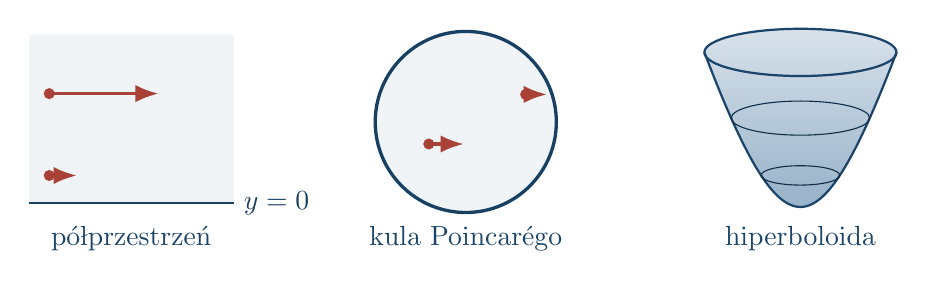
\begin{tikzpicture}[>=Latex,scale=1]
  \begin{scope}[shift={(-4.25,0)}]
    \fill[manifoldblue!7] (-1.3,-1.03) rectangle (1.3,1.10);
    \draw[manifoldblue!70!black,thick] (-1.3,-1.03)--(1.3,-1.03)
      node[right] {$y=0$};
    \fill[manifoldred] (-1.04,-.68) circle (2pt);
    \draw[manifoldred,very thick,->] (-1.04,-.68)--(-.69,-.68);
    \fill[manifoldred] (-1.04,.36) circle (2pt);
    \draw[manifoldred,very thick,->] (-1.04,.36)--(.35,.36);
    \node[manifoldblue!75!black] at (0,-1.48)
       {półprzestrzeń};
  \end{scope}
  \begin{scope}[shift={(0,0)}]
    \fill[manifoldblue!7] (0,0) circle (1.15);
    \draw[manifoldblue!70!black,very thick] (0,0) circle (1.15);
    \fill[manifoldred] (-.47,-.28) circle (2pt);
    \pgfmathsetmacro{\vlen}{1.15*(1-(.47*.47+.28*.28)/(1.15*1.15))/2}
    \draw[manifoldred,very thick,->] (-.47,-.28)--({-.47+\vlen},-.28);
    \fill[manifoldred] (.76,.35) circle (2pt);
    \pgfmathsetmacro{\vlen}{1.15*(1-(.76*.76+.35*.35)/(1.15*1.15))/2}
    \draw[manifoldred,very thick,->] (.76,.35)--({.76+\vlen},.35);
    \node[manifoldblue!75!black] at (0,-1.48)
       {kula Poincarégo};
  \end{scope}
  \begin{scope}[shift={(4.25,-.05)}]
    \pgfmathsetmacro{\htop}{3.4*(sqrt(1+1.22*1.22)-1)-1.03}
    \shade[top color=manifoldblue!18,bottom color=manifoldblue!47]
      plot[domain=-1.22:1.22,samples=61]
        (\x,{3.4*(sqrt(1+\x*\x)-1)-1.03})
      arc[start angle=0,end angle=180,x radius=1.22,y radius=.30]
      --cycle;
    \draw[manifoldblue!75!black,thick]
      plot[domain=-1.22:1.22,samples=61]
        (\x,{3.4*(sqrt(1+\x*\x)-1)-1.03});
    \draw[manifoldblue!75!black,thick] (0,\htop)
      ellipse (1.22 and .30);
    \foreach \rad in {.50,.88}{
      \pgfmathsetmacro{\height}{3.4*(sqrt(1+\rad*\rad)-1)-1.03}
      \draw[manifoldblue!50!black,thin] (0,\height)
        ellipse ({\rad} and {.246*\rad});
    }
    \node[manifoldblue!75!black] at (0,-1.43)
       {hiperboloida};
  \end{scope}
\end{tikzpicture}
\caption{Trzy zapisy tej samej geometrii hiperbolicznej. Czerwone strzałki przedstawiają wektory o długości hiperbolicznej $1$: taki wektor ma różną długość na euklidesowym rysunku półprzestrzeni i kuli. Linia $y=0$ oraz okrąg brzegowy nie należą do rozmaitości. Rysunek hiperboloidy przedstawia fragment górnego płata; jego profil jest gładki także w najniższym punkcie.}
\label{fig:metryki-trzy-modele-hiperboliczne}
\end{figure}

\section{Metryki Schwarzschilda i Kerra: inne znaki}
\label{sec:metryki-lorentzowskie}

\begin{definicja}[Metryka lorentzowska]
\index{metryka lorentzowska@Metryka lorentzowska}
\label{def:metryka-lorentzowska}
Metryka pseudoriemannowska jest gładkim,
symetrycznym, \emph{niezdegenerowanym} tensorem
typu $(0,2)$; dopuszczamy ujemne wartości $g(v,v)$.
W czterech wymiarach metryka o jednym kierunku
ujemnym i trzech dodatnich ma sygnaturę $(-,+,+,+)$
i nazywa się \emph{lorentzowską}.
\end{definicja}

Tu słowo „metryka” oznacza tensor, a nie funkcję
odległości na parach punktów. Dla wektora
czasopodobnego $v$ może być $g(v,v)<0$, a dla
niezerowego wektora światłopodobnego $g(v,v)=0$.
Wzory na riemannowską długość i odległość
z następnej sekcji nie stosują się do całej
takiej czasoprzestrzeni.

W poniższych dwóch przykładach używamy jednostek
geometrycznych $G=c=1$. W jednostkach fizycznych
parametr masy ma wymiar długości:
$M=G M_{\mathrm{fiz}}/c^2$, gdzie
$M_{\mathrm{fiz}}$ jest masą ciała, $G$ stałą
grawitacji, a $c$ prędkością światła. Współrzędna
$t$ ma wtedy wymiar długości ($t=c\,t_{\mathrm{fiz}}$).
Kąty $\theta\in(0,\pi)$ i $\phi\pmod{2\pi}$
oznaczają odpowiednio kąt od osi obrotu oraz azymut.
Symbole $\dd t^2$, $\dd r^2$ itd. oznaczają
kwadraty różniczek współrzędnych w zapisie
symetrycznego tensora $g$.

\begin{przyklad}[Schwarzschild]
\label{prz:metryka-schwarzschild}
W jednostkach geometrycznych $G=c=1$, dla $M>0$
i na obszarze zewnętrznym $r>2M$, metryka ma postać
\begin{equation}\label{eq:schwarzschild}
 g_{\mathrm{Sch}}
 =-\left(1-\frac{2M}{r}\right)\dd t^2
  +\left(1-\frac{2M}{r}\right)^{-1}\dd r^2
  +r^2\bigl(\dd\theta^2+\sin^2\theta\,\dd\phi^2\bigr).
\end{equation}
Parametr $M$ opisuje masę źródła, natomiast $r$
jest \emph{promieniem powierzchniowym}:
sfera określona przez $t,r=\mathrm{const}$
ma pole $4\pi r^2$. Nie jest to ogólnie odległość
zmierzona wzdłuż promienia; z metryki na
$t=\mathrm{const}$ odczytujemy element takiej
odległości $\dd\ell=\dd r/\sqrt{1-2M/r}$.
Współrzędna $t$ jest unormowana tak, aby asymptotycznie, gdy
$r\to\infty$, zgadzać się z czasem własnym obserwatorów
statycznych po przeliczeniu jednostek. Dla obserwatora
o stałych $r,\theta,\phi$ odczytujemy z metryki
$\dd\tau=\sqrt{1-2M/r}\,\dd t$; przy skończonym $r$
czas własny $\tau$ różni się więc od $t$.
Przy $r>2M$ współczynnik $\dd t^2$ jest ujemny,
a trzy przestrzenne są dodatnie, więc sygnatura
wynosi $(-,+,+,+)$. Dla ustalonego $t$
otrzymujemy \emph{riemannowską} metrykę przestrzennego
przekroju
\[
 h_{\mathrm{Sch}}
 =\left(1-\frac{2M}{r}\right)^{-1}\dd r^2
  +r^2\bigl(\dd\theta^2+\sin^2\theta\,\dd\phi^2\bigr).
\]
Na sferze $t,r=\mathrm{const}$ metryka indukowana
to \eqref{eq:metryka-sfery} z $R=r$, więc jej
pole wynosi $4\pi r^2$. Współrzędne sferyczne
nie działają na biegunach, a postać
\eqref{eq:schwarzschild} nie obejmuje $r=2M$;
odpowiednie przedłużenie opisuje się innymi
współrzędnymi.
\end{przyklad}

\begin{przyklad}[Kerr]
\label{prz:metryka-kerr}
Przy $M>0$, $|a|\leq M$ i
$r>r_+:=M+\sqrt{M^2-a^2}$ połóżmy
$\Sigma=r^2+a^2\cos^2\theta$ i
$\Delta=r^2-2Mr+a^2$. W zewnętrznej
dziedzinie współrzędnych Boyera--Lindquista
metrykę zapisuje się zwięźle jako
\begin{align}\label{eq:kerr}
 g_{\mathrm K}
 ={}&-\frac{\Delta}{\Sigma}
       (\dd t-a\sin^2\theta\,\dd\phi)^2
  +\frac{\sin^2\theta}{\Sigma}
       \bigl((r^2+a^2)\dd\phi-a\,\dd t\bigr)^2\\
 &+\frac{\Sigma}{\Delta}\dd r^2
  +\Sigma\,\dd\theta^2.\notag
\end{align}
Tutaj $M$ ponownie jest parametrem masy,
$J$ oznacza moment pędu źródła, a
$a=J/M$ w jednostkach $G=c=1$ jest parametrem
\emph{obrotu} o wymiarze długości
(w zwykłych jednostkach $a=J_{\mathrm{fiz}}/
(M_{\mathrm{fiz}}c)$). Znak $a$ ustala zwrot
obrotu względem rosnącego $\phi$; $a=0$ daje
przypadek bez obrotu. Założenie $|a|\leq M$
zapewnia rzeczywiste pierwiastki $\Delta=0$;
$r_+$ jest większym z nich, czyli współrzędną
zewnętrznego horyzontu. Wielkości $\Sigma$ i
$\Delta$ są skrótami zależnymi od współrzędnych,
nie dodatkowymi parametrami. Współrzędna $r$
nie mierzy tu odległości przestrzennej i przy
$a\ne0$ nie jest także promieniem sfery o polu
$4\pi r^2$; $t,\theta,\phi$ są współrzędnymi
Boyera--Lindquista. Wzór opisuje zewnętrze
horyzontu, a nie całą czasoprzestrzeń.
Kwadrat nawiasu jest kwadratem symetrycznym
$1$-formy. Ponieważ $\Delta>0$ dla $r>r_+$
i $0<\theta<\pi$, cztery wyświetlone
kwadraty mają odpowiednio znaki $-,+,+,+$
(po liniowo niezależnej zamianie pary
$\dd t,\dd\phi$). Istotnie, macierz tej zamiany to
$\left(\begin{smallmatrix}1&-a\sin^2\theta\\-a&r^2+a^2\end{smallmatrix}\right)$,
a jej wyznacznik wynosi $r^2+a^2\cos^2\theta=\Sigma>0$. W szczególności nie jest
to metryka riemannowska.

Sprawdźmy związek ze Schwarzschildem:
dla $a=0$ mamy $\Sigma=r^2$ oraz
$\Delta=r^2(1-2M/r)$; cztery składniki
\eqref{eq:kerr} stają się dokładnie
składnikami \eqref{eq:schwarzschild}.
Dla $a\ne0$ rozwinięcie dwóch pierwszych
kwadratów daje wyraz mieszany
\[
 -\frac{4Mar\sin^2\theta}{\Sigma}
      \,\dd t\,\dd\phi.
\]
W macierzy tensora oznacza to
$g_{t\phi}=-2Mar\sin^2\theta/\Sigma$:
oba wyrazy $g_{t\phi}\dd t\otimes\dd\phi$
i $g_{\phi t}\dd\phi\otimes\dd t$ składają
się na współczynnik podwojony.
Ten wyraz wiąże czas z kierunkiem obrotu.
Przekrój $t=\mathrm{const}$ ma dodatnio określoną
metrykę w podanej dziedzinie. Współczynniki przy
$\dd r^2$ i $\dd\theta^2$ są dodatnie, a współczynnik
przy $\dd\phi^2$ wynosi
\[
 \frac{\sin^2\theta}{\Sigma}
 \bigl((r^2+a^2)^2-a^2\Delta\sin^2\theta\bigr)>0,
\]
ponieważ wyrażenie w nawiasie równa się
$(r^2+a^2)\Sigma+2Mr a^2\sin^2\theta$.
Pomiary przestrzenne zależą jednak od wybranego
przekroju czasoprzestrzeni.
\end{przyklad}

W obu przykładach zapisaliśmy konkretne tensory
i sprawdziliśmy ich znaki oraz prostą zależność
między nimi. Ich wyprowadzenie z równań Einsteina
wymaga aparatu krzywizny, którego jeszcze nie
wprowadziliśmy.

\section{Długość, energia i odległość}
\label{sec:metryka-dlugosc-energia}

\begin{definicja}[Długość i energia krzywej]
\index{dlugosc i energia krzywej@Długość i energia krzywej}
\label{def:dlugosc-energia}
Niech $a<b$, a $\gamma:[a,b]\to(M,g)$ będzie ciągła
i odcinkami klasy $C^1$ (na skończonym podziale przedziału).
Wektor prędkości to $\dot\gamma(t)$, a jego długość,
nazywana także szybkością, wynosi $|\dot\gamma(t)|_g$.
Jej \emph{długość} i
\emph{energia} to odpowiednio
\begin{equation}\label{eq:dlugosc-energia}
 L_g(\gamma)=\int_a^b|\dot\gamma(t)|_g\,\dd t,
 \qquad
 E_g(\gamma)=\frac12\int_a^b
                  |\dot\gamma(t)|_g^2\,\dd t.
\end{equation}
Dla krzywych łączących $p$ z $q$ definiujemy
\begin{equation}\label{eq:odleglosc-riemannowska}
 d_g(p,q)=\inf_{\gamma(a)=p,\ \gamma(b)=q}
                 L_g(\gamma).
\end{equation}
Infimum bierzemy po krzywych odcinkami $C^1$.
Jeśli nie ma takiej krzywej, przyjmujemy $\inf\varnothing=+\infty$.
Zatem dla rozmaitości niespójnej wzór daje metrykę
skończoną osobno na każdej składowej; między różnymi
składowymi ma wartość $+\infty$.
\end{definicja}

Metryka $g$ mierzy wektor prędkości w każdym
punkcie, długość sumuje te pomiary wzdłuż
\emph{jednej} drogi, a $d_g$ szuka najkrótszej
możliwej długości. Infimum nie zakłada jeszcze,
że istnieje krzywa, która je osiąga.

\begin{stwierdzenie}[Zmiana parametru i energia]
\label{prop:energia-dlugosc}
Jeśli $h:[c,d]\to[a,b]$ jest rosnącym dyfeomorfizmem
klasy $C^1$, to
$L_g(\gamma\circ h)=L_g(\gamma)$.
Ponadto
\begin{equation}\label{eq:energia-cauchy}
 L_g(\gamma)^2\leq 2(b-a)E_g(\gamma),
\end{equation}
z równością wtedy i tylko wtedy, gdy prędkość
$|\dot\gamma|_g$ jest stała prawie wszędzie.
Dla regularnej krzywej klasy $C^1$, czyli takiej, że
$\dot\gamma(t)\ne0$, istnieje przeparametryzowanie klasy
$C^1$ ze stałą szybkością. Osiąga ono najmniejszą energię
wśród wszystkich regularnych przeparametryzowań na
ustalonym $[a,b]$. Dla krzywej odcinkami regularnej
odpowiednie przeparametryzowanie jest odcinkami klasy $C^1$.
\end{stwierdzenie}
\begin{proof}
Reguła łańcuchowa daje
$(\gamma\circ h)'(s)=\dot\gamma(h(s))h'(s)$.
Ponieważ $h'>0$, jednorodność normy i podstawienie
$t=h(s)$ dają
\[
 L_g(\gamma\circ h)
 =\int_c^d|\dot\gamma(h(s))|_g h'(s)\,\dd s
 =\int_a^b|\dot\gamma(t)|_g\,\dd t.
\]
Dla malejącego dyfeomorfizmu ten sam rachunek używa
$|h'|=-h'$ i odwróconych granic całkowania, więc długość
także się nie zmienia. Dla energii w pierwszej całce występuje
$(h')^2$, a więc podstawienie nie usuwa całego
czynnika: energia na ogół się zmienia.
Nierówność Cauchy'ego--Schwarza dla funkcji
$1$ i $|\dot\gamma|_g$ na $[a,b]$ daje
\[
 \left(\int_a^b|\dot\gamma|_g\,\dd t\right)^2
 \leq\left(\int_a^b1\,\dd t\right)
      \left(\int_a^b|\dot\gamma|_g^2\,\dd t\right).
\]
To \eqref{eq:energia-cauchy}. Warunek równości
w Cauchym--Schwarzu oznacza, że obie funkcje
są proporcjonalne prawie wszędzie, czyli
$|\dot\gamma|_g$ jest stała prawie wszędzie.
Dla regularnej krzywej $|\dot\gamma|_g>0$;
funkcja
$s(t)=a+\frac{b-a}{L_g(\gamma)}
               \int_a^t|\dot\gamma(\tau)|_g\,\dd\tau$
jest rosnąca, przenosi końce przedziału na
siebie, a reguła łańcuchowa pokazuje,
że $\gamma\circ s^{-1}$ ma stałą prędkość
$L_g(\gamma)/(b-a)$. Osiąga zatem dolną granicę
energii $L_g(\gamma)^2/[2(b-a)]$.
\end{proof}

\begin{twierdzenie}[Odległość riemannowska jest metryką]
\label{thm:odleglosc-jest-metryka}
Jeżeli $M$ jest spójna, to \eqref{eq:odleglosc-riemannowska}
przyjmuje skończone wartości, spełnia aksjomaty
metryki przestrzeni metrycznej $(M,d_g)$
i wyznacza pierwotną topologię rozmaitości.
\end{twierdzenie}
\begin{proof}
W wymiarze $0$ spójna rozmaitość składa się z jednego
punktu i teza jest natychmiastowa. Załóżmy $n\geq1$.
Relacja „można połączyć krzywą odcinkami $C^1$” jest
relacją równoważności. Każda jej klasa jest otwarta:
w małej kuli współrzędnych, a przy brzegu w półkuli,
można połączyć dwa punkty odcinkiem prostym w mapie.
Dopełnienie klasy także jest otwarte, jako suma innych
klas. Ze spójności wynika, że jest tylko jedna klasa.
Na każdym ze skończenie wielu kawałków takiej krzywej
prędkość i współczynniki metryki są ciągłe na zwartym
przedziale, więc długość jest skończona.
Zatem $d_g(p,q)<\infty$.

Długości są nieujemne, stała krzywa ma
długość zero, odwrócenie kierunku zachowuje
długość, a długości sklejonych krzywych
dodają się. Biorąc infima (i drogi o długości
dowolnie bliskiej obu infimom), otrzymujemy
$d_g(p,p)=0$, symetrię i nierówność trójkąta.

Zostało najważniejsze: $d_g(p,q)>0$ dla $p\ne q$.
Wybierzmy mapę $x$ z $x(p)=0$ i domkniętą
kulę współrzędnych $\overline B_{2r}$ leżącą
w obrazie tej mapy. Jeśli $p\in\partial M$, wybieramy
mapę przybrzegową z $x(p)=0$ i w całym poniższym
rachunku zastępujemy $B_\rho$ przez
$B_\rho\cap\{x^n\geq0\}$. Te półkule są wypukłe,
więc odcinki używane w dowodzie pozostają w $M$.
„Wyjście z kuli” oznacza wtedy przekroczenie jej
sferycznej części brzegu wewnątrz półprzestrzeni.
Na zwartym zbiorze
$x^{-1}(\overline B_{2r})$ dodatnia określoność
i ciągłość macierzy $G$ dają stałe $c,C>0$,
takie że
\[
 c|w|\leq\sqrt{w^{\mathsf T}G(x)w}\leq C|w|
 \quad (x\in\overline B_{2r}).
\]
Istnienie wspólnego $c$ można zobaczyć,
minimalizując $w^{\mathsf T}G(x)w$ po zwartym
iloczynie $\overline B_{2r}\times S^{n-1}$.

Jeśli $q$ leży w $x^{-1}(B_r)$, droga z $p$
do $q$ pozostająca w $B_{2r}$ ma długość
co najmniej $c|x(q)|$, bo długość euklidesowa
drogi jest nie mniejsza niż przemieszczenie
końców. Droga wychodząca z $B_{2r}$ ma do
pierwszego wyjścia długość co najmniej $2cr$,
więc również co najmniej $c|x(q)|$.
Jeśli $q$ leży poza $x^{-1}(B_r)$, każda droga
do $q$ musi najpierw opuścić $B_r$, zatem
ma długość co najmniej $cr$. Oba przypadki
dają dodatnią odległość od $p$.

Te same oszacowania porównują topologie.
Dla $q$ w $B_r$ odcinek prosty od $0$ do $x(q)$
daje $d_g(p,q)\leq C|x(q)|$.
Z drugiej strony kula metryczna
$B_{d_g}(p,cr)$ leży w $x^{-1}(B_r)$,
a na niej $d_g(p,q)\geq c|x(q)|$.
Zbieżność w mapie i zbieżność dla $d_g$
są więc lokalnie równoważne.
\end{proof}

\begin{przyklad}[Niezupełność i brzeg modelu hiperbolicznego]
Przedział $(0,1)$ z $g=\dd x^2$ ma zwykłą
odległość $|p-q|$, ale ciąg $1/j$, $j\geq2$, jest
Cauchy'ego i nie zbiega w tym przedziale.
Samo istnienie $g$ nie zapewnia zupełności.

W półprzestrzeni hiperbolicznej pionowa droga
od $(x,y_0)$ do $(x,y_1)$ ma długość
$|\log(y_1/y_0)|$. Każda inna droga ma
\[
 L_g(\gamma)\geq\int\frac{|y'(t)|}{y(t)}\,\dd t
 \geq\left|\int\frac{y'(t)}{y(t)}\,\dd t\right|
 =|\log(y_1/y_0)|,
\]
więc jest to rzeczywista odległość tych punktów.
Granica $y=0$ leży nieskończenie daleko.
Podobnie w kuli Poincarégo
$d_g(0,u)=\log\frac{1+|u|}{1-|u|}$,
bo na każdej drodze $\gamma$ funkcja
$\rho(t)=|\gamma(t)|$ jest absolutnie ciągła
i $|\rho'|\leq|\dot\gamma|$ prawie wszędzie.
Stąd
\[
 L_g(\gamma)\geq\int\frac{2|\rho'|}{1-\rho^2}\,\dd t
 \geq\left|\int\frac{2\rho'}{1-\rho^2}\,\dd t\right|
 =\int_0^{|u|}\frac{2\,\dd s}{1-s^2}
 =\log\frac{1+|u|}{1-|u|}.
\]
Promień od $0$ do $u$ osiąga tę dolną granicę.
\end{przyklad}

\section{Objętość wyznaczona przez metrykę}
\label{sec:metryka-objetosc}

Jeden wektor ma długość; $n$ niezależnych
wektorów stycznych rozpinających maleńki
równoległościan ma objętość. W bazie
ortogonalnej jest to iloczyn długości.
W dowolnej bazie odpowiednią liczbę
zawiera wyznacznik macierzy Grama.

\begin{definicja}[Element objętości i miara riemannowska]
\index{element objetosci i miara riemannowska@Element objętości i miara riemannowska}
\label{def:miara-riemannowska}
W mapie $x$ na $(M^n,g)$ \emph{element objętości}
jest dodatnią gęstością
\begin{equation}\label{eq:element-objetosci}
 \dd\mu_g=\sqrt{\det(g_{ij}(x))}\,
                 |\,\dd x^1\cdots\dd x^n\,|.
\end{equation}
Przez całkowanie tej gęstości w mapach
otrzymujemy miarę borelowską $\mu_g$.
Dla funkcji borelowskiej $f\geq0$ lub funkcji całkowalnej,
o nośniku zawartym w jednej mapie,
\[
 \int_M f\,\dd\mu_g
  =\int_{x(U)} f(x^{-1}(u))
      \sqrt{\det G(u)}\,\dd u^1\cdots\dd u^n.
\]
Ogólną całkę definiujemy z podziałem jedności:
dla funkcji nieujemnej dopuszczamy wartość $+\infty$,
a dla funkcji ze znakiem wymagamy $\int_M|f|\,\dd\mu_g<\infty$.
Sam zwarty nośnik funkcji mierzalnej nie zapewnia całkowalności.
W wymiarze $0$ przyjmujemy wyznacznik macierzy pustej równy $1$;
$\mu_g$ jest wtedy miarą liczącą punkty. Na rozmaitości zorientowanej
\emph{forma objętościowa} ma w dodatniej mapie postać
$\mathrm{vol}_g=\sqrt{\det G}\,
 \dd x^1\wedge\cdots\wedge\dd x^n$.
Dla $n=0$ forma objętościowa ma w punkcie wartość
$\varepsilon_p\in\{1,-1\}$ zadaną jego orientacją;
całkowanie z tą samą orientacją daje dodatnią masę $1$.
\end{definicja}

Kreski pionowe w \eqref{eq:element-objetosci}
oznaczają gęstość: zmiana orientacji nie zmienia
miary. Forma $\mathrm{vol}_g$ ma natomiast znak
zależny od orientacji. Dlatego pole powierzchni
możemy obliczyć również na rozmaitości
nieorientowalnej, choć nie ma na niej globalnej
formy objętościowej.

\begin{twierdzenie}[Niezależność elementu objętości od mapy]
\label{thm:element-objetosci-globalny}
Wzór \eqref{eq:element-objetosci} daje
jednoznaczną miarę na $M$, niezależną od atlasu
i podziału jedności. Jeżeli $F:(M,g)\to(N,h)$
jest izometrią, czyli dyfeomorfizmem z $F^*h=g$,
to $\mu_g(F^{-1}A)=\mu_h(A)$ dla zbiorów
borelowskich $A\subset N$.
\end{twierdzenie}
\begin{proof}
Na przecięciu map niech $x=x(y)$ i
$J=\partial x/\partial y$. Ze
Stwierdzenia~\ref{prop:metryka-zmiana} wynika
\[
 \sqrt{\det G_y}
   =|\det J|\sqrt{\det G_x}.
\]
To dokładnie czynnik w twierdzeniu o zmianie
zmiennych w całce Lebesgue'a, więc obliczenia
tego samego zbioru w obu mapach są zgodne.
Wybierzmy przeliczalne pokrycie mapami
$(U_j)$, a mierzalny zbiór $A$ rozbijmy
na rozłączne fragmenty
$A\cap U_1$,
$A\cap(U_2\setminus U_1)$ itd.
Sumujemy ich lokalne miary. Na przecięciach
otrzymalibyśmy te same liczby w innych mapach,
więc wynik nie zależy od tego rozbicia;
lokalna addytywność całki daje przeliczalną
addytywność globalną. Analogicznie porównujemy
dwa podziały jedności przez ich wspólne
rozdrobnienie.

Dla izometrii macierz jej różniczki spełnia
w lokalnych bazach $G_M=(DF)^{\mathsf T}G_N(DF)$.
Poprzedni rachunek wyznaczników i podstawienie
w całce pokazują
$\int_M(f\circ F)\dd\mu_g=\int_N f\dd\mu_h$
dla nieujemnych funkcji mierzalnych $f$.
Wstawiając funkcję charakterystyczną $A$,
otrzymujemy tezę o miarach.
\end{proof}

\begin{przyklad}[Gęstości w modelach]
Ze \eqref{eq:metryka-sfery} otrzymujemy
$\dd\mu_{S_R^2}=R^2\sin\theta\,
\dd\theta\,\dd\phi$ dla $0<\theta<\pi$,
a stąd
$\operatorname{Pole}(S_R^2)
=\int_0^{2\pi}\int_0^\pi
R^2\sin\theta\,\dd\theta\,\dd\phi=4\pi R^2$.
Parametry $0<\theta<\pi$, $0<\phi<2\pi$ pomijają
bieguny i jeden południk. Zbiory te mają zerową miarę
powierzchniową: w regularnych mapach są punktami lub
wykresami jednowymiarowymi, zerowymi dla dwuwymiarowej
miary Lebesgue'a z twierdzenia Fubiniego. Gładka gęstość
nie zmienia tej zerowości. Nie całkujemy więc przez
osobliwość mapy; dodajemy jedynie zbiór miary zero.
W półprzestrzeni hiperbolicznej macierz
metryki jest $y^{-2}I_n$, więc
$\dd\mu_{\mathbb H}=y^{-n}\dd x^1\cdots
\dd x^{n-1}\dd y$.
W kuli Poincarégo gęstość wynosi
$(2/(1-|u|^2))^n\dd u^1\cdots\dd u^n$.
W przestrzennych współrzędnych $z$ hiperboloidy
z~\eqref{eq:hiperboloida-wspolrzedne-metryka}
wyznacznik obliczony w
\eqref{eq:hiperboloida-macierz-odwrotna} daje
\[
 \dd\mu_{\mathcal H}
  =\frac{\dd z^1\cdots\dd z^n}{\sqrt{1+|z|^2}}.
\]
Podana formuła dotyczy \emph{metryki indukowanej
na hiperboloidzie}, nie miary otaczającej
przestrzeni Minkowskiego. Izometrie $P$ i $F$
z Przykładu~\ref{prz:trzy-modele-hiperboliczne}
przekształcają te trzy gęstości w siebie.

Dla przestrzennego przekroju Schwarzschilda
z Przykładu~\ref{prz:metryka-schwarzschild}
macierz $h_{\mathrm{Sch}}$ jest diagonalna:
\[
 \det h_{\mathrm{Sch}}
  =\frac{r^4\sin^2\theta}{1-2M/r},
 \qquad
 \dd\mu_{h_{\mathrm{Sch}}}
  =\frac{r^2\sin\theta}{\sqrt{1-2M/r}}\,
       \dd r\,\dd\theta\,\dd\phi.
\]
Jest to \emph{trójwymiarowa} miara wybranego
przekroju, a nie miara całej metryki lorentzowskiej.
\end{przyklad}

\section{Metryka indukowana i całki po podrozmaitości}
\label{sec:metryka-indukowana}

\begin{definicja}[Metryka indukowana]
\index{metryka indukowana@Metryka indukowana}
\label{def:metryka-indukowana}
Niech $i:S^k\hookrightarrow(M^n,g)$ będzie
gładką podrozmaitością, $k\leq n$.
Na $S$ definiujemy $h=i^*g$:
\[
 h_p(v,w)=g_{i(p)}(\dd i_pv,\dd i_pw)
 \quad(v,w\in T_pS).
\]
Ponieważ $\dd i_p$ jest iniektywna, $h$ jest
metryką riemannowską. Miara $\mu_h$ na $S$
pozwala całkować funkcję $f:S\to\R$;
oznaczenie $\int_S f\,\dd A_g$ stosujemy,
gdy $k=n-1$.
\end{definicja}

Parametryzacja $F:U\subset\R^k\to S$
wybiera wektory $F_1,\ldots,F_k$ styczne
do powierzchni. Macierz Grama tych wektorów
wyznacza rzeczywisty rozmiar
obrazu małego prostokąta współrzędnych.

\begin{figure}[!htbp]
\centering
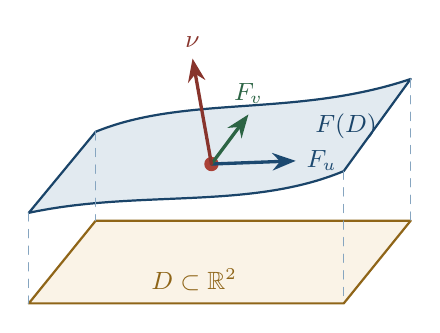
\begin{tikzpicture}[>=Stealth,line cap=round,line join=round]
 \fill[manifoldgold!11]
   (0,0)--(4.0,0)--(4.85,1.05)--(.85,1.05)--cycle;
 \draw[manifoldgold!70!black,thick]
   (0,0)--(4.0,0)--(4.85,1.05)--(.85,1.05)--cycle;
 \fill[manifoldblue!13]
   (0,1.15) .. controls (1.4,1.45) and (2.8,1.18) .. (4,1.68)
   --(4.85,2.85)
   .. controls (3.4,2.36) and (2.0,2.65) .. (.85,2.18)--cycle;
 \draw[manifoldblue!75!black,thick]
   (0,1.15) .. controls (1.4,1.45) and (2.8,1.18) .. (4,1.68)
   --(4.85,2.85)
   .. controls (3.4,2.36) and (2.0,2.65) .. (.85,2.18)--cycle;
 \draw[manifoldblue!55,dashed]
   (.85,2.18)--(.85,1.05)
   (4,1.68)--(4,0)
   (4.85,2.85)--(4.85,1.05)
   (0,1.15)--(0,0);
 \coordinate (p) at (2.32,1.77);
 \fill[manifoldred] (p) circle (2.6pt);
 \draw[->,line width=1.2pt,manifoldblue!80!black]
   (p)--(3.39,1.81) node[right,font=\small] {$F_u$};
 \draw[->,line width=1.2pt,manifoldgreen!80!black]
   (p)--(2.79,2.40) node[above,font=\small] {$F_v$};
 \draw[->,line width=1.2pt,manifoldred!80!black]
   (p)--(2.08,3.11) node[above,font=\small] {$\nu$};
 \node[manifoldgold!70!black,font=\small] at (2.10,.30) {$D\subset\R^2$};
 \node[manifoldblue!75!black,font=\small] at (4.03,2.25) {$F(D)$};
\end{tikzpicture}
\caption{Parametryzacja unosi obszar parametrów $D$
na powierzchnię. Wektory $F_u,F_v$ wyznaczają
element pola $\sqrt{\det(g(F_a,F_b))}\,\dd u\,\dd v$;
normalna $\nu$ pozwala dodatkowo mierzyć strumień.}
\label{fig:metryka-indukowana-pole}
\end{figure}

\begin{uwaga}[Interpretacja ortogonalna wiązki normalnej]
Niech $S\subset M$ będzie podrozmaitością zanurzoną i niech
$g$ będzie metryką riemannowską na $M$. Dla każdego $p\in S$
definiujemy \emph{przestrzeń normalną} jako dopełnienie
ortogonalne przestrzeni stycznej:
\[
\nu_p^\perp S:=(T_pS)^\perp
=\{v\in T_pM:\ g_p(v,w)=0
\text{ dla każdego }w\in T_pS\}.
\]
Dodatnia określoność metryki daje rozkład ortogonalny
\[
T_pM=T_pS\oplus\nu_p^\perp S.
\]
Przestrzenie te tworzą \emph{ortogonalną wiązkę normalną}
\[
\nu^\perp S:=\bigsqcup_{p\in S}\nu_p^\perp S
\subset TM|_S,
\]
a na poziomie wiązek otrzymujemy
\[
TM|_S=TS\oplus\nu^\perp S.
\]

Uzasadnijmy, że $\nu^\perp S$ jest gładką podwiązką.
Niech $(X_1,\ldots,X_k)$ będzie lokalną bazą gładkich
sekcji $TS$. Macierz Grama
\[
G(p)=\bigl(g_p(X_a(p),X_b(p))\bigr)_{a,b=1}^k
\]
jest gładka i odwracalna. Rzut ortogonalny na $T_pS$
ma zatem postać
\[
P_p(v)=
\sum_{a,b=1}^k
g_p(v,X_a(p))(G(p)^{-1})^{ab}X_b(p).
\]
Zależy on gładko od $p$, więc również
$\operatorname{id}-P$ jest gładkim rzutowaniem
wiązek o stałym rzędzie $n-k$, gdzie $n=\dim M$.
Jego obrazem jest $\nu^\perp S$, co dowodzi,
że jest ona gładką podwiązką $TM|_S$.

Rozkład ortogonalny pozwala ponadto utożsamić
kanoniczną wiązkę normalną ilorazową
$\nu S=TM|_S/TS$ z $\nu^\perp S$.
Istotnie, odwzorowanie
\[
\nu^\perp S\longrightarrow\nu S,
\qquad
v\longmapsto[v],
\]
jest izomorfizmem wiązek wektorowych: na każdym
włóknie jest liniowe i różnowartościowe, ponieważ
$T_pS\cap\nu_p^\perp S=\{0\}$, oraz surjektywne
na mocy rozkładu ortogonalnego.

W przeciwieństwie do konstrukcji ilorazowej,
wybór podwiązki $\nu^\perp S\subset TM|_S$
zależy od metryki $g$. W ten sposób metryka
pozwala reprezentować klasy wektorów normalnych
przez jednoznacznie wyznaczone wektory prostopadłe
do $T_pS$.
\end{uwaga}


\begin{twierdzenie}[Wzór parametryczny na całkę]
\label{thm:calka-podrozmaitosc}
Jeżeli $F$ jest parametryzacją kawałka
podrozmaitości, jeden raz pokrywającą
rozważany fragment, i $f$ jest całkowalna
o nośniku w tym fragmencie, to
\begin{equation}\label{eq:calka-podrozmaitosc}
 \int_{F(U)}f\,\dd\mu_h
 =\int_U f(F(u))
   \sqrt{\det\bigl(g(F_a,F_b)\bigr)_{a,b=1}^k}
                      \,\dd u^1\cdots\dd u^k .
\end{equation}
Dla $M=\R^3$ z metryką euklidesową i $k=2$ czynnik pod pierwiastkiem
jest $|F_u\times F_v|^2$.
\end{twierdzenie}
\begin{proof}
Z definicji cofnięcia tensora
$h_{ab}(u)=g_{F(u)}(\partial_aF,\partial_bF)$.
Podstawmy tę macierz do
\eqref{eq:element-objetosci} w wymiarze $k$:
dostajemy dokładnie prawą stronę
\eqref{eq:calka-podrozmaitosc}.
Dlaczego jest to pole, a nie sztuczny czynnik?
Wybierzmy ortonormalną bazę w $T_{F(u)}M$
i zapiszmy kolumny $F_a$ w macierzy $J$.
Wówczas $(h_{ab})=J^{\mathsf T}J$.
Ortogonalizując kolumny metodą Grama--Schmidta,
otrzymujemy prostopadłe wektory o długościach
$\ell_1,\ldots,\ell_k$. Ortogonalna zmiana
kierunków i dodawanie wcześniejszych kolumn
do późniejszych nie zmieniają objętości
rozpiętego równoległościanu. Zatem jego
$k$-wymiarowa objętość wynosi
$\ell_1\cdots\ell_k$ i jednocześnie
$\det(J^{\mathsf T}J)=\ell_1^2\cdots\ell_k^2$.
Zmiana parametrów $u=u(v)$ mnoży ten czynnik
przez $|\det(\partial u/\partial v)|$,
jak w Stwierdzeniu~\ref{prop:metryka-zmiana};
twierdzenie o podstawieniu pokazuje
niezależność wyniku od parametryzacji.
W $\R^3$ tożsamość
$|F_u\times F_v|^2
=|F_u|^2|F_v|^2-(F_u\cdot F_v)^2$
jest wyznacznikiem macierzy Grama $2\times2$.
\end{proof}

Jeśli parametryzacja pokrywa fragment kilka
razy, prawa strona liczy go z krotnością.
Dla całej podrozmaitości używamy map
i podziału jedności, żeby każdy punkt
został policzony tylko raz. Dla $k=1$
wzór jest całką po łuku
$\int f(\gamma(t))|\dot\gamma(t)|_g\,\dd t$;
dla $k=n$ jest zwykłą całką objętościową.

\begin{przyklad}[Wykres funkcji i paraboloida]
\label{prz:calka-po-wykresie}
Dla $F(x,y)=(x,y,f(x,y))$ w euklidesowej $\R^3$
wektory styczne to $(1,0,f_x)$ i $(0,1,f_y)$,
a ich macierz Grama to
\[
 \begin{pmatrix}1+f_x^2&f_xf_y\\
                 f_xf_y&1+f_y^2\end{pmatrix}.
\]
Jej wyznacznik jest $1+f_x^2+f_y^2$, więc
\begin{equation}\label{eq:calka-wykres}
 \int_{\operatorname{graf}(f|_D)}\psi\,\dd A
 =\int_D\psi(x,y,f(x,y))
        \sqrt{1+f_x^2+f_y^2}\,\dd x\,\dd y.
\end{equation}
Pierwiastek wyraża nachylenie: skośny fragment
ma większe pole niż jego rzut na płaszczyznę.

Weźmy $f=x^2+y^2$ nad dyskiem $x^2+y^2\leq a^2$.
Współrzędne biegunowe dają pole wykresu
\[
 \int_0^{2\pi}\!\int_0^a
   \sqrt{1+4r^2}\,r\,\dd r\,\dd\phi
 =\frac{\pi}{6}\bigl((1+4a^2)^{3/2}-1\bigr).
\]
W ostatnim kroku użyliśmy podstawienia
$s=1+4r^2$, $\dd s=8r\,\dd r$.
\end{przyklad}

\begin{przyklad}[Całka skalarna po sferze]
Na $S_R^2$ obliczmy całkę z funkcji $z^2$.
Ponieważ $z=R\cos\theta$, mamy
\[
 \int_{S_R^2}z^2\,\dd A
 =R^4\int_0^{2\pi}\!\int_0^\pi
       \cos^2\theta\sin\theta\,\dd\theta\,\dd\phi
 =\frac{4\pi R^4}{3}.
\]
Wewnętrzna całka wynosi $2/3$ po podstawieniu
$s=\cos\theta$. Jest to całka \emph{skalarna};
nie potrzebujemy wybrać orientacji sfery.
\end{przyklad}

\subsection*{Całki skierowane: dlaczego pojawia się znak?}
\label{subsec:calki-skierowane}

Pole powierzchni i strumień odpowiadają na dwa różne
pytania. W całce skalarnej
$\int_S f\,\dd A$ liczymy wielkość fragmentów
powierzchni: wzór~\eqref{eq:calka-podrozmaitosc}
zawiera dodatni pierwiastek z wyznacznika Grama.
Odwrócenie parametrów nie zmienia wyniku.
W \emph{całce skierowanej} pytamy, ile pola
wektorowego przechodzi przez powierzchnię
w \emph{wybranym kierunku}. Musimy ustalić,
która strona jest dodatnia; odwrócenie
normalnej zmienia znak strumienia.

\begin{przyklad}[Całka skierowana po krzywej]
\label{prz:calka-skierowana-krzywa}
Niech $\gamma:[a,b]\to\R^3$ ma wybrany kierunek
przebiegu, a $X=(P,Q,R)$ będzie polem wektorowym.
Całka skierowana wzdłuż
krzywej (często zwana \emph{całką krzywoliniową
drugiego rodzaju}) ma wzór
\begin{equation}\label{eq:calka-skierowana-krzywa}
 \int_\gamma X\cdot\dd\mathbf r
 =\int_a^b X(\gamma(t))\cdot\dot\gamma(t)\,\dd t
 =\int_\gamma(P\,\dd x+Q\,\dd y+R\,\dd z).
\end{equation}
Jeżeli $\bar\gamma(t)=\gamma(a+b-t)$, to
$\dot{\bar\gamma}(t)=-\dot\gamma(a+b-t)$.
Podstawienie $s=a+b-t$ w całce daje
$\int_{\bar\gamma}X\cdot\dd\mathbf r
=-\int_\gamma X\cdot\dd\mathbf r$.
Natomiast $\int_\gamma f\,\dd s
=\int_a^b f(\gamma(t))|\dot\gamma(t)|\,\dd t$
nie zmienia się przy odwróceniu przebiegu:
norma usuwa znak prędkości.
\end{przyklad}

\begin{przyklad}[Całka skierowana po powierzchni]
\label{prz:calka-skierowana-powierzchnia}
Niech $\Phi:D\subset\R^2\to S\subset\R^3$
będzie regularną parametryzacją pokrywającą rozważany
fragment jednokrotnie, a orientację
$S$ wybierzmy przez normalną
$\nu=(\Phi_u\times\Phi_v)/|\Phi_u\times\Phi_v|$.
Dla pola $X$ \emph{strumień} przez $S$ wynosi
\begin{equation}\label{eq:calka-skierowana-powierzchnia}
 \int_S X\cdot\dd\mathbf S
 :=\int_S X\cdot\nu\,\dd A
 =\int_D X(\Phi(u,v))\cdot
           (\Phi_u\times\Phi_v)\,\dd u\,\dd v.
\end{equation}
To ten sam element pola co na
Rysunku~\ref{fig:metryka-indukowana-pole},
ale z kierunkiem normalnej.
Zamiana $u$ z $v$ zmienia
$\Phi_u\times\Phi_v$ na jego przeciwieństwo;
czynnik $|\Phi_u\times\Phi_v|$ w całce skalarnej
nie zmieniłby się.

Dla wykresu $\Phi(u,v)=(u,v,f(u,v))$
i stałego pola pionowego $X=(0,0,1)$ mamy
$\Phi_u\times\Phi_v=(-f_u,-f_v,1)$.
Przy normalnej ku górze
$\int_S X\cdot\dd\mathbf S=\int_D1\,\dd u\,\dd v
=\operatorname{Pole}(D)$; przy normalnej ku dołowi
wynik ma znak minus. Natomiast
$\int_S1\,\dd A
=\int_D\sqrt{1+f_u^2+f_v^2}\,\dd u\,\dd v$
jest dodatnie przy obu orientacjach.
\end{przyklad}

\begin{stwierdzenie}[Związek z całką z formy]
\label{prop:calka-skierowana-forma}
W zorientowanej $\R^3$ ze standardową
formą objętości $\mathrm{vol}=\dd x\wedge\dd y
\wedge\dd z$ polu $X=(P,Q,R)$ odpowiada $2$-forma
\[
 \beta=\iota_X\mathrm{vol}
 =P\,\dd y\wedge\dd z+
  Q\,\dd z\wedge\dd x+
  R\,\dd x\wedge\dd y.
\]
Wówczas $\int_{(S,o)}\beta
=\int_S X\cdot\nu_o\,\dd A$.
Na zorientowanej $(M^n,g)$
$\dd\mu_g=|\mathrm{vol}_{g,o}|$ w sensie gęstości,
a więc
\[
 \int_M f\,\dd\mu_g
 =\int_{(M,o)}f\,\mathrm{vol}_{g,o}.
\]
Jeśli \emph{ta sama} forma najwyższego stopnia
$\omega$ jest całkowana po $M$ z orientacją
przeciwną $-o$, to
$\int_{(M,-o)}\omega=-\int_{(M,o)}\omega$.
\end{stwierdzenie}
\begin{proof}
Z definicji cofnięcia form z
Rozdziału~\ref{ch:formy-de-rham},
\[
 (\Phi^*\beta)(\partial_u,\partial_v)
 =\mathrm{vol}\bigl(X(\Phi),\Phi_u,\Phi_v\bigr)
 =X(\Phi)\cdot(\Phi_u\times\Phi_v).
\]
Całkowanie po $D$ daje
\eqref{eq:calka-skierowana-powierzchnia}.
Dla krzywej analogicznie
$\gamma^*(P\,\dd x+Q\,\dd y+R\,\dd z)
=X(\gamma)\cdot\dot\gamma\,\dd t$.

W dodatniej mapie
$\mathrm{vol}_{g,o}=\sqrt{\det G}\,
\dd x^1\wedge\cdots\wedge\dd x^n$,
podczas gdy wzór~\eqref{eq:element-objetosci}
na $\dd\mu_g$ zawiera wartość bezwzględną
wyznacznika zmiany współrzędnych. Stąd
równość całek dla \emph{zgodnie} wybranych
orientacji i formy. Przy odwróceniu samej
orientacji dodatnie mapy stają się ujemne,
więc całka z ustalonej formy zmienia znak.
Gdybyśmy jednocześnie zastąpili
$\mathrm{vol}_{g,o}$ nową dodatnią formą
$\mathrm{vol}_{g,-o}=-\mathrm{vol}_{g,o}$,
oba znaki by się zniosły; całka z gęstości
pozostałaby ta sama. Właśnie dlatego
przy strumieniu trzeba podać \emph{stronę}
powierzchni, a przy samym polu powierzchni nie.
\end{proof}

\section{Miara Hausdorffa: pomiar bez map i pochodnych}
\label{sec:miara-hausdorffa}

Miara riemannowska wykorzystuje gładkie mapy
i wyznacznik macierzy metryki. Miara Hausdorffa
wychodzi tylko od \emph{odległości}: pokrywamy zbiór
coraz mniejszymi częściami i sumujemy odpowiednie
potęgi ich średnic. Dzięki temu ma sens również
na zbiorach, które nie są rozmaitościami.

\begin{definicja}[Miara Hausdorffa]
\index{miara hausdorffa@Miara Hausdorffa}
\label{def:miara-hausdorffa}
Niech $(X,d)$ będzie przestrzenią metryczną,
$s\geq0$, a $A\subset X$.
Przez $\operatorname{diam}_d U$ oznaczmy
$\sup\{d(x,y):x,y\in U\}$. Kładziemy
\begin{align}\label{eq:hausdorff-def}
 \mathcal H^s_{d,\delta}(A)
 &=c_s\inf\left\{
       \sum_{j=1}^{\infty}(\operatorname{diam}_d U_j)^s:
       A\subset\bigcup_j U_j,\
       \operatorname{diam}_d U_j<\delta\right\},\\
 \mathcal H^s_d(A)
 &=\lim_{\delta\downarrow0}
                  \mathcal H^s_{d,\delta}(A).
 \notag
\end{align}
Pokrycia mogą być skończone lub przeliczalne;
puste składniki pomijamy, a puste pokrycie zbioru
pustego ma koszt $0$. Przy braku dopuszczalnego
pokrycia infimum wynosi $+\infty$.
Dla $s=k$ całkowitego stosujemy normalizację
$c_k=\omega_k/2^k$, gdzie $\omega_k$
jest objętością euklidesowej kuli jednostkowej
w $\R^k$ ($\omega_0=1$). Dla innych $s$
można wziąć dowolne dodatnie $c_s$;
wartość \emph{wymiaru Hausdorffa}
$\dim_{\mathrm H}A
=\inf\{s:\mathcal H^s_d(A)=0\}$
nie zależy od tego wyboru.
\end{definicja}

Gdy $\delta$ maleje, pokryć dopuszczalnych
jest mniej, więc infimum nie maleje:
granica w \eqref{eq:hausdorff-def} istnieje,
choć może być nieskończona.
Dla $s=0$ przyjmujemy $0^0=1$ dla
niepustego zbioru w pokryciu;
$\mathcal H^0$ liczy punkty: zbiór $N$ różnych punktów
wymaga co najmniej $N$ składników dla $\delta$ mniejszego
niż ich minimalna wzajemna odległość, a pokrycie
singletonami ma koszt $N$. Dla zbioru nieskończonego
stosujemy dolne oszacowanie do dowolnie dużych
skończonych podzbiorów i dostajemy $+\infty$.
Na prostym odcinku z odległością euklidesową $\mathcal H^1$ jest
jego długością, a na gładkiej powierzchni euklidesowej
$\mathcal H^2$ jest polem.

\begin{stwierdzenie}[Dlaczego otrzymujemy miarę borelowską]
\label{prop:hausdorff-borel}
Funkcja $\mathcal H^s_d$ jest miarą zewnętrzną.
Jeśli $d(A,B):=\inf\{d(a,b):a\in A,b\in B\}>0$, to
\[
 \mathcal H^s_d(A\cup B)=\mathcal H^s_d(A)+\mathcal H^s_d(B).
\]
Wszystkie zbiory borelowskie są dla niej mierzalne,
a na nich $\mathcal H^s_d$ jest przeliczalnie addytywna.
\end{stwierdzenie}
\begin{proof}
Dla ustalonego $\delta$ monotoniczność i wartość zero
na zbiorze pustym wynikają z definicji. Pokrywając
każdy $A_i$ z kosztem co najwyżej
$\mathcal H^s_{d,\delta}(A_i)+\eta2^{-i}$ i łącząc
pokrycia, otrzymujemy przeliczalną podaddytywność.
Jeśli suma po prawej jest nieskończona, nierówność
jest automatyczna. W przeciwnym razie puszczamy
$\eta\downarrow0$. Ponadto
\[
 \mathcal H^s_{d,\delta}\Bigl(\bigcup_i A_i\Bigr)
 \leq\sum_i\mathcal H^s_{d,\delta}(A_i)
 \leq\sum_i\mathcal H^s_d(A_i).
\]
Granica przy $\delta\downarrow0$ dowodzi
podaddytywności $\mathcal H^s_d$. Dla
$\delta<d(A,B)$ żaden składnik pokrycia nie spotyka
obu zbiorów; rozdzielenie składników daje odwrotną
nierówność dla ich sumy i następnie równość w granicy.

Wykażmy mierzalność zbioru domkniętego $F$.
Oznaczmy $\mu=\mathcal H^s_d$. Kryterium Carathéodory'ego
wymaga dla każdego $T\subset X$ równości
$\mu(T)=\mu(T\cap F)+\mu(T\setminus F)$.
Jedna nierówność jest podaddytywnością. Możemy założyć
$\mu(T)<\infty$, bo dla $\mu(T)=\infty$ ta nierówność
wymusza nieskończoność prawej strony.
Niech $T_i=\{x\in T:d(x,F)\geq1/i\}$.
Addytywność dla zbiorów oddalonych daje
$\mu(T)\geq\mu(T\cap F)+\mu(T_i)$.
Żeby przejść do $T\setminus F$, rozważmy warstwy
\[
 E_j=\{x\in T:1/(j+1)\leq d(x,F)<1/j\}.
\]
Każda skończona rodzina warstw o indeksach tej samej
parzystości składa się ze zbiorów oddalonych dodatnio:
funkcja $d(\,\cdot\,,F)$ jest $1$-lipschitzowska.
Suma ich miar nie przekracza $\mu(T)$.
Zatem $\sum_j\mu(E_j)<\infty$ i jej ogony dążą do zera.
Ponieważ $F$ jest domknięty,
$T\setminus F\subset T_i\cup\bigcup_{j\geq i}E_j$,
skąd $\mu(T\setminus F)\leq\mu(T_i)+\sum_{j\geq i}\mu(E_j)$.
Puszczając $i\to\infty$, otrzymujemy żądane kryterium.
Przypadki $F=\varnothing,X$ są natychmiastowe.
Z twierdzenia Carathéodory'ego zbiory spełniające to
kryterium tworzą $\sigma$-algebrę, na której miara
zewnętrzna jest miarą. Zawiera ona zbiory domknięte,
a więc wszystkie zbiory borelowskie.
\end{proof}

\begin{lemat}[Zmiana skali odległości]
\label{lem:hausdorff-lipschitz}
Jeśli $F:(X,d_X)\to(Y,d_Y)$ jest
$L$-lipschitzowskie z $L>0$, to dla każdego $A\subset X$
i $s\geq0$
\[
 \mathcal H^s_{d_Y}(F(A))
 \leq L^s\,\mathcal H^s_{d_X}(A).
\]
Jeśli na $A$ i $F(A)$ odwzorowanie ma odwrotność
$L'$-lipschitzowską z $L'>0$, otrzymujemy również
$(L')^{-s}\mathcal H^s_{d_X}(A)
\leq\mathcal H^s_{d_Y}(F(A))$.
\end{lemat}
\begin{proof}
Obraz pokrycia $(U_j)$ zbioru $A$ pokrywa $F(A)$,
a średnica $F(U_j)$ jest co najwyżej
$L\operatorname{diam}U_j$.
Zatem pokrycia o średnicach poniżej
$\delta$ dają pokrycia obrazu o średnicach
poniżej $L\delta$, a sumy potęg średnic
są co najwyżej $L^s$ razy większe.
Bierzemy infimum i następnie granicę
$\delta\downarrow0$. Drugą nierówność
otrzymujemy przez to samo rozumowanie
zastosowane do $F^{-1}$. Można przy tym pracować
z pokryciami wewnątrz $A$: przecięcie każdego składnika
pokrycia z $A$ nie zwiększa jego średnicy. Miara
Hausdorffa podzbioru z odległością ograniczoną jest
więc taka sama jak jego miara liczona w przestrzeni
otaczającej. Założenie $L>0$ nie wyklucza map stałych,
które są lipschitzowskie z dowolną dodatnią stałą.
\end{proof}

\begin{twierdzenie}[Zgodność z miarą riemannowską]
\label{thm:hausdorff-rownosc}
Dla spójnej rozmaitości riemannowskiej $M^n$, również
z brzegiem, na $(M^n,d_g)$ z normalizacją
\eqref{eq:hausdorff-def} mamy
$\mathcal H^n_{d_g}=\mu_g$
na zbiorach borelowskich.
Jeśli $S^k\subset M$ jest gładką
podrozmaitością zanurzoną, z metryką $h=i^*g$,
to $\mathcal H^k_{d_g|_S}=\mu_{i^*g}$
na $S$. Tę samą miarę na $S$ daje
odległość wewnętrzna $d_{i^*g}$, liczona na każdej
składowej $S$ osobno. Dla niespójnego $M$ pierwszą
równość również rozumiemy składowa po składowej
i sumujemy otrzymane miary. W wymiarze $0$ wszystkie
te miary są miarami liczącymi punkty.
\end{twierdzenie}
\begin{proof}
Przypadek wymiaru $0$ wynika z ustalonych konwencji.
W pozostałej części dowodu wymiary są dodatnie.
Zacznijmy od użytego faktu euklidesowego:
przy normalizacji $c_k=\omega_k/2^k$
miara $\mathcal H^k$ na $\R^k$ jest
miarą Lebesgue'a. Wyjaśnijmy rolę stałej.
Nierówność izodiametryczna mówi, że zbiór
o średnicy $D$ ma $k$-wymiarową miarę
zewnętrzną najwyżej $\omega_k(D/2)^k$.
Sumując tę nierówność po dowolnym
pokryciu, otrzymujemy
$\mathcal L^k(A)\leq\mathcal H^k(A)$.
W drugą stronę dla otwartego zbioru
o skończonej objętości wybieramy drobne
kule leżące w nim; twierdzenie Vitalego
o pokryciach wybiera rozłączne kule
pokrywające go z dokładnością do zbioru
miary zero. Ich suma objętości nie
przekracza objętości zbioru. Tu potrzebne jest
osobne uzasadnienie, że reszta zerowej miary Lebesgue'a
ma też zerową miarę Hausdorffa. Dla ustalonych
$\delta,\eta>0$ pokrywamy taki zbiór sześcianami
o bokach $\ell_j<\delta/\sqrt{k}$ i
$\sum_j\ell_j^k<\eta$; pozwala na to definicja miary
zewnętrznej Lebesgue'a, z ewentualnym podziałem sześcianów.
Ich koszt Hausdorffa nie przekracza
$c_k k^{k/2}\eta$. Puszczając $\eta\downarrow0$,
a następnie $\delta\downarrow0$, dostajemy zerowość
bez zakładania dowodzonej równości miar.
Kule z twierdzenia Vitalego wybieramy o średnicach
mniejszych niż $\delta$. Ich koszt Hausdorffa jest
dokładnie sumą objętości, ponieważ $c_k(2r)^k=\omega_k r^k$.
Dodanie pokrycia reszty daje
$\mathcal H^k_\delta(O)\leq\mathcal L^k(O)$ dla otwartego $O$.
Granica po $\delta$ i zewnętrzna regularność miary
Lebesgue'a dają $\mathcal H^k(A)\leq\mathcal L^k(A)$
dla borelowskich $A$ o skończonej mierze.
Dla nieskończonej miary równość wynika już
z przeciwnej nierówności.
Są to klasyczne dwa wyniki analizy miary,
na których opiera się krok euklidesowy.

Przejdźmy do $M$. Ustalmy $0<\varepsilon<1$.
W punkcie $p$ dobierzmy liniowo współrzędne $x$ tak,
by $x(p)=0$ i $G(0)=I_n$. Przy brzegu można to zrobić,
wybierając najpierw ortonormalną bazę przestrzeni stycznej
do brzegu i dopełniając ją normalną do wnętrza;
zmiana liniowa zachowuje model półprzestrzeni.
Na dostatecznie małej domkniętej kuli współrzędnych
$\overline B_{3r}$ (przy brzegu przeciętej z półprzestrzenią)
ciągłość daje
\[
 (1-\varepsilon)|v|^2\leq g_x(v,v)
                         \leq(1+\varepsilon)|v|^2.
\]
Niech $q,q'$ leżą w mniejszej kuli $B_r$.
Odcinek prosty daje oszacowanie górne. Krzywa pozostająca
w $B_{3r}$ ma długość co najmniej
$\sqrt{1-\varepsilon}|x(q)-x(q')|$.
Krzywa wychodząca z $B_{3r}$ musi przed pierwszym wyjściem
przebyć we współrzędnych co najmniej $2r$, podczas gdy
$|x(q)-x(q')|\leq2r$. Dlatego dla \emph{wszystkich}
krzywych, także opuszczających mapę, otrzymujemy
\begin{equation}\label{eq:metryka-lokalnie-blisko-euklidesowej}
 \sqrt{1-\varepsilon}|x(q)-x(q')|
 \leq d_g(q,q')
 \leq\sqrt{1+\varepsilon}|x(q)-x(q')|.
\end{equation}

Dla borelowskiego $A$ zawartego w tej mniejszej mapie
Lemat~\ref{lem:hausdorff-lipschitz} porównuje
$\mathcal H^n_{d_g}(A)$ z $\mathcal L^n(x(A))$
z czynnikami $(1\pm\varepsilon)^{n/2}$.
Te same granice dotyczą $\sqrt{\det G}$, ponieważ
wszystkie wartości własne $G$ leżą w
$[1-\varepsilon,1+\varepsilon]$. Eliminując miarę
Lebesgue'a między oboma porównaniami, dostajemy
\[
 \left(\frac{1-\varepsilon}{1+\varepsilon}\right)^{n/2}\mu_g(A)
 \leq\mathcal H^n_{d_g}(A)
 \leq\left(\frac{1+\varepsilon}{1-\varepsilon}\right)^{n/2}\mu_g(A).
\]
Dla ustalonego $\varepsilon$ wybieramy przeliczalne
pokrycie takimi mapami (przeliczalna baza gwarantuje
istnienie przeliczalnego podpokrycia). Dowolny zbiór
borelowski rozcinamy na rozłączne części: najpierw część
w pierwszej mapie, następnie w drugiej bez pierwszej itd.
Przeliczalna addytywność obu miar daje te same nierówności
globalnie. Dopiero teraz puszczamy $\varepsilon\downarrow0$.
Otrzymujemy równość także dla miary nieskończonej,
gdyż już dowolna dodatnia dolna stała wymusza
nieskończoność drugiej miary.

Pozostaje istotna różnica między odległością otoczenia
a odległością wewnętrzną na $S$. W mapie otoczenia
unormowanej jak wyżej wybierzmy lokalną parametryzację
$F:V\subset\R^k\to S$, a przy brzegu $S$ -- z półprzestrzeni,
tak aby $F(0)=p$ i macierz $J=D(x\circ F)_0$ spełniała
$J^{\mathsf T}J=I_k$. Istnienie takiego wyboru wynika
z iniektywności różniczki i ortonormalizacji bazy $T_pS$.
Zmniejszamy $V$ do wypukłej kuli lub półkuli i dla
$0<\eta<1$ zapewniamy
$\|D(x\circ F)_u-J\|\leq\eta$ na $V$.
Całkując po odcinku od $u$ do $v$, otrzymujemy
\[
 |x(F(u))-x(F(v))-J(u-v)|\leq\eta|u-v|.
\]
W szczególności różnica obrazów ma normę co najmniej
$(1-\eta)|u-v|$. Dobieramy $V$ tak małe, żeby jego
obraz leżał w kuli $B_r$ z
\eqref{eq:metryka-lokalnie-blisko-euklidesowej}.
Każda droga na $S$ jest także drogą na $M$, a obraz
odcinka parametrów jest drogą na $S$. Zatem
\[
 \sqrt{1-\varepsilon}(1-\eta)|u-v|
 \leq d_g(F(u),F(v))
 \leq d_h(F(u),F(v))
 \leq\sqrt{1+\varepsilon}(1+\eta)|u-v|.
\]
Tak samo normy $|D F_u(w)|_g$ są ograniczone przez
te dwie stałe razy $|w|$. Wyznacznik Grama daje więc
dla gęstości $\mu_h$ granice będące $k$-tymi potęgami
tych stałych. Stosujemy poprzednie porównanie miar,
przeliczalne rozcinanie na mapy $S$ oraz
$\varepsilon,\eta\downarrow0$. Obie odległości dają
$\mu_h$, choć globalnie na ogół nie są równe.
Zanurzenie zapewnia, że mapy $S$ opisują jego własną
topologię jako podzbioru $M$; nie liczymy wielokrotności
różnych punktów dziedziny immersji.
\end{proof}

Rozróżnijmy dwa użycia twierdzenia:
$\mathcal H^n(M)$ jest objętością całego
$n$-wymiarowego $M$, a
$\mathcal H^{n-1}(\partial M)$ mierzy
pole brzegu. Gdy krzywa sama się przecina,
jej parametr może liczyć fragment
wielokrotnie, podczas gdy miara Hausdorffa
jej \emph{obrazu} liczy każdy punkt raz.
Miara Hausdorffa nie wymaga gładkości;
znaczenie to ma przy zbiorach osobliwych
i granicach rozmaitości.

\section{Dywergencja i twierdzenie Gaussa}
\label{sec:metryka-gauss}

Dywergencja pola wektorowego opisuje lokalne
źródło lub ujście przepływu. Jeżeli przez mały
obszar wypływa więcej niż wpływa, dywergencja
jest dodatnia. Metryka określa zarówno objętość
obszaru, jak i jednostkową normalną potrzebną
do zmierzenia strumienia przez brzeg.

\begin{definicja}[Gradient i dywergencja metryczna]
\index{gradient i dywergencja metryczna@Gradient i dywergencja metryczna}
\label{def:gradient-dywergencja}
Dla $f\in C^\infty(M)$ \emph{gradient} $\nabla_g f$
jest jedynym polem spełniającym
$g(\nabla_g f,Y)=\dd f(Y)$ dla każdego pola $Y$.
Na zorientowanej $(M^n,g)$ \emph{dywergencję}
pola $X$ określa równość
\begin{equation}\label{eq:dywergencja-forma}
 \dd(\iota_X\mathrm{vol}_g)
       =(\operatorname{div}_g X)\,\mathrm{vol}_g.
\end{equation}
Definicja jest niezależna od orientacji:
jej odwrócenie zmienia znak obu form
po obu stronach. Dlatego $\operatorname{div}_gX$
jest zdefiniowana także na rozmaitości
nieorientowalnej: wybieramy orientacje lokalnie, a na
przecięciach ich znaki różnią się o funkcję lokalnie stałą
o wartościach $\pm1$, której różniczka jest zerowa.
\end{definicja}

W każdej przestrzeni stycznej $g_p$ jest
iloczynem skalarnym, więc funkcjonał
$Y\mapsto \dd f_p(Y)$ ma dokładnie jeden
wektor reprezentujący; to uzasadnia
istnienie i jednoznaczność gradientu.
W mapie, przy macierzy odwrotnej
$(g^{ij})=G^{-1}$, otrzymujemy
$(\nabla_gf)^i=\sum_jg^{ij}\partial_jf$.
Współczynniki te są gładkie, bo $G^{-1}$ jest gładka
(wzór z macierzą dopełnień i nieznikającym $\det G$).

\begin{stwierdzenie}[Wzór lokalny i reguła iloczynu]
\label{prop:div-lokalnie}
Jeżeli $X=\sum_i X^i\partial_i$ oraz $G=(g_{ij})$,
to
\begin{equation}\label{eq:dywergencja-lokalna}
 \operatorname{div}_gX
 =\frac{1}{\sqrt{\det G}}\sum_i
          \partial_i\!\left(\sqrt{\det G}\,X^i\right).
\end{equation}
Dla funkcji $f$ zachodzi
$\operatorname{div}_g(fX)
=\dd f(X)+f\operatorname{div}_gX$.
\end{stwierdzenie}
\begin{proof}
W dodatniej mapie połóżmy
$w=\sqrt{\det G}$ i
$\mathrm{vol}_g=w\,\dd x^1\wedge\cdots
\wedge\dd x^n$. Z definicji kontrakcji
\[
 \iota_X\mathrm{vol}_g
 =w\sum_{i=1}^n(-1)^{i-1}X^i\,
    \dd x^1\wedge\cdots\wedge
    \widehat{\dd x^i}\wedge\cdots\wedge\dd x^n.
\]
Po zastosowaniu $\dd$ do $i$-tego składnika
tylko pochodna względem $x^i$ daje
niezerową formę najwyższego stopnia:
każda inna różniczka $\dd x^j$ powtarzałaby
już obecny czynnik. Przeniesienie
$\dd x^i$ na $i$-te miejsce daje kolejny
znak $(-1)^{i-1}$, który kasuje znak
kontrakcji. Otrzymujemy
$\dd(\iota_X\mathrm{vol}_g)
=\sum_i\partial_i(wX^i)\,
  \dd x^1\wedge\cdots\wedge\dd x^n$.
Porównanie z \eqref{eq:dywergencja-forma}
daje \eqref{eq:dywergencja-lokalna}.
Następnie rozwijamy
$\partial_i(wfX^i)=wX^i\partial_i f
  +f\partial_i(wX^i)$ i sumujemy.
\end{proof}

Jednostkowa normalna zewnętrzna istnieje niezależnie
od orientowalności $M$. W mapie przybrzegowej z
$s\geq0$ połóżmy
$\nu=-\nabla_g s/|\nabla_g s|_g$ na $s=0$.
Różniczka $\dd s$ jest niezerowa i znika na wektorach
stycznych do brzegu, więc wzór daje jednostkowy wektor
prostopadły, skierowany na zewnątrz. Inna funkcja
definiująca brzeg ma tam różniczkę $a\,\dd s$, $a>0$;
normalizacja usuwa ten czynnik. Lokalne wzory sklejają
się więc w jedno gładkie pole $\nu$ na $\partial M$.

\begin{twierdzenie}[Twierdzenie Gaussa o dywergencji]
\label{thm:gauss-riemannowski}
Niech $(M^n,g)$ będzie zwartą, zorientowaną
gładką rozmaitością z gładkim brzegiem,
$n\geq1$, a $X$ gładkim polem wektorowym.
Niech $\nu$ będzie na $\partial M$
jednostkową normalną skierowaną na zewnątrz,
$h=i^*g$ metryką brzegu, a
$i:\partial M\hookrightarrow M$ inkluzją.
Wówczas
\begin{equation}\label{eq:gauss-riemannowski}
 \boxed{\displaystyle
 \int_M\operatorname{div}_gX\,\dd\mu_g
 =\int_{\partial M}g(X,\nu)\,\dd\mu_h.}
\end{equation}
Ta sama równość zachodzi dla $M$ niezwartych,
jeśli $X$ ma zwarty nośnik. Obowiązuje również
bez założenia orientowalności, z całkami względem
podanych dodatnich miar.
\end{twierdzenie}
\begin{proof}
Najpierw przyjmijmy orientację. Wstawmy
do Twierdzenia Stokesa~\ref{thm:stokes-formy}
formę $\omega=\iota_X\mathrm{vol}_g$.
Definicja dywergencji daje
\[
 \int_M\operatorname{div}_gX\,\mathrm{vol}_g
 =\int_M\dd\omega
 =\int_{\partial M}i^*\omega.
\]
Dla $n\geq2$ ustalmy punkt brzegu i dodatnią ortonormalną
bazę $(e_1,\ldots,e_{n-1})$ jego przestrzeni
stycznej. Z reguły orientowania brzegu
w Definicji~\ref{def:orientacja-brzegu}
baza $(\nu,e_1,\ldots,e_{n-1})$ jest
dodatnia w $T_pM$; stąd
$\mathrm{vol}_g(\nu,e_1,\ldots,e_{n-1})=1$.
Rozłóżmy $X=g(X,\nu)\nu+X^\top$ na część
normalną i styczną. Forma naprzemienna
zeruje składnik
$\mathrm{vol}_g(X^\top,e_1,\ldots,e_{n-1})$,
bo jest to $n$ wektorów w $(n-1)$-wymiarowej
przestrzeni $T_p\partial M$. Zatem
\[
 (i^*\iota_X\mathrm{vol}_g)
      (e_1,\ldots,e_{n-1})
 =\mathrm{vol}_g(X,e_1,\ldots,e_{n-1})
 =g(X,\nu).
\]
Forma objętościowa brzegu przyjmuje
na $(e_1,\ldots,e_{n-1})$ wartość $1$,
więc $i^*\omega=g(X,\nu)\mathrm{vol}_h$.
Dla $n=1$ używamy konwencji orientacji punktu:
$\mathrm{vol}_h(p)=\mathrm{vol}_g(\nu_p)=\varepsilon_p$.
Ponieważ $X_p=g(X_p,\nu_p)\nu_p$, ta sama tożsamość
$i^*\omega=g(X,\nu)\mathrm{vol}_h$ zachodzi bez wybierania
„dodatniej bazy” przestrzeni zerowej.
To dowodzi \eqref{eq:gauss-riemannowski}
po uwzględnieniu, że dodatnie formy
odpowiadają miarom $\mu_g$ i $\mu_h$.

Dla nieorientowalnego $M$ bierzemy podział
jedności $(\rho_j)$ podporządkowany mapom
z lokalnie wybraną orientacją i stosujemy
powyższy dowód do pól $\rho_jX$ w tych mapach.
Ich nośniki nie dotykają sztucznych brzegów map.
Suma lewych stron jest całką z
$\sum_j\operatorname{div}_g(\rho_jX)$,
a reguła iloczynu daje
\[
 \sum_j\operatorname{div}_g(\rho_jX)
 =\left(\sum_j\rho_j\right)\operatorname{div}_gX
  +\dd\!\left(\sum_j\rho_j\right)(X)
 =\operatorname{div}_gX.
\]
Na rzeczywistym brzegu
$\sum_jg(\rho_jX,\nu)=g(X,\nu)$.
Lokalne wybory orientacji nie wpływają
na całki z dodatnich gęstości.
Ten sam argument z lokalnie skończonym
podziałem działa dla pola o zwartym nośniku
na niezwartym $M$; po pomnożeniu przez $X$
pozostaje tylko skończenie wiele składników.
\end{proof}

\begin{wniosek}[Całkowanie przez części]
\label{cor:riemann-calkowanie-przez-czesci}
Przy założeniach Twierdzenia
\ref{thm:gauss-riemannowski}, dla gładkiej
funkcji $f$ i pola $X$,
\[
 \int_M g(\nabla_gf,X)\,\dd\mu_g
 =-\int_M f\operatorname{div}_gX\,\dd\mu_g
   +\int_{\partial M}f\,g(X,\nu)\,\dd\mu_h.
\]
Jeśli $\partial M=\varnothing$, to
$\int_M\operatorname{div}_gX\,\dd\mu_g=0$.
\end{wniosek}
\begin{proof}
Z definicji gradientu $\dd f(X)=g(\nabla_gf,X)$.
Zastosujmy \eqref{eq:gauss-riemannowski}
do $fX$ i podstawmy regułę iloczynu
ze Stwierdzenia~\ref{prop:div-lokalnie}.
Przenieśmy składnik z $f\operatorname{div}X$
na prawą stronę. Dla drugiej tezy podstawmy
$f=1$ i pusty brzeg.
\end{proof}

\begin{przyklad}[Kula euklidesowa i strumień]
Dla $M=\overline B_R(0)\subset\R^3$
i $X(x)=x$ wzór \eqref{eq:dywergencja-lokalna}
daje $\operatorname{div}X=3$.
Na sferze $\nu=x/R$, więc $X\cdot\nu=R$.
Obie strony twierdzenia Gaussa są równe
$3(4\pi R^3/3)=R(4\pi R^2)=4\pi R^3$.
Odzyskujemy klasyczne Twierdzenie
Gaussa--Ostrogradskiego
z Wniosku~\ref{cor:stokes-gauss}.

Dla wykresu $z=f(x,y)$ zorientowanego ku górze
wektor normalny i element pola wynoszą
\[
 \nu=\frac{(-f_x,-f_y,1)}
                 {\sqrt{1+f_x^2+f_y^2}},
 \qquad
 \dd A=\sqrt{1+f_x^2+f_y^2}\,\dd x\,\dd y.
\]
Jeżeli $X=(0,0,1)$, to
$g(X,\nu)\dd A=\dd x\,\dd y$.
Strumień pola pionowego przez wykres nad
dyskiem promienia $a$ wynosi więc $\pi a^2$,
mimo że samo pole zakrzywionej powierzchni
może być od $\pi a^2$ większe.
\end{przyklad}

\par\smallskip
{\footnotesize\noindent\emph{Dalsza lektura:}
Trzy modele hiperboliczne i ich izometrie omawiają
\href{https://math.uchicago.edu/~dannyc/courses/kleinian_groups_2015/kleinian_groups.pdf}
{notatki Danny'ego Calegariego o geometrii hiperbolicznej}.
Postacie lorentzowskich metryk
\href{https://sites.science.oregonstate.edu/physics/coursewikis/GGR/_export/xhtml/book/ggr/schwarz.html}
{Schwarzschilda} i
\href{https://sites.science.oregonstate.edu/coursewikis/GGR/book/content/kerr}
{Kerra} opisuje kurs \emph{Geometry of General Relativity}
Uniwersytetu Stanowego Oregonu.
Równość miary Hausdorffa i objętości
riemannowskiej wraz z formułą pola rozwija
\href{https://doi.org/10.1017/CBO9780511616822.005}
{Isaac Chavel, \emph{Riemannian Geometry:
A Modern Introduction}, część III}.
Fakty o miarze Hausdorffa w przestrzeni euklidesowej,
w tym nierówność izodiametryczną i pokrycia Vitalego,
omawia dodatek A do
\href{https://www.math.cmu.edu/~gautam/sj/teaching/2022-23/720-measure/pdfs/measure.pdf}
{\emph{Lecture Notes on Measure Theory} Gautama Iyera}.\par}

\chapter{Koneksje i transport równoległy}
\label{ch:koneksje}
\index{koneksja}

Wektor styczny w punkcie $p$ należy do $T_pM$, a wektor
w punkcie $q$ do innej przestrzeni $T_qM$. Samo odejmowanie
tych wektorów nie ma więc znaczenia. Koneksja mówi,
jak różniczkować pole wektorowe, gdy przemieszczamy się
po rozmaitości. W metryce riemannowskiej szczególna
koneksja pozwala przenosić wektory bez zmiany ich
iloczynów skalarnych. Będziemy używać definicji
pochodnej pola z Rozdziału~\ref{ch:algebra-tensorowa}
oraz metryk z Rozdziału~\ref{ch:metryka-riemannowska}.

\section{Dlaczego zwykła pochodna współrzędnych nie wystarcza?}
\label{sec:koneksja-motywacja}

Na płaszczyźnie euklidesowej wektor można przesuwać
równolegle, bo wszystkie przestrzenie styczne mają
kanoniczny opis przez $\R^2$. Nawet tu pochodne
\emph{współczynników} zależą od bazy: wektor stale
wskazujący na wschód ma stałe współczynniki w bazie
kartezjańskiej, lecz zmienne w obracającej się bazie
biegunowej. Na sferze potrzebny jest ponadto przepis,
jak porównać wektory styczne w jej różnych punktach.

\begin{figure}[htbp]
\centering
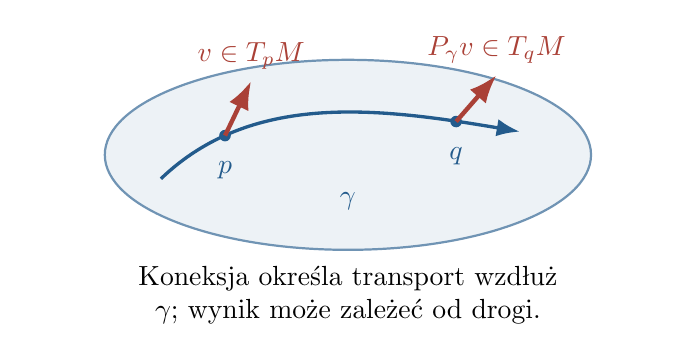
\begin{tikzpicture}[scale=0.95,>=Latex]
  \fill[manifoldblue!8] (0,0) ellipse (3.25 and 1.27);
  \draw[manifoldblue!65,thick] (0,0) ellipse (3.25 and 1.27);
  \draw[manifoldblue,very thick,->] (-2.5,-.32) .. controls (-1.3,.83) and (.36,.64) .. (2.30,.31);
  \path (-2.5,-.32) .. controls (-1.3,.83) and (.36,.64) .. (2.30,.31)
       coordinate[pos=.22] (pa) coordinate[pos=.85] (qa);
  \fill[manifoldblue] (pa) circle (2.2pt) node[below=6pt] {$p$};
  \fill[manifoldblue] (qa) circle (2.2pt) node[below=6pt] {$q$};
  \draw[manifoldred,ultra thick,->] (pa) -- ++(.35,.73) node[above] {$v\in T_pM$};
  \draw[manifoldred,ultra thick,->] (qa) -- ++(.54,.62) node[above] {$P_\gamma v\in T_qM$};
  \node[manifoldblue] at (0,-.62) {$\gamma$};
  \node[align=center,text width=7.9cm,below] at (0,-1.36)
    {Koneksja określa transport wzdłuż $\gamma$; wynik może zależeć od drogi.};
\end{tikzpicture}
\caption{Schemat transportu wzdłuż drogi. Strzałki reprezentują wektory w różnych przestrzeniach stycznych; ich położenie na kartce nie wyznacza metryki ani wielkości obrotu.}
\label{fig:koneksja-transport-idea}
\end{figure}

\begin{definicja}[Koneksja afiniczna]
\index{koneksja afiniczna@Koneksja afiniczna}
\label{def:koneksja-afiniczna}
Koneksją afiniczną na $TM$ nazywamy przyporządkowanie
$(X,Y)\mapsto\nabla_XY$ pól wektorowych, liniowe
nad $\R$ w obu argumentach, takie że dla $f\in C^\infty(M)$
\begin{equation}\label{eq:koneksja-aksjomaty}
 \nabla_{fX}Y=f\nabla_XY,
 \qquad \nabla_X(fY)=X(f)Y+f\nabla_XY.
\end{equation}
Pierwszy wzór pozwoli wykazać, że $\nabla_XY$ w $p$ zależy
tylko od wektora $X_p$. Drugi jest regułą iloczynu:
zmienia się zarówno wielkość współczynnika $f$,
jak i samo pole $Y$.
\end{definicja}

\begin{lemat}[Lokalność koneksji]
\label{lem:koneksja-lokalnosc}
Wartość $(\nabla_XY)_p$ zależy tylko od ograniczeń $X,Y$
do dowolnego otoczenia $p$. Można więc stosować koneksję
do pól określonych jedynie na otwartym podzbiorze $M$.
W pierwszym argumencie wystarcza sama wartość $X_p$.
\end{lemat}
\begin{proof}
Jeśli pole $Z$ znika na otoczeniu $U$ punktu $p$, wybieramy
gładką funkcję $\chi$ o nośniku zawartym w $U$, równą $1$
w pobliżu $p$. Takie funkcje daje konstrukcja z
Sekcji~\ref{sec:formy-podzial-jednosci}. Ponieważ $\chi Z=0$,
aksjomaty koneksji dają
\[
 0=\nabla_{\chi Z}Y=\chi\nabla_ZY,\qquad
 0=\nabla_X(\chi Z)=X(\chi)Z+\chi\nabla_XZ.
\]
Po obliczeniu w $p$ otrzymujemy $(\nabla_ZY)_p=0$
i $(\nabla_XZ)_p=0$. Odejmowanie pól dowodzi lokalności.
Pole określone na $U$ mnożymy przez taką funkcję $\chi$
i przedłużamy zerem poza $U$; wynik obliczenia w $p$
nie zależy od przedłużenia. Te lokalne definicje sklejają się.
W lokalnej ramce $X=X^i\partial_i$ pierwsza reguła daje
$(\nabla_XY)_p=X^i(p)(\nabla_{\partial_i}Y)_p$,
co dowodzi ostatniego zdania. Drugi argument wymaga
także pierwszych pochodnych współczynników pola $Y$.
\end{proof}

\begin{stwierdzenie}[Współczynniki lokalne]
\label{prop:koneksja-lokalna}
W mapie $(x^1,\ldots,x^n)$ koneksję wyznaczają
funkcje $\Gamma^k_{ij}$, zwane symbolami Christoffela,
określone przez
\begin{equation}\label{eq:def-christoffel}
 \nabla_{\partial_i}\partial_j
   =\sum_k\Gamma^k_{ij}\partial_k.
\end{equation}
Dla $X=X^i\partial_i$ i $Y=Y^j\partial_j$ mamy
\begin{equation}\label{eq:koneksja-wspolrzedne}
 (\nabla_XY)^k=X^i\bigl(\partial_iY^k+
                         \Gamma^k_{ij}Y^j\bigr).
\end{equation}
W powtarzających się indeksach stosujemy sumowanie.
\end{stwierdzenie}
\begin{proof}
Z pierwszego aksjomatu
$\nabla_XY=X^i\nabla_{\partial_i}(Y^j\partial_j)$.
Z drugiego
$\nabla_{\partial_i}(Y^j\partial_j)
=(\partial_iY^j)\partial_j
 +Y^j\Gamma^k_{ij}\partial_k$.
Zbierając współczynniki przy $\partial_k$,
otrzymujemy podany wzór. I odwrotnie:
gładkie funkcje $\Gamma^k_{ij}$ w mapie definiują
tam koneksję przez ten wzór.
\end{proof}

\begin{uwaga}[Symbole nie są tensorem]
\label{uw:symbole-nie-tensor}
Przy zamianie współrzędnych $x=x(y)$ stosujemy
$\partial_{y^a}=(\partial x^i/\partial y^a)\partial_{x^i}$
oraz regułę iloczynu. Jeśli $B^i_a=\partial x^i/\partial y^a$,
to przed zmianą bazy w wyniku mamy
\[
 \nabla_{\partial_{y^a}}\partial_{y^b}
 =\bigl(B^i_a\partial_{x^i}B^k_b
       +B^i_aB^j_b\Gamma^k_{ij}\bigr)\partial_{x^k}.
\]
Pierwszy składnik to $\partial^2x^k/\partial y^a\partial y^b$.
Po zapisaniu $\partial_{x^k}=(\partial y^c/\partial x^k)
\partial_{y^c}$ otrzymujemy
\begin{equation}\label{eq:transformacja-christoffel}
 \widetilde\Gamma^c_{ab}
 =\frac{\partial y^c}{\partial x^k}
  \left(
   \frac{\partial x^i}{\partial y^a}
   \frac{\partial x^j}{\partial y^b}\Gamma^k_{ij}
   +\frac{\partial^2x^k}{\partial y^a\partial y^b}
  \right).
\end{equation}
Druga pochodna jest dodatkowym składnikiem;
same $\Gamma^k_{ij}$ nie tworzą tensora.
To pozwala mieć zerowe symbole w kartezjańskim
opisie płaszczyzny i niezerowe w biegunowym,
choć geometrycznie jest to ta sama płaszczyzna.
\end{uwaga}

\begin{definicja}[Torsja i zgodność z metryką]
\index{torsja i zgodnosc z metryka@Torsja i zgodność z metryką}
\label{def:torsja-koneksja}
Torsją koneksji jest pole tensorowe
\[
 T(X,Y)=\nabla_XY-\nabla_YX-[X,Y].
\]
Koneksja jest \emph{bez torsji}, gdy $T=0$.
Jeżeli $g$ jest metryką, koneksja jest z nią
\emph{zgodna}, gdy dla dowolnych pól
\begin{equation}\label{eq:zgodnosc-metryczna}
 X\bigl(g(Y,Z)\bigr)
 =g(\nabla_XY,Z)+g(Y,\nabla_XZ).
\end{equation}
\end{definicja}

\begin{stwierdzenie}[Co zależy tylko od wartości w punkcie?]
\label{prop:torsja-tensor-roznica}
Torsja jest tensorem typu $(1,2)$. Jeżeli
$\nabla$ i $\widehat\nabla$ są koneksjami,
to $A(X,Y)=\widehat\nabla_XY-\nabla_XY$
również jest tensorem typu $(1,2)$.
\end{stwierdzenie}
\begin{proof}
W pierwszym argumencie dla torsji używamy
$[fX,Y]=f[X,Y]-Y(f)X$. Po rozwinięciu
\[
 T(fX,Y)=f\nabla_XY-Y(f)X-f\nabla_YX
          -f[X,Y]+Y(f)X=fT(X,Y).
\]
Analogicznie $[X,fY]=f[X,Y]+X(f)Y$,
więc wyrazy $X(f)Y$ w $T(X,fY)$ się skracają.
Ponieważ $\nabla$ i $\widehat\nabla$ mają tę
samą regułę iloczynu, również w ich różnicy
kasują się składniki $X(f)Y$.
To wyjaśnia, czemu przestrzeń wszystkich koneksji
jest afiniczna: do jednej koneksji można dodać
dowolny tensor takiego typu. W mapie
$T^k_{ij}=\Gamma^k_{ij}-\Gamma^k_{ji}$,
bo $[\partial_i,\partial_j]=0$.
\end{proof}

\section{Koneksja Leviego-Civity i wzór Koszula}
\label{sec:levi-civita-koszul}

Metryka dostarcza iloczynu skalarnego w każdym
punkcie. Wybieramy koneksję, która zachowuje ten
iloczyn podczas przemieszczania się, i żądamy
zerowej torsji. Te dwa warunki usuwają dowolność.

\begin{twierdzenie}[Istnienie i jednoznaczność koneksji Leviego-Civity]
\label{thm:levi-civita}
Każda metryka riemannowska $g$ na $M$ wyznacza
dokładnie jedną koneksję $\nabla$ zgodną z $g$
i bez torsji. Ta sama teza zachodzi dla metryki
pseudoriemannowskiej, w szczególności
Schwarzschilda i Kerra.
\end{twierdzenie}
\begin{proof}
\emph{Krok 1: wyprowadzenie wzoru i jednoznaczność.}
Załóżmy, że taka koneksja istnieje. Zapiszmy
\eqref{eq:zgodnosc-metryczna} kolejno dla
$(X,Y,Z)$, $(Y,Z,X)$ oraz $(Z,X,Y)$:
\begin{align*}
 Xg(Y,Z)&=g(\nabla_XY,Z)+g(Y,\nabla_XZ),\\
 Yg(Z,X)&=g(\nabla_YZ,X)+g(Z,\nabla_YX),\\
 Zg(X,Y)&=g(\nabla_ZX,Y)+g(X,\nabla_ZY).
\end{align*}
Dodajemy dwa pierwsze równania i odejmujemy
trzecie. Brak torsji daje
$\nabla_YX=\nabla_XY-[X,Y]$,
$\nabla_ZX=\nabla_XZ-[X,Z]$ oraz
$\nabla_ZY=\nabla_YZ-[Y,Z]$.
Po podstawieniu pary z $\nabla_XZ$ i pary
z $\nabla_YZ$ się skracają. Zostaje
\begin{align}\label{eq:koszul}
2g(\nabla_XY,Z)={}&Xg(Y,Z)+Yg(Z,X)-Zg(X,Y)\notag\\
 &+g([X,Y],Z)-g([X,Z],Y)-g([Y,Z],X).
\end{align}
Jest to \emph{wzór Koszula}. Jego prawa strona
zależy wyłącznie od $g,X,Y,Z$. Niezdegenerowanie
$g_p$ sprawia, że wartości $g_p(W,Z_p)$ dla
wszystkich $Z_p$ wyznaczają jedyny wektor $W$.
Stąd co najwyżej jedna taka koneksja.

\emph{Krok 2: konstrukcja.} Oznaczmy prawą stronę
\eqref{eq:koszul} przez $K(X,Y,Z)$ i zdefiniujmy
$\nabla_XY$ przez $2g(\nabla_XY,Z)=K(X,Y,Z)$.
Najpierw trzeba sprawdzić, że prawa strona
jest $C^\infty$-liniowa względem $Z$.
Po zastąpieniu $Z$ przez $fZ$ składniki z
$X(f)g(Y,Z)$ pochodzące od
$Xg(Y,fZ)$ i $-g([X,fZ],Y)$ mają przeciwne znaki;
tak samo znoszą się $Y(f)g(X,Z)$ z
$Yg(fZ,X)$ i $-g([Y,fZ],X)$.
Reszta jest pomnożona przez $f$.
Zatem $K(X,Y,\cdot)$ jest gładką $1$-formą,
której współczynniki w mapie to $K(X,Y,\partial_i)$.
Jawnie
\[
 (\nabla_XY)^j=\tfrac12g^{ji}K(X,Y,\partial_i).
\]
Macierz $G^{-1}$ jest gładka, więc otrzymujemy gładkie pole.
Definicje w różnych mapach są zgodne, ponieważ wszystkie
spełniają tę samą równość z $g$, a niezdegenerowanie
metryki zapewnia punktową jednoznaczność.

Sprawdźmy aksjomaty koneksji. W $K(fX,Y,Z)$
dodatkowe $Y(f)g(X,Z)$ z $Yg(Z,fX)$
znosi $-Y(f)g(X,Z)$ z $g([fX,Y],Z)$.
Dodatkowe $-Z(f)g(X,Y)$ z $-Zg(fX,Y)$
znosi $+Z(f)g(X,Y)$ z $-g([fX,Z],Y)$.
Wobec tego $K(fX,Y,Z)=fK(X,Y,Z)$.
W $K(X,fY,Z)$ dwukrotnie pojawia się
$X(f)g(Y,Z)$: z $Xg(fY,Z)$ oraz
$g([X,fY],Z)$. Wyrazy $Z(f)g(X,Y)$
z $-Zg(X,fY)$ i $-g([fY,Z],X)$
znoszą się. Dostajemy
\[
 K(X,fY,Z)=fK(X,Y,Z)+2X(f)g(Y,Z).
\]
Po podzieleniu przez $2$ i użyciu
niezdegenerowania $g$ są to dokładnie
aksjomaty \eqref{eq:koneksja-aksjomaty}.

\emph{Krok 3: sprawdzenie warunków.}
Różnica $K(X,Y,Z)-K(Y,X,Z)$ jest równa
$2g([X,Y],Z)$: pochodne metryki
się kasują, a antysymetria nawiasu daje
wyraz podwojony. Stąd
$\nabla_XY-\nabla_YX=[X,Y]$.
Dodając $K(X,Y,Z)$ i $K(X,Z,Y)$,
otrzymujemy $2Xg(Y,Z)$: pozostałe pochodne
i wyrazy z nawiasami redukują się parami.
To jest \eqref{eq:zgodnosc-metryczna}.
Użyliśmy jedynie niezdegenerowania macierzy $G$,
nie jej dodatniej określoności; dowód dotyczy
również metryk lorentzowskich.
\end{proof}

W szczególności istnienie metryki riemannowskiej
z Twierdzenia~\ref{thm:istnienie-metryki}
zapewnia istnienie \emph{jakiejś} koneksji
afinicznej na każdej rozmaitości z naszych założeń.
Koneksji jest zwykle wiele, ale dla ustalonego $g$
warunki z twierdzenia wybierają jedną.

\begin{stwierdzenie}[Podrozmaitość w przestrzeni euklidesowej]
\label{prop:koneksja-projekcja}
Jeżeli $M\subset\R^N$ ma metrykę indukowaną,
to jej koneksja Leviego-Civity jest równa
\[
 \nabla_XY=\operatorname{pr}_{TM}(D_XY),
\]
gdzie $D_XY$ oznacza zwykłą pochodną pola $Y$
traktowanego jako odwzorowanie do $\R^N$.
\end{stwierdzenie}
\begin{proof}
Rzut ortogonalny jest liniowy w punkcie,
a pochodna euklidesowa spełnia regułę iloczynu,
więc wzór określa koneksję. Pochodna iloczynu
skalarnego w $\R^N$ daje
$X\langle Y,Z\rangle
=\langle D_XY,Z\rangle+\langle Y,D_XZ\rangle$.
Składowe normalne obu pochodnych są prostopadłe
do $Y$ lub $Z$ i znikają z tej równości;
koneksja jest zgodna z metryką indukowaną.
Ponadto w lokalnej parametryzacji mieszane
pochodne drugiego rzędu komutują, więc
$D_XY-D_YX=[X,Y]$; po rzucie otrzymujemy
zerową torsję. Stosujemy Twierdzenie~\ref{thm:levi-civita}.
\end{proof}

\section{Symbole Christoffela w geometriach modelowych}
\label{sec:christoffel-przyklady}

W mapie pola bazowe komutują, więc wzór Koszula
z $X=\partial_i$, $Y=\partial_j$, $Z=\partial_\ell$
przyjmuje postać
\[
 2g_{k\ell}\Gamma^k_{ij}
 =\partial_i g_{j\ell}+\partial_j g_{i\ell}
    -\partial_\ell g_{ij}.
\]
Mnożymy przez $g^{m\ell}$, gdzie
$(g^{m\ell})=G^{-1}$. Ponieważ
$g^{m\ell}g_{k\ell}=\delta^m_k$, otrzymujemy
\begin{equation}\label{eq:christoffel-metryka}
 \boxed{\displaystyle
 \Gamma^m_{ij}=\frac12 g^{m\ell}
  (\partial_i g_{j\ell}+\partial_j g_{i\ell}
                         -\partial_\ell g_{ij}).}
\end{equation}
Algorytm jest prosty: zapisać $G$, odwrócić ją,
obliczyć pochodne współczynników, podstawić.
Duże metryki nie wymagają zapamiętania wielkiej
listy symboli; zwykle liczymy tylko te, które
potrzebne są w danym równaniu.

\begin{przyklad}[Płaszczyzna euklidesowa w dwóch mapach]
\label{prz:christoffel-biegunowe}
W kartezjańskiej mapie $g=\dd x^2+\dd y^2$,
wszystkie $g_{ij}$ są stałe, zatem $\Gamma^k_{ij}=0$.
W biegunowej mapie $x=r\cos\phi$, $y=r\sin\phi$
(dla $r>0$ i $\phi$ w otwartym przedziale długości co najwyżej
$2\pi$) ta sama metryka jest
$g=\dd r^2+r^2\dd\phi^2$.
Macierze $G=\operatorname{diag}(1,r^2)$
i $G^{-1}=\operatorname{diag}(1,r^{-2})$ oraz
$\partial_r g_{\phi\phi}=2r$ dają
\begin{equation}\label{eq:gamma-biegunowe}
 \Gamma^r_{\phi\phi}=-r,
 \qquad \Gamma^\phi_{r\phi}
 =\Gamma^\phi_{\phi r}=\frac1r,
\end{equation}
a wszystkie pozostałe symbole są zerowe.
Na przykład
$\nabla_{\partial_\phi}\partial_\phi=-r\partial_r$:
wektor $\partial_\phi$ w miarę obrotu układu
zmienia kierunek nawet wtedy, gdy płaszczyzna
pozostaje płaska. Wzór $\nabla_XY$ uwzględnia
ten obrót bazy.
\end{przyklad}

\begin{przyklad}[Sfera o promieniu $R$]
\label{prz:christoffel-sfera}
Z \eqref{eq:metryka-sfery} odczytujemy
$G=\operatorname{diag}(R^2,R^2\sin^2\theta)$.
Jedyna niezerowa pochodna współczynników to
$\partial_\theta g_{\phi\phi}
=2R^2\sin\theta\cos\theta$. Stąd
\begin{equation}\label{eq:gamma-sfera}
 \Gamma^\theta_{\phi\phi}
   =-\sin\theta\cos\theta,
 \qquad
 \Gamma^\phi_{\theta\phi}
 =\Gamma^\phi_{\phi\theta}=\cot\theta.
\end{equation}
Brak $R$ w tych symbolach jest zgodny z tym,
że stałe przemnożenie metryki nie zmienia
jej koneksji. Bieguny wymagają innej mapy;
$\cot\theta$ nie opisuje tam osobliwości sfery.
\end{przyklad}

\begin{przyklad}[Górna półprzestrzeń hiperboliczna]
\label{prz:christoffel-hiperboliczna}
Dla dwuwymiarowego modelu
$g=y^{-2}(\dd x^2+\dd y^2)$, $y>0$,
macierze $G=y^{-2}I$, $G^{-1}=y^2I$.
Ponieważ $\partial_y(y^{-2})=-2y^{-3}$,
\eqref{eq:christoffel-metryka} daje
\begin{equation}\label{eq:gamma-hiperboliczna}
 \Gamma^y_{xx}=\frac1y,\quad
 \Gamma^y_{yy}=-\frac1y,\quad
 \Gamma^x_{xy}=\Gamma^x_{yx}=-\frac1y.
\end{equation}
W wyższych wymiarach, dla $g=y^{-2}
(\sum_a\dd x_a^2+\dd y^2)$, podobnie
$\Gamma^y_{x_ax_b}=\delta_{ab}/y$,
$\Gamma^{x_a}_{x_by}=\Gamma^{x_a}_{yx_b}=-\delta^a_b/y$
oraz $\Gamma^y_{yy}=-1/y$; pozostałe symbole są zerowe.
Na przykład pole w kierunku $x$ przenoszone
pionowo musi mieć odpowiednio zmienne
współrzędne: $\nabla_{\partial_y}(y\partial_x)=0$.
Rzeczywiście $\partial_y(y)=1$ oraz
$\Gamma^x_{yx}y=-1$; jego długość w metryce
hiperbolicznej stale wynosi $1$.
\end{przyklad}

\begin{przyklad}[Kula Poincarégo: jawne symbole]
\label{prz:christoffel-dysk}
Metryka~\eqref{eq:hip-kula} ma postać
$g=\lambda(u)^2\sum_i(\dd u^i)^2$,
$\lambda=2/(1-|u|^2)>0$. Indeksy $u_i=u^i$ w tym
przykładzie odnoszą się do współrzędnych euklidesowych;
nie oznaczają obniżenia indeksu metryką hiperboliczną.
Po wstawieniu
$g_{ij}=\lambda^2\delta_{ij}$ i
$g^{ij}=\lambda^{-2}\delta^{ij}$ do
\eqref{eq:christoffel-metryka} otrzymujemy
dla dowolnej metryki takiej postaci
\begin{equation}\label{eq:gamma-konforemne}
 \Gamma^k_{ij}=\delta^k_i\partial_j\log\lambda
 +\delta^k_j\partial_i\log\lambda
 -\delta_{ij}\partial_k\log\lambda.
\end{equation}
Rzeczywiście $\partial_i g_{j\ell}
=2\lambda(\partial_i\lambda)\delta_{j\ell}$;
kontrakcja z $\lambda^{-2}\delta^{k\ell}/2$
daje trzy pokazane wyrazy. Ponieważ
$\partial_k\log\lambda=2u_k/(1-|u|^2)$,
otrzymujemy \emph{jawnie}
\begin{equation}\label{eq:gamma-dysk}
 \boxed{\displaystyle
 \Gamma^k_{ij}=\frac{2}{1-|u|^2}
   \bigl(\delta^k_i u_j+\delta^k_j u_i
                          -\delta_{ij}u_k\bigr).}
\end{equation}
Na przykład w dysku o współrzędnych $(u,v)$,
przy $D=1-u^2-v^2$, niezależne składowe to
\[
 \begin{array}{lll}
 \Gamma^u_{uu}=2u/D,&\Gamma^u_{uv}=2v/D,&
 \Gamma^u_{vv}=-2u/D,\\
 \Gamma^v_{uu}=-2v/D,&\Gamma^v_{uv}=2u/D,&
 \Gamma^v_{vv}=2v/D.
 \end{array}
\]
Wszystkie symbole znikają \emph{w środku} dysku,
ale to nie czyni metryki płaską: pochodne symboli
w~\eqref{eq:riemann-wspolrzedne} z
Rozdziału~\ref{ch:krzywizna} mogą być niezerowe.
Jako kontrolę wzoru weźmy średnicę $u=r$, $v=0$.
Pole $V=\frac{1-r^2}{2}\partial_v$ wzdłuż niej
ma długość $1$ i jest równoległe, gdyż
\[
 \nabla_{\partial_r}V
 =\left(-r+\Gamma^v_{uv}\frac{1-r^2}{2}\right)
             \partial_v
 =\left(-r+\frac{2r}{1-r^2}\frac{1-r^2}{2}\right)
             \partial_v=0.
\]
\end{przyklad}

\begin{przyklad}[Hiperboloida: symbole w mapie przestrzennej]
\label{prz:christoffel-hiperboloida}
Użyjmy współrzędnych $z$ z
\eqref{eq:hiperboloida-wspolrzedne-metryka},
oznaczając $t^2=1+|z|^2$. Także tutaj $z_i=z^i$
oznacza współrzędne w euklidesowej przestrzeni parametrów. Mamy
$g_{ij}=\delta_{ij}-z_i z_j/t^2$
oraz $g^{ij}=\delta^{ij}+z_i z_j$ z
\eqref{eq:hiperboloida-macierz-odwrotna}.
Po zróżniczkowaniu
\[
 \partial_i g_{j\ell}
 =-\frac{\delta_{ij}z_\ell+\delta_{i\ell}z_j}{t^2}
   +\frac{2z_i z_j z_\ell}{t^4},
\]
więc trzy pochodne ze wzoru
\eqref{eq:christoffel-metryka} łączą się w
\[
 \partial_i g_{j\ell}+\partial_j g_{i\ell}
                -\partial_\ell g_{ij}
 =-\frac{2z_\ell}{t^2}
            \left(\delta_{ij}-\frac{z_i z_j}{t^2}\right)
 =-\frac{2z_\ell}{t^2}g_{ij}.
\]
Ponieważ $g^{k\ell}z_\ell=t^2 z^k$, otrzymujemy
\begin{equation}\label{eq:gamma-hiperboloida}
 \boxed{\displaystyle\Gamma^k_{ij}=-z^k g_{ij}
  =-z^k\left(\delta_{ij}-\frac{z_i z_j}{1+|z|^2}\right).}
\end{equation}
Na przykład dla $z(\tau)=(\sinh\tau,0,\ldots,0)$
mamy $g_{11}=1/\cosh^2\tau$ oraz
$\Gamma^1_{11}=-\sinh\tau/\cosh^2\tau$.
Równanie geodezyjnej w pierwszej współrzędnej
przyjmuje zatem postać
$\ddot z^1+\Gamma^1_{11}(\dot z^1)^2
=\sinh\tau-\sinh\tau=0$,
zgodnie ze wzorem~\eqref{eq:exp-hiperboloida}
w rozdziale o geodezyjnych.
\end{przyklad}

Izometrie między modelami z
Przykładu~\ref{prz:trzy-modele-hiperboliczne}
przenoszą te koneksje: wynika to z jednoznaczności
koneksji Leviego-Civity przy zachowaniu zgodności
z metryką i braku torsji. Dokładniej, dla izometrii
$F:(M,g)\to(N,h)$ definiujemy na $M$
\[
 \widehat\nabla_XY=(F^{-1})_*
       \bigl(\nabla^h_{F_*X}(F_*Y)\bigr).
\]
Reguła łańcuchowa daje aksjomaty koneksji. Równości
$F_*[X,Y]=[F_*X,F_*Y]$ i $F^*h=g$ zapewniają zerową
torsję oraz zgodność z $g$. Jednoznaczność daje
$\widehat\nabla=\nabla^g$, czyli
$F_*(\nabla^g_XY)=\nabla^h_{F_*X}(F_*Y)$.
Symboli Christoffela
\emph{nie porównujemy bezpośrednio} między różnymi
mapami: transformują się wraz z pochodnymi zmiany
współrzędnych, podczas gdy sama koneksja jest
tym samym obiektem geometrycznym.

\begin{stwierdzenie}[Dywergencja zapisana przez koneksję]
\label{prop:dywergencja-koneksja}
Dla koneksji Leviego-Civity i pola $X$ na rozmaitości
riemannowskiej tensor $\nabla X$ przyporządkowuje wektorowi
$Y_p$ wektor $(\nabla_YX)_p$. Jego ślad jest dywergencją:
\begin{equation}\label{eq:dywergencja-koneksja}
 \operatorname{div}_gX=\nabla_iX^i
 =\partial_iX^i+\Gamma^i_{ij}X^j
 =\frac1{\sqrt{\det G}}\partial_i
       (\sqrt{\det G}\,X^i).
\end{equation}
Jest to ten sam operator, który wystąpił
w Twierdzeniu Gaussa w Rozdziale~\ref{ch:metryka-riemannowska}.
\end{stwierdzenie}
\begin{proof}
Podstawiamy \eqref{eq:christoffel-metryka}
i korzystamy z symetrii macierzy. Przy sumowaniu
po $i$ składniki
$g^{i\ell}\partial_i g_{j\ell}$
i $-g^{i\ell}\partial_\ell g_{ij}$ są przeciwne
po zamianie nazw indeksów $i,\ell$.
Pozostaje
\[
 \Gamma^i_{ij}=\tfrac12g^{i\ell}\partial_jg_{i\ell}
 =\partial_j\log\sqrt{\det G}.
\]
Ostatnia równość jest wzorem na pochodną
wyznacznika: $\partial_j\det G
=(\det G)\operatorname{tr}(G^{-1}\partial_jG)$.
Reguła iloczynu daje ostatnie wyrażenie
w \eqref{eq:dywergencja-koneksja}, zgodne
z wcześniejszym \eqref{eq:dywergencja-lokalna}.
\end{proof}

\section{Pochodna kowariantna i transport wzdłuż krzywej}
\label{sec:transport-rownolegly}

Pochodna $\nabla_XY$ odpowiada na pytanie:
jak szybko zmienia się $Y$, gdy ruszamy z punktu
w kierunku $X$, \emph{z uwzględnieniem zmiany lokalnej bazy}?
Wzór~\eqref{eq:koneksja-wspolrzedne} dodaje do
pochodnej współrzędnych dokładnie poprawkę
$\Gamma^k_{ij}X^iY^j$.

\begin{definicja}[Pochodna wzdłuż krzywej]
\index{pochodna wzdluz krzywej@Pochodna wzdłuż krzywej}
\label{def:pochodna-wzdluz-krzywej}
Niech $\gamma:I\to M$ będzie gładką krzywą.
Gładkie pole wzdłuż niej to gładkie odwzorowanie
$V:I\to TM$ z $V(t)\in T_{\gamma(t)}M$,
czyli gładki przekrój wiązki $\gamma^*TM$.
Jego pochodną kowariantną oznaczamy
$D V/\dd t$ lub $\nabla_{\dot\gamma}V$.
W mapie, przy $\gamma(t)=(x^i(t))$ oraz
$V(t)=V^k(t)\partial_k|_{\gamma(t)}$, jest to
\begin{equation}\label{eq:pochodna-kowariantna-krzywa}
 \frac{D V}{\dd t}
 =\left(\frac{\dd V^k}{\dd t}
   +\Gamma^k_{ij}(\gamma(t))\dot x^i V^j\right)
    \partial_k\big|_{\gamma(t)}.
\end{equation}
Pole jest \emph{równoległe} wzdłuż $\gamma$,
gdy $DV/\dd t=0$. Rozwiązanie z wartością
$V(a)=v$ oznaczymy przez $V(t)=P_{\gamma,a\to t}v$.
\end{definicja}

Uzasadnijmy niezależność od mapy bez zakładania, że $V$
ma przedłużenie do pola na $M$. Niech $J(t)$ będzie macierzą
$\partial y/\partial x$ w $\gamma(t)$ i niech
$A^k{}_j=\Gamma^k_{ij}(\gamma(t))\dot x^i$.
Współczynniki pola w nowych współrzędnych to
$\widetilde V=JV$. Wzór~\eqref{eq:transformacja-christoffel}
i pochodna $J^{-1}$ dają
\[
 \widetilde A=JAJ^{-1}-\dot J J^{-1},\qquad
 \frac{\dd\widetilde V}{\dd t}+\widetilde A\widetilde V
   =J\left(\frac{\dd V}{\dd t}+AV\right).
\]
Jest to dokładnie prawo transformacji wektora, więc definicja
jest poprawna również przy samoprzecięciach i punktach
z $\dot\gamma=0$. Potrzeba tego argumentu: dla krzywej
stałej $\gamma(t)=p$ pole $V(t)=t v$, $v\ne0$, nie jest
nawet lokalnie ograniczeniem jednego pola na $M$.

Jeżeli $V=Y\circ\gamma$ pochodzi od pola z otoczenia,
reguła łańcuchowa daje $DV/\dd t=\nabla_{\dot\gamma}Y$.
Dla dowolnego pola wzdłuż krzywej mamy też
$D(fV)/\dd t=f'V+f\,DV/\dd t$. Przy zmianie parametru
$t=h(s)$ bezpośrednie podstawienie do wzoru daje
\begin{equation}\label{eq:transport-reparametryzacja}
 \frac{D(V\circ h)}{\dd s}
   =h'(s)\frac{DV}{\dd t}\bigg|_{t=h(s)}.
\end{equation}
W szczególności zachowująca orientację gładka zmiana
parametru nie zmienia transportu między końcami.

\begin{twierdzenie}[Istnienie i własności transportu]
\label{thm:transport-rownolegly}
Dla gładkiej krzywej $\gamma:[a,b]\to M$
i $v\in T_{\gamma(a)}M$ istnieje dokładnie
jedno równoległe pole $V$ wzdłuż $\gamma$
spełniające $V(a)=v$. Transport
$P_{\gamma,a\to b}:T_{\gamma(a)}M\to T_{\gamma(b)}M$
jest liniowym izomorfizmem. Na kolejnych
odcinkach drogi transporty składają się;
po odwróceniu drogi otrzymujemy odwrotność.
Jeżeli koneksja jest zgodna z metryką $g$, to
\begin{equation}\label{eq:transport-izometria}
 g_{\gamma(t)}(P_{a\to t}v,P_{a\to t}w)
   =g_{\gamma(a)}(v,w).
\end{equation}
Dotyczy to również metryk lorentzowskich,
gdzie zachowywana forma nie jest dodatnio określona.
\end{twierdzenie}
\begin{proof}
W jednej mapie warunek $DV/\dd t=0$
jest liniowym układem zwyczajnych równań
różniczkowych
\begin{equation}\label{eq:ode-transport}
 \dot V^k(t)=-A^k{}_j(t)V^j(t),\qquad
 A^k{}_j(t)=\Gamma^k_{ij}(\gamma(t))\dot x^i(t).
\end{equation}
Współczynniki są ciągłe. Twierdzenie o liniowym
układzie ODE daje jednoznaczne rozwiązanie na
każdym zwartym odcinku, na którym krzywa
pozostaje w mapie: rozwiązanie nie może uciec
do nieskończoności w skończonym czasie przy
ciągłej, ograniczonej macierzy $A(t)$. Istotnie, równanie
całkowe i nierówność Grönwalla dają, dla $t\ge t_0$,
\[
 |V(t)|\le |V(t_0)|
       \exp\!\left(\int_{t_0}^t\|A(u)\|\,\dd u\right).
\]
Ograniczoność $A$ i $V$ ogranicza też $\dot V=-AV$,
więc na skończonym końcu przedziału istnieje granica $V$;
lokalne twierdzenie o istnieniu przedłuża rozwiązanie.
Ten sam argument działa wstecz w czasie.
Zwartość $[a,b]$ pozwala podzielić go na
skończenie wiele odcinków, z których każdy
mieści się w jednej mapie. Rozwiązania sklejamy
zgodnie z ich jednoznacznością na przecięciach.

Liniowość układu w $V$ daje liniowość transportu.
Rozwiązując równanie od $b$ ku $a$, dostajemy
odwrotność; jednoznaczność daje też prawo
składania po przecięciu drogi. Wreszcie
zgodność metryczna w lokalnej bazie ma postać
$\partial_i g_{jk}=\Gamma^\ell_{ij}g_{\ell k}
+\Gamma^\ell_{ik}g_{j\ell}$. Różniczkując
$g_{jk}(\gamma(t))V^j(t)W^k(t)$, dostajemy więc,
także bez przedłużania $V,W$ poza krzywą,
\[
 \frac{\dd}{\dd t}g(V,W)
 =g(DV/\dd t,W)+g(V,DW/\dd t).
\]
Gdy $V,W$ są równoległe, prawa strona jest
zerem, więc iloczyn pozostaje stały.
\end{proof}

Dla ciągłej krzywej kawałkami gładkiej, z podziałem na
skończenie wiele gładkich odcinków, definiujemy transport
jako złożenie transportów na tych odcinkach. Jednoznaczność
zapewnia niezależność od zagęszczenia podziału. W ten sposób
prawo składania obejmuje również sklejenia z narożnikiem.

Transport zależy zwykle od \emph{drogi}, a nie
tylko od jej końców. Jeśli koneksja jest zgodna z metryką
i krzywa jest zamknięta, jej transport jest izometrią
$T_pM\to T_pM$;
poniższy przykład pokaże niezerowy obrót
wektora po pełnym okrążeniu.

\begin{przyklad}[Obrót po równoleżniku sfery]
\label{prz:transport-sfera}
Na sferze $S_R^2$, $R>0$, użyjmy lokalnie współrzędnych
$(\theta,\phi)$ i ramki ortonormalnej
\[
 e_\theta=R^{-1}\partial_\theta,
 \qquad e_\phi=(R\sin\theta)^{-1}\partial_\phi.
\]
Idźmy po równoleżniku $\theta=\theta_0$,
$\phi$ od $0$ do $2\pi$, z $0<\theta_0<\pi$.
Cały równoleżnik nie mieści się w jednej mapie kątowej,
ale pola $e_\theta,e_\phi$ sklejają się do gładkiej ramki
na sferze bez biegunów i są $2\pi$-okresowe w $\phi$.
Możemy zatem rozwiązać równanie na całym przedziale.
Wstawiając \eqref{eq:gamma-sfera} do reguły
iloczynu, otrzymujemy
\[
 \nabla_{\partial_\phi}e_\theta
   =\cos\theta_0\,e_\phi,
 \qquad
 \nabla_{\partial_\phi}e_\phi
   =-\cos\theta_0\,e_\theta.
\]
Jeśli $V=A(\phi)e_\theta+B(\phi)e_\phi$,
to równanie $DV/\dd\phi=0$ ma postać
\[
 A'=B\cos\theta_0,
 \qquad B'=-A\cos\theta_0,
 \quad\Longrightarrow\quad
 A+iB=(A(0)+iB(0))e^{-i\phi\cos\theta_0}.
\]
Po powrocie do punktu początkowego ramka
jest znowu ta sama, a wektor obrócił się
o kąt $-2\pi\cos\theta_0$ modulo $2\pi$, mierzony od
$e_\theta$ ku $e_\phi$.
Na równiku kąt jest zerowy. Dla
$\theta_0=\pi/3$ wynosi $-\pi$: wektor
wraca przeciwnie skierowany. Obliczenie
pokazuje różnicę między przenoszeniem
\emph{równoległym na sferze} a utrzymywaniem
strzałki nieruchomej na kartce.
\end{przyklad}

\begin{figure}[htbp]
\centering
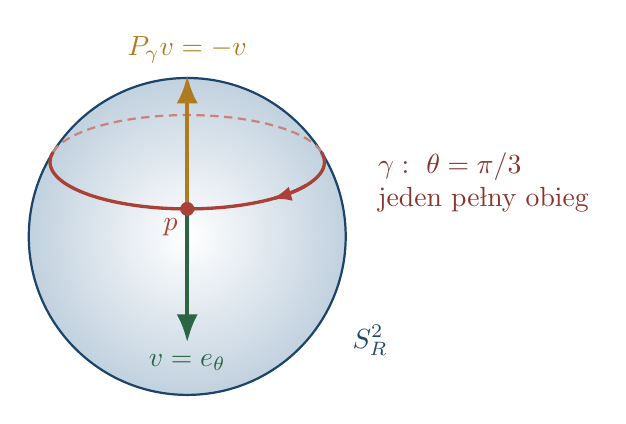
\begin{tikzpicture}[>=Latex,scale=1.15]
  % Rzut ortogonalny (X,Y,Z) -> (X, cos(20) Z - sin(20) Y).
  % R=1.75, theta=60 stopni; widoczność: Y cos(20)+Z sin(20)>=0.
  \pgfmathsetmacro{\latradius}{1.75*sin(60)}
  \pgfmathsetmacro{\latcenter}{1.75*cos(60)*cos(20)}
  \pgfmathsetmacro{\latheight}{\latradius*sin(20)}
  \pgfmathsetmacro{\limbangle}{asin(cot(60)*tan(20))}
  \pgfmathsetmacro{\pointheight}{\latcenter-\latheight}
  \shade[inner color=white,outer color=manifoldblue!28] (0,0) circle (1.75);
  \draw[manifoldblue!75!black,thick] (0,0) circle (1.75);
  \draw[manifoldred!65,densely dashed,thick]
    plot[domain=180+\limbangle:360-\limbangle,samples=70,variable=\u]
       ({\latradius*cos(\u)},{\latcenter-\latheight*sin(\u)});
  \draw[manifoldred,very thick]
    plot[domain=-\limbangle:180+\limbangle,samples=70,variable=\u]
       ({\latradius*cos(\u)},{\latcenter-\latheight*sin(\u)});
  \draw[manifoldred,very thick,-{Latex[length=2.5mm]}]
    plot[domain=30:52,samples=15,variable=\u]
       ({\latradius*cos(\u)},{\latcenter-\latheight*sin(\u)});
  \coordinate (p) at (0,\pointheight);
  \draw[manifoldgreen!80!black,ultra thick,->]
    (p) -- ++(0,{-1.5*sin(80)}) node[below] {$v=e_\theta$};
  \draw[manifoldgold!85!black,ultra thick,->]
    (p) -- ++(0,{1.5*sin(80)}) node[above] {$P_\gamma v=-v$};
  \fill[manifoldred] (p) circle (2.2pt) node[below left] {$p$};
  \node[manifoldblue!80!black] at (2.02,-1.15) {$S_R^2$};
  \node[manifoldred!80!black,align=left,anchor=west] at (2.0,.60)
    {$\gamma:\ \theta=\pi/3$\\jeden pełny obieg};
\end{tikzpicture}
\caption{Transport po równoleżniku $\theta=\pi/3$ obraca wektor
o $-\pi$. Dla czytelności początek pętli wybrano w punkcie
$p$ o $\phi=\pi/2$ (zakres parametru przesuwa się wtedy
o $\pi/2$). Strzałki są rzutami przeciwnych wektorów
w tej samej płaszczyźnie $T_pS_R^2$, narysowanymi w tej samej skali.
Przerywana część równoleżnika leży z tyłu sfery.}
\label{fig:transport-sfera}
\end{figure}

\subsection*{Pochodna kowariantna innych pól tensorowych}
\label{subsec:pochodna-kowariantna-tensory}
Pochodna funkcji to $\nabla_X f=X(f)$. Dla
$1$-formy $\alpha$ definiujemy $\nabla_X\alpha$
przez wymóg różniczkowania parowania:
\begin{equation}\label{eq:pochodna-kowariantna-forma}
 (\nabla_X\alpha)(Y)
  =X\bigl(\alpha(Y)\bigr)-\alpha(\nabla_XY).
\end{equation}
Prawa strona jest $C^\infty(M)$-liniowa w $Y$: po
zastąpieniu $Y$ przez $fY$ dwa składniki $X(f)\alpha(Y)$
znoszą się. Określa więc $1$-formę. W argumencie $X$
jest liniowa nad funkcjami, a w $\alpha$ spełnia regułę
Leibniza. We współrzędnych
$(\nabla_i\alpha)_j=\partial_i\alpha_j
-\Gamma^k_{ij}\alpha_k$. Na tensorach
definiujemy $\nabla_X$ przez regułę Leibniza
względem iloczynu tensorowego i zgodność
z kontrakcją (ściąganiem indeksów). Ściślej, dla tensora
$S$ typu $(r,s)$, $1$-form $\alpha_1,\ldots,\alpha_r$
i pól $Y_1,\ldots,Y_s$ wymagamy
\begin{align*}
 (\nabla_XS)(\alpha_1,\ldots,\alpha_r,Y_1,\ldots,Y_s)
 ={}&X\bigl(S(\alpha_1,\ldots,\alpha_r,Y_1,\ldots,Y_s)\bigr)\\
 &-\sum_{a=1}^r S(\alpha_1,\ldots,\nabla_X\alpha_a,\ldots,
                         \alpha_r,Y_1,\ldots,Y_s)\\
 &-\sum_{b=1}^s S(\alpha_1,\ldots,\alpha_r,
                         Y_1,\ldots,\nabla_XY_b,\ldots,Y_s).
\end{align*}
Reguły Leibniza sprawiają, że pochodne mnożników
w każdym argumencie się znoszą. Wynik jest więc tensorem
typu $(r,s)$, określonym bez wyboru bazy. Rozwinięcie
w lokalnych iloczynach tensorowych wektorów bazowych
i form dualnych dowodzi istnienia i jednoznaczności
rozszerzenia: każdy górny indeks wnosi składnik z $+\Gamma$,
a każdy dolny z $-\Gamma$. Na przykład
\[
 (\nabla_i S)_{jk}
 =\partial_iS_{jk}
  -\Gamma^\ell_{ij}S_{\ell k}
  -\Gamma^\ell_{ik}S_{j\ell}.
\]
Dla koneksji zgodnej z metryką dodatkowo $\nabla_i g_{jk}=0$;
jest to właśnie warunek~\eqref{eq:zgodnosc-metryczna}.
Dowolna koneksja afiniczna nie musi go spełniać.
W przypadku koneksji bez torsji pochodna Liego
z Rozdziału~\ref{ch:pola} i pochodna
kowariantna mają związek
\begin{equation}\label{eq:lie-koneksja}
 \Lie_XY=[X,Y]=\nabla_XY-\nabla_YX.
\end{equation}
Pochodna Liego porównuje pola przez przepływ
$X$, a pochodna kowariantna wykorzystuje
wybraną koneksję. Równość jest konsekwencją
zerowej torsji, nie definicją którejś z pochodnych.

\section{Przykłady w metrykach Schwarzschilda i Kerra}
\label{sec:koneksja-schwarzschild-kerr}

W obu czasoprzestrzeniach z Rozdziału~\ref{ch:metryka-riemannowska}
macierz metryki jest nieosobliwa w podanej tam
dziedzinie. Wzór Koszula daje zatem jednoznaczną
koneksję także tutaj. Transport zachowuje
\emph{lorentzowski iloczyn} wektorów;
nie interpretujemy $g(v,v)$ jako kwadratu
euklidesowej długości dla wszystkich wektorów.

\begin{przyklad}[Wybrane symbole Schwarzschilda]
\label{prz:koneksja-schwarzschild}
Niech $f(r)=1-2M/r$, zatem $f'(r)=2M/r^2$.
Dla metryki~\eqref{eq:schwarzschild}
macierz jest diagonalna:
\[
 (g_{\mu\nu})
 =\operatorname{diag}(-f,f^{-1},r^2,r^2\sin^2\theta),
 \qquad g^{rr}=f,\quad g^{tt}=-f^{-1}.
\]
Liczymy kilka przydatnych składników
za pomocą \eqref{eq:christoffel-metryka}:
\begin{align}\label{eq:gamma-schwarzschild}
 \Gamma^t_{tr}=\Gamma^t_{rt}
   &=\frac{f'}{2f}=\frac{M}{r^2f},
 &\Gamma^r_{tt}&=\frac{ff'}2=\frac{Mf}{r^2},\notag\\
 \Gamma^r_{rr}&=-\frac{f'}{2f},
 &\Gamma^r_{\theta\theta}&=-rf,
 &\Gamma^r_{\phi\phi}&=-rf\sin^2\theta,\\
 \Gamma^\theta_{r\theta}=\Gamma^\theta_{\theta r}
   &=\frac1r,
 &\Gamma^\phi_{r\phi}=\Gamma^\phi_{\phi r}&=\frac1r.
 \notag
\end{align}
Na przykład
$\Gamma^r_{tt}=-\tfrac12g^{rr}\partial_rg_{tt}
=-\tfrac12f(-f')=ff'/2$, a
$\Gamma^r_{\theta\theta}
=-\tfrac12 f\partial_r(r^2)=-rf$.
Pozostałe symbole kątowe są identyczne jak
w \eqref{eq:gamma-sfera}; pełny spis nie jest
potrzebny do użycia metody.

Dla drogi radialnej
$\gamma(s)=(t_0,r(s),\theta_0,\phi_0)$
wektor $V(s)=V^\theta(s)\partial_\theta$
jest równoległy wtedy i tylko wtedy, gdy
\[
 \frac{\dd V^\theta}{\dd s}
 +\frac{\dot r}{r}V^\theta=0,
 \qquad\Longleftrightarrow\qquad
 r(s)V^\theta(s)=\text{stała}.
\]
To łatwy test wzoru: $g_{\theta\theta}=r^2$,
więc $g(V,V)=r^2(V^\theta)^2$ jest zachowane.
Chodzi o transport w pełnej czasoprzestrzeni
wzdłuż tej wybranej drogi, nie o wyznaczenie
trajektorii fizycznej.
\end{przyklad}

\begin{przyklad}[Wybrane symbole Kerra]
\label{prz:koneksja-kerr}
Stosujemy $\Sigma=r^2+a^2\cos^2\theta$,
$\Delta=r^2-2Mr+a^2$ oraz współrzędne
Boyera--Lindquista z \eqref{eq:kerr}.
W bloku $(r,\theta)$ metryka i jej odwrotność
są diagonalne:
\[
 g_{rr}=\frac{\Sigma}{\Delta},\quad
 g_{\theta\theta}=\Sigma,\quad
 g^{rr}=\frac{\Delta}{\Sigma},\quad
 g^{\theta\theta}=\frac1\Sigma.
\]
Ponieważ $\partial_r\Sigma=2r$ oraz
$\partial_r\Delta=2(r-M)$, otrzymujemy
\begin{align}\label{eq:gamma-kerr-proste}
 \Gamma^r_{rr}
   &=\tfrac12g^{rr}\partial_rg_{rr}
     =\frac r\Sigma-\frac{r-M}{\Delta},
 & \Gamma^r_{\theta\theta}
   &=-\tfrac12g^{rr}\partial_rg_{\theta\theta}
     =-\frac{r\Delta}{\Sigma},\notag\\
 \Gamma^\theta_{r\theta}
  =\Gamma^\theta_{\theta r}&=\frac r\Sigma,
 &\Gamma^r_{r\theta}
  =\Gamma^r_{\theta r}
  &=-\frac{a^2\sin\theta\cos\theta}{\Sigma}.
\end{align}
Ostatni wzór pochodzi z
$\frac12 g^{rr}\partial_\theta g_{rr}
=\frac{\partial_\theta\Sigma}{2\Sigma}$.
Pokazuje, że współczynnik radialny może
zmieniać się także przy zmianie kąta $\theta$.

Parametr obrotu $a$ wprowadza sprzężenie
między czasem a kierunkiem $\phi$.
Z \eqref{eq:kerr} mamy
$g_{t\phi}=-2Mar\sin^2\theta/\Sigma$.
Metryka nie zależy od $t,\phi$ i nie ma
wyrazów $\dd r\,\dd t$ ani $\dd r\,\dd\phi$,
zatem \eqref{eq:christoffel-metryka} daje
\begin{align}\label{eq:gamma-kerr-mieszany}
 \Gamma^r_{t\phi}=\Gamma^r_{\phi t}
 &=-\frac12\frac\Delta\Sigma\partial_rg_{t\phi}
  =-\frac{Ma\Delta\sin^2\theta
                (r^2-a^2\cos^2\theta)}{\Sigma^3},\notag\\
 \partial_rg_{t\phi}
 &=\frac{2Ma\sin^2\theta
                (r^2-a^2\cos^2\theta)}{\Sigma^2}.
\end{align}
Przy $a=0$ składnik mieszany znika,
$\Sigma=r^2$, $\Delta=r^2f$;
\eqref{eq:gamma-kerr-proste} redukuje się
do radialnych i kątowych wzorów Schwarzschilda.
To sprawdzian rachunku oraz zależności obu metryk.
\end{przyklad}

Nie należy odczytywać pojedynczego symbolu
Christoffela jako niezależnej od współrzędnych
„siły”. Wzór~\eqref{eq:transformacja-christoffel}
zmienia jego wartość po zmianie mapy.
Geometryczny sens mają całe równania
transportu i pochodne kowariantne.

\section{Dlaczego koneksja pojawia się w równaniu ruchu?}
\label{sec:energia-koneksja}

Funkcjonał energii z \eqref{eq:dlugosc-energia}
pozwala rozpoznać krzywe stacjonarne.
W tej sekcji zakładamy $a<b$ i gładkość $\gamma$.
Rozpatrujemy rozmaitość bez brzegu albo krzywą zawartą
w jej wnętrzu, aby dopuszczalne były dowolne małe wariacje.
Dla ustalonych końców i lokalnego zapisu
$\gamma(t)=(x^i(t))$ mamy
\begin{equation}\label{eq:energia-lokalna-koneksja}
 E(\gamma)=\frac12\int_a^b
       g_{ij}(x(t))\dot x^i(t)\dot x^j(t)\,\dd t.
\end{equation}
Niech $x(t,s)$ będzie wariacją z końcami
niezależnymi od $s$ i
$\eta^k(t)=\partial_sx^k(t,s)|_{s=0}$.
Różniczkując pod całką i uwzględniając
symetrię $g_{ij}$, otrzymujemy
\[
 \left.\frac{\dd E}{\dd s}\right|_{s=0}
 =\int_a^b\left(
  \tfrac12\partial_k g_{ij}\,\eta^k\dot x^i\dot x^j
  +g_{kj}\dot\eta^k\dot x^j\right)\dd t.
\]
Całkując drugi składnik przez części,
wyraz brzegowy $[g_{kj}\eta^k\dot x^j]_a^b$
jest zerowy. Dostajemy
\[
 \delta E=\int_a^b\eta^k
 \left(\tfrac12\partial_k g_{ij}\dot x^i\dot x^j
      -\frac{\dd}{\dd t}(g_{kj}\dot x^j)\right)\dd t.
\]
Jeśli $\delta E=0$ dla wszystkich $\eta$
o zwartym nośniku we wnętrzu przedziału,
lemat podstawowy rachunku wariacyjnego
daje dla każdego $k$
\[
 g_{kj}\ddot x^j
 +\partial_i g_{kj}\dot x^i\dot x^j
 -\tfrac12\partial_k g_{ij}\dot x^i\dot x^j=0.
\]
Wyjaśnijmy dwa użyte tu kroki. Każde gładkie $\eta$ o
zwartym nośniku wewnątrz odcinka zawartego w mapie
realizuje wariacja $x(t,s)=x(t,0)+s\eta(t)$ dla małego
$|s|$, sklejona z niezmienioną krzywą poza tym odcinkiem.
Zwartość nośnika zapewnia, że pozostajemy w dziedzinie mapy.
Jeśli zaś ciągły współczynnik przy pewnym $\eta^k$ w całce
byłby dodatni (lub ujemny) w jednym punkcie, miałby ten sam
znak w małym otoczeniu. Nieujemna, niezerowa funkcja gładka
o nośniku w tym otoczeniu dawałaby niezerową całkę.
To dowód potrzebnej wersji lematu podstawowego.

Iloczyn $\dot x^i\dot x^j$ jest symetryczny;
zastępujemy więc $\partial_i g_{kj}$ przez
$\tfrac12(\partial_i g_{kj}+\partial_jg_{ki})$.
Po pomnożeniu przez $g^{\ell k}$ wzór
\eqref{eq:christoffel-metryka} daje
\begin{equation}\label{eq:rownanie-geodezyjnej-zapowiedz}
 \ddot x^\ell+\Gamma^\ell_{ij}\dot x^i\dot x^j=0,
 \qquad\text{czyli}\qquad
 \frac{D\dot\gamma}{\dd t}=0.
\end{equation}
Rachunek jest lokalny: wystarczy stosować takie wariacje
w kolejnych mapach pokrywających krzywą. Odwrotnie,
jeśli $D\dot\gamma/\dd t=0$, to dla dowolnej gładkiej
wariacji o ustalonych końcach całkowanie przez części
na odcinkach zawartych w mapach daje $\delta E=0$.
Wyrazy brzegowe w punktach podziału znoszą się, ponieważ
każdy jest wartością tego samego iloczynu
$g(\partial_s\gamma,\dot\gamma)$ z przeciwnymi znakami.
Stacjonarność jest więc równoważna temu równaniu.

Krzywa stacjonarna energii przenosi więc
swój wektor prędkości równolegle. Takie krzywe
nazywamy \emph{geodezyjnymi} z parametrem
afinicznym. Zgodność z metryką daje
$\frac{\dd}{\dd t}g(\dot\gamma,\dot\gamma)
=2g(D\dot\gamma/\dd t,\dot\gamma)=0$;
w przypadku riemannowskim prędkość ma zatem stałą normę.
Określenie parametru jest istotne: dla $\widetilde\gamma(s)
=\gamma(h(s))$ reguła~\eqref{eq:transport-reparametryzacja} daje
\[
 \frac{D\dot{\widetilde\gamma}}{\dd s}
 =h''(s)\dot\gamma(h(s))
       +(h'(s))^2\frac{D\dot\gamma}{\dd t}\bigg|_{t=h(s)}.
\]
Dla niestałej geodezyjnej $\dot\gamma$ nigdzie nie znika
(jest transportem niezerowego wektora), więc gładka
zmiana parametru zachowuje równanie dokładnie wtedy,
gdy $h(s)=cs+d$ z $c\ne0$.
Dalsze własności geodezyjnych i odwzorowanie
wykładnicze omówimy w następnym rozdziale,
a krzywiznę w dalszej części skryptu. Dla metryki lorentzowskiej
to samo równanie ma sens jako równanie
stacjonarności odpowiedniego działania;
nie twierdzimy, że definiuje odległość
riemannowską na czasoprzestrzeni.

\par\smallskip
{\footnotesize\noindent\emph{Dalsza lektura:}
\href{https://www.math.toronto.edu/mein/teaching/LectureNotes/rieall.pdf}
{Toronto} (koneksja i transport),
\href{https://web.mit.edu/8.962/www/lecnotes/8_962TA-lec-all.pdf}
{MIT} (symbole Schwarzschilda),
\href{https://sites.science.oregonstate.edu/coursewikis/GGR/book/content/kerr}
{Oregon} (metryka Kerra).\par}

\chapter{Geodezyjne, odwzorowanie wykładnicze i zupełność}
\label{ch:geodezyjne-exp}

W Rozdziale~\ref{ch:koneksje} otrzymaliśmy równanie
$D\dot\gamma/\dd t=0$ jako warunek stacjonarności
energii. Teraz wyjaśnimy, kiedy taka krzywa
rzeczywiście jest najkrótsza, jak opisuje otoczenie
punktu i co gwarantuje jej istnienie przez dowolnie
długi czas. Ostatnia część rozdziału odróżnia te
riemannowskie twierdzenia od geodezyjnych
czasoprzestrzeni Schwarzschilda i Kerra.

W całym rozdziale rozmaitości są gładkie i \emph{bez brzegu}.
Jeśli nie zaznaczono inaczej, metryka jest riemannowska;
odległości rozpatrujemy w jednej składowej spójnej.
Brak brzegu jest istotny: domknięty przedział z metryką
euklidesową jest zwarty, ale prosta dochodząca do jego
końca nie ma geodezyjnego przedłużenia w tym przedziale.

\section{Geodezyjna i pierwsza wariacja}
\label{sec:geodezyjna-pierwsza-wariacja}

\begin{definicja}[Geodezyjna]
\index{geodezyjna@Geodezyjna}
\label{def:geodezyjna}
Geodezyjną koneksji $\nabla$ nazywamy krzywą
$\gamma:I\to M$ spełniającą
\begin{equation}\label{eq:geodezyjna-ode}
 \nabla_{\dot\gamma}\dot\gamma=0,
 \qquad
 \ddot x^k+\Gamma^k_{ij}(x)\dot x^i\dot x^j=0.
\end{equation}
Użyty parametr jest \emph{afiniczny}.
Gdy $g$ jest metryką, mamy na myśli jej
koneksję Leviego-Civity.
\end{definicja}

Zgodność koneksji z metryką daje
$\frac{\dd}{\dd t}g(\dot\gamma,\dot\gamma)
=2g(D\dot\gamma/\dd t,\dot\gamma)=0$.
Wektor prędkości geodezyjnej riemannowskiej ma więc stałą
normę. Parametr $s=at+b$, $a\ne0$,
zachowuje równanie~\eqref{eq:geodezyjna-ode};
dowolna nieliniowa zmiana parametru na ogół
go nie zachowuje. Dla przykładu prosta
$\gamma(t)=p+tv$ w $\R^n$ jest geodezyjną,
ale dla $v\ne0$ krzywa $p+t^2v$ nie spełnia równania geodezyjnej
w parametrze $t$.

\begin{stwierdzenie}[Dane początkowe]
\label{prop:geodezyjna-dane-poczatkowe}
Dla każdego $p\in M$ i $v\in T_pM$ istnieje
jedyna maksymalna geodezyjna $\gamma_{p,v}$
o $\gamma_{p,v}(0)=p$, $\dot\gamma_{p,v}(0)=v$.
Jest określona co najmniej dla $|t|<\varepsilon$
zależnego od $(p,v)$ i zależy gładko od danych
tam, gdzie jest określona.
\end{stwierdzenie}
\begin{proof}
W mapie wprowadzamy $u^k=\dot x^k$.
Równanie drugiego rzędu staje się gładkim
układem pierwszego rzędu na otwartym
podzbiorze $\R^{2n}$:
\[
 \dot x^k=u^k,
 \qquad \dot u^k=-\Gamma^k_{ij}(x)u^iu^j.
\]
Twierdzenie Picarda--Lindelöfa o lokalnym
istnieniu, jednoznaczności i gładkiej zależności
od danych dla gładkiego pola na $TM$ daje
rozwiązanie. Jednoznaczność pozwala skleić
rozwiązania z różnych map i przedłużać je
do maksymalnego przedziału. Nie zakładamy
jeszcze, że tym przedziałem jest cała $\R$.
\end{proof}

Pierwsza wariacja jest dobrym miejscem na
rozróżnienie dwóch zdań: \emph{geodezyjna jest
punktem stacjonarnym długości} oraz
\emph{krótki jej fragment minimalizuje długość}.
Drugie wymaga osobnego dowodu poniżej.

\begin{twierdzenie}[Wzór na pierwszą wariację długości]
\label{thm:pierwsza-wariacja-dlugosci}
Niech $F(s,t)$ będzie gładką wariacją regularnej
krzywej $\gamma(t)=F(0,t)$, $t\in[a,b]$, $a<b$,
na rozmaitości riemannowskiej.
Oznaczmy $V=\partial_sF|_{s=0}$ i
$T=\dot\gamma/|\dot\gamma|_g$.
Wtedy
\begin{equation}\label{eq:pierwsza-wariacja-dlugosci}
 \left.\frac{\dd}{\dd s}L(F_s)\right|_{s=0}
  =\bigl[g(V,T)\bigr]_a^b
    -\int_a^b g\!\left(V,\frac{DT}{\dd t}\right)\dd t.
\end{equation}
Jeżeli $\gamma$ ma prędkość $1$, to
$T=\dot\gamma$ i $DT/\dd t=D\dot\gamma/\dd t$.
Przy ustalonych końcach składnik brzegowy znika.
\end{twierdzenie}
\begin{proof}
Połóżmy $W=\partial_tF$. Regularność $\gamma$ i zwartość
$[a,b]$ dają dodatnie dolne ograniczenie $|W(0,t)|_g$.
Po zmniejszeniu zakresu $s$ także $|W(s,t)|_g$ jest
jednostajnie dodatnia, więc możemy różniczkować pierwiastek.
Różniczkujemy
pod całką $L(F_s)=\int_a^b\sqrt{g(W,W)}\,\dd t$.
Zgodność koneksji z metryką daje
\[
 \partial_s|W|_g
 =\frac{g(D_sW,W)}{|W|_g}
 =g(D_sW,T).
\]
Pochodne $D_s,D_t$ bierzemy wzdłuż odpowiednich krzywych
w rodzinie $F$. Nie trzeba zakładać, że $F$ jest immersją.
Współrzędne dają bezpośrednio
\[
 (D_s\partial_tF)^k-(D_t\partial_sF)^k
 =(\Gamma^k_{ij}-\Gamma^k_{ji})
                      \partial_sF^i\partial_tF^j=0,
\]
ponieważ pochodne mieszane komutują, a koneksja nie ma
torsji. W $s=0$ otrzymujemy $D_sW=D_tV$.
Z reguły iloczynu
\[
 g(D_tV,T)=\frac{\dd}{\dd t}g(V,T)-g(V,D_tT).
\]
Całkujemy tę równość i podstawiamy do
pochodnej długości. To daje dokładnie
\eqref{eq:pierwsza-wariacja-dlugosci}.
W ciągłej wariacji kawałkami gładkiej, z ustalonym
skończonym podziałem i regularnymi kawałkami, stosujemy
wzór na każdym kawałku. W punkcie sklejenia $t_0$
pozostaje dodatkowo
$g(V(t_0),T(t_0^-)-T(t_0^+))$:
wyjaśnimy poniżej, jak ten wyraz pozwala skrócić narożnik.
\end{proof}

\begin{wniosek}[Dlaczego krzywa minimalna musi być geodezyjną]
\label{cor:minimalna-geodezyjna}
Regularna, gładka krzywa lokalnie minimalizująca
długość między swoimi końcami jest geodezyjną
po parametryzacji długością łuku.
\end{wniosek}
\begin{proof}
Parametryzujmy ją ze stałą prędkością $1$.
Dla wariacji o ustalonych końcach pochodna
długości jest zerowa. W mapie możemy wybrać
pole wariacyjne $V$ o zwartym nośniku
w dowolnie małym odcinku i dowolnych
składowych: realizuje je na przykład
$F(s,t)=x^{-1}(x(\gamma(t))+sV^i(t)e_i)$
dla małego $s$. Wzór~\eqref{eq:pierwsza-wariacja-dlugosci}
i lemat podstawowy rachunku wariacyjnego
dają $DT/\dd t=0$ w każdym punkcie.
\end{proof}

\section{Odwzorowanie wykładnicze i współrzędne normalne}
\label{sec:exp-normalne}

Zaczynamy w jednym punkcie $p$ i wystrzeliwujemy
geodezyjne we wszystkich kierunkach $v\in T_pM$.
Wektor zawiera \emph{kierunek i skalę}: geodezyjna
startująca z $v$ przebywa w czasie $1$ drogę
o długości $|v|_g$, o ile jest określona.

\begin{definicja}[Odwzorowanie wykładnicze]
\index{odwzorowanie wykladnicze@Odwzorowanie wykładnicze}
\label{def:exp-geodezyjna}
Niech $D_p\subset T_pM$ będzie zbiorem wektorów
$v$, dla których $\gamma_{p,v}$ jest określona
na całym $[0,1]$. Kładziemy
\begin{equation}\label{eq:exp-definicja}
 \exp_p:D_p\longrightarrow M,
 \qquad \exp_p(v)=\gamma_{p,v}(1).
\end{equation}
To odwzorowanie nie jest na ogół globalnie
określone ani różnowartościowe. Zbiór $D_p$ jest otwarty,
zawiera $0$ i jest gwiaździsty względem $0$. Istotnie,
maksymalny przepływ gładkiego pola geodezyjnego na $TM$
ma otwartą dziedzinę w $\R\times TM$; warunek istnienia
w chwili $1$ jest zatem otwarty w danych początkowych.
Istnienie od $0$ do $1$ wynika z tego, że przedział
maksymalnego rozwiązania jest przedziałem zawierającym $0$.
Krzywa stała daje $0\in D_p$.

Jednoznaczność i podstawienie do równania dają prawo
$\gamma_{p,cv}(t)=\gamma_{p,v}(ct)$ dla dowolnej stałej $c$
na odpowiadających sobie przedziałach istnienia.
Dla $v\in D_p$ i $0\leq t\leq1$ wynika stąd
gwiaździstość oraz
\begin{equation}\label{eq:exp-skalowanie}
 \exp_p(tv)=\gamma_{p,v}(t).
\end{equation}
Gładkość przepływu daje gładkość $\exp_p$ na całym $D_p$,
a także gładką zależność od $p$ na otwartym podzbiorze $TM$.
\end{definicja}

\begin{twierdzenie}[Lokalne istnienie współrzędnych normalnych]
\label{thm:wspolrzedne-normalne}
Dla każdego $p\in(M,g)$ istnieje $\rho>0$
takie, że $B_\rho(0)\subset T_pM$ leży w $D_p$
i $\exp_p$ ograniczone do tego zbioru jest
dyfeomorfizmem na otoczenie $U$ punktu $p$.
Po wybraniu ortonormalnej bazy $T_pM$
odwrotność $\exp_p^{-1}:U\to\R^n$ jest
\emph{mapą we współrzędnych normalnych}.
W jej środku
\begin{equation}\label{eq:normalne-metryka}
 g_{ij}(p)=\delta_{ij},\qquad
 \Gamma^k_{ij}(p)=0,\qquad
 \partial_\ell g_{ij}(p)=0.
\end{equation}
Stwierdzenie lokalnego dyfeomorfizmu działa
również dla metryki pseudoriemannowskiej;
w bazie pseudoortonormalnej $g_{ij}(p)$ zastępuje wtedy
macierz diagonalna o odpowiedniej sygnaturze. Kulę
w przestrzeni stycznej wybieramy za pomocą pomocniczej
normy euklidesowej, ponieważ metryka nieokreślona nie jest normą.
\end{twierdzenie}
\begin{proof}
Gładka zależność geodezyjnych od danych
początkowych w Stwierdzeniu~\ref{prop:geodezyjna-dane-poczatkowe}
gwarantuje, że dla $v$ bliskich $0$ wszystkie
rozwiązania istnieją aż do czasu $1$.
Istotnie stała krzywa $\gamma_{p,0}(t)=p$
istnieje dla każdego $t$; na zwartym odcinku
$[0,1]$ można wybrać wspólne małe otoczenie
jej danych, w którym działa twierdzenie o gładkiej
zależności ODE. Wtedy $\exp_p$ jest gładkie.

Niech $w\in T_pM$. Z \eqref{eq:exp-skalowanie}
wynika $\exp_p(sw)=\gamma_{p,w}(s)$ dla małego $s$.
Różniczkując w $s=0$, dostajemy
$\dd(\exp_p)_0(w)=\dot\gamma_{p,w}(0)=w$.
Zatem $\dd(\exp_p)_0$ jest identycznością
$T_0(T_pM)\simeq T_pM$. Twierdzenie o funkcji
odwrotnej daje mniejszą kulę, na której
$\exp_p$ jest dyfeomorfizmem.

W ortonormalnej bazie jej różniczka w $0$
identyfikuje bazę współrzędnych z wybraną bazą
$T_pM$, więc $g_{ij}(p)=\delta_{ij}$.
Krzywe $x(t)=tv$ są geodezyjnymi w tej mapie.
Wstawiając je do \eqref{eq:geodezyjna-ode}
w $t=0$, dostajemy
$\Gamma^k_{ij}(p)v^iv^j=0$ dla każdego $v$.
Ponieważ koneksja Leviego-Civity nie ma torsji,
$\Gamma^k_{ij}=\Gamma^k_{ji}$; z polaryzacji
tej równości wynika $\Gamma^k_{ij}(p)=0$.
Wreszcie zgodność z metryką mówi
$\partial_\ell g_{ij}
=g_{mj}\Gamma^m_{\ell i}
 +g_{im}\Gamma^m_{\ell j}$, zatem pochodne
metryki znikają w $p$.
\end{proof}

\begin{figure}[htbp]
\centering
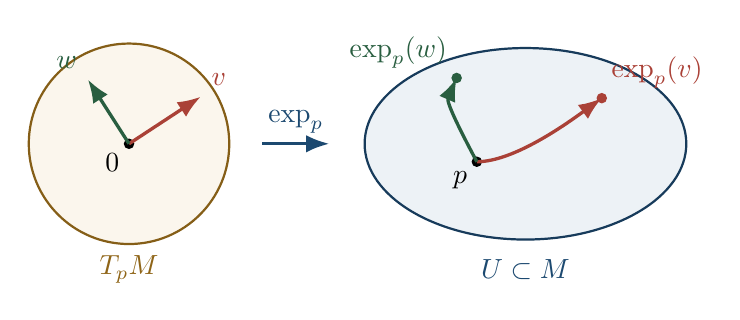
\begin{tikzpicture}[>=Latex,scale=.95]
  \fill[manifoldgold!8] (-3.3,0) circle (1.34);
  \draw[manifoldgold!65!black,thick] (-3.3,0) circle (1.34);
  \fill[manifoldblue!8] (2,0) ellipse (2.15 and 1.28);
  \draw[manifoldblue!65!black,thick] (2,0) ellipse (2.15 and 1.28);
  \coordinate (z) at (-3.3,0);
  \coordinate (pa) at (1.35,-.24);
  \fill[black] (z) circle (2pt) node[below left] {$0$};
  \fill[black] (pa) circle (2pt) node[below left] {$p$};
  \draw[manifoldred,very thick,->] (z)--(-2.34,.63) node[above right] {$v$};
  \draw[manifoldgreen!75!black,very thick,->] (z)--(-3.85,.86) node[above left] {$w$};
  \draw[manifoldred,very thick,->] (pa) .. controls (1.84,-.24) and (2.54,.26) .. (3.02,.61);
  \draw[manifoldgreen!75!black,very thick,->] (pa) .. controls (1.10,.23) and (.94,.56) .. (1.08,.88);
  \fill[manifoldred] (3.02,.61) circle (2pt) node[above right] {$\exp_p(v)$};
  \fill[manifoldgreen!75!black] (1.08,.88) circle (2pt) node[above left] {$\exp_p(w)$};
  \draw[manifoldblue!80!black,very thick,->] (-1.52,0)--(-.62,0)
       node[midway,above] {$\exp_p$};
  \node[manifoldgold!70!black] at (-3.3,-1.68) {$T_pM$};
  \node[manifoldblue!80!black] at (2,-1.68) {$U\subset M$};
\end{tikzpicture}
\caption{Wektory w $T_pM$ opisują krótkie geodezyjne wychodzące z $p$. Odwzorowanie $\exp_p$ zamienia małą kulę wektorów na otoczenie punktu.}
\label{fig:exp-normalne}
\end{figure}

Słowo „normalne” dotyczy tutaj współrzędnych,
nie wektora normalnego do powierzchni.
Równość $\Gamma(p)=0$ zachodzi w \emph{jednym}
punkcie. Nie daje podstaw do wyzerowania
wszystkich symboli na całej zakrzywionej
rozmaitości.

\section{Lemat Gaussa i lokalna minimalność}
\label{sec:gauss-geodezyjna-minimalna}

Współrzędne normalne pozwalają rozdzielić
ruch \emph{od} $p$ od ruchu \emph{w poprzek}.
Lemat Gaussa mówi, że te kierunki są
ortogonalne w metryce, a nie tylko na rysunku.

\begin{lemat}[Gaussa]
\label{lem:gaussa-exp}
Jeżeli $v$ leży w otwartej dziedzinie $D_p$ odwzorowania
$\exp_p$ i
$w\in T_pM$, to
\begin{equation}\label{eq:lemat-gaussa}
 g_{\exp_p(v)}\!\left(
   \dd(\exp_p)_v(v),\dd(\exp_p)_v(w)\right)
   =g_p(v,w).
\end{equation}
W szczególności pochodna w kierunku radialnym
jest prostopadła do obrazów kierunków
stycznych do sfery $|v|_g=\mathrm{const}$.
\end{lemat}
\begin{proof}
Rozpatrzmy dwuwymiarową rodzinę geodezyjnych
$F(s,t)=\exp_p(t(v+sw))$, $0\leq t\leq1$,
przy małym $s$. Połóżmy
$T=\partial_tF$, $V=\partial_sF$.
Każda krzywa $t\mapsto F(s,t)$ jest geodezyjną,
więc $D_tT=0$, a jej kwadrat prędkości
jest stały i równy $g_p(v+sw,v+sw)$.
Z braku torsji $D_tV=D_sT$. Zatem
\[
 \partial_t g(V,T)
 =g(D_sT,T)+g(V,D_tT)
 =\tfrac12\partial_s g(T,T).
\]
W $s=0$ prawa strona jest stałą $g_p(v,w)$.
Ponadto $V(0)=0$, gdyż $F(s,0)=p$.
Całkując po $t$ od $0$ do $1$, dostajemy
$g(V(1),T(1))=g_p(v,w)$.
Reguła łańcuchowa daje
$V(1)=\dd(\exp_p)_v(w)$ i
$T(1)=\dd(\exp_p)_v(v)$, czyli tezę.
\end{proof}

W normalnym otoczeniu zapiszmy niezerowe
$v=r\theta$, gdzie $r=|v|_g$ i
$|\theta|_g=1$. Lemat daje lokalnie postać
\begin{equation}\label{eq:metryka-biegunowo-normalna}
 g=\dd r^2+h_{ab}(r,\theta)
                 \dd\theta^a\dd\theta^b.
\end{equation}
Rzeczywiście $\partial_r=\dd\exp_{r\theta}(\theta)$
ma długość $1$ (stała prędkość radialnej
geodezyjnej), a kierunki kątowe są do niego
prostopadłe. Macierz $(h_{ab})$ jest dodatnio
określona dla $r>0$ w tym otoczeniu.

\begin{twierdzenie}[Krótka geodezyjna minimalizuje]
\label{thm:lokalna-minimalnosc-geodezyjnej}
Istnieje $\rho>0$ takie, że dla każdego
$q=\exp_p(v)$ z $|v|_g<\rho$ radialna
geodezyjna $\gamma(t)=\exp_p(tv)$,
$0\leq t\leq1$, spełnia
\begin{equation}\label{eq:odleglosc-exp-lokalna}
 d_g(p,q)=L_g(\gamma)=|v|_g.
\end{equation}
Dla $v\ne0$ każda odcinkami $C^1$ droga osiągająca tę
długość ma ten sam ślad radialny i przebiega go bez cofania;
może przy tym zatrzymywać się na pewnych odcinkach parametru.
Dla $v=0$ jedyną drogą o długości zero jest droga stała. W szczególności \emph{każdy}
dostatecznie krótki fragment dowolnej
geodezyjnej riemannowskiej minimalizuje
odległość między swoimi końcami.
\end{twierdzenie}
\begin{proof}
Wybierzmy $\rho$ tak małe, by
$\exp_p$ było dyfeomorfizmem na kuli $B_{3\rho}(0)$.
W szczególności domknięcie $\overline B_{2\rho}(0)$
leży w tej dziedzinie, a jego obraz jest zwarty. W normalnych współrzędnych
dowolną odcinkami $C^1$ krzywą $\alpha$
biegnącą od $p$ do $q$ i pozostającą
w obrazie tej kuli piszemy dla $r>0$
przez $r(t),\theta(t)$. Z \eqref{eq:metryka-biegunowo-normalna}
wynika
\[
 |\dot\alpha|_g^2
 =(\dot r)^2+h_{ab}\dot\theta^a\dot\theta^b
 \geq (\dot r)^2,
 \qquad
 L_g(\alpha)\geq\int|\dot r|\,\dd t
 \geq r(q)=|v|_g.
\]
W punkcie $p$ funkcja $r$ nie musi być gładka.
Jednak $u(t)=\exp_p^{-1}(\alpha(t))$ jest odcinkami $C^1$,
a $r(t)=|u(t)|_g$ jest lipschitzowska na zwartym przedziale,
więc absolutnie ciągła. Pochodna $\dot r$ istnieje prawie
wszędzie i jest równa zero prawie wszędzie na zbiorze
$\{t:r(t)=0\}$: w każdym wewnętrznym punkcie tego zbioru,
w którym pochodna istnieje, $r$ ma minimum. Nierówność
$|\dot\alpha|_g\geq|\dot r|$ zachodzi zatem prawie wszędzie,
co uzasadnia całkowanie również przy wielokrotnych powrotach do $p$. Radialna geodezyjna
ma $\dot\theta=0$, $\dot r\geq0$ i długość
$|v|_g$, więc osiąga dolne ograniczenie.
Równość w drugiej nierówności całkowej wymaga
$\dot r\geq0$ prawie wszędzie, czyli $r$ jest niemalejąca.
Zbiór $\{r>0\}$ jest wtedy jednym końcowym przedziałem.
Na nim równość w pierwszej nierówności i dodatnia
określoność $h$ dają $\dot\theta=0$ prawie wszędzie.
Na każdym zwartym podprzedziale $\theta$ jest odcinkami
$C^1$, a więc stała. To dowodzi jednoznaczności śladu;
chwile postoju odpowiadają stałym odcinkom funkcji $r$.

Jeśli $\alpha$ opuści obraz $B_{2\rho}(0)$,
jej pierwszy punkt wyjścia ma promień $2\rho$.
Poprzednia nierówność na początkowym kawałku
daje $L_g(\alpha)\geq2\rho>|v|_g$.
Porównaliśmy więc także drogi wychodzące
z otoczenia, co jest potrzebne dla odległości
$d_g$ zdefiniowanej przez \emph{wszystkie}
dopuszczalne krzywe. Dla dowolnej geodezyjnej
powtarzamy argument, biorąc za $p$ jej punkt
początkowy i skracając przedział parametru.
\end{proof}

Z dowodu wynika również identyfikacja małych kul. Dla
$0<a<\rho$ mamy
\begin{equation}\label{eq:male-kule-normalne}
 B^g_a(p)=\exp_p(B_a(0)),\qquad
 \overline B^g_a(p)=\exp_p(\overline B_a(0)).
\end{equation}
Tutaj $\overline B^g_a(p)=\{q:d_g(p,q)\leq a\}$.
Każdy punkt spoza $\exp_p(B_{2\rho}(0))$ ma odległość
co najmniej $2\rho$ od $p$, na mocy argumentu z pierwszym
wyjściem. Wewnątrz tego otoczenia ten sam rachunek
radialny daje $d_g(p,\exp_p(v))=|v|_g$.
Stąd obie równości i zwartość małych kul domkniętych
oraz sfer metrycznych, bez założenia zupełności $M$.

Pierwsza wariacja dowodziła, że krzywa minimalna
\emph{musi} być geodezyjną; lemat Gaussa dowiódł,
że krótka geodezyjna \emph{jest} krzywą minimalną.
Na długich odcinkach drugie zdanie może
przestać być prawdziwe. Druga wariacja i pola
Jacobiego w Sekcji~\ref{sec:druga-wariacja-jacobi}
opiszą, jak krzywizna wpływa na utratę tej własności.

\section{Geodezyjne w geometriach modelowych}
\label{sec:geodezyjne-modele}

\begin{przyklad}[Przestrzeń euklidesowa]
\label{prz:geodezyjne-euklidesowe}
Dla $g=\sum_i(\dd x^i)^2$ symbole Christoffela
znikają. Równanie $\ddot x=0$ ma rozwiązanie
$\gamma_{p,v}(t)=p+tv$, a $\exp_p(v)=p+v$
na całym $T_p\R^n$. Dla dowolnej krzywej
$\alpha:[a,b]\to\R^n$ od $p$ do $q$
nierówność trójkąta dla całki daje
\[
 L(\alpha)=\int_a^b|\dot\alpha|\,\dd t
 \geq\left|\int_a^b\dot\alpha\,\dd t\right|
 =|q-p|.
\]
Odcinek prosty osiąga tę wartość i jest
globalnie minimalny.
\end{przyklad}

\begin{figure}[htbp]
\centering
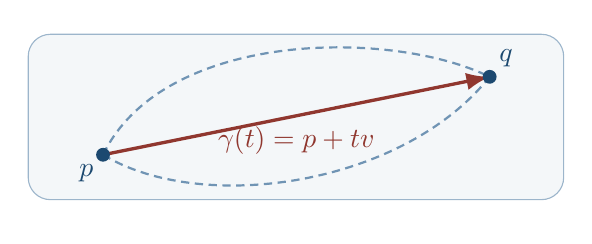
\begin{tikzpicture}[>=Latex,scale=1]
  \fill[manifoldblue!5,rounded corners=8pt]
     (-3.4,-1.05) rectangle (3.4,1.05);
  \draw[manifoldblue!45,rounded corners=8pt]
     (-3.4,-1.05) rectangle (3.4,1.05);
  \coordinate (p) at (-2.45,-.48);
  \coordinate (q) at (2.46,.51);
  \draw[manifoldred!85!black,very thick,->]
     (p)--(q) node[pos=.50,below] {$\gamma(t)=p+tv$};
  \draw[manifoldblue!65,thick,densely dashed]
     (p) .. controls (-1.68,1.11) and (1.22,1.12) .. (q);
  \draw[manifoldblue!65,thick,densely dashed]
     (p) .. controls (-1.2,-1.24) and (1.35,-.88) .. (q);
  \fill[manifoldblue!80!black] (p) circle (2.5pt)
     node[below left] {$p$};
  \fill[manifoldblue!80!black] (q) circle (2.5pt)
     node[above right] {$q$};
\end{tikzpicture}
\caption{Euklidesowa geodezyjna między $p$ i $q$ jest prostym odcinkiem. Przykładowe drogi przerywane mają większą długość.}
\label{fig:geodezyjna-euklidesowa}
\end{figure}

\begin{przyklad}[Sfera: wielkie koła i antypody]
\label{prz:geodezyjne-sfera}
Niech $R>0$, $p\in S_R^2\subset\R^3$ i $v\perp p$,
$s=|v|$. Dla $v\ne0$ geodezyjna i odwzorowanie
wykładnicze mają postać
\begin{equation}\label{eq:exp-sfera}
 \gamma_{p,v}(t)
 =\cos\!\left(\frac{st}{R}\right)p
  +\frac{R}{s}\sin\!\left(\frac{st}{R}\right)v,
 \qquad \exp_p(v)=\gamma_{p,v}(1).
\end{equation}
Dla $v=0$ rozumiemy granicę, czyli $\exp_p(0)=p$.
Różniczkując dwa razy, dostajemy
$\ddot\gamma=-(s^2/R^2)\gamma$.
Wektor $\gamma$ jest normalny do sfery,
więc jego rzut na przestrzeń styczną jest zerowy.
Ze Stwierdzenia~\ref{prop:koneksja-projekcja} wynika
$D\dot\gamma/\dd t=0$. Są to łuki wielkich kół.

Dla bieguna $p$ i $r=R\theta$ metryka
\eqref{eq:metryka-sfery} przyjmuje postać
\[
 g=\dd r^2+R^2\sin^2(r/R)\,\dd\phi^2,
 \qquad 0<r<\pi R.
\]
Jest to konkretny przypadek
\eqref{eq:metryka-biegunowo-normalna}.
Łuk od $p$ do punktu w odległości kątowej
$\theta<\pi$ ma długość $R\theta$ i jest
minimalny. Funkcja
$r(x)=R\arccos(\langle p,x\rangle/R^2)$
jest określona na całej sferze i gładka
poza biegunami $p,-p$. Lokalny wzór na metrykę
działa po zmianie kąta $\phi$ także przy
przekroczeniu szwu mapy; dla drogi omijającej
antypodę nadal $L\geq\int|\dot r|\geq R\theta$.
Dla drogi przechodzącej przez antypodę najpierw stosujemy
to oszacowanie do pierwszego osiągnięcia poziomu
$r=\pi R-\varepsilon$. Przejście $\varepsilon\downarrow0$
daje długość co najmniej $\pi R>R\theta$.
Przy przejściach przez $p$ argument absolutnej ciągłości
z dowodu Twierdzenia~\ref{thm:lokalna-minimalnosc-geodezyjnej}
uzasadnia całkowanie mimo niegładkości $r$.
Przy $r=\pi R$ wszystkie kierunki jednostkowe
trafiają do antypody $-p$: istnieje wiele
minimalnych półokręgów o długości $\pi R$.
Za antypodą przedłużony łuk nadal jest
geodezyjną, lecz nie minimalizuje długości.
Sfera pozostaje geodezyjnie zupełna: wzór
\eqref{eq:exp-sfera} działa dla każdego $t\in\R$.
\end{przyklad}

\begin{figure}[htbp]
\centering
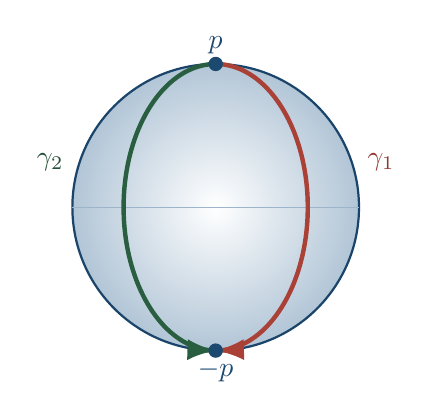
\begin{tikzpicture}[>=Latex,scale=1.04]
  % Rzut (X,Y,Z) -> (X,Z); oba półokręgi mają Y>=0.
  \shade[inner color=white,outer color=manifoldblue!35] (0,0) circle (1.75);
  \draw[manifoldblue!75!black,thick] (0,0) circle (1.75);
  \draw[manifoldblue!45] (-1.75,0)--(1.75,0);
  \draw[manifoldred,ultra thick,->]
    plot[domain=0:180,samples=80,variable=\u]
      ({1.75*sin(40)*sin(\u)},{1.75*cos(\u)});
  \draw[manifoldgreen!75!black,ultra thick,->]
    plot[domain=0:180,samples=80,variable=\u]
      ({-1.75*sin(40)*sin(\u)},{1.75*cos(\u)});
  \fill[manifoldblue!80!black] (0,1.75) circle (2.5pt) node[above] {$p$};
  \fill[manifoldblue!80!black] (0,-1.75) circle (2.5pt) node[below] {$-p$};
  \node[manifoldred!85!black] at (2.02,.55) {$\gamma_1$};
  \node[manifoldgreen!65!black] at (-2.02,.55) {$\gamma_2$};
\end{tikzpicture}
\caption{Dwa różne półokręgi wielkich kół łączą $p$ z antypodą.
Każdy ma długość $\pi R$. Rysunek jest rzutem ortogonalnym:
półokręgi widać jako połówki elips, a równik jako odcinek.
Przedłużenie łuku za antypodę nie minimalizuje już długości od $p$.}
\label{fig:geodezyjne-antypody}
\end{figure}

\begin{przyklad}[Przestrzeń hiperboliczna]
\label{prz:geodezyjne-hiperboliczne}
W modelu górnej półprzestrzeni z
\eqref{eq:hip-polprzestrzen} pionowa krzywa
\[
 \gamma(s)=(x_0,y_0e^s),\qquad s\in\R,
\]
ma prędkość hiperboliczną $1$.
W dwuwymiarowym przypadku wzory
\eqref{eq:gamma-hiperboliczna} dają
$\ddot y-(\dot y)^2/y=0$ i równanie
poziome jest spełnione, więc to geodezyjna.
Dla krzywej łączącej $(x_0,y_0)$ z
$(x_0,y_1)$ mamy
\[
 L=\int\frac{\sqrt{|\dot x|^2+\dot y^2}}{y}\,\dd t
 \geq\int\left|\frac{\dot y}{y}\right|\dd t
 \geq\left|\log\frac{y_1}{y_0}\right|.
\]
Pionowa geodezyjna osiąga tę wartość.
Zatem granica $y=0$ jest w nieskończonej
odległości wzdłuż pionu, choć na rysunku
euklidesowym wydaje się bliska.

To nie są wszystkie geodezyjne półprzestrzeni.
W wymiarze dwa równania geodezyjnej z
\eqref{eq:gamma-hiperboliczna} mają postać
\[
 \ddot x-\frac{2\dot x\dot y}{y}=0,
 \qquad
 \ddot y+\frac{\dot x^2-\dot y^2}{y}=0.
\]
Rozpatrzmy niestałą geodezyjną i parametryzujmy ją długością łuku:
$(\dot x^2+\dot y^2)/y^2=1$. Pierwsze równanie
po przekształceniu daje
$\frac{\dd}{\dd s}(\dot x/y^2)=0$.
Jeżeli stała $c=\dot x/y^2$ jest zerowa,
otrzymujemy pionową prostą. Jeśli $c\ne0$,
to $\dot x=cy^2$ oraz
$\dot y^2=y^2(1-c^2y^2)$. Eliminując parametr,
\[
 \frac{\dd x}{\dd y}
   =\pm\frac{cy}{\sqrt{1-c^2y^2}},
 \qquad
 (x-x_c)^2+y^2=c^{-2}
\]
po scałkowaniu na odcinkach monotoniczności $y$.
Jest to półokrąg o środku $(x_c,0)$,
przecinający brzeg $y=0$ prostopadle.
Punkt zwrotny wysokości nie jest końcem geodezyjnej.
Dla $R_0=1/|c|$ jawne rozwiązanie jednostkowe to
\[
 x(s)=x_c+\operatorname{sgn}(c)R_0\tanh(s-s_0),\qquad
 y(s)=\frac{R_0}{\cosh(s-s_0)},\qquad s\in\R.
\]
Podstawienie sprawdza oba równania i stałą $\dot x/y^2=c$;
rozwiązanie przechodzi gładko przez maksimum $y$ w $s=s_0$.
W wymiarze $n>2$ każda geodezyjna mieści się
w pewnej pionowej dwupłaszczyźnie: odbicie
w niej jest izometrią, zachowuje punkt i wektor
początkowy, a jednoznaczność rozwiązania
równania geodezyjnej wymusza niezmienniczość
krzywej. Tam stosujemy powyższy rachunek. W wymiarze $1$
model jest półprostą z metryką $\dd y^2/y^2$ i pozostają
wyłącznie geodezyjne pionowe oraz krzywe stałe.

W modelu hiperboloidy z
Przykładu~\ref{prz:trzy-modele-hiperboliczne}
piszemy $\langle(t,z),(t',z')\rangle_L
=-tt'+z\cdot z'$ i $\langle p,p\rangle_L=-1$.
Dla $v\in T_p\mathcal H^n$, $s=|v|_g$, mamy
\begin{equation}\label{eq:exp-hiperboloida}
 \exp_p(v)=\cosh(s)p+\frac{\sinh(s)}{s}v,
\end{equation}
z wartością graniczną $p$ przy $s=0$.
Dokładniej, dla jednostkowego $w\in T_p\mathcal H^n$
cała geodezyjna ma wzór
$\gamma_{p,w}(\tau)=\cosh\tau\,p+\sinh\tau\,w$.
Leży w przecięciu hiperboloidy z dwuwymiarową
płaszczyzną liniową $\operatorname{span}(p,w)$
przechodzącą przez początek przestrzeni Minkowskiego.
Rzeczywiście $\langle p,v\rangle_L=0$;
podstawienie daje normę lorentzowską $-1$,
a znak współrzędnej czasowej pozostaje dodatni przez ciągłość.
Rzutowanie pochodnej płaskiej działa tu także dla iloczynu
lorentzowskiego: przestrzeń styczna jest niezdegenerowana,
a jej dopełnieniem ortogonalnym jest prosta rozpięta przez
wektor położenia $x$, o $\langle x,x\rangle_L=-1$.
Ten sam dowód zgodności i braku torsji co w
Stwierdzeniu~\ref{prop:koneksja-projekcja} daje
\[
 \nabla_XY=D_XY+\langle D_XY,x\rangle_Lx
          =D_XY-g(X,Y)x.
\]
Dla $\gamma(t)=\cosh(st)p+\sinh(st)v/s$ mamy
$\ddot\gamma=s^2\gamma$ i $g(\dot\gamma,\dot\gamma)=s^2$,
więc rzeczywiście $D\dot\gamma/\dd t=0$.
Wzór działa dla każdego $t$, co dowodzi zupełności geodezyjnej.

Uzasadnijmy dziedzinę odwrotnej funkcji hiperbolicznej.
Jeśli $p=(\sqrt{1+|z|^2},z)$ i $q=(\sqrt{1+|w|^2},w)$,
to nierówność Cauchy'ego--Schwarza daje
\[
 -\langle p,q\rangle_L
 \geq\sqrt{1+|z|^2}\sqrt{1+|w|^2}-|z|\,|w|\geq1.
\]
Druga nierówność po podniesieniu do kwadratu sprowadza się
do $(|z|-|w|)^2\geq0$; równość w obu zachodzi dokładnie
dla $z=w$. Dla dowolnego $q\in\mathcal H^n$ połóżmy
$s=\operatorname{arcosh}(-\langle p,q\rangle_L)$.
Gdy $q\ne p$, wektor
$v=\frac{s}{\sinh s}(q-\cosh(s)p)$
jest styczny w $p$, ma normę $s$ i spełnia
$\exp_p(v)=q$. Zatem $\exp_p$ jest także
surjekcją na $\mathcal H^n$.
Późniejszy Wniosek~\ref{cor:hopf-rinow-minimalna}
zapewni istnienie globalnej geodezyjnej minimalnej.
Jeśli $q=\exp_p(v)$, iloczyn z $p$ daje
$-\langle p,q\rangle_L=\cosh|v|_g$;
jednoznaczność dodatniego $|v|_g$
i wyrażenia \eqref{eq:exp-hiperboloida} pokazuje,
że $\exp_p$ jest różnowartościowe. Dlatego
\begin{equation}\label{eq:odleglosc-hiperboloida}
 d_{\mathcal H}(p,q)
 =\operatorname{arcosh}(-\langle p,q\rangle_L).
\end{equation}

W \emph{modelu kuli Poincarégo} z
\eqref{eq:hip-kula} skorzystajmy z izometrii
$P:B^n\to\mathcal H^n$ zapisanej w
Przykładzie~\ref{prz:trzy-modele-hiperboliczne}.
Ponieważ $P(0)=(1,0)$ i
$P^{-1}(t,z)=z/(t+1)$, obraz geodezyjnej
$\tau\mapsto(\cosh\tau,\sinh\tau\,e)$,
$|e|=1$, jest równy
\begin{equation}\label{eq:geodezyjna-dysk-radialna}
 \gamma_e(\tau)=\tanh(\tau/2)e.
\end{equation}
Wszystkie średnice dysku są więc geodezyjnymi
\emph{jako zbiory punktów}; parametr euklidesowy
na średnicy nie jest parametrem długości hiperbolicznej.

Pozostałe geodezyjne w dwuwymiarowym dysku są
łukami okręgów prostopadłych do brzegu $|u|=1$.
Oto rachunek wyjaśniający ten obraz. Geodezyjna
hiperboloidy leży w płaszczyźnie liniowej, którą
w $\R^{1,2}$ można zapisać jako
$\alpha t+b\cdot z=0$. Po podstawieniu
$P(u)=((1+|u|^2)/(1-|u|^2),2u/(1-|u|^2))$
jej obraz odwrotny spełnia
\[
 \alpha(1+|u|^2)+2b\cdot u=0.
\]
Jeśli $\alpha=0$, to średnica $b\cdot u=0$.
Jeśli $\alpha\ne0$, po oznaczeniu $c=-b/\alpha$
dostajemy
\begin{equation}\label{eq:geodezyjna-dysk-okrag}
 |u-c|^2=|c|^2-1.
\end{equation}
Środek $c$ leży poza dyskiem: płaszczyzna geodezyjnej
przecina hiperboloidę, więc równanie ma rozwiązanie
$0<|u|<1$; stąd
$|b|\geq |\alpha|(1+|u|^2)/(2|u|)>|\alpha|$.
Kwadrat promienia
okręgu wynosi $|c|^2-1$. Warunek ten oznacza
prostopadłe przecięcie z okręgiem jednostkowym:
w punkcie przecięcia $u$ równanie okręgu daje
$u\cdot(u-c)=0$, więc promienie obu okręgów
są prostopadłe. W wymiarze $n>2$ geodezyjna
leży w odpowiednim dwuwymiarowym przekroju
kuli i ten sam opis działa w tym przekroju.

Izometria $F:B^n\to\mathbb H^n$ z
Przykładu~\ref{prz:trzy-modele-hiperboliczne}
przenosi opis dyskowy na pionowe proste
i półokręgi w półprzestrzeni. Izometrie
zachowują pochodną kowariantną, więc obrazy
geodezyjnych są geodezyjnymi. Zachowują też
długości, skąd z~\eqref{eq:odleglosc-hiperboloida}
otrzymujemy użyteczne wzory odległości:
\begin{align}\label{eq:odleglosci-modele-hiperboliczne}
 \cosh d_B(u,v)
  &=1+\frac{2|u-v|^2}
      {(1-|u|^2)(1-|v|^2)},\\
 \cosh d_{\mathbb H}((x,y),(x',y'))
  &=1+\frac{|x-x'|^2+(y-y')^2}{2yy'}.\notag
\end{align}
Pierwszy wzór pochodzi z wstawienia $P(u),P(v)$
do iloczynu Minkowskiego; drugi z podstawienia
$F^{-1}(x,y),F^{-1}(x',y')$ do pierwszego.
W szczególności
$d_B(0,u)=2\operatorname{artanh}|u|	o\infty$
przy $|u|\uparrow1$: widoczny brzeg dysku,
podobnie jak prosta $y=0$, nie leży w przestrzeni
hiperbolicznej.
\end{przyklad}

\begin{figure}[H]
\centering
\begin{tikzpicture}[>=Latex,scale=.91]
  \fill[manifoldblue!5] (-3.5,0) rectangle (3.5,2.65);
  \draw[manifoldblue!70!black,very thick] (-3.5,0)--(3.5,0)
       node[right] {$y=0$};
  \draw[manifoldblue!45!black,->] (-3.25,0)--(-3.25,2.55)
       node[above] {$y$};
  \draw[manifoldred,very thick,->] (-1.60,.30)--(-1.60,2.23);
  \fill[manifoldred] (-1.60,.55) circle (2.5pt)
       node[left] {$(x_0,y_0)$};
  \fill[manifoldred] (-1.60,1.85) circle (2.5pt)
       node[left] {$(x_0,y_1)$};
  \draw[manifoldgreen!75!black,very thick,->]
       ({1.1+1.7*cos(170)},{1.7*sin(170)})
       arc[start angle=170,end angle=19,radius=1.7];
  \draw[manifoldgold!70!black,densely dashed]
       (-.6,0) arc[start angle=180,end angle=0,radius=1.7];
  \node[manifoldgreen!60!black] at (1.28,2.38)
       {półokrąg prostopadły do brzegu};
  \node[manifoldblue!70!black] at (1.55,-.47)
       {brzeg w nieskończonej odległości};
\end{tikzpicture}
\caption{Geodezyjne w modelu górnej półpłaszczyzny: pionowa półprosta i półokrąg przecinający brzeg $y=0$ pod kątem prostym. Brzeg nie należy do przestrzeni hiperbolicznej.}
\label{fig:geodezyjne-hiperboliczne}
\end{figure}

\begin{figure}[H]
\centering
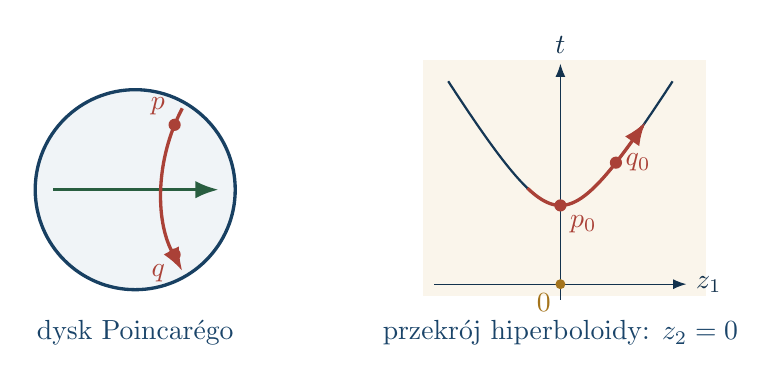
\begin{tikzpicture}[>=Latex,scale=1]
  \begin{scope}[shift={(-2.75,0)}]
    \fill[manifoldblue!7] (0,0) circle (1.27);
    \draw[manifoldblue!70!black,very thick] (0,0) circle (1.27);
    \draw[manifoldgreen!75!black,very thick,->]
       (-1.04,0)--(1.06,0);
    \draw[manifoldred,very thick,->]
       ({2*1.27+sqrt(3)*1.27*cos(152)},
        {sqrt(3)*1.27*sin(152)})
       arc[start angle=152,end angle=208,
           radius={sqrt(3)*1.27}];
    \fill[manifoldred] ({2*1.27+sqrt(3)*1.27*cos(158)},
        {sqrt(3)*1.27*sin(158)}) circle (2.2pt)
        node[above left] {$p$};
    \fill[manifoldred] ({2*1.27+sqrt(3)*1.27*cos(202)},
        {sqrt(3)*1.27*sin(202)}) circle (2.2pt)
        node[below left] {$q$};
    \node[manifoldblue!75!black] at (0,-1.82)
       {dysk Poincarégo};
  \end{scope}
  \begin{scope}[shift={(2.65,0)}]
    % Dokładny przekrój z_2=0: t=cosh(u), z_1=sinh(u).
    % Rysunek ma skalę poziomą 0.6 oraz przesunięcie pionowe -1.2.
    \fill[manifoldgold!9] (-1.75,-1.35) rectangle (1.85,1.65);
    \draw[manifoldblue!55!black,->] (-1.6,-1.2)--(1.6,-1.2)
      node[right] {$z_1$};
    \draw[manifoldblue!55!black,->] (0,-1.4)--(0,1.60)
      node[above] {$t$};
    \draw[manifoldblue!60!black,thick]
      plot[domain=-1.6:1.6,samples=90,variable=\u]
        ({.6*sinh(\u)},{cosh(\u)-1.2});
    \draw[manifoldred,very thick,->]
      plot[domain=-.65:1.35,samples=65,variable=\u]
        ({.6*sinh(\u)},{cosh(\u)-1.2});
    \fill[manifoldred] (0,-.2) circle (2.2pt)
      node[below right] {$p_0$};
    \fill[manifoldred] ({.6*sinh(1)},{cosh(1)-1.2}) circle (2.2pt)
      node[right] {$q_0$};
    \fill[manifoldgold!80!black] (0,-1.2) circle (1.8pt)
      node[below left] {$0$};
    \node[manifoldblue!75!black] at (0,-1.82)
      {przekrój hiperboloidy: $z_2=0$};
  \end{scope}
\end{tikzpicture}
\caption{Po lewej geodezyjne dysku: średnica i łuk okręgu
prostopadłego do brzegu (końce na brzegu nie należą do geodezyjnej).
Po prawej dokładny przekrój hiperboloidy $t^2-z_1^2-z_2^2=1$,
$t>0$, płaszczyzną liniową $z_2=0$. Czerwona geodezyjna ma
postać $(\cosh u,\sinh u,0)$; zaznaczono $p_0$ dla $u=0$
i $q_0$ dla $u=1$. Płaszczyzna przekroju zawiera początek $0$.}
\label{fig:geodezyjne-dysk-hiperboloida}
\end{figure}

\section{Twierdzenie Hopfa--Rinowa}
\label{sec:hopf-rinow}

W lokalnym twierdzeniu minimalnym odcinek był
krótki. Żeby mieć geodezyjną minimalną między \emph{dowolnymi}
punktami, potrzebujemy warunku, który zabrania
geodezyjnej uciec z rozmaitości w skończonym
czasie. Dla spójnej rozmaitości riemannowskiej
równoważne są dwa pozornie różne rodzaje
zupełności.

\begin{definicja}[Dwa znaczenia zupełności]
\index{dwa znaczenia zupelnosci@Dwa znaczenia zupełności}
\label{def:zupelnosc-geodezyjna}
$(M,g)$ jest \emph{metrycznie zupełna}, gdy
każdy ciąg Cauchy'ego dla $d_g$ ma granicę w $M$.
Jest \emph{geodezyjnie zupełna}, gdy każdą
geodezyjną można przedłużyć do parametru
z całej $\R$.
\end{definicja}

Do dowodu potrzebne jest spostrzeżenie o narożniku.
Jeżeli dwie jednostkowe geodezyjne składają się w drogę
minimalną, ich wektory styczne w punkcie sklejenia $x$
muszą być równe. Oznaczmy je przez $T_-,T_+$,
a chwilę sklejenia przez $t_0$.
W mapie wokół $x$ wybieramy ciągłe, kawałkami gładkie
pole wariacyjne o małym nośniku wokół chwili sklejenia,
takie że $V(t_0)=T_+-T_-$. Mnożenie jego współrzędnych
przez funkcję odcinającą realizuje taką wariację przez
dodanie $sV$ we współrzędnych, przy nieruchomych końcach.
Dla małego $s$ oba kawałki pozostają regularne.
Wzór pierwszej wariacji na obu geodezyjnych ma zerowe
składniki całkowe, a wyraz narożnikowy wynosi
\[
 g(T_+-T_-,T_--T_+)=-|T_+-T_-|_g^2.
\]
Jeśli styczne są różne, długość maleje dla małego $s>0$,
co przeczy minimalności. Przy jednakowych niezerowych
prędkościach ten argument stosujemy po wspólnym skalowaniu.

\begin{lemat}[Jeden punkt z pełnym odwzorowaniem wykładniczym]
\label{lem:exp-p-minimalna-kazdy-punkt}
Niech $M$ będzie spójną rozmaitością riemannowską bez brzegu.
Jeżeli dla pewnego $p\in M$ odwzorowanie $\exp_p$ jest określone na całym $T_pM$,
to każdy $q\in M$ można połączyć z $p$
geodezyjną o długości $d_g(p,q)$.
\end{lemat}
\begin{proof}
Jeśli $q=p$, bierzemy stałą geodezyjną.
Niech $r=d_g(p,q)>0$. Wybierzmy małą
kulę $B^g_\varepsilon(p)$ spełniającą
\eqref{eq:male-kule-normalne} i
$0<\delta<\min(\varepsilon,r)$.
Sfera $S_\delta(p)=\exp_p\{v:|v|=\delta\}$
jest zwarta jako obraz zwykłej zwartej sfery.
Funkcja $z\mapsto d_g(z,q)$ jest ciągła,
więc osiąga na niej minimum w punkcie $m$.
Każda droga z $p$ do $q$ przecina tę sferę.
Jej część do pierwszego przecięcia ma długość
co najmniej $\delta$, pozostała zaś co najmniej
$d_g(z,q)\geq d_g(m,q)$. Z drugiej strony
nierówność trójkąta daje
\begin{equation}\label{eq:hopf-pierwsza-sfera}
 r=\delta+d_g(m,q).
\end{equation}
Niech $\gamma:[0,\infty)\to M$ będzie
jednostkową geodezyjną od $p$ przez $m$.
Istnieje dla wszystkich $t\geq0$: dla danego
$t$ punkt $\gamma(t)=\exp_p(t\dot\gamma(0))$
jest określony, a jednoznaczność skleja te odcinki.
Rozważmy zamknięty zbiór
\[
 A=\{t\in[0,r]:t+d_g(\gamma(t),q)=r\}.
\]
Z \eqref{eq:hopf-pierwsza-sfera} wiemy, że
$\delta\in A$. Jeśli największy punkt
$t_*$ zbioru $A$ byłby mniejszy od $r$,
połóżmy $x=\gamma(t_*)$ i wybierzmy małą
normalną sferę $S_\eta(x)$ o promieniu
$0<\eta<d_g(x,q)$, tak by $\eta$ mieściło się
również w normalnym otoczeniu $x$.
Niech $m'$ minimalizuje $z\mapsto d_g(z,q)$
na $S_\eta(x)$. To samo rozumowanie
z pierwszym wyjściem z kuli daje
\begin{equation}\label{eq:hopf-druga-sfera}
 d_g(x,q)=\eta+d_g(m',q),\qquad
 r=t_*+\eta+d_g(m',q).
\end{equation}

Nierówność trójkąta i droga przez $x,m'$ dają
\[
 r\leq d_g(p,m')+d_g(m',q)
   \leq t_*+\eta+d_g(m',q)=r.
\]
Zachodzi więc równość: sklejenie $\gamma|_{[0,t_*]}$
z krótką radialną geodezyjną z $x$ do $m'$
minimalizuje długość od $p$ do $m'$.
Obie części są jednostkowe, zatem spostrzeżenie
o narożniku wymusza zgodność ich stycznych w $x$.
Jednoznaczność równania geodezyjnej daje
$m'=\gamma(t_*+\eta)$. Wtedy
\eqref{eq:hopf-druga-sfera} mówi, że
$t_*+\eta\in A$, sprzeczność z maksymalnością
$t_*$. Musi więc być $r\in A$,
czyli $d_g(\gamma(r),q)=0$ i $\gamma(r)=q$.
Ponieważ $\gamma$ ma prędkość $1$,
jej długość na $[0,r]$ wynosi $r=d_g(p,q)$.
\end{proof}

\begin{twierdzenie}[Hopfa--Rinowa]
\label{thm:hopf-rinow-geodezyjne}
Niech $(M,g)$ będzie niepustą, spójną rozmaitością
riemannowską bez brzegu. Równoważne są warunki:
\begin{enumerate}[label=(\roman*)]
\item $(M,d_g)$ jest zupełną przestrzenią metryczną;
\item każda maksymalna geodezyjna jest określona
      na całej $\R$;
\item dla pewnego $p\in M$ mamy $D_p=T_pM$,
      czyli $\exp_p$ jest określone wszędzie;
\item każdy domknięty i ograniczony w metryce
      $d_g$ podzbiór $M$ jest zwarty.
\end{enumerate}
Gdy warunki zachodzą, w (iii) można napisać
\emph{dla każdego} $p\in M$.
\end{twierdzenie}
\begin{proof}
Pokażemy kolejno (i)$\Rightarrow$(ii)
$\Rightarrow$(iii)$\Rightarrow$(iv)$\Rightarrow$(i).

\emph{(i)$\Rightarrow$(ii).}
Jeśli jednostkowa geodezyjna
$\gamma:[0,b)\to M$ miałaby maksymalny
skończony prawy koniec $b$, to
$d_g(\gamma(s),\gamma(t))\leq|s-t|$.
Dla dowolnego ciągu $t_j\uparrow b$ ciąg $\gamma(t_j)$
jest Cauchy'ego, więc zbiega do pewnego $z\in M$.
Oszacowanie odległości przez $|s-t|$ daje wtedy
$\gamma(t)\to z$ dla wszystkich $t\uparrow b$.
W mapie wokół $z$ macierz $G$ jest dodatnio
określona i na mniejszym zwartym otoczeniu
jednostajnie porównywalna z macierzą
euklidesową. Stałość prędkości geodezyjnej
ogranicza więc jej współczynniki $\dot x^i$.
Symbole $\Gamma^k_{ij}$ są tam ograniczone;
równanie~\eqref{eq:geodezyjna-ode} ogranicza
również $\ddot x^k$. Stąd $x(t)$ i $\dot x(t)$
mają granice przy $t\uparrow b$.
Lokalne twierdzenie ODE, uruchomione od tych
danych w chwili $b$, przedłuża geodezyjną
za $b$ -- sprzeczność. Analogicznie na lewym
końcu. Dla dowolnej stałej prędkości
przeskalowujemy parametr; geodezyjne o zerowej prędkości
są stałe i istnieją przez cały czas.

\emph{(ii)$\Rightarrow$(iii).}
Każda $\gamma_{p,v}$ istnieje w chwili $1$,
więc $D_p=T_pM$ dla każdego $p$.

\emph{(iii)$\Rightarrow$(iv).}
Lemat~\ref{lem:exp-p-minimalna-kazdy-punkt}
daje dla każdego $q$ geodezyjną od $p$
o długości $d_g(p,q)$. Jeśli $C$ jest domknięte
i ograniczone, wybierzmy $R$ z
$d_g(p,q)\leq R$ dla wszystkich $q\in C$.
Każdy $q\in C$ ma postać $\exp_p(v_q)$
z $|v_q|\leq R$. Zatem
$C\subset\exp_p(\overline B_R(0))$.
Domknięta kula w skończenie wymiarowej
przestrzeni $T_pM$ jest zwarta, jej obraz
też jest zwarty, a domknięty podzbiór
tego obrazu jest zwarty. To dowodzi (iv).

\emph{(iv)$\Rightarrow$(i).}
Ciąg Cauchy'ego jest ograniczony;
domknięcie zbioru jego wyrazów jest
domknięte i ograniczone, więc zwarte.
Istnieje zbieżny podciąg, a własność Cauchy'ego
zmusza cały ciąg do tej samej granicy.
\end{proof}

\begin{wniosek}[Globalna geodezyjna minimalna]
\label{cor:hopf-rinow-minimalna}
Jeżeli $(M,g)$ jest spójna i zupełna, to
dowolne $p,q\in M$ łączy geodezyjna
o długości $d_g(p,q)$. W szczególności
każda zwarta rozmaitość riemannowska
jest geodezyjnie zupełna.
\end{wniosek}
\begin{proof}
Pierwszą tezę daje (ii)$\Rightarrow$(iii)
oraz Lemat~\ref{lem:exp-p-minimalna-kazdy-punkt}.
Dla zwartej $M$ argument stosujemy w każdej składowej
spójnej, która jest domknięta i zwarta. Każdy ciąg w niej
ma zbieżny podciąg; ciąg Cauchy'ego zbiega
do granicy tego podciągu. Zatem (i) zachodzi
i stosujemy Twierdzenie~\ref{thm:hopf-rinow-geodezyjne}.
\end{proof}

\begin{przyklad}[Dlaczego potrzebujemy zupełności]
W $M=\R^2\setminus\{0\}$ z metryką euklidesową
geodezyjna $\gamma(t)=(1-t,0)$ dociera do
usuniętego punktu w skończonym czasie $t=1$.
Nie można jej przedłużyć jako krzywej w $M$.
Punkty $(1/n,0)$ tworzą ciąg Cauchy'ego bez
granicy w $M$. Między $(-1,0)$ i $(1,0)$
infimum długości wynosi $2$, ale żadna krzywa
w $M$ go nie osiąga. Dolne ograniczenie $2$ daje
nierówność euklidesowa. Dwa odcinki osi, od $-1$ do
$-\varepsilon$ i od $\varepsilon$ do $1$, połączone
półokręgiem promienia $\varepsilon$, mają łączną długość
$2-2\varepsilon+\pi\varepsilon\to2$.
Równość w nierówności euklidesowej wymagałaby przebiegania
odcinka od $(-1,0)$ do $(1,0)$ bez cofania, a taki odcinek
przechodzi przez usunięty punkt.
\end{przyklad}

\begin{figure}[htbp]
\centering
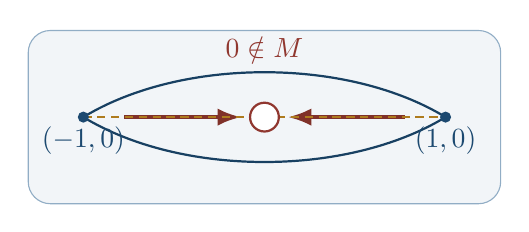
\begin{tikzpicture}[>=Latex,scale=1]
  \fill[manifoldblue!6,rounded corners=8pt]
       (-3,-1.10) rectangle (3,1.10);
  \draw[manifoldblue!50,rounded corners=8pt]
       (-3,-1.10) rectangle (3,1.10);
  \coordinate (a) at (-2.3,0);
  \coordinate (b) at (2.3,0);
  \draw[manifoldred!75!black,very thick,->] (1.78,0)--(.30,0);
  \draw[manifoldred!75!black,very thick,->] (-1.78,0)--(-.30,0);
  \draw[manifoldgold!85!black,thick,densely dashed] (a)--(b);
  \draw[manifoldblue!70!black,thick]
       (a) .. controls (-1.05,.76) and (1.05,.76) .. (b);
  \draw[manifoldblue!70!black,thick]
       (a) .. controls (-1.05,-.76) and (1.05,-.76) .. (b);
  \fill[white] (0,0) circle (5.2pt);
  \draw[manifoldred!85!black,thick] (0,0) circle (5.2pt);
  \node[manifoldred!85!black] at (0,.88) {$0\notin M$};
  \fill[manifoldblue!80!black] (a) circle (2pt) node[below] {$(-1,0)$};
  \fill[manifoldblue!80!black] (b) circle (2pt) node[below] {$(1,0)$};
\end{tikzpicture}
\caption{Na przebitej płaszczyźnie prosta geodezyjna może dotrzeć do usuniętego punktu w skończonym czasie. Drogi łączące punkty po przeciwnych stronach otworu omijają go; ich długości mogą zbliżać się do $2$, lecz żadna nie osiąga tej wartości.}
\label{fig:geodezyjna-przebita-plaszczyzna}
\end{figure}

\section{Miejsce cięcia i promień injektywności}
\label{sec:geodezyjne-miejsce-ciecia}

Krótki łuk geodezyjnej minimalizuje długość, ale
na sferze przestaje to robić po przejściu przez antypodę.
Na płaskim torusie ten sam kłopot pojawia się bez krzywizny:
różne proste w nakryciu mogą dojść do tego samego punktu.
Ustalimy dokładną granicę minimalności w każdym kierunku.
W tej sekcji $(M,g)$ jest spójną, zupełną rozmaitością
riemannowską bez brzegu, więc z Twierdzenia~\ref{thm:hopf-rinow-geodezyjne}
odwzorowanie $\exp_p$ jest określone na całym $T_pM$.

\begin{definicja}[Czas i miejsce cięcia]
\index{miejsce ciecia geodezyjnej@Miejsce cięcia geodezyjnej}
\index{zbior ciecia@Zbiór cięcia}
\label{def:czas-miejsce-ciecia}
Niech $p\in M$ i $u\in T_pM$ będzie jednostkowy.
Dla $\gamma_u(t)=\exp_p(tu)$ określamy \emph{czas cięcia}
\begin{equation}\label{eq:czas-ciecia}
 c_p(u)=\sup\{t\geq0:\ d_g(p,\gamma_u(t))=t\}
       \in(0,\infty].
\end{equation}
Jeżeli $c_p(u)<\infty$, punkt
$\gamma_u(c_p(u))$ jest \emph{miejscem cięcia geodezyjnej}
w kierunku $u$. \emph{Zbiór cięcia} punktu $p$ to
\[
 \operatorname{Cut}(p)
 =\{\exp_p(c_p(u)u):\ |u|_g=1,\ c_p(u)<\infty\}.
\]
Gdy wszystkie czasy cięcia są nieskończone, zbiór ten
jest pusty. Czas zależy od wybranego kierunku, a jeden
punkt zbioru może mieć kilka kierunków dochodzących.
\end{definicja}

Definicja mówi o \emph{odległości od $p$}, nie tylko
o tym, czy krzywa spełnia równanie geodezyjnej.
Jeśli odcinek $\gamma_u|_{[0,t]}$ jest minimalny,
to każdy jego początkowy pododcinek też jest minimalny:
krótsza droga do punktu pośredniego, połączona z resztą
odcinka, skróciłaby całość. Funkcja
$t\mapsto d_g(p,\gamma_u(t))-t$ jest ciągła.
Zbiór czasów z~\eqref{eq:czas-ciecia} jest zatem
przedziałem $[0,c_p(u)]$ przy skończonym $c_p(u)$,
a przy $c_p(u)=\infty$ jest całym $[0,\infty)$.
W szczególności skończony punkt cięcia \emph{jeszcze}
łączy z $p$ minimalny odcinek; każdy dłuższy fragment
tej samej geodezyjnej już nie minimalizuje.
Lokalna minimalność z~\eqref{eq:male-kule-normalne}
daje $c_p(u)>0$ dla wszystkich $u$ oraz wspólne
dodatnie dolne ograniczenie przy ustalonym $p$.

\begin{definicja}[Promień injektywności]
\index{promien injektywnosci@Promień injektywności}
\label{def:promien-injektywnosci}
\emph{Promieniem injektywności w punkcie $p$} nazywamy
\[
 \operatorname{inj}(p)=
 \sup\{r>0:\ \exp_p|_{B_r(0)}
       \text{ jest dyfeomorfizmem na swój obraz}\}.
\]
Tu $B_r(0)\subset T_pM$ jest otwartą kulą dla $g_p$;
dopuszczamy wartość $\infty$. Promień całej rozmaitości
to $\operatorname{inj}(M)=\inf_{p\in M}\operatorname{inj}(p)$.
Lokalne współrzędne normalne zapewniają
$\operatorname{inj}(p)>0$.
\end{definicja}

\begin{twierdzenie}[Cięcie wyznacza promień injektywności]
\label{thm:ciecie-promien-injektywnosci}
Dla spójnej, zupełnej rozmaitości riemannowskiej bez brzegu
i każdego $p\in M$ zachodzi
\begin{equation}\label{eq:inj-inf-ciecie}
 \operatorname{inj}(p)
 =\inf_{|u|_g=1}c_p(u)
 =d_g\bigl(p,\operatorname{Cut}(p)\bigr),
\end{equation}
 gdzie $d_g(p,\varnothing)=\infty$ oraz
 $\inf\varnothing=\infty$ dla rozmaitości wymiaru zero.
Jeżeli $0<r<\operatorname{inj}(p)$, to każdy
$v\in B_r(0)$ wyznacza jedyną minimalną geodezyjną
od $p$ do $\exp_p(v)$, a jej długość wynosi $|v|_g$.
\end{twierdzenie}
\begin{proof}
Oznaczmy $C=\inf_{|u|=1}c_p(u)$.
Najpierw wybierzmy $0<r<C$.
Dla $v=tu\in B_r(0)$, $t>0$, mamy $t<c_p(u)$,
więc $\gamma_u|_{[0,t]}$ minimalizuje. Co więcej,
można wybrać $\ell$ z $t<\ell<c_p(u)$
(gdy $c_p(u)=\infty$, dowolne $\ell>t$).
Odcinek do $\ell$ również minimalizuje.
Twierdzenie~\ref{thm:minimalna-bez-sprzezonego-wewnatrz}
z następnego rozdziału mówi, z pełnym dowodem przez
drugą wariację, że w jego wnętrzu nie ma punktu
sprzężonego z $p$. Na mocy
Stwierdzenia~\ref{prop:jacobi-dexp} różniczka
$\dd(\exp_p)_v$ jest więc odwracalna.
Przy $v=0$ wynika to z dowodu
Twierdzenia~\ref{thm:wspolrzedne-normalne}.

Pokażmy także injektywność $\exp_p$ na $B_r(0)$.
Jeśli $\exp_p(v)=\exp_p(w)=q$, to oba promienie
są minimalne, więc $|v|=|w|=d_g(p,q)=t$.
Dla $t=0$ mamy $v=w=0$. Dla $t>0$ załóżmy,
że $v\ne w$. Przedłużmy promień w kierunku $v/t$
do wybranego $\ell>t$ z $\ell<c_p(v/t)$.
Droga złożona z minimalnego promienia w kierunku $w/t$
do $q$ i dalszej części promienia w kierunku $v/t$
ma długość $\ell=d_g(p,\exp_p(\ell v/t))$.
Jest zatem minimalna, lecz w $q$ ma narożnik:
gdyby styczne się zgadzały, jednoznaczność równania
geodezyjnej dałaby $v=w$. Argument pierwszej wariacji
o narożniku przed Lematem~\ref{lem:exp-p-minimalna-kazdy-punkt}
wyklucza taki narożnik. Zatem $\exp_p$ jest injektywne.
Jako lokalny dyfeomorfizm i odwzorowanie injektywne
jest dyfeomorfizmem na swój obraz. Otrzymaliśmy
$\operatorname{inj}(p)\geq C$.

W drugą stronę załóżmy, że $r>C$.
Z definicji infimum istnieje kierunek jednostkowy
$u$ z $c_p(u)<r$; wybierzmy
$c_p(u)<t<r$ i połóżmy $q=\exp_p(tu)$.
Po czasie cięcia ten promień nie minimalizuje,
więc $d_g(p,q)<t$. Wniosek~\ref{cor:hopf-rinow-minimalna}
daje inną geodezyjną minimalną do $q$,
z wektorem początkowym $w$ o normie
$|w|=d_g(p,q)<t$. Oba różne wektory
$w,tu\in B_r(0)$ mają ten sam obraz przez $\exp_p$.
Na $B_r(0)$ nie może więc być ona injektywna,
tym bardziej nie jest dyfeomorfizmem.
To dowodzi $\operatorname{inj}(p)\leq C$.

Jeśli $c_p(u)<\infty$, ciągłość odległości daje
$d_g(p,\exp_p(c_p(u)u))=c_p(u)$.
Odległość od $p$ do zbioru cięcia jest zatem
infimum wszystkich skończonych $c_p(u)$.
Gdy takich nie ma, oba infima w~\eqref{eq:inj-inf-ciecie}
są równe $\infty$. Dowiedliśmy równości.
Unikalność minimalnej geodezyjnej dla $|v|<r$
wynika z już dowiedzionej injektywności:
każda minimalna geodezyjna od $p$ do $\exp_p(v)$
ma wektor początkowy tej samej długości $|v|<r$.
\end{proof}

W dowodzie potrzebowaliśmy informacji o punktach
sprzężonych, a więc o drugiej wariacji; jej pełne
wyprowadzenie jest w Sekcji~\ref{sec:druga-wariacja-jacobi}.
To, że cięcie może wynikać z dwóch różnych mechanizmów,
pokazuje następujący wniosek.

\begin{wniosek}[Co może się zdarzyć w miejscu cięcia]
\label{cor:ciecie-sprzezenie-lub-dwa-promienie}
Jeśli $c_p(u)<\infty$ i $q=\exp_p(c_p(u)u)$,
to albo istnieją co najmniej dwie różne minimalne
geodezyjne od $p$ do $q$, albo różniczka
$\dd(\exp_p)_{c_p(u)u}$ jest osobliwa.
Drugi przypadek oznacza sprzężenie wzdłuż wybranego
promienia zgodnie ze Stwierdzeniem~\ref{prop:jacobi-dexp}.
\end{wniosek}
\begin{proof}
Połóżmy $c=c_p(u)$ i $q_j=\exp_p((c+1/j)u)$.
Z Wniosku~\ref{cor:hopf-rinow-minimalna} wybierzmy
minimalne geodezyjne od $p$ do $q_j$ o wektorach
początkowych $w_j$. Ponieważ
$|w_j|=d_g(p,q_j)\leq c+1/j$, po przejściu do
podciągu $w_j\to w$. Ciągłość $\exp_p$ i odległości
daje $\exp_p(w)=q$ i $|w|=c$.
Jeśli $w\ne cu$, mamy dwa różne minimalne promienie
do $q$. Jeśli $w=cu$, a różniczka
$\dd(\exp_p)_{cu}$ byłaby odwracalna, twierdzenie
o funkcji odwrotnej dawałoby injektywność $\exp_p$
na otoczeniu $cu$. Dla dużych $j$ należałyby
do niego zarówno $w_j$, jak i $(c+1/j)u$,
chociaż ich obrazy są równe. To niemożliwe,
bo $|w_j|=d_g(p,q_j)<c+1/j$
na mocy definicji czasu cięcia.
\end{proof}

\begin{przyklad}[Okrągła sfera]
\label{prz:ciecie-sfera}
Na $S_R^2$ wzór~\eqref{eq:exp-sfera} daje dla jednostkowego
$u\in T_pS_R^2$ punkt
$\gamma_u(t)=\cos(t/R)p+R\sin(t/R)u$.
Przykład~\ref{prz:geodezyjne-sfera} wykazał,
że łuk jest minimalny dla $0\leq t\leq\pi R$.
Dla $\pi R<t<2\pi R$ drugi łuk tego samego
wielkiego koła, biegnący przeciwnie, ma długość
$2\pi R-t<t$. Stąd $c_p(u)=\pi R$ dla każdego $u$.
Wszystkie kierunki trafiają przy $t=\pi R$
do $-p$, więc
\[
 \operatorname{Cut}(p)=\{-p\},\qquad
 \operatorname{inj}(p)=\operatorname{inj}(S_R^2)=\pi R.
\]
Na otwartej kuli $B_{\pi R}(0)$ odwzorowanie
$\exp_p$ daje jednoznaczne współrzędne;
cały okrąg brzegowy $|v|=\pi R$ zapada się
do antypody. W tym punkcie występują zarazem
wielokrotne geodezyjne minimalne i sprzężenie.
\end{przyklad}

\begin{figure}[htbp]
\centering
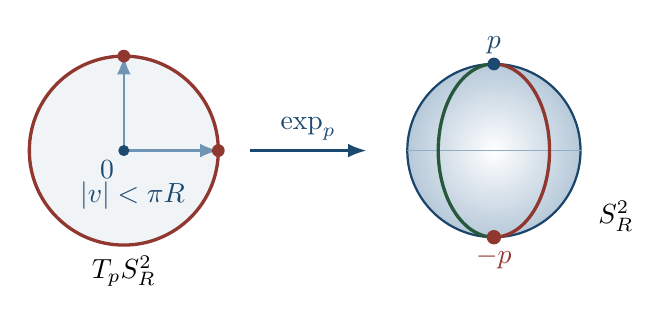
\begin{tikzpicture}[>=Latex,scale=1]
  \fill[manifoldblue!7] (-2.55,0) circle (1.20);
  \draw[manifoldred!85!black,very thick] (-2.55,0) circle (1.20);
  \draw[manifoldblue!65,thick,->] (-2.55,0)--(-1.35,0);
  \draw[manifoldblue!65,thick,->] (-2.55,0)--(-2.55,1.20);
  \fill[manifoldblue!80!black] (-2.55,0) circle (2pt)
       node[below left] {$0$};
  \fill[manifoldred!85!black] (-1.35,0) circle (2.3pt);
  \fill[manifoldred!85!black] (-2.55,1.20) circle (2.3pt);
  \node[manifoldblue!80!black] at (-2.44,-.57) {$|v|<\pi R$};
  \node at (-2.55,-1.53) {$T_pS_R^2$};
  \draw[->,thick,manifoldblue!80!black] (-.95,0)--(.53,0)
        node[midway,above] {$\exp_p$};
  \shade[inner color=white,outer color=manifoldblue!33]
       (2.15,0) circle (1.10);
  \draw[manifoldblue!75!black,thick] (2.15,0) circle (1.10);
  \draw[manifoldblue!50] (1.05,0)--(3.25,0);
  \draw[manifoldred!85!black,very thick]
       plot[domain=0:180,samples=60,variable=\u]
       ({2.15+1.10*sin(40)*sin(\u)},{1.10*cos(\u)});
  \draw[manifoldgreen!70!black,very thick]
       plot[domain=0:180,samples=60,variable=\u]
       ({2.15-1.10*sin(40)*sin(\u)},{1.10*cos(\u)});
  \fill[manifoldblue!80!black] (2.15,1.10) circle (2.3pt)
       node[above] {$p$};
  \fill[manifoldred!85!black] (2.15,-1.10) circle (2.6pt)
       node[below] {$-p$};
  \node at (3.70,-.83) {$S_R^2$};
\end{tikzpicture}
\caption{Na sferze okrąg $|v|=\pi R$ w przestrzeni stycznej
przechodzi przez $\exp_p$ w jeden punkt $-p$.
Wnętrze koła jest obszarem jednoznacznych geodezyjnych
minimalnych; dwa półokręgi na sferze pokazują
różne drogi do antypody.}
\label{fig:ciecie-sfera}
\end{figure}

\begin{przyklad}[Prostokątny płaski torus]
\label{prz:ciecie-torus}
Niech $a,b>0$ i
$T^2_{a,b}=\R^2/(a\Z\times b\Z)$ z metryką
odziedziczoną z płaszczyzny. Pisząc $[x,y]$
na klasę punktu $(x,y)$, przyjmijmy $p=[0,0]$.
Geodezyjne są rzutami prostych, więc
$\exp_p(v_1,v_2)=[v_1,v_2]$.
Każda krzywa z $p$ do $[x,y]$ podnosi się do
krzywej z $(0,0)$ do pewnego
$(x+ma,y+nb)$, $m,n\in\Z$, o tej samej długości.
Euklidesowa nierówność z
Przykładu~\ref{prz:geodezyjne-euklidesowe}
i rzut odpowiedniego odcinka dają dokładnie
\begin{equation}\label{eq:odleglosc-torus-ciecie}
 d_g(p,[x,y])
 =\min_{m,n\in\Z}
   \sqrt{(x+ma)^2+(y+nb)^2}.
\end{equation}
Minimum istnieje, bo długości wektorów kratowych
rosną do nieskończoności.

Wśród wszystkich reprezentantów klasy najbliższy
zera leży w prostokącie
$V=[-a/2,a/2]\times[-b/2,b/2]$.
We wnętrzu jest jedyny: każdą współrzędną
osobno wybieramy najbliższą zeru modulo $a$
lub modulo $b$. Na boku są dwa równoodległe
reprezentanty, a w narożniku cztery.
Dlatego promień w kierunku jednostkowym
$u=(u_1,u_2)$ jest minimalny dokładnie do
pierwszego spotkania z brzegiem $V$:
\[
 c_p(u)=
 \min\left\{\frac{a}{2|u_1|},
             \frac{b}{2|u_2|}\right\},
 \qquad \frac1{0}:=\infty.
\]
Zbiór cięcia to obraz brzegu prostokąta:
\[
 \operatorname{Cut}(p)
 =\{[a/2,y]:y\in\R\}
   \cup\{[x,b/2]:x\in\R\},
 \qquad
 \operatorname{inj}(p)
 =\operatorname{inj}(T^2_{a,b})
 =\frac12\min(a,b).
\]
Każda z obu krzywych tworzących zbiór cięcia
jest okręgiem; przecinają się w jednej
klasie $[a/2,b/2]$.
W punkcie ogólnym każdego z nich są dwie
minimalne geodezyjne od $p$, a w ich przecięciu
cztery. Różniczka $\dd(\exp_p)_v$ jest wszędzie
odwracalna, bo rzut $\R^2\to T^2_{a,b}$
jest lokalną izometrią. Torus nie ma więc
punktów sprzężonych: tutaj cięcie wynika
wyłącznie z wielości minimalnych geodezyjnych.
\end{przyklad}

\begin{figure}[htbp]
\centering
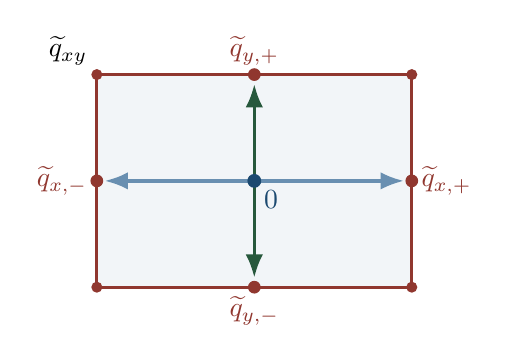
\begin{tikzpicture}[>=Latex,scale=1]
  \fill[manifoldblue!6] (-2,-1.35) rectangle (2,1.35);
  \draw[manifoldred!85!black,very thick]
       (-2,-1.35) rectangle (2,1.35);
  \draw[manifoldblue!68,very thick,->] (0,0)--(1.90,0);
  \draw[manifoldblue!68,very thick,->] (0,0)--(-1.90,0);
  \draw[manifoldgreen!70!black,very thick,->] (0,0)--(0,1.23);
  \draw[manifoldgreen!70!black,very thick,->] (0,0)--(0,-1.23);
  \fill[manifoldblue!80!black] (0,0) circle (2.5pt)
       node[below right] {$0$};
  \fill[manifoldred!85!black] (2,0) circle (2.3pt)
       node[right] {$\widetilde q_{x,+}$};
  \fill[manifoldred!85!black] (-2,0) circle (2.3pt)
       node[left] {$\widetilde q_{x,-}$};
  \fill[manifoldred!85!black] (0,1.35) circle (2.3pt)
       node[above] {$\widetilde q_{y,+}$};
  \fill[manifoldred!85!black] (0,-1.35) circle (2.3pt)
       node[below] {$\widetilde q_{y,-}$};
  \foreach \x in {-2,2}
    \foreach \y in {-1.35,1.35}
      \fill[manifoldred!85!black] (\x,\y) circle (2pt);
  \node[above left] at (-2,1.35) {$\widetilde q_{xy}$};
\end{tikzpicture}
\caption{Komórka najbliższych reprezentantów w nakryciu
płaskiego torusa: ma szerokość $a$ i wysokość $b$.
Przeciwległe boki są utożsamione:
pary $\widetilde q_{x,\pm}$ i $\widetilde q_{y,\pm}$
mają po jednym obrazie na torusie,
a cztery narożniki także jeden wspólny obraz.
Czerwony brzeg rzutuje się na dwa okręgi zbioru cięcia.}
\label{fig:ciecie-torus}
\end{figure}

Porównanie jest pouczające: na sferze granica
jednoznaczności i pierwszy punkt sprzężony wypadają
w odległości $\pi R$, a na płaskim torusie sama
topologia ogranicza promień injektywności
do połowy krótszego okresu kratowego.
Więcej o zbiorze cięcia i jego związku
z promieniem injektywności podaje
\href{https://www.math.ucla.edu/~petersen/RG.pdf}
{P.~Petersen, \emph{Riemannian Geometry}, rozdział 5}.

\section{Schwarzschild i Kerr: geodezyjne czasoprzestrzeni}
\label{sec:geodezyjne-schwarzschild-kerr}

Obie metryki z \eqref{eq:schwarzschild} i
\eqref{eq:kerr} są \emph{lorentzowskie}.
Równanie~\eqref{eq:geodezyjna-ode} i $\exp_p$
nadal mają sens lokalnie, podobnie jak ich
dowody z ODE. Nie ma jednak dodatniej normy
$\sqrt{g(v,v)}$ dla wszystkich wektorów,
więc odległość $d_g$ z Rozdziału~\ref{ch:metryka-riemannowska},
lemat o minimalności długości i twierdzenie
Hopfa--Rinowa nie stosują się do \emph{całej}
czasoprzestrzeni.

Dla czasopodobnej krzywej z parametrem $\lambda$
jej \emph{czas własny} jest równy
\begin{equation}\label{eq:czas-wlasny}
 \tau(\gamma)=\int\sqrt{-g(\dot\gamma,\dot\gamma)}
                    \,\dd\lambda.
\end{equation}
Przy sygnaturze $(-,+,+,+)$ czasopodobna
geodezyjna między dostatecznie bliskimi
punktami \emph{maksymalizuje} czas własny
wśród przyszłościowych krzywych czasopodobnych o tych samych
końcach, zawartych w odpowiednio małym otoczeniu normalnym. W płaskim modelu
$g=-\dd t^2+|\dd x|^2$, po przejściu do
układu spoczynkowego końców, dla
$x(a)=x(b)$ mamy wprost
\[
 \tau(\alpha)=\int_a^b
 \sqrt{\dot t^2-|\dot x|^2}\,\dd\lambda
 \leq\int_a^b\dot t\,\dd\lambda=t(b)-t(a),
\]
z równością dla prostej o stałym $x$.
W zakrzywionej czasoprzestrzeni ten argument
ma lokalną wersję. Dowód lematu
Gaussa~\ref{lem:gaussa-exp} używa jedynie
zgodności z metryką i braku torsji, więc
działa również dla metryki lorentzowskiej.
Wybieramy orientację czasu w małym otoczeniu normalnym $U$
punktu $p$. Możemy je zmniejszyć tak, aby istniała współrzędna
$x^0$ z $\dd x^0$ dodatnią na wszystkich niezerowych
przyszłościowych wektorach przyczynowych. Wystarczy wybrać taką współrzędną
w $p$ i zachować czasopodobność jej gradientu przez ciągłość.

Dlaczego przyszłościowa krzywa czasopodobna wychodząca z $p$
i pozostająca w $U$ leży w obrazie przyszłego stożka?
Niech $Q(\exp_p v)=g_p(v,v)$ i $R_{\exp_p v}=\dd(\exp_p)_v(v)$.
Lemat Gaussa daje $\dd Q(W)=2g(R,W)$.
Początkowo krzywa leży w przyszłym stożku, gdyż
$\dd(\exp_p)_0=\id$ i jej początkowa prędkość jest czasopodobna.
Gdyby po raz pierwszy doszła do niezerowego punktu jego
świetlnego brzegu, mielibyśmy tam $Q=0$ i $Q'\geq0$.
Jednak $R$ jest wtedy niezerowym przyszłościowym wektorem
światłopodobnym, zatem $Q'=2g(R,\dot\alpha)<0$.
Ostatnia nierówność wynika w bazie lorentzowskiej z
$R=(r,\xi)$, $r=|\xi|>0$, i $\dot\alpha=(a,\eta)$,
$a>|\eta|$: $-ra+\xi\cdot\eta<0$.
Powrót do wierzchołka $p$ wyklucza ścisły wzrost $x^0$.
Krzywa pozostaje więc w przyszłym stożku.

We wnętrzu tego stożka
piszemy $v=\tau u$, gdzie $g_p(u,u)=-1$,
$\tau>0$. Ortogonalne do czasopodobnego
kierunku $u$ wektory mają dodatni kwadrat
normy. Lemat Gaussa daje więc w tych
współrzędnych schemat metryki
$g=-\dd\tau^2+h_{ab}(\tau,u)\dd u^a\dd u^b$
z dodatnio określonym $h_{ab}$.
Radialne pole $\partial_\tau$ jest przyszłościowe,
jednostkowe i czasopodobne. Dla przyszłościowej krzywej
czasopodobnej mamy więc $\dot\tau=-g(\partial_\tau,\dot\alpha)>0$ i
\[
 \sqrt{-g(\dot\alpha,\dot\alpha)}
 =\sqrt{(\dot\tau)^2-h_{ab}\dot u^a\dot u^b}
 \leq\dot\tau.
\]
Całkujemy od dodatniego parametru i przechodzimy do początku
krzywej, gdzie $\tau\to0$. Dostajemy $\tau(\alpha)
\leq\tau(q)$; radialna geodezyjna osiąga
równość. Tym samym lokalna maksymalność
dotyczy dróg mieszczących się w takim
otoczeniu przy ustalonych końcach.
Nie jest to twierdzenie o \emph{minimalizowaniu}
riemannowskiej odległości. Dla geodezyjnych
światłopodobnych czas własny wynosi zero.

\begin{przyklad}[Ruch w metryce Schwarzschilda]
\label{prz:geodezyjne-schwarzschild}
Pracujemy w obszarze $r>2M$, $M>0$. Z uwagi na symetrię
sferyczną możemy wybrać płaszczyznę ruchu $\theta=\pi/2$:
obracamy początkowe dane przestrzenne do jednej płaszczyzny
przez środek. Odbicie względem niej jest izometrią
zachowującą te dane, więc jednoznaczność geodezyjnej
utrzymuje ruch w tej płaszczyźnie.
Na geodezyjnej z parametrem afinicznym
Lagrangian $\mathcal L=\tfrac12g_{\mu\nu}
\dot x^\mu\dot x^\nu$ nie zależy od $t,\phi$.
Równania Eulera--Lagrange'a dają więc
stałe wielkości
\begin{equation}\label{eq:stale-schwarzschild}
 E=f(r)\dot t,\qquad L=r^2\dot\phi,
 \qquad f(r)=1-\frac{2M}{r}.
\end{equation}
Niech $g(\dot\gamma,\dot\gamma)=-\kappa$:
$\kappa=1$ dla czasopodobnej geodezyjnej
parametryzowanej czasem własnym i $\kappa=0$
dla światłopodobnej. Podstawienie
$\dot t=E/f$, $\dot\phi=L/r^2$ do metryki daje
\begin{equation}\label{eq:radialne-schwarzschild}
 -\kappa=-\frac{E^2}{f}+\frac{\dot r^2}{f}
                   +\frac{L^2}{r^2}
 \quad\Longleftrightarrow\quad
 \dot r^2+f\left(\kappa+\frac{L^2}{r^2}\right)=E^2.
\end{equation}
To pierwsza całka równania radialnego. W punktach zwrotnych
nie wolno dzielić jej pochodnej przez $\dot r=0$.
Pełne równanie geodezyjnej, po wstawieniu symboli
z \eqref{eq:gamma-schwarzschild} i powyższej pierwszej całki, daje
\[
 \ddot r=-\tfrac12 f'\left(\kappa+\frac{L^2}{r^2}\right)
                  +\frac{fL^2}{r^3}
        =-\tfrac12\frac{\dd}{\dd r}
                    \left[f\left(\kappa+\frac{L^2}{r^2}\right)\right].
\]
Ten wzór obowiązuje także przy $\dot r=0$.
Przy $\kappa=0$, $L\ne0$ stały promień
orbity światłopodobnej wymaga $\dot r=0$
i pochodnej potencjału
$V(r)=L^2(1-2M/r)/r^2$ równej zeru.
Ponieważ
$V'(r)=2L^2(3M-r)/r^4$, dostajemy
$r=3M$ i z \eqref{eq:radialne-schwarzschild}
$E^2=L^2/(27M^2)$. To przykład geodezyjnej,
która może krążyć po sferze fotonowej;
nie jest to okrąg minimalizujący długość
w sensie riemannowskim.
\end{przyklad}

\begin{figure}[htbp]
\centering
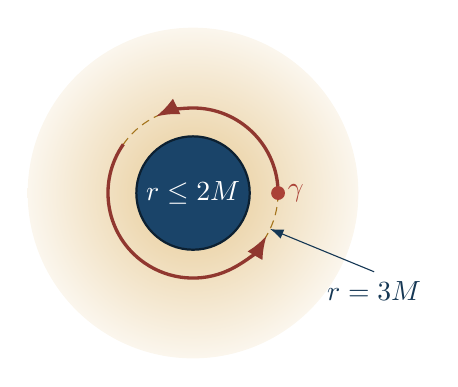
\begin{tikzpicture}[>=Latex,scale=1]
  \shade[inner color=manifoldgold!50,outer color=manifoldgold!8]
       (0,0) circle (2.10);
  \fill[manifoldblue!75!black] (0,0) circle (.72);
  \draw[manifoldblue!35!black,thick] (0,0) circle (.72);
  \draw[manifoldgold!80!black,densely dashed]
       (0,0) circle (1.08);
  \draw[manifoldred!85!black,very thick,->]
       (0:1.08) arc[start angle=0,end angle=116,radius=1.08];
  \draw[manifoldred!85!black,very thick,->]
       (145:1.08) arc[start angle=145,end angle=330,radius=1.08];
  \fill[manifoldred] (1.08,0) circle (2.5pt)
       node[right] {$\gamma$};
  \draw[manifoldblue!60!black,->]
       (2.30,-1.0)--(-25:1.08)
       node[pos=0,below] {$r=3M$};
  \node[white] at (0,0) {$r\leq2M$};
\end{tikzpicture}
\caption{Schemat rzutu na współrzędne $(r,\phi)$ równikowej geodezyjnej światłopodobnej Schwarzschilda o stałym $r=3M$. Ciemny dysk oznacza $r\leq2M$ w tym rysunku współrzędnych; okrąg $r=3M$ nie przedstawia geodezyjnej metryki indukowanej na przekroju przestrzennym.}
\label{fig:geodezyjna-schwarzschild-foton}
\end{figure}

\begin{przyklad}[Ruch równikowy w metryce Kerra]
\label{prz:geodezyjne-kerr}
Przyjmujemy $M>0$, $|a|\leq M$ i $r>r_+=M+\sqrt{M^2-a^2}$.
Płaszczyzna $\theta=\pi/2$ jest niezmiennicza
przez symetrię odbicia $\theta\mapsto\pi-\theta$:
geodezyjna startująca na niej ze
$\dot\theta=0$ na niej pozostaje.
Niech $E=-p_t$, $L=p_\phi$, gdzie
$p_\mu=g_{\mu\nu}\dot x^\nu$; są to stałe,
bo metryka nie zależy od $t,\phi$.
W tej płaszczyźnie $\Sigma=r^2$. Oznaczmy
\[
 A=\dot t-a\dot\phi,
 \qquad B=(r^2+a^2)\dot\phi-a\dot t.
\]
Z postaci \eqref{eq:kerr} przez różniczkowanie
Lagrangianu względem $\dot t,\dot\phi$
otrzymujemy
\[
 E=\frac{\Delta A+aB}{r^2},
 \qquad
 L=\frac{a\Delta A+(r^2+a^2)B}{r^2}.
\]
Odejmujemy $aE$ od $L$: dostajemy
$B=L-aE$, a stąd $\Delta A=P(r)$,
gdzie $P(r)=E(r^2+a^2)-aL$.
Warunek $g(\dot\gamma,\dot\gamma)=-\kappa$
daje po pomnożeniu przez $r^2\Delta$
\begin{equation}\label{eq:radialne-kerr}
 r^4\dot r^2=P(r)^2
        -\Delta\bigl(\kappa r^2+(L-aE)^2\bigr),
 \qquad \kappa\in\{0,1\}.
\end{equation}
Możemy również odzyskać pozostałe pochodne:
\begin{equation}\label{eq:tphi-kerr}
 r^2\dot t=\frac{r^2+a^2}{\Delta}P+a(L-aE),
 \qquad
 r^2\dot\phi=\frac a\Delta P+(L-aE).
\end{equation}
Wzory dotyczą geodezyjnych równikowych;
poza tą płaszczyzną ruch wymaga jeszcze
jednej stałej związanej z kątem $\theta$.
Przy $a=0$ równanie~\eqref{eq:radialne-kerr}
redukuje się do~\eqref{eq:radialne-schwarzschild}.
Także tutaj pierwsza całka radialna nie zastępuje pełnego
równania geodezyjnej przy poszukiwaniu rozwiązań stałych
lub przedłużaniu przez punkty zwrotne.

Dla kołowej geodezyjnej równikowej o
$\Omega=\dot\phi/\dot t$ i $\dot r=0$
radialne równanie geodezyjnej daje
\[
 \partial_rg_{tt}+2\Omega\partial_rg_{t\phi}
                 +\Omega^2\partial_rg_{\phi\phi}=0.
\]
Na równiku
$g_{tt}=-1+2M/r$,
$g_{t\phi}=-2Ma/r$,
$g_{\phi\phi}=r^2+a^2+2Ma^2/r$;
po pomnożeniu równania przez $r^2/2$
otrzymujemy
\[
 -M+2Ma\Omega+(r^3-Ma^2)\Omega^2=0,
 \qquad
 \Omega_\pm=\frac{\pm\sqrt M}{r^{3/2}\pm a\sqrt M}.
\]
To \emph{kandydaci} na orbity kołowe: dla
czasopodobnej trzeba ponadto sprawdzić
$g(\partial_t+\Omega_\pm\partial_\phi,
   \partial_t+\Omega_\pm\partial_\phi)<0$
w rozważanym promieniu. Przy $a=0$
dostajemy $\Omega_\pm=\pm\sqrt{M/r^3}$.
\end{przyklad}

\begin{figure}[htbp]
\centering
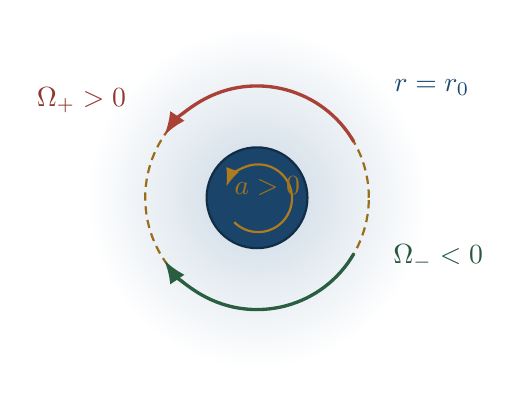
\begin{tikzpicture}[>=Latex,scale=1]
  \shade[inner color=manifoldblue!24,outer color=white]
       (0,0) circle (2.16);
  \fill[manifoldblue!75!black] (0,0) circle (.64);
  \draw[manifoldblue!50!black,thick] (0,0) circle (.64);
  \draw[manifoldgold!75!black,thick,densely dashed]
       (0,0) circle (1.42);
  \draw[manifoldred,very thick,->]
       (30:1.42) arc[start angle=30,end angle=146,radius=1.42];
  \draw[manifoldgreen!75!black,very thick,->]
       (330:1.42) arc[start angle=330,end angle=214,radius=1.42];
  \node[manifoldred!85!black] at (-2.23,1.24)
       {$\Omega_+>0$};
  \node[manifoldgreen!70!black] at (2.30,-.75)
       {$\Omega_-<0$};
  \draw[manifoldgold!85!black,thick,->]
       (-.29,-.31) arc[start angle=225,end angle=520,radius=.43];
  \node[manifoldgold!80!black] at (.13,.15) {$a>0$};
  \node[manifoldblue!80!black] at (2.22,1.40)
       {$r=r_0$};
\end{tikzpicture}
\caption{Schemat rzutu na płaszczyznę równikową dwóch kierunków kołowej geodezyjnej Kerra przy dodatnim $a$ i odpowiednio dużym $r_0$. Strzałki $\Omega_+$ i $\Omega_-$ oznaczają ruch zgodny z obrotem i przeciwny. Ciemny obszar schematycznie zaznacza wnętrze $r_+$, a okrąg przerywany jest stałym $r_0$ we współrzędnych Boyera--Lindquista; nie jest to zanurzenie zakrzywionej czasoprzestrzeni.}
\label{fig:geodezyjna-kerr-kolowa}
\end{figure}

\subsection*{Riemannowskie przekroje przestrzenne: co w nich minimalizuje?}
\label{subsec:przekroje-przestrzenne-geodezyjne}

Można osobno wybrać przekrój $t=\mathrm{const}$
i jego \emph{indukowaną metrykę riemannowską}
$h$. To inny problem geometryczny niż
geodezyjne pełnej czasoprzestrzeni.
Rysunek~\ref{fig:geodezyjne-przestrzen-czas} zestawia
przestrzenną długość z czasem własnym; prawe okno
pokazuje płaską czasoprzestrzeń, aby oddzielić te
dwa rodzaje pomiaru przed obliczeniami metryk
Schwarzschilda i Kerra.

\begin{figure}[H]
\centering
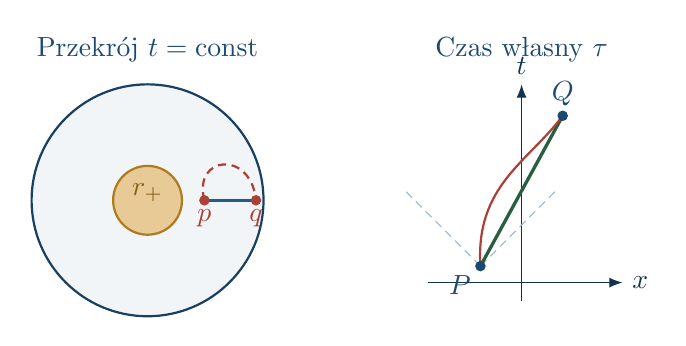
\begin{tikzpicture}[>=Latex,scale=.95]
  \fill[manifoldblue!6] (-2.9,0) circle (1.55);
  \draw[manifoldblue!70!black,thick] (-2.9,0) circle (1.55);
  \fill[manifoldgold!48] (-2.9,0) circle (.46);
  \draw[manifoldgold!85!black,thick] (-2.9,0) circle (.46);
  \draw[manifoldblue,very thick] (-2.9,0) ++(.76,0)--++(.69,0);
  \fill[manifoldred] (-2.14,0) circle (2pt) node[below] {$p$};
  \fill[manifoldred] (-1.45,0) circle (2pt) node[below] {$q$};
  \draw[manifoldred,thick,densely dashed]
    (-2.14,0) .. controls (-2.3,.6) and (-1.52,.68) .. (-1.45,0);
  \node[manifoldgold!65!black] at (-2.9,.1) {$r_+$};
  \node[manifoldblue!80!black] at (-2.9,2.02) {Przekrój $t=\mathrm{const}$};
  \draw[manifoldblue!55!black,->] (2.1,-1.35)--(2.1,1.55) node[above] {$t$};
  \draw[manifoldblue!55!black,->] (.85,-1.1)--(3.45,-1.1) node[right] {$x$};
  \coordinate (lp) at (1.55,-.88);
  \coordinate (lq) at (2.65,1.13);
  \draw[manifoldblue!45,densely dashed] (lp)--++(-1.02,1.02);
  \draw[manifoldblue!45,densely dashed] (lp)--++(1.02,1.02);
  \draw[manifoldgreen!75!black,very thick] (lp)--(lq);
  \draw[manifoldred,thick] (lp)
    .. controls (1.48,.20) and (2.20,.52) .. (lq);
  \fill[manifoldblue!80!black] (lp) circle (2pt) node[below left] {$P$};
  \fill[manifoldblue!80!black] (lq) circle (2pt) node[above] {$Q$};
  \node[manifoldblue!80!black] at (2.1,2.02) {Czas własny $\tau$};
\end{tikzpicture}
\caption{Po lewej odcinek radialny minimalizuje długość w riemannowskim przekroju przestrzennym. Po prawej prosta czasopodobna maksymalizuje czas własny między ustalonymi zdarzeniami w płaskiej czasoprzestrzeni. Schemat nie przedstawia zanurzenia metryki Kerra.}
\label{fig:geodezyjne-przestrzen-czas}
\end{figure}

W zewnętrznym obszarze Schwarzschilda
\[
 h_{\mathrm{Sch}}=f^{-1}\dd r^2
    +r^2(\dd\theta^2+\sin^2\theta\,\dd\phi^2).
\]
Na równiku krzywa o stałych $\theta=\pi/2$
i $\phi$ oraz zmiennym $r$ ma długość
\begin{equation}\label{eq:radialna-przestrzenna-schwarz}
 \ell_{\mathrm{Sch}}(r_0,r_1)
  =\left|\int_{r_0}^{r_1}
               \frac{\dd r}{\sqrt{1-2M/r}}\right|.
\end{equation}
Dowolna droga w tym przekroju między punktami
o tych samych kątach ma długość co najmniej
$\int|\dot r|/\sqrt f\,\dd s\geq\ell_{\mathrm{Sch}}$;
monotoniczna krzywa radialna osiąga równość.

Dla Kerra na $t=\mathrm{const}$ i $\theta=\pi/2$
składowe metryki indukowanej wynoszą
\[
 h_{rr}=\frac{r^2}{\Delta},\qquad
 h_{\phi\phi}=r^2+a^2+\frac{2Ma^2}{r}.
\]
Stąd radialna długość ma wzór
\begin{equation}\label{eq:radialna-przestrzenna-kerr}
 \ell_{\mathrm K}(r_0,r_1)
   =\left|\int_{r_0}^{r_1}
                   \frac r{\sqrt\Delta}\,\dd r\right|.
\end{equation}
Ta droga też jest najkrótsza w \emph{tym przekroju}
między równikowymi punktami o tych samych
kątach: dla dowolnej drogi $\Sigma\geq r^2$
i $h_{rr}=\Sigma/\Delta$, zatem
$|\dot\alpha|_h\geq r|\dot r|/\sqrt\Delta$.
Po scałkowaniu dostajemy dolne ograniczenie
\eqref{eq:radialna-przestrzenna-kerr}, osiągane
przez krzywą radialną na równiku. Wobec
Wniosku~\ref{cor:minimalna-geodezyjna}
obie radialne krzywe, po parametryzacji
długością łuku, są geodezyjnymi swoich
\emph{przestrzennych} metryk $h$.

Te zewnętrzne przekroje $r>r_+$ nie są
automatycznie zupełne. Dla Schwarzschilda
całka~\eqref{eq:radialna-przestrzenna-schwarz}
do pominiętego brzegu $r=2M$ jest skończona.
Dla Kerra o $|a|<M$ mamy
$\Delta=(r-r_+)(r-r_-)$, $r_-<r_+$,
więc całka~\eqref{eq:radialna-przestrzenna-kerr}
do $r_+$ również jest skończona.
Wynika to z zachowania całkowanego wyrażenia
jak $C/\sqrt{r-r_+}$ blisko horyzontu.
Horyzont nie należy do opisywanego przekroju;
ciąg punktów na ustalonym promieniu równikowym,
z $r\downarrow r_+$, jest w nim ciągiem Cauchy'ego bez granicy. Nie przeczy
to Hopfowi--Rinowowi, ponieważ jego hipoteza
zupełności tutaj nie zachodzi.

\par\smallskip
{\footnotesize\noindent\emph{Dalsza lektura:}
\href{https://math.uchicago.edu/~may/REU2016/REUPapers/Spiegel.pdf}
{dowód Hopfa--Rinowa},
\href{https://www.math.toronto.edu/mein/teaching/LectureNotes/rieall.pdf}
{geodezyjne i współrzędne normalne},
\href{https://math.uchicago.edu/~dannyc/courses/kleinian_groups_2015/kleinian_groups.pdf}
{geodezyjne w modelach hiperbolicznych},
\href{https://ocw.mit.edu/courses/8-033-relativity-fall-2006/bc94629f28eae7b92641aecbc4bf8502_lecture21_bh1.pdf}
{orbity Schwarzschilda w notatkach MIT},
\href{https://sites.science.oregonstate.edu/coursewikis/GGR/book/content/kerr}
{metryka Kerra}.\par}

\chapter{Krzywizna: od transportu równoległego do tensorów}
\label{ch:krzywizna}
\index{krzywizna}

Co właściwie znaczy, że przestrzeń jest zakrzywiona?
Możemy wykonać pomiary \emph{wewnątrz} niej: poprowadzić
geodezyjne (odpowiedniki prostych), zmierzyć obwód małego
okręgu albo przenieść wektor wzdłuż zamkniętej drogi.
Na płaszczyźnie mały okrąg o promieniu $r$ ma obwód
$2\pi r$, a wektor po obejściu pętli wraca bez obrotu.
Na sferze obwód jest mniejszy, a na płaszczyźnie
hiperbolicznej większy; transport po pętli może obrócić
wektor. \emph{Krzywizna} opisuje właśnie te odchylenia
od geometrii euklidesowej. Bardzo małe otoczenie
każdego punktu wygląda w pierwszym przybliżeniu
płasko; krzywizna ujawnia się w kolejnych wyrazach
rachunku dla małych odległości.

Nie chodzi o samo wygięcie w większej przestrzeni.
Mały fragment walca w $\R^3$ można rozwinąć na płaszczyznę
bez rozciągania, więc jego wewnętrzna krzywizna jest
zerowa. Definicja przez metrykę i koneksję ma sens
także wtedy, gdy nie przedstawiamy rozmaitości jako
powierzchni zanurzonej w $\R^3$.

W rozdziale o koneksjach porównywaliśmy wektory w różnych
punktach za pomocą transportu równoległego. Pytanie,
czy wynik zależy od drogi, prowadzi do tensora Riemanna:
pełnego opisu krzywizny w punkcie. Krzywizna sekcyjna
bada jedną wybraną płaszczyznę styczną; na powierzchni
jest to krzywizna Gaussa. Tensor Ricciego sumuje
krzywizny płaszczyzn zawierających wybrany kierunek,
a krzywizna skalarna zbiera informację ze wszystkich
kierunków. Poniżej pokażemy, co te sumy mówią o
objętości małych obszarów.

Przez większość rozdziału $(M,g)$ jest rozmaitością
\emph{riemannowską}, a $\nabla$ jej koneksją Leviego-Civity
z Twierdzenia~\ref{thm:levi-civita}. Domyślnie rozmaitości
nie mają brzegu; powierzchnie z brzegiem i narożnikami
wprowadzimy osobno przy twierdzeniu Gaussa--Bonneta. W przykładach
Schwarzschilda i Kerra $g$ ma sygnaturę lorentzowską.
Te same wzory tensorowe nadal obowiązują, lecz wtedy
nie każda płaszczyzna ma określoną krzywiznę sekcyjną,
a ślad z metryką zawiera znaki ujemne.

\section{Co mierzy krzywizna? Tensor Riemanna}

\begin{definicja}[konwencja znaku]\label{def:tensor-krzywizny}
\index{konwencja znaku@konwencja znaku}
Niech $X,Y,Z$ będą polami wektorowymi. Definiujemy
\begin{equation}\label{eq:riemann-def}
 R(X,Y)Z=\nabla_X\nabla_YZ-\nabla_Y\nabla_XZ
                        -\nabla_{[X,Y]}Z,
 \qquad
 \mathcal R(X,Y,Z,W)=g(R(X,Y)Z,W).
\end{equation}
Symbol $R$ nazywamy \emph{operatorem krzywizny}, a
$\mathcal R$ \emph{tensorem Riemanna} o wszystkich
indeksach opuszczonych. Ta konwencja daje dodatnią
krzywiznę sekcyjną zwykłej sfery. W literaturze spotyka
się także przeciwny znak $R$; przy porównywaniu wzorów
trzeba zawsze sprawdzić definicję.
\end{definicja}

Pierwsze dwa składniki mierzą różnicę między różniczkowaniem
najpierw w kierunku $Y$, a potem $X$, oraz w przeciwnej
kolejności. Człon $\nabla_{[X,Y]}Z$ usuwa różnicę pochodzącą
tylko z tego, że same pola $X,Y$ nie muszą komutować.
W efekcie $R(X,Y)Z$ zależy \emph{wyłącznie} od wartości
$X,Y,Z$ w danym punkcie.

\begin{stwierdzenie}[tensorowość i współrzędne]
\label{prop:riemann-tensorowy}
Wyrażenie $R$ jest liniowe nad $C^\infty(M)$ w każdym
z trzech argumentów. Jeżeli
$\nabla_{\partial_i}\partial_j=\Gamma^a_{ij}\partial_a$,
to przy umowie
$R(\partial_i,\partial_j)\partial_b
 =R^a{}_{b i j}\partial_a$ mamy
\begin{equation}\label{eq:riemann-wspolrzedne}
 R^a{}_{b i j}
 =\partial_i\Gamma^a_{j b}-\partial_j\Gamma^a_{i b}
  +\Gamma^a_{i c}\Gamma^c_{j b}
  -\Gamma^a_{j c}\Gamma^c_{i b}.
\end{equation}
W szczególności tensor krzywizny zawiera pochodne
współczynników koneksji, a więc drugie pochodne metryki.
\end{stwierdzenie}

\begin{proof}
Dla dowolnej funkcji $f$ reguły koneksji i nawiasu dają
$\nabla_{fX}Y=f\nabla_XY$ oraz
$[fX,Y]=f[X,Y]-Y(f)X$. Zatem
\[
 \begin{split}
 R(fX,Y)Z
 &=f\nabla_X\nabla_YZ-\nabla_Y(f\nabla_XZ)
        -\nabla_{f[X,Y]-Y(f)X}Z\\
 &=fR(X,Y)Z-Y(f)\nabla_XZ+Y(f)\nabla_XZ
  =fR(X,Y)Z.
 \end{split}
\]
Antysymetria $R(X,Y)=-R(Y,X)$ daje to samo w drugim
argumencie. W trzecim argumencie rozwińmy
$\nabla_Y(fZ)=Y(f)Z+f\nabla_YZ$ i odpowiedni wyraz
z zamienionymi $X,Y$. Składniki zawierające pochodne
samego $Z$ znoszą się parami, natomiast pozostały
współczynnik przy $Z$ wynosi
$X(Yf)-Y(Xf)-[X,Y]f=0$. Dlatego $R(X,Y)(fZ)=fR(X,Y)Z$.

Ponieważ $[\partial_i,\partial_j]=0$, wstawiamy pola
współrzędnych do~\eqref{eq:riemann-def}:
\[
 \nabla_{\partial_i}(\Gamma^c_{jb}\partial_c)
 =(\partial_i\Gamma^a_{jb}
       +\Gamma^c_{jb}\Gamma^a_{ic})\partial_a.
\]
Po odjęciu wyrażenia z $i,j$ zamienionymi miejscami
otrzymujemy~\eqref{eq:riemann-wspolrzedne}.
\end{proof}

\begin{uwaga}[mały obwód i transport]\label{uwaga:holonomia}
Wybierzmy współrzędne normalne w $p$ i niezależne
$X_p,Y_p\in T_pM$. Obraz brzegu równoległoboku
$0,\varepsilon X_p,\varepsilon(X_p+Y_p),\varepsilon Y_p$
przez mapę normalną jest rzeczywistą zamkniętą pętlą.
Jej transport $P_\varepsilon:T_pM\to T_pM$ spełnia
\[
 P_\varepsilon v=v-\varepsilon^2R(X_p,Y_p)v+O(\varepsilon^3).
\]
Uzasadnijmy znak i rząd reszty. W trywializacji współrzędnych
piszemy $\Gamma_i=(\Gamma^a_{ib})_{a,b}$. Równanie
transportu ma postać $\dot V=-\Gamma_i(x)\dot x^iV$.
Ponieważ $\Gamma_i(0)=0$, na całej małej pętli
$V=v+O(\varepsilon^2)$, a więc
\[
 P_\varepsilon v-v
 =-\oint\Gamma_i(x)\,\dd x^i\,v+O(\varepsilon^4)
 =-\varepsilon^2(\partial_X\Gamma_Y-\partial_Y\Gamma_X)_p v
     +O(\varepsilon^3).
\]
Ostatnia równość wynika z liniowego rozwinięcia $\Gamma$;
składniki kwadratowe dają po całkowaniu $O(\varepsilon^3)$.
W punkcie $p$ iloczyny $\Gamma_i\Gamma_j$ znikają,
więc nawias jest macierzą $R(X_p,Y_p)$.
Odwrócenie obiegu zmienia znak głównego wyrazu.
Pole równoległoboku jest asymptotycznie równe
$\varepsilon^2|X_p\wedge Y_p|$; aby mówić o zmianie
\emph{na jednostkę pola}, dzielimy również przez
$|X_p\wedge Y_p|$ (dla pary ortonormalnej wynosi ono $1$).
Samo $\Gamma^a_{ij}\ne0$
nie świadczy o krzywiźnie: we współrzędnych biegunowych
płaskiej płaszczyzny symbole Christoffela są niezerowe,
ale wszystkie składniki $R$ znikają.
\end{uwaga}

\begin{figure}[htbp]
\centering
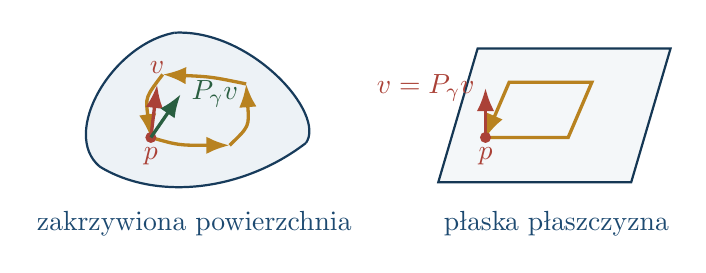
\begin{tikzpicture}[>=Latex,scale=1]
  \fill[manifoldblue!8] (-3.2,-.65)
    .. controls (-2.5,-1.08) and (-1.4,-.98) .. (-.58,-.35)
    .. controls (-.32,.02) and (-1.28,1.10) .. (-2.25,1.05)
    .. controls (-3.05,.9) and (-3.7,-.23) .. cycle;
  \draw[manifoldblue!65!black,thick] (-3.2,-.65)
    .. controls (-2.5,-1.08) and (-1.4,-.98) .. (-.58,-.35);
  \draw[manifoldblue!65!black,thick] (-.58,-.35)
    .. controls (-.32,.02) and (-1.28,1.10) .. (-2.25,1.05);
  \draw[manifoldblue!65!black,thick] (-2.25,1.05)
    .. controls (-3.05,.9) and (-3.7,-.23) .. (-3.2,-.65);
  \coordinate (A) at (-2.55,-.28);
  \coordinate (B) at (-1.55,-.38);
  \coordinate (C) at (-1.34,.40);
  \coordinate (D) at (-2.40,.52);
  \draw[manifoldgold!90!black,very thick,->]
    (A) .. controls (-2.20,-.38) .. (B);
  \draw[manifoldgold!90!black,very thick,->]
    (B) .. controls (-1.30,-.14) .. (C);
  \draw[manifoldgold!90!black,very thick,->]
    (C) .. controls (-1.78,.49) .. (D);
  \draw[manifoldgold!90!black,very thick,->]
    (D) .. controls (-2.62,.23) .. (A);
  \fill[manifoldred] (A) circle (2pt) node[below] {$p$};
  \draw[manifoldred,very thick,->] (A)--++(.08,.67)
      node[above] {$v$};
  \draw[manifoldgreen!75!black,very thick,->]
       (A)--++(.38,.55)
      node[right] {$P_\gamma v$};
  \node[manifoldblue!80!black,align=center] at (-2,-1.37)
      {zakrzywiona powierzchnia};
  \fill[manifoldblue!5] (1.1,-.85)--(3.55,-.85)
       --(4.05,.85)--(1.6,.85)--cycle;
  \draw[manifoldblue!60!black,thick]
       (1.1,-.85)--(3.55,-.85)--(4.05,.85)--(1.6,.85)--cycle;
  \draw[manifoldgold!90!black,very thick,->]
       (1.7,-.28)--(2.75,-.28)--(3.05,.42)
       --(2.0,.42)--(1.7,-.28);
  \fill[manifoldred] (1.7,-.28) circle (2pt) node[below] {$p$};
  \draw[manifoldred,very thick,->] (1.7,-.28)--++(0,.63)
       node[left] {$v=P_\gamma v$};
  \node[manifoldblue!80!black] at (2.6,-1.37)
      {płaska płaszczyzna};
\end{tikzpicture}
\caption{Transport wektora wzdłuż małej pętli.
Na zakrzywionej powierzchni wektor może wrócić obrócony;
na płaszczyźnie euklidesowej wraca w tej samej postaci.
Strzałki i pętla są schematyczne.}
\label{fig:krzywizna-holonomia}
\end{figure}

\section{Symetrie tensora i krzywizna sekcyjna}

\begin{twierdzenie}[symetrie i pierwsza tożsamość Bianchiego]
\label{thm:symetrie-riemanna}
Dla koneksji Leviego-Civity zachodzą
\begin{align}\label{eq:symetrie-riemanna}
 \mathcal R(X,Y,Z,W)&=-\mathcal R(Y,X,Z,W)
                     =-\mathcal R(X,Y,W,Z),\\
 \mathcal R(X,Y,Z,W)&=\mathcal R(Z,W,X,Y),\notag\\
 R(X,Y)Z+R(Y,Z)X+R(Z,X)Y&=0.\notag
\end{align}
Ostatnia równość to \emph{pierwsza tożsamość Bianchiego}.
\end{twierdzenie}

\begin{proof}
Antysymetria w $X,Y$ wynika wprost z definicji.
Pozostałe tożsamości są punktowe, więc wolno obliczyć je
w wygodnych współrzędnych. Wybierzmy współrzędne normalne
w punkcie $p$: $\Gamma^a_{ij}(p)=0$ i
$\partial_k g_{ij}(p)=0$. Znikanie pierwszych pochodnych
metryki wynika tu ze zgodności $\nabla g=0$ i $\Gamma(p)=0$.
Korzystając ze wzoru na symbole Christoffela
\eqref{eq:christoffel-metryka} oraz
\eqref{eq:riemann-wspolrzedne}, dostajemy w $p$
\begin{equation}\label{eq:riemann-drugie-pochodne}
 \begin{split}
 \mathcal R_{ij k l}
 :=\mathcal R(\partial_i,\partial_j,\partial_k,\partial_l)
 =\frac12\bigl(&\partial_i\partial_k g_{jl}
      -\partial_i\partial_l g_{jk}\\
      &-\partial_j\partial_k g_{il}
      +\partial_j\partial_l g_{ik}\bigr)(p).
 \end{split}
\end{equation}
Wyrazy kwadratowe w $\Gamma$ znikają w $p$.
Pierwszą i ostatnią parę indeksów można zamienić
miejscami, bo pochodne mieszane komutują i $g_{ij}=g_{ji}$.
Zamiana indeksów wewnątrz którejkolwiek pary zmienia
znak. Wreszcie po dodaniu wzoru
\eqref{eq:riemann-drugie-pochodne} dla trójek
$(i,j,k)$, $(j,k,i)$ i $(k,i,j)$ każdy składnik
drugich pochodnych znosi się z innym. To daje tożsamość
Bianchiego po sparowaniu z dowolnym $W$.
Tensorowość pozwala przenieść wynik z bazy
współrzędnych na dowolne wektory i dowolny punkt.
\end{proof}

\begin{definicja}[krzywizna sekcyjna]\label{def:krzywizna-sekcyjna}
\index{krzywizna sekcyjna@krzywizna sekcyjna}
Niech $\sigma\subset T_pM$ będzie dwuwymiarową
płaszczyzną z bazą $u,v$. W przypadku riemannowskim
\begin{equation}\label{eq:krzywizna-sekcyjna}
 K_p(\sigma)
 =\frac{g(R(u,v)v,u)}{|u|^2|v|^2-g(u,v)^2}
 =\frac{\mathcal R(u,v,v,u)}{|u\wedge v|^2}.
\end{equation}
Mianownik jest kwadratem pola równoległoboku
rozpiętego przez $u,v$. Dla ortonormalnej bazy
$u,v$ po prostu $K_p(\sigma)=g(R(u,v)v,u)$.
W sygnaturze lorentzowskiej ten sam iloraz określamy
tylko dla płaszczyzn \emph{niezdegenerowanych},
czyli gdy wyznacznik macierzy Grama w mianowniku
jest różny od zera.
\end{definicja}

\begin{proof}[Dlaczego wzór nie zależy od wybranej bazy]
Przy zmianie bazy płaszczyzny macierzą $A$ licznik
zmienia się przez czynnik $(\det A)^2$.
Wynika to z dwuliniowości i antysymetrii tensora
$\mathcal R$ osobno w dwóch parach argumentów:
każda para działa jak pole zorientowanego
równoległoboku. Mianownik jest wyznacznikiem
macierzy Grama, która przechodzi w $A^{\mathsf T}GA$,
więc także mnoży się przez $(\det A)^2$.
Iloraz jest zatem własnością samej płaszczyzny.
\end{proof}

\begin{uwaga}[intuicja]\label{uwaga:intuicja-sekcyjna}
Krzywizna sekcyjna bada, jak geometria zachowuje się
w wybranych \emph{dwóch} kierunkach stycznych. Na
sferze geodezyjne wychodzące z punktu zwykle zbliżają
się względem modelu płaskiego; w przestrzeni
hiperbolicznej rozchodzą się szybciej. W przestrzeni
o wymiarze $n\geq3$ różne płaszczyzny przez ten sam
punkt mogą mieć różne krzywizny. Krzywizna powierzchni
ma tylko jedną taką płaszczyznę, czyli całe $T_pM$.
\end{uwaga}

\section{Krzywizna Gaussa i \texorpdfstring{Theorema Egregium}{Theorema Egregium}}

Dla powierzchni $M^2\subset\R^3$ można najpierw pomyśleć
o tym, jak wygina się ona w przestrzeni. Nie jest to jednak
to samo co krzywizna wynikająca z pomiarów długości
\emph{na samej powierzchni}. Walec wygina się w $\R^3$,
ale można go rozwinąć na płaszczyźnie bez rozciągania.

Wyobraźmy sobie okrąg złożony z punktów odległych
o tę samą małą \emph{długość geodezyjną} $r$ od $p$.
W trzech modelach jego obwód jest odpowiednio
\[
 \begin{array}{c|c|c}
 K=R^{-2}\text{ na }S_R^2 & K=0\text{ na }\R^2
                         & K=-1\text{ na }\mathbb H^2\\ \hline
 2\pi R\sin(r/R) & 2\pi r & 2\pi\sinh r
 \end{array}
\]
(na sferze bierzemy $r<\pi R$). Pierwszy obwód jest
mniejszy od $2\pi r$, trzeci większy. Dla dowolnej
gładkiej powierzchni zachodzi przy $r\downarrow0$
\begin{equation}\label{eq:gauss-maly-okrag}
 L_p(r)=2\pi r\left(1-\frac{K(p)}6r^2+O(r^3)\right).
\end{equation}
Tak można \emph{zmierzyć} znak i wartość $K(p)$ bez
oglądania powierzchni z zewnątrz. Wzór wynika z
równania pól Jacobiego wzdłuż promieni; wyprowadzimy
jego odpowiednik dla objętości w
Sekcji~\ref{sec:ricci-krzywizna-skalarna} i uzasadnimy równanie
Jacobiego w Sekcji~\ref{sec:druga-wariacja-jacobi}.
Wymiar $K$ to odwrotność kwadratu długości: po
powiększeniu promienia dwa razy poprawka względna
w~\eqref{eq:gauss-maly-okrag} rośnie w przybliżeniu
czterokrotnie.

\begin{definicja}[druga forma podstawowa]
\index{druga forma podstawowa@druga forma podstawowa}
\label{def:druga-forma-podstawowa}
Niech $F:U\subset\R^2\to\R^3$ będzie regularną
parametryzacją powierzchni, $n$ lokalnie wybranym
jednostkowym wektorem normalnym, a $D$ zwykłą pochodną
w $\R^3$. Dla pól stycznych $X,Y$ definiujemy
\[
 \mathrm{II}(X,Y)=\langle D_XY,n\rangle,
 \qquad D_Xn=-S X.
\]
Operator $S$ jest operatorem kształtu. Z równości
$X\langle n,Y\rangle=0$ wynika
$\mathrm{II}(X,Y)=g(SX,Y)$; z braku torsji $D$
wynika symetria $\mathrm{II}$. Wartości własne $S$
to krzywizny główne $k_1,k_2$, a ich iloczyn
$K_{\mathrm G}=\det S=k_1k_2$ to \emph{krzywizna Gaussa}.
Zmiana $n$ na $-n$ zmienia znaki obu $k_i$,
ale nie zmienia ich iloczynu.
\end{definicja}

\begin{twierdzenie}[Gauss; Theorema Egregium]
\label{thm:egregium}
Dla powierzchni z metryką indukowaną z $\R^3$
krzywizna Gaussa równa się krzywiźnie sekcyjnej:
\begin{equation}\label{eq:egregium}
 K_{\mathrm G}(p)=K_p(T_pM)
 =\frac{\mathrm{II}_{11}\mathrm{II}_{22}
                  -\mathrm{II}_{12}^{2}}
             {g_{11}g_{22}-g_{12}^{2}}.
\end{equation}
W szczególności $K_{\mathrm G}$ można wyznaczyć
\emph{wyłącznie z metryki} $g$: lokalna izometria
powierzchni zachowuje krzywiznę Gaussa.
\end{twierdzenie}

\begin{proof}
Rozłóżmy pochodną otaczającą na część styczną
i normalną. Zgodnie ze Stwierdzeniem
\ref{prop:koneksja-projekcja} część styczna jest
koneksją Leviego-Civity metryki indukowanej, więc
\begin{equation}\label{eq:gauss-dekompozycja}
 D_XY=\nabla_XY+\mathrm{II}(X,Y)n,
 \qquad D_Xn=-S X.
\end{equation}
Pochodna $D$ w $\R^3$ ma zerową krzywiznę.
Policzmy część styczną równości
$D_XD_YZ-D_YD_XZ-D_{[X,Y]}Z=0$.
Pierwszy składnik na podstawie
\eqref{eq:gauss-dekompozycja} daje
\[
 (D_XD_YZ)^\top
 =\nabla_X\nabla_YZ-\mathrm{II}(Y,Z)SX.
\]
Występuje tu minus: różniczkując składnik
normalny $\mathrm{II}(Y,Z)n$, bierzemy jego część
styczną $\mathrm{II}(Y,Z)D_Xn$.
Po odjęciu analogicznego wyrazu z $X,Y$
zamienionymi otrzymujemy \emph{równanie Gaussa}
\begin{equation}\label{eq:gauss-rownanie}
 R(X,Y)Z=\mathrm{II}(Y,Z)SX
                       -\mathrm{II}(X,Z)SY.
\end{equation}
Wybierzmy ortonormalną bazę $e_1,e_2$ płaszczyzny
stycznej. Podstawiając $X=e_1$, $Y=Z=e_2$
i biorąc iloczyn skalarny z $e_1$, znajdujemy
\[
 g(R(e_1,e_2)e_2,e_1)
 =\mathrm{II}_{22}\mathrm{II}_{11}
      -\mathrm{II}_{12}\mathrm{II}_{21}=\det S.
\]
To jest pierwszy wzór~\eqref{eq:egregium}.
Dla bazy współrzędnych $F_1,F_2$ licznik
zamienia się w wyznacznik macierzy $\mathrm{II}$,
a mianownik jest wyznacznikiem macierzy $g$;
otrzymujemy drugi wzór. Wreszcie lewa strona
\eqref{eq:egregium} jest ilorazem z definicji
\ref{def:krzywizna-sekcyjna}, a tensor $R$
oblicza się z samej metryki przez
\eqref{eq:christoffel-metryka} i
\eqref{eq:riemann-wspolrzedne}. Jeśli $F$ jest
lokalną izometrią dwóch powierzchni, przenosi
metrykę, jej koneksję Leviego-Civity (jednoznaczność)
i $R$; przenosi zatem również $K$. To właśnie
niezwykły, \emph{wewnętrzny} charakter krzywizny
Gaussa stwierdza Theorema Egregium.
\end{proof}

\begin{przyklad}[płaszczyzna, walec, sfera i siodło]
\label{prz:egregium-cztery}
Na płaszczyźnie euklidesowej $K=0$. Walec o promieniu
$a>0$ ma lokalną parametryzację
\[
 F(u,v)=(a\cos(u/a),a\sin(u/a),v),
 \qquad F^*g_{\R^3}=\dd u^2+\dd v^2.
\]
Wobec twierdzenia $K=0$, choć walec jest zgięty
w przestrzeni otaczającej. Jego krzywizny główne
to $\pm1/a$ (zależnie od wyboru normalnej) i $0$.
Sfera o promieniu $a$ ma $S=\pm a^{-1}\mathrm{Id}$,
stąd $K=a^{-2}>0$. Dla wykresu
$z=(x^2-y^2)/2$ w punkcie $(0,0,0)$ pierwsza
forma podstawowa jest jednostkowa, a druga ma,
zależnie od normalnej, macierz
$\operatorname{diag}(1,-1)$. Dlatego $K(0)=-1$.
Znaki dodatni, zerowy i ujemny opisują więc
różne zachowanie \emph{metryki}, nie sam fakt
widocznego zgięcia w $\R^3$.
\end{przyklad}

\begin{figure}[htbp]
\centering
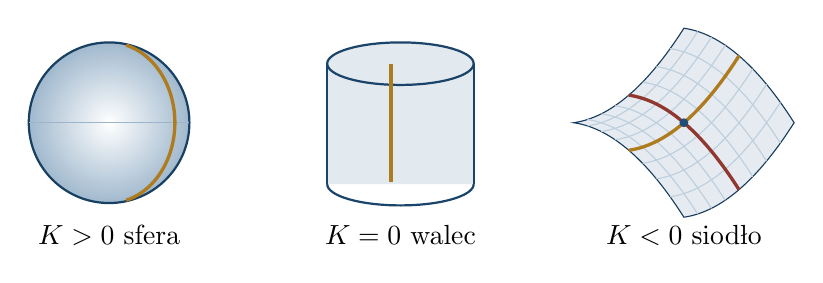
\begin{tikzpicture}[scale=1,>=Latex]
 \begin{scope}[shift={(-3.7,0)}]
  \shade[inner color=white,outer color=manifoldblue!43] (0,0) circle (1.02);
  \draw[manifoldblue!70!black,thick] (0,0) circle (1.02);
  \draw[manifoldblue!45] (-1.02,0)--(1.02,0);
  \draw[manifoldgold!85!black,very thick]
   plot[domain=15:165,samples=80] ({1.02*cos(35)*sin(\x)},{1.02*cos(\x)});
  \node at (0,-1.43) {$K>0$ sfera};
 \end{scope}
 \fill[manifoldblue!13] (-.93,-.78)--(.93,-.78)--(.93,.75)
  arc[start angle=0,end angle=180,x radius=.93,y radius=.27]--cycle;
 \draw[manifoldblue!75!black,thick]
  (-.93,-.78)--(-.93,.75) (.93,-.78)--(.93,.75);
 \draw[manifoldblue!75!black,thick] (0,.75) ellipse (.93 and .27);
 \draw[manifoldblue!75!black,thick] (-.93,-.78)
  arc[start angle=180,end angle=360,x radius=.93,y radius=.27];
 \draw[manifoldgold!85!black,very thick] (-.12,-.75)--(-.12,.74);
 \node at (0,-1.43) {$K=0$ walec};
 % Projection of (x,y,(x^2-y^2)/2) to (.7(x-y),.6(x+y)+.5z).
 \begin{scope}[shift={(3.6,0)}]
  \path[fill=manifoldblue!12,draw=manifoldblue!65!black]
   plot[domain=-1:1,samples=30] ({.7*(-1-\x)},{.6*(-1+\x)+.25*(1-(\x)^2)}) --
   plot[domain=-1:1,samples=30] ({.7*(\x-1)},{.6*(\x+1)+.25*((\x)^2-1)}) --
   plot[domain=1:-1,samples=30] ({.7*(1-\x)},{.6*(1+\x)+.25*(1-(\x)^2)}) --
   plot[domain=1:-1,samples=30] ({.7*(\x+1)},{.6*(\x-1)+.25*((\x)^2-1)}) -- cycle;
  \foreach \v in {-.75,-.5,-.25,0,.25,.5,.75} {
   \draw[manifoldblue!30,thin] plot[domain=-1:1,samples=30]
    ({.7*(\x-\v)},{.6*(\x+\v)+.25*((\x)^2-(\v)^2)});
   \draw[manifoldblue!30,thin] plot[domain=-1:1,samples=30]
    ({.7*(\v-\x)},{.6*(\v+\x)+.25*((\v)^2-(\x)^2)});
  }
  \draw[manifoldgold!85!black,very thick] plot[domain=-1:1,samples=50]
   ({.7*\x},{.6*\x+.25*(\x)^2});
  \draw[manifoldred!85!black,very thick] plot[domain=-1:1,samples=50]
   ({-.7*\x},{.6*\x-.25*(\x)^2});
  \fill[manifoldblue!85!black] (0,0) circle (1.6pt);
  \node at (0,-1.43) {$K<0$ siodło};
 \end{scope}
\end{tikzpicture}
\caption{Sfera ma dodatnią, walec zerową, a siodło ujemną krzywiznę Gaussa.
Złoty łuk na sferze jest rzutem łuku wielkiego okręgu. Na siodle
$z=(x^2-y^2)/2$ wyróżniono przekroje $y=0$ i $x=0$;
spotykają się w zaznaczonym punkcie, w którym $K=-1$.
Wartości $K$ wynikają z metryk tych powierzchni.}
\label{fig:krzywizna-znaki}
\end{figure}

\section{Ricci, krzywizna skalarna i przykłady modelowe}
\label{sec:ricci-krzywizna-skalarna}

\begin{definicja}[dwa ślady krzywizny]
\index{dwa slady krzywizny@dwa ślady krzywizny}
\label{def:ricci-skalarna}
\emph{Tensor Ricciego} jest śladem odwzorowania
$W\mapsto R(W,U)V$:
\begin{equation}\label{eq:ricci-def}
 \mathrm{Ric}(U,V)=\operatorname{tr}
              \bigl(W\longmapsto R(W,U)V\bigr),
 \qquad \mathrm{Ric}_{ij}=R^a{}_{j a i}.
\end{equation}
\emph{Krzywizna skalarna} to jeszcze jeden ślad,
tym razem względem metryki:
\begin{equation}\label{eq:scalar-def}
 \mathrm{Scal}=\operatorname{tr}_g\mathrm{Ric}
               =g^{ij}\mathrm{Ric}_{ij}.
\end{equation}
Nie mylmy $\mathrm{Scal}$ z operatorem $R$ ani
z wartością $K(\sigma)$ przypisaną płaszczyźnie.
\end{definicja}

Tensor Ricciego jest symetryczny. Istotnie, z pierwszej
tożsamości Bianchiego
$R(e_i,U)V-R(e_i,V)U=-R(U,V)e_i$.
Bierzemy iloczyn z $e_i$ i sumujemy po bazie ortonormalnej:
\[
 \mathrm{Ric}(U,V)-\mathrm{Ric}(V,U)
 =-\sum_i g(R(U,V)e_i,e_i)=0.
\]
Ostatnie składniki znikają przez antysymetrię w dwóch
ostatnich argumentach $\mathcal R$. W sygnaturze
pseudoriemannowskiej ta sama suma ma wagi
$\varepsilon_i=g(e_i,e_i)=\pm1$ i również znika.

Można to zobaczyć bez indeksów. Z punktu $p$ wysyłamy
geodezyjne w kierunku jednostkowego wektora $v$ i
w sąsiednich kierunkach. $\mathrm{Ric}(v,v)$ opisuje
\emph{łączny} wpływ krzywizn płaszczyzn rozpiętych
przez $v$ i każdy kierunek prostopadły na to, jak
rozszerza się wąska wiązka tych geodezyjnych.
Krzywizna skalarna zbiera te wyniki po wszystkich
kierunkach $v$. Ścisłe znaczenie słów ,,łącznie''
i ,,po wszystkich'' podają poniższe sumy.

\begin{stwierdzenie}[sumowanie krzywizn sekcyjnych]
\label{prop:ricci-sekcje}
Jeżeli $e_1,\ldots,e_n$ jest ortonormalną bazą
riemannowskiego $T_pM$, to
\begin{equation}\label{eq:ricci-suma-sekcji}
 \mathrm{Ric}(v,v)
 =\sum_{i=1}^n g(R(e_i,v)v,e_i).
\end{equation}
Dla jednostkowego $v=e_1$ jest to suma
$\sum_{i=2}^n K(\operatorname{span}\{e_1,e_i\})$.
Ponadto
\begin{equation}\label{eq:scalar-suma-sekcji}
 \mathrm{Scal}=2\sum_{1\leq i<j\leq n}
                    K(\operatorname{span}\{e_i,e_j\}).
\end{equation}
W wymiarze dwa: $\mathrm{Ric}=Kg$ oraz
$\mathrm{Scal}=2K$.
\end{stwierdzenie}

\begin{proof}
Ślad endomorfizmu w bazie ortonormalnej to suma
iloczynów skalarnych jego wartości na $e_i$ z $e_i$.
Stosując to do definicji~\eqref{eq:ricci-def},
dostajemy~\eqref{eq:ricci-suma-sekcji}. Składnik
z $e_i=v$ znika przez antysymetrię $R(v,v)=0$;
pozostałe są wartościami~\eqref{eq:krzywizna-sekcyjna}.
Ponowny ślad daje sumę po wszystkich parach
uporządkowanych $i\ne j$. Symetria par z
Twierdzenia~\ref{thm:symetrie-riemanna} sprawia,
że pary $(i,j)$ i $(j,i)$ mają tę samą krzywiznę;
stąd czynnik $2$. W wymiarze dwa dla jednostkowego
$v$ z pierwszej równości mamy
$\mathrm{Ric}(v,v)=K(p)$; jednorodność i polaryzacja
dają $\mathrm{Ric}=Kg$.
\end{proof}

\subsection*{Co mierzy Ricci, a co mierzy skalar?}
Załóżmy $n\geq2$. Ustalmy jednostkowy $v\in T_pM$ i patrzmy na geodezyjną
$\gamma_v(t)=\exp_p(tv)$. Sąsiednie promienie odchylone
w kierunkach prostopadłych do $v$ opisuje macierz pól
Jacobiego $A(t)$ z warunkami
$A(0)=0$, $A'(0)=\mathrm{Id}$; szczegóły konstrukcji
podamy w Sekcji~\ref{sec:druga-wariacja-jacobi}.
Ich równanie ma postać
$A''+\mathsf K_v(t)A=0$, gdzie
$\mathsf K_v(0)w=R(w,v)v$. Wstawiając warunki
początkowe i różniczkując równanie w zerze, otrzymujemy
\[
 A(t)=t\,\mathrm{Id}-\frac{t^3}{6}\mathsf K_v(0)+O(t^4).
\]
Dlaczego wyraz przy $t^2$ znika? Z równania
$A''(0)=-\mathsf K_v(0)A(0)=0$; trzecia pochodna
wynosi $A'''(0)=-\mathsf K_v(0)A'(0)=-\mathsf K_v(0)$.
Ślad $\mathsf K_v(0)$ to $\mathrm{Ric}(v,v)$, zatem
wyznacznik, czyli gęstość objętości w kierunku $v$,
spełnia
\begin{equation}\label{eq:ricci-gestosc-malej-kuli}
 j(t,v)=t^{n-1}\left(1-\frac{\mathrm{Ric}_p(v,v)}6t^2
                              +O(t^3)\right).
\end{equation}
Użyliśmy tu elementarnego rozwinięcia
$\det(\mathrm{Id}+\varepsilon B)
=1+\varepsilon\operatorname{tr}B+O(\varepsilon^2)$.
Przy dodatnim $\mathrm{Ric}(v,v)$ mała porcja objętości
wzdłuż tego promienia jest mniejsza niż w $\R^n$;
przy ujemnym jest większa. Mówimy o \emph{sumie}
odkształceń prostopadłych, nie o zachowaniu każdej
pojedynczej geodezyjnej.

Reszty są jednostajne względem $v\in S_pM$: zależność
rozwiązań od kierunku jest gładka, a sfera kierunków
jest zwarta. Dla dostatecznie małego $r$ kula metryczna
jest obrazem kuli stycznej przez $\exp_p$, zgodnie
z~\eqref{eq:male-kule-normalne}. Można zatem całkować
w tych współrzędnych bez wielokrotnego liczenia punktów.
Zsumujmy~\eqref{eq:ricci-gestosc-malej-kuli} po
wszystkich jednostkowych kierunkach. Symetria sfery
jednostkowej daje średnią
$\int_{S_pM}\mathrm{Ric}(v,v)\,\dd\theta/
\operatorname{area}(S^{n-1})=\mathrm{Scal}(p)/n$:
średnia $v_iv_j$ wynosi $\delta_{ij}/n$, a ślad
macierzy Ricciego to właśnie $\mathrm{Scal}$.
Całkując jeszcze promień $t$ od $0$ do $r$, przy
$b_n=\operatorname{vol}_{\R^n}(B_1(0))$ dostajemy
\begin{equation}\label{eq:scalar-mala-kula}
 \operatorname{vol}_g(B_g(p,r))
 =b_nr^n\left(1-\frac{\mathrm{Scal}(p)}{6(n+2)}r^2
                                      +O(r^3)\right).
\end{equation}
Faktycznie $\operatorname{area}(S^{n-1})=nb_n$,
a iloraz całek $\int_0^r t^{n+1}\dd t$ i
$\int_0^r t^{n-1}\dd t$ to $nr^2/(n+2)$.
Dodatnia krzywizna skalarna oznacza więc mniejszą
objętość bardzo małych kul niż w geometrii euklidesowej.
W wymiarze dwa $\mathrm{Scal}=2K$ i
\eqref{eq:scalar-mala-kula} daje
$\operatorname{Area}(B(p,r))
=\pi r^2(1-K(p)r^2/12+O(r^3))$, zgodnie z
obwodem~\eqref{eq:gauss-maly-okrag} po scałkowaniu.
Sam wzór na obwód otrzymujemy bez różniczkowania symbolu $O$:
dla $n=2$ całka gęstości $j(r,v)$ po $S_pM$ jest długością
okręgu geodezyjnego, więc
$C(r)=2\pi r(1-K(p)r^2/6+O(r^3))$.

Ślady tracą część danych: dodatnie i ujemne krzywizny
sekcyjne mogą się w nich znosić. W szczególności zerowy
$\mathrm{Ric}$ nie wymusza $R=0$ w wymiarze cztery.
W metrykach lorentzowskich przy śladzie występują też
znaki $\varepsilon_i=g(e_i,e_i)=\pm1$; powyższa
interpretacja objętości małych \emph{kul metrycznych}
dotyczy metryki riemannowskiej.

\begin{twierdzenie}[przestrzenie o stałej krzywiźnie]
\label{thm:stala-krzywizna}
Jeżeli wszystkie płaszczyzny styczne w rozmaitości
riemannowskiej wymiaru $n\geq2$ mają tę samą stałą
krzywiznę $\kappa$, to
\begin{equation}\label{eq:stala-krzywizna-tensor}
 R(X,Y)Z=\kappa\bigl(g(Y,Z)X-g(X,Z)Y\bigr),
 \quad \mathrm{Ric}=(n-1)\kappa g,
 \quad \mathrm{Scal}=n(n-1)\kappa.
\end{equation}
\end{twierdzenie}

\begin{proof}
Prawa strona wzoru na $R$ ma symetrie tensora
Riemanna i daje $K(\sigma)=\kappa$ dla każdej
płaszczyzny. Wykażmy, że te wartości wyznaczają
cały tensor. Niech $A$ będzie różnicą obu tensorów
z opuszczonym ostatnim indeksem. Ma ona symetrie
z Twierdzenia~\ref{thm:symetrie-riemanna} i
$A(u,v,v,u)=0$ dla wszystkich $u,v$.
Po podstawieniu $u+w$ w miejsce $u$ i użyciu
antysymetrii oraz symetrii zamiany par dostajemy
$A(u,v,v,w)=0$. Następnie podstawiamy $v+x$
w miejsce $v$: po odrzuceniu dwóch zerowych
wyrazów zostaje
\[
 A(u,v,x,w)+A(u,x,v,w)=0.
\]
Z antysymetrii w pierwszej parze wynika
$A(u,v,x,w)=A(x,u,v,w)$, a po cyklicznej
zamianie argumentów także
$A(u,v,x,w)=A(v,x,u,w)$. Pierwsza tożsamość
Bianchiego mówi, że suma tych trzech równych
wartości wynosi zero. Zatem $A=0$.
Ślad $W\mapsto R(W,U)V$ wzoru na $R$ jest
$\kappa(ng(U,V)-g(U,V))$, co daje $\mathrm{Ric}$.
Jeszcze jeden ślad daje $\mathrm{Scal}$.
\end{proof}

\begin{przyklad}[trzy geometrie modelowe]\label{prz:krzywizna-modele}
W $\R^n$ standardowe symbole Christoffela znikają:
$R=\mathrm{Ric}=\mathrm{Scal}=0$. Na sferze $S_a^n$
o promieniu $a$ w $\R^{n+1}$ operator kształtu
jest $S=\pm a^{-1}\mathrm{Id}$. Równanie Gaussa
\eqref{eq:gauss-rownanie}, ważne także dla
hiperpowierzchni, daje
$R(X,Y)Z=a^{-2}(g(Y,Z)X-g(X,Z)Y)$.
Zatem $K=a^{-2}$, $\mathrm{Ric}=(n-1)a^{-2}g$
i $\mathrm{Scal}=n(n-1)a^{-2}$.

Model hiperboloidy $\mathbb H^n=\{p:\langle p,p\rangle_L=-1,
p_0>0\}$ leży w płaskiej przestrzeni Minkowskiego.
Jej normalna $p$ ma kwadrat długości $-1$.
Z $Y\langle Z,p\rangle_L=0$ wynika
$\langle D_YZ,p\rangle_L=-g(Y,Z)$, a więc
$D_YZ=\nabla_YZ+g(Y,Z)p$. Ponadto $D_Xp=X$.
Biorąc część styczną komutatora płaskiej pochodnej
$D$ tak jak w dowodzie~\ref{thm:egregium}, uzyskujemy
\[
 R(X,Y)Z=-\bigl(g(Y,Z)X-g(X,Z)Y\bigr).
\]
Stąd $K=-1$, $\mathrm{Ric}=-(n-1)g$ i
$\mathrm{Scal}=-n(n-1)$. Po zmianie skali metryki
na $g_{\mathrm{nowe}}=a^2g$, $a>0$, otrzymujemy
$K=-a^{-2}$, $\mathrm{Ric}_{\mathrm{nowe}}
=-(n-1)a^{-2}g_{\mathrm{nowe}}=\mathrm{Ric}$ i
$\mathrm{Scal}_{\mathrm{nowe}}=-n(n-1)a^{-2}$.
Izometrie modeli z Przykładu~\ref{prz:trzy-modele-hiperboliczne}
przenoszą te wartości na model półprzestrzeni
i model kuli.
\end{przyklad}

\begin{stwierdzenie}[krzywizna w każdym z trzech modeli]
\label{prop:krzywizna-trzy-modele-hiperboliczne}
Metryki hiperboloidy, kuli Poincarégo
\eqref{eq:hip-kula} i półprzestrzeni
\eqref{eq:hip-polprzestrzen} mają tę samą
krzywiznę sekcyjną $K=-1$ w każdej płaszczyźnie.
W wymiarze $n$ w każdym modelu
$\mathrm{Ric}=-(n-1)g$ i
$\mathrm{Scal}=-n(n-1)$. Po pomnożeniu metryki
przez $a^2$ wartości te przyjmują odpowiednio
postać $K=-a^{-2}$,
$\mathrm{Ric}=-(n-1)a^{-2}g_{\mathrm{nowe}}$
oraz $\mathrm{Scal}=-n(n-1)a^{-2}$.
\end{stwierdzenie}

\begin{proof}
Dla hiperboloidy wynik otrzymaliśmy z płaskiej
pochodnej otaczającej w Przykładzie
\ref{prz:krzywizna-modele}. Odwzorowania
$P$ i $F$ z Przykładu
\ref{prz:trzy-modele-hiperboliczne} spełniają
$P^*g_{\mathcal H}=g_B$ oraz
$F^*g_{\mathbb H}=g_B$. Są zatem izometriami.
Jednoznaczność koneksji Leviego-Civity daje dla
izometrii $I$ równość
$\dd I(\nabla_XY)=\nabla_{\dd I X}(\dd I Y)$
(po odpowiednim przeniesieniu pól); wstawienie
jej do~\eqref{eq:riemann-def} przenosi tensor
$R$, a więc i~\eqref{eq:krzywizna-sekcyjna}.
To dowodzi tezy we wszystkich wymiarach.

Współrzędne $z$ pozwalają również sprawdzić
krzywiznę hiperboloidy \emph{bezpośrednio z symboli}.
Pisząc $t^2=1+|z|^2$, z
\eqref{eq:gamma-hiperboloida} mamy
\[
 \partial_i\Gamma^k_{j\ell}
   =-\delta_i^k g_{j\ell}-z^k\partial_i g_{j\ell},
 \qquad
 \Gamma^k_{ic}\Gamma^c_{j\ell}
   =\frac{z^k z_i}{t^2}g_{j\ell},
\]
ponieważ $z^c g_{ic}=z_i/t^2$. Z obliczonej
w rozdziale o koneksji pochodnej $g_{j\ell}$ wynika
\[
 \partial_i g_{j\ell}-\partial_j g_{i\ell}
    =\frac{\delta_{j\ell}z_i
                   -\delta_{i\ell}z_j}{t^2}.
\]
Po podstawieniu do~\eqref{eq:riemann-wspolrzedne}
wyrazy zawierające $z^k$ znoszą się. Zostaje
\begin{equation}\label{eq:riemann-hiperboloida-wspolrzedne}
 R^k{}_{\ell i j}
   =-\bigl(\delta_i^k g_{j\ell}
                        -\delta_j^k g_{i\ell}\bigr),
\end{equation}
co ponownie daje $K=-1$ dla każdej
płaszczyzny stycznej.

Policzmy dodatkowo krzywiznę \emph{wprost}
w wymiarze dwa. Dla metryki konforemnej
$g=e^{2\varphi}(\dd x^2+\dd y^2)$ wzór
\eqref{eq:christoffel-metryka} daje
\[
 \Gamma^k_{ij}
   =\delta_i^k\varphi_j+\delta_j^k\varphi_i
       -\delta_{ij}\varphi_k,
 \qquad \varphi_j=\partial_j\varphi.
\]
Przykładowo
$\Gamma^1_{11}=\varphi_x$,
$\Gamma^1_{12}=\varphi_y$,
$\Gamma^1_{22}=-\varphi_x$,
$\Gamma^2_{12}=\varphi_x$ i
$\Gamma^2_{22}=\varphi_y$.
W składniku $R^1{}_{2 1 2}$ wzoru
\eqref{eq:riemann-wspolrzedne} pochodne dają
$-\varphi_{xx}-\varphi_{yy}$, zaś dwa wyrazy
kwadratowe w symbolach Christoffela są
$(-\varphi_x^2+\varphi_y^2)$ i
$-(\varphi_y^2-\varphi_x^2)$, więc się znoszą.
Mianownik w~\eqref{eq:krzywizna-sekcyjna}
wynosi $e^{4\varphi}$, a licznik
$e^{2\varphi}R^1{}_{2 1 2}$; stąd
\begin{equation}\label{eq:gauss-konforemna}
 K=-e^{-2\varphi}\bigl(\varphi_{xx}
                                  +\varphi_{yy}\bigr).
\end{equation}
Dla półpłaszczyzny $\varphi=-\log y$:
$\Delta_{\mathrm E}\varphi=1/y^2$
i $e^{-2\varphi}=y^2$, co daje $K=-1$.
Dla dysku $r^2=x^2+y^2$ i
$\varphi=\log2-\log(1-r^2)$; obliczenie pochodnych
\[
 \varphi_x=\frac{2x}{1-r^2},\qquad
 \varphi_{xx}=\frac{2}{1-r^2}
                  +\frac{4x^2}{(1-r^2)^2}
\]
oraz analogiczne dla $y$ daje
$\Delta_{\mathrm E}\varphi=4/(1-r^2)^2$.
Ponieważ $e^{-2\varphi}=(1-r^2)^2/4$,
ponownie $K=-1$. Wzory na Ricciego i skalar
wynikają ze śladów w
\eqref{eq:stala-krzywizna-tensor}.

Przy skalowaniu $g\mapsto a^2g$ symbole
Christoffela pozostają takie same, więc operator
$R(X,Y)Z$ się nie zmienia. Licznik i mianownik
w~\eqref{eq:krzywizna-sekcyjna} mnożą się
odpowiednio przez $a^2$ i $a^4$; dlatego
$K\mapsto a^{-2}K$. Tensor Ricciego typu $(0,2)$
pozostaje niezmieniony: jego definicja bierze ślad
niezmienionego operatora $W\mapsto R(W,U)V$.
Dopiero ślad z nową odwrotnością metryki daje
$\mathrm{Scal}_{\mathrm{nowe}}=a^{-2}\mathrm{Scal}$.
Nie należy mylić niezmienionego tensora Ricciego
z jego wartościami na wektorach jednostkowych dla nowej metryki.
\end{proof}

\begin{przyklad}[różne płaszczyzny w jednym punkcie]
Na produkcie $S_a^2\times\R$ z metryką produktową
płaszczyzna styczna do sfery ma krzywiznę $a^{-2}$,
a płaszczyzna rozpięta przez kierunek sferyczny
i kierunek prostej ma krzywiznę $0$. W bazie
ortonormalnej złożonej z dwóch kierunków sfery
i jednego kierunku prostej tensor Ricciego ma
wartości diagonalne $(a^{-2},a^{-2},0)$,
zaś $\mathrm{Scal}=2a^{-2}$. Jedna liczba skalarna
nie mówi, która z płaszczyzn jest zakrzywiona.
\end{przyklad}

\begin{przyklad}[pomiar krzywizny obwodem koła]
\label{prz:obwod-kola-krzywizna}
Niech $\rho$ będzie \emph{odległością geodezyjną}
od ustalonego punktu na dwuwymiarowej przestrzeni
o stałej krzywiźnie. Współrzędne biegunowe na
sferze promienia $a$ dają
$g=\dd\rho^2+a^2\sin^2(\rho/a)\dd\phi^2$.
Na hiperboloidzie można zapisać punkt jako
$\bigl(a\cosh(\rho/a),
 a\sinh(\rho/a)\cos\phi,
 a\sinh(\rho/a)\sin\phi\bigr)$;
różniczkując tę parametryzację w metryce
Minkowskiego, dostajemy
$g=\dd\rho^2+a^2\sinh^2(\rho/a)\dd\phi^2$.
Na płaszczyźnie jest $g=\dd\rho^2+\rho^2\dd\phi^2$.
Okrąg $\rho=\mathrm{const}$ ma zatem obwód
$\int_0^{2\pi}\sqrt{g_{\phi\phi}}\,\dd\phi$, czyli
\begin{equation}\label{eq:obwod-kola-krzywizna}
 \begin{array}{c|c|c}
  \text{powierzchnia}& K & \text{obwód }C(\rho)\\ \hline
  S_a^2&+a^{-2}&2\pi a\sin(\rho/a),\quad 0<\rho<\pi a\\
  \R^2&0&2\pi\rho\\
  \mathbb H_a^2&-a^{-2}&2\pi a\sinh(\rho/a)
 \end{array}
\end{equation}
Ponieważ $\sin x=x-x^3/6+O(x^5)$ oraz
$\sinh x=x+x^3/6+O(x^5)$, mały okrąg na
sferze ma obwód \emph{mniejszy} od $2\pi\rho$,
a w przestrzeni hiperbolicznej \emph{większy}.
W każdym przypadku $C(\rho)=2\pi\rho
\bigl(1-K\rho^2/6+O(\rho^4)\bigr)$.
To sposób odczytania znaku krzywizny z pomiarów
wykonanych na samej powierzchni.
\end{przyklad}

\section{Schwarzschild i Kerr: próżnia nie oznacza płaskości}

W tej sekcji przyjmujemy jednostki $G=c=1$ i tę samą
konwencję znaku co w~\eqref{eq:riemann-def}. Metryki
\eqref{eq:schwarzschild} i~\eqref{eq:kerr} są
lorentzowskie. Ich $\mathrm{Ric}$ oraz $\mathrm{Scal}$
dotyczą \emph{pełnej czterowymiarowej czasoprzestrzeni};
metryki indukowane na przekrojach $t=\mathrm{const}$
mają własną, inną krzywiznę.

\begin{przyklad}[krzywizna metryki Schwarzschilda]
\label{prz:krzywizna-schwarzschild}
Dla $M>0$, w obszarze $r>2M$ i $0<\theta<\pi$, zapiszmy metrykę z
\eqref{eq:schwarzschild} jako
\[
 g=-f(r)\dd t^2+f(r)^{-1}\dd r^2
             +r^2\dd\theta^2+r^2\sin^2\theta\,\dd\phi^2,
 \qquad f(r)=1-\frac{2M}{r}.
\]
Aby zobaczyć, skąd biorą się wartości krzywizny,
podajmy obliczenie najpierw dla dowolnej gładkiej funkcji $f>0$.
Niezerowe symbole Christoffela, poza zamianą
dolnych indeksów, są następujące:
\begin{align*}
 \Gamma^t_{tr}&=\frac{f'}{2f},&
 \Gamma^r_{tt}&=\frac{ff'}2,&
 \Gamma^r_{rr}&=-\frac{f'}{2f},\\
 \Gamma^r_{\theta\theta}&=-rf,&
 \Gamma^r_{\phi\phi}&=-rf\sin^2\theta,&
 \Gamma^\theta_{r\theta}&=\Gamma^\phi_{r\phi}=\frac1r,\\
 \Gamma^\theta_{\phi\phi}&=-\sin\theta\cos\theta,&
 \Gamma^\phi_{\theta\phi}&=\cot\theta.
\end{align*}
Wstawienie ich do~\eqref{eq:riemann-wspolrzedne},
a następnie wykonanie śladu
$\mathrm{Ric}_{ij}=R^a{}_{j a i}$ daje
\begin{align}\label{eq:ricci-f-sferyczna}
 \mathrm{Ric}_{tt}&=f\left(\frac{f''}{2}+\frac{f'}r\right),
 &\mathrm{Ric}_{rr}&=-\frac1f
               \left(\frac{f''}{2}+\frac{f'}r\right),\notag\\
 \mathrm{Ric}_{\theta\theta}&=1-f-rf',
 &\mathrm{Ric}_{\phi\phi}&=(1-f-rf')\sin^2\theta,
\end{align}
zaś pozostałe składowe są zerowe. Dla kontroli
prześledźmy składową kątową. W ogólnym wzorze
\[
 \mathrm{Ric}_{ij}=\partial_a\Gamma^a_{ij}
   -\partial_j\Gamma^a_{ia}
   +\Gamma^a_{ac}\Gamma^c_{ij}
   -\Gamma^a_{jc}\Gamma^c_{ia}
\]
dla $i=j=\theta$ kolejne cztery grupy składników
wynoszą odpowiednio
\[
 -f-rf',\qquad \csc^2\theta,\qquad -2f,
 \qquad 2f-\cot^2\theta.
\]
Ich suma to $1-f-rf'$.
Teraz $f'=2M/r^2$ i $f''=-4M/r^3$:
zarówno $f''/2+f'/r$, jak i $1-f-rf'$ znikają.
Otrzymujemy
\begin{equation}\label{eq:schwarz-ricci-kretsch}
 \mathrm{Ric}=0,\qquad \mathrm{Scal}=0,
 \qquad \mathcal K:={\mathcal R}_{abcd}
                   {\mathcal R}^{abcd}=\frac{48M^2}{r^6}.
\end{equation}
Sprawdźmy również ostatnią równość, a przy okazji
wskażmy jawną składową niezerowego $R$.
Z~\eqref{eq:riemann-wspolrzedne} i podanych symboli
Christoffela znajdujemy między innymi
\[
 R^t{}_{rtr}=-\frac{f''}{2f},\qquad
 R^t{}_{\theta t\theta}=-\frac{rf'}2,\qquad
 R^r{}_{\theta r\theta}=-\frac{rf'}2,
\]
oraz, rozpisując składową kątową,
\[
 R^\theta{}_{\phi\theta\phi}
 =\partial_\theta\Gamma^\theta_{\phi\phi}
   +\Gamma^\theta_{\theta r}\Gamma^r_{\phi\phi}
   -\Gamma^\theta_{\phi\phi}
          \Gamma^\phi_{\theta\phi}
 =(1-f)\sin^2\theta.
\]
Składowe z $\phi$ w miejsce $\theta$ w parach
czasowo-kątowych i radialno-kątowych otrzymujemy
przez mnożenie przez $\sin^2\theta$. Weźmy
pseudoortonormalną ramkę o sygnaturze $(-,+,+,+)$
\[
 e_0=f^{-1/2}\partial_t,\quad
 e_1=f^{1/2}\partial_r,\quad
 e_2=r^{-1}\partial_\theta,\quad
 e_3=(r\sin\theta)^{-1}\partial_\phi
\]
i połóżmy $\mu=M/r^3$. Po obniżeniu indeksów
metryką i uwzględnieniu czynników w ramie
jedynymi niezależnymi niezerowymi wartościami są
\[
 \begin{array}{c|rrrrrr}
 (i,j)&(0,1)&(0,2)&(0,3)&(1,2)&(1,3)&(2,3)\\ \hline
 \mathcal R(e_i,e_j,e_j,e_i)
       &-2\mu&\mu&\mu&-\mu&-\mu&2\mu
 \end{array}
\]
Na przykład pierwsza wartość to $f''/2=-2\mu$,
druga to $f'/(2r)=\mu$, a ostatnia to
$(1-f)/r^2=2\mu$. Symetrie z
Twierdzenia~\ref{thm:symetrie-riemanna} dają
wszystkie pozostałe składowe; każda z sześciu
wartości występuje cztery razy przy pełnej
kontrakcji. Ponieważ w tych wyrazach indeks
czasowy występuje dwukrotnie,
\[
 \mathcal K=4\bigl((2\mu)^2+\mu^2+\mu^2
                     +\mu^2+\mu^2+(2\mu)^2\bigr)
           =48\mu^2=\frac{48M^2}{r^6}.
\]
Płaszczyzna $\operatorname{span}(\partial_\theta,
\partial_\phi)$ jest przestrzenna. W \emph{pełnej
czasoprzestrzeni} jej krzywizna sekcyjna wynosi
\begin{equation}\label{eq:schwarz-k-sekcyjna-katowa}
 K(\partial_\theta\wedge\partial_\phi)
 =\frac{r^2(1-f)\sin^2\theta}{r^4\sin^2\theta}
 =\frac{2M}{r^3}.
\end{equation}
Natomiast dwuwymiarowa sfera $t,r=\mathrm{const}$
z \emph{metryką indukowaną} ma krzywiznę Gaussa
$1/r^2$. Są to różne obiekty geometryczne;
nie wolno utożsamiać ich krzywizn. Niezmiennik
$\mathcal K$ z~\eqref{eq:schwarz-ricci-kretsch}
jest skończony przy $r=2M$, ale rośnie bez
ograniczenia, gdy $r\to0$ w przedłużeniu
czasoprzestrzeni. Zerowanie się Ricciego wynika
tu ze znoszenia się składowych śladu, a nie z
zaniku tensora Riemanna.
\end{przyklad}

\begin{przyklad}[krzywizna metryki Kerra]
\label{prz:krzywizna-kerr}
Niech $M>0$, $\Sigma=r^2+a^2\cos^2\theta$ i
$\Delta=r^2-2Mr+a^2$, jak we wzorze~\eqref{eq:kerr}.
Rachunek wykonamy dla $\Delta>0$, $\Sigma>0$ i
$0<\theta<\pi$. Wprowadźmy pseudoortonormalną ramkę
\[
 \begin{aligned}
 e_0&=\frac{(r^2+a^2)\partial_t+a\partial_\phi}
                  {\sqrt{\Sigma\Delta}},&
 e_1&=\sqrt{\frac\Delta\Sigma}\,\partial_r,\\
 e_2&=\frac{\partial_\theta}{\sqrt\Sigma},&
 e_3&=\frac{a\sin\theta\,\partial_t+
                      (\sin\theta)^{-1}\partial_\phi}{\sqrt\Sigma}.
 \end{aligned}
\]
Podstawienie do metryki daje $g(e_i,e_j)=
\operatorname{diag}(-1,1,1,1)_{ij}$. Poniższa tabela
pozwala sprawdzić oba ślady i pełną kontrakcję bez
pomijania składników mieszanych. Oznaczmy
\[
 A=\frac{Mr(r^2-3a^2\cos^2\theta)}{\Sigma^3},
 \qquad B=\frac{Ma\cos\theta(3r^2-a^2\cos^2\theta)}{\Sigma^3}.
\]
W kolejności par $01,02,03,12,13,23$ macierz
$C_{ij,kl}=\mathcal R(e_i,e_j,e_k,e_l)$ wynosi
\begin{equation}\label{eq:kerr-tabela-krzywizny}
 C=\begin{pmatrix}
 2A&0&0&0&0&-2B\\
 0&-A&0&0&-B&0\\
 0&0&-A&B&0&0\\
 0&0&B&A&0&0\\
 0&-B&0&0&A&0\\
 -2B&0&0&0&0&-2A
 \end{pmatrix}.
\end{equation}
Wszystkie inne składowe wyznaczają antysymetrie par.
Aby odtworzyć tabelę ze wzoru współrzędnego, wygodnie
położyć $x=\cos\theta$, $q=1-x^2$ i $\Sigma=r^2+a^2x^2$.
W kolejności $(t,r,x,\phi)$ niezerowe składowe odwrotnej
metryki są
\[
 \begin{aligned}
 g^{tt}&=-\frac{(r^2+a^2)^2-a^2\Delta q}{\Sigma\Delta},
 &g^{t\phi}&=-\frac{2Mar}{\Sigma\Delta},\\
 g^{\phi\phi}&=\frac{\Delta-a^2q}{\Sigma\Delta q},
 &g^{rr}&=\frac\Delta\Sigma,\qquad g^{xx}=\frac q\Sigma.
 \end{aligned}
\]
Współczynniki są wymierne w $r,x$; pochodne po $t,\phi$
znikają. Wstawiamy je do~\eqref{eq:christoffel-metryka}
i~\eqref{eq:riemann-wspolrzedne}, opuszczamy indeks metryką
i przechodzimy do powyższej ramki. Na przykład dla
$F_0=(r^2+a^2)\partial_t+a\partial_\phi$,
$F_1=\partial_r$, $F_2=-\partial_x$,
$F_3=aq\partial_t+\partial_\phi$ otrzymujemy
\[
 \begin{split}
 \mathcal R(F_0,F_1,F_0,F_1)&=
                  \frac{2Mr(r^2-3a^2x^2)}\Sigma,\\
 \mathcal R(F_0,F_1,F_2,F_3)&=
                 -\frac{2Max(3r^2-a^2x^2)}\Sigma.
 \end{split}
\]
Iloczyny czynników normalizujących w obu tych
składowych wynoszą $\Sigma^{-2}$, co daje $2A$ i $-2B$.
Pozostałe pary oblicza się tą samą skończoną procedurą.

Teraz $\mathrm{Ric}_{00}=-2A+A+A=0$,
$\mathrm{Ric}_{11}=2A-A-A=0$, a
$\mathrm{Ric}_{22}=\mathrm{Ric}_{33}=-A-A+2A=0$.
Składowe $B$ mają cztery różne indeksy, więc nie wnoszą
nic do śladu; pozadiagonalne składowe Ricciego też znikają.
Stąd $\mathrm{Ric}=0$ i $\mathrm{Scal}=0$.
Przy pełnej kontrakcji każda pozycja diagonalna tabeli
występuje cztery razy, a każda niezależna pozycja
pozadiagonalna osiem razy. Wyrazy $B$ mają jeden indeks
czasowy i wnoszą znak ujemny. Zatem
\[
 \mathcal K=4(4+1+1+1+1+4)A^2-8(4+1+1)B^2
           =48(A^2-B^2).
\]
Rozwinięcie
$r^2(r^2-3y^2)^2-y^2(3r^2-y^2)^2
=r^6-15r^4y^2+15r^2y^4-y^6$, dla $y=a\cos\theta$,
daje
\begin{equation}\label{eq:kerr-kretschmann}
 \mathcal K
 =\frac{48M^2}{\Sigma^6}
 \bigl(r^6-15a^2r^4\cos^2\theta
       +15a^4r^2\cos^4\theta-a^6\cos^6\theta\bigr).
\end{equation}
Można sprawdzić dwa ważne przypadki bez ponawiania
całego rachunku: dla $a=0$ odzyskujemy
$48M^2/r^6$ z~\eqref{eq:schwarz-ricci-kretsch},
a na równiku $\theta=\pi/2$ mamy tę samą wartość
nawet przy $a\ne0$. Poza równikiem pojawia się
zależność kątowa związana z obrotem. W sygnaturze
lorentzowskiej pełna kontrakcja $\mathcal K$ nie jest
kwadratem dodatniej normy: może mieć różne znaki.
Współrzędny rachunek krzywizny jest wymierny w $r,x$;
otrzymane tożsamości po sprowadzeniu do wspólnego mianownika
są tożsamościami wielomianowymi. Obowiązują więc również
na pozostałych obszarach $\Delta\ne0$, $\Sigma>0$,
choć użyta ramka z pierwiastkiem $\Delta$ nie jest tam rzeczywista.
Równanie $\Sigma=0$ dla $a\ne0$ odpowiada
$r=0,\theta=\pi/2$ i wskazuje osobliwość
pierścieniową: wzdłuż równika $\mathcal K=48M^2/r^6$
rośnie bez ograniczenia. Usuwalność osobliwości współrzędnych
przy $\Delta=0$, $\Sigma>0$, uzasadnia inny rachunek,
nie sama skończoność $\mathcal K$. Wprowadzamy lokalnie
\[
 \dd v=\dd t+\frac{r^2+a^2}{\Delta}\dd r,
 \qquad \dd\psi=\dd\phi+\frac a\Delta\dd r.
\]
Po podstawieniu do metryki wszystkie mianowniki $\Delta$
znoszą się i otrzymujemy
\[
 \begin{split}
 g={}&-\left(1-\frac{2Mr}{\Sigma}\right)\dd v^2
       +2\dd v\dd r-\frac{4Mar\sin^2\theta}{\Sigma}\dd v\dd\psi
       -2a\sin^2\theta\,\dd r\dd\psi\\
    &+\Sigma\dd\theta^2
       +\sin^2\theta\left(r^2+a^2+
                 \frac{2Mra^2\sin^2\theta}{\Sigma}\right)\dd\psi^2.
 \end{split}
\]
Jej wyznacznik wynosi $-\Sigma^2\sin^2\theta$.
Zatem dla $0<\theta<\pi$ i $\Sigma>0$ nowy wzór jest
gładki i niezdegenerowany także przy $\Delta=0$.
Definiuje lokalne przedłużenie przez tę powierzchnię.
Te stwierdzenia dotyczą pełnej
metryki lorentzowskiej. Przekrój $t=\mathrm{const}$
może mieć niezerowy tensor Ricciego własnej
metryki trójwymiarowej.
\end{przyklad}

\begin{uwaga}[interpretacja porównawcza]
Na sferze już Ricci i skalar rejestrują dodatnią
krzywiznę. W próżniowych przykładach Schwarzschilda
i Kerra oba te ślady znikają, choć transport po
pętlach i zachowanie sąsiednich geodezyjnych ujawniają
niezerowy tensor $R$. W czterowymiarowej geometrii
lorentzowskiej pozostaje wtedy część krzywizny,
która nie jest opisana przez Ricciego (tensor Weyla).
Pełny rozkład na część bezśladową i składniki
wyznaczone przez Ricciego wykracza poza ten rozdział.
\end{uwaga}

\section{Kiedy metryka jest naprawdę płaska?}

\begin{twierdzenie}[lokalna charakteryzacja płaskości]
\label{thm:lokalna-plaskosc}
Niech $(M,g)$ będzie rozmaitością riemannowską
i $p\in M$. Następujące warunki są równoważne
w odpowiednio małym otoczeniu $p$:
\begin{enumerate}[label=\textup{(\roman*)}]
 \item tensor Riemanna znika: $R\equiv0$;
 \item transport równoległy jest lokalnie niezależny
       od drogi o ustalonych końcach;
 \item istnieje ortonormalna rama pól równoległych
       $E_1,\ldots,E_n$;
 \item istnieją współrzędne $(x^1,\ldots,x^n)$,
       w których $g=\sum_i(\dd x^i)^2$;
 \item otoczenie $p$ jest izometryczne z otwartym
       podzbiorem $\R^n$.
\end{enumerate}
Ponadto $R=0$ wtedy i tylko wtedy, gdy
$K_p(\sigma)=0$ dla każdej płaszczyzny stycznej
we wszystkich punktach tego otoczenia.
W przypadku pseudoriemannowskim równoważność
warunków \textup{(i)--(iii)} i wersji \textup{(iv)}
z metryką stałą właściwej sygnatury jest taka sama.
\end{twierdzenie}

\begin{proof}
Wybierzmy małą, ściągalną kulę współrzędnych $U$
wokół $p$. Załóżmy (i). Pokażemy dokładnie,
dlaczego transport po różnych drogach daje to samo.
Niech $H(s,t)$ będzie gładką homotopią dróg
od $p$ do ustalonego $q\in U$, z nieruchomymi
końcami, $0\leq s,t\leq1$. Przenieśmy
$v\in T_pM$ równolegle wzdłuż każdej drogi
$t\mapsto H(s,t)$; oznaczmy otrzymane pole
wzdłuż $H$ przez $V(s,t)$. Mamy $\nabla_tV=0$.
Także gdy $H$ nie jest immersją, pochodne pól wzdłuż
$H$ spełniają regułę komutacji. Współrzędnie mają
postać $D_\alpha=\partial_\alpha+A_\alpha$, gdzie
$A_\alpha=\Gamma_i(H)\partial_\alpha H^i$.
Rozwinięcie komutatora daje
$[D_t,D_s]=\partial_tA_s-\partial_sA_t+[A_t,A_s]
=R(\partial_tH,\partial_sH)$: mieszane drugie pochodne
$H$ znoszą się, a pozostałe składniki są dokładnie
wzorem~\eqref{eq:riemann-wspolrzedne}. Stąd
\[
 \nabla_t(\nabla_sV)
 =\nabla_s(\nabla_tV)+R(\partial_tH,\partial_sH)V=0.
\]
Na początku $V(s,0)=v$, stąd $\nabla_sV(s,0)=0$.
Jednoznaczność równania transportu równoległego
wzdłuż $t$ daje $\nabla_sV(s,t)=0$ dla każdego
$t$, zwłaszcza przy $t=1$. Transport jest więc
niezależny od homotopii z ustalonymi końcami.
W wypukłym obrazie kuli współrzędnych dwie drogi
łączymy homotopią liniową
$H(s,t)=x^{-1}((1-s)x(\gamma_0(t))+s x(\gamma_1(t)))$.
Zachowuje ona końce. Dla dróg odcinkami gładkich
wybieramy wspólny skończony podział parametru $t$;
powyższy rachunek stosujemy kolejno na jego przedziałach.
Na łączeniach wartości $V$ i $\nabla_sV$ są zgodne,
więc argument przechodzi przez cały podział. Dowodzi to (ii).

Wybierzmy ortonormalną bazę $e_1,\ldots,e_n$ w $T_pM$
i przenieśmy każdy $e_i$ do $q\in U$. Niezależność
od drogi definiuje pole $E_i(q)$; transport po
radialnych drogach zależy gładko od końca,
więc $E_i$ są gładkie. Idąc najpierw do $q$,
a potem po dowolnej krótkiej krzywej przez $q$,
widzimy $\nabla_XE_i=0$ dla wszystkich $X$.
Zgodność koneksji z metryką zachowuje iloczyny
skalarne: $g(E_i,E_j)=\delta_{ij}$ na $U$.
Otrzymaliśmy (iii).

Koneksja Leviego-Civity nie ma torsji, więc
\[
 [E_i,E_j]=\nabla_{E_i}E_j-\nabla_{E_j}E_i=0.
\]
Przepływy komutujących pól komutują lokalnie.
Odwzorowanie otrzymane przez wykonanie po kolei
ich przepływów z czasami $x^1,\ldots,x^n$,
zaczynając od $p$, jest lokalnym dyfeomorfizmem
(jego różniczka w zerze wysyła bazę standardową
na $E_i(p)$). Komutowanie przepływów sprawia,
że w powstałych współrzędnych $E_i=\partial_i$.
Stąd $g_{ij}=g(E_i,E_j)=\delta_{ij}$, czyli (iv).
Odwzorowanie współrzędnych jest wtedy izometrią
na otwarty podzbiór $\R^n$, więc (iv) daje (v).
Izometria zachowuje koneksję i $R$, a w $\R^n$
standardowa koneksja ma $R=0$: (v) daje (i).
Implikacje (iii)$\Rightarrow$(ii) można też
sprawdzić bezpośrednio: współczynniki wektora
w ramie równoległej nie zmieniają się podczas
transportu.

Jeśli $R=0$, wzór~\eqref{eq:krzywizna-sekcyjna}
daje $K=0$. Odwrotność jest dokładnie krokiem
polaryzacji w dowodzie Twierdzenia
\ref{thm:stala-krzywizna} dla $\kappa=0$.
W sygnaturze pseudoriemannowskiej wybieramy
bazę ortonormalną z $g(e_i,e_i)=\pm1$; reszta
dowodu pozostaje bez zmian, a metryka w
współrzędnych ma stałe współczynniki $\pm1$.
\end{proof}

\begin{wniosek}[niski wymiar a płaskość]
\label{cor:ricci-plaskosc-3d}
Na powierzchni riemannowskiej $\mathrm{Scal}=0$
w otoczeniu wtedy i tylko wtedy, gdy metryka jest
tam lokalnie płaska. W wymiarze trzy wystarcza
$\mathrm{Ric}=0$ w otoczeniu. W wymiarze cztery
dla metryk lorentzowskich $\mathrm{Ric}=0$
nie wymusza już płaskości.
\end{wniosek}
\begin{proof}
W wymiarze dwa $\mathrm{Scal}=2K$ na mocy
Stwierdzenia~\ref{prop:ricci-sekcje}; stosujemy
Twierdzenie~\ref{thm:lokalna-plaskosc}.
W wymiarze trzy i przy $\mathrm{Ric}=0$ wybierzmy
\emph{dowolną} bazę ortonormalną $e_1,e_2,e_3$.
Oznaczając $K_{ij}=K(e_i\wedge e_j)$, dostajemy
z~\eqref{eq:ricci-suma-sekcji}
\[
 K_{12}+K_{13}=0,\qquad
 K_{12}+K_{23}=0,\qquad
 K_{13}+K_{23}=0.
\]
Po odjęciu dwóch pierwszych równań mamy
$K_{13}=K_{23}$; trzecie wymusza
$K_{13}=K_{23}=0$, a pierwsze daje $K_{12}=0$.
Każda płaszczyzna w $T_pM$ może być pierwszą
płaszczyzną pewnej bazy ortonormalnej; skoro
baza była dowolna, wszystkie krzywizny sekcyjne
znikają. Twierdzenie~\ref{thm:lokalna-plaskosc}
daje płaskość. Odwrotne implikacje są oczywiste,
bo $R=0$ pociąga oba zerowe ślady.
Kontrprzykłady w wymiarze cztery dają
\eqref{eq:schwarz-ricci-kretsch} i
\eqref{eq:kerr-kretschmann}: są lorentzowskie
i mają $\mathrm{Ric}=0$ przy $R\ne0$.
\end{proof}

\begin{uwaga}[lokalnie a globalnie]
Twierdzenie jest lokalne. Płaski torus
$\R^2/\mathbb Z^2$ ma $R=0$ i lokalnie wygląda
jak płaszczyzna, lecz globalnie ma inną topologię
i nie jest izometryczny z całą $\R^2$.
Walec z Przykładu~\ref{prz:egregium-cztery}
również jest lokalnie płaski. Sama równość
$\mathrm{Scal}=0$ jest znacznie słabsza od
$R=0$, co pokazują przykłady Schwarzschilda
i Kerra.
\end{uwaga}

\section{Holonomia: transport po wszystkich pętlach}
\label{sec:holonomia}
\index{holonomia}

W Uwadze~\ref{uwaga:holonomia} jedna mała pętla wykrywała
krzywiznę w punkcie. Teraz ustalimy punkt $p$ i zbierzemy
transporty po \emph{wszystkich} pętlach zaczynających się w $p$.
W ten sposób lokalny pomiar krzywizny łączy się z globalną
budową metryki. W całej sekcji $(M,g)$ jest spójną rozmaitością
riemannowską bez brzegu, a $P_\gamma$ oznacza transport
Leviego-Civity z Twierdzenia~\ref{thm:transport-rownolegly}.

\begin{definicja}[Pełna i ograniczona grupa holonomii]
\label{def:grupa-holonomii}
\index{holonomia!pełna}
\index{holonomia!ograniczona}
\emph{Grupą holonomii} w $p$ nazywamy
\[
 \operatorname{Hol}_p(M,g)
 =\{P_\gamma:T_pM\longrightarrow T_pM:\
   \gamma\text{ jest pętlą odcinkami gładką z bazą }p\}.
\]
Jej podzbiór otrzymany tylko z pętli ściągalnych
z zachowaniem punktu bazowego oznaczamy przez
$\operatorname{Hol}^0_p(M,g)$ i nazywamy
\emph{holonomią ograniczoną}. Transport po pętli jest
izometrią $T_pM$, więc obie grupy działają na tej samej
euklidesowej przestrzeni stycznej. Nazwa ``ograniczona''
dotyczy rodzaju pętli, a nie ograniczenia długości pętli.
\end{definicja}

Intuicja jest następująca: dwa sposoby przeniesienia wektora
z $p$ do $q$ mogą dać różne wyniki. Po powrocie z $q$ do $p$
ich różnica staje się elementem holonomii. Na płaszczyźnie
euklidesowej nie ma takiej różnicy; na sferze może ona być
obrotem, jak na Rysunku~\ref{fig:krzywizna-holonomia}.

\begin{figure}[htbp]
\centering
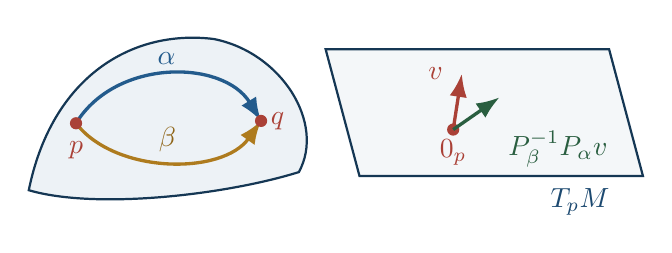
\begin{tikzpicture}[>=Latex,scale=1]
  \fill[manifoldblue!8] (-3.05,-.95)
    .. controls (-2.2,-1.20) and (-.55,-1.01) .. (.38,-.72)
    .. controls (.72,-.10) and (.16,.80) .. (-.70,.97)
    .. controls (-1.75,1.10) and (-2.76,.48) .. cycle;
  \draw[manifoldblue!60!black,thick] (-3.05,-.95)
    .. controls (-2.2,-1.20) and (-.55,-1.01) .. (.38,-.72)
    .. controls (.72,-.10) and (.16,.80) .. (-.70,.97)
    .. controls (-1.75,1.10) and (-2.76,.48) .. cycle;
  \coordinate (hp) at (-2.45,-.10);
  \coordinate (hq) at (-.10,-.07);
  \draw[manifoldblue,very thick,->] (hp)
    .. controls (-1.94,.73) and (-.58,.71) .. (hq);
  \draw[manifoldgold!85!black,very thick,->] (hp)
    .. controls (-1.95,-.75) and (-.59,-.76) .. (hq);
  \fill[manifoldred] (hp) circle (2.2pt) node[below=3pt] {$p$};
  \fill[manifoldred] (hq) circle (2.2pt) node[right] {$q$};
  \node[manifoldblue] at (-1.30,.72) {$\alpha$};
  \node[manifoldgold!70!black] at (-1.29,-.31) {$\beta$};
  \draw[manifoldblue!60!black,thick,fill=manifoldblue!5]
    (1.15,-.77)--(4.75,-.77)--(4.32,.84)--(.72,.84)--cycle;
  \fill[manifoldred] (2.34,-.18) circle (2.2pt) node[below] {$0_p$};
  \draw[manifoldred,very thick,->] (2.34,-.18)--++(.11,.71)
    node[left=3pt] {$v$};
  \draw[manifoldgreen!75!black,very thick,->]
    (2.34,-.18)--++(.59,.41);
  \node[manifoldgreen!75!black] at (3.67,-.43)
    {$P_\beta^{-1}P_\alpha v$};
  \node[manifoldblue!80!black] at (3.95,-1.10) {$T_pM$};
\end{tikzpicture}
\caption{Dwie drogi z $p$ do $q$. Po przejściu $\alpha$
i powrocie wzdłuż $\beta$ wynik w $T_pM$ wynosi
$P_\beta^{-1}P_\alpha v$; rysunek nie wyznacza wielkości
obrotu ani kąta między drogami.}
\label{fig:holonomia-dwie-drogi}
\end{figure}

\begin{stwierdzenie}[Działanie pętli i zmiana punktu bazowego]
\label{prop:holonomia-grupa-baza}
Zbiory z Definicji~\ref{def:grupa-holonomii} są podgrupami
$O(T_pM)$, a $\operatorname{Hol}^0_p$ jest podgrupą
normalną $\operatorname{Hol}_p$. Jeśli $\alpha$ prowadzi
z $p$ do $q$, to
\begin{equation}\label{eq:holonomia-zmiana-bazy}
 \operatorname{Hol}_q=P_\alpha\operatorname{Hol}_pP_\alpha^{-1}.
\end{equation}
Gdy $M$ jest jednospójna, $\operatorname{Hol}^0_p=
\operatorname{Hol}_p$.
\end{stwierdzenie}
\begin{proof}
Stała pętla daje identyczność. Jeśli najpierw idziemy po
$\gamma$, a potem po $\delta$, jednoznaczność równania
transportu daje $P_{\gamma\text{ potem }\delta}
=P_\delta P_\gamma$. Przejście pętli w przeciwnym kierunku
rozwiązuje to samo równanie od końca, więc
$P_{\gamma^{-1}}=P_\gamma^{-1}$. Pokazuje to domknięcie
na iloczyny i odwrotności. Zgodność koneksji z metryką
daje $g_p(P_\gamma v,P_\gamma w)=g_p(v,w)$, a więc
$P_\gamma\in O(T_pM)$.

Sklejenie pętli ściągalnych i odwrócenie jednej z nich
zachowuje ściągalność. Sprzężenie pętli ściągalnej
dowolną pętlą także jest ściągalne: najpierw wykonujemy
drogę sprzęgającą, następnie skurcz środkowej pętli,
a na końcu wracamy po drodze odwrotnej. To dowodzi
normalności. Każda pętla przy $q$ po dodaniu na początku
$\alpha$ i na końcu $\alpha^{-1}$ staje się pętlą
przy $p$. Rozpisanie transportów i odwrócenie tej
operacji daje~\eqref{eq:holonomia-zmiana-bazy}.
Na rozmaitości jednospójnej każda pętla jest ściągalna.
\end{proof}

Sama homotopijność dwóch pętli \emph{nie} oznacza, że
mają identyczny transport: na sferze nawet pętle
ściągalne mogą obracać wektor. W płaskiej geometrii
ograniczona holonomia znika i wtedy topologia może
pozostać jedynym źródłem niezerowej holonomii.

\begin{stwierdzenie}[Płaskość a holonomia ograniczona]
\label{prop:holonomia-plaskosc}
Dla spójnej rozmaitości riemannowskiej
\[
 R\equiv0\quad\Longleftrightarrow\quad
 \operatorname{Hol}^0_p=\{\operatorname{id}_{T_pM}\}.
\]
\end{stwierdzenie}
\begin{proof}
Jeżeli $R=0$, weźmy homotopię $H(s,t)$ pętli $\gamma$
do pętli stałej, z nieruchomym punktem bazowym.
Przenieśmy $v$ równolegle wzdłuż każdej krzywej
$t\mapsto H(s,t)$, otrzymując $V(s,t)$.
Rachunek komutatora pochodnych kowariantnych
z dowodu Twierdzenia~\ref{thm:lokalna-plaskosc} daje
$\nabla_t\nabla_sV=R(\partial_tH,\partial_sH)V=0$.
Na początku $\nabla_sV(s,0)=0$, więc przez jednoznaczność
transportu $\nabla_sV(s,1)=0$. Wynik transportu nie
zmienia się podczas homotopii i przy pętli stałej
wynosi $v$. Rachunek stosuje się na skończonym podziale
parametrów, gdy homotopia jest tylko odcinkami gładka.

Odwrotnie każda mała pętla z Uwagi~\ref{uwaga:holonomia}
jest ściągalna. Przy trywialnej holonomii ograniczonej
jej transport jest identycznością. Dla dowolnych
$X,Y,v\in T_qM$ wzór tamże daje
$0=-\varepsilon^2R_q(X,Y)v+O(\varepsilon^3)$.
Po podzieleniu przez $\varepsilon^2$ i przejściu
do granicy mamy $R_q(X,Y)v=0$. Punkt $q$ był dowolny:
trywialność w $p$ przenosi się na $q$ przez
sprzężenie~\eqref{eq:holonomia-zmiana-bazy}, także
dla pętli ściągalnych. Zatem $R\equiv0$.
\end{proof}

\begin{przyklad}[Płaski torus i płaska butelka Kleina]
\label{prz:holonomia-torus-klein}
Na $T^2=\R^2/\Z^2$ standardowe pola $\partial_x,\partial_y$
schodzą do globalnej ramy równoległej. Transport zachowuje
ich współczynniki, więc $\operatorname{Hol}_p(T^2)=\{1\}$,
choć torus nie jest jednospójny.

Inaczej jest dla płaskiej butelki Kleina
\[
 K=\R^2/\langle a,b\rangle,
 \qquad a(x,y)=(x+1,y),\qquad b(x,y)=(-x,y+1).
\]
Te izometrie generują swobodne, dyskretne działanie;
prostokąt podstawowy po sklejeniu boków daje zwartą
rozmaitość. Pętla w $K$ podnosi się do drogi w $\R^2$
od $\widetilde p$ do $h\widetilde p$ dla pewnego
przekształcenia $h$ z tej grupy. W $\R^2$ transport
zachowuje współrzędne wektora, a identyfikacja przestrzeni
stycznych na końcu używa $D h^{-1}$. Ponieważ
$Da=I$ i $Db=\operatorname{diag}(-1,1)$, dostajemy
\[
 \operatorname{Hol}_p(K)
   =\{I,\operatorname{diag}(-1,1)\},
 \qquad \operatorname{Hol}^0_p(K)=\{I\}.
\]
Obie metryki są lokalnie płaskie. Butelka pokazuje,
że $R=0$ nie wymusza trywialności \emph{pełnej}
holonomii.
\end{przyklad}

\begin{przyklad}[Holonomia okrągłej sfery]
\label{prz:holonomia-sfera}
Na zorientowanej $S_R^2$ transport zachowuje orientację:
jego wyznacznik zmienia się ciągle wzdłuż drogi,
a na początku wynosi $1$. Zatem
$\operatorname{Hol}_p(S_R^2)\subset SO(T_pS_R^2)$.
W Przykładzie~\ref{prz:transport-sfera} obliczyliśmy,
że obieg równoleżnika o kącie biegunowym $\theta$ daje obrót
o $-2\pi\cos\theta$ modulo $2\pi$. Aby przenieść tę
pętlę do ustalonego punktu $p$, dochodzimy z $p$ do
równoleżnika, wykonujemy obieg i wracamy tą samą drogą.
Otrzymany obrót jest sprzężony z poprzednim przez
izometrię zachowującą orientację. W $SO(2)$ takie
sprzężenie nie zmienia kąta. Gdy $0<\theta<\pi$,
wartości $-2\pi\cos\theta$ modulo $2\pi$ obejmują
wszystkie kąty. Stąd
$\operatorname{Hol}_p(S_R^2)=SO(T_pS_R^2)$.
Sfera jest jednospójna, więc jest to także jej
holonomia ograniczona. Nie ma na niej niezerowego
globalnego pola równoległego.
\end{przyklad}

\begin{uwaga}[Krzywizna wytwarza holonomię]
\label{uwaga:ambrose-singer-holonomia}
Wzór z Uwagi~\ref{uwaga:holonomia} pokazuje, że
$R_p(X,Y)$ jest kierunkiem nieskończenie małych
transportów po pętlach ściągalnych. Dokładną wersją
jest \emph{twierdzenie Ambrose'a--Singera}:
algebra Liego grupy $\operatorname{Hol}^0_p$ jest
rozpięta nad $\R$ przez operatory
\[
 P_\gamma^{-1}R_q(u,v)P_\gamma,
 \qquad \gamma:p\longrightarrow q,\quad
 u,v\in T_qM.
\]
Algebra Liego, wprowadzona w Sekcji~\ref{sec:algebra-liego},
to tutaj przestrzeń kierunków stycznych do grupy
w identyczności; fakt, że holonomia ograniczona ma
strukturę grupy Liego, także należy do cytowanego
wyniku o holonomii. Jedno zawieranie sugeruje rachunek małej
pętli; odwrotne jest głęboką częścią twierdzenia, której
nie dowodzimy. Źródłem jest
\href{https://doi.org/10.1090/S0002-9947-1953-0063739-1}
{W.~Ambrose i I.~M.~Singer, \emph{A theorem on holonomy},
Trans. Amer. Math. Soc. 75 (1953), 428--443}.
\end{uwaga}

\section{Niezmienniki holonomii i rozkład de Rhama}
\label{sec:rozklad-de-rhama}
\index{rozkład de Rhama}

Twierdzenie de Rhama z Rozdziału~\ref{ch:formy-de-rham}
porównuje kohomologię form z kohomologią singularną.
\emph{Twierdzenie o rozkładzie de Rhama} jest innym
wynikiem: rozpoznaje w metryce iloczyn czynników na
podstawie transportu równoległego. Najpierw udowodnimy
część lokalną i zobaczymy dokładnie, gdzie zaczyna się
krok globalny.

\begin{stwierdzenie}[Zasada holonomii dla pól równoległych]
\label{prop:zasada-holonomii}
Niech $E$ będzie wiązką tensorową nad spójną $M$,
z koneksją indukowaną przez $\nabla$. Wartość w $p$
zadaje bijekcję
\[
 \{s\in\Gamma(E):\nabla s=0\}
 \longleftrightarrow (E_p)^{\operatorname{Hol}_p},
\]
gdzie po prawej stoją elementy zachowywane przez
transport po wszystkich pętlach w $p$.
\end{stwierdzenie}
\begin{proof}
Jeśli $s$ jest równoległy, ograniczenie $s$ do każdej
krzywej rozwiązuje równanie transportu. Dla pętli
$\gamma$ przy $p$ mamy więc $P_\gamma s(p)=s(p)$.

Odwrotnie wybierzmy $a\in E_p$ stały pod całą
holonomią i połóżmy $s(q)=P_\alpha a$, gdzie
$\alpha$ prowadzi z $p$ do $q$. Jeśli $\beta$ jest
drugą taką drogą, to $P_\beta^{-1}P_\alpha$
jest transportem po pętli przy $p$. Z niezmienniczości
$a$ wynika $P_\alpha a=P_\beta a$; definicja jest
niezależna od drogi. W małym otoczeniu $q_0$ możemy
dołączyć do ustalonej drogi $p\to q_0$ krótkie odcinki
promieniowe zależne gładko od końca. Gładka zależność
rozwiązań równania transportu od parametrów dowodzi,
że $s$ jest gładki. Dla każdej krzywej $c:q\to r$
dołączamy $c$ do drogi $p\to q$ i dostajemy
$P_c s(q)=s(r)$. Zatem $s$ jest równoległy.
Obie konstrukcje są wzajemnie odwrotne.
\end{proof}

W szczególności podprzestrzeń niezmienniczą przez holonomię
$W\subset T_pM$ można przenosić do innych punktów:
$\mathcal E_q=P_\alpha W$. Gdy $W$ jest właściwy
i niezerowy, działanie holonomii na $T_pM$ nazywamy
\emph{redukowalnym}. Ponieważ transport jest izometrią,
dopełnienie ortogonalne $W^\perp$ też jest niezmiennicze.
Na przykład w iloczynie $S_R^2\times\R$ kierunek
czynnika $\R$ jest niezmienniczy; sprawdzimy to niżej.

\begin{twierdzenie}[Lokalny rozkład metryki]
\label{thm:holonomia-lokalny-produkt}
Niech $W\subset T_pM$ będzie niezerową właściwą
podprzestrzenią niezmienniczą względem \emph{pełnej}
grupy $\operatorname{Hol}_p$. Istnieją wtedy gładkie,
prostopadłe i równoległe rozkłady
$TM=\mathcal E\oplus\mathcal F$, przy czym
$\mathcal E_p=W$ i $\mathcal F_p=W^\perp$.
W otoczeniu każdego punktu istnieją współrzędne
$(x^1,\ldots,x^k,y^1,\ldots,y^{n-k})$, w których
\begin{equation}\label{eq:holonomia-lokalny-produkt}
 \mathcal E=\operatorname{span}(\partial_{x^i}),\quad
 \mathcal F=\operatorname{span}(\partial_{y^a}),\quad
 g=\sum_{i,j}g_{ij}(x)\,\dd x^i\dd x^j
   +\sum_{a,b}h_{ab}(y)\,\dd y^a\dd y^b.
\end{equation}
Liście obu rozkładów są całkowicie geodezyjne.
Jeśli $M$ jest zupełna, liście są również zupełne
w swoich metrykach indukowanych.
\end{twierdzenie}
\begin{proof}
\emph{Krok 1: przeniesienie podprzestrzeni.}
Dla $q\in M$ wybieramy drogę $\alpha:p\to q$ i
definiujemy $\mathcal E_q=P_\alpha W$,
$\mathcal F_q=P_\alpha W^\perp$. Gdy wybierzemy inną
drogę $\beta$, operator $P_\beta^{-1}P_\alpha$
należy do $\operatorname{Hol}_p$ i zachowuje obie
podprzestrzenie. Otrzymane przestrzenie w $T_qM$
nie zależą więc od drogi. Na małej kuli używamy dróg
promieniowych; gładka zależność transportu od końca
pokazuje, że $\mathcal E,\mathcal F$ są gładkimi
podwiązkami. Ich włókna są prostopadłe i dopełniające się,
bo transport zachowuje $g$. Jeśli $c$ jest krzywą
z $q$ do $r$, dołączenie jej do drogi z $p$ do $q$
daje $P_c\mathcal E_q=\mathcal E_r$ i analogicznie
dla $\mathcal F$. Różniczkując wzdłuż krótkiej krzywej,
otrzymujemy $\nabla_XY\in\Gamma(\mathcal E)$ dla
$Y\in\Gamma(\mathcal E)$ i dowolnego $X$; to samo
zachodzi dla $\mathcal F$.

\emph{Krok 2: lokalne współrzędne produktu.}
Ponieważ koneksja Leviego-Civity nie ma torsji,
dla $X,Y\in\Gamma(\mathcal E)$ zachodzi
$[X,Y]=\nabla_XY-\nabla_YX\in\Gamma(\mathcal E)$.
To samo dotyczy $\mathcal F$. Z lokalnego twierdzenia
Frobeniusa~\ref{prop:frobenius-lokalny} oba rozkłady
mają liście. Z lokalnej postaci Frobeniusa dla
$\mathcal E$ dostajemy submersję
$f:U\to\R^{n-k}$ z $\ker Df=\mathcal E$.
Analogicznie dla $\mathcal F$ dostajemy
$h:U\to\R^k$ z $\ker Dh=\mathcal F$.
Jądro różniczki $(h,f):U\to\R^k\times\R^{n-k}$
jest równe $\mathcal F\cap\mathcal E=\{0\}$.
Dziedzina i przeciwdziedzina mają ten sam wymiar,
więc twierdzenie o funkcji odwrotnej mówi, że $(h,f)$
jest lokalnym dyfeomorfizmem. W jego współrzędnych
$(x,y)=(h,f)$ rozkład $\mathcal E$ rozpinają
$\partial_{x^i}$, a $\mathcal F$ pola $\partial_{y^a}$.

Prostopadłość daje $g_{ia}=0$. Równoległość rozkładów
daje $\nabla_{\partial_{x^i}}\partial_{y^a}\in\mathcal F$
oraz $\nabla_{\partial_{y^a}}\partial_{x^i}\in\mathcal E$.
Pola współrzędnych komutują, a torsja jest zerowa, więc
obie te pochodne kowariantne są sobie równe. Należą
jednocześnie do prostopadłych przestrzeni o przecięciu
$\{0\}$; obie muszą zatem znikać. Z $\nabla g=0$ wynika
\[
 \partial_{y^a}g_{ij}
 =g(\nabla_{\partial_{y^a}}\partial_{x^i},
                         \partial_{x^j})
  +g(\partial_{x^i},
     \nabla_{\partial_{y^a}}\partial_{x^j})=0.
\]
Analogicznie $\partial_{x^i}h_{ab}=0$.
To dowodzi dokładnie postaci~\eqref{eq:holonomia-lokalny-produkt}.

\emph{Krok 3: liście.} Jeśli $\gamma$ jest geodezyjną
liścia $\mathcal E$, jej przyspieszenie w $M$ też jest
zerowe, gdyż $\nabla_XY$ dla stycznych pól pozostaje
w $\mathcal E$. Liść jest więc całkowicie geodezyjny;
podobnie dla $\mathcal F$. Przy zupełności $M$
geodezyjna $\gamma$ ma przedłużenie dla wszystkich
czasów na mocy Twierdzenia~\ref{thm:hopf-rinow-geodezyjne}.
Jej prędkość pozostaje w $\mathcal E$, bo jest
równoległa i rozkład jest równoległy. Przedłużenie
pozostaje w tym samym liści. Każda geodezyjna liścia
przedłuża się więc bez końca, co dowodzi jego zupełności.
\end{proof}

\begin{figure}[htbp]
\centering
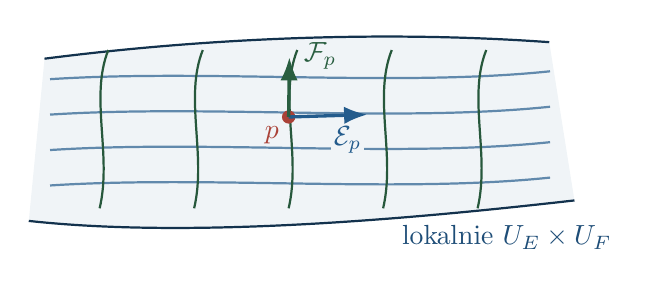
\begin{tikzpicture}[>=Latex,scale=1]
  \fill[manifoldblue!7] (-3.45,-1.15)
    .. controls (-1.35,-1.38) and (1.45,-1.12) .. (3.48,-.89)
    -- (3.16,1.12)
    .. controls (.78,1.29) and (-1.54,1.13) .. (-3.25,.91)
    -- cycle;
  \draw[manifoldblue!55!black,thick] (-3.45,-1.15)
    .. controls (-1.35,-1.38) and (1.45,-1.12) .. (3.48,-.89);
  \draw[manifoldblue!55!black,thick] (-3.25,.91)
    .. controls (-1.54,1.13) and (.78,1.29) .. (3.16,1.12);
  \foreach \y in {-.70,-.25,.20,.65}{
    \draw[manifoldblue!72,thick]
      (-3.18,\y) .. controls (-1.16,\y+.13) and (1.24,\y-.10)
      .. (3.17,\y+.10);
  }
  \foreach \x in {-2.55,-1.35,-.15,1.05,2.25}{
    \draw[manifoldgreen!70!black,thick]
      (\x,-.99) .. controls (\x+.16,-.31) and (\x-.13,.42)
      .. (\x+.11,1.02);
  }
  \fill[manifoldred] (-.15,.17) circle (2.4pt)
     node[below left] {$p$};
  \draw[manifoldblue,very thick,->] (-.15,.17)--++(1.00,.03);
  \node[manifoldblue,fill=manifoldblue!7,inner sep=1pt]
     at (.60,-.12) {$\mathcal E_p$};
  \draw[manifoldgreen!75!black,very thick,->]
     (-.15,.17)--++(.01,.76);
  \node[manifoldgreen!75!black,fill=manifoldblue!7,inner sep=1pt]
     at (.25,.94) {$\mathcal F_p$};
  \node[manifoldblue!85!black] at (2.62,-1.36)
     {lokalnie $U_E\times U_F$};
\end{tikzpicture}
\caption{Schematyczny dwuwymiarowy przekrój układu liści
dwóch prostopadłych rozkładów równoległych.
Niebieskie krzywe przedstawiają kierunki $\mathcal E$,
zielone kierunki $\mathcal F$. Siatka ilustruje lokalny
iloczyn; warunki potrzebne do iloczynu globalnego podaje
Twierdzenie~\ref{thm:de-rham-rozklad}.}
\label{fig:de-rham-liscie}
\end{figure}

\begin{twierdzenie}[Globalny rozkład de Rhama --- wynik zewnętrzny]
\label{thm:de-rham-rozklad}
Niech $(M,g)$ będzie \emph{spójną, zupełną i jednospójną}
rozmaitością riemannowską bez brzegu. Jeśli pełna
holonomia zachowuje właściwą niezerową podprzestrzeń
$W\subset T_pM$, to $M$ jest izometryczna z iloczynem
riemannowskim liści przez $p$ dwóch równoległych
rozkładów odpowiadających $W$ i $W^\perp$.
Powtarzając rozkład, otrzymujemy
\begin{equation}\label{eq:de-rham-kanoniczny}
 (M,g)\cong (\R^k,g_{\mathrm{eukl}})
            \times(M_1,g_1)\times\cdots\times(M_r,g_r),
\end{equation}
gdzie czynniki $M_i$ są zupełne, jednospójne i mają
nieredukowalną nietrywialną holonomię. Czynnik
euklidesowy oraz czynniki nieredukowalne są jednoznaczne
z dokładnością do izometrii i przestawienia tych drugich.
\end{twierdzenie}

W Twierdzeniu~\ref{thm:holonomia-lokalny-produkt}
udowodniliśmy konstrukcję rozkładów, lokalną postać
metryki i zupełność liści. Pozostaje głęboki krok:
wykazanie, że lokalne prostokąty liści sklejają się
jednoznacznie w \emph{globalny} iloczyn tych liści.
Tu zupełność pozwala przedłużać geodezyjne, a
jednospójność usuwa zależność sklejenia od obiegu
pętli. Nie utożsamiamy tego wyjaśnienia z dowodem
kroku globalnego. Dokładne twierdzenie i jego dowód
podaje \href{https://doi.org/10.1007/BF02564308}
{G.~de Rham, \emph{Sur la réductibilité d'un espace de Riemann},
Comment. Math. Helv. 26 (1952), 328--344};
inny szczegółowy dowód daje
\href{https://doi.org/10.1215/ijm/1256059674}
{H.~Wu, \emph{On the de Rham decomposition theorem},
Illinois J. Math. 8 (1964), 291--311}.
Twierdzenie~\ref{thm:de-rham-rozklad} dotyczy metryk
\emph{riemannowskich}; przy sygnaturze nieokreślonej
nie wolno bez dodatkowych warunków przenosić tej wersji.

W szczególności maksymalna przestrzeń nieruchomych
wektorów $(T_pM)^{\operatorname{Hol}_p}$ ma wymiar $k$
czynnika $\R^k$ w~\eqref{eq:de-rham-kanoniczny}.
To wynika z Zasady~\ref{prop:zasada-holonomii}:
baza wektorów nieruchomych przedłuża się do równoległych
pól, które są kierunkami euklidesowymi. Na czynniku
o nietrywialnej nieredukowalnej holonomii nie ma
niezerowego wektora nieruchomego, bo jego prosta byłaby
niezmienniczą podprzestrzenią; w wymiarze jeden
jednospójny zupełny czynnik jest prostą i należy
do części euklidesowej.

\begin{przyklad}[Produkt sfery i prostej]
\label{prz:de-rham-sfera-prosta}
Weźmy $S_R^2\times\R$ z metryką $g_{S_R^2}+\dd t^2$.
Jest to rozmaitość zupełna i jednospójna. Dla pól
pochodzących z obu czynników wzór Koszula
\eqref{eq:koszul} daje
$\nabla_{(X,0)}(Y,0)=(\nabla^{S}_XY,0)$,
$\nabla_{(0,\partial_t)}(0,\partial_t)=0$
oraz zerowe pochodne mieszane. Równanie transportu
rozpada się więc na dwa niezależne równania:
\[
 P_{\gamma}(v,a\partial_t)
   =(P_{\gamma_S}^{S}v,a\partial_t),
 \qquad
 \operatorname{Hol}_{(q,t)}(S_R^2\times\R)
      =SO(T_qS_R^2)\times\{1\}.
\]
Ostatnia równość korzysta z
Przykładu~\ref{prz:holonomia-sfera}; każdą pętlę
na sferze można wykonać przy stałym $t$.
Pole $\partial_t$ jest równoległe. Z~\eqref{eq:stala-krzywizna-tensor}
albo z rozszczepienia koneksji wynika, że płaszczyzny
styczne do sfery mają $K=R^{-2}$, a płaszczyzny
mieszane, zawierające $\partial_t$, mają $K=0$.
To jawny obraz redukowalnej holonomii i dwóch czynników
rozkładu de Rhama.
\end{przyklad}

\begin{przyklad}[Po co potrzebne są założenia globalne?]
\label{prz:de-rham-zalozenia}
Płaski torus i płaska butelka Kleina z
Przykładu~\ref{prz:holonomia-torus-klein} są zupełne,
ale niejednospójne. Ich lokalne metryki mają postać
$\dd x^2+\dd y^2$, natomiast nie są globalnie
izometryczne z $\R^2$: są zwarte. Butelka ma nawet
dwie równoległe proste w każdej przestrzeni stycznej,
lecz nie jest iloczynem dwóch jednowymiarowych
rozmaitości: zwarty iloczyn takich czynników byłby
torusem, a butelka Kleina jest nieorientowalna.

Zupełność też ma znaczenie. Dysk otwarty
$D=\{(x,y):x^2+y^2<1\}\subset\R^2$ z metryką
euklidesową jest jednospójny, płaski i ma dwa stałe
ortogonalne rozkłady. Nie jest jednak globalnym
iloczynem liści poziomego i pionowego przez $0$:
oba liście są przedziałami $(-1,1)$, a ich iloczyn
jest kwadratem, nie dyskiem z metryką produktu.
Geodezyjna radialna kończy się na brzegu w skończonym
czasie, więc $D$ nie jest zupełny.
\end{przyklad}

\begin{uwaga}[Most do teorii Hodge'a]
\label{uwaga:holonomia-bochner}
Na zwartej, spójnej, zorientowanej rozmaitości
riemannowskiej bez brzegu z $\mathrm{Ric}\geq0$
Wniosek~\ref{cor:bochner-vanishing} mówi, że każda
harmoniczna $1$-forma jest równoległa. Odwrotnie
forma równoległa ma $\dd\alpha=0$ i $\delta\alpha=0$,
więc jest harmoniczna. Twierdzenie Hodge'a
z Wniosku~\ref{cor:hodge-de-rham} oraz
Zasada~\ref{prop:zasada-holonomii} dają zatem
\[
 b_1(M)=\dim H^1_{\mathrm{dR}}(M)
       =\dim (T_pM)^{\operatorname{Hol}_p}.
\]
Pierwsza liczba jest topologiczna, ostatnia odczytuje
równoległe kierunki z holonomii. Nie jest to ponowny
dowód kohomologicznego twierdzenia de Rhama.
\end{uwaga}

\section{Druga wariacja energii i pola Jacobiego}
\label{sec:druga-wariacja-jacobi}

Pierwsza wariacja z
Twierdzenia~\ref{thm:pierwsza-wariacja-dlugosci}
mówi, \emph{gdzie} długość może mieć minimum:
krzywa minimalna, po parametryzacji długością łuku,
jest geodezyjną. Drugie różniczkowanie mówi,
\emph{czy w pobliżu geodezyjnej istnieje kierunek},
w którym energia maleje. Krzywizna pojawia się
tu dlatego, że zamiana kolejności dwóch pochodnych
\emph{kowariantnych} wzdłuż wariacji nie jest
na ogół dozwolona bez poprawki $R$.

W całej sekcji $(M,g)$ jest rozmaitością
\emph{riemannowską}, $\nabla$ jej koneksją
Leviego-Civity, a znak $R$ jest ustalony
w~\eqref{eq:riemann-def}. Nie przenosimy
wniosków o minimizowaniu odległości na całe
czasoprzestrzenie lorentzowskie.

\subsection*{Drugie różniczkowanie energii}

Niech $\gamma:[0,\ell]\to M$ będzie geodezyjną
o prędkości $1$, gdzie $\ell>0$, więc $\ell=L_g(\gamma)$.
Rozważmy gładką rodzinę $F(s,t)$ krzywych
o stałych końcach
$F(s,0)=p$, $F(s,\ell)=q$,
$F(0,t)=\gamma(t)$, i jej pole wariacyjne
$V(t)=\partial_sF(0,t)$. W szczególności
$V(0)=V(\ell)=0$. Piszemy $D_t$ oraz $D_s$
na pochodne kowariantne pól wzdłuż powierzchni
parametrów $F$.

\begin{twierdzenie}[Druga wariacja energii]
\label{thm:druga-wariacja-energii}
Dla powyższej wariacji, przy energii
z~\eqref{eq:dlugosc-energia}, zachodzi
\begin{equation}\label{eq:druga-wariacja-energii}
 \left.\frac{\dd^2}{\dd s^2}E_g(F_s)\right|_{s=0}
 =\int_0^\ell\left(
   |D_tV|_g^2-g(R(V,T)T,V)\right)\dd t,
 \qquad T=\dot\gamma.
\end{equation}
Prawą stronę oznaczamy przez $I(V,V)$.
Jej postać dwuliniowa, zwana \emph{formą indeksową}, to
\begin{equation}\label{eq:forma-indeksowa}
 I(V,W)=\int_0^\ell\left(
   g(D_tV,D_tW)-g(R(V,T)T,W)\right)\dd t
\end{equation}
dla pól $V,W$ zerujących się na końcach.
\end{twierdzenie}
\begin{proof}
Oznaczmy na całej powierzchni wariacji
$S=\partial_sF$ i $U=\partial_tF$.
Zgodność koneksji z metryką daje, dla każdego $s$,
\[
 \frac{\dd}{\dd s}E_g(F_s)
 =\int_0^\ell g(D_sU,U)\,\dd t.
\]
Ponieważ $[\partial_s,\partial_t]=0$ i koneksja
nie ma torsji, $D_sU=D_tS$. Po całkowaniu
przez części otrzymujemy \emph{dla całej rodziny}
\begin{equation}\label{eq:pierwsza-wariacja-energii-kow}
 \frac{\dd}{\dd s}E_g(F_s)
 =\bigl[g(S,U)\bigr]_0^\ell
   -\int_0^\ell g(S,D_tU)\,\dd t.
\end{equation}
Końce są nieruchome, więc $S(s,0)=S(s,\ell)=0$;
składnik brzegowy oraz jego pochodna po $s$
znikają. Różniczkujemy pozostałą całkę.
Przy $s=0$ mamy $D_tU=D_tT=0$, gdyż
$\gamma$ jest geodezyjną. Człon zawierający
$D_sS$ znika, bez względu na \emph{przyspieszenie}
wybranej wariacji. Zostaje
\[
 E_g''(0)=-\int_0^\ell
         g(V,D_sD_tU|_{s=0})\,\dd t.
\]
Definicja~\eqref{eq:riemann-def} na polach
wzdłuż $F$ ma tutaj postać
$D_sD_tU-D_tD_sU=R(S,U)U$.
Ponieważ $D_sU=D_tS$, dostajemy krok po kroku
\[
 D_sD_tU=D_t(D_sU)+R(S,U)U
          =D_t^2S+R(S,U)U.
\]
Po podstawieniu $s=0$ jest to
$D_t^2V+R(V,T)T$. Wreszcie reguła iloczynu
i $V(0)=V(\ell)=0$ dają
\[
 -\int_0^\ell g(V,D_t^2V)\,\dd t
 =-\bigl[g(V,D_tV)\bigr]_0^\ell
  +\int_0^\ell|D_tV|_g^2\,\dd t
 =\int_0^\ell|D_tV|_g^2\,\dd t.
\]
To dowodzi~\eqref{eq:druga-wariacja-energii}.
Polaryzacja daje~\eqref{eq:forma-indeksowa};
symetria $I(V,W)=I(W,V)$ wynika również
z symetrii tensora krzywizny, bo
$g(R(V,T)T,W)=g(R(W,T)T,V)$.
\end{proof}

W przeciwieństwie do pierwszej wariacji,
w~\eqref{eq:druga-wariacja-energii} pojawia się
zarówno koszt zmieniania kierunku pola $V$,
czyli $|D_tV|^2$, jak i wkład krzywizny.
Na sferze dodatnia krzywizna odejmuje od
pierwszego składnika; przy ujemnej krzywiźnie
poprzeczne wychylenie kosztuje dodatkową energię.

\begin{figure}[htbp]
\centering
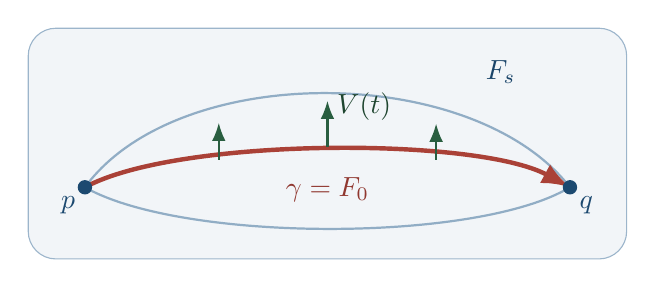
\begin{tikzpicture}[>=Latex,scale=1]
  \fill[manifoldblue!6,rounded corners=10pt]
       (-3.8,-1.45) rectangle (3.8,1.48);
  \draw[manifoldblue!45,rounded corners=10pt]
       (-3.8,-1.45) rectangle (3.8,1.48);
  \coordinate (p) at (-3.08,-.54);
  \coordinate (q) at (3.08,-.54);
  \draw[manifoldblue!50,thick]
       (p) .. controls (-1.9,1.07) and (1.85,1.04) .. (q);
  \draw[manifoldblue!50,thick]
       (p) .. controls (-1.85,-1.24) and (1.9,-1.25) .. (q);
  \draw[manifoldred,ultra thick,->]
       (p) .. controls (-1.9,.10) and (1.90,.10) .. (q);
  \draw[manifoldgreen!75!black,thick,->]
       (-1.38,-.19)--(-1.38,.28);
  \draw[manifoldgreen!75!black,thick,->]
       (0,-.03)--(0,.56);
  \draw[manifoldgreen!75!black,thick,->]
       (1.38,-.19)--(1.38,.27);
  \node[manifoldgreen!55!black,right] at (0,.49) {$V(t)$};
  \fill[manifoldblue!80!black] (p) circle (2.6pt)
       node[below left] {$p$};
  \fill[manifoldblue!80!black] (q) circle (2.6pt)
       node[below right] {$q$};
  \node[manifoldred!85!black] at (0,-.57) {$\gamma=F_0$};
  \node[manifoldblue!75!black] at (2.2,.92) {$F_s$};
\end{tikzpicture}
\caption{Wariacja o nieruchomych końcach: pole $V$ opisuje pierwsze przemieszczenie punktów krzywej $\gamma$. Druga wariacja mierzy zmianę energii przy takim wychyleniu. Rysunek schematyczny; otaczające krzywe nie muszą być geodezyjnymi.}
\label{fig:druga-wariacja-krzywej}
\end{figure}

\begin{stwierdzenie}[Druga wariacja długości]
\label{prop:druga-wariacja-dlugosci}
Przy tych samych założeniach, dla wariacji
regularnych krzywych, zachodzi
\begin{equation}\label{eq:druga-wariacja-dlugosci}
 \left.\frac{\dd^2}{\dd s^2}L_g(F_s)\right|_{s=0}
 = I(V,V)-\int_0^\ell
      g(D_tV,T)^2\,\dd t.
\end{equation}
Jeśli $V$ jest prostopadłe do $T$ w każdym
punkcie, obie drugie wariacje są równe.
\end{stwierdzenie}
\begin{proof}
Przy $s=0$ mamy $|U|=|T|=1$. Zwykłe
różniczkowanie funkcji $\sqrt{h}$ dla
$h(s,t)=g(U,U)$ pokazuje punktowo, że
\[
 \left.\partial_s^2|U|\right|_{s=0}
 =\left.\partial_s^2\frac{|U|^2}{2}\right|_{s=0}
   -\bigl(\left.\partial_s|U|\right|_{s=0}\bigr)^2.
\]
Pierwszy składnik po scałkowaniu daje $E''(0)$.
Ponadto $\partial_s|U||_0=g(D_sU,T)|_0
=g(D_tV,T)$. To daje wzór. Jeżeli
$g(V,T)=0$ na całym $[0,\ell]$, to
$g(D_tV,T)=\frac{\dd}{\dd t}g(V,T)=0$,
bo $D_tT=0$.
\end{proof}

To rozróżnienie jest potrzebne: dla pola
$V=fT$ z $f(0)=f(\ell)=0$ wzór na energię
daje $I(fT,fT)=\int_0^\ell(f')^2\dd t$,
natomiast druga wariacja długości wynosi
zero. Przesuwanie punktów \emph{wzdłuż} tej
samej krzywej zmienia jej parametryzację,
a długość nie zależy od parametryzacji.

\subsection*{Pola Jacobiego: sąsiednie geodezyjne}

\begin{definicja}[Pole Jacobiego]
\index{pole jacobiego@Pole Jacobiego}
\label{def:pole-jacobiego}
Pole wektorowe $J$ wzdłuż geodezyjnej
$\gamma$, z $T=\dot\gamma$, nazywamy
\emph{polem Jacobiego}, jeśli
\begin{equation}\label{eq:jacobi-rownanie}
 D_t^2J+R(J,T)T=0.
\end{equation}
Równanie jest liniowe. Przy naszej konwencji
na sferze $R(J,T)T$ ma zwrot prostopadłego
pola $J$, a więc $D_t^2J=-R(J,T)T$
jest skierowane z powrotem ku geodezyjnej.
\end{definicja}

\begin{twierdzenie}[Pola Jacobiego powstają z geodezyjnych]
\label{thm:jacobi-wariacja-geodezyjnych}
Jeżeli $F(s,t)$ jest wariacją, dla której
każda krzywa $t\mapsto F(s,t)$ jest
geodezyjną z parametrem afinicznym, to
$J=\partial_sF|_{s=0}$ spełnia
\eqref{eq:jacobi-rownanie}. Odwrotnie:
każde pole Jacobiego wzdłuż $\gamma$ na
zwartym przedziale jest polem wariacyjnym
pewnej rodziny geodezyjnych.
\end{twierdzenie}
\begin{proof}
Niech znów $S=\partial_sF$ i $U=\partial_tF$.
Teraz $D_tU=0$ dla \emph{każdego} $s$,
więc $D_sD_tU=0$. Obliczenie wykonane
w dowodzie Twierdzenia~\ref{thm:druga-wariacja-energii}
daje
\[
 0=D_t^2S+R(S,U)U.
\]
Przy $s=0$ jest to równanie Jacobiego.

Dla odwrotności wybierzmy
$A=J(0)$ i $B=D_tJ(0)$.
Weźmy krzywą $p_s$ z $p_0=\gamma(0)$,
$\dot p_0=A$. Niech $P_s:T_{p_0}M\to T_{p_s}M$
będzie transportem równoległym wzdłuż $p_s$
i połóżmy $v_s=P_s(T(0)+sB)$.
Dla małych $s$ rodzina geodezyjnych
$F(s,t)=\gamma_{p_s,v_s}(t)$ istnieje na
całym zadanym zwartym przedziale: rozwiązania
ODE zależą gładko od danych bliskich danym
$\gamma$, a skończona liczba lokalnych
przedłużeń pokrywa przedział.
Jej pole $\widetilde J=\partial_sF|_0$
ma $\widetilde J(0)=A$ oraz, z
$D_t\widetilde J=D_sU$,
$D_t\widetilde J(0)=D_s v_s|_0=B$.
W równoległej ramie wzdłuż $\gamma$
równanie~\eqref{eq:jacobi-rownanie} staje się
układem liniowych ODE drugiego rzędu
$y''+A(t)y=0$. Jednoznaczność rozwiązania
przy ustalonych $J(0),D_tJ(0)$ daje
$\widetilde J=J$ na całym przedziale.
\end{proof}

Pole Jacobiego mierzy więc, jak zmienia się
położenie punktu na geodezyjnej, gdy nieznacznie
zmieniamy jej \emph{punkt startowy lub prędkość}.
Nie zakładamy tu, że końce są nieruchome;
wariacje geodezyjnych o ustalonych obu końcach
mogą nie istnieć poza szczególnymi sytuacjami.

\begin{definicja}[Punkty sprzężone]
\index{punkty sprzezone@Punkty sprzężone}
\label{def:punkty-sprzezone}
Parametry $0$ i $c>0$, a także odpowiadające
im punkty $p=\gamma(0)$ i $\gamma(c)$
\emph{wzdłuż wybranej geodezyjnej}, nazywamy
\emph{sprzężonymi}, jeśli istnieje niezerowe
pole Jacobiego $J$ spełniające
$J(0)=J(c)=0$. Gdy geodezyjna sama się
przecina, sformułowanie przez parametry
usuwa niejednoznaczność.
\end{definicja}

\begin{stwierdzenie}[Punkty sprzężone i odwzorowanie wykładnicze]
\label{prop:jacobi-dexp}
Jeżeli $\gamma(t)=\exp_p(tv)$ oraz $v=T(0)$,
to dla $w\in T_pM$ pole powstające przez
zmianę prędkości początkowej $v+sw$ ma postać
\begin{equation}\label{eq:jacobi-dexp}
 J_w(t)=\left.\partial_s\exp_p(t(v+sw))\right|_{s=0}
       =\dd(\exp_p)_{tv}(tw),
 \qquad J_w(0)=0,\quad D_tJ_w(0)=w.
\end{equation}
W konsekwencji $\gamma(c)$ jest sprzężony z $p$
wzdłuż $\gamma$ wtedy i tylko wtedy, gdy
$\dd(\exp_p)_{cv}$ ma niezerowe jądro.
\end{stwierdzenie}
\begin{proof}
Różniczkujemy rodzinę geodezyjnych
$t\mapsto\exp_p(t(v+sw))$ po $s$ i stosujemy
regułę łańcuchową; daje to pierwsze dwie
równości. Wszystkie krzywe startują z $p$,
więc $J_w(0)=0$. Ich prędkości początkowe
są równe $v+sw$, stąd $D_tJ_w(0)=w$.
Każde pole Jacobiego zerujące się w $0$
jest jednym z $J_w$, ponieważ jego
początkowa pochodna $w$ wyznacza je jednoznacznie.
Dla $c>0$ warunek $J_w(c)=0$ jest równoważny
$\dd(\exp_p)_{cv}(cw)=0$. Ponieważ
$w\ne0$ dokładnie wtedy, gdy $cw\ne0$,
otrzymujemy tezę.
\end{proof}

Różniczka $\dd\exp_p$ pokazuje zatem,
kiedy geodezyjne startujące z $p$ zaczynają
się \emph{ogniskować}: początkowo różne kierunki
mogą w pierwszym przybliżeniu prowadzić
do tego samego punktu. W punkcie sprzężonym
normalne współrzędne z centrum $p$ tracą
lokalną odwracalność wzdłuż tego promienia.

\subsection*{Trzy znaki krzywizny i przykłady}

Na przestrzeni o stałej krzywiźnie sekcyjnej
$\kappa$, z~\eqref{eq:stala-krzywizna-tensor} wynika,
że dla jednostkowego $T$ i prostopadłego
równoległego pola $E$ mamy
$R(E,T)T=\kappa E$.
Jeżeli $J(t)=f(t)E(t)$, równanie Jacobiego
redukuje się do zwykłego równania
\begin{equation}\label{eq:jacobi-stala-krzywizna}
 f''+\kappa f=0,
 \qquad f(0)=0,\quad f'(0)=1.
\end{equation}
Jego rozwiązania dla trzech znaków krzywizny to
\begin{equation}\label{eq:jacobi-trzy-krzywizny}
 f_\kappa(t)=
 \begin{cases}
  \dfrac{\sin(\sqrt\kappa\,t)}{\sqrt\kappa},
       &\kappa>0,\\[5pt]
  t,&\kappa=0,\\[3pt]
  \dfrac{\sinh(\sqrt{-\kappa}\,t)}{\sqrt{-\kappa}},
       &\kappa<0.
 \end{cases}
\end{equation}
Sprawdzamy to bez skrótu: dla $\kappa>0$
dwie pochodne sinusa dają $f''=-\kappa f$;
analogicznie $\sinh$ daje $f''=(-\kappa)f$,
więc $f''+\kappa f=0$; wszystkie trzy wzory
mają $f(0)=0$, $f'(0)=1$.
Składowa styczna pola Jacobiego ma natomiast
postać $(a+bt)T$, bo $R(T,T)T=0$.
Niezerowa taka składowa nie może znikać
w dwóch różnych chwilach. O punktach
sprzężonych decydują więc składowe poprzeczne.

\begin{przyklad}[Sfera o promieniu $R$]
\label{prz:jacobi-sfera}
Na $S_R^n$, $n\geq2$ i $R>0$, mamy $\kappa=1/R^2$.
Dla $0\ne w\perp v$, po równoległym przesunięciu
$w$ wzdłuż jednostkowej geodezyjnej, dostajemy
\[
 J_w(t)=R\sin(t/R)\,P_t w.
\]
Pole startuje od zera, rośnie, a następnie
znika ponownie przy $t=\pi R$, czyli w antypodzie.
Istnieje $n-1$ niezależnych kierunków $w$,
więc jest to punkt sprzężony krotności $n-1$.
Geometrycznie: różne wielkie półokręgi
wychodzą z $p$ i spotykają się w $-p$.
Na łuku dłuższym niż $\pi R$ można zobaczyć
utratę minimalności bez żadnego ogólnego
twierdzenia. Dla $\ell>\pi R$ weźmy
równoległe jednostkowe pole normalne $E$
i $V(t)=\sin(\pi t/\ell)E(t)$.
Wtedy $V(0)=V(\ell)=0$ i, z formy indeksowej,
\begin{equation}\label{eq:jacobi-sfera-indeks}
 I(V,V)
 =\int_0^\ell\left[\frac{\pi^2}{\ell^2}
                   \cos^2\!\left(\frac{\pi t}{\ell}\right)
       -\frac1{R^2}\sin^2\!\left(\frac{\pi t}{\ell}\right)
                    \right]\dd t
 =\frac\ell2\left(\frac{\pi^2}{\ell^2}
                     -\frac1{R^2}\right)<0.
\end{equation}
Taki łuk nie może być minimalny.
Przy $\ell=\pi R$ wybrane pole daje $I=0$,
a mimo to półokrąg \emph{jest} minimalny:
zero drugiej wariacji samo nie rozstrzyga sprawy.
\end{przyklad}

\begin{figure}[htbp]
\centering
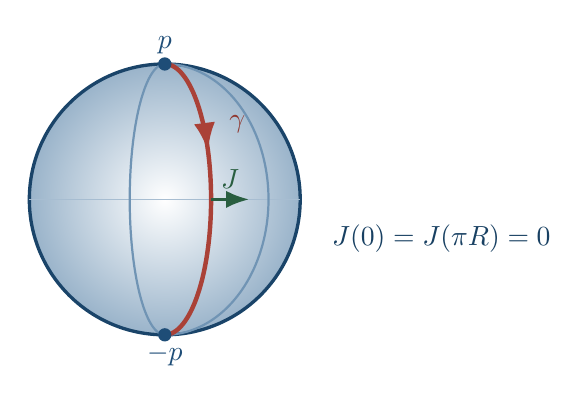
\begin{tikzpicture}[>=Latex]
 \shade[inner color=white,outer color=manifoldblue!46] (0,0) circle (1.72);
 \draw[manifoldblue!75!black,very thick] (0,0) circle (1.72);
 \draw[manifoldblue!40] (-1.72,0)--(1.72,0);
 \foreach \b in {-15,50}
  \draw[manifoldblue!65,thick] plot[domain=0:180,samples=90]
    ({1.72*sin(\b)*sin(\x)},{1.72*cos(\x)});
 \draw[manifoldred,ultra thick,postaction={decorate,decoration={markings,
   mark=at position .34 with {\arrow{Latex}}}}]
  plot[domain=0:180,samples=90] ({1.72*sin(20)*sin(\x)},{1.72*cos(\x)});
 \draw[manifoldgreen!75!black,very thick,->]
  ({1.72*sin(20)},0)--({1.72*sin(20)+.3*1.72*cos(20)},0)
  node[midway,above] {$J$};
 \fill[manifoldblue!85!black] (0,1.72) circle (2.4pt) node[above] {$p$};
 \fill[manifoldblue!85!black] (0,-1.72) circle (2.4pt) node[below] {$-p$};
 \node[manifoldred!85!black] at (.92,.95) {$\gamma$};
 \node[manifoldblue!70!black,anchor=west] at (2,-.5) {$J(0)=J(\pi R)=0$};
\end{tikzpicture}
\caption{Rzut wielkich półokręgów na sferze oglądanej prostopadle do osi biegunowej.
Półokręgi spotykają się w antypodzie. Pole Jacobiego, otrzymane przez zmianę
długości geograficznej, znika przy $p$ i $-p$. Zielona strzałka pokazuje jego
rzut w punkcie równika, w umownej skali.}
\label{fig:jacobi-sfera-ogniskowanie}
\end{figure}

\begin{przyklad}[Płaszczyzna i trzy modele hiperboliczne]
\label{prz:jacobi-plaska-hiperboliczna}
W $\R^n$ pole poprzeczne z $J(0)=0$
i $D_tJ(0)=w$ ma postać $J(t)=tw$,
przy identyfikacji przestrzeni stycznych przez
transport równoległy. Dla $w\ne0$ nie znika już przy $t>0$.
W przestrzeni o $K=-1$ analogicznie
$J(t)=\sinh(t)P_tw$, więc sąsiednie geodezyjne
rozchodzą się szybciej. Ponadto dla
$V=V^\parallel+V^\perp$ z zerowymi końcami
\[
 I(V,V)=\int_0^\ell
        \bigl(|D_tV|^2+|V^\perp|^2\bigr)\dd t>0
 \quad\text{dla }V\ne0.
\]
Nie ma punktów sprzężonych. Dotyczy to
\emph{tej samej} przestrzeni hiperbolicznej
zapisanej jako półprzestrzeń, kula Poincarégo
lub hiperboloida; metryki i izometrie między
nimi podano w~\ref{prz:trzy-modele-hiperboliczne},
a $K=-1$ obliczono w
Stwierdzeniu~\ref{prop:krzywizna-trzy-modele-hiperboliczne}.
Wzór dodatniej formy mówi o \emph{lokalnej}
stabilności. Globalną minimalność i jedyność
geodezyjnych w tych trzech modelach potwierdzają
odległości~\eqref{eq:odleglosci-modele-hiperboliczne}.
\end{przyklad}

\subsection*{Co naprawdę wynika dla krzywej minimalnej?}

\begin{twierdzenie}[Warunki konieczne i punkty sprzężone]
\label{thm:minimalna-bez-sprzezonego-wewnatrz}
Jeżeli ciągła, odcinkami $C^1$ krzywa
$\gamma:[0,\ell]\to M$, $\ell>0$, minimalizuje
długość między $p$ i $q$ i jest parametryzowana
długością łuku, to:
\begin{enumerate}[label=\textup{(\roman*)}]
 \item $\gamma$ jest geodezyjną;
 \item $I(V,V)\geq0$ dla każdego gładkiego pola
       $V$ wzdłuż $\gamma$ z $V(0)=V(\ell)=0$;
 \item żaden punkt $\gamma(c)$ dla
       $0<c<\ell$ nie jest sprzężony z $p$
       wzdłuż $\gamma$.
\end{enumerate}
Punkt końcowy $q$ \emph{może} być sprzężony z $p$.
\end{twierdzenie}
\begin{proof}
Każdy podłuk $\gamma$ również minimalizuje długość:
jego skrócenie skróciłoby całą drogę. Ustalmy punkt
$\gamma(t_0)$ i jego małe otoczenie normalne. Dla
$t$ bliskich $t_0$ krzywa pozostaje w tym otoczeniu.
Warunek równości w dowodzie lokalnej minimalności
promieni (Twierdzenie~\ref{thm:lokalna-minimalnosc-geodezyjnej})
wymusza, aby każdy z dwóch podłuków wychodzących
z $\gamma(t_0)$ był radialny. Parametr długości łuku
nadaje im prędkość $1$. Są więc gładkimi geodezyjnymi
po obu stronach $t_0$, a argument o braku narożników
z dowodu Twierdzenia~\ref{thm:pierwsza-wariacja-dlugosci}
zrównuje ich prędkości w $t_0$. Jednoznaczność ODE
skleja je w jedną gładką geodezyjną. Na końcach stosujemy
argument jednostronny. To dowodzi (i), bez zakładania
gładkości minimalnej krzywej z góry.
Sama druga wariacja nie zastępuje tego kroku:
stosujemy jej wzór dopiero \emph{na geodezyjnej}.

Niech $F_s$ będzie dowolną wariacją z nieruchomymi
końcami. Dla krzywych określonych na
$[0,\ell]$ nierówność~\eqref{eq:energia-cauchy}
oraz minimalność $\gamma$ dają
\[
 E_g(F_s)\geq\frac{L_g(F_s)^2}{2\ell}
             \geq\frac{\ell^2}{2\ell}
             =E_g(\gamma).
\]
Energia ma więc minimum przy $s=0$, skąd
$E_g''(0)\geq0$. Każde gładkie pole $V$
zerujące się na końcach można zrealizować
przez $F(s,t)=\exp_{\gamma(t)}(sV(t))$
przy dostatecznie małym $s$; zwartość
przedziału zapewnia wspólną dziedzinę.
Wzór~\eqref{eq:druga-wariacja-energii}
daje (ii).

Dowiedźmy (iii) przez sprzeczność, pokazując
konkretny kierunek ujemnej drugiej wariacji.
Załóżmy, że $0<c<\ell$ i istnieje niezerowe
pole Jacobiego $J$ z $J(0)=J(c)=0$.
Przedłużmy je przez zero na $[c,\ell]$;
powstałe ciągłe pole oznaczmy $\widehat J$.
Jest gładkie oddzielnie po obu stronach $c$.
Z jednoznaczności równania Jacobiego wynika
$D_tJ(c)\ne0$, gdyż w przeciwnym razie
oba dane $J(c),D_tJ(c)$ byłyby zerowe.

Całkując przez części na $[0,c]$ i używając
równania Jacobiego, dla każdego pola $W$
o zerowych końcach otrzymujemy
\begin{equation}\label{eq:jacobi-przedluzone-indeks}
 I(\widehat J,W)
 =\bigl[g(D_tJ,W)\bigr]_0^c
 =g(D_tJ(c),W(c)),
 \qquad I(\widehat J,\widehat J)=0.
\end{equation}
Wybierzmy gładkie $W$ z $W(0)=W(\ell)=0$
i $W(c)=-D_tJ(c)$, na przykład przez
pomnożenie pola z lokalnej równoległej ramy
przez funkcję z nośnikiem blisko $c$.
Wtedy $I(\widehat J,W)=-|D_tJ(c)|^2<0$.
Dla dostatecznie małego $\varepsilon>0$
\[
 I(\widehat J+\varepsilon W,
   \widehat J+\varepsilon W)
 =-2\varepsilon|D_tJ(c)|^2
       +\varepsilon^2 I(W,W)<0.
\]
Wygładzamy $\widehat J$ w małym otoczeniu $c$
w równoległej ramie. Ponieważ jest ciągłe,
odcinkami gładkie i ma ograniczoną pochodną,
można to zrobić tak, by pole i jego pierwsza
pochodna zbliżały się w całce z kwadratu,
zachowując zerowe końce. Na zwartym przedziale
współczynniki krzywizny są ograniczone,
więc całka~\eqref{eq:forma-indeksowa}
zmienia się wtedy dowolnie mało. Otrzymujemy
\emph{gładkie} pole z $I<0$, sprzeczne z (ii).
Zatem punkt sprzężony nie może leżeć
we wnętrzu odcinka minimalnego.
Wreszcie przy $c=\ell$ wyraz $W(c)$ w
\eqref{eq:jacobi-przedluzone-indeks} musi
być zerowy, więc ten argument nie daje
ujemnego kierunku. Przykład sfery powyżej
pokazuje, że końcowy punkt sprzężony jest
możliwy.
\end{proof}

Brak punktów sprzężonych jest \emph{konieczny}
dla minimalności na otwartym odcinku,
ale sam nie zapewnia globalnie najkrótszej drogi.
Widać to nawet przy zerowej krzywiźnie.

\begin{przyklad}[Płaski walec: brak sprzężenia nie wystarcza]
\label{prz:jacobi-plaski-walec}
Na walcu $S_R^1\times\R$ z metryką
$g=R^2\dd\theta^2+\dd z^2$ poziomy łuk
$\gamma(t)=(t/R,0)$, $0\leq t\leq\ell$,
jest jednostkową geodezyjną. W lokalnych
współrzędnych metryka ma stałe współczynniki,
więc $R(X,Y)Z=0$; pola Jacobiego o zerowym
początku mają postać $tP_tw$ i dla $w\ne0$ nie znikają
ponownie. Gdy $\pi R<\ell<2\pi R$, drugi
łuk tego samego okręgu łączy te same końce
i ma długość $2\pi R-\ell<\ell$.
Geodezyjna przestaje zatem być globalnie
minimalna \emph{bez punktu sprzężonego}.
Przeszkodą jest tu globalne zawinięcie walca,
którego lokalne równanie Jacobiego nie widzi.
\end{przyklad}

\begin{figure}[htbp]
\centering
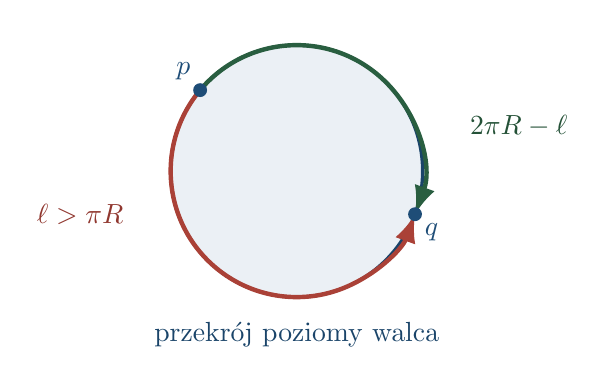
\begin{tikzpicture}[>=Latex,scale=1]
  \fill[manifoldblue!9] (0,0) circle (1.60);
  \draw[manifoldblue!75!black,very thick] (0,0) circle (1.60);
  \draw[manifoldred,ultra thick,->]
       (140:1.60) arc[start angle=140,end angle=340,radius=1.60];
  \draw[manifoldgreen!75!black,ultra thick,->]
       (140:1.60) arc[start angle=140,end angle=-20,radius=1.60];
  \fill[manifoldblue!85!black] (140:1.60) circle (2.5pt)
       node[above left] {$p$};
  \fill[manifoldblue!85!black] (-20:1.60) circle (2.5pt)
       node[below right] {$q$};
  \node[manifoldred!85!black] at (-2.75,-.55)
       {$\ell>\pi R$};
  \node[manifoldgreen!65!black] at (2.82,.57)
       {$2\pi R-\ell$};
  \node[manifoldblue!75!black] at (0,-2.08)
       {przekrój poziomy walca};
\end{tikzpicture}
\caption{Ten sam okrąg oglądany jako poziomy przekrój płaskiego walca. Między $p$ i $q$ dłuższy łuk (czerwony) jest geodezyjną bez punktów sprzężonych, lecz krótszy łuk (zielony) wygrywa globalnie.}
\label{fig:jacobi-walec-dwa-luki}
\end{figure}

Podsumowując logiczną kolejność:
\emph{minimalność długości} wymusza równanie
geodezyjnej przez pierwszą wariację, a następnie
nieujemność formy indeksowej przez drugą.
Pola Jacobiego opisują sąsiednie geodezyjne
i wskazują pierwszą przeszkodę w utrzymaniu
minimalności na coraz dłuższych odcinkach.
Na sferze przeszkodą jest ogniskowanie;
na walcu może nią być topologia, choć
ogniskowania w ogóle nie ma.

Z tym rozróżnieniem łączy się Sekcja~\ref{sec:geodezyjne-miejsce-ciecia}.
Jeżeli $u\in T_pM$ jest jednostkowy, to dla każdego
$0<t<c_p(u)$ odcinek geodezyjnej można przedłużyć
do odcinka minimalnego. Twierdzenie~\ref{thm:minimalna-bez-sprzezonego-wewnatrz}
wyklucza więc sprzężenie przed czasem cięcia, a
Stwierdzenie~\ref{prop:jacobi-dexp} daje w tych punktach
odwracalność $\dd\exp_p$. W samym miejscu cięcia
występuje sprzężenie wzdłuż wybranej geodezyjnej lub
spotykają się co najmniej dwie geodezyjne minimalne;
możliwości te mogą
zachodzić jednocześnie (Wniosek~\ref{cor:ciecie-sprzezenie-lub-dwa-promienie}).
Kres dolny czasów cięcia spośród kierunków to
$\operatorname{inj}(p)$ na mocy
Twierdzenia~\ref{thm:ciecie-promien-injektywnosci}.
Na sferze oba mechanizmy występują w antypodzie
(Przykład~\ref{prz:ciecie-sfera}), a na płaskim torusie
cięcie wynika ze spotkania dróg minimalnych bez
sprzężenia (Przykład~\ref{prz:ciecie-torus}).

\section{Twierdzenia porównawcze}
\label{sec:twierdzenia-porownawcze}

Znamy już dokładne rozwiązania równania Jacobiego
przy stałej krzywiźnie. Co można powiedzieć, gdy
krzywizna zmienia się z punktu na punkt, ale znamy
jej górną albo dolną granicę? \emph{Porównanie}
z modelem o stałej krzywiźnie zamienia nierówność
dotyczącą $R$ w informację o geodezyjnych,
odległościach, objętości lub topologii.

Przez tę sekcję zakładamy $n=\dim M\geq2$
i metrykę riemannowską. Dla $\kappa\in\R$
oznaczmy
\begin{equation}\label{eq:porownanie-s-kappa}
 s_\kappa(r)=
 \begin{cases}
  \sin(\sqrt\kappa\,r)/\sqrt\kappa,&\kappa>0,\\
  r,&\kappa=0,\\
  \sinh(\sqrt{-\kappa}\,r)/\sqrt{-\kappa},&\kappa<0,
 \end{cases}
 \qquad c_\kappa(r)=\frac{s_\kappa'(r)}{s_\kappa(r)}.
\end{equation}
To funkcja z~\eqref{eq:jacobi-trzy-krzywizny}:
$s_\kappa''+\kappa s_\kappa=0$,
$s_\kappa(0)=0$, $s_\kappa'(0)=1$.
Ilorazu $c_\kappa$ używamy tylko tam, gdzie
$s_\kappa>0$; dla $\kappa>0$ oznacza to
$0<r<\pi/\sqrt\kappa$. Dla $\kappa=0$
mamy $c_0=1/r$, a dla $\kappa=-1$
mamy $c_{-1}=\coth r$.

\subsection*{Lemat indeksowy i porównanie Raucha}

Kluczowy krok jest wariacyjną własnością pola
Jacobiego. Piszemy $\mathsf K_t(X)=R(X,T)T$
na podprzestrzeni prostopadłej do $T=\dot\gamma$.
Ten operator jest symetryczny; jego forma
kwadratowa jest krzywizną sekcyjną płaszczyzny
rozpiętej przez $X,T$ razy $|X|^2$.

\begin{lemat}[Indeksowy]
\label{lem:indeksowy-porownanie}
Niech $\gamma:[0,b]\to M$ będzie jednostkową
geodezyjną bez punktu sprzężonego z $\gamma(0)$
na $(0,b]$. Niech $J$ będzie prostopadłym
polem Jacobiego z $J(0)=0$. Spośród wszystkich
ciągłych, odcinkami gładkich pól normalnych $X$ z
$X(0)=0$ i $X(b)=J(b)$ pole $J$ minimalizuje
formę indeksową na $[0,b]$:
\begin{equation}\label{eq:lemat-indeksowy}
 I_b(X,X)\geq I_b(J,J)
       =g(D_tJ(b),J(b)).
\end{equation}
\end{lemat}
\begin{proof}
Wybierzmy równoległą bazę ortonormalną
normalną do $T$ i zapisujmy pola przez
kolumny w $\R^{n-1}$. Niech $A(t)$ będzie
macierzą pól Jacobiego spełniających
$A(0)=0$ i $A'(0)=\mathrm{Id}$.
Każda kolumna spełnia
$A''+\mathsf K A=0$, gdzie $\mathsf K$
jest symetryczną macierzą. Brak punktów
sprzężonych oznacza, że $A(t)$ jest odwracalna
dla $0<t\leq b$: wektor z jądra $A(t)$
wyznaczałby niezerowe pole Jacobiego zerujące
się także w $t$.

Połóżmy $H=A'A^{-1}$. Najpierw sprawdźmy,
że $H$ jest symetryczna. Macierz Wrońskiego
$A^{\mathsf T}A'-A'^{\mathsf T}A$ ma pochodną
$A^{\mathsf T}A''-A''^{\mathsf T}A=0$,
bo $A''=-\mathsf K A$ i $\mathsf K^{\mathsf T}
=\mathsf K$. W zerze Wroński znika, więc
znika wszędzie. Mnożenie przez
$(A^{-1})^{\mathsf T}$ z lewej i $A^{-1}$
z prawej daje $H=H^{\mathsf T}$.
Różniczkując $H$ i korzystając z równania
Jacobiego, otrzymujemy \emph{równanie Riccatiego}
\begin{equation}\label{eq:jacobi-riccati}
 H'=A''A^{-1}-A'A^{-1}A'A^{-1}
    =-\mathsf K-H^2.
\end{equation}

Napiszmy $X=J+Z$; pole $Z$ znika na obu
końcach. Całkowanie przez części i równanie
Jacobiego dają $I_b(J,Z)=0$ oraz
$I_b(J,J)=[g(D_tJ,J)]_0^b$.
Z~\eqref{eq:jacobi-riccati} i symetrii $H$
wynika z kolei, dla $0<\varepsilon<b$,
\[
 \int_\varepsilon^b|Z'-HZ|^2\,\dd t
 =I_{[\varepsilon,b]}(Z,Z)
   -[\langle HZ,Z\rangle]_{\varepsilon}^{b}.
\]
Istotnie rozwijamy kwadrat i zastępujemy
$2\langle HZ,Z'\rangle$ wyrażeniem
$\frac{\dd}{\dd t}\langle HZ,Z\rangle-\langle H'Z,Z\rangle$;
pozostałe $H'+H^2$ to $-\mathsf K$.
Ponieważ $A(t)=t\mathrm{Id}+O(t^3)$,
to $H(t)=t^{-1}\mathrm{Id}+O(t)$.
Dla odcinkami gładkiego $Z$ z $Z(0)=0$
mamy $Z(t)=O(t)$, zatem wyraz brzegowy
przy $\varepsilon\downarrow0$ dąży do zera.
W rezultacie
\[
 I_b(Z,Z)=\int_0^b|Z'-HZ|^2\,\dd t\geq0.
\]
Razem z $I_b(X,X)=I_b(J,J)+I_b(Z,Z)$
daje to obie części~\eqref{eq:lemat-indeksowy}.
\end{proof}

Najpierw podajemy wygodną wersję Raucha:
porównujemy wszystkie płaszczyzny poprzeczne
obu geodezyjnych. Ta wersja wystarcza do poniższych
zastosowań; dowód używa właśnie podanego porównania
dla każdej pary kierunków poprzecznych.

\begin{twierdzenie}[Porównanie Raucha]
\label{thm:rauch-porownanie}
Niech $\gamma_i:[0,b)\to M_i$, $i=1,2$,
będą jednostkowymi geodezyjnymi w rozmaitościach
tego samego wymiaru. Załóżmy, że dla każdej
chwili $t$ i dowolnych jednostkowych wektorów
$X_i\perp\dot\gamma_i(t)$ zachodzi
\[
 K_1(\dot\gamma_1\wedge X_1)
 \leq K_2(\dot\gamma_2\wedge X_2).
\]
Niech normalne pola Jacobiego $J_i$ spełniają
$J_i(0)=0$ i
$|D_tJ_1(0)|=|D_tJ_2(0)|>0$.
Jeśli wzdłuż $\gamma_2$ nie ma punktu
sprzężonego z początkiem w $(0,b)$, to
\begin{equation}\label{eq:rauch-nierownosc}
 |J_1(t)|\geq |J_2(t)|,
 \qquad 0<t<b.
\end{equation}
W szczególności niższa krzywizna sekcyjna
pozwala geodezyjnym rozchodzić się co najmniej
tak szybko, jak w przestrzeni bardziej zakrzywionej.
\end{twierdzenie}
\begin{proof}
Przy ustalonym $t$ przed ewentualnym pierwszym
zerem $J_1$ połóżmy
$Y_i(s)=J_i(s)/|J_i(t)|$ dla $0\leq s\leq t$.
Wybierzmy izometrię między przestrzeniami
normalnymi obu geodezyjnych, przenoszoną
równolegle wzdłuż $s$, która przy $s=t$
odwzorowuje $Y_1(t)$ na $Y_2(t)$.
Niech $\widetilde Y_1$ będzie obrazem całego
pola $Y_1$ wzdłuż $\gamma_2$. Przenoszenie
zachowuje normy pól i ich pochodnych.
Założona nierówność krzywizn daje więc,
po odjęciu członów krzywizny w~\eqref{eq:forma-indeksowa},
\[
 I_{1,t}(Y_1,Y_1)
 \geq I_{2,t}(\widetilde Y_1,\widetilde Y_1).
\]
Pola $\widetilde Y_1$ oraz $Y_2$ mają te
same wartości: zero w $0$ i ten sam wektor
jednostkowy w $t$. Lemat~\ref{lem:indeksowy-porownanie}
dla $\gamma_2$ daje
$I_{2,t}(\widetilde Y_1,\widetilde Y_1)
\geq I_{2,t}(Y_2,Y_2)$.
Ponieważ $Y_i$ jest polem Jacobiego,
\eqref{eq:lemat-indeksowy} przekształca ten
łańcuch nierówności w
\[
 \frac{\dd}{\dd t}\log|J_1(t)|
 =\frac{g(D_tJ_1,J_1)}{|J_1|^2}
 \geq\frac{g(D_tJ_2,J_2)}{|J_2|^2}
 =\frac{\dd}{\dd t}\log|J_2(t)|.
\]
Całkujemy od $\varepsilon$ do $t$.
Przy $\varepsilon\downarrow0$ zachodzi
$|J_i(\varepsilon)|/\varepsilon
\to|D_tJ_i(0)|$, więc iloraz początkowy
dąży do $1$. Otrzymujemy~\eqref{eq:rauch-nierownosc}.
Jeżeli $J_1$ miałoby pierwsze zero przed $b$,
ta nierówność i ciągłość dawałyby tam
$0\geq|J_2|>0$, sprzeczność. Dowód obejmuje
zatem cały wskazany przedział.
\end{proof}

\begin{wniosek}[Porównanie z modelem]
\label{cor:rauch-model}
Jeżeli $K_M\leq\kappa$, to dla normalnego
pola Jacobiego $J(0)=0$, $D_tJ(0)=w$ mamy
\begin{equation}\label{eq:jacobi-gorne-K}
 |J(r)|\geq s_\kappa(r)|w|
\end{equation}
do pierwszego zera $s_\kappa$ (bez ograniczenia
czasu, gdy $\kappa\leq0$). Nie ma więc
punktu sprzężonego \emph{przed} tym zerem.
Jeżeli $K_M\geq\kappa$, nierówność jest
odwrotna aż do pierwszego punktu sprzężonego
w $M$ i pierwszego zera $s_\kappa$.
\end{wniosek}
\begin{proof}
Jako drugą przestrzeń w
Twierdzeniu~\ref{thm:rauch-porownanie}
weźmy model o stałej krzywiźnie $\kappa$.
Jego normalne pole ma długość
$s_\kappa(r)|w|$, zgodnie z
\eqref{eq:jacobi-trzy-krzywizny}.
Przy odwrotnym ograniczeniu krzywizny
zamieniamy role $M$ i modelu; przed
pierwszym punktem sprzężonym w $M$ spełniony
jest warunek lematu indeksowego.
\end{proof}

\begin{figure}[htbp]
\centering
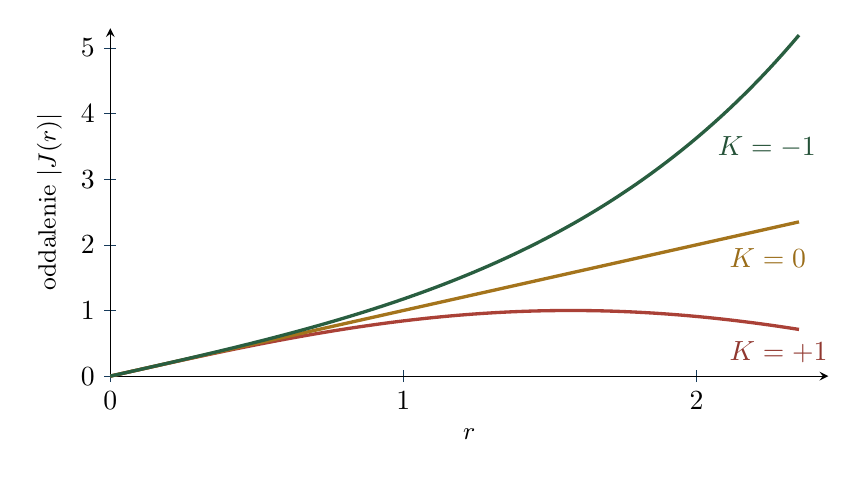
\begin{tikzpicture}
\begin{axis}[
 width=10.7cm,height=6.0cm,
 axis lines=left,
 xmin=0,xmax=2.45,ymin=0,ymax=5.3,
 xtick={0,1,2},ytick={0,1,2,3,4,5},
 xlabel={$r$},ylabel={oddalenie $|J(r)|$},
 tick style={manifoldblue!65!black},
 label style={font=\small},
 clip=false]
 \addplot[manifoldred,very thick,domain=0:2.35,samples=90]
    {sin(deg(x))};
 \addplot[manifoldgold!80!black,very thick,domain=0:2.35]
    {x};
 \addplot[manifoldgreen!75!black,very thick,domain=0:2.35,samples=90]
    {(exp(x)-exp(-x))/2};
 \node[manifoldred!85!black,anchor=west]
    at (axis cs:2.08,.36) {$K=+1$};
 \node[manifoldgold!75!black,anchor=west]
    at (axis cs:2.08,1.80) {$K=0$};
 \node[manifoldgreen!65!black,anchor=west]
    at (axis cs:2.04,3.48) {$K=-1$};
\end{axis}
\end{tikzpicture}
\caption{W modelach o krzywiznach $+1,0,-1$ zerowe początkowe wychylenie i jednostkowa pochodna $D_rJ(0)$ dają odpowiednio $|J(r)|=\sin r$, $r$, $\sinh r$. Wykres pokazuje zakres $0\leq r\leq2{,}35$; pierwsze ponowne zero na sferze występuje później, przy $r=\pi$.}
\label{fig:rauch-porownanie-jacobiego}
\end{figure}

\subsection*{Porównanie hesjanu odległości}

W tej podsekcji zakładamy, że $(M,g)$ jest spójna
i zupełna. Najpierw uzasadnijmy, gdzie odległość
$r(x)=d_g(p,x)$ jest gładka.

\begin{lemat}[Czas cięcia i współrzędne biegunowe]
\label{lem:czas-ciecia-polar}
Dla $\theta\in S_pM$ połóżmy
\[
 c(\theta)=\sup\{t>0:d_g(p,\exp_p(t\theta))=t\}
 \in(0,\infty],\qquad
 C_p=\{\exp_p(c(\theta)\theta):c(\theta)<\infty\}.
\]
Zbiór $C_p$ nazywamy \emph{zbiorem cięcia} punktu $p$.
Odwzorowanie biegunowe $F(t,\theta)=\exp_p(t\theta)$
jest dyfeomorfizmem zbioru
$D=\{(t,\theta):0<t<c(\theta)\}$ na
$M\setminus(\{p\}\cup C_p)$. Na tym obrazie $r$ jest
gładka, a zbiór $C_p$ ma objętość riemannowską zero.
\end{lemat}
\begin{proof}
Małe promienie są minimalne, zatem $c(\theta)>0$.
Jeśli promień jest minimalny do chwili $t$, jest też
minimalny do każdej wcześniejszej chwili. Ciągłość
odległości zapewnia minimalność także przy skończonym
$c(\theta)$. Dla każdego $t>0$ zbiór
$\{\theta:c(\theta)\geq t\}
=\{\theta:d_g(p,F(t,\theta))=t\}$ jest domknięty,
więc $c$ jest mierzalna.

Przed czasem cięcia minimalny promień można przedłużyć
minimalnie nieco dalej. Dwie różne minimalne geodezyjne
do jego punktu końcowego utworzyłyby, po doklejeniu
tego przedłużenia do drugiej drogi, minimalną drogę
z narożnikiem. Jest to niemożliwe; gdyby prędkości
w miejscu sklejenia były równe, jednoznaczność ODE
dawałaby tę samą geodezyjną. Stąd jedyność, a także
różnowartościowość $F$ na $D$. Twierdzenie
\ref{thm:minimalna-bez-sprzezonego-wewnatrz} wyklucza
tam punkty sprzężone, więc $\dd\exp_p$ jest odwracalna.

Potrzebujemy jeszcze lokalnej kontroli minimalnych dróg.
Jeżeli do $q\ne p$ prowadzi jedyna minimalna geodezyjna
z wektorem początkowym $v$ i $\dd(\exp_p)_v$ jest
odwracalna, to dla $q_j\to q$ wektory minimalnych
geodezyjnych $v_j$ mają długości $d_g(p,q_j)\to d_g(p,q)$.
Istnieją na mocy Hopfa--Rinowa; zwartość ograniczonych
zbiorów w $T_pM$ i ciągłość $\exp_p$ pokazują, że każdy
zbieżny podciąg ma granicę $v$. Zatem wszystkie $v_j$
leżą ostatecznie w dziedzinie tej samej lokalnej
odwrotności $\exp_p$. W otoczeniu $q$ każda minimalna
droga jest więc wyznaczona przez tę odwrotność,
a $r(q')=|\exp_p^{-1}(q')|$ jest gładka.
W szczególności promienie dla danych bliskich $(t,\theta)$
z $D$ pozostają minimalne jeszcze przez krótki czas;
$D$ jest otwarty. Ten sam argument dowodzi, że punkt
o jedynej regularnej minimalnej geodezyjnej nie może
być końcem cięcia: promień dałoby się przedłużyć minimalnie.
Hopf--Rinow zapewnia teraz, że obraz $D$ jest dokładnie
podanym dopełnieniem, i lokalne odwrotności sklejają
się w globalną odwrotność $F$.

Pozostaje miara. Wykres skończonych wartości mierzalnej
funkcji $c$, czyli $G=\{(c(\theta),\theta):c(\theta)<\infty\}$,
ma miarę produktową zero: każdy jego przekrój w kierunku
$t$ jest jednopunktowy, więc stosujemy twierdzenie Fubiniego.
W mapach na sferze oraz na przedziałach
$1/k\leq t\leq k$ mapa $F$ jest lokalnie Lipschitz.
Takie odwzorowania między przestrzeniami tego samego
wymiaru przenoszą zbiory miary zero na zbiory miary zero
(pokrywamy zbiór małymi sześcianami, których obrazy
mają objętości ograniczone stałą razy objętości sześcianów).
Przeliczalne pokrycie mapami i porównanie gęstości
riemannowskiej z Lebesgue'a dają $\mu_g(F(G))=0$,
czyli $\mu_g(C_p)=0$.
\end{proof}

Poza $p$ i zbiorem cięcia lemat
Gaussa~\ref{lem:gaussa-exp} daje
$\nabla r=T$, gdzie $T$ jest jednostkowym
polem radialnych geodezyjnych. \emph{Hesjan}
funkcji $r$ jest formą dwuliniową
$\operatorname{Hess}r(X,Y)=g(\nabla_X\nabla r,Y)$.
Różni się od macierzy zwykłych drugich pochodnych
o symbole Christoffela i dlatego jest
niezależny od wyboru współrzędnych.

\begin{wniosek}[Porównanie hesjanu]
\label{cor:hess-odleglosc-porownanie}
W punktach, w których $r$ jest gładka,
jeżeli $K\leq\kappa$, to dla
$r<\pi/\sqrt\kappa$ przy $\kappa>0$
(i dla każdego $r>0$ przy $\kappa\leq0$)
\begin{equation}\label{eq:hess-porownanie}
 \operatorname{Hess}r(X,X)
 \geq c_\kappa(r)
       \bigl(|X|^2-g(X,\nabla r)^2\bigr).
\end{equation}
Jeżeli $K\geq\kappa$, nierówność się odwraca
przed zbiorem cięcia i pierwszym zerem
$s_\kappa$. Na modelu jest równość.
\end{wniosek}
\begin{proof}
Przypadek $X=0$ jest natychmiastowy. Weźmy najpierw
$0\ne X\perp T$ w końcu radialnej
geodezyjnej długości $r$. Ponieważ $\exp_p$
jest tu lokalnym dyfeomorfizmem, istnieje
normalne pole Jacobiego $J$ z $J(0)=0$
i $J(r)=X$; powstaje ono z wariacji
\emph{jednostkowych} prędkości początkowych.
Jej krzywe $t\mapsto F(s,t)$ są jednostkowymi
geodezyjnymi, więc dla ich pola stycznego
$T=\partial_tF$ mamy $D_sT=D_tJ$.
Różniczkując $\nabla r=T$ w kierunku
$X=J(r)$, otrzymujemy
\begin{equation}\label{eq:hess-jacobi}
 \operatorname{Hess}r(X,X)
 =g(D_tJ(r),J(r))
 =|X|^2\left.\frac{\dd}{\dd t}
               \log|J(t)|\right|_{t=r}.
\end{equation}
Rauch dowodził nawet nierówności między
pochodnymi logarytmów. Dla modelu
$|J_{\kappa}(t)|=s_\kappa(t)|w|$,
więc jego pochodna to $c_\kappa(t)$.
Daje to~\eqref{eq:hess-porownanie}
dla $X\perp T$ oraz nierówność odwrotną
po zamianie ról modeli. Ponieważ $|T|=1$,
$\operatorname{Hess}r(T,\cdot)=0$;
rozkładamy dowolne $X$ na część radialną
i prostopadłą i otrzymujemy pełną tezę.
\end{proof}

Na sferze $S_R^n$ prawa strona jest
$R^{-1}\cot(r/R)$, w $\R^n$ wynosi $1/r$,
a w $\mathbb H^n$ jest $\coth r$.
Na sferze zmienia znak za równikiem:
sfery geodezyjne przestają się rozszerzać
i kurczą się przed antypodą. W przestrzeni
hiperbolicznej rozszerzają się szybciej niż
w płaskiej, zgodnie z Rysunkiem~\ref{fig:rauch-porownanie-jacobiego}.

\subsection*{Dodatni Ricci: twierdzenie Bonneta--Myersa}

W poprzednich porównaniach ograniczaliśmy
krzywiznę \emph{każdej} płaszczyzny zawierającej
$T$. Poniższy wynik wymaga tylko dolnej granicy
\emph{sumy} tych krzywizn, czyli $\mathrm{Ric}(T,T)$
z~\eqref{eq:ricci-suma-sekcji}. Już ta suma
ogranicza, jak daleko może dojść minimalna
geodezyjna.

\begin{twierdzenie}[Bonneta--Myersa]
\label{thm:bonnet-myers}
Niech $(M^n,g)$ będzie spójna i zupełna, $n\geq2$.
Jeśli dla pewnego $\kappa>0$ i każdego
$v\in TM$ zachodzi
\begin{equation}\label{eq:myers-ricci-warunek}
 \mathrm{Ric}(v,v)\geq(n-1)\kappa|v|^2,
\end{equation}
to $M$ jest zwarta i
\begin{equation}\label{eq:myers-srednica}
 \operatorname{diam}(M,d_g)
 \leq\frac{\pi}{\sqrt\kappa}.
\end{equation}
Ponadto grupa podstawowa $\pi_1(M)$ jest skończona.
\end{twierdzenie}
\begin{proof}
Wybierzmy dowolne różne $p,q$ (dla $p=q$ oszacowanie
odległości jest oczywiste). Dzięki zupełności
Wniosek~\ref{cor:hopf-rinow-minimalna}
daje jednostkową geodezyjną minimalną
$\gamma:[0,\ell]\to M$ od $p$ do $q$.
Wybierzmy równoległe pola ortonormalne
$E_1,\ldots,E_{n-1}$ prostopadłe do $T$.
Dla każdego $i$ weźmy pole wariacyjne
$V_i(t)=f(t)E_i(t)$, gdzie
$f(t)=\sin(\pi t/\ell)$; obie jego wartości
brzegowe są zerowe. Z~\eqref{eq:forma-indeksowa}
otrzymujemy
\[
 I(V_i,V_i)=\int_0^\ell
 \left(f'(t)^2-f(t)^2g(R(E_i,T)T,E_i)\right)\dd t.
\]
Sumujemy po $i$. Suma wyrazów z krzywizną
to $\mathrm{Ric}(T,T)$, a
$\mathrm{Ric}(T,T)\geq(n-1)\kappa$, więc
\begin{align*}
 \sum_{i=1}^{n-1}I(V_i,V_i)
 &\leq(n-1)\int_0^\ell
     \bigl(f'(t)^2-\kappa f(t)^2\bigr)\dd t\\
 &=\frac{(n-1)\ell}{2}
           \left(\frac{\pi^2}{\ell^2}-\kappa\right).
\end{align*}
Użyliśmy tutaj
$\int_0^\ell\sin^2(\pi t/\ell)\dd t
=\int_0^\ell\cos^2(\pi t/\ell)\dd t=\ell/2$.
Gdyby $\ell>\pi/\sqrt\kappa$, prawa strona
byłaby ujemna. Co najmniej jeden składnik
$I(V_i,V_i)$ byłby wtedy ujemny, wbrew
Twierdzeniu~\ref{thm:minimalna-bez-sprzezonego-wewnatrz}.
Zatem $d_g(p,q)=\ell\leq\pi/\sqrt\kappa$.
Ponieważ $p,q$ były dowolne, mamy
\eqref{eq:myers-srednica}. Zbiór $M$ jest
domknięty i ograniczony jako przestrzeń
metryczna. Wersja Hopfa--Rinowa
z~\ref{thm:hopf-rinow-geodezyjne} mówi,
że na zupełnej rozmaitości riemannowskiej
takie zbiory są zwarte; stąd zwartość $M$.

Na koniec rozważmy uniwersalne nakrycie
$\widetilde M\to M$ z metryką podniesioną.
Jest ono zupełne: każda geodezyjna na nakryciu
rzutuje się na geodezyjną w $M$, którą można
przedłużyć na całą prostą, a przedłużenie
podnosi się jednoznacznie. Lokalna izometria
zachowuje Ricciego, więc ten sam dowód pokazuje,
że $\widetilde M$ jest zwarta. Włókno nakrycia
nad $p$ jest zamkniętym, dyskretnym podzbiorem
zwartej $\widetilde M$, a zatem jest skończone.
Liczba jego punktów równa się liczbie elementów
$\pi_1(M)$, co kończy dowód.
\end{proof}

\begin{przyklad}[Ostrość oszacowania]
Na $S_R^n$ mamy
$\mathrm{Ric}=(n-1)R^{-2}g$ i średnicę
$\pi R$; dla $\kappa=R^{-2}$ zachodzi
równość w~\eqref{eq:myers-srednica}.
Samo $\mathrm{Ric}>0$ punktowo nie daje
jednej liczby $\kappa$ na rozmaitości
niezwartej, jeśli nie ma \emph{jednostajnej}
dolnej granicy. Wymiar $n\geq2$ jest też
istotny: dla $n=1$ warunek
$\mathrm{Ric}\geq(n-1)\kappa g$ byłby pusty.
\end{przyklad}

\subsection*{Niedodatnia krzywizna: Cartan--Hadamard}

Ujemna krzywizna rozsuwa sąsiednie geodezyjne.
Gdy rozmaitość jest ponadto zupełna i nie ma
globalnego „zawinięcia” topologicznego,
odwzorowanie wykładnicze okazuje się
jedną mapą współrzędnych na całej rozmaitości.

\begin{twierdzenie}[Cartana--Hadamarda]
\label{thm:cartan-hadamard}
Jeżeli $(M,g)$ jest spójna, zupełna i ma
$K\leq0$, to dla każdego $p\in M$
odwzorowanie
$\exp_p:T_pM\to M$ jest nakryciem.
Jeśli ponadto $M$ jest jednospójna, to
$\exp_p$ jest globalnym dyfeomorfizmem;
w szczególności $M$ jest dyfeomorficzna
z $\R^n$ i każde dwa jej punkty łączy
jedyna geodezyjna minimalna.
\end{twierdzenie}
\begin{proof}
Zupełność i Hopf--Rinow dają
$D_p=T_pM$ oraz surjektywność $\exp_p$:
każdy $q$ leży na pewnej minimalnej
geodezyjnej startującej z $p$.
Z Wniosku~\ref{cor:rauch-model} dla $\kappa=0$
wynika, że niezerowa \emph{normalna} składowa
pola Jacobiego z $J(0)=0$ nie znika ponownie.
Składowa styczna ma postać $btT$, więc całe
niezerowe pole również nie może mieć drugiego zera.
Stwierdzenie~\ref{prop:jacobi-dexp} mówi,
że $\dd\exp_p$ nie ma jądra, więc $\exp_p$
jest lokalnym dyfeomorfizmem także daleko od $0$.

Pokażmy, dlaczego z tego wynika \emph{nakrycie},
a nie tylko lokalna odwracalność.
Wyposażmy $T_pM$ w metrykę $g_*:=\exp_p^*g$.
Jest to metryka riemannowska, a $\exp_p$
staje się lokalną izometrią. Niech $v=r\theta$
i rozłóżmy $w\in T_v(T_pM)$ na część radialną
$w_\parallel$ i prostopadłą $w_\perp$.
Lemat Gaussa pokazuje ortogonalność obrazów
tych części i zachowanie długości radialnej.
Dla poprzecznej części
$\dd(\exp_p)_v(w_\perp)$ jest wartością
przy $t=r$ pola Jacobiego o początkowej
pochodnej $w_\perp/r$. Rauch z porównaniem
do $\R^n$ daje
$|\dd(\exp_p)_v(w_\perp)|\geq|w_\perp|$.
Zatem, także w granicy dla $v=0$,
\begin{equation}\label{eq:hadamard-exp-rozszerza}
 g_{*,v}(w,w)=|\dd(\exp_p)_v(w)|_g^2
 \geq |w|_{g_p}^2.
\end{equation}
Dowolna droga w $(T_pM,g_*)$ ma długość
co najmniej równą długości euklidesowej.
Jej metryka odległości dominuje więc
euklidesową. Ciąg Cauchy'ego dla $g_*$
zbiega euklidesowo do pewnego $v$;
w małym otoczeniu $v$ obie gładkie metryki
są porównywalne, więc zbiega też dla $g_*$.
Dziedzina z metryką $g_*$ jest zupełna.

Przypomnijmy używany tutaj fakt o lokalnych
izometriach. Surjektywna lokalna izometria
$f:N\to M$ z \emph{zupełnego} spójnego $N$
jest nakryciem. Aby zobaczyć mechanizm,
weźmy małą normalną kulę $B_\rho(q)$ w $M$.
Dla każdego $x\in f^{-1}(q)$ radialne geodezyjne
z $q$ podnoszą się, dzięki zupełności $N$,
do radialnych geodezyjnych startujących w $x$.
Otrzymujemy gładką odwrotną gałąź nad
$B_\rho(q)$: pochodna $f_x$ odwraca
początkowy wektor, a wykładnicze odwzorowanie
w $N$ daje jego koniec. Ponieważ złożenie gałęzi z $f$
jest identycznością, jej różniczka jest odwracalna;
obraz gałęzi jest więc otwarty, a $f$ jest na nim
dyfeomorfizmem na kulę. Dwie takie gałęzie
nie mogą się przeciąć: cofnięcie podniesionej
geodezyjnej do $q$ wymusiłoby ten sam punkt $x$.
Każdy punkt przeciwobrazu kuli leży na którejś
gałęzi, bo można podnieść radialną drogę
od niego do $q$ i przedłużyć ją przez cały
krótki odcinek. Kula jest więc pokryta
rozłącznymi kopiami, co jest definicją nakrycia.
Stosujemy ten fakt do $f=\exp_p$.

Jeżeli $M$ jest jednospójna, spójne nakrycie
$T_pM\to M$ ma tylko jeden arkusz, zatem
jest dyfeomorfizmem. Hopf--Rinow dostarcza
geodezyjnej minimalnej między $p$ i każdym $q$;
różnowartościowość $\exp_p$ wymusza
jednoznaczność geodezyjnej od $p$ do $q$.
Ponieważ $p$ było dowolne, dotyczy to każdej
pary punktów.
\end{proof}

Hiperboloida oraz jej izometryczne modele
półprzestrzeni i dysku spełniają założenia
twierdzenia: dla nich $K=-1$ i $\exp_p$
jest globalnie odwracalna. Płaski walec
z Przykładu~\ref{prz:jacobi-plaski-walec}
pokazuje rolę jednospójności: jego $K=0$,
lecz $\exp_p$ jest nakryciem o wielu arkuszach,
a nie dyfeomorfizmem.

\subsection*{Porównanie objętości Bishopa--Gromowa}

Rauch porównuje pojedyncze kierunki, zaś
założenie o Riccim kontroluje ich \emph{sumę}.
W biegunowych współrzędnych wokół $p$
sumą tę odnajdziemy w pochodnej logarytmu
gęstości objętości.

\begin{twierdzenie}[Bishopa--Gromowa]
\label{thm:bishop-gromov}
Niech $(M^n,g)$ będzie spójna i zupełna, $n\geq2$,
oraz $\mathrm{Ric}\geq(n-1)\kappa g$.
Niech $V_p(r)=\mu_g(B_g(p,r))$ i
\begin{equation}\label{eq:objetosc-kappa-model}
 V_\kappa(r)
 =\omega_{n-1}\int_0^r s_\kappa(t)^{n-1}\dd t,
 \qquad \omega_{n-1}=\operatorname{vol}(S^{n-1}).
\end{equation}
W przypadku $\kappa>0$ rozważamy
$0<r<\pi/\sqrt\kappa$; w pozostałych
przypadkach dowolne $r>0$. Wówczas
\begin{equation}\label{eq:bishop-gromov}
 r\longmapsto\frac{V_p(r)}{V_\kappa(r)}
 \quad\text{jest nierosnąca},\qquad
 V_p(r)\leq V_\kappa(r).
\end{equation}
\end{twierdzenie}
\begin{proof}
\emph{Krok 1: gęstość wzdłuż jednego promienia.}
Dla jednostkowego $\theta\in T_pM$ piszemy
$\gamma_\theta(t)=\exp_p(t\theta)$.
Używamy czasu cięcia $c(\theta)$ z
Lematu~\ref{lem:czas-ciecia-polar}. Dla $0<t<c(\theta)$ nie ma punktu
sprzężonego na odcinku; macierz Jacobiego
$A(t)$ z dowodu Lematu~\ref{lem:indeksowy-porownanie}
jest odwracalna. Oznaczmy przez
$j(t,\theta)=\det A(t)>0$ biegunową gęstość
objętości. Jest dodatnia, bo
$A(t)=t\mathrm{Id}+O(t^3)$, i nie może zmienić
znaku bez wyzerowania wyznacznika.
Niech $H=A'A^{-1}$ i $m=\operatorname{tr}H$.
Wzór na pochodną wyznacznika daje
$m=\partial_t\log j$. Biorąc ślad
\eqref{eq:jacobi-riccati}, dostajemy
\[
 m'=-\operatorname{tr}(H^2)-\mathrm{Ric}(T,T)
 \leq-\frac{m^2}{n-1}-(n-1)\kappa.
\]
Pierwsza nierówność to Cauchy--Schwarz
dla wartości własnych symetrycznej macierzy $H$:
$\sum\lambda_i^2\geq(\sum\lambda_i)^2/(n-1)$.
W modelu stałej krzywizny
$m_\kappa=(n-1)s_\kappa'/s_\kappa$
spełnia równość w tym równaniu, bo
$s_\kappa''=-\kappa s_\kappa$.
Po odjęciu i oznaczeniu $u=m-m_\kappa$
otrzymujemy
\begin{equation}\label{eq:bg-riccati-roznica}
 u'\leq-\frac{m+m_\kappa}{n-1}\,u.
\end{equation}
Przy $t\downarrow0$ rozwinięcie
$A=t\mathrm{Id}+O(t^3)$ daje
$m=(n-1)/t+O(t)$, a
$m_\kappa=(n-1)/t+O(t)$, zatem $u=O(t)$.
Czynnik całkujący dla~\eqref{eq:bg-riccati-roznica}
zachowuje się jak $t^2$ przy zerze.
Mnożymy nierówność przez ten dodatni czynnik
i przechodzimy z dolną granicą całkowania
do zera: iloczyn czynnika przez $u$
ma granicę $0$. Wynika $u\leq0$, a więc
\[
 \partial_t\log\frac{j(t,\theta)}
               {s_\kappa(t)^{n-1}}
 =m-m_\kappa\leq0.
\]
Stosunek $h_\theta(t)=j(t,\theta)/
s_\kappa(t)^{n-1}$ maleje od wartości $1$.

\emph{Krok 2: dlaczego wolno całkować tylko do
czasu cięcia.} Dla $t\geq c(\theta)$
przyjmijmy $h_\theta(t)=0$. Nadal jest
nierosnąca. Na mocy Lematu~\ref{lem:czas-ciecia-polar} odwzorowanie
biegunowe jest dyfeomorfizmem przed czasem cięcia,
a pominięty zbiór ma miarę zero. Wzór na zmianę
zmiennych można więc stosować na tym otwartym zbiorze,
a następnie całkować po wszystkich kierunkach dzięki
twierdzeniu Tonellego (całkowana funkcja jest nieujemna).
Otrzymujemy polarowy wzór
\begin{equation}\label{eq:bg-polar-objetosc}
 V_p(r)=\int_{S_pM}\int_0^r
      h_\theta(t)s_\kappa(t)^{n-1}
                  \dd t\,\dd\theta.
\end{equation}

\emph{Krok 3: iloraz objętości.} Prawie wszędzie
pochodna $V_p'(r)$ istnieje. Z
\eqref{eq:bg-polar-objetosc} wynika, że
\[
 \frac{V_p'(r)}{V_\kappa'(r)}
 =\frac1{\omega_{n-1}}
          \int_{S_pM}h_\theta(r)\,\dd\theta
 =:a(r).
\]
Każda $h_\theta$ jest nierosnąca,
więc $a$ także. Ponadto
$V_p(r)=\int_0^r a(t)V_\kappa'(t)\dd t$;
iloraz $V_p(r)/V_\kappa(r)$ jest zatem
średnią wartości $a(t)$ z dodatnią wagą
$V_\kappa'(t)$. Dla nierosnącej $a$
ta średnia jest co najmniej $a(r)$.
Reguła ilorazu daje prawie wszędzie
\[
 \left(\frac{V_p}{V_\kappa}\right)'
 =\frac{V_\kappa'}{V_\kappa}
   \left(a(r)-\frac{V_p}{V_\kappa}\right)\leq0.
\]
Ponieważ $0\leq a\leq1$, wzór całkowy pokazuje, że
$V_p$ jest lokalnie absolutnie ciągła. Na każdym zwartym
przedziale promieni dodatnich $V_\kappa$ jest gładka
i dodatnia, więc iloraz również jest absolutnie ciągły.
Całkując jego niedodatnią pochodną, otrzymujemy
monotoniczność wszędzie.
Sama ciągłość i nierówność dla pochodnej prawie wszędzie
nie wystarczyłyby do tego wniosku. Przy $r\downarrow0$ obie objętości
mają asymptotykę $\omega_{n-1}r^n/n$,
stąd iloraz dąży do $1$ i otrzymujemy
drugą część~\eqref{eq:bishop-gromov}.
\end{proof}

Ten sam rachunek daje \emph{porównanie laplasjanu
odległości}. Przy konwencji
$\Delta r=\operatorname{div}(\nabla r)
=\operatorname{tr}_g\operatorname{Hess}r$,
poza $p$ i zbiorem cięcia,
\begin{equation}\label{eq:laplasjan-porownanie}
 \mathrm{Ric}\geq(n-1)\kappa g
 \quad\Longrightarrow\quad
 \Delta r=\operatorname{tr}(A'A^{-1})
       =m\leq(n-1)c_\kappa(r).
\end{equation}
To właśnie nierówność z Kroku~1 dowodu
Bishopa--Gromowa. Gdy $K\leq\kappa$, ślad
\eqref{eq:hess-porownanie} daje odwrotną
nierówność $\Delta r\geq(n-1)c_\kappa(r)$.
Obie działają w odpowiednim zakresie
$s_\kappa(r)>0$ przed zbiorem cięcia.

\begin{przyklad}[Co widać w modelach]
Dla $\R^n$ przy $\kappa=0$ oraz
$\mathbb H^n$ przy $\kappa=-1$ iloraz
$V_p(r)/V_\kappa(r)$ jest stale równy $1$.
Na $S_R^n$ zachodzi to samo dla
$\kappa=R^{-2}$ i $r<\pi R$.
Na płaskim walcu Ricci jest zerowy, ale
objętość dużej kuli rośnie tylko liniowo
z promieniem, podczas gdy dla $\R^2$
rośnie jak $r^2$: sam warunek $\mathrm{Ric}\geq0$
nie wymusza euklidesowego \emph{dolnego}
tempa wzrostu objętości.
\end{przyklad}

\begin{uwaga}[Która krzywizna kontroluje co?]
Rauch i porównanie hesjanu korzystają z granic
na każdą \emph{krzywiznę sekcyjną}; Bonnet--Myers
i Bishop--Gromov tylko z granic na \emph{Ricciego},
czyli sumę takich krzywizn. Cartan--Hadamard
dodaje do $K\leq0$ zupełność i jednospójność,
by otrzymać globalną informację o topologii
i jednoznaczności geodezyjnych. Zamiana górnej
granicy na dolną odwraca kierunek porównania.
\end{uwaga}

\section{Twierdzenie Gaussa--Bonneta}
\label{sec:gauss-bonnet}
\index{twierdzenie Gaussa--Bonneta}

Dotąd krzywizna opisywała geometrię w pobliżu punktu:
jak rozchodzą się geodezyjne i jak zmienia się transport
równoległy. Teraz zsumujemy krzywiznę \emph{na całej
powierzchni}. Wynik zależy od liczby składowych, uchwytów
i brzegów powierzchni, czyli od jej topologii. Jest to
szczególnie wyraźne po porównaniu sfery z torusem.

W całej sekcji $S$ jest powierzchnią z \emph{metryką
riemannowską}, $K(p)=K_p(T_pS)$ jej krzywizną sekcyjną,
a $\dd A$ dodatnim elementem
pola z Sekcji~\ref{sec:metryka-objetosc}. Dla powierzchni
zanurzonej w $\R^3$ twierdzenie Gaussa utożsamia tę
krzywiznę z iloczynem krzywizn głównych.
Całkę $\int_S K\,\dd A$ można określić również wtedy,
gdy $S$ nie jest orientowalna: $K\,\dd A$ jest gęstością,
nie wymaga więc wyboru orientacji. W dowodzie najpierw
wybierzemy orientację.

\begin{definicja}[Krzywizna geodezyjna i skręt narożnika]
\index{krzywizna geodezyjna i skret naroznika@Krzywizna geodezyjna i skręt narożnika}
\label{def:krzywizna-geodezyjna}
Niech $S$ będzie zorientowana, a $J:T_pS\to T_pS$
oznacza dodatni obrót o $90^\circ$: jeżeli $(e_1,e_2)$
jest dodatnią bazą ortonormalną, to $Je_1=e_2$.
Dla łuku brzegu parametryzowanego długością $s$ oznaczmy
jednostkowy wektor styczny przez $T=\dot\gamma(s)$.
\emph{Krzywizna geodezyjna ze znakiem} tego łuku wynosi
\begin{equation}\label{eq:kg-def}
 k_g=g(\nabla_TT,JT).
\end{equation}
W punkcie narożnym niech $\beta\in(0,2\pi)$ oznacza
kąt \emph{wewnątrz} obszaru. Jego \emph{zewnętrzny skręt}
to $\varepsilon=\pi-\beta$; dla wklęsłego narożnika
jest ujemny. Brzeg obszaru orientujemy tak, aby wnętrze
znajdowało się po lewej stronie ruchu. Na łuku gładkim
$JT$ wskazuje wtedy lokalnie wnętrze obszaru.
\end{definicja}

Skąd w definicji znak? Na brzegu euklidesowego dysku
promienia $r$, przebieganym przeciwnie do ruchu wskazówek
zegara, $\nabla_TT$ wskazuje środek i ma długość $1/r$.
Wektor $JT$ także wskazuje środek, więc $k_g=1/r$.
Na brzegu otworu dodatni kierunek obiegu jest odwrotny:
$JT$ wskazuje wówczas na zewnątrz otworu, a $k_g$
okręgu jest ujemne. Równość $k_g=0$ znaczy, że łuk
jest geodezyjną (zob.\ Sekcję~\ref{sec:geodezyjna-pierwsza-wariacja}).

\begin{figure}[htbp]
\centering
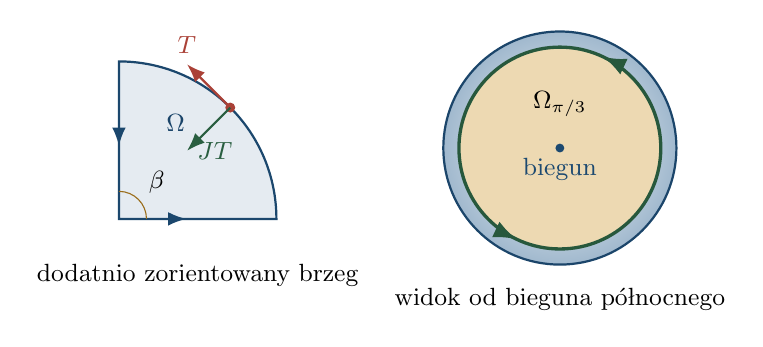
\begin{tikzpicture}[>=Latex,font=\small]
 \begin{scope}[shift={(-3,-.8)}]
  \fill[manifoldblue!12] (0,0)--(2,0) arc[start angle=0,end angle=90,radius=2]--cycle;
  \draw[manifoldblue!78!black,thick,postaction={decorate,decoration={markings,
    mark=at position .12 with {\arrow{Latex}},
    mark=at position .87 with {\arrow{Latex}}}}]
   (0,0)--(2,0) arc[start angle=0,end angle=90,radius=2]--cycle;
  \coordinate (P) at ({sqrt(2)},{sqrt(2)});
  \fill[manifoldred] (P) circle (1.8pt);
  \draw[->,manifoldred,thick] (P)--({sqrt(2)-.55},{sqrt(2)+.55})
   node[above] {$T$};
  \draw[->,manifoldgreen!75!black,thick] (P)--({sqrt(2)-.55},{sqrt(2)-.55})
   node[right] {$JT$};
  \draw[manifoldgold!75!black] (.35,0) arc[start angle=0,end angle=90,radius=.35];
  \node at (.48,.47) {$\beta$};
  \node[manifoldblue!75!black] at (.72,1.22) {$\Omega$};
  \node[below] at (1,-.45) {dodatnio zorientowany brzeg};
 \end{scope}
 \begin{scope}[shift={(2.6,.1)}]
  \shade[inner color=white,outer color=manifoldblue!43] (0,0) circle (1.48);
  \draw[manifoldblue!76!black,thick] (0,0) circle (1.48);
  \fill[manifoldgold!35] (0,0) circle ({1.48*sin(60)});
  \draw[manifoldgreen!70!black,very thick,postaction={decorate,
   decoration={markings,mark=at position .18 with {\arrow{Latex}},
   mark=at position .68 with {\arrow{Latex}}}}]
   (0,0) circle ({1.48*sin(60)});
  \fill[manifoldblue!80!black] (0,0) circle (1.6pt) node[below] {biegun};
  \node at (0,.56) {$\Omega_{\pi/3}$};
  \node[below] at (0,-1.65) {widok od bieguna północnego};
 \end{scope}
\end{tikzpicture}
\caption{Po lewej ćwierćdysk z dodatnio zorientowanym brzegiem:
$T$ jest styczny do okręgu, a $JT$ skierowany do obszaru;
zaznaczony kąt wewnętrzny to $\beta=\pi/2$.
Po prawej rzut czapki sferycznej o kącie biegunowym $\theta_0=\pi/3$.
Jej brzeg obiegamy przeciwnie do ruchu wskazówek zegara,
zgodnie z orientacją od zewnętrznej normalnej sfery.}
\label{fig:gauss-bonnet-brzeg}
\end{figure}

\begin{twierdzenie}[Gaussa--Bonneta z brzegiem i narożnikami]
\label{thm:gauss-bonnet-brzeg}
Niech $\Omega$ będzie zwartą, zorientowaną powierzchnią
riemannowską z brzegiem złożonym ze skończonej liczby
regularnych łuków klasy $C^2$. Załóżmy, że w narożnikach
istnieją jednostronne styczne i kąty wewnętrzne
$\beta_1,\ldots,\beta_m\in(0,2\pi)$. Wówczas
\begin{equation}\label{eq:gauss-bonnet-brzeg}
 \boxed{\displaystyle
 \int_\Omega K\,\dd A
 +\int_{\partial\Omega}k_g\,\dd s
 +\sum_{j=1}^m(\pi-\beta_j)
 =2\pi\chi(\Omega).}
\end{equation}
Brzeg całkujemy odcinek po odcinku. Dla brzegu gładkiego
suma po narożnikach jest pusta. Charakterystykę Eulera
można obliczyć z triangulacji:
$\chi(\Omega)=V-E+F$, gdzie $V,E,F$ są liczbami
wierzchołków, krawędzi i trójkątów; zgadza się to z
opisem homologicznym z
Twierdzenia~\ref{thm:euler-homologia}.
\end{twierdzenie}

\begin{proof}
\emph{Krok 1: forma koneksji na małym obszarze.}
Załóżmy najpierw, że $D\subset\Omega$ jest topologicznym
dyskiem, leży w jednej dodatnio zorientowanej mapie i ma
brzeg odcinkami gładki. Na otoczeniu $D$ wybierzmy
dodatnią ortonormalną ramę $(e_1,e_2)$, $e_2=Je_1$.
Istnieje ona na małym obszarze współrzędnych: wektor
pierwszej osi można unormować, a drugi otrzymać przez $J$.
Definiujemy lokalną $1$-formę
\[
 \alpha(X)=g(\nabla_Xe_1,e_2).
\]
Zgodność koneksji z metryką, czyli
$Xg(e_i,e_j)=g(\nabla_Xe_i,e_j)+g(e_i,\nabla_Xe_j)$,
daje dokładnie
\begin{equation}\label{eq:gb-rama}
 \nabla_Xe_1=\alpha(X)e_2,
 \qquad \nabla_Xe_2=-\alpha(X)e_1.
\end{equation}
Obliczmy z tego tensor krzywizny przy przyjętym tu
znaku~\eqref{eq:riemann-def}. Współczynnik przy $e_2$
wektora $\nabla_X\nabla_Ye_1$ wynosi $X(\alpha(Y))$;
wyrazy przy $e_1$ z dwóch kolejności odejmują się.
Dlatego
\[
 R(X,Y)e_1
 =\bigl(X\alpha(Y)-Y\alpha(X)-\alpha([X,Y])\bigr)e_2
 =\dd\alpha(X,Y)e_2.
\]
Dla dodatniej ramy ortonormalnej definicja krzywizny
sekcyjnej mówi, że
$g(R(e_1,e_2)e_2,e_1)=K$. Ponieważ $R(e_1,e_2)$
jest antysymetryczny względem $g$, mamy również
$g(R(e_1,e_2)e_1,e_2)=-K$. Porównanie z poprzednią
równością daje
\begin{equation}\label{eq:gb-dalpha}
 \dd\alpha=-K\,\dd A.
\end{equation}
Minus w tym miejscu jest konsekwencją naszej konwencji
dla $R$; jego zgubienie odwróciłoby znak całki z $K$.

\emph{Krok 2: krzywizna łuku jako obrót stycznej.}
Na gładkim łuku brzegu dysku można wybrać ciągłą
funkcję kąta $\vartheta(s)$ taką, że
$T=\cos\vartheta\,e_1+\sin\vartheta\,e_2$.
Różniczkując ten wzór wzdłuż łuku i podstawiając
\eqref{eq:gb-rama}, otrzymujemy
\[
 \nabla_TT
 =\bigl(\vartheta'(s)+\alpha(T)\bigr)
             (-\sin\vartheta\,e_1+\cos\vartheta\,e_2)
 =\bigl(\vartheta'(s)+\alpha(T)\bigr)JT.
\]
Stąd $k_g\,\dd s=\dd\vartheta+\alpha$ na każdym łuku.
Przy przejściu przez narożnik kierunek stycznej
obraca się dodatkowo o $\pi-\beta_j$: w wypukłym
narożniku w lewo, we wklęsłym w prawo.

Suma zmian kąta $\vartheta$ na łukach wraz z obrotami
w narożnikach wynosi $2\pi$. Jest to twierdzenie o
obrocie stycznej do dodatnio zorientowanej krzywej
Jordana na płaszczyźnie. Żeby zobaczyć, skąd bierze się
liczba $2\pi$, można łuki przybliżyć łamanymi wraz z
ich kierunkami stycznymi. W prostym wielokącie o $v$
wierzchołkach można poprowadzić $v-3$ przekątnych
i otrzymać $v-2$ trójkąty. Suma kątów wewnętrznych
to $(v-2)\pi$, a suma skrętów zewnętrznych wynosi
$v\pi-(v-2)\pi=2\pi$. Przy zagęszczaniu łamanej skręty
wewnątrz łuków dążą do całek z $\vartheta'\dd s$;
skręty w pierwotnych narożnikach zostają. Wybór
dodatniej ramki nad dyskiem nie zmienia wyniku. Przejście
od ramki współrzędnych do ramki ortonormalnej jest mapą
do $\mathrm{GL}^+(2,\R)$, a nie samym obrotem. W rozkładzie
polarnym tej macierzy dodatnio określony czynnik deformujemy
do identyczności przez $(1-s)P+s\mathrm{Id}$; niezerowa
styczna pozostaje niezerowa, więc jej liczba obrotów się
nie zmienia. Pozostaje mapa obrotów do $\mathrm{SO}(2)$.
Przedłuża się ona na cały dysk, zatem na brzegu ma stopień
zero. Liczba obrotów stycznej w naszej ramce nadal wynosi $1$.

Sumujemy równość $k_g\dd s=\dd\vartheta+\alpha$
po łukach, dodajemy obroty narożników i stosujemy
Twierdzenie Stokesa~\ref{thm:stokes-formy} oraz
\eqref{eq:gb-dalpha}:
\begin{equation}\label{eq:gb-dysk}
 \int_{\partial D}k_g\,\dd s
 +\sum_j(\pi-\beta_j)
 =2\pi+\int_{\partial D}\alpha
 =2\pi-\int_D K\,\dd A.
\end{equation}
Stokesa dla brzegu z narożnikami można tu uzyskać
z wersji dla brzegu gładkiego przez zaokrąglenie
narożników: długość usuniętych łuków i pole usuniętych
małych fragmentów dążą do zera, a $\alpha$ i $\dd\alpha$
są ograniczone na zwartym otoczeniu. Zaokrąglamy
\emph{tylko} przy zastosowaniu Stokesa; powyższe
skręty narożników pozostają w rachunku kątów.
Tak otrzymaliśmy wzór dla dysku, ponieważ $\chi(D)=1$.

\emph{Krok 3: sklejenie lokalnych wzorów.}
Wybierzmy skończoną gładką triangulację $\Omega$ na tyle
drobną, aby każdy jej trójkąt leżał w jednej mapie;
narożniki brzegu włączmy do zbioru wierzchołków.
Można to zrobić, korzystając z triangulowalności
gładkich powierzchni, z regularnymi krawędziami i
niezdegenerowanymi kątami trójkątów przy wierzchołkach. Zastosujmy~\eqref{eq:gb-dysk}
do każdego z $F$ trójkątów i zsumujmy. Całki $K$
sumują się do całki po $\Omega$. Na wewnętrznej
krawędzi dwie orientacje są przeciwne, a wraz z nimi
zmienia się znak $k_g$, więc jej wkłady znoszą się.
Zostaje całka po rzeczywistym brzegu.

Oznaczmy liczbę wierzchołków wewnętrznych przez
$V_{\mathrm w}$, a brzegowych przez $V_{\mathrm b}$.
Przy każdym wewnętrznym wierzchołku suma kątów
trójkątów wynosi $2\pi$, a przy każdym brzegowym
wynosi kąt $\beta_v$ obszaru (jeśli brzeg jest tam
gładki, $\beta_v=\pi$). Suma zewnętrznych skrętów
\emph{wszystkich trójkątów} jest więc
$3\pi F-2\pi V_{\mathrm w}-\sum_{v\in\partial\Omega}\beta_v$.
Po zsumowaniu~\eqref{eq:gb-dysk} dostajemy
\begin{equation}\label{eq:gb-liczenie}
 \int_\Omega K\,\dd A
 +\int_{\partial\Omega}k_g\,\dd s
 =-\pi F+2\pi V_{\mathrm w}
                 +\sum_{v\in\partial\Omega}\beta_v.
\end{equation}
Każda krawędź wewnętrzna należy do dwóch trójkątów,
a brzegowa do jednego. Każda składowa brzegu jest
zamkniętym cyklem z taką samą liczbą krawędzi jak
wierzchołków. Zatem
$3F=2E-V_{\mathrm b}$ (w przypadku pustego brzegu
oba ostatnie zliczenia brzegowe są zerowe).
Ponieważ $V=V_{\mathrm w}+V_{\mathrm b}$,
\[
 2\pi(V-E+F)
 -\sum_{v\in\partial\Omega}(\pi-\beta_v)
 =-\pi F+2\pi V_{\mathrm w}
                  +\sum_{v\in\partial\Omega}\beta_v.
\]
Wstawiamy tę tożsamość do~\eqref{eq:gb-liczenie}.
Sztucznie wstawione wierzchołki na gładkich częściach
brzegu mają $\beta_v=\pi$ i niczego nie dodają.
Otrzymujemy~\eqref{eq:gauss-bonnet-brzeg}.
\end{proof}

\begin{wniosek}[Gauss--Bonnet dla powierzchni zamkniętej]
\label{cor:gauss-bonnet-zamknieta}
Jeżeli $S$ jest zwartą powierzchnią bez brzegu, to
\begin{equation}\label{eq:gb-zamknieta}
 \boxed{\displaystyle\int_S K\,\dd A=2\pi\chi(S).}
\end{equation}
W szczególności dla spójnej orientowalnej powierzchni
rodzaju $g$ prawa strona wynosi $4\pi(1-g)$.
\end{wniosek}
\begin{proof}
Dla powierzchni orientowalnej stosujemy
Twierdzenie~\ref{thm:gauss-bonnet-brzeg} przy
$\partial S=\varnothing$. Z klasyfikacji powierzchni
zamkniętych $\chi(S)=2-2g$; równoważnie można tę
liczbę policzyć z dowolnej triangulacji standardowego
modelu sfery z $g$ uchwytami. Jeśli $S$ nie jest
orientowalna, bierzemy jej dwukrotne nakrycie
orientacyjne $\widetilde S\to S$. Metryka podniesiona
ma te same lokalne wartości $K$, a każdy mały obszar
na $S$ występuje dwa razy na $\widetilde S$, więc
$\int_{\widetilde S}K\dd A=2\int_SK\dd A$.
Podnosząc triangulację, otrzymujemy też
$\chi(\widetilde S)=2\chi(S)$. Dzielimy zorientowany
wzór przez $2$.
\end{proof}

\begin{przyklad}[Dysk i czapka sferyczna]
\label{prz:gb-dysk-czapka}
Dysk euklidesowy $D_r$ ma $K=0$, $k_g=1/r$ i brzeg
długości $2\pi r$. Stąd
$\int_{\partial D_r} k_g\dd s=2\pi=2\pi\chi(D_r)$.
Gdyby pominąć całkę po brzegu, wyszłaby fałszywa
równość $0=2\pi$. Dla płaskiego pierścienia o
promieniach $0<r<R$ zewnętrzny okrąg wnosi $2\pi$,
wewnętrzny $-2\pi$: suma wynosi $0$, zgodnie z
$\chi(S^1\times[0,1])=0$.

Na sferze $S_R^2$ opiszmy czapkę od bieguna północnego
do kąta biegunowego (kolatytudy) $\theta_0\in(0,\pi)$:
\[
 0\leq\theta\leq\theta_0,\qquad
 g=R^2(\dd\theta^2+\sin^2\theta\,\dd\varphi^2),
 \qquad K=R^{-2}.
\]
Z elementu pola $R^2\sin\theta\,\dd\theta\dd\varphi$
dostajemy
\[
 \int_{\Omega_{\theta_0}}K\dd A
 =\int_0^{2\pi}\int_0^{\theta_0}\sin\theta
                                     \,\dd\theta\dd\varphi
 =2\pi(1-\cos\theta_0).
\]
Brzeg ma długość $2\pi R\sin\theta_0$. Jego dodatnio
skierowany styczny to $T=(R\sin\theta_0)^{-1}
\partial_\varphi$, a $JT=-R^{-1}\partial_\theta$.
Ponieważ $\Gamma^\theta_{\varphi\varphi}
=-\sin\theta\cos\theta$, wzór~\eqref{eq:kg-def} daje
\[
 k_g=\frac{\cos\theta_0}{R\sin\theta_0},
 \qquad \int_{\partial\Omega_{\theta_0}}k_g\dd s
 =2\pi\cos\theta_0.
\]
Suma obu całek to $2\pi$, zgodnie z $\chi=1$.
Dla półsfery $\theta_0=\pi/2$ równik jest geodezyjną
i cały wkład pochodzi z $K$; dla czapki większej
niż półsfera wkład brzegu jest \emph{ujemny}.
\end{przyklad}

\begin{przyklad}[Kąty trójkąta geodezyjnego]
\label{prz:gb-trojkat}
Niech trzy łuki geodezyjne tworzą prostą zamkniętą krzywą
ograniczającą obszar $\Delta$ homeomorficzny z domkniętym
dyskiem, o kątach wewnętrznych $A,B,C$.
Wtedy $k_g=0$ na każdym boku, a $\chi(\Delta)=1$.
Z~\eqref{eq:gauss-bonnet-brzeg} wynika
\begin{equation}\label{eq:gb-trojkat}
 \int_\Delta K\,\dd A=A+B+C-\pi.
\end{equation}
W płaszczyźnie daje to $A+B+C=\pi$. Na sferze
$S_R^2$ pole trójkąta to
$R^2(A+B+C-\pi)$. Trójkąt o wierzchołkach
na biegunie północnym i w dwóch punktach równika
oddalonych o ćwierć obwodu ma $A=B=C=\pi/2$;
jako jedna ósma sfery ma pole $\pi R^2/2$.
W płaszczyźnie hiperbolicznej $K=-1$,
\[
 \operatorname{Area}(\Delta)=\pi-(A+B+C)>0.
\]
To wprost pokazuje, jak dodatnia i ujemna krzywizna
zmieniają sumę kątów.
Rysunek~\ref{fig:gb-trojkaty-modele} zestawia
odpowiednie geodezyjne w trzech modelach.
\end{przyklad}

\begin{figure}[H]
\centering
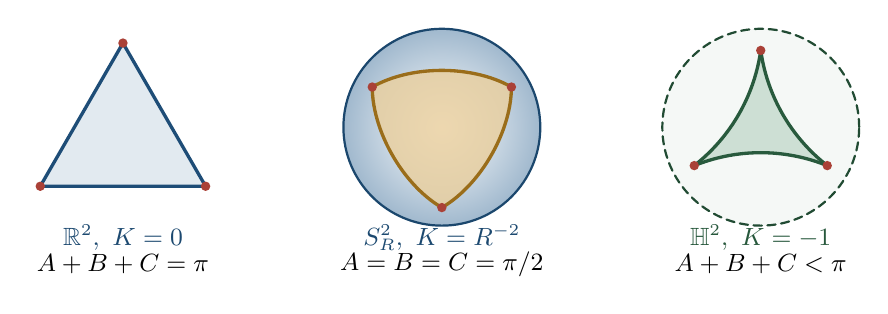
\begin{tikzpicture}[>=Latex,line cap=round,line join=round,
                     font=\small]
  % Trójkąt euklidesowy, o dokładnie równych bokach.
  \begin{scope}[shift={(-4.05,0)}]
   \fill[manifoldblue!13]
       (-1.05,-.75)--(1.05,-.75)--(0,1.06865)--cycle;
   \draw[manifoldblue!85!black,very thick]
       (-1.05,-.75)--(1.05,-.75)--(0,1.06865)--cycle;
   \foreach \x/\y in {-1.05/-.75,1.05/-.75,0/1.06865}
      \fill[manifoldred] (\x,\y) circle (1.7pt);
   \node[manifoldblue!80!black] at (0,-1.40) {$\R^2,\ K=0$};
   \node at (0,-1.74) {$A+B+C=\pi$};
  \end{scope}
  % Oktant sferyczny widziany w rzucie prostopadłym z (1,1,1).
  \begin{scope}
   \shade[inner color=white,outer color=manifoldblue!43] (0,0) circle (1.25);
   \draw[manifoldblue!78!black,thick] (0,0) circle (1.25);
   \path[fill=manifoldgold!43,opacity=.83]
     plot[domain=0:90,samples=30]
       ({1.25*(cos(\x)-sin(\x))/sqrt(2)},
        {1.25*(cos(\x)+sin(\x))/sqrt(6)}) --
     plot[domain=0:90,samples=30]
       ({-1.25*cos(\x)/sqrt(2)},
        {1.25*(cos(\x)-2*sin(\x))/sqrt(6)}) --
     plot[domain=0:90,samples=30]
       ({1.25*sin(\x)/sqrt(2)},
        {1.25*(-2*cos(\x)+sin(\x))/sqrt(6)}) -- cycle;
   \draw[manifoldgold!75!black,very thick]
     plot[domain=0:90,samples=30]
       ({1.25*(cos(\x)-sin(\x))/sqrt(2)},
        {1.25*(cos(\x)+sin(\x))/sqrt(6)});
   \draw[manifoldgold!75!black,very thick]
     plot[domain=0:90,samples=30]
       ({-1.25*cos(\x)/sqrt(2)},
        {1.25*(cos(\x)-2*sin(\x))/sqrt(6)});
   \draw[manifoldgold!75!black,very thick]
     plot[domain=0:90,samples=30]
       ({1.25*sin(\x)/sqrt(2)},
        {1.25*(-2*cos(\x)+sin(\x))/sqrt(6)});
   \foreach \x/\y in {.88388/.51031,-.88388/.51031,0/-1.02062}
      \fill[manifoldred] (\x,\y) circle (1.7pt);
   \node[manifoldblue!80!black] at (0,-1.40) {$S_R^2,\ K=R^{-2}$};
   \node at (0,-1.74) {$A=B=C=\pi/2$};
  \end{scope}
  % Poincaré: boki są łukami okręgów prostopadłych do brzegu.
  \begin{scope}[shift={(4.05,0)}]
   \pgfmathsetmacro{\hc}{(1+.78^2)/.78}
   \pgfmathsetmacro{\hr}{sqrt(\hc^2-1)}
   \pgfmathsetmacro{\ha}{asin(.78*sin(60)/\hr)}
   \fill[manifoldgreen!5] (0,0) circle (1.25);
   \draw[manifoldgreen!60!black,densely dashed,thick]
        (0,0) circle (1.25);
   \path[fill=manifoldgreen!25]
    plot[domain=\ha:-\ha,samples=30]
      ({1.25*(\hc*cos(150)+\hr*cos(330+\x))},
       {1.25*(\hc*sin(150)+\hr*sin(330+\x))}) --
    plot[domain=\ha:-\ha,samples=30]
      ({1.25*(\hc*cos(270)+\hr*cos(450+\x))},
       {1.25*(\hc*sin(270)+\hr*sin(450+\x))}) --
    plot[domain=\ha:-\ha,samples=30]
      ({1.25*(\hc*cos(390)+\hr*cos(570+\x))},
       {1.25*(\hc*sin(390)+\hr*sin(570+\x))}) -- cycle;
   \foreach \m in {150,270,390}
     \draw[manifoldgreen!72!black,very thick]
       plot[domain=\ha:-\ha,samples=35]
       ({1.25*(\hc*cos(\m)+\hr*cos(\m+180+\x))},
        {1.25*(\hc*sin(\m)+\hr*sin(\m+180+\x))});
   \foreach \ang in {90,210,330}
     \fill[manifoldred] (\ang:.975) circle (1.7pt);
   \node[manifoldgreen!70!black] at (0,-1.40) {$\mathbb H^2,\ K=-1$};
   \node at (0,-1.74) {$A+B+C<\pi$};
  \end{scope}
\end{tikzpicture}
\caption{Trójkąty geodezyjne w geometrii euklidesowej,
na sferze i w modelu dyskowym płaszczyzny hiperbolicznej.
Środkowy trójkąt jest oktantem sfery: każdy jego bok
stanowi ćwiartkę wielkiego koła, a każdy kąt jest prosty.
W dysku boki leżą na okręgach prostopadłych do
przerywanego brzegu, który nie należy do $\mathbb H^2$.
Znaki $K$ odpowiadają sumom kątów ze wzoru
\eqref{eq:gb-trojkat}.}
\label{fig:gb-trojkaty-modele}
\end{figure}

\begin{przyklad}[Sfera i torus: całka nie zależy od metryki]
\label{prz:gb-sfera-torus}
Na sferze $S_R^2$ stała krzywizna $R^{-2}$ i pole
$4\pi R^2$ dają całkę $4\pi$; promień się skraca.
Na torusie obrotowym niech $a>b>0$, a parametryzacja
ma postać
\[
 X(u,v)=((a+b\cos v)\cos u,
          (a+b\cos v)\sin u,b\sin v),
 \qquad (u,v)\in[0,2\pi]^2.
\]
Różniczkując $X$ znajdujemy
$g=(a+b\cos v)^2\dd u^2+b^2\dd v^2$ i
$\dd A=b(a+b\cos v)\dd u\dd v$.
Dla metryki postaci $\dd s^2+f(s)^2\dd u^2$
rachunek z symboli Christoffela daje
$K=-f''(s)/f(s)$: jedyne niezerowe symbole to
$\Gamma^s_{uu}=-ff'$ oraz
$\Gamma^u_{su}=\Gamma^u_{us}=f'/f$, więc
$g(R(\partial_s,\partial_u)\partial_u,\partial_s)
=-ff''$, a mianownik we wzorze na $K$ wynosi $f^2$.
Biorąc $s=bv$ i $f(s)=a+b\cos(s/b)$, otrzymujemy
\[
 K(u,v)=\frac{\cos v}{b(a+b\cos v)},\qquad
 \int_{T^2}K\dd A
 =\int_0^{2\pi}\!\int_0^{2\pi}\cos v\,\dd u\dd v=0.
\]
Krzywizna dodatnia po zewnętrznej i ujemna po
wewnętrznej stronie torusa znoszą się w całce.
Zgadza się to z $\chi(T^2)=0$. Zmiana metryki
zmienia lokalne $K$ i $\dd A$, ale nie może zmienić
ich całki na tej samej zwartej powierzchni.
\end{przyklad}

\subsection*{Uogólnienie I: krzywizna skupiona w punktach}

Na gładkiej powierzchni krzywizna $K\,\dd A$ jest
rozłożona na obszarze. Można jednak skleić płaskie
wielokąty w zamkniętą powierzchnię: wnętrze każdej ściany
i punkt wewnętrzny każdej sklejonej krawędzi ma płaskie
otoczenie. Cała krzywizna jest wtedy skupiona w
\emph{wierzchołkach}. Przy wierzchołku $v$ sumujemy kąty
przylegających ścian i oznaczamy tę sumę przez $\theta_v$.
Brakujący względem pełnego obrotu kąt
\begin{equation}\label{eq:gb-deficyt-kata}
 \delta_v=2\pi-\theta_v
\end{equation}
nazywamy \emph{deficytem kąta}. Może być ujemny, jeśli
wokół wierzchołka mieści się więcej niż $2\pi$.
Lokalnie jest to powierzchnia stożka o kącie całkowitym
$\theta_v$; zwykły płaski punkt ma $\theta_v=2\pi$.

\begin{twierdzenie}[Wielościenna postać Gaussa--Bonneta]
\label{thm:gb-wielosciany}
Niech $P$ będzie zwartą powierzchnią bez brzegu,
powstałą przez sklejenie skończonej liczby trójkątów
euklidesowych wzdłuż całych boków. Oznaczmy zbiór
jej wierzchołków przez $\mathrm{Vert}(P)$. Wówczas
\begin{equation}\label{eq:gb-wielosciany}
 \boxed{\displaystyle\sum_{v\in\mathrm{Vert}(P)}(2\pi-\theta_v)
                      =2\pi\chi(P).}
\end{equation}
W sumie można pominąć wierzchołki o $\theta_v=2\pi$.
\end{twierdzenie}
\begin{proof}
Niech $V,E,F$ oznaczają liczbę wierzchołków, krawędzi
i trójkątów. Przy każdym $v$ odejmujemy od $2\pi$
wszystkie kąty trójkątów stykających się w $v$.
Każdy kąt pojawia się dokładnie raz, a suma trzech kątów
jednego płaskiego trójkąta wynosi $\pi$. Dlatego
\[
 \sum_v(2\pi-\theta_v)=2\pi V-\pi F.
\]
Każdy trójkąt ma trzy boki, a każda krawędź należy do
dwóch trójkątów, zatem $3F=2E$. W konsekwencji
$2\pi V-\pi F=2\pi(V-E+F)=2\pi\chi(P)$.
Ten rachunek wyjaśnia, dlaczego liczymy kąty \emph{wewnątrz}
ścian, a nie kąty dwuścienne bryły w $\R^3$.
\end{proof}

\begin{przyklad}[Czworościan i sześcian]
W każdym wierzchołku foremnego czworościanu spotykają
się trzy trójkąty równoboczne. Zatem $\theta_v=\pi$,
$\delta_v=\pi$, a cztery wierzchołki dają $4\pi$.
W sześcianie spotykają się trzy kąty proste:
$\theta_v=3\pi/2$ i $\delta_v=\pi/2$; osiem
wierzchołków znowu daje $4\pi$. Obie powierzchnie są
topologicznie sferami, więc $2\pi\chi(S^2)=4\pi$.
Rozkład krzywizny jest inny, lecz suma pozostaje taka sama.
\end{przyklad}

Możemy połączyć krzywiznę gładką z punktowymi deficytami.
Załóżmy, że zwarta powierzchnia $S$ bez brzegu ma skończenie wiele
punktów $p_i$ o otoczeniach będących płaskimi stożkami
o kątach $\theta_i$, a poza nimi jest gładką powierzchnią
riemannowską. Wtedy
\begin{equation}\label{eq:gb-stozki}
 \boxed{\displaystyle
 \int_{S\setminus\{p_1,\ldots,p_N\}}K\,\dd A
       +\sum_{i=1}^N(2\pi-\theta_i)
       =2\pi\chi(S).}
\end{equation}
Istotnie, wytnijmy mały dysk stożkowy przy każdym $p_i$.
Otrzymana gładka powierzchnia ma charakterystykę Eulera
$\chi(S)-N$. Brzeg usuniętego dysku ma długość
$\theta_i r$ i krzywiznę geodezyjną $-1/r$:
minus bierze się z orientacji brzegu \emph{dziury}.
Jego wkład do całki brzegowej to zatem $-\theta_i$.
Podstawienie do~\eqref{eq:gauss-bonnet-brzeg} daje
$\int K\,\dd A-\sum_i\theta_i=2\pi(\chi(S)-N)$,
co po przeniesieniu wyrazów jest~\eqref{eq:gb-stozki}.
Dla powierzchni nieorientowalnej stosujemy ten rachunek
na dwukrotnym nakryciu orientacyjnym i dzielimy przez $2$:
całka, liczba deficytów i charakterystyka Eulera podwajają się.
Gdy część gładka jest płaska, pozostaje dokładnie
\eqref{eq:gb-wielosciany}. W języku miar można myśleć
o krzywiźnie jako o $K\,\dd A+\sum_i\delta_i\delta_{p_i}$:
symbol $\delta_{p_i}$ oznacza masę jednostkową w punkcie,
a współczynnik $\delta_i$ jest deficytem kąta.

\subsection*{Uogólnienie II: parzysty wymiar i twierdzenie Cherna}

W wymiarze dwa $K$ jest całą informacją o krzywiźnie
riemannowskiej w danym punkcie. W wymiarze cztery lub
większym nie wystarczy scałkować samej krzywizny skalarnej:
liczy się określona \emph{kombinacja} składowych tensora
Riemanna. Oto jej precyzyjny opis w języku form.

Niech $(M^{2m},g)$, $m\geq1$, będzie zorientowaną rozmaitością
riemannowską, a $(e_1,\ldots,e_{2m})$ dodatnio zorientowaną
lokalną ramą ortonormalną. Macierz form krzywizny ma wyrazy
\[
 \Omega_{ij}(X,Y)=g(R(X,Y)e_j,e_i),\qquad
 \Omega_{ji}=-\Omega_{ij}.
\]
\emph{Pfaffian} takiej macierzy jest formą stopnia $2m$:
\begin{equation}\label{eq:gb-pfaff-def}
 \operatorname{Pf}(\Omega)=\frac1{2^m m!}
 \sum_{\sigma\in S_{2m}}\operatorname{sgn}(\sigma)
 \Omega_{\sigma(1)\sigma(2)}\wedge\cdots\wedge
 \Omega_{\sigma(2m-1)\sigma(2m)}.
\end{equation}
Zasada konstrukcji: parujemy wszystkie kierunki styczne,
bierzemy iloczyny zewnętrzne odpowiadających im krzywizn
i dodajemy je ze znakami wyznaczonymi przez permutacje.
Dlaczego otrzymujemy globalną formę? Przy zmianie dodatniej
ramki macierzą $Q\in\mathrm{SO}(2m)$ mamy
$\widetilde\Omega=Q^{\mathsf T}\Omega Q$ oraz
$\operatorname{Pf}(Q^{\mathsf T}\Omega Q)
=\det(Q)\operatorname{Pf}(\Omega)=\operatorname{Pf}(\Omega)$.
Tożsamość wynika z rozpisania wzoru permutacyjnego:
po antysymetryzacji iloczyn $2m$ współczynników $Q$
daje jego wyznacznik. Nie ma pochodnych $Q$, bo
$\Omega$ pochodzi z tensora krzywizny. Lokalne formy
sklejają się więc na przecięciach map.
W orientacji przeciwnej znak formy się zmienia razem
ze znakiem całkowania. Dla $m=1$ dostajemy po prostu
$\operatorname{Pf}(\Omega)=\Omega_{12}=K\,\dd A$;
normalizacja z poniższego twierdzenia daje zatem
dokładnie~\eqref{eq:gb-zamknieta}.

\begin{twierdzenie}[Cherna--Gaussa--Bonneta]
\label{thm:chern-gauss-bonnet}
Jeżeli $(M^{2m},g)$ jest zwartą, zorientowaną
rozmaitością riemannowską \emph{bez brzegu}, to
\begin{equation}\label{eq:chern-gauss-bonnet}
 \boxed{\displaystyle
 \chi(M)=\frac1{(2\pi)^m}\int_M
                       \operatorname{Pf}(\Omega).}
\end{equation}
Forma $\operatorname{Pf}(\Omega)/(2\pi)^m$ reprezentuje
w kohomologiach de Rhama rzeczywistą \emph{klasę Eulera}
wiązki stycznej $TM$. Całka nie zależy więc od wyboru
metryki, choć sam Pfaffian zależy od niej punktowo.
\end{twierdzenie}

Dowód przez teorię Cherna--Weila przedstawiamy w
Rozdziale~\ref{ch:chern-weil}. Warto rozdzielić jego kroki:
zamkniętość formy i niezależność jej klasy od koneksji
nie wystarczają jeszcze do rozpoznania klasy Eulera.
Tę identyfikację daje Stwierdzenie~\ref{prop:euler-identification-26},
korzystające z klasy Thoma z Twierdzenia~\ref{thm:euler-thom-16}.
Lemat~\ref{lem:angular-form-26} ustala normalizację formy kątowej:
jej całka po każdym włóknie sferycznym wynosi $1$.
Twierdzenie Stokesa wiąże następnie całkę z Pfaffianu
z sumą indeksów zer pola stycznego, równą $\chi(M)$.
Tu wykonujemy dwa testy wzoru: przypadek $m=1$ powyżej
oraz następujący przykład czterowymiarowy.

W wymiarze cztery
\begin{equation}\label{eq:gb-pfaff-4}
 \operatorname{Pf}(\Omega)=
 \Omega_{12}\wedge\Omega_{34}
 -\Omega_{13}\wedge\Omega_{24}
 +\Omega_{14}\wedge\Omega_{23}.
\end{equation}
Po rozpisaniu w ortonormalnej ramie, przy normach
$|\mathrm{Rm}|^2=\sum_{i,j,k,l}R_{ijkl}^2$ i
$|\mathrm{Ric}|^2=\sum_{i,j}\mathrm{Ric}_{ij}^2$,
otrzymujemy równoważną postać. Wskażmy algebraiczny krok
prowadzący do współczynników $1,-4,1$. Niech $\eta^a$
będzie ramką dualną i $\varepsilon_{1234}=1$ symbolem
całkowicie antysymetrycznym. Ponieważ
$\Omega_{ij}=\frac12\mathcal R_{abji}\eta^a\wedge\eta^b$,
wzór permutacyjny daje
\[
 \operatorname{Pf}(\Omega)
 =\frac1{32}\varepsilon_{ijkl}\varepsilon_{abcd}
       \mathcal R_{abji}\mathcal R_{cdlk}\,\dd\mu_g
 =\frac18\bigl(|\mathrm{Rm}|^2-4|\mathrm{Ric}|^2
                         +\mathrm{Scal}^2\bigr)\,\dd\mu_g.
\]
W ostatnim przejściu rozwijamy
$\varepsilon_{ijkl}\varepsilon_{abcd}
=\det(\delta_{u v})_{u\in(i,j,k,l),\,v\in(a,b,c,d)}$.
Po zebraniu 24 permutacji, użyciu antysymetrii par,
symetrii zamiany par i pierwszej tożsamości Bianchiego
kontrakcja wynosi
$4|\mathrm{Rm}|^2-16|\mathrm{Ric}|^2+4\mathrm{Scal}^2$.
Iloczyn czynnika $1/8$ z $(2\pi)^{-2}$ daje zatem
\begin{equation}\label{eq:gb-4d}
 \chi(M^4)=\frac1{32\pi^2}\int_{M^4}
 \bigl(|\mathrm{Rm}|^2-4|\mathrm{Ric}|^2
                    +\mathrm{Scal}^2\bigr)\,\dd\mu_g.
\end{equation}
Obecność trzech składników pokazuje, czemu
$\int\mathrm{Scal}\,\dd\mu_g$ sama nie może być
czterowymiarowym odpowiednikiem $\int K\,\dd A$.

\begin{przyklad}[Iloczyn dwóch sfer]
Na $M=S_a^2\times S_b^2$ wybierzmy ramę $(e_1,e_2)$
styczną do pierwszej sfery i $(e_3,e_4)$ styczną do
drugiej. W metryce iloczynowej jedyne niezerowe formy
krzywizny występujące w~\eqref{eq:gb-pfaff-4} to
$\Omega_{12}=a^{-2}\dd A_a$ i
$\Omega_{34}=b^{-2}\dd A_b$. Stąd
\[
 \frac1{(2\pi)^2}\int_M\operatorname{Pf}(\Omega)
 =\frac1{4\pi^2}
   \left(\frac{4\pi a^2}{a^2}\right)
   \left(\frac{4\pi b^2}{b^2}\right)=4.
\]
Zgadza się to z $\chi(S^2\times S^2)=4$:
komórki iloczynowego rozkładu CW to jedna $0$-komórka,
dwie $2$-komórki i jedna $4$-komórka. Promienie ponownie
znikają z wyniku.
\end{przyklad}

\subsection*{Brzeg, niezwartość i nieparzysty wymiar}

Dla zwartej, zorientowanej rozmaitości riemannowskiej
parzystego wymiaru o gładkim brzegu twierdzenie Cherna
ma wersję z poprawką brzegową. Jej precyzyjną definicję
i dowód podajemy w
Twierdzeniu~\ref{thm:CGB-boundary-26}; tutaj zapisujemy wzór:
\begin{equation}\label{eq:chern-gb-brzeg-idea}
 \chi(M^{2m})=
 \frac1{(2\pi)^m}\int_M\operatorname{Pf}(\Omega)
 +\int_{\partial M}\mathcal B_g.
\end{equation}
Forma $\mathcal B_g$ na gładkim brzegu zawiera jego
geometrię wewnętrzną i sposób zanurzenia w $M$
(drugą formę fundamentalną). Nie jest w ogólności
samą krzywizną Gaussa brzegu. W wymiarze dwa mamy
$\mathcal B_g=k_g\,\dd s/(2\pi)$; dla brzegu
z narożnikami dochodzą jeszcze skręty opisane
w~\eqref{eq:gauss-bonnet-brzeg}. Zasadniczy test:
domknięta płaska kula $\overline B^{2m}\subset\R^{2m}$
ma zerowy Pfaffian we wnętrzu, lecz $\chi(\overline B^{2m})=1$,
zatem cały wkład w~\eqref{eq:chern-gb-brzeg-idea}
pochodzi z $\partial\overline B^{2m}$.

Bez zwartości całka po wnętrzu również nie musi
odtwarzać $\chi$: dla całej płaskiej $\R^2$
mamy $\int_{\R^2}K\,\dd A=0$ i $\chi(\R^2)=1$.
Na wyczerpujących ją dyskach $B_R$ brakujący wkład
jest widoczny jako $\int_{\partial B_R}k_g\,\dd s=2\pi$.
W twierdzeniach dla przestrzeni niezwartych trzeba
kontrolować granicę takiego wyrazu przy $R\to\infty$;
nie wolno go po prostu skreślić.

Dla porównania, każda zwarta orientowalna rozmaitość
\emph{bez brzegu} nieparzystego wymiaru ma $\chi(M)=0$.
Wynika to z dualności Poincarégo nad $\Q$:
$b_i=b_{n-i}$, a gdy $n$ jest nieparzyste,
składniki $(-1)^i b_i$ i $(-1)^{n-i}b_{n-i}$
w sumie Eulera znoszą się parami. Nie ma więc
w nieparzystym wymiarze analogicznej nietrywialnej
całki z Pfaffianu stopnia najwyższego.

\begin{uwaga}[Co mówi, a czego nie mówi całkowita krzywizna?]
Dla zamkniętej powierzchni orientowalnej rodzaju $g=0$
całka $K$ jest dodatnia, dla $g=1$ zerowa, a dla
$g\geq2$ ujemna. Nie wynika stąd, że $K$ ma ten sam
znak w każdym punkcie: wzór określa sumę wkładów.
Wzór z samym $K$ jest \emph{dwuwymiarowy};
uogólnienie Cherna dotyczy zwartych rozmaitości
riemannowskich parzystego wymiaru. Nie stosujemy
żadnego z tych zapisów bezpośrednio do niezwartych
czterowymiarowych metryk \emph{lorentzowskich}
Schwarzschilda i Kerra: potrzebne są inne założenia,
odpowiednia wersja dla sygnatury metryki i analiza brzegu
bądź zachowania w nieskończoności.
\end{uwaga}

\par\smallskip
{\footnotesize\noindent\emph{Dalsza lektura:}
\href{https://www.wim.uni-mannheim.de/media/Lehrstuehle/wim/schmidt/FSS2024/Riemannian_Geometry/Web/RGch5.html}{krzywizna},
\href{https://davidtong.org/pdfs/teaching/general-relativity/gr6.pdf}{Schwarzschild i Kerr},
\href{https://arxiv.org/pdf/2412.04135}{rozwiązania typu Kerra w teorii DHOST},
\href{https://math.stanford.edu/~ralph/math215b/Milnor.pdf}{Milnor},
\href{https://web.math.utk.edu/~langford/RG.pdf}{porównania},
\href{https://math.mit.edu/~lurie/papers/hadamard.pdf}{Cartan--Hadamard},
\href{https://math.mit.edu/~lguth/Exposition/systmet.pdf}{skalar i małe kule},
\href{https://www.math.uchicago.edu/~may/REU2022/REUPapers/Hale.pdf}{Gauss--Bonnet},
\href{https://arxiv.org/pdf/1111.4972}{Cherna--Gaussa--Bonneta},
\href{https://pages.uoregon.edu/gilkey/P251-Gauss-Bonnet-v7a.pdf}{uogólnienie z brzegiem}.\par}


\part{Grupy Liego i geometria globalna}
\chapter{Grupy Liego i ich algebry}
\label{ch:grupy-liego}
\index{grupa Liego}
\index{algebra Liego}

W Rozdziale~\ref{ch:rozmaitosci} grupa ortogonalna pojawiła się jako
rozmaitość, a w Rozdziale~\ref{ch:pola} poznaliśmy przepływy i nawias pól.
Teraz połączymy te konstrukcje. W grupie Liego każdy wektor styczny
przy elemencie neutralnym wyznacza pole na całej grupie, a przepływ
tego pola daje rodzinę symetrii zależną od jednego parametru.
Grupy i homomorfizmy wystąpiły już w
Definicji~\ref{def:grupa-hom-5}; tutaj wymagamy ponadto gładkości.

\section{Grupa z gładką strukturą}
\label{sec:grupy-liego-przyklady}

\begin{definicja}[Grupa Liego]
\label{def:grupa-liego}
\index{grupa Liego!definicja}
\emph{Grupą Liego} nazywamy skończenie wymiarową gładką rozmaitość
bez brzegu $G$, wyposażoną w strukturę grupy, dla której
\[
 m:G\times G\longrightarrow G,\quad m(g,h)=gh,
 \qquad \iota:G\longrightarrow G,\quad\iota(g)=g^{-1}
\]
są gładkie. Jej element neutralny oznaczamy $e$.
Intuicyjnie można w niej wykonywać działania grupowe i jednocześnie
różniczkować je względem parametrów. Homomorfizm grup Liego nazywamy
\emph{gładkim}, gdy jest gładki jako odwzorowanie rozmaitości.
\end{definicja}

Dla $g\in G$ oznaczamy przez $L_g(h)=gh$ i $R_g(h)=hg$
translacje. Obie są dyfeomorfizmami: są gładkie jako ograniczenia
$m$, a ich odwrotnościami są odpowiednio $L_{g^{-1}}$ i
$R_{g^{-1}}$. Pozwalają przenosić rachunek z punktu $e$ do
każdego punktu grupy.

\begin{przyklad}[Grupy macierzy odwracalnych]
\label{prz:gl-liego}
\index{grupa ogólna liniowa}
Grupa $\mathrm{GL}(n,\R)$ z
Dodatku~\ref{sec:app-grupa-gl} jest otwartym podzbiorem
$\R^{n^2}$, bo wyznacznik jest wielomianem.
Iloczyn macierzy jest wielomianowy w ich współczynnikach, a
\[
 A^{-1}=\frac{\operatorname{adj}A}{\det A}
\]
jest gładki na tym otwartym zbiorze. Stąd $\mathrm{GL}(n,\R)$
jest grupą Liego wymiaru $n^2$. Ten sam argument, po potraktowaniu
części rzeczywistych i urojonych współczynników jako współrzędnych,
daje $\mathrm{GL}(n,\C)$ wymiaru rzeczywistego $2n^2$.
W obu przypadkach, dla $\mathbb K\in\{\R,\C\}$,
$T_I\mathrm{GL}(n,\mathbb K)=M_n(\mathbb K)$
jako przestrzeń rzeczywista: otwarty podzbiór przestrzeni macierzy
ma tę samą przestrzeń styczną co otoczenie.
\end{przyklad}

\begin{przyklad}[Grupy ortogonalne]
\label{prz:orth-liego}
\index{grupa ortogonalna}
W Przykładzie o grupie ortogonalnej w
Rozdziale~\ref{ch:rozmaitosci} wykazaliśmy, że
grupa $\mathrm O(n)$ z Dodatku~\ref{sec:app-grupa-o}
jest gładką rozmaitością i że
$T_I\mathrm O(n)=\{X:X^T=-X\}$. Mnożenie jest ograniczeniem
wielomianowego mnożenia macierzy, a odwrotność ma tutaj prostą
postać $A^{-1}=A^T$, więc oba działania są gładkie.
Ponieważ $\det A\in\{-1,1\}$ na $\mathrm O(n)$,
$\mathrm{SO}(n)$ jest
otwartą i domkniętą podrozmaitością $\mathrm O(n)$.
Jest podgrupą Liego tego samego wymiaru $n(n-1)/2$.
Jej przestrzeń styczna przy $I$ również składa się z
macierzy skośnie symetrycznych.
\end{przyklad}

\begin{przyklad}[Torus jako grupa]
\label{prz:torus-liego}
\index{torus!jako grupa Liego}
Na torusie $T^k=\R^k/\Z^k$ z Przykładu~\ref{prz:torus}
kładziemy $[x]+[y]=[x+y]$ i $-[x]=[-x]$. W lokalnych mapach
utworzonych z rzutowania $\R^k\to T^k$ działania mają postać
zwykłego dodawania i zmiany znaku, z ewentualną całkowitą
translacją współrzędnych. Są więc gładkie. Równoważny model
\[
 T^k\longrightarrow(S^1)^k,\qquad
 [x_1,\ldots,x_k]\longmapsto
 (e^{2\pi i x_1},\ldots,e^{2\pi i x_k})
\]
przekształca dodawanie w mnożenie zespolone na każdej współrzędnej;
odwrotność staje się sprzężeniem zespolonym. Dla $k=2$ wzór
$(u,v)\mapsto((R+r\cos v)\cos u,(R+r\cos v)\sin u,r\sin v)$,
gdzie $R>r>0$, wyznacza dyfeomorfizm
$(\R/2\pi\Z)^2$ na torus obrotowy z
Rozdziału~\ref{ch:rozmaitosci}. Przenosi on na ten torus
strukturę grupy. Jego mnożenie zależy od tej identyfikacji, a nie
od dodawania punktów w otaczającej go przestrzeni $\R^3$.
\end{przyklad}

\begin{przyklad}[Macierze specjalnie unitarne]
\label{prz:su2-liego}
\index{grupa specjalna unitarna}
Niech $\mathrm{SU}(2)$ będzie grupą z
Dodatku~\ref{sec:app-grupa-u}.
Z warunków $U^{-1}=U^*$ i $\det U=1$ wynika, przez porównanie
wzorów na odwrotność, że każdy jej element ma jedyną postać
\begin{equation}\label{eq:su2-macierz}
 U(a,b)=\begin{pmatrix}a&b\\-\bar b&\bar a\end{pmatrix},
 \qquad |a|^2+|b|^2=1.
\end{equation}
Odwrotnie, bezpośrednie pomnożenie pokazuje
$U(a,b)^*U(a,b)=I$ i $\det U(a,b)=|a|^2+|b|^2=1$.
Współrzędne $(\Re a,\Im a,\Re b,\Im b)$ identyfikują zatem
$\mathrm{SU}(2)$ gładko ze sferą $S^3\subset\R^4$.
Mnożenie macierzy ogranicza się do gładkiego odwzorowania
$S^3\times S^3\to S^3$, a odwrotność $U^{-1}=U^*$ jest
ograniczeniem rzeczywiście liniowego odwzorowania na $M_2(\C)$.
Jest to więc zwarta, trójwymiarowa grupa Liego.
\end{przyklad}

\section{Od wektora przy jedności do algebry Liego}
\label{sec:algebra-liego}

\begin{definicja}[Pole lewostronnie niezmiennicze i algebra Liego]
\label{def:algebra-liego}
\index{pole lewostronnie niezmiennicze}
\index{algebra Liego!definicja}
Pole $V$ na $G$ jest \emph{lewostronnie niezmiennicze}, gdy
$(L_g)_*V=V$ dla każdego $g\in G$. Dla $X\in T_eG$ oznaczamy
\[
 X^L_g:=(\dd L_g)_eX.
\]
\emph{Algebrą Liego} grupy $G$ nazywamy przestrzeń
$\mathfrak g=T_eG$ z nawiasem
\[
 [X,Y]_{\mathfrak g}:=[X^L,Y^L]_e.
\]
Wektor przy jedności opisuje ruch nieskończenie mały; translacje
przenoszą ten sam ruch do wszystkich punktów. Przykładami są
$\mathfrak{gl}(n,\R)=M_n(\R)$ i, jak pokażemy niżej,
$\mathfrak t^k\cong\R^k$ z zerowym nawiasem.
\end{definicja}

\begin{twierdzenie}[Niezmienniczość i zamknięcie na nawias]
\label{thm:lie-algebra-fields}
Odwzorowanie $X\mapsto X^L$ jest izomorfizmem liniowym
$T_eG$ na przestrzeń pól lewostronnie niezmienniczych.
Nawias dwóch takich pól jest znowu lewostronnie niezmienniczy.
W szczególności $\mathfrak g$ jest algebrą Liego: jej nawias jest
dwuliniowy, antysymetryczny i spełnia tożsamość Jacobiego.
\end{twierdzenie}
\begin{proof}
Gładkość $X^L$ wynika z gładkości różniczki mnożenia po
ograniczeniu do $G\times\{e\}$. Dla $g,h\in G$ mamy
$L_g\circ L_h=L_{gh}$, więc reguła łańcucha daje
\[
 (\dd L_g)_h X^L_h
 = (\dd L_g)_h(\dd L_h)_eX
 = (\dd L_{gh})_eX=X^L_{gh}.
\]
Jest to niezmienniczość. Jeśli $V$ jest dowolnym polem
lewostronnie niezmienniczym, to po podstawieniu $h=e$
otrzymujemy $V_g=(\dd L_g)_eV_e$; zatem $V=(V_e)^L$.
Wartość przy $e$ jest więc odwrotnością odwzorowania
$X\mapsto X^L$, a oba odwzorowania są liniowe.

Dla dyfeomorfizmu $F$ zachodzi
$F_*[V,W]=[F_*V,F_*W]$. Można to sprawdzić bezpośrednio
na funkcji $f$: definicja pola przeniesionego daje
$(F_*V)(f)=(V(f\circ F))\circ F^{-1}$, a po dwukrotnym
zastosowaniu tego wzoru różnica złożeń staje się
$([V,W](f\circ F))\circ F^{-1}$.
Stosując tę równość do $F=L_g$ i $V=X^L$, $W=Y^L$,
dostajemy
\[
 (L_g)_*[X^L,Y^L]
 =[(L_g)_*X^L,(L_g)_*Y^L]=[X^L,Y^L].
\]
Własności nawiasu pól zostały dowiedzione w
Fakcie~\ref{fakt:nawias-wlasnosci}. Przez izomorfizm
$X\mapsto X^L$ przechodzą na nawias w $T_eG$.
\end{proof}

\begin{przyklad}[Komutator macierzy]
\label{prz:lie-bracket-matrix}
\index{komutator macierzy}
Na otwartym $\mathrm{GL}(n,\R)$ pole odpowiadające macierzy
$X$ ma wartość $X^L_A=AX$. Dla $Y^L_A=AY$ różniczka
odwzorowania $A\mapsto AY$ w kierunku $H$ jest równa $HY$.
Wzór współrzędny na nawias z~\eqref{eq:nawias-wspolrzedne}
daje więc
\[
 [X^L,Y^L]_A
 =\D(Y^L)_A[AX]-\D(X^L)_A[AY]
 =AXY-AYX=A(XY-YX).
\]
Stąd $[X,Y]_{\mathfrak{gl}}=XY-YX$. To samo obliczenie,
po ograniczeniu pól stycznych do podgrupy macierzy, obowiązuje
dla $\mathrm O(n)$, $\mathrm{SO}(n)$ i $\mathrm{SU}(2)$.
W szczególności
$\mathfrak{so}(n)=\{X:X^T=-X\}$ jest zamknięta na komutator,
bo $(XY-YX)^T=-(XY-YX)$.

Dla $\mathrm{SU}(2)$ różniczkowanie $U^*U=I$ i $\det U=1$
w punkcie $I$ daje odpowiednio $X^*+X=0$ i
$\operatorname{tr}X=0$; różniczka wyznacznika w kierunku
$X$ wynosi $\operatorname{tr}X$, co widać z rozwinięcia
$\det(I+tX)=1+t\operatorname{tr}X+t^2\det X$.
Ponieważ obie strony mają wymiar
rzeczywisty trzy, otrzymujemy
\[
 \mathfrak{su}(2)
 =\left\{\begin{pmatrix}i\alpha&z\\-\bar z&-i\alpha\end{pmatrix}
 :\alpha\in\R,\ z\in\C\right\}.
\]
Na torusie translacje w mapach ilorazowych mają stałą
różniczkę równą identyczności. Odpowiadające im pola mają
stałe współczynniki, więc ich nawias znika:
$\mathfrak t^k\cong(\R^k,0)$.
\end{przyklad}

\section{Podgrupy jednoparametrowe i eksponenta}
\label{sec:lie-exponential}

\begin{definicja}[Podgrupa jednoparametrowa]
\label{def:one-parameter}
\index{podgrupa jednoparametrowa}
\emph{Podgrupą jednoparametrową} nazywamy gładki
homomorfizm $\gamma:(\R,+)\to G$.
Warunek homomorfizmu ma postać
$\gamma(s+t)=\gamma(s)\gamma(t)$ i $\gamma(0)=e$.
Na $S^1$ przykładem jest $t\mapsto e^{it}$; ruch wraca
do jedności po czasie $2\pi$, więc homomorfizm nie musi być
różnowartościowy.
\end{definicja}

\begin{twierdzenie}[Wektor styczny wyznacza jedną podgrupę]
\label{thm:one-param-lie}
Dla każdego $X\in\mathfrak g$ istnieje dokładnie jedna
podgrupa jednoparametrowa $\gamma_X$ taka, że
$\gamma_X'(0)=X$. Jest ona krzywą całkową pola $X^L$
przez $e$ i zachodzi
\[
 \Phi_t^{X^L}(g)=g\gamma_X(t)
 \qquad (g\in G,\ t\in\R).
\]
\end{twierdzenie}
\begin{proof}
Twierdzenie~\ref{thm:przeplyw} daje lokalną krzywą
całkową $\gamma$ pola $X^L$ z $\gamma(0)=e$.
Jeżeli $\eta(t)$ jest krzywą całkową przez $h$, to
$L_{h^{-1}}\eta(t)$ również jest krzywą całkową $X^L$:
niezmienniczość pola i reguła łańcucha przenoszą równanie
$\eta'=X^L_\eta$ na tę krzywą. Jednoznaczność rozwiązań
z Rozdziału~\ref{ch:pola} daje zatem, dla małych $t$,
$\Phi_t^{X^L}(h)=h\gamma(t)$.

Wykażmy, że pole jest zupełne. Wybierzmy $\varepsilon>0$,
tak aby $\gamma(t)$ istniała dla $|t|<\varepsilon$.
Z niezmienniczości $X^L$ krzywa
$s\mapsto h\gamma(s)$, $|s|<\varepsilon$, jest
rozwiązaniem przez \emph{dowolny} $h\in G$ przez taki sam
przedział czasu. Gdyby maksymalna krzywa przez $e$ miała
skończony prawy koniec $b$, wybierając $t_0<b$ z
$b-t_0<\varepsilon/2$, przedłużylibyśmy ją wzorem
$\gamma(t_0+s)=\gamma(t_0)\gamma(s)$ do
$t_0+s>b$, wbrew maksymalności. Lewy koniec traktujemy
tak samo. Stąd $\gamma$ istnieje dla wszystkich $t$.

Dla ustalonego $s$ krzywa $t\mapsto\gamma(s)\gamma(t)$
jest całkowa i w chwili $t=0$ przechodzi przez
$\gamma(s)$. Krzywa $t\mapsto\gamma(s+t)$ ma te same
własności. Jednoznaczność daje
$\gamma(s+t)=\gamma(s)\gamma(t)$, zatem $\gamma$ jest
podgrupą jednoparametrową. Ponownie przez translację
jej przepływ przez $g$ ma podaną postać.

Jeśli $\beta:\R\to G$ jest inną gładką podgrupą
jednoparametrową z $\beta'(0)=X$, to
\[
 \beta'(t)=\left.\frac{\dd}{\dd s}\right|_{s=0}
 \beta(t)\beta(s)=(\dd L_{\beta(t)})_eX=X^L_{\beta(t)}.
\]
Jest więc krzywą całkową tego samego pola przez $e$;
jednoznaczność przepływu wymusza $\beta=\gamma$.
\end{proof}

\begin{definicja}[Odwzorowanie wykładnicze]
\label{def:lie-exp}
\index{odwzorowanie wykładnicze!grupy Liego}
\emph{Odwzorowaniem wykładniczym} grupy Liego nazywamy
\[
 \exp_G:\mathfrak g\longrightarrow G,\qquad
 \exp_G(X)=\gamma_X(1).
\]
Wektor $X$ określa prędkość przy jedności, a $\exp_G(X)$
jest punktem osiągniętym po czasie jeden przy tej stałej,
przenoszonej translacjami prędkości. Dla torusa z
Przykładu~\ref{prz:torus-liego}, przy identyfikacji
$T_eT^k\cong\R^k$ z mapy ilorazowej, mamy
$\exp_{T^k}(v)=[v]$.
\end{definicja}

\begin{stwierdzenie}[Własności eksponenty]
\label{prop:lie-exp-properties}
Odwzorowanie $\exp_G$ jest gładkie,
$(\dd\exp_G)_0=\id_{\mathfrak g}$ oraz
\[
 \exp_G((s+t)X)=\exp_G(sX)\exp_G(tX),\qquad
 \exp_G(-X)=\exp_G(X)^{-1}.
\]
W szczególności $\exp_G$ jest dyfeomorfizmem pewnego
otoczenia zera na otoczenie $e$.
\end{stwierdzenie}
\begin{proof}
Liniowa zależność $X\mapsto X^L$ i gładkość różniczki
mnożenia sprawiają, że $(X,g)\mapsto X^L_g$ jest
gładkie. Na rozmaitości $\mathfrak g\times G$ rozważmy
pole $(X,g)\mapsto(0,X^L_g)$. Jego przepływ ma postać
$(X,g)\mapsto(X,\Phi_t^{X^L}(g))$ i jest określony
dla wszystkich czasów na mocy
Twierdzenia~\ref{thm:one-param-lie}. Gładkość przepływu
z Twierdzenia~\ref{thm:przeplyw} daje więc gładkość
$(X,t)\mapsto\gamma_X(t)$, a w szczególności $\exp_G$.
Jednoznaczność podgrupy o zadanej pochodnej
daje $\gamma_X(t)=\exp_G(tX)$: dla każdej liczby $a$
krzywa $s\mapsto\gamma_X(as)$ ma pochodną $aX$ w zerze,
więc $\gamma_{aX}(1)=\gamma_X(a)$.
Prawo grupowe z poprzedniego dowodu daje pierwszą równość,
a podstawienie $s=-t$ daje drugą.

Dla $X\in\mathfrak g$ mamy
\[
 (\dd\exp_G)_0(X)
 =\left.\frac{\dd}{\dd t}\right|_{t=0}\exp_G(tX)
 =\gamma_X'(0)=X.
\]
Różniczka jest zatem izomorfizmem. Twierdzenie o funkcji
odwrotnej z Rozdziału~\ref{ch:rozmaitosci} daje ostatni wniosek.
\end{proof}

\begin{przyklad}[Eksponenta macierzowa]
\label{prz:matrix-exp-lie}
\index{eksponenta macierzowa}
Dla $X\in M_n(\R)$ lub $M_n(\C)$ szereg
\[
 E_X(t)=\sum_{j=0}^{\infty}\frac{t^jX^j}{j!}
\]
jest zbieżny bezwzględnie i jednostajnie z pochodnymi
na każdym zwartym przedziale $t$: wybieramy normę
operatorową macierzy. Dla $|t|\leq T$ norma składnika nie
przekracza $T^j\|X\|^j/j!$, a norma jego $m$-tej
pochodnej dla $j\geq m$ nie przekracza
$\|X\|^m(T\|X\|)^{j-m}/(j-m)!$. Szeregi tych oszacowań
są zbieżne. Różniczkowanie wyraz po
wyrazie daje $E_X'(t)=E_X(t)X$, $E_X(0)=I$.
Macierz $X$ komutuje z każdym $E_X(t)$, więc
pochodna $E_X(t)E_X(-t)$ jest zerowa; jej wartość
w zerze to $I$. Zatem $E_X(t)^{-1}=E_X(-t)$
i cała krzywa leży w $\mathrm{GL}(n,\mathbb K)$.
Spełnia równanie pola $X^L_A=AX$ na
$\mathrm{GL}(n,\mathbb K)$; z jednoznaczności wynika
\[
 \exp_{\mathrm{GL}(n,\mathbb K)}(X)
 =E_X(1)=\sum_{j=0}^{\infty}\frac{X^j}{j!}.
\]
Jeżeli $X^T=-X$, to
$E_X(t)^T=E_{-X}(t)=E_X(t)^{-1}$;
ciągłość wyznacznika od $t=0$ pokazuje
$E_X(t)\in\mathrm{SO}(n)$.
Jeżeli
$X=\begin{psmallmatrix}i\alpha&z\\-\bar z&-i\alpha\end{psmallmatrix}
\in\mathfrak{su}(2)$, to
$X^2=-(\alpha^2+|z|^2)I$. Dla
$r=\sqrt{\alpha^2+|z|^2}>0$ szereg daje
$E_X(t)=\cos(rt)I+\frac{\sin(rt)}{r}X$;
przy $r=0$ jest to $I$. Ponieważ $X^*=-X$,
macierz $E_X(t)$ jest unitarna, a
$\det E_X(t)=\cos^2(rt)+\sin^2(rt)=1$.
To wyprowadza jej przynależność do $\mathrm{SU}(2)$
bez odwołania do ogólnego wzoru na wyznacznik
eksponenty.

Dla $J=\begin{psmallmatrix}0&-1\\1&0\end{psmallmatrix}$
zachodzi $J^2=-I$, więc rozdzielenie parzystych i
nieparzystych potęg daje
\[
 \exp(\theta J)=
 \begin{pmatrix}\cos\theta&-\sin\theta\\
 \sin\theta&\cos\theta\end{pmatrix}.
\]
Torus w modelu $(S^1)^k$ ma z kolei eksponentę
$(\theta_1,\ldots,\theta_k)\mapsto
(e^{i\theta_1},\ldots,e^{i\theta_k})$ i jądro
$(2\pi\Z)^k$; współrzędne $\theta$ są tutaj
$2\pi$ razy współrzędnymi $v$ z definicji ilorazowej.
Lokalna odwracalność eksponenty nie oznacza więc
globalnej różnowartościowości. W $\mathrm{GL}(n,\R)$
eksponenta nie pokrywa nawet całej grupy: każdy
$\exp X$ leży na drodze $t\mapsto\exp(tX)$ od $I$,
więc ma dodatni wyznacznik.
\end{przyklad}

\section{Sprzężenie i działanie adjungowane}
\label{sec:lie-adjoint}

\begin{definicja}[Działanie adjungowane]
\label{def:lie-ad}
\index{działanie adjungowane}
Dla $g\in G$ \emph{sprzężenie} przez $g$ to automorfizm
$c_g:G\to G$, $c_g(h)=ghg^{-1}$. Jego różniczkę przy $e$
oznaczamy
\[
 \operatorname{Ad}_g:=(\dd c_g)_e:
 \mathfrak g\longrightarrow\mathfrak g.
\]
Ponieważ $c_g\circ c_h=c_{gh}$, otrzymujemy
$\operatorname{Ad}_{gh}=\operatorname{Ad}_g\operatorname{Ad}_h$.
Jest to liniowy sposób zapisania, jak zmiana punktu odniesienia
przez sprzężenie zmienia prędkości przy jedności.
W grupie macierzy $\operatorname{Ad}_gX=gXg^{-1}$,
co wynika przez zróżniczkowanie
$g\exp_G(tX)g^{-1}$ w zerze.
\end{definicja}

\begin{twierdzenie}[Różniczka działania adjungowanego]
\label{thm:lie-ad-bracket}
Odwzorowanie $g\mapsto\operatorname{Ad}_g$ jest gładkim
homomorfizmem $G\to\mathrm{GL}(\mathfrak g)$.
Dla $X,Y\in\mathfrak g$ zachodzi
\begin{equation}\label{eq:lie-ad-bracket}
 \left.\frac{\dd}{\dd t}\right|_{t=0}
 \operatorname{Ad}_{\exp_G(tX)}Y=[X,Y]_{\mathfrak g}.
\end{equation}
Ponadto $\operatorname{Ad}_g[X,Y]_{\mathfrak g}
=[\operatorname{Ad}_gX,\operatorname{Ad}_gY]_{\mathfrak g}$.
\end{twierdzenie}
\begin{proof}
Gładkość sprzężenia jako odwzorowania $(g,h)\mapsto ghg^{-1}$
oraz gładkość jego różniczki dają gładkość $g\mapsto
\operatorname{Ad}_g$. Reguła łańcucha i
$c_g\circ c_h=c_{gh}$ dają własność homomorfizmu
i odwrotność $\operatorname{Ad}_{g^{-1}}$.
Ponieważ $c_g\circ L_h=L_{c_g(h)}\circ c_g$,
przeniesienie pola lewostronnego przez $c_g$ jest
ponownie lewostronne, z wartością przy $e$ równą
$\operatorname{Ad}_gY$:
\begin{equation}\label{eq:ad-pole}
 (c_g)_*Y^L=(\operatorname{Ad}_gY)^L.
\end{equation}

Ustalmy $X$ i połóżmy $a_t=\exp_G(tX)$.
Rodzina $c_{a_t}$ jest przepływem pola
$V=X^R-X^L$, gdzie $X^R_h=(\dd R_h)_eX$.
Istotnie, różniczkowanie $a_t h a_{-t}$ przy $t=0$
daje $(\dd R_h)_eX-(\dd L_h)_eX$, a prawo grupowe
tej rodziny pozwala zastosować jednoznaczność przepływu.
Przepływem $X^R$ jest $h\mapsto a_t h$, a przepływem
$Y^L$ jest $h\mapsto h\exp_G(tY)$. Translacje lewe
i prawe komutują, zatem z
Stwierdzenia~\ref{prop:inwarianty} wynika
$[X^R,Y^L]=0$. Korzystając z konwencji pochodnej
Liego z Twierdzenia~\ref{thm:lie-nawias}, mamy
$(c_{a_t})_*Y^L=(c_{a_{-t}})^*Y^L$,
więc pochodna pola przeniesionego przez przepływ $V$
wynosi $-[V,Y^L]$. Dlatego
\[
 \left.\frac{\dd}{\dd t}\right|_{t=0}
 (c_{a_t})_*Y^L
 =-[X^R-X^L,Y^L]=[X^L,Y^L].
\]
Ocena przy $e$ i~\eqref{eq:ad-pole} dają~\eqref{eq:lie-ad-bracket}.
Na koniec naturalność nawiasu względem $c_g$,
użyta już w dowodzie Twierdzenia~\ref{thm:lie-algebra-fields},
oraz~\eqref{eq:ad-pole} dają ostatnią równość.
\end{proof}

\begin{przyklad}[Macierze i torus]
\label{prz:ad-matrix-torus}
Dla grupy macierzy możemy niezależnie sprawdzić znak
w~\eqref{eq:lie-ad-bracket}:
\[
 \left.\frac{\dd}{\dd t}\right|_0
 e^{tX}Ye^{-tX}=XY-YX.
\]
W grupie przemiennej każde sprzężenie jest identycznością.
Stąd $\operatorname{Ad}$ torusa jest trywialne, a jej
różniczka i nawias algebry Liego znikają.
W teorii Cherna--Weila z Rozdziału~\ref{ch:chern-weil}
warunek niezmienniczości wielomianu oznacza właśnie
niezmienniczość względem takich przekształceń
$\operatorname{Ad}_g$.
\end{przyklad}

\section{Od SU(2) do obrotów przestrzeni}
\label{sec:su2-so3-lie}

W Przykładzie~\ref{prz:spin3} grupa
$\operatorname{Spin}(3)$ została utożsamiona z jednostkowymi
kwaternionami. Tutaj połączymy ten opis z macierzami
$\mathrm{SU}(2)$ i obliczymy samo nakrycie.

Zapiszmy kwaternion jako $q=a+b\mathbf j$, gdzie $a,b\in\C$,
$\mathbf j^2=-1$ i $\mathbf jz=\bar z\mathbf j$.
Iloczyn ma wtedy postać
\[
 (a+b\mathbf j)(c+d\mathbf j)
 =(ac-b\bar d)+(ad+b\bar c)\mathbf j.
\]
Odwzorowanie $q\mapsto U(a,b)$ z~\eqref{eq:su2-macierz}
zachowuje ten iloczyn, co widać po pomnożeniu macierzy:
jej pierwszy wiersz ma współczynniki $ac-b\bar d$
i $ad+b\bar c$. Ponadto
$|q|^2=|a|^2+|b|^2$. Jest to więc gładki izomorfizm
grup jednostkowych kwaternionów z $\mathrm{SU}(2)$.

\begin{twierdzenie}[Jawne dwukrotne nakrycie]
\label{thm:su2-so3-cover-lie}
\index{nakrycie!$\mathrm{SU}(2)$ nad $\mathrm{SO}(3)$}
Niech $\Im\mathbb H$ będzie przestrzenią
kwaternionów o zerowej części rzeczywistej, utożsamioną
z $\R^3$ przez bazę $(\mathbf i,\mathbf j,\mathbf k)$.
Wtedy
\[
 \rho:\mathrm{SU}(2)\longrightarrow\mathrm{SO}(3),
 \qquad \rho(q)(v)=qvq^{-1},\quad
 v\in\Im\mathbb H,
\]
jest gładkim surjektywnym homomorfizmem o jądrze
$\{1,-1\}$. Każdy punkt $\mathrm{SO}(3)$ ma otoczenie
równomiernie pokryte przez dwa otwarte zbiory w
$\mathrm{SU}(2)$; zatem $\rho$ jest dwukrotnym nakryciem.
\end{twierdzenie}
\begin{proof}
Kwaternionowy iloczyn spełnia $|qr|=|q||r|$ oraz
$\Re(ab)=\Re(ba)$, co wynika z reguł mnożenia bazy.
Dla $|q|=1$ sprzężenie zachowuje więc część rzeczywistą
i normę, a zatem ogranicza się do izometrii liniowej
$\Im\mathbb H$. Zależność od $q$ jest
gładka, bo $q^{-1}=\bar q$ na sferze jednostkowej.
Grupa $S^3$ jest spójna drogowo: każdy jej element
można zapisać jako $\cos t+u\sin t$ dla jednostkowego
urojonego $u$ (przy $q=\pm1$ wybór $u$ jest dowolny).
Wyznacznik izometrii $\rho(q)$ jest więc stale równy
$+1$, jak dla $q=1$. Łączność mnożenia daje
$\rho(qr)=\rho(q)\rho(r)$.

Dla urojonych kwaternionów $u,v$ mamy
$uv=-\langle u,v\rangle+u\times v$.
Niech $|u|=1$ i
$q=\cos(\theta/2)+u\sin(\theta/2)$.
Ponieważ $uv-vu=2u\times v$ i
$uvu=v-2\langle u,v\rangle u$, rozwinięcie
$(c+su)v(c-su)$ dla
$c=\cos(\theta/2)$, $s=\sin(\theta/2)$ daje
\begin{align*}
 \rho(q)v
 &=c^2v+cs(uv-vu)-s^2uvu\\
 &=\cos\theta\,v+
   \sin\theta\,(u\times v)+
   (1-\cos\theta)\langle u,v\rangle u.
\end{align*}
Jest to obrót o kąt $\theta$ wokół osi $u$.
Każda macierz $A\in\mathrm{SO}(3)$ ma oś stałą:
\[
 \det(I-A)=\det(I-A^T)
 =\det(A^T)\det(A-I)
 =\det(A-I)=-\det(I-A),
\]
więc $\det(I-A)=0$. Wybierzmy jednostkowy
$u\in\ker(I-A)$. Na $u^\perp$ macierz $A$ jest
izometrią o wyznaczniku $+1$. Orientujemy tę płaszczyznę
tak, by $(u,\text{dodatnia baza }u^\perp)$ była dodatnia
w $\R^3$; wtedy $A|_{u^\perp}$ jest obrotem pewnego
kąta $\theta$. Powyższy wzór daje kwaternion,
który realizuje dokładnie $A$; $\rho$ jest surjektywna.

Jeśli $\rho(q)$ jest identycznością, to $q$ komutuje
ze wszystkimi urojonymi $v$. Po zapisaniu $q=a+u$
z $a\in\R$, $u\in\Im\mathbb H$,
otrzymujemy $0=qv-vq=2u\times v$ dla każdego $v$.
Stąd $u=0$ i, przez $|q|=1$, $q=\pm1$.

Pozostaje własność nakrycia, a nie tylko policzenie
dwóch przeciwobrazów. Dla $u\in\Im\mathbb H$
krzywa $q(t)=\cos(t|u|)+(u/|u|)\sin(t|u|)$
(dla $u=0$ stała) ma pochodną $u$ w zerze.
Różniczkując sprzężenie, dostajemy
\[
 (\dd\rho)_1(u)(v)=uv-vu=2u\times v.
\]
Jest to izomorfizm $\Im\mathbb H\to
\mathfrak{so}(3)$: jest różnowartościowy, bo
$u\times v=0$ dla wszystkich $v$ wymusza $u=0$,
a obie przestrzenie mają wymiar trzy.
Ponieważ $\rho$ jest homomorfizmem, translacje
przenoszą tę różniczkę na dowolny punkt. Twierdzenie
o funkcji odwrotnej daje więc otoczenie $W$ jedności,
na którym $\rho$ jest dyfeomorfizmem. Zmniejszmy $W$
tak, aby $W\cap(-W)=\varnothing$, i połóżmy
$V=\rho(W)$. Każdy punkt $V$ ma dokładnie
dwa przeciwobrazy, zatem
$\rho^{-1}(V)=W\sqcup(-W)$ i oba ograniczenia są
dyfeomorfizmami na $V$. Translacja przenosi tę
konstrukcję na otoczenie dowolnego obrotu. To jest
definicja dwukrotnego nakrycia z~\ref{def:nakrycie}.
\end{proof}

W szczególności $\mathrm{SU}(2)\cong\operatorname{Spin}(3)$
jako grupy Liego, a powyższe $\rho$ jest tym samym
nakryciem co w Twierdzeniu~\ref{thm:spin-nakrycie}.
Rzeczywiście w algebrze Clifforda z
Przykładu~\ref{prz:spin3} element
$\omega=e_1e_2e_3$ jest centralny, a
$\mathcal J(v)=-v\omega$ wysyła bazę $(e_1,e_2,e_3)$ na
$(I,J,K)$ przestrzeni urojonych kwaternionów.
Ponieważ $\omega$ komutuje z $s\in\operatorname{Spin}(3)$,
otrzymujemy $\mathcal J(svs^{-1})=s\mathcal J(v)s^{-1}$, czyli obie
konstrukcje nakrycia są zgodne pod tym utożsamieniem.
Jego różniczka jest izomorfizmem algebr Liego
$\mathfrak{su}(2)\cong\mathfrak{so}(3)$, lecz same grupy
Liego nie są izomorficzne. Istotnie,
$\mathrm{SU}(2)\cong S^3$ jest jednospójna na mocy
Przykładu~\ref{prz:pi1-sfera}. Droga
$q(t)=\cos(\pi t)+\mathbf i\sin(\pi t)$, $0\leq t\leq1$,
łączy $1$ z $-1$, a jej obraz przez $\rho$ jest pętlą
w $\mathrm{SO}(3)$. Gdyby ta pętla była ściągalna,
Twierdzenie~\ref{thm:podnoszenie-nakrycie} pozwoliłoby
podnieść jej homotopię do homotopii dróg o stałych
końcach; byłoby to sprzeczne z faktem, że jej podniesienie
zaczyna się w $1$, a kończy w $-1$.
Zatem $\pi_1(\mathrm{SO}(3))$ nie jest trywialna.

\par\smallskip
{\footnotesize\noindent\emph{Dalsza lektura:}
\href{https://archive.org/download/theotransformation01liesrich/theotransformation01liesrich.pdf}
{S.\ Lie i F.\ Engel, \emph{Theorie der Transformationsgruppen},
t.~I (1888)}, oryginalne ujęcie grup przekształceń i pól
infinitesymalnych;
\href{https://books.google.com/books/about/Theory_of_Lie_Groups_I.html?id=bm4GAQAAIAAJ}
{C.\ Chevalley, \emph{Theory of Lie Groups}, t.~I (1946)},
systematyczne ujęcie grup gładkich i ich algebr.\par}

\chapter{Geometria Kleina: przestrzeń i jej symetrie}
\label{ch:geometria-kleina}
\index{geometria Kleina}
\index{przestrzeń jednorodna}

Grupa Liego z Rozdziału~\ref{ch:grupy-liego} może działać na innej
rozmaitości. Zamiast pytać tylko o punkty i współrzędne, możemy
zapytać, które własności punktów, prostych lub odległości nie zmieniają
się pod tym działaniem. Taki był punkt wyjścia programu erlangeńskiego
Kleina: geometrię opisuje przestrzeń wraz z wybraną grupą jej
przekształceń. Ta sama rozmaitość może więc nieść różne geometrie.

W tym rozdziale zbudujemy język przestrzeni jednorodnych $G/H$.
Przykłady prowadzą od płaszczyzny euklidesowej i afinicznej przez
przestrzeń rzutową i sferę do torusa oraz dysku Poincarégo. Metryki
hiperboliczne wprowadziliśmy już w
Przykładzie~\ref{prz:trzy-modele-hiperboliczne}; tutaj zbadamy działanie
grupy $\mathrm{PSL}(2,\R)$ przez izometrie w wymiarze dwa.

\section{Działanie, orbita i stabilizator}
\label{sec:klein-dzialanie}

\begin{definicja}[Gładkie działanie grupy Liego]
\label{def:klein-dzialanie}
\index{działanie grupy Liego}
Niech $G$ będzie grupą Liego, a $M$ gładką rozmaitością bez brzegu.
\emph{Gładkim działaniem lewym} $G$ na $M$ nazywamy gładkie
odwzorowanie
\[
 a:G\times M\longrightarrow M,\qquad a(g,p)=g\cdot p,
\]
dla którego $e\cdot p=p$ oraz $(gh)\cdot p=g\cdot(h\cdot p)$.
Każdy $g$ daje dyfeomorfizm $a_g:p\mapsto g\cdot p$, którego
odwrotnością jest $a_{g^{-1}}$. Intuicyjnie grupa jest zbiorem
dozwolonych ruchów przestrzeni. Na przykład grupa $(\R^n,+)$ działa
na $\R^n$ przez translacje $b\cdot x=x+b$.
\end{definicja}

\begin{definicja}[Orbita, stabilizator i skuteczność]
\label{def:klein-orbita}
\index{orbita działania}
\index{stabilizator punktu}
\index{działanie skuteczne}
Dla $p\in M$ określamy \emph{orbitę} i \emph{stabilizator}
\[
 G\cdot p=\{g\cdot p:g\in G\},\qquad
 G_p=\{g\in G:g\cdot p=p\}.
\]
Działanie jest \emph{przechodnie}, gdy $G\cdot p=M$ dla pewnego,
a więc każdego $p\in M$. Jest \emph{skuteczne}, gdy jedynym elementem
ustalającym każdy punkt jest $e$. Orbita mówi, dokąd można przesunąć
punkt; stabilizator mówi, które ruchy pozostawiają go na miejscu.
Przy translacjach $\R^n$ na $\R^n$ orbita każdego punktu jest całą
przestrzenią, a stabilizator jest trywialny.
\end{definicja}

Stabilizator jest podgrupą: $e\in G_p$, a jeśli $g,h\in G_p$, to
$gh^{-1}\cdot p=g\cdot(h^{-1}\cdot p)=p$. Jest też domknięty,
gdyż jest przeciwobrazem punktu $p$ przez ciągłe odwzorowanie
$g\mapsto g\cdot p$, a rozmaitość $M$ jest Hausdorffa. Nie każda
orbita musi być domknięta ani być podrozmaitością z topologią
odziedziczoną z $M$; to rozróżnienie będzie potrzebne w twierdzeniu
poniżej.

\begin{lemat}[Stały rząd odwzorowania orbity]
\label{lem:klein-rzad-orbity}
Niech $p\in M$ i $o_p:G\to M$, $o_p(g)=g\cdot p$. Rząd
$\dd(o_p)_g$ nie zależy od $g$. Jego jądro w $e$ jest
$T_eG_p$, a $G_p$ jest zanurzoną podrozmaitością $G$ wymiaru
$\dim G-\operatorname{rank}\dd(o_p)_e$.
\end{lemat}
\begin{proof}
Dla $g,h\in G$ zachodzi $o_p\circ L_g=a_g\circ o_p$.
Różniczkując tę równość w $h$ i pamiętając, że $L_g$ oraz
$a_g$ są dyfeomorfizmami, dostajemy
\[
 \operatorname{rank}\dd(o_p)_{gh}
 =\operatorname{rank}\dd(o_p)_h.
\]
Odwzorowanie $o_p$ ma więc stały rząd $r$. Z
Twierdzenia~\ref{tw:rzad-staly} w mapach wokół $h\in G_p$ i $p$
ma ono postać $(u,v)\mapsto(u,0)$, gdzie $u\in\R^r$.
Jego przeciwobraz punktu $p$ jest lokalnie zadany równaniem $u=0$.
To dowodzi, że $G_p=o_p^{-1}(p)$ jest zanurzoną podrozmaitością
o podanym wymiarze i że $T_eG_p=\ker\dd(o_p)_e$.
Ograniczenia mnożenia i odwrotności w $G$ są gładkie, zatem
$G_p$ jest także grupą Liego z otrzymaną strukturą.
\end{proof}

Do opisu $G/H$ dla \emph{dowolnej} domkniętej podgrupy $H$ użyjemy
standardowego wyniku o grupach Liego. Jego założenie domkniętości
jest istotne: gęsta właściwa podgrupa może dać iloraz, w którym
nie da się rozdzielić dwóch klas otwartymi zbiorami.

\begin{twierdzenie}[Iloraz przez domkniętą podgrupę; wynik zewnętrzny]
\label{thm:klein-iloraz-liego}
Niech $G$ będzie skończenie wymiarową grupą Liego, a $H\subseteq G$
domkniętą podgrupą. Wtedy $H$ ma jednoznaczną strukturę zanurzonej
podgrupy Liego. Zbiór lewych warstw $G/H=\{gH:g\in G\}$ z topologią
ilorazową ma jednoznaczną strukturę gładkiej rozmaitości, dla której
rzutowanie $q:G\to G/H$ jest submersją. Zachodzi
\[
 \dim(G/H)=\dim G-\dim H,\qquad
 T_{eH}(G/H)\cong T_eG/T_eH.
\]
Działanie $G$ na $G/H$ przez $a\cdot(gH)=(ag)H$ jest gładkie
i przechodnie.
\end{twierdzenie}

Jest to połączenie twierdzenia o domkniętej podgrupie z twierdzeniem
o ilorazie przez wolne działanie grupy Liego spełniające warunek
właściwości z Definicji~\ref{def:klein-dzialanie-wlasciwe}; dokładne
wersje i dowody podaje J.\ M.\ Lee, \emph{Introduction to Smooth
Manifolds}, rozdziały~20--21. W drugim twierdzeniu $H$ działa na
$G$ z prawej strony przez $(g,h)\mapsto gh$. Działanie jest wolne.
Aby sprawdzić jego właściwość, niech $C\subset G\times G$ będzie
zwarty i niech $K_1,K_2$ będą jego rzutami na czynniki.
Przeciwobraz $C$ przez $(g,h)\mapsto(g,gh)$ jest domknięty
w zwartym zbiorze
$K_1\times(H\cap K_1^{-1}K_2)$: drugi czynnik jest zwarty,
bo $K_1^{-1}K_2$ jest zwarty, a $H$ domknięta.
Zatem ten przeciwobraz jest zwarty. Wzór na wymiar i przestrzeń
styczną wynika już z lokalnej postaci submersji $q$ z
Wniosku~\ref{wn:submersja-lokalnie}, ponieważ
$q^{-1}(eH)=H$.

\begin{twierdzenie}[Orbita jako przestrzeń jednorodna]
\label{thm:klein-orbita-iloraz}
Niech grupa Liego $G$ działa gładko na rozmaitości $M$ bez brzegu
i niech $p\in M$, $H=G_p$. Wówczas
\[
 F:G/H\longrightarrow M,\qquad F(gH)=g\cdot p,
\]
jest dobrze określoną, różnowartościową immersją o obrazie
$G\cdot p$. Orbita ma przez $F$ kanoniczną strukturę gładkiej
rozmaitości z immersją w $M$, nawet jeśli jej topologia jako
podzbioru $M$ jest inna. Jeśli działanie jest przechodnie,
$F:G/H\to M$ jest
dyfeomorfizmem. Jeśli dana orbita jest zanurzoną podrozmaitością
$M$, to $F$ jest dyfeomorfizmem również na tę podrozmaitość.
\end{twierdzenie}
\begin{proof}
Z Lematu~\ref{lem:klein-rzad-orbity} stabilizator jest domkniętą
zanurzoną podgrupą, więc $G/H$ istnieje na mocy
Twierdzenia~\ref{thm:klein-iloraz-liego}. Równość
$gH=g'H$ oznacza $g'=gh$ dla pewnego $h\in H$; wtedy
$g'\cdot p=g\cdot(h\cdot p)=g\cdot p$. Odwrotnie, jeśli
$g'\cdot p=g\cdot p$, to $g^{-1}g'\in H$, zatem $g'H=gH$.
To daje poprawność definicji i różnowartościowość $F$.

Rzutowanie $q$ ma lokalne gładkie przekroje dzięki postaci
submersji. Ponieważ $F\circ q=o_p$, złożenie $o_p$ z takim
przekrojem daje gładkość $F$. Różniczkując w $e$, otrzymujemy
\[
 \dd F_{eH}\circ\dd q_e=\dd(o_p)_e.
\]
Jądra $\dd q_e$ i $\dd(o_p)_e$ są równe $T_eH$;
stąd $\dd F_{eH}$ jest różnowartościowe. Ta sama własność
w każdym $gH$ wynika z $G$-równoważności $F$ i z tego, że
działania przez $g$ na obu rozmaitościach są dyfeomorfizmami.
Zatem $F$ jest immersją.

Jeśli $G\cdot p=M$ i $\dim M>0$, stały rząd $o_p$ musi
równać się $\dim M$. Gdyby był mniejszy, każdy punkt $G$
byłby krytyczny, a Twierdzenie Sarda~\ref{thm:sard} mówiłoby,
że obraz $o_p(G)=M$ ma miarę zero w $M$. To niemożliwe,
bo niepusty otwarty zbiór w mapie ma dodatnią miarę.
Dla $\dim M=0$ wniosek o submersji jest natychmiastowy.
Zatem $\dd(o_p)_e$ jest surjektywne, a powyższa równość
różniczek pokazuje, że $\dd F_{eH}$, a więc każda
$\dd F_{gH}$, jest izomorfizmem. Twierdzenie o funkcji
odwrotnej czyni $F$ lokalnym dyfeomorfizmem. Jest ono także
bijekcją na $M$, więc jego lokalne odwrotności składają się
na gładką odwrotność globalną.

Jeśli zamiast $M$ rozważymy zanurzoną orbitę $N=G\cdot p$,
różniczki odwzorowania $F:G/H\to N$ mają ten sam rząd
$\dim(G/H)$, zaś argument Sarda zastosowany do przechodniego
działania na $N$ daje $\dim N=\dim(G/H)$. Stosujemy więc
poprzedni przypadek do $N$.
\end{proof}

Ostatnie założenie w twierdzeniu ma znaczenie. Działanie
$\R$ na $T^2$ przez
$t\cdot[x,y]=[x+t,y+\alpha t]$ dla niewymiernego $\alpha$
ma trywialny stabilizator, lecz orbita $[0,0]$ jest gęsta
i nie jest podrozmaitością z topologią odziedziczoną z torusa.
Jest to nawinięcie niewymierne opisane po
Przykładzie~\ref{prz:osemka}; odwzorowanie orbity jest
różnowartościową immersją, ale nie zanurzeniem w znaczeniu
Rozdziału~\ref{ch:rozmaitosci}.

\begin{definicja}[Geometria Kleina]
\label{def:klein-geometria}
\index{geometria Kleina!definicja}
\emph{Geometrią Kleina} będziemy nazywać parę $(G,X)$, w której
$X$ jest spójną gładką rozmaitością, a $G$ grupą Liego działającą
na niej gładko i przechodnio. Jej \emph{model skuteczny} ma ponadto
skuteczne działanie. Wybór $x_0\in X$ przedstawia przestrzeń jako
$X\cong G/G_{x_0}$; stabilizator zachowuje wybrany punkt.
Na przykład $(\R^n,\R^n)$ z translacjami jest geometrią Kleina,
w której stabilizator zera jest trywialny.
\end{definicja}

Niektórzy autorzy wymagają skuteczności już w definicji. Możemy
zawsze usunąć nieskuteczność: jądro działania jest
\begin{equation}\label{eq:klein-jadro}
 K=\{g:g\cdot x=x\text{ dla każdego }x\in X\}
   =\bigcap_{g\in G}gHg^{-1},\qquad H=G_{x_0}.
\end{equation}
Druga równość wynika z $x=g\cdot x_0$: element $a$ ustala
$x$ dokładnie wtedy, gdy $g^{-1}ag\in H$. Jest to domknięta
podgrupa normalna. Dlatego $G/K$ jest grupą Liego i działa
skutecznie oraz przechodnio na $X$. W szczególności stabilizator
$H$ nie musi być trywialny, aby całe działanie było skuteczne.

\section{Metryka a wybór grupy}
\label{sec:klein-metryka}

Struktura $G/H$ sama nie wybiera metryki. Można to uściślić,
korzystając z działania adjungowanego z
Definicji~\ref{def:lie-ad}.

\begin{stwierdzenie}[Kiedy istnieje metryka niezmiennicza]
\label{prop:klein-metryka-niezmiennicza}
Niech $H$ będzie domkniętą podgrupą $G$, a
$\mathfrak g=T_eG$, $\mathfrak h=T_eH$. Metryki riemannowskie
na $G/H$ niezmiennicze względem działania $G$ odpowiadają
dodatnio określonym iloczynom skalarnym na
$\mathfrak g/\mathfrak h$, niezmienniczym względem
indukowanego działania $\operatorname{Ad}(H)$.
\end{stwierdzenie}
\begin{proof}
Każda metryka jest wyznaczona przez swoje wartości w punktach.
Jeśli jest $G$-niezmiennicza, jej wartość w $eH$ musi być
niezmiennicza pod stabilizatorem $H$. Utożsamienie
$T_{eH}(G/H)\cong\mathfrak g/\mathfrak h$ z
Twierdzenia~\ref{thm:klein-iloraz-liego} przenosi działanie
$h\in H$ na $\operatorname{Ad}_h$ modulo $\mathfrak h$.
Jest ono dobrze określone, bo sprzężenie przez $h$
zachowuje $H$, więc $\operatorname{Ad}_h\mathfrak h=\mathfrak h$.
Istotnie,
\[
 h\exp_G(tX)H
 =h\exp_G(tX)h^{-1}H
 =\exp_G(t\operatorname{Ad}_hX)H.
\]
Różniczkowanie w $t=0$ daje tezę o reprezentacji na
przestrzeni stycznej.

Odwrotnie, dla takiego iloczynu skalarnego w $eH$
przenosimy go do $gH$ przez dyfeomorfizm działania $g$.
Jeśli $gH=g'H$ z $g'=gh$, dwa sposoby przeniesienia
różnią się działaniem $h$ w $eH$, więc dają ten sam wynik
właśnie dzięki niezmienniczości względem $H$.
Lokalne przekroje submersji $G\to G/H$ pokazują, że
powstała metryka zależy gładko od punktu.
\end{proof}

\section{Zwarte stabilizatory, właściwe działania i ilorazy}
\label{sec:klein-zwarte-stabilizatory}

W przestrzeni jednorodnej $X\cong G/H$ stabilizator $H$
opisuje ruchy pozostawiające wybrany punkt na miejscu.
Zwartość $H$ pozwala uśrednić iloczyn skalarny nad tymi ruchami.
Na przykład stabilizator zera w grupie ruchów euklidesowych
$\R^n\rtimes\mathrm O(n)$ jest zwarty: $\mathrm O(n)$ jest
domkniętym i ograniczonym zbiorem macierzy. Dla pełnej grupy
afinicznej stabilizatorem jest niezwarta $\mathrm{GL}(n,\R)$,
zawierająca wszystkie dylatacje $tI$, $t>0$.
Oba działania obliczymy w
Przykładach~\ref{prz:klein-euklidesowa}
i~\ref{prz:klein-afiniczna}.

Potrzebujemy jednego wyniku zewnętrznego o grupach zwartych:
na każdej zwartej grupie Liego $H$ istnieje \emph{znormalizowana
miara Haara} $\mu$, czyli miara probabilistyczna niezmiennicza
przy mnożeniu z lewej i z prawej strony. Istnienie takiej miary
pochodzi z twierdzenia Haara; zob.
\href{https://doi.org/10.2307/1968346}
{A.\ Haar, \emph{Der Massbegriff in der Theorie der kontinuierlichen
Gruppen}, Ann. Math. 34 (1933), 147--169}.
Poniższy argument uśredniania występuje także u
\href{https://sschleimer.warwick.ac.uk/Teach/2021_3MFDS/References/1983the_geometries_of_three-manifolds.pdf}
{P.\ Scotta, \emph{The Geometries of 3-Manifolds}, \S\,5}.

\begin{stwierdzenie}[Metryka ze zwartego stabilizatora]
\label{prop:klein-zwarty-stabilizator-metryka}
Niech grupa Liego $G$ działa gładko i przechodnio na spójnej
rozmaitości $X$ bez brzegu. Jeśli stabilizator $H=G_{x_0}$ jest
zwarty, to na $X$ istnieje $G$-niezmiennicza metryka
riemannowska.
\end{stwierdzenie}
\begin{proof}
Oznaczmy przez $\rho(h)=\dd(a_h)_{x_0}$ działanie $H$
na $T_{x_0}X$. Wybierzmy dowolny dodatnio określony iloczyn
skalarny $b$ na tej przestrzeni i zdefiniujmy
\[
 b_H(u,v)=\int_H b\bigl(\rho(h)u,\rho(h)v\bigr)\,\dd\mu(h).
\]
Całka jest dobrze określona, bo całkujemy ciągłą funkcję po
zwartej grupie. Jest symetryczna i dwuliniowa. Jeśli $u\ne0$,
to $\rho(h)u\ne0$ dla każdego $h$, więc każdy składnik
$b(\rho(h)u,\rho(h)u)$ jest dodatni; stąd $b_H(u,u)>0$.
Niezmienniczość miary przy mnożeniu z prawej daje, dla $k\in H$,
\[
 b_H\bigl(\rho(k)u,\rho(k)v\bigr)
 =\int_H b\bigl(\rho(hk)u,\rho(hk)v\bigr)\,\dd\mu(h)
 =b_H(u,v).
\]
Zatem $b_H$ spełnia warunek
Stwierdzenia~\ref{prop:klein-metryka-niezmiennicza}:
przenosząc ten iloczyn skalarny z $x_0$ do punktu
$a\cdot x_0$ przez różniczkę działania $a\in G$, otrzymujemy
metrykę $G$-niezmienniczą. Wybór $a$ nie ma znaczenia,
ponieważ dwa takie elementy różnią się o element $H$.
Gładkość wynika z lokalnych przekrojów submersji $G\to G/H$.
\end{proof}

Zwartość stabilizatora ma też znaczenie topologiczne: zapobiega
temu, by elementy grupy uciekające do nieskończoności przenosiły
punkty pozostające w ustalonym zwartym obszarze na inne punkty
tego samego obszaru.

\begin{definicja}[Działanie właściwe]
\label{def:klein-dzialanie-wlasciwe}
\index{dzialanie wlasciwe@Działanie właściwe}
Niech grupa Liego $G$ działa na rozmaitości $X$.
Działanie jest \emph{właściwe}, gdy odwzorowanie
\[
 A:G\times X\longrightarrow X\times X,
 \qquad A(a,x)=(x,a\cdot x),
\]
jest właściwe, to znaczy przeciwobraz każdego zbioru zwartego
jest zwarty. Jeżeli $G$ jest grupą dyskretną, równoważnie
dla każdego zwartego $K\subseteq X$ zbiór
\[
 \{a\in G:aK\cap K\ne\varnothing\}
\]
jest skończony. W tej drugiej postaci warunek mówi, że tylko
skończenie wiele ruchów może sprowadzić zwarty obszar z powrotem
do siebie.
\end{definicja}

Istotnie, przy właściwym działaniu wskazany zbiór jest obrazem
zwartego $A^{-1}(K\times K)$ przez rzut na dyskretną grupę,
a więc jest skończony. Odwrotnie, jeśli jest skończony dla
każdego $K$, przeciwobraz zwartego $C\subset X\times X$ leży
w skończonej sumie zbiorów $\{a\}\times K$, gdzie $K$ zawiera
oba rzuty $C$; jest w niej domknięty, zatem zwarty.

\begin{stwierdzenie}[Właściwość działania na $G/H$]
\label{prop:klein-zwarte-h-wlasciwe}
Niech grupa Liego $G$ działa gładko i przechodnio na spójnej
rozmaitości $X$ bez brzegu, a $H=G_{x_0}$.
Działanie $G$ na $X$ jest właściwe wtedy i tylko wtedy,
gdy $H$ jest zwarty.
\end{stwierdzenie}
\begin{proof}
Jeśli działanie jest właściwe, to
$A^{-1}(\{(x_0,x_0)\})=H\times\{x_0\}$ jest zwarty,
więc $H$ jest zwarty.

Załóżmy odwrotnie, że $H$ jest zwarty. Na mocy
Twierdzenia~\ref{thm:klein-orbita-iloraz} możemy utożsamić
$X$ z $G/H$. Niech $C\subseteq X\times X$ będzie zwarty,
a $K_1,K_2\subseteq X$ jego rzutami na oba czynniki.
Submersja $q:G\to G/H$ ma lokalne gładkie przekroje.
Z lokalnej zwartości $X$ możemy wybrać skończenie wiele
otwartych zbiorów $U_i$ pokrywających $K_1$ oraz $V_j$
pokrywających $K_2$, tak aby ich domknięcia były zwarte
i mieściły się w obszarach odpowiednich lokalnych przekrojów
$s_i$ oraz $t_j$ odwzorowania $q$.
Jeśli $(a,x)\in A^{-1}(C)$, to dla pewnych $i,j$ mamy
$x\in U_i$ i $y=a\cdot x\in V_j$. Ponieważ
$s_i(x)H=x$ i $t_j(y)H=y$, zachodzi
\[
 h:=t_j(y)^{-1}a s_i(x)\in H,
 \qquad
 a=t_j(y)h s_i(x)^{-1}.
\]
Zatem wszystkie możliwe $a$ leżą w skończonej sumie
zbiorów zwartych
\[
 L=\bigcup_{i,j}t_j(\overline V_j)\,
 H\,s_i(\overline U_i)^{-1}\subseteq G.
\]
Przeciwobraz $A^{-1}(C)$ jest domkniętym podzbiorem
zwartego $L\times K_1$, a więc jest zwarty.
\end{proof}

Ważne jest tu założenie przechodniości. Działanie $\R$ na
torusie przez nawinięcie niewymierne, opisane przed
Definicją~\ref{def:klein-geometria}, ma trywialne, a więc
zwarte stabilizatory, ale nie jest właściwe: jego orbita jest
gęsta i nie jest domknięta. Przy właściwym działaniu
odwzorowanie orbity $a\mapsto a\cdot x$ jest właściwe
(ograniczamy $A$ do $G\times\{x\}$), a więc ma domknięty obraz:
jeśli $a_j\cdot x\to y$, właściwość daje podciąg $a_j\to a$
po ograniczeniu do zwartego otoczenia $y$, skąd $y=a\cdot x$.

\begin{stwierdzenie}[Zupełność metryki jednorodnej]
\label{prop:klein-jednorodna-zupelna}
Jeśli spójna rozmaitość riemannowska $(X,g)$ jest jednorodna,
czyli jej grupa izometrii działa przechodnio, to $(X,g)$ jest
geodezyjnie i metrycznie zupełna.
\end{stwierdzenie}
\begin{proof}
Wybierzmy $x_0\in X$. Lokalna teoria równania geodezyjnej
daje $\varepsilon>0$ takie, że $\exp_{x_0}$ jest określone
na $\{v\in T_{x_0}X:|v|_g<\varepsilon\}$.
Ustalmy $0<\delta<\varepsilon$. Dla każdego $x\in X$
istnieje izometria $a$ z $a(x_0)=x$. Izometria przenosi
geodezyjne na geodezyjne i zachowuje długość wektorów,
więc $\exp_x$ jest określone na kuli $|v|_g<\varepsilon$.
Każdą geodezyjną o prędkości $1$ można zatem przedłużyć
od dowolnego jej punktu co najmniej o czas $\delta$.
Gdyby jej maksymalny przedział miał skończony prawy koniec $b$,
wybralibyśmy chwilę $t_0>b-\delta$; przedłużenie od
$\gamma(t_0)$ sięgałoby poza $b$, co jest sprzecznością.
Podobnie postępujemy na lewym końcu. Dla innej niezerowej
stałej prędkości przeskalowujemy parametr, a geodezyjne
o prędkości zerowej są stałe. Zupełność metryczna wynika
z Twierdzenia Hopfa--Rinowa~\ref{thm:hopf-rinow-geodezyjne}.
\end{proof}

Pozostaje odróżnić sam model $X$ od rozmaitości otrzymanej
przez utożsamienie punktów modelu. Wymagamy, by grupa
utożsamień była dyskretna w topologii grupy Liego i działała
bez punktów stałych.

\begin{definicja}[Podgrupa dyskretna i działanie swobodne]
\label{def:klein-dyskretna-swobodna}
\index{podgrupa dyskretna}
\index{dzialanie swobodne@Działanie swobodne}
Podgrupa $\Gamma<G$ jest \emph{dyskretna}, jeśli jedność
$e\in G$ ma otoczenie $V$ spełniające $V\cap\Gamma=\{e\}$.
Działanie $\Gamma$ na $X$ jest \emph{swobodne}, jeśli
$\gamma\cdot x=x$ implikuje $\gamma=e$ dla każdych
$x\in X$ i $\gamma\in\Gamma$.
Na przykład $\Z^n<\R^n\rtimes\mathrm O(n)$ jest dyskretną
podgrupą translacji i działa swobodnie na $\R^n$.
\end{definicja}

Podgrupa dyskretna grupy Liego jest też domknięta.
Gdyby różne $\gamma_j\in\Gamma$ zbiegały do punktu grupy $G$,
to $\gamma_j^{-1}\gamma_{j+1}\to e$, mimo że są to niejedynkowe
elementy $\Gamma$. Przeczyłoby to definicji dyskretności.

\begin{twierdzenie}[Iloraz przez swobodną grupę dyskretną]
\label{prop:klein-dyskretny-iloraz}
Niech $G$ działa gładko i przechodnio na spójnej
rozmaitości $X$ bez brzegu, ze zwartym stabilizatorem.
Niech $g$ będzie metryką $G$-niezmienniczą, a
$\Gamma<G$ dyskretną podgrupą działającą swobodnie na $X$.
Wtedy $M=\Gamma\backslash X$ jest gładką rozmaitością,
rzutowanie $\pi:X\to M$ jest nakryciem i istnieje
jednoznaczna metryka $g_M$, dla której $\pi$ jest lokalną
izometrią. Rozmaitości $(X,g)$ i $(M,g_M)$ są zupełne.
Jeśli $X$ jest jednospójna, $\pi$ jest nakryciem uniwersalnym,
a po wyborze punktów bazowych $\pi_1(M)\cong\Gamma$.
\end{twierdzenie}
\begin{proof}
Z domkniętości $\Gamma$ i
Stwierdzenia~\ref{prop:klein-zwarte-h-wlasciwe}
wynika, że działanie $\Gamma$ jest właściwe: przeciwobraz
zwartego $C\subset X\times X$ przez
$\Gamma\times X\to X\times X$ jest domkniętym podzbiorem
zwartego przeciwobrazu przez $G\times X\to X\times X$.

Ustalmy $x\in X$. Pokażemy, że istnieje otoczenie $U$ punktu $x$
takie, iż $\gamma U\cap U=\varnothing$ dla każdego
$\gamma\ne e$. Gdyby nie istniało, moglibyśmy wybrać
malejące do $x$ otoczenia $U_j$ o wspólnym zwartym domknięciu,
punkty $u_j,v_j\in U_j$ i $\gamma_j\ne e$ z
$\gamma_j u_j=v_j$. Wtedy $u_j,v_j\to x$.
Właściwość działania grupy dyskretnej oznacza, że tylko
skończenie wiele $\gamma_j$ może przenieść to zwarte
domknięcie na siebie. Na podciągu mamy więc stałe
$\gamma_j=\gamma\ne e$, a przejście do granicy daje
$\gamma x=x$, wbrew swobodzie działania.
Zbiory $\gamma U$ są parami rozłączne i
\[
 \pi^{-1}(\pi(U))=\coprod_{\gamma\in\Gamma}\gamma U.
\]
Każde ograniczenie $\pi|_{\gamma U}$ jest homeomorfizmem
na $\pi(U)$, więc $\pi$ jest nakryciem.

Iloraz jest Hausdorffa. Jeśli dwie różne orbity $\Gamma x$,
$\Gamma y$ nie miałyby rozłącznych otoczeń w ilorazie,
wybralibyśmy malejące otoczenia $U_j\ni x$, $V_j\ni y$
o zwartych domknięciach zawartych w ustalonym zbiorze zwartym
oraz $u_j\in U_j$, $v_j\in V_j$ i $\gamma_j\in\Gamma$
z $\gamma_j u_j=v_j$. Właściwość działania znów pozwala
wybrać stałe $\gamma_j=\gamma$ na podciągu, skąd
$y=\gamma x$, sprzeczność. Rzutowanie $\pi$ jest otwarte,
bo $\pi^{-1}(\pi(U))=\bigcup_{\gamma\in\Gamma}\gamma U$
jest otwarte dla każdego otwartego $U\subset X$; dlatego
obrazy przeliczalnej bazy $X$ tworzą przeliczalną bazę
ilorazu. Wybierając $U$ wewnątrz obszaru mapy $X$,
przenosimy tę mapę przez $\pi|_U$ na $\pi(U)$;
przejścia między otrzymanymi mapami są lokalnie ograniczeniami
działania elementów $\Gamma$ i są gładkie.

Dla $[x]=\pi(x)$ definiujemy
\[
 (g_M)_{[x]}\bigl(\dd\pi_x u,\dd\pi_x v\bigr)
 :=g_x(u,v).
\]
To nie zależy od przedstawiciela $x$: jeśli $x'=\gamma x$,
to $\pi\circ\gamma=\pi$, a $\gamma$ jest izometrią $g$.
Rzutowanie jest więc lokalną izometrią.
Zupełność $X$ daje
Stwierdzenie~\ref{prop:klein-jednorodna-zupelna}.
Każdą geodezyjną w $M$ podnosimy do geodezyjnej w $X$;
przedłużenie podniesionej geodezyjnej rzutuje się na
przedłużenie w $M$. Zatem $M$ jest geodezyjnie zupełna,
a z Twierdzenia~\ref{thm:hopf-rinow-geodezyjne} również
metrycznie zupełna. Jeśli $X$ jest jednospójna, nakrycie
$\pi$ jest uniwersalne. Aby zidentyfikować grupę podstawową,
ustalmy $x_0\in X$. Pętla w $M$ oparta w $[x_0]$ podnosi się
od $x_0$ do drogi kończącej się w dokładnie jednym punkcie
$\gamma x_0$, $\gamma\in\Gamma$. Przypisanie pętli tego
elementu $\gamma$ jest homomorfizmem: podniesienie drugiej
pętli od $\gamma x_0$ jest obrazem jej podniesienia od $x_0$
przez działanie $\gamma$. Każdy $\gamma$ jest osiągany, bo
$X$ jest łukowo spójna i istnieje droga od $x_0$ do
$\gamma x_0$. Jądro składa się z pętli o zamkniętym
podniesieniu, które są zerowe, ponieważ $X$ jest jednospójna
i homotopie podnoszą się przez nakrycie. Jest to teoria
podnoszenia z Rozdziału~\ref{ch:topologia-algebraiczna-podstawy}.
\end{proof}

Przy translacjach $\Gamma=\Z^n$ na $\R^n$ dostajemy płaski
torus $T^n=\Z^n\backslash\R^n$. Warunek swobody jest istotny:
odbicie $\R^n$ w hiperpłaszczyźnie ma punkty stałe, więc jego
iloraz nie jest nakryty przez $\R^n$ w punktach obrazu tej
hiperpłaszczyzny. Samo $G$ nie musi natomiast działać na
$\Gamma\backslash X$: jego elementy mogą nie zachowywać
orbit $\Gamma$.

Jeśli stabilizatory nie są trywialne, lokalny iloraz zachowuje
informację o symetriach ustalających punkt. Tę informację zapisuje
struktura orbifoldu. Jest ona potrzebna w opisie baz rozwłóknień
Seiferta w Rozdziale~\ref{ch:geometrizacja-thurstona}.

\begin{definicja}[Orbifold gładki]
\label{def:klein-orbifold}
\index{orbifold}
\index{orbifold!grupa lokalna}
\index{orbifold!przestrzeń podkładowa}
\emph{Efektywnym orbifoldem gładkim wymiaru $n$} nazywamy
przestrzeń topologiczną $|\mathcal O|$, która jest Hausdorffa i ma
przeliczalną bazę, wyposażoną w zgodny atlas \emph{map
orbifoldowych}. Mapa wokół $y\in|\mathcal O|$ składa się z otwartej
kuli $B\subset\R^n$ o środku $0$, skończonej grupy
$H\leq\mathrm O(n)$ i homeomorfizmu
\[
 \varphi:B/H\longrightarrow U\subset|\mathcal O|,
 \qquad \varphi([0])=y.
\]
Symbol $[v]_H$ oznacza orbitę punktu $v$ pod działaniem $H$;
na $B/H$ bierzemy topologię ilorazową.
Obrazy takich map są otwarte i pokrywają $|\mathcal O|$.
Wyjaśnijmy dokładnie, co znaczy \emph{zgodność} map.
Niech $(C,K,\psi)$ i $(B,H,\varphi)$ będą dwiema mapami,
o obrazach odpowiednio $V\subset U$. \emph{Zanurzeniem pierwszej
mapy w drugiej} jest para złożona z injektywnego homomorfizmu
$\iota:K\hookrightarrow H$ i gładkiego zanurzenia
$f:C\hookrightarrow B$ spełniająca dla każdego $v\in C$
i $k\in K$ dwa warunki:
\[
 f(kv)=\iota(k)f(v),
 \qquad
 \varphi\bigl([f(v)]_H\bigr)=\psi\bigl([v]_K\bigr).
\]
Pierwszy warunek mówi, że $f$ zachowuje działanie grup po
identyfikacji $K$ z podgrupą $H$. Drugi mówi, że po przejściu
do ilorazów $f$ daje zwykłą inkluzję $V\hookrightarrow U$.
Ponieważ obie kule mają wymiar $n$, zanurzenie $f$ jest
dyfeomorfizmem na otwarty obraz.

Atlas jest \emph{zgodny}, gdy dla każdych dwóch jego map
o obrazach $U_1,U_2$ i każdego $y\in U_1\cap U_2$
istnieje trzecia mapa $(C,K,\psi)$, której obraz $V$ spełnia
$y\in V\subset U_1\cap U_2$ i która zanurza się w obie
początkowe mapy. Wybieramy więc mniejszy model całego
otoczenia $y$, a nie tylko odwzorowanie między przestrzeniami
podkładowymi. Dwa atlasy określają tę samą strukturę, gdy
ich połączenie jest zgodne. Zmiana podniesienia $f$ przez
element $h\in H$ zmienia $\iota$ przez sprzężenie
$\iota(k)\mapsto h\iota(k)h^{-1}$; opisuje tę samą inkluzję
na ilorazach.

W mapie wyśrodkowanej w $y$ grupa $H$ jest \emph{grupą lokalną}
tego punktu. Jeśli $z\in U$ odpowiada klasie punktu $v\in B$,
jego grupą lokalną jest stabilizator $H_v$; inny wybór punktu
w tej samej klasie sprzęga stabilizator w $H$. Warunek zgodności
zapewnia, że grupa lokalna nie zależy, z dokładnością do
izomorfizmu, od wybranej mapy. Jej rząd mierzy miejscową
symetrię. Sama przestrzeń $|\mathcal O|$ to \emph{przestrzeń
podkładowa} orbifoldu. Jeśli wszystkie grupy lokalne są
trywialne, otrzymujemy zwykły atlas gładkiej rozmaitości.
\end{definicja}
Jest to wersja efektywna definicji z
\href{https://library.slmath.org/nonmsri/gt3m/PDF/13.pdf}
{W.\ P.\ Thurstona, \emph{The Geometry and Topology of
Three-Manifolds}, rozdział 13, \S\,13.2}.

\begin{przyklad}[Rozmaitość i punkty osobliwe orbifoldu]
\label{prz:klein-orbifoldy}
Każda gładka rozmaitość jest orbifoldem z grupami lokalnymi
$\{e\}$. Odwrotna implikacja nie zachodzi. Dla $m\geq2$ niech
$D=\{z\in\C:|z|<1\}$ i niech $C_m$ działa na nim przez obroty
$z\mapsto e^{2\pi i/m}z$. Iloraz $D/C_m$ ma w obrazie środka
grupę lokalną $C_m$, a poza nim grupy trywialne. Odwzorowanie
$[z]\mapsto z^m$ identyfikuje $|D/C_m|$ topologicznie z dyskiem,
ale nie usuwa grupy lokalnej: jako orbifold iloraz nie jest zwykłą
rozmaitością. Standardowa metryka ilorazowa ma przy środku kąt
stożkowy $2\pi/m$.

Zobaczmy warunek zgodności na tych mapach. Niech
$q:D\to D/C_m$ będzie rzutem, a $a\in D\setminus\{0\}$.
Wybierzmy $\varepsilon>0$ tak małe, by dyski
$\zeta^k(a+B_\varepsilon(0))$, gdzie
$\zeta=e^{2\pi i/m}$ i $0\leq k<m$, były parami rozłączne.
Mapa wokół $q(a)$ ma wtedy postać
$(B_\varepsilon(0),\{e\},\psi)$, gdzie
$\psi(v)=q(a+v)$. Zanurza się ona w mapę
$(D,C_m,\operatorname{id}_{D/C_m})$ przez $f(v)=a+v$
i jedyny homomorfizm $\{e\}\hookrightarrow C_m$:
równość $q(f(v))=\psi(v)$ jest dokładnie drugim
warunkiem z definicji.
Wokół $q(0)$ bierzemy mniejszy dysk o środku $0$ z tą
samą grupą $C_m$; tu zanurzenie map jest zwykłą
inkluzją dysków i identycznością grup.

Odbicie $z\mapsto\bar z$ daje iloraz $D$ z \emph{krawędzią
zwierciadlaną}: jej punkty mają stabilizator $C_2$, a przestrzeń
podkładowa jest półdyskiem. W wyższym wymiarze iloraz
$\R^3/\{\pm I\}$ ma przy obrazie zera przekrój $\mathbb{RP}^2$.
Przebite otoczenie tego punktu ma więc grupę podstawową $\Z/2$,
podczas gdy przebita kula w $\R^3$ jest jednospójna. Tutaj nawet
przestrzeń podkładowa nie jest rozmaitością w obrazie zera.
\end{przyklad}

\begin{stwierdzenie}[Iloraz z punktami stałymi]
\label{prop:klein-iloraz-orbifoldowy}
Niech $G$ działa gładko i przechodnio na spójnej rozmaitości $X$
ze zwartym stabilizatorem, a $\Gamma<G$ będzie dyskretna i działa
skutecznie na $X$. Wtedy $\Gamma\backslash X$ ma naturalną
strukturę efektywnego orbifoldu. Dla $x\in X$ jego grupa lokalna
jest izomorficzna ze stabilizatorem $\Gamma_x$.
\end{stwierdzenie}
\begin{proof}
Z własności działania $G$ na $X$ wynika właściwość działania
$\Gamma$, jak w dowodzie
Twierdzenia~\ref{prop:klein-dyskretny-iloraz}. Przeciwobraz
punktu $(x,x)$ przez odwzorowanie działania jest zwarty, więc
$\Gamma_x$ jest zwarta; jako podgrupa dyskretna jest skończona.
Właściwość działania daje przestrzeń orbit Hausdorffa,
a obrazy przeliczalnej bazy $X$ przez otwarty rzut na iloraz
tworzą jej przeliczalną bazę, jak w przywołanym dowodzie.
Wybierzmy niezmienniczą metrykę ze
Stwierdzenia~\ref{prop:klein-zwarty-stabilizator-metryka}.
Właściwość działania daje małe $r>0$, dla którego
$d(x,\gamma x)>2r$ przy $\gamma\notin\Gamma_x$: w ustalonym
zwartym otoczeniu $x$ leży tylko skończenie wiele punktów
$\gamma x$, a pozostałe są oddalone. Zmniejszamy $r$ tak, by
odwzorowanie wykładnicze było dyfeomorfizmem na kuli
$B_r(0)\subset T_xX$. Wówczas geodezyjna kula $B_r(x)$ jest
zachowywana przez $\Gamma_x$, a jej obrazy przez elementy spoza
$\Gamma_x$ są z nią rozłączne. Rzut na iloraz identyfikuje zatem
otoczenie orbity $x$ z $B_r(x)/\Gamma_x$.
Ponieważ dla $h\in\Gamma_x$ zachodzi
$h\exp_x(v)=\exp_x(\dd h_xv)$, otrzymujemy model
$B_r(0)/\Gamma_x$ z ortogonalnym działaniem. To działanie jest
skuteczne: izometria o ustalonym punkcie i identycznej różniczce
w tym punkcie jest identycznością na spójnej $X$.
Sprawdźmy zgodność tak otrzymanych map. Jeśli ich obrazy
przecinają się w orbicie $[z]$, wybieramy przedstawicieli
$z_1\in B_r(x)$ i $z_2\in B_s(y)$ tej orbity oraz
$\gamma\in\Gamma$ takie, że $z_2=\gamma z_1$.
Po przeniesieniu drugiej kuli przez $\gamma^{-1}$ obie
zawierają $z_1$. Stabilizator $\Gamma_{z_1}$ jest podgrupą
zarówno $\Gamma_x$, jak i $\gamma^{-1}\Gamma_y\gamma$:
element ustalający $z_1$ nie może przenieść żadnej z tych
kul na rozłączny z nią obraz. Wybieramy małą kulę
geodezyjną $W$ wokół $z_1$, zawartą w przecięciu obu kul
i rozłączną ze swoimi obrazami przez elementy spoza
$\Gamma_{z_1}$. Używając współrzędnych wykładniczych w
$z_1$, otrzymujemy z $W/\Gamma_{z_1}$ wspólną mapę
orbifoldową, która zanurza
się w obie wyjściowe mapy przez inkluzję do pierwszej kuli
oraz przez $\gamma$ po inkluzji do drugiej. Towarzyszące
homomorfizmy grup to odpowiednio inkluzja
$\Gamma_{z_1}\hookrightarrow\Gamma_x$ i odwzorowanie
$h\mapsto\gamma h\gamma^{-1}$ z $\Gamma_{z_1}$ do
$\Gamma_y$.
Ekwiwariantność wynika z podanych homomorfizmów
stabilizatorów. Po rzutowaniu do $\Gamma\backslash X$
obydwa zanurzenia przypisują punktowi $w\in W$ tę samą
orbitę $[w]$, więc spełniają także drugie równanie
z definicji.
\end{proof}

\section{Przestrzeń euklidesowa i afiniczna}
\label{sec:klein-euklidesowa-afiniczna}

\begin{przyklad}[Geometria euklidesowa]
\label{prz:klein-euklidesowa}
\index{grupa euklidesowa}
Niech $n\geq1$. Grupa ruchów euklidesowych
\[
 E(n)=\R^n\rtimes\mathrm O(n)
 =\{(b,A):b\in\R^n,\ A\in\mathrm O(n)\}
\]
ma iloczyn $(b,A)(c,B)=(b+Ac,AB)$ i działa na $\R^n$
według $(b,A)\cdot x=b+Ax$. Współrzędne $(b,A)$ oraz
gładkość działań w czynnikach czynią z $E(n)$ grupę Liego.
Translacje zapewniają przechodniość, a stabilizatorem $0$
jest $\{(0,A):A\in\mathrm O(n)\}\cong\mathrm O(n)$.
Twierdzenie~\ref{thm:klein-orbita-iloraz} daje
\[
 \R^n\cong E(n)/\mathrm O(n),\qquad
 \dim E(n)=n+\frac{n(n-1)}2,\qquad
 \dim\mathrm O(n)=\frac{n(n-1)}2.
\]
Działanie jest skuteczne: ruch ustalający $0$ ma $b=0$,
a ustalający następnie każdy wektor bazy ma $A=I$.
Macierz ortogonalna zachowuje $|x-y|$, więc zwykła metryka
euklidesowa jest $E(n)$-niezmiennicza. Są to wszystkie bijektywne
izometrie $\R^n$: po odjęciu obrazu zera izometria $f$ zachowuje
iloczyn skalarny z tożsamości polaryzacyjnej, a jej surjektywność
daje $\langle f(x+y)-f(x)-f(y),f(z)\rangle=0$ dla każdego $z$.
Jest więc addytywna, z ciągłości jednorodna, a także ortogonalna.
Dopuszczamy odbicia;
wybór $\R^n\rtimes\mathrm{SO}(n)$ daje wariant zachowujący
orientację.
\end{przyklad}

\begin{przyklad}[Grupa afiniczna i przestrzeń afiniczna]
\label{prz:klein-afiniczna}
\index{grupa afiniczna}
\index{przestrzeń afiniczna}
Niech
\[
 \operatorname{Aff}(n,\R)
 =\R^n\rtimes\mathrm{GL}(n,\R),\qquad
 (b,A)\cdot x=b+Ax.
\]
Wzór na iloczyn jest taki sam jak dla $E(n)$; odwrotność
wynosi $(b,A)^{-1}=(-A^{-1}b,A^{-1})$. Ponieważ
$\mathrm{GL}(n,\R)$ jest otwarta w przestrzeni macierzy,
te wzory są gładkie. Stabilizatorem $0$ jest
$\mathrm{GL}(n,\R)$, działanie jest przechodnie dzięki
translacjom i skuteczne z tego samego powodu co wyżej.
Zatem
\[
 \R^n\cong\operatorname{Aff}(n,\R)/\mathrm{GL}(n,\R),
 \qquad (n+n^2)-n^2=n.
\]
Jako rozmaitość jest to znowu $\R^n$, lecz większa grupa
zachowuje inne własności. Odwzorowanie $x\mapsto Ax+b$
wysyła proste na proste i zachowuje podział odcinka w danym
stosunku, gdyż
$(1-t)f(x)+tf(y)=f((1-t)x+ty)$. Nie musi zachować długości:
$x\mapsto2x$ należy do grupy afinicznej.
Właściwie żadna dodatnio określona metryka riemannowska
na $\R^n$ nie jest niezmiennicza względem całej tej grupy.
Jej stabilizator zera zawiera $x\mapsto2x$; niezmienniczość
w zerze wymagałaby $g_0(2v,2v)=g_0(v,v)$ dla każdego $v$,
co przeczy dodatniej określoności.
\end{przyklad}

\section{Przestrzeń rzutowa i sfera}
\label{sec:klein-rzutowa-sfera}

Przestrzeń $\mathbb{RP}^n$ z Przykładu~\ref{prz:RPn}
składa się z jednowymiarowych podprzestrzeni $\R^{n+1}$;
punkt zapisujemy $[x_0:\cdots:x_n]$. W tej geometrii istotne
są proste rzutowe i ich wzajemne położenie, a nie odległości.

\begin{przyklad}[Projektowa grupa liniowa]
\label{prz:klein-rzutowa}
\index{projektowa grupa liniowa}
Niech $n\geq1$ i
\[
 \mathrm{PGL}(n+1,\R)
 =\mathrm{GL}(n+1,\R)/(\R_*I),
 \qquad \R_*=\R\setminus\{0\}.
\]
Podgrupa skalarnych macierzy $\R_*I$ jest domknięta
w $\mathrm{GL}(n+1,\R)$, więc iloraz jest grupą Liego.
Klasa macierzy $A$ działa na $\mathbb{RP}^n$ przez
$[A]\cdot[x]=[Ax]$; zmiana $A$ przez niezerowy skalar
nie zmienia obrazu. W mapach rzutowych z
Przykładu~\ref{prz:RPn} działanie ma współrzędne będące
ilorazami funkcji liniowych o niezerowym mianowniku,
więc jest gładkie. Grupa $\mathrm{GL}(n+1,\R)$ przenosi
dowolną prostą liniową na dowolną inną, zatem działanie
jest przechodnie.

Wybierzmy $p=[1:0:\cdots:0]$. Jego stabilizator $P$
składa się z klas blokowych macierzy
\[
 \begin{pmatrix}\lambda&\beta\\0&B\end{pmatrix},
 \qquad \lambda\in\R_*,\quad
 \beta\in\R^{1\times n},\quad B\in\mathrm{GL}(n,\R).
\]
Warunek zerowego lewego dolnego bloku mówi dokładnie,
że pierwsza kolumna jest wielokrotnością $e_0$.
Stąd $\mathbb{RP}^n\cong\mathrm{PGL}(n+1,\R)/P$.
Kontrola wymiarów daje
\[
 \dim\mathrm{PGL}(n+1,\R)=(n+1)^2-1,
 \quad \dim P=n^2+n,
 \quad \dim\mathbb{RP}^n=n.
\]
Wymiar $P$ policzyliśmy jako
$1+n+n^2-1$: ostatnie $-1$ usuwa skalarne macierze.

Działanie $\mathrm{PGL}$ jest skuteczne. Jeśli $A$ zachowuje
każdą prostą, to $Ae_i=\lambda_i e_i$ dla wektorów bazy.
Zachowanie prostej $[e_i+e_j]$ wymusza
$\lambda_i=\lambda_j$, a więc $A$ jest skalarna i
$[A]$ jest jednością w $\mathrm{PGL}$.

Pełna geometria rzutowa nie ma niezmienniczej metryki
riemannowskiej. W mapie $[1:x_1:\cdots:x_n]$ element
$[\operatorname{diag}(1,2I_n)]\in P$ działa jako
$x\mapsto2x$. Różniczka w $p$ mnoży każdy wektor przez
$2$, co przeczy niezmienniczości dodatnio określonego
iloczynu skalarnego w $T_p\mathbb{RP}^n$. Można
\emph{wybrać} na $\mathbb{RP}^n$ metrykę pochodzącą ze
sfery, lecz jej grupa symetrii jest mniejsza niż pełne
$\mathrm{PGL}(n+1,\R)$.
\end{przyklad}

\begin{przyklad}[Sfera jako przestrzeń obrotów]
\label{prz:klein-sfera}
\index{sfera!przestrzeń jednorodna}
Dla $n\geq1$ grupa $\mathrm{SO}(n+1)$ działa na
$S^n\subset\R^{n+1}$ przez obroty. Działanie jest
przechodnie: jednostkowe wektory $x,y$ można uzupełnić
do dodatnio zorientowanych baz ortonormalnych, a macierz
przeprowadzająca jedną bazę w drugą leży w
$\mathrm{SO}(n+1)$. Stabilizator $e_0$ składa się z
$\operatorname{diag}(1,B)$, $B\in\mathrm{SO}(n)$.
Zatem
\[
 S^n\cong\mathrm{SO}(n+1)/\mathrm{SO}(n),
 \qquad
 \frac{n(n+1)}2-\frac{n(n-1)}2=n.
\]
Dla $n=1$ konwencja $\mathrm{SO}(1)=\{1\}$ sprawia,
że wzór mówi $S^1\cong\mathrm{SO}(2)$; nie ma tu
jednowymiarowego stabilizatora. Działanie jest skuteczne,
bo macierz ustalająca wszystkie punkty sfery ustala
każdy wektor przestrzeni. Metryka kulista otrzymana
przez ograniczenie metryki euklidesowej jest zachowana
przez $\mathrm{SO}(n+1)$.

Antypody $x$ i $-x$ na sferze wyznaczają tę samą
prostą liniową, stąd $S^n/\{x\sim-x\}\cong\mathbb{RP}^n$.
Metryka kulista schodzi na ten iloraz, ponieważ
antypodalność jest izometrią. Ta metryka jest dodatkową
strukturą: nie jest niezmiennicza względem pełnej grupy
rzutowej z poprzedniego przykładu. Grupa
$\mathrm O(n+1)$ działa na $\mathbb{RP}^n$ przez izometrie
tej metryki, z jądrem $\{I,-I\}$; jej skuteczny obraz
to $\mathrm{PO}(n+1)=\mathrm O(n+1)/\{I,-I\}$.
\end{przyklad}

\section{Torus: iloraz, grupa i geometria płaska}
\label{sec:klein-torus}

\begin{przyklad}[Dwa działania przechodnie na torusie]
\label{prz:klein-torus}
\index{torus!geometria Kleina}
Niech $n\geq1$ i $T^n=\R^n/\Z^n$, jak w
Przykładzie~\ref{prz:torus}. Rozdział~\ref{ch:grupy-liego}
wyposażył tę rozmaitość w strukturę grupy Liego:
$[x]+[y]=[x+y]$. Dlatego pierwszym, skutecznym modelem
jest działanie grupy $G=T^n$ na $X=T^n$ przez translacje.
Stabilizator $[0]$ to $H=\{[0]\}$ i
\[
 T^n\cong T^n/\{[0]\}.
\]

Możemy zamiast tego pozostawić grupę $G=(\R^n,+)$ i
zdefiniować $a\cdot[x]=[a+x]$. Działanie jest gładkie
i przechodnie, a stabilizator $[0]$ jest równy
$H=\Z^n$. Otrzymujemy zatem ten sam torus jako
\[
 T^n\cong\R^n/\Z^n.
\]
Tym razem działanie \emph{nie jest skuteczne}: każdy
$a\in\Z^n$ działa na każdym $[x]$ jak jedność.
Jądro~\eqref{eq:klein-jadro} wynosi właśnie $\Z^n$,
a skuteczna grupa ilorazowa to $\R^n/\Z^n=T^n$.
Podgrupa $\Z^n$ jest dyskretna, więc wzór na wymiar
ma postać $n-0=n$.

Zwykła metryka na $\R^n$ jest niezmiennicza względem
translacji przez $\Z^n$, toteż przechodzi na płaską
metrykę torusa. Metryka zależy od wybranego iloczynu
skalarnego na $\R^n$; samo przedstawienie torusa jako
grupy Liego nie wyznacza długości. Torus obrotowy
zanurzony w $\R^3$ z Przykładu~\ref{prz:torus-liego}
ma z kolei metrykę indukowaną przez to zanurzenie,
na ogół inną od płaskiej. Trzeba więc odróżniać
rozmaitość, jej strukturę grupową i wybraną metrykę.
\end{przyklad}

\section{Dysk Poincarégo jako iloraz grupy Liego}
\label{sec:klein-dysk}

\begin{przyklad}[Działanie $\mathrm{PSL}(2,\R)$]
\label{prz:klein-dysk}
\index{dysk Poincarégo}
Zacznijmy od górnej półpłaszczyzny
$\mathbb H^2=\{z=x+iy\in\C:y>0\}$. Niech
\[
 G=\mathrm{PSL}(2,\R)
 =\mathrm{SL}(2,\R)/\{I,-I\}.
\]
Podgrupa $\{I,-I\}$ jest domknięta i normalna,
więc $G$ jest grupą Liego. Jej wymiar wynosi trzy:
$\mathrm{SL}(2,\R)=\det^{-1}(1)$ jest regularną
hiperpowierzchnią w czterowymiarowej przestrzeni
macierzy, bo $\dd(\det)_A(A)=2\det A=2$;
iloraz przez dwuelementową podgrupę
nie zmienia wymiaru. Grupa $G$ działa na
$\mathbb H^2$ przez przekształcenia ułamkowo liniowe
\[
 \left[\begin{pmatrix}a&b\\c&d\end{pmatrix}\right]
 \cdot z=\frac{az+b}{cz+d},\qquad ad-bc=1.
\]
Znak całej macierzy nie zmienia ułamka. Mianownik
nie znika dla $z\in\mathbb H^2$, a bezpośrednie obliczenie daje
\begin{equation}\label{eq:klein-mobius-pochodna}
 \Im\frac{az+b}{cz+d}=\frac{y}{|cz+d|^2},
 \qquad
 \frac{\dd}{\dd z}\frac{az+b}{cz+d}
 =\frac1{(cz+d)^2}.
\end{equation}
Pierwsza równość pokazuje, że obraz pozostaje w
$\mathbb H^2$; druga, że działanie jest gładkie.

Działanie jest przechodnie. Dla $z=x+iy$ macierz
\[
 A_{x,y}=\begin{pmatrix}
 \sqrt y&x/\sqrt y\\0&1/\sqrt y
 \end{pmatrix}\in\mathrm{SL}(2,\R)
\]
wysyła $i$ w $x+iy$. Stabilizator $i$ obliczamy z
$(ai+b)/(ci+d)=i$: po porównaniu części rzeczywistej
i urojonej otrzymujemy $b=-c$ oraz $a=d$.
Warunek wyznacznika jest wtedy $a^2+c^2=1$.
Zatem stabilizator jest \emph{obrazem} $\mathrm{SO}(2)$
w $\mathrm{PSL}(2,\R)$, czyli
\[
 K=\mathrm{SO}(2)/\{I,-I\},\qquad
 \mathbb H^2\cong\mathrm{PSL}(2,\R)/K,
 \qquad 3-1=2.
\]
Grupa $K$ jest izomorficzna z kołem obrotów,
lecz nie jest dosłownie podgrupą macierzy
$\mathrm{SO}(2)\subset\mathrm{SL}(2,\R)$: w $G$
utożsamiliśmy macierze $I$ i $-I$. Konkretny izomorfizm
na zwykłą grupę obrotów ma postać $[R_\theta]\mapsto R_{2\theta}$.

Metryka hiperboliczna
$g_{\mathbb H}=((\dd x)^2+(\dd y)^2)/y^2$ z
Równania~\eqref{eq:hip-polprzestrzen} jest zachowana
przez $G$. Istotnie, przekształcenie holomorficzne
w~\eqref{eq:klein-mobius-pochodna} mnoży euklidesowy
element długości przez $|cz+d|^{-2}$, zaś wysokość
$y$ przez ten sam czynnik. W ilorazie definiującym
$g_{\mathbb H}$ czynniki te się skracają.
Jeśli element $G$ ustala wszystkie $z\in\mathbb H^2$,
to wielomian
$cz^2+(d-a)z-b$ znika na zbiorze otwartym, więc
$c=b=0$, $d=a$ i $a=\pm1$. W $G$ jest to jedność:
działanie jest skuteczne.

Przekształcenie Cayleya
\[
 C:\mathbb H^2\longrightarrow D,
 \qquad C(z)=\frac{z-i}{z+i},\qquad
 D=\{w\in\C:|w|<1\},
\]
jest dyfeomorfizmem na dysk, z odwrotnością
$C^{-1}(w)=i(1+w)/(1-w)$ i $C(i)=0$.
Z tożsamości
\[
 1-|C(z)|^2=\frac{4y}{|z+i|^2},
 \qquad |C'(z)|=\frac2{|z+i|^2}
\]
wynika przez podstawienie
\[
 C^*\!\left(\frac{4|\dd w|^2}{(1-|w|^2)^2}\right)
 =\frac{|\dd z|^2}{y^2}=g_{\mathbb H}.
\]
Tak otrzymujemy model dysku Poincarégo z
Równania~\eqref{eq:hip-kula} dla $n=2$ oraz jego
opis $D\cong\mathrm{PSL}(2,\R)/K$.
Po przeniesieniu działania przez $C$ stabilizator
zera działa obrotami dysku: dla macierzy obrotu $R_\theta$
bezpośrednie podstawienie daje
$C(R_\theta\cdot z)=e^{-2i\theta}C(z)$.
Brzeg $|w|=1$ nie należy
do przestrzeni; metryka sprawia, że droga ku niemu
ma nieskończoną długość.
\end{przyklad}

\section{Jak przechodzi się między geometriami}
\label{sec:klein-przejscia}

Grupy i ilorazy porządkują opisane przykłady, lecz
przejścia między nimi mają różny sens.

Po pierwsze, na \emph{tej samej} przestrzeni $\R^n$ mamy
inkluzję grup przekształceń
\[
 E(n)=\R^n\rtimes\mathrm O(n)
 \ \subset\ \operatorname{Aff}(n,\R)
 =\R^n\rtimes\mathrm{GL}(n,\R).
\]
Większa grupa oznacza mniej własności zachowywanych przez
wszystkie ruchy: długość jest euklidesowa, ale nie afiniczna;
współliniowość jest afiniczna. Oba modele mają tę samą
rozmaitość punktów, choć inne stabilizatory.

Po drugie, odwzorowanie $x\mapsto[1:x_1:\cdots:x_n]$
identyfikuje $\R^n$ z otwartym obszarem afinicznym
$U_0=\{[x_0:\cdots:x_n]:x_0\ne0\}$ w $\mathbb{RP}^n$.
Homomorfizm
\[
 (b,A)\longmapsto
 \left[\begin{pmatrix}1&0\\b&A\end{pmatrix}\right]
 \quad\text{z}\quad
 \operatorname{Aff}(n,\R)
 \longrightarrow\mathrm{PGL}(n+1,\R)
\]
jest różnowartościowy: równość dwóch klas wymagałaby
skalarnej proporcjonalności macierzy, a ich lewe górne
wyrazy równe $1$ wymuszają skalar $1$.
Realizuje zwykłe działanie
$x\mapsto Ax+b$ na $U_0$. Pełna grupa rzutowa
zawiera też przekształcenia, które nie zachowują
wybranego obszaru afinicznego: punkt z $\R^n$ może przejść
na hiperpłaszczyznę w nieskończoności. Zmienia się więc
zarówno grupa, jak i globalna przestrzeń.

Po trzecie, ilorazy zmieniają \emph{topologię} modelu.
Torus płaski powstaje z $\R^n$ przez identyfikację
$x\sim x+m$, $m\in\Z^n$, a przestrzeń rzutowa ze
sfery przez identyfikację punktów antypodalnych.
W obu przypadkach należy odróżnić grupę działającą na
przestrzeni pokrywającej od skutecznej grupy działającej
na ilorazie. Model dysku i półpłaszczyzny jest jeszcze
innym przejściem: przekształcenie Cayleya jest
izometrią między dwiema postaciami \emph{tej samej}
geometrii hiperbolicznej.

Geometrie trójwymiarowe omawiane przy twierdzeniu
Thurstona również można zapisywać jako przestrzenie
jednorodne grup Liego, lecz sama przechodniość działania
nie wystarcza do ich klasyfikacji: w tamtym zagadnieniu
ważne są także wybrana metryka i istnienie odpowiednich
ilorazów przez dyskretne grupy.

\par\smallskip
{\footnotesize\noindent\emph{Dalsza lektura:}
\href{https://math.ucr.edu/home/baez/erlangen/Klein-erlangen.pdf}
{F.\ Klein, \emph{A Comparative Review of Recent Researches in Geometry}}
(oryginalny program erlangeński z 1872 roku, przekład);
\href{https://link.springer.com/book/10.1007/978-1-4419-9982-5}
{J.\ M.\ Lee, \emph{Introduction to Smooth Manifolds}, wyd.~2},
rozdziały~20--21 (podgrupy domknięte, działania i ilorazy);
\href{https://u.math.biu.ac.il/~solomyb/TEACH/21/GrAct/Lec5b.pdf}
{B.\ Solomyak, \emph{The Hyperbolic Plane}},
wykład o działaniu $\mathrm{PSL}(2,\R)$ i stabilizatorze $i$.\par}

\chapter{Teoria Cherna--Weila i dowód wzoru Cherna--Gaussa--Bonneta}
\label{ch:chern-weil}
\index{teoria Cherna--Weila@Teoria Cherna--Weila}

W Sekcji~\ref{sec:gauss-bonnet} całka z Pfaffianu
krzywizny została sformułowana jako wynik
zewnętrzny. Pokażemy, dlaczego krzywizna
reprezentuje klasę Eulera i skąd bierze się
poprawka na brzegu. Ten sam mechanizm określa
klasy Pontriagina potrzebne przy sferach Milnora.

\section{Wielomiany niezmiennicze i transgresja}
\label{sec:chern-weil-26}

Niech $E\to M$ będzie zorientowaną wiązką
rzeczywistą z metryką i koneksją metryczną
$\nabla$. W ramie ortonormalnej macierz
koneksji $\omega$ jest skośnie symetryczna,
a krzywizna ma macierz
$\Omega=\dd\omega+\omega\wedge\omega$.

\begin{definicja}[Wielomian niezmienniczy]
\index{wielomian niezmienniczy@Wielomian niezmienniczy}
\label{def:invariant-polynomial-26}
Symetryczne $r$-liniowe odwzorowanie
$P:\mathfrak{so}(q)^r\to\R$ nazywamy
\emph{niezmienniczym}, gdy
$P(gA_1g^{-1},\ldots,gA_rg^{-1})
=P(A_1,\ldots,A_r)$ dla $g\in\mathrm{SO}(q)$.
Po podstawieniu macierzy form krzywizny
i użyciu iloczynu zewnętrznego otrzymujemy
globalną formę $P(\Omega^r)$ stopnia $2r$.
\end{definicja}

Przykładem jest ślad $P(A,B)=\operatorname{tr}(AB)$.
Dla $q=2m$ polaryzacja Pfaffianu
z~\eqref{eq:gb-pfaff-def} jest
niezmienniczym wielomianem stopnia $m$.
Sprzężenie krzywizny przy zmianie ramki
wyjaśnia, dlaczego te formy sklejają się
z lokalnych wzorów.

\begin{twierdzenie}[Cherna--Weila i transgresja]
\label{thm:chern-weil-26}
Forma $P(\Omega^r)$ jest zamknięta,
a jej klasa de Rhama nie zależy od koneksji.
Dokładniej, dla $\nabla^t=\nabla^0+tA$,
$A=\nabla^1-\nabla^0$, zachodzi
\begin{equation}\label{eq:CW-transgression-26}
 P(\Omega_1^r)-P(\Omega_0^r)
 =\dd\left(r\int_0^1
       P(A,\Omega_t^{r-1})\,\dd t\right).
\end{equation}
Konstrukcja jest naturalna względem cofnięcia wiązki.
\end{twierdzenie}
\begin{proof}
Różnica koneksji $A$ jest globalną jednoformą
endomorfizmową, więc ścieżka $\nabla^t$
ma sens niezależnie od ramki.
Jeśli $D_t$ oznacza różniczkę kowariantną
form endomorfizmowych, to z rozwinięcia
$\Omega_t=\dd\omega_t+\omega_t\wedge\omega_t$
wynika $\frac{\dd}{\dd t}\Omega_t=D_tA$.
Tożsamość Bianchiego daje $D_t\Omega_t=0$.
Niezmienniczość $P$ kasuje wyrazy
komutatorowe z $\omega_t$, więc
\[
 \dd P(\Omega_t^r)=
  rP(D_t\Omega_t,\Omega_t^{r-1})=0,\qquad
 \dd P(A,\Omega_t^{r-1})
  =P(D_tA,\Omega_t^{r-1}).
\]
Symetria $P$ daje jednocześnie
$\frac{\dd}{\dd t}P(\Omega_t^r)
=rP(D_tA,\Omega_t^{r-1})$.
Całkowanie po $t$ kończy dowód.
Równość $F^*\Omega_\nabla=\Omega_{F^*\nabla}$
daje naturalność.
\end{proof}

Forma w nawiasie w~\eqref{eq:CW-transgression-26}
to \emph{forma transgresji} Cherna--Simonsa:
zapisuje zmianę reprezentanta różniczkowego
przy stałej klasie kohomologii.

\begin{przyklad}[Euler i pierwsza klasa Pontriagina]
\label{prz:euler-p1-CW-26}
Dla orientowanej wiązki rzędu $2m$ określamy
$e_\nabla(E)=\operatorname{Pf}(\Omega)/(2\pi)^m$.
Zidentyfikujemy ją z topologiczną klasą
Eulera poniżej. Dla rzeczywistej wiązki
metrycznej normalizacja pierwszej formy
Pontriagina jest
\[
 p_{1,\nabla}(E)=
 -\frac{1}{8\pi^2}\operatorname{tr}
                (\Omega\wedge\Omega).
\]
Jeśli $E$ rozszczepia się na ortogonalną
sumę orientowanych $2$-płaszczyzn,
a koneksja zachowuje ten rozkład
i ma w blokach krzywizny $\omega_i$, blokowy
rachunek śladu daje
$p_{1,\nabla}=\sum_i(\omega_i/2\pi)^2
=\sum_i e_\nabla(E_i)^2$.
Ogólną identyfikację można uzyskać bez
założenia takiego rozszczepienia. Z definicji
topologicznej w~\ref{sec:klasy-char-16}
klasa $p_1(E)$ jest równa
$-c_2(E\otimes_\R\C)$. Koneksja zespolona
ma tę samą macierz krzywizny $\Omega$;
ponieważ $\operatorname{tr}\Omega=0$,
składnik stopnia cztery wyrażenia
$\det(I+i\Omega/(2\pi))$ wynosi
$\operatorname{tr}(\Omega\wedge\Omega)/(8\pi^2)$.
Zgodność tak otrzymanej formy Cherna
z rzeczywistym obrazem topologicznej klasy
$c_2$ jest tu jawnym wejściem zewnętrznym
twierdzenia Cherna--Weila dla wiązek zespolonych.
Definicję topologiczną i kontrolny wzór
$p_1(E_i)=e(E_i)^2$ podaje
\href{https://pi.math.cornell.edu/~hatcher/VBKT/VB.pdf}
{A.\ Hatcher, \emph{Vector Bundles and K-Theory},
§3.1--3.2}; zgodność z formą krzywizny
oraz obliczenie $c_2$ opisuje
\href{https://webusers.imj-prg.fr/~olivier.biquard/m2dg2022.pdf}
{O.\ Biquarda, \emph{Differential and Riemannian Geometry},
§16.c, wzory (III.39) i (III.41)}.
\end{przyklad}

\section{Znormalizowana forma kątowa}
\label{sec:angular-form-26}

Niech teraz $E$ ma rangę $2m$, gdzie $m\geq1$.
Na wiązce sfer jednostkowych
$\pi:S(E)\to M$ istnieje
tautologiczny przekrój $s$ wiązki
$\pi^*E$: w punkcie $(x,u)$
jest nim wektor $u$.
Rozszczepmy
$\pi^*E=\R s\oplus s^\perp$.
Koneksja $\nabla^s$ niech czyni
$s$ równoległym i na $s^\perp$
niech będzie rzutem $\pi^*\nabla$.
Jej forma Eulera jest zerowa,
ponieważ krzywizna ma zerowy
wiersz i kolumnę w kierunku $s$.

\begin{lemat}[Forma kątowa]
\label{lem:angular-form-26}
Niech $\Psi_\nabla$ będzie transgresją
Pfaffianu od $\pi^*\nabla$ do $\nabla^s$:
\[
 \Psi_\nabla=
 \frac{m}{(2\pi)^m}\int_0^1
 P_{\operatorname{Pf}}(A,\Omega_t^{m-1})\,\dd t,
 \qquad A=\nabla^s-\pi^*\nabla.
\]
Wtedy
$\dd\Psi_\nabla=-\pi^*e_\nabla(E)$
oraz $\int_{S(E_x)}\Psi_\nabla=1$
dla każdego włókna zorientowanego
jako brzeg dysku.
\end{lemat}
\begin{proof}
Pierwsza równość jest
\eqref{eq:CW-transgression-26},
bo forma Eulera $\nabla^s$ znika.
Obliczmy normalizację na jednym
włóknie $S^{2m-1}$. W ortogonalnej
trywializacji $\pi^*\nabla$ ogranicza
się do płaskiej koneksji $\dd$.
Niech $u$ będzie wektorem jednostkowym.
Macierz koneksji zachowującej $u$
wynosi
$A=u\,\dd u^{\mathsf T}-\dd u\,u^{\mathsf T}$:
rzeczywiście $Au=-\dd u$.
W punkcie $u=e_1$ mamy
$A_{1a}=\dd u^a$, $A_{a1}=-\dd u^a$,
a $A_{ab}=0$ dla $a,b>1$.
Krzywizna $\dd+tA$ ma wtedy
część styczną
$(\Omega_t)_{ab}=(2t-t^2)
\dd u^a\wedge\dd u^b$:
składnik $\dd A$ daje $2t$,
a $A\wedge A$ daje $-t^2$.
W polaryzacji Pfaffianu jedna
para indeksów zawiera $1$ i
trafia do $A$, zaś pozostałe
parujemy w formach $\Omega_t$.
Po uporządkowaniu iloczynów
wszystkie wyrazy mają ten sam znak,
a ich suma ma współczynnik
$(2m-1)!!$. Stąd
\[
 \Psi_\nabla|_{S^{2m-1}}
 =\frac{(2m-1)!!}{(2\pi)^m}
 \left(\int_0^1(2t-t^2)^{m-1}\dd t\right)
 \operatorname{vol}_{S^{2m-1}}.
\]
Podstawienie $v=1-t$ oraz
całkowanie przez części dają
$\int_0^1(2t-t^2)^{m-1}\dd t
=(2m-2)!!/(2m-1)!!$.
Z rachunku Gaussa
$\operatorname{vol}(S^{2m-1})
=2\pi^m/(m-1)!$.
Ponieważ
$(2m-2)!!=2^{m-1}(m-1)!$,
całka z $\Psi_\nabla$ jest $1$.
\end{proof}

\begin{stwierdzenie}[Identyfikacja klasy Eulera]
\label{prop:euler-identification-26}
Klasa de Rhama $[e_\nabla(E)]$
jest rzeczywistym obrazem
topologicznej klasy Eulera $e(E)$.
\end{stwierdzenie}
\begin{proof}
Wyjaśnijmy użyty model względny. Dla inkluzji
$i:S(E)\hookrightarrow D(E)$ jego kochainy
stopnia $k$ są parami
$(\alpha,\beta)\in\Omega^k(D(E))\oplus
\Omega^{k-1}(S(E))$ z różniczką
$\dd(\alpha,\beta)=(\dd\alpha,i^*\alpha-\dd\beta)$.
Istotnie, obcięcie form z $D(E)$ na jego brzeg
jest surjektywne: formę na $S(E)$ przedłużamy
przez kołnierz. Każda zamknięta para jest więc
kohomologiczna parze $(\alpha-\dd\widetilde\beta,0)$,
gdzie $i^*\widetilde\beta=\beta$.
Jeśli para $(\alpha,0)$ jest dokładna, to jej
prymitywę można tak samo skorygować przedłużeniem
formy z brzegu, aby znikała po obcięciu.
Kompleks par jest przez to równoważny kompleksowi
form na $D(E)$ znikających po obcięciu do $S(E)$.
Z twierdzenia de Rhama i ciągów dokładnych par
wynika, że jego kohomologia jest
$H^*(D(E),S(E);\R)$; por.
\href{https://doi.org/10.1007/978-1-4757-3951-0}
{R.\ Bott i L.\ Tu, \emph{Differential Forms in Algebraic Topology},
§7}.

Para $(\pi^*e_\nabla(E),-\Psi_\nabla)$
jest zamknięta w tym kompleksie, ponieważ
$\dd e_\nabla(E)=0$ oraz
$\dd(-\Psi_\nabla)=\pi^*e_\nabla(E)$ na $S(E)$.
Jej ewaluacja na względnym cyklu włókna
ma postać $\int_{D(E_x)}\alpha-\int_{S(E_x)}\beta$:
znak minus wynika ze Stokesa i powyższej
różniczki na parach.
Jej całka względna po każdym
$(D^{2m},S^{2m-1})$ wynosi
$0-\int_{S^{2m-1}}(-\Psi_\nabla)=1$.
Jest więc znormalizowaną klasą
Thoma z Twierdzenia~\ref{thm:euler-thom-16}.
Cofnięcie jej przez zerowy przekrój
jest z jednej strony topologiczną
klasą Eulera, a z drugiej klasą
formy $e_\nabla(E)$.
\end{proof}

\section{Dowód i poprawka brzegowa}
\label{sec:CGB-proof-26}

\begin{twierdzenie}[Cherna--Gaussa--Bonneta
z gładkim brzegiem]
\label{thm:CGB-boundary-26}
Niech $(M^{2m},g)$ będzie zwartą,
zorientowaną rozmaitością
riemannowską o gładkim brzegu,
a $\nu$ zewnętrzną jednostkową
normalną. Określmy konkretną
formę brzegową
\begin{equation}\label{eq:CGB-boundary-form-26}
 \mathcal B_g:=\nu^*
       \Psi_{\nabla^{TM}}.
\end{equation}
Wtedy
\begin{equation}\label{eq:CGB-boundary-26}
 \boxed{\displaystyle
 \chi(M)=\frac{1}{(2\pi)^m}
     \int_M\operatorname{Pf}(\Omega^{TM})
       +\int_{\partial M}\mathcal B_g.}
\end{equation}
Jeśli brzeg jest pusty, jest to
Twierdzenie~\ref{thm:chern-gauss-bonnet}.
\end{twierdzenie}
\begin{proof}
Wybierzmy pole wektorowe $V$
równe $\nu$ przy brzegu,
z niezdegenerowanymi zerami $p_i$
we wnętrzu. Przedłużamy
$\nu$ przez kołnierz,
a potem perturbujemy pole
we wnętrzu tak, by było transwersalne
do przekroju zerowego. Usuńmy małe
rozłączne dyski $D_i$
wokół zer i połóżmy
$u=V/|V|$ na pozostałej
części $M_0$. Z Lematu
\ref{lem:angular-form-26}
i twierdzenia Stokesa
otrzymujemy
\[
 \int_{M_0}e_{\nabla^{TM}}
 =-\int_{\partial M_0}u^*\Psi
 =-\int_{\partial M}\nu^*\Psi
   +\sum_i\int_{\partial D_i}u^*\Psi.
\]
Na brzegu dziury znak orientacji
jest przeciwny do orientacji
$\partial D_i$. Gdy dyski
kurczą się do zer, ich
całki zbiegają do stopni
odwzorowań
$u:\partial D_i\to S^{2m-1}$,
czyli indeksów $V$. Aby uzasadnić granicę,
ustalmy zorientowane współrzędne wokół $p_i$
oraz gładką zorientowaną ramę ortonormalną
$TM$ nad $D_i$ i zapiszmy
$x=p_i+\varepsilon y$, $|y|=1$.
Niech $L$ będzie macierzą $\D_{p_i}V$
w tych dwóch bazach. Ponieważ $L$ jest odwracalna,
odwzorowania $u_\varepsilon(y)$ i ich pierwsze
pochodne są jednostajnie ograniczone i zbiegają
do $Ly/|Ly|$.
Składowa $\Psi$ zawierająca wyłącznie różniczki
zmiennej włóknowej $u$ jest znormalizowaną
formą objętości sfery, więc jej całka jest
stopniem $u_\varepsilon$. Każdy pozostały
składnik zawiera co najmniej jedną różniczkę
podstawy $\dd x=\varepsilon\dd y$; jego
całka jest $O(\varepsilon)$.
Zatem
\[
 \int_M e_{\nabla^{TM}}
 +\int_{\partial M}\nu^*\Psi
 =\sum_i\operatorname{ind}_{p_i}V.
\]
Suma po prawej wynosi
$\chi(M)$ dla pola
skierowanego na zewnątrz.
Wyprowadźmy używaną
wersję Poincarégo--Hopfa:
wybieramy funkcję Morse'a
stałą na brzegu, rosnącą
w kierunku zewnętrznym.
Otrzymujemy ją z parametru kołnierza,
przedłużonego do wnętrza i perturbowanego
z dala od kołnierza. Lokalny argument
dołączenia uchwytu z
Twierdzenia~\ref{thm:uchwyt-morse-17}
stosuje się do kolejnych podpoziomic,
bo w kołnierzu nie ma punktów krytycznych.
Jej gradient jest zewnętrzny,
a zero indeksu Morse'a
$\lambda$ ma indeks pola
$(-1)^\lambda$ i wnosi
ten sam składnik do sumy
naprzemiennej uchwytów.
Każde pole zewnętrzne
jest homotopijne na brzegu
przez pola zewnętrzne,
bo ich normalne składowe
są dodatnie. Przedłużamy tę homotopię
do pól na $M$ i perturbujemy ją
we wnętrzu $M\times(0,1)$,
zachowując oba pola skrajne i brzeg,
do transwersalności
względem przekroju zerowego.
Zera tworzą wtedy zwartą zorientowaną
$1$-rozmaitość w $M\times[0,1]$,
której końce na poziomie $0$ mają
znaki przeciwne do indeksów pierwszego
pola, a na poziomie $1$ zgodne
z indeksami drugiego pola.
Suma tych znaków na brzegu jest zerem,
więc suma indeksów nie zmienia się
przy homotopii. To kończy dowód.
\end{proof}

Dla $m=1$ forma kątowa mierzy
obrót jednostkowego wektora.
Wzdłuż brzegu obrót $\nu$
ma prędkość $k_g$, więc
$\mathcal B_g=k_g\,\dd s/(2\pi)$,
zgodnie z~\eqref{eq:gauss-bonnet-brzeg}.
W ogólnym wymiarze
\eqref{eq:CGB-boundary-form-26}
definiuje formę, która
w~\eqref{eq:chern-gb-brzeg-idea}
była tylko zapowiedziana.
Rozwinięcie transgresji
zawiera drugą formę
fundamentalną brzegu
oraz jego krzywiznę.

\begin{przyklad}[Płaska kula]
\label{prz:CGB-ball-26}
Na $D^{2m}\subset\R^{2m}$
krzywizna znika. Normalna
zewnętrzna $\nu(u)=u$
na $S^{2m-1}$ jest
identycznością włókna,
więc Lemat~\ref{lem:angular-form-26}
daje $\int_{\partial D^{2m}}\mathcal B_g=1
=\chi(D^{2m})$.
Sprawdza to współczynnik
i znak poprawki brzegowej.
\end{przyklad}

\par\smallskip
{\footnotesize\noindent\emph{Dalsza lektura:}
\href{https://webhomes.maths.ed.ac.uk/~v1ranick/papers/chern7.pdf}
{S.-S.\ Chern, \emph{A Simple Intrinsic Proof of the
Gauss--Bonnet Formula for Closed Riemannian Manifolds}
(1944), §1--2},
\href{https://www.imar.ro/~sergium/fisiere/pfa.pdf}
{D.\ Cibotaru i S.\ Moroianu,
\emph{Odd Pfaffian Forms},
część o transgresji i brzegu}.\par}

\chapter{Teoria Hodge'a i metoda Bochnera}
\label{ch:hodge-bochner}
\index{teoria Hodge'a}
\index{metoda Bochnera}

Kohomologia de Rhama z Rozdziału~\ref{ch:formy-de-rham}
rozpoznaje formy zamknięte z dokładnością do form dokładnych.
Metryka pozwala wybrać z każdej klasy szczególnego przedstawiciela:
formę harmoniczną. Krzywizna narzuca ograniczenia na takie formy,
a przez nie na topologię rozmaitości. W tym rozdziale rozpiszemy
rachunek geometryczny i dokładnie oddzielimy go od potrzebnego
twierdzenia analitycznego o operatorach eliptycznych.

Przez cały rozdział $(M^n,g)$ jest gładką, zwartą,
zorientowaną rozmaitością riemannowską \emph{bez brzegu},
a $\nabla$ oznacza koneksję Leviego-Civity.
Nie zakładamy spójności, chyba że jest to powiedziane wprost.
Forma objętości $\mathrm{vol}_g$ jest zgodna z wybraną orientacją.
Występowanie brzegu wymagałoby warunków brzegowych i zmieniłoby
twierdzenie o rozkładzie.

\section{Gwiazda Hodge'a i sprzężenie różniczki zewnętrznej}
\label{sec:hodge-gwiazda}

Gwiazda Hodge'a zamienia pomiar w $k$ niezależnych kierunkach
na pomiar w kierunkach do nich prostopadłych. Metryka mówi,
co znaczy „prostopadły” i jak porównywać wielkości;
orientacja wybiera znak. Na przykład w zorientowanej
$\R^3$ z metryką euklidesową $*\dd x=\dd y\wedge\dd z$:
kierunkowi osi $x$ odpowiada prostopadła, zorientowana
płaszczyzna $yz$. Gwiazda nie różniczkuje formy; wykonuje
taką zamianę osobno w każdym punkcie rozmaitości.

Metryka na $T_pM$ indukuje iloczyn skalarny na
$\Lambda^kT_p^*M$: kliny rosnących układów elementów
ortonormalnej kobazy są ortonormalne. Używamy tu algebry
zewnętrznej z Rozdziału~\ref{ch:algebra-tensorowa} i
dodatkowego wyboru metryki.

\begin{definicja}[Gwiazda Hodge'a]
\label{def:hodge-star}
\index{gwiazda Hodge'a}
Dla $\alpha,\beta\in\Omega^k(M)$ forma
$*\beta\in\Omega^{n-k}(M)$ jest jednoznacznie określona przez
\begin{equation}\label{eq:hodge-star-def}
 \alpha\wedge *\beta=\langle\alpha,\beta\rangle_g
                         \,\mathrm{vol}_g.
\end{equation}
Jeśli $(e^1,\ldots,e^n)$ jest dodatnio zorientowaną
ortonormalną kobazą i $I=(i_1<\cdots<i_k)$, to
\[
 *e^I=\varepsilon(I,I^c)e^{I^c},
\]
gdzie $\varepsilon(I,I^c)$ jest znakiem permutacji
$(i_1,\ldots,i_k,I^c)$.
\end{definicja}

Istnienie wynika z ostatniego wzoru: po rozłożeniu form w
ortonormalnej kobazie współczynnik przy $\mathrm{vol}_g$
po lewej stronie~\eqref{eq:hodge-star-def} jest właśnie
ich iloczynem skalarnym. Wzór nie zależy od wyboru
dodatnio zorientowanej kobazy, bo obie strony definicji
są niezmiennicze. Gładkość $*$ wynika z gładkości metryki.

\begin{stwierdzenie}[Dwa zastosowania gwiazdy]
\label{prop:hodge-star-square}
Na $k$-formach zachodzi
\begin{equation}\label{eq:hodge-star-square}
 **\alpha=(-1)^{k(n-k)}\alpha,
 \qquad *1=\mathrm{vol}_g,\quad *\mathrm{vol}_g=1.
\end{equation}
\end{stwierdzenie}
\begin{proof}
W dodatniej ortonormalnej kobazie pierwsze zastosowanie $*$
przenosi $e^I$ na dopełniający klin ze znakiem permutacji.
Drugie przestawia blok długości $n-k$ za blok długości $k$.
Wymaga to $k(n-k)$ transpozycji, więc iloczyn obu znaków
jest $(-1)^{k(n-k)}$. Dla pustego i pełnego układu indeksów
otrzymujemy dwie pozostałe równości.
\end{proof}

\begin{przyklad}[Płaszczyzna i torus]
W dodatniej ortonormalnej kobazie $(\dd x,\dd y)$ mamy
$*\dd x=\dd y$, $*\dd y=-\dd x$, a
$*(\dd x\wedge\dd y)=1$. Te same formuły obowiązują na
płaskim torusie $\R^2/\Z^2$ dla form pochodzących z
niezmienniczych względem przesunięć form płaszczyzny.
Znak $*\dd y$ zapewnia $**=-1$ na $1$-formach.
\end{przyklad}

Definiujemy iloczyn $L^2$ gładkich $k$-form przez
\begin{equation}\label{eq:hodge-l2}
 (\alpha,\beta)_{L^2}
 =\int_M\langle\alpha,\beta\rangle_g\,\dd\mu_g
 =\int_M\alpha\wedge*\beta.
\end{equation}
Równość z prawej wynika z~\eqref{eq:hodge-star-def}
i zgodności $\dd\mu_g$ z $\mathrm{vol}_g$ opisanej w
Stwierdzeniu~\ref{prop:calka-skierowana-forma}.

\begin{definicja}[Kodyferencjał i laplasjan Hodge'a]
\label{def:hodge-codifferential}
\index{kodyferencjal@Kodyferencjał}
\index{laplasjan Hodge'a}
Na $k$-formach kładziemy
\begin{equation}\label{eq:hodge-delta}
 \delta=(-1)^{n(k+1)+1}*\dd*:\Omega^k(M)\longrightarrow
                                     \Omega^{k-1}(M),
 \qquad\delta|_{\Omega^0}=0.
\end{equation}
Laplasjanem Hodge'a jest
\begin{equation}\label{eq:hodge-laplacian}
 \Delta_H=\dd\delta+\delta\dd.
\end{equation}
Forma $\alpha$ jest \emph{harmoniczna}, gdy
$\Delta_H\alpha=0$; przestrzeń harmonicznych $k$-form
oznaczamy przez $\mathcal H^k(M,g)$.
\end{definicja}

Kodyferencjał $\delta$ mierzy drugą stronę zmienności
formy. Dla $1$-formy $\alpha$ odpowiadającej polu
$\alpha^\sharp$ jest ujemną dywergencją tego pola:
$\delta\alpha=-\operatorname{div}(\alpha^\sharp)$.
Różniczka $\dd$ wykrywa natomiast jego obieg
(w wymiarze trzy odpowiada rotacji). Laplasjan Hodge'a
łączy oba pomiary: $\Delta_H=\dd\delta+\delta\dd$.
Na funkcjach pozostaje ujemnym laplasjanem znanym z
rachunku gradientu. Na zwartej rozmaitości bez brzegu
zerowa energia tego operatora oznacza
$\dd\alpha=\delta\alpha=0$; dla $1$-form jest to
jednoczesny brak obiegu i dywergencji.
Wykażemy to poniżej.

Symbol $\delta$ oznacza tutaj operator na \emph{formach}.
W Rozdziale~\ref{ch:formy-de-rham} ten sam znak występuje
także przy kobrzegu kochain; dziedzina rozstrzyga znaczenie.
Na funkcjach $\Delta_H f=\delta\dd f=-\operatorname{div}
(\nabla_g f)$, czyli znak jest przeciwny do konwencji
$\Delta f=\operatorname{div}(\nabla f)$ z
Rozdziału~\ref{ch:krzywizna}.

\begin{stwierdzenie}[Sprzężenie i energia]
\label{prop:hodge-adjoint-energy}
Dla $1\leq k\leq n$, $\eta\in\Omega^{k-1}(M)$ i
$\alpha\in\Omega^k(M)$ zachodzi
\begin{equation}\label{eq:hodge-adjoint}
 (\dd\eta,\alpha)_{L^2}=(\eta,\delta\alpha)_{L^2}.
\end{equation}
Przy umowie $\Omega^{-1}(M)=\Omega^{n+1}(M)=0$ dla
każdej $\alpha\in\Omega^k(M)$, $0\leq k\leq n$, mamy
\begin{equation}\label{eq:hodge-energy}
 (\Delta_H\alpha,\alpha)_{L^2}
 =\|\dd\alpha\|_{L^2}^2+\|\delta\alpha\|_{L^2}^2,
\end{equation}
więc $\alpha$ jest harmoniczna wtedy i tylko wtedy, gdy
$\dd\alpha=0$ i $\delta\alpha=0$.
\end{stwierdzenie}
\begin{proof}
Twierdzenie Stokesa na $M$ bez brzegu daje
\[
 0=\int_M\dd(\eta\wedge*\alpha)
  =\int_M\dd\eta\wedge*\alpha
   +(-1)^{k-1}\int_M\eta\wedge\dd*\alpha.
\]
Z~\eqref{eq:hodge-star-square} i wykładnika w
\eqref{eq:hodge-delta} wynika
$*\delta\alpha=(-1)^k\dd*\alpha$.
Po podstawieniu druga całka jest
$-(\eta,\delta\alpha)_{L^2}$, co dowodzi
\eqref{eq:hodge-adjoint}. Stosujemy tę równość raz do
$\dd\delta\alpha$, a raz do $\delta\dd\alpha$,
uzyskując~\eqref{eq:hodge-energy}; na krańcach zakresu
pomijamy zerowe składniki.
Jeżeli jej prawa strona znika, obie nieujemne całki są
zerowe. Gładkość form sprawia, że $\dd\alpha$ i
$\delta\alpha$ znikają w każdym punkcie. Implikacja
odwrotna jest bezpośrednia.
\end{proof}

Ponieważ $\dd^2=0$, a z~\eqref{eq:hodge-delta} także
$\delta^2=0$, otrzymujemy $\dd\Delta_H=\Delta_H\dd$
oraz $\delta\Delta_H=\Delta_H\delta$. Równania te
pozwalają przenosić rozkład harmoniczny między stopniami.

\section{Eliptyczność i rozkład Hodge'a}
\label{sec:hodge-rozklad}

Samo równanie energii nie daje istnienia harmonicznego
przedstawiciela klasy: trzeba jeszcze rozwiązać równanie
różniczkowe $\Delta_Hu=f$. Jego lokalny charakter wyjaśnia
symbol główny.

\begin{stwierdzenie}[Symbol laplasjanu]
\label{prop:hodge-symbol}
Jeśli $\xi\in T_p^*M$ jest niezerowy, a w symbolu operatora
pochodne zastępujemy przez $i\xi$, to
\begin{equation}\label{eq:hodge-symbol}
 \sigma_2(\Delta_H)(p,\xi)
 =|\xi|_g^2\,\id_{\Lambda^kT_p^*M}.
\end{equation}
Zatem $\Delta_H$ jest operatorem eliptycznym.
\end{stwierdzenie}
\begin{proof}
W najwyższym rzędzie symbol $\dd$ jest
$i\xi\wedge(\cdot)$, a symbol $\delta$ jest
$-i\iota_{\xi^\sharp}(\cdot)$; drugi wzór można
odczytać z~\eqref{eq:hodge-delta} w ortonormalnej kobazie.
Dlatego symbol sumy $\dd\delta+\delta\dd$ jest
\[
 \xi\wedge\iota_{\xi^\sharp}
 +\iota_{\xi^\sharp}(\xi\wedge\cdot).
\]
Na dowolnej formie $\beta$ relacja
$\iota_{\xi^\sharp}(\xi\wedge\beta)
=|\xi|^2\beta-\xi\wedge\iota_{\xi^\sharp}\beta$
redukuje tę sumę do $|\xi|^2\beta$. Dla $\xi\ne0$
jest to izomorfizm, zgodnie z definicją eliptyczności.
\end{proof}

\begin{twierdzenie}[Analityczne wejście: alternatywa eliptyczna]
\label{thm:hodge-analytic-input}
Dla operatora $\Delta_H$ na $k$-formach zwartej
rozmaitości bez brzegu przestrzeń $\mathcal H^k(M,g)$
jest skończenie wymiarowa i składa się z form gładkich.
Jeżeli gładka forma $f$ jest prostopadła do
$\mathcal H^k(M,g)$ w $L^2$, to istnieje jednoznaczna
gładka forma $u\perp\mathcal H^k(M,g)$ taka, że
$\Delta_Hu=f$.
\end{twierdzenie}

Jest to \emph{przyjęte twierdzenie analityczne},
nie wynik dowiedziony w tym skrypcie. Dowód wymaga
oszacowań eliptycznych, zwartości zanurzeń Sobolewa i
regularności słabych rozwiązań. Rozkład Hodge'a i rolę
parametryksu omawiają
\href{https://ocw.mit.edu/courses/18-966-geometry-of-manifolds-spring-2007/d6848bb391c032ef27993e984fef4558_lect15.pdf}
{notatki MIT, wykład 15}; klasyczne ujęcie pochodzi z pracy
\href{https://doi.org/10.2307/1969552}
{K.\ Kodairy, \emph{Harmonic Fields in Riemannian Manifolds}
(1949)}. Wszystkie poniższe wnioski z tego wejścia
udowodnimy już w ramach rachunku form.

\begin{twierdzenie}[Rozkład Hodge'a]
\label{thm:hodge-decomposition}
Każda $\omega\in\Omega^k(M)$ ma jednoznaczny rozkład
ortogonalny w $L^2$
\begin{equation}\label{eq:hodge-decomposition}
 \omega=h+\dd\eta+\delta\zeta,
 \qquad h\in\mathcal H^k(M,g),\quad
 \eta\in\Omega^{k-1}(M),\quad
 \zeta\in\Omega^{k+1}(M).
\end{equation}
Jednoznaczne są trzy \emph{składniki} $h$, $\dd\eta$,
$\delta\zeta$; same potencjały $\eta,\zeta$
nie muszą być jednoznaczne.
\end{twierdzenie}
\begin{proof}
Rzut ortogonalny $h$ na skończenie wymiarową
$\mathcal H^k$ jest gładki. Z
Twierdzenia~\ref{thm:hodge-analytic-input} istnieje
gładkie $u$ z $\Delta_Hu=\omega-h$.
Stąd $\omega=h+\dd(\delta u)+\delta(\dd u)$.
Harmoniczna forma jest zamknięta i współzamknięta na mocy
\eqref{eq:hodge-energy}, więc z~\eqref{eq:hodge-adjoint}
jest prostopadła do form dokładnych i współdokładnych.
Te dwie ostatnie przestrzenie też są ortogonalne:
\[
 (\dd\eta,\delta\zeta)_{L^2}
 =(\dd^2\eta,\zeta)_{L^2}=0.
\]
Jeśli dwie trójki składników dawałyby tę samą formę,
ich różnica byłaby sumą trzech wzajemnie prostopadłych
form o sumie zerowej. Kwadrat normy tej sumy jest sumą
kwadratów ich norm; wszystkie muszą zniknąć.
\end{proof}

\begin{wniosek}[Harmoniczny przedstawiciel klasy]
\label{cor:hodge-de-rham}
Odwzorowanie
\[
 \mathcal H^k(M,g)\longrightarrow H^k_{\mathrm{dR}}(M),
 \qquad h\longmapsto[h]
\]
jest izomorfizmem. Każda klasa ma więc dokładnie jeden
harmoniczny przedstawiciel, a liczba Bettiego
$b_k=\dim H^k_{\mathrm{dR}}(M)$ jest skończona.
\end{wniosek}
\begin{proof}
Jeśli $\omega$ jest zamknięta, bierzemy jej rozkład
\eqref{eq:hodge-decomposition}. Po sparowaniu z
$\delta\zeta$ dostajemy
\[
 \|\delta\zeta\|_{L^2}^2
 =(\omega,\delta\zeta)_{L^2}
 =(\dd\omega,\zeta)_{L^2}=0,
\]
bo pozostałe składniki są do $\delta\zeta$
ortogonalne. Zatem $\omega=h+\dd\eta$ i $[\omega]=[h]$.
Jeżeli harmoniczna $h$ jest dokładna, powiedzmy
$h=\dd\eta$, to
$\|h\|_{L^2}^2=(\delta h,\eta)_{L^2}=0$.
To daje surjektywność i injektywność. Skończoność
wynika z Twierdzenia~\ref{thm:hodge-analytic-input}.
\end{proof}

Wybór metryki zmienia \emph{formę} harmonicznego
przedstawiciela, ale nie grupę kohomologii.
Geometrycznie $h$ jest przedstawicielem o najmniejszej
normie $L^2$ w swojej klasie. Rzeczywiście każdy inny
przedstawiciel ma postać $h+\dd\eta$, a z
$\delta h=0$ i~\eqref{eq:hodge-adjoint} wynika
\[
 \|h+\dd\eta\|_{L^2}^2
 =\|h\|_{L^2}^2+\|\dd\eta\|_{L^2}^2.
\]
Na torusie taka forma może być niezerowa: $\dd x$
nie ma lokalnego obiegu ani dywergencji, lecz jej całka
wzdłuż pętli okrążającej torus jest niezerowa.
Gwiazda $*$ jest izometrią punktową i, przez
\eqref{eq:hodge-delta}, przenosi formy harmoniczne
stopnia $k$ na formy harmoniczne stopnia $n-k$.
Otrzymujemy między innymi $b_k=b_{n-k}$.

\section{Wzór Weitzenböcka dla form stopnia pierwszego}
\label{sec:bochner-weitzenbock}

Laplasjan Hodge'a używa różniczki zewnętrznej.
Koneksja daje inny operator: laplasjan szorstki
$\nabla^*\nabla=-\operatorname{tr}_g\nabla^2$, gdzie
$\nabla^2_{X,Y}\alpha
=\nabla_X\nabla_Y\alpha-\nabla_{\nabla_XY}\alpha$.
Różnicę między nimi mierzy krzywizna Ricciego
z Definicji~\ref{def:ricci-skalarna}.

\begin{twierdzenie}[Wzór Weitzenböcka na $1$-formach]
\label{thm:weitzenbock-one-forms}
Przy konwencji krzywizny~\eqref{eq:riemann-def},
dla każdej $\alpha\in\Omega^1(M)$ mamy
\begin{equation}\label{eq:weitzenbock-one-forms}
 \Delta_H\alpha=\nabla^*\nabla\alpha
                      +\mathrm{Ric}^{\sharp}(\alpha),
 \qquad
 (\mathrm{Ric}^{\sharp}\alpha)_j
   =\mathrm{Ric}_j{}^a\alpha_a.
\end{equation}
\end{twierdzenie}
\begin{proof}
W punkcie $p$ wybieramy lokalną ortonormalną ramkę
$(e_i)$ z $\nabla e_i(p)=0$. Jeśli
$\alpha_i=\alpha(e_i)$, to w tym punkcie
\[
 (\dd\alpha)_{ij}=\nabla_i\alpha_j-\nabla_j\alpha_i,
 \qquad \delta\alpha=-\nabla^i\alpha_i,
 \qquad (\delta\beta)_j=-\nabla^i\beta_{ij}.
\]
Ostatni wzór dla $2$-formy $\beta$ wynika z
\eqref{eq:hodge-delta} w tej ramce. Wstawiając go do
$\dd\delta\alpha+\delta\dd\alpha$, dostajemy
\begin{align*}
 (\Delta_H\alpha)_j
 &=-\nabla_j\nabla^i\alpha_i
   -\nabla^i(\nabla_i\alpha_j-\nabla_j\alpha_i)\\
 &=-\nabla^i\nabla_i\alpha_j
   +(\nabla^i\nabla_j-\nabla_j\nabla^i)\alpha_i.
\end{align*}
Koneksja na kowektorach ma znak przeciwny do koneksji
na wektorach, toteż
\[
 ([\nabla_i,\nabla_j]\alpha)_k
 =-R^a{}_{kij}\alpha_a.
\]
Po zwężeniu pierwszego i trzeciego indeksu używamy
antysymetrii tensora krzywizny w dwóch ostatnich
argumentach $\mathcal R$ oraz~\eqref{eq:ricci-def}:
\[
 -\sum_i R^a{}_{iij}\alpha_a
 =\sum_iR^i{}_{aij}\alpha_a
 =\mathrm{Ric}_j{}^a\alpha_a.
\]
Pierwszy składnik wcześniejszego rachunku to w ramce
normalnej $(\nabla^*\nabla\alpha)_j$. Ponieważ oba
człony są tensorowe, równość zachodzi na całym $M$.
\end{proof}

\begin{stwierdzenie}[Zintegrowana tożsamość Bochnera]
\label{prop:bochner-integrated}
Dla każdej $1$-formy $\alpha$ zachodzi
\begin{equation}\label{eq:bochner-integrated}
 \|\dd\alpha\|_{L^2}^2+\|\delta\alpha\|_{L^2}^2
 =\|\nabla\alpha\|_{L^2}^2
  +\int_M\mathrm{Ric}(\alpha^\sharp,\alpha^\sharp)
                       \,\dd\mu_g.
\end{equation}
\end{stwierdzenie}
\begin{proof}
Parujemy~\eqref{eq:weitzenbock-one-forms} z $\alpha$
i całkujemy. Lewa strona jest lewą stroną
\eqref{eq:bochner-integrated} dzięki
\eqref{eq:hodge-energy}. Dla członu z koneksją
stosujemy twierdzenie o dywergencji z
Rozdziału~\ref{ch:metryka-riemannowska} do pola
określonego przez $g(X,Y)=\langle\nabla_Y\alpha,\alpha\rangle$.
W ramce normalnej
\[
 \operatorname{div}X
 =\langle\operatorname{tr}_g\nabla^2\alpha,\alpha\rangle
  +|\nabla\alpha|^2.
\]
Całka dywergencji znika, ponieważ $M$ nie ma brzegu.
Pozostały składnik to dokładnie
$\mathrm{Ric}(\alpha^\sharp,\alpha^\sharp)$.
\end{proof}

\begin{wniosek}[Znikanie Bochnera]
\label{cor:bochner-vanishing}
Jeżeli $\mathrm{Ric}\geq0$, każda harmoniczna $1$-forma
jest równoległa. Jeśli ponadto $M$ jest spójna i
$\mathrm{Ric}$ jest dodatnio określony choćby w jednym
punkcie, to $H^1_{\mathrm{dR}}(M)=0$.
W szczególności wynika to z warunku $\mathrm{Ric}>0$
na całym $M$.
\end{wniosek}
\begin{proof}
Harmoniczność zeruje lewą stronę
\eqref{eq:bochner-integrated}. Przy $\mathrm{Ric}\geq0$
obie całki po prawej są nieujemne, zatem
$\nabla\alpha=0$. Długość formy równoległej jest
stała na każdej składowej spójnej. Jeśli Ricci jest
dodatnio określony w punkcie składowej, równość
$\mathrm{Ric}(\alpha^\sharp,\alpha^\sharp)=0$ tamże
wymusza $\alpha=0$ w tym punkcie, a więc wszędzie
na składowej. Na koniec używamy
Wniosku~\ref{cor:hodge-de-rham}.
\end{proof}

\begin{przyklad}[Sfera i płaski torus]
Na okrągłej $S_a^n$, $n\geq2$, Rozdział~\ref{ch:krzywizna}
daje $\mathrm{Ric}=(n-1)a^{-2}g$.
Z Wniosku~\ref{cor:bochner-vanishing} dostajemy
$H^1_{\mathrm{dR}}(S_a^n)=0$; jest to analityczny
dowód topologicznego wyniku obliczonego wcześniej.
Na płaskim $T^n=\R^n/\Z^n$ tensor Ricciego jest
zerowy. Formy $\dd x^1,\ldots,\dd x^n$ schodzą na torus
i są równoległe, więc harmoniczne. Każda harmoniczna
$1$-forma jest równoległa, a jej współczynniki w tej
globalnej kobazie są stałe. Stąd
$\dim H^1_{\mathrm{dR}}(T^n)=n$.
W szczególności torus pokazuje, dlaczego sam warunek
$\mathrm{Ric}\geq0$ nie wystarcza do znikania $H^1$.
\end{przyklad}

\section{Cztery wymiary: formy samodualne i sygnatura}
\label{sec:hodge-four-manifolds}

W wymiarze cztery~\eqref{eq:hodge-star-square} daje
$*^2=1$ na $2$-formach. Stąd każda $2$-forma rozkłada się
punktowo na
\[
 \alpha^+=\tfrac12(\alpha+*\alpha),\qquad
 \alpha^-=\tfrac12(\alpha-*\alpha),\qquad
 *\alpha^\pm=\pm\alpha^\pm.
\]
Obie podwiązki $\Lambda^2_+$ i $\Lambda^2_-$ mają rangę
trzy. Na przykład w dodatniej ortonormalnej kobazie
$e^{12}+e^{34}$ jest samodualna, a $e^{12}-e^{34}$
jest antysamodualna. Jest to algebraiczna podstawa
późniejszych zagadnień czterowymiarowych.
Dla $M^4$ przez $\operatorname{sign}(M)$ oznaczamy sygnaturę formy
przecięcia $Q_M\otimes\R$ z
Rozdziału~\ref{ch:przeciecia-dualnosc-klasy}: liczbę
dodatnich minus liczbę ujemnych kwadratów po jej
diagonalizacji nad $\R$.

\begin{stwierdzenie}[Harmoniczny rozkład formy przecięcia]
\label{prop:hodge-signature}
Jeżeli $M^4$ jest spójna, to $*$ zachowuje
$\mathcal H^2(M,g)$ i daje rozkład
$\mathcal H^2=\mathcal H^2_+\oplus\mathcal H^2_-$.
Rzeczywiste rozszerzenie formy przecięcia z
Rozdziału~\ref{ch:przeciecia-dualnosc-klasy}
ma na tych przestrzeniach odpowiednio znak dodatni
i ujemny. W konsekwencji
\begin{equation}\label{eq:hodge-signature}
 \operatorname{sign}(M)
 =\dim\mathcal H^2_+-\dim\mathcal H^2_-.
\end{equation}
\end{stwierdzenie}
\begin{proof}
Na $2$-formach w wymiarze cztery
$\delta=-*\dd*$. Jeżeli $\alpha$ jest harmoniczna,
to $\dd\alpha=\delta\alpha=0$, więc
$\dd*\alpha=0$ oraz $\delta*\alpha=-*\dd\alpha=0$.
Zatem $*$ działa na harmonicznych $2$-formach, a
ponieważ $*^2=1$, dzieli je na dwa podane podprzestrzenie.
Twierdzenie de Rhama i dualność Poincarégo
utożsamiają rozszerzenie całkowitej formy
$Q_M$ do $\R$ z parowaniem
$([\alpha],[\beta])\mapsto\int_M\alpha\wedge\beta$
na $H^2_{\mathrm{dR}}(M)$. Wniosek~\ref{cor:hodge-de-rham}
pozwala liczyć je na harmonicznych przedstawicielach:
\[
 (Q_M\otimes\R)([\alpha],[\beta])=\int_M\alpha\wedge\beta
 =\int_M\langle\alpha,*\beta\rangle\,\dd\mu_g.
\]
Na $\mathcal H^2_+$ jest to iloczyn $L^2$, na
$\mathcal H^2_-$ jego przeciwieństwo, a składniki
różnych znaków są ortogonalne. Rozszerzenie do $\R$
zachowuje sygnaturę formy całkowitej, co
daje~\eqref{eq:hodge-signature}.
\end{proof}

\begin{przyklad}[Dwie sfery]
Na $S^2\times S^2$ z metryką produktową i orientacją
produktową niech $\omega_1,\omega_2$ będą cofnięciami
form objętości czynników. Wtedy $*\omega_1=\omega_2$
i $*\omega_2=\omega_1$. Obie formy są zamknięte,
a przez te równości także współzamknięte, zatem harmoniczne.
Formy $\omega_1+\omega_2$ i $\omega_1-\omega_2$ należą
odpowiednio do $\mathcal H^2_+$ i $\mathcal H^2_-$.
Ponieważ $b_2(S^2\times S^2)=2$, każda z tych przestrzeni
ma wymiar jeden i $\operatorname{sign}(S^2\times S^2)=0$,
zgodnie z obliczeniem formy przecięcia w
Rozdziale~\ref{ch:przeciecia-dualnosc-klasy}.
\end{przyklad}

\section{Trzy wzory indeksowe potrzebne dalej}
\label{sec:hodge-indeks}
\index{indeks operatora eliptycznego}
\index{twierdzenie Atiyaha--Singera}

W dalszych rozdziałach potrzebujemy trzech konkretnych
wyników: wzoru na sygnaturę w wymiarach cztery i osiem,
całkowitości liczby \(\widehat A\) dla zamkniętej spinowej
\(8\)-rozmaitości oraz indeksu operatora deformacji ASD.
Udowodnimy je wspólnym rachunkiem jądra cieplnego.
Nie dowodzimy tu twierdzenia indeksowego dla dowolnego
symbolu eliptycznego. Jedynym przyjętym wejściem
analitycznym jest standardowy rachunek spektralny
operatorów eliptycznych i oszacowanie gaussowskie
jądra cieplnego, użyte jawnie w poniższym dowodzie.

\subsection{Indeks i superślad cieplny}
\label{subsec:hodge-indeks-cieplo}

Jeśli \(D:C^\infty(E^+)\to C^\infty(E^-)\) jest operatorem
eliptycznym między wiązkami tej samej rangi nad
zamkniętą rozmaitością, jego jądro i kojądro są
skończenie wymiarowe. Liczbę
\[
 \operatorname{ind}D
 =\dim_{\C}\ker D-\dim_{\C}\ker D^*
\]
nazywamy \emph{indeksem}; dla wiązek rzeczywistych
liczymy wymiary nad \(\R\). Skończoność i dyskretność
widma niżej używanych operatorów są częścią
przyjętego rachunku eliptycznego. Symbol pierwszego
rzędu powstaje przez zastąpienie \(\partial_j\) przez
\(i\xi_j\), tak jak przed
Stwierdzeniem~\ref{prop:hodge-symbol}. W szczególności
symbol operatora Diraca jest \(i\,c(\xi)\); relacja
\(c(\xi)^2=-|\xi|^2\) daje jego odwracalność dla
\(\xi\ne0\).

\begin{lemat}[Tożsamość McKeana--Singera]
\label{lem:hodge-mckean-singer}
Niech \(D:E^+\to E^-\) będzie operatorem eliptycznym
pierwszego rzędu na zamkniętej rozmaitości, a \(K_t^\pm\)
jądrami cieplnymi odpowiednio \(D^*D\) i \(DD^*\).
Wtedy dla każdego \(t>0\)
\begin{equation}\label{eq:hodge-mckean-singer}
 \operatorname{ind}D
 =\operatorname{Tr}e^{-tD^*D}
  -\operatorname{Tr}e^{-tDD^*}
 =\int_M\operatorname{str}K_t(x,x)\,d\mu_g(x).
\end{equation}
\end{lemat}
\begin{proof}
Jeśli \(D^*Du=\lambda u\) i \(\lambda>0\), to
\(Du\ne0\) oraz \(DD^*(Du)=\lambda Du\).
Odwrotny izomorfizm na przestrzeniach własnych
daje \(\lambda^{-1}D^*\). Ich wkłady do różnicy
śladów znoszą się. Dla \(\lambda=0\) pozostają
\(\ker D\) i \(\ker D^*\). Drugą równość otrzymujemy,
pisząc ślad operatora o gładkim jądrze jako całkę
jego śladu na przekątnej. Zwarta rozmaitość
zapewnia zbieżność śladów dla \(t>0\).
\end{proof}

Przypomnijmy z Rozdziału~\ref{ch:grass-spin}
spinory chiralne \(S=S^+\oplus S^-\).
Na rozmaitości spinowej, dla hermitowskiej wiązki
\(W\) z koneksją, operator
\[
 D_W^+=c\circ\nabla^{S^+\otimes W}:
 \Gamma(S^+\otimes W)\longrightarrow
 \Gamma(S^-\otimes W)
\]
jest skręconym operatorem Diraca. Na małej kuli
takie spinory i tak istnieją; dlatego ten sam
rachunek lokalny ma sens również wtedy, gdy
globalny operator pochodzi z modułu Clifforda
na rozmaitości niespinowej.

\begin{lemat}[Lokalny rachunek jądra cieplnego]
\label{lem:hodge-local-index}
Niech \(M^{2m}\) będzie zamkniętą rozmaitością
spinową, a \(W\) hermitowską wiązką z koneksją.
Dla jądra cieplnego operatora Diraca \(D_W\)
zachodzi punktowo, w normalizacji Cherna--Weila,
\begin{equation}\label{eq:hodge-local-index}
 \lim_{t\downarrow0}\operatorname{str}K_t(x,x)\,d\mu_g
 =\bigl[\widehat A(TM,\nabla^{TM})\,
        \operatorname{ch}(W,\nabla^W)\bigr]_{2m}.
\end{equation}
To samo lokalne obliczenie stosuje się do
globalnego modułu Clifforda, który na kulach
ma postać \(S\otimes W\), nawet gdy \(S\) i \(W\)
osobno nie sklejają się globalnie.
\end{lemat}
\begin{proof}
Opisujemy także krok analityczny odpowiedzialny za
przejście od lokalnego modelu do granicy.
Ustalmy punkt \(x\), normalne współrzędne \(y\)
i ramy otrzymane przez transport równoległy
po promieniach. Metryka ma postać
\(g_{ij}(y)=\delta_{ij}+O(|y|^2)\).
W ramie radialnej forma koneksji wiązki \(W\)
spełnia
\[
 A_i(y)=-\tfrac12F^W_{ij}(x)y^j+O(|y|^2).
\]
Wynika to z warunku \(y^iA_i(y)=0\): pochodna
wzdłuż promienia daje krzywiznę, a całkowanie
jej wartości liniowej daje czynnik \(1/2\).
Analogiczne rozwinięcie koneksji spinowej
ma w symbolach postać
\(\nabla_i^S=\partial_i-\frac14\Omega_{ij}(x)y^j
+O(|y|^2)\), gdzie
\(\Omega_{ij}=\frac12\sum_{a,b}R_{ijab}e^a\wedge e^b\).

Wzór Weitzenböcka dla skręconego Diraca wyraża
\(D_W^2\) jako laplasjan koneksji, składnik
\(\operatorname{scal}/4\) i działanie krzywizny \(W\)
przez dwa mnożenia Clifforda. Można go sprawdzić
w ramie normalnej: w kwadracie
\(\sum_i c(e_i)\nabla_i\) część symetryczna daje
laplasjan, a komutatory
\([\nabla_i,\nabla_j]\) dają krzywizny.
Utożsammy teraz \(\operatorname{End}(S_x)\)
z \(\Lambda^*T_x^*M\otimes\C\) za pomocą
symbolu Clifforda. Iloczyn symboli \(a\) i \(b\)
ma część najwyższego stopnia \(a\wedge b\);
pozostałe części mają stopień niższy co najmniej
o dwa.

Podstawmy \(y=\varepsilon z\),
\(t=\varepsilon^2s\) i nadajmy formie stopnia
\(r\) wagę \(\varepsilon^{-r}\).
Dokładniej, na jednomianie \(z^\alpha a_r\)
operator \(\mathcal T_\varepsilon\) mnoży przez
\(\varepsilon^{|\alpha|-r}\), a
\(H_\varepsilon=\varepsilon^2\mathcal T_\varepsilon
D_W^2\mathcal T_\varepsilon^{-1}\).
W tym
\emph{skalowaniu Getzlera} działanie generatora
Clifforda na symbolu \(a\) ma postać
\(c_\varepsilon(v)a=v\wedge a
-\varepsilon^2\iota_v a\).
Kontrakcje znikają w granicy, a krzywizny zostają.
Przeskalowany kwadrat Diraca zbiega na każdym
zbiorze zwartym współczynnik po współczynniku
do operatora oscylatora
\[
 H_0=-\sum_{i=1}^{2m}
       \left(\partial_{z_i}
          -\tfrac14\sum_j\Omega_{ij}z^j\right)^2
       -F.
\]
Tutaj \(\Omega=(\Omega_{ij})\) jest macierzą
krzywizny stycznej o wartościach w parzystych
formach, a \(F\) oznacza działanie krzywizny
skręcenia po przejściu do symboli; znak
przy \(F\) odpowiada zapisowi \(e^{-sH_0}\).
Wyrazy zawierające pochodne krzywizny lub wyższe
potęgi \(y\) mają dodatnią potęgę
\(\varepsilon\) i znikają.
Jądro \(K^\varepsilon_s\) jest otrzymane z
\(K_{\varepsilon^2s}\) przez tę samą zmianę
zmiennych oraz czynnik objętości
\(\varepsilon^{2m}\). Po wybraniu składowej
symbolu stopnia \(2m\) oba te czynniki
się znoszą.

Wzór Mehlera dla jednowymiarowego oscylatora,
zastosowany po formalnym rozszczepieniu
antysymetrycznej macierzy \(\Omega\) na bloki,
daje na przekątnej w \(z=0\)
\begin{equation}\label{eq:hodge-mehler}
 K^0_s(0,0)
 =(4\pi s)^{-m}
 \det\nolimits^{1/2}
 \left(\frac{s\Omega/2}{\sinh(s\Omega/2)}\right)
 e^{sF}.
\end{equation}
Rzeczywiście, dla
\(-\partial_z^2+a^2z^2\) jądro ma postać
\[
 \left(\frac{a}{2\pi\sinh(2as)}\right)^{1/2}
 \exp\!\left[
  -\frac{a\bigl((z^2+w^2)\cosh(2as)-2zw\bigr)}
         {2\sinh(2as)}
 \right].
\]
Bezpośrednie różniczkowanie sprawdza równanie
ciepła, a granica \(s\downarrow0\) jest deltą.
Rozłożenie macierzy na bloki oraz formalne
podstawienie za \(a\) jej wartości własnych
daje wyznacznik w~\eqref{eq:hodge-mehler}.
Wszystkie argumenty funkcji hiperbolicznych są
tu formalnymi parzystymi formami; szereg urywa
się w stopniu \(2m\). Każdy blok daje czynnik
\((u/2)/\sinh(u/2)\), więc wyznacznik jest formą
\(\widehat A\).

Pozostaje uzasadnić, że model oblicza granicę
\emph{rzeczywistego} jądra. Po lokalnym
przedłużeniu współczynników poza kulę
różnica przeskalowanych operatorów ma
współczynniki \(O(\varepsilon)\), pomnożone
przez ustalone wielomiany w \(z\).
Tożsamość Duhamela
\[
 e^{-sH_\varepsilon}-e^{-sH_0}
 =-\int_0^s e^{-(s-u)H_\varepsilon}
      (H_\varepsilon-H_0)e^{-uH_0}\,du
\]
i standardowe oszacowania gaussowskie jądra
cieplnego oraz jego pochodnych dają dla
każdego \(\delta>0\) oszacowanie
\[
 |K^\varepsilon_s(z,0)-K^0_s(z,0)|
 \le C_\delta\varepsilon
       s^{-m+1-\delta}e^{-a|z|^2/s}
 \quad (0<s\le1).
\]
W szczególności na przekątnej przy \(s=1\)
prawa strona ma normę \(O(\varepsilon)\).
Właśnie te
oszacowania, a nie gotowa formuła indeksowa,
są przyjętym wejściem analitycznym.
Stosujemy je do jednostajnie eliptycznych
operatorów drugiego rzędu na \(\R^{2m}\)
z jednostajnie ograniczonymi \(g,g^{-1}\),
wyrazem pierwszego rzędu ograniczonym przez
\(C(1+|z|)\) i wyrazem zerowym ograniczonym
przez \(C(1+|z|)^2\); taką rodzinę dają
\(H_\varepsilon\) po lokalnym wycięciu.
Szczegółowy dowód oszacowania dla
współczynników rosnących liniowo i kwadratowo
podaje \href{https://www.maths.ed.ac.uk/~v1ranick/papers/getzler.pdf}
{Getzler, dodatek A}; lokalne wycięcie nie
zmienia granicy, bo wkład dróg opuszczających
kulę maleje wykładniczo jak \(e^{-c/t}\).

Superślad spinorowy usuwa wszystkie symbole
oprócz składowej najwyższego stopnia:
\(\operatorname{str}_S(a)
=(2/i)^m\langle[a]_{2m},\mathrm{vol}_x\rangle\)
w dodatniej orientacji. Widać to na bazowych
iloczynach generatorów Clifforda: dla mniej
niż \(2m\) generatorów odpowiedni ślad jest
zerowy, a iloczyn wszystkich jest skalarną
wielokrotnością chiralii. Po zastosowaniu tej
reguły do~\eqref{eq:hodge-mehler} czynnik
\((4\pi)^{-m}(2/i)^m=(2\pi i)^{-m}\)
wprowadza normalizację krzywizn \(R/(2\pi i)\)
i \(F^W/(2\pi i)\). Pozostaje dokładnie
składowa najwyższego stopnia formy po prawej
stronie~\eqref{eq:hodge-local-index}.
\end{proof}

Łącząc Lemat~\ref{lem:hodge-mckean-singer}
z Lematem~\ref{lem:hodge-local-index} i przechodząc
z granicą pod całką na zwartej \(M\), otrzymujemy
dla skręconego Diraca
\begin{equation}\label{eq:hodge-twisted-dirac-index}
 \operatorname{ind}_{\C}D_W^+
 =\bigl\langle\widehat A(TM)\operatorname{ch}(W),
                 [M]\bigr\rangle.
\end{equation}
Dowód tej równości użył lokalnego modelu i
rachunku Mehlera; nie odwoływał się do ogólnego
twierdzenia o indeksie dowolnego symbolu.

\subsection{Sygnatura i indeks Diraca w wymiarze osiem}
\label{subsec:hodge-indeks-sygnatura}
\index{twierdzenie o sygnaturze Hirzebrucha}
\index{rodzaj A-daszek@\(\widehat A\)}

\begin{twierdzenie}[Potrzebne postacie wzoru na sygnaturę]
\label{thm:hodge-signature-index}
Dla zamkniętej zorientowanej gładkiej
\(4\)-rozmaitości \(X\) oraz \(8\)-rozmaitości \(Y\)
zachodzą odpowiednio
\begin{equation}\label{eq:hodge-signature-polynomials}
 \operatorname{sign}(X)
   =\frac13\langle p_1(TX),[X]\rangle,\qquad
 \operatorname{sign}(Y)
   =\frac1{45}
       \langle7p_2(TY)-p_1(TY)^2,[Y]\rangle.
\end{equation}
\end{twierdzenie}
\begin{proof}
Na zespolonych formach parzystowymiarowej
rozmaitości działa \(d+\delta\). W wymiarze
\(4k\) nadajmy im gradację
\[
 \tau|_{\Omega^p}=i^{\,2k+p(p-1)}*.
\]
Z relacji dla gwiazdy wynika
\(\tau^2=1\) i
\(\tau(d+\delta)=-(d+\delta)\tau\).
Indeks części z dodatniej do ujemnej
podprzestrzeni \(\tau\) jest, dzięki
Lematowi~\ref{lem:hodge-mckean-singer},
śladem \(\tau\) na harmonicznych formach.
Gwiazda paruje stopnie \(p\) i \(4k-p\),
więc ich ślady poza środkiem się znoszą.
Na stopniu \(2k\) mamy \(\tau=*\).
Wzór~\eqref{eq:hodge-signature} oraz jego
ten sam dowód w wymiarze \(4k\) dają
indeks równy \(\operatorname{sign}(M)\).

Lokalnie \(\Lambda^*T^*M\otimes\C
\cong S\otimes S^*\); lewy czynnik jest
modułem Clifforda, a \(d+\delta\) ma symbol
Diraca skręconego przez całe \(S^*\).
Gradacja \(\tau\) jest chiralią lewego
czynnika. Na rozmaitości niespinowej
oba spinorowe czynniki osobno mogą nie
istnieć, lecz ich iloczyn jest globalną
wiązką form. Stosujemy więc lokalny
rachunek z Lematu~\ref{lem:hodge-local-index}.

Niech \(x_1,\ldots,x_{2k}\) będą formalnymi
pierwiastkami Pontriagina, czyli
\(p(TM)=\prod_j(1+x_j^2)\). Wtedy
\[
 \widehat A(TM)=\prod_j
       \frac{x_j/2}{\sinh(x_j/2)},\qquad
 \operatorname{ch}(S^*)=
       \prod_j2\cosh(x_j/2).
\]
Ich iloczyn to
\(2^{2k}\prod_j((x_j/2)/\tanh(x_j/2))\).
Składowa stopnia \(4k\) jest jednorodna
stopnia \(2k\) w zmiennych \(x_j\);
czynnik \(2^{2k}\) znosi podstawienie
\(x_j\mapsto x_j/2\). Otrzymujemy
\[
 \operatorname{sign}(M^{4k})
  =\left\langle\left[
     \prod_j\frac{x_j}{\tanh x_j}
    \right]_{4k},[M]\right\rangle.
\]
Rozwinięcie
\(x/\tanh x=1+x^2/3-x^4/45+\cdots\)
daje w stopniu cztery \(p_1/3\).
W stopniu osiem otrzymujemy
\[
 \frac19\sum_{a<b}x_a^2x_b^2
 -\frac1{45}\sum_ax_a^4
 =\frac{7p_2-p_1^2}{45},
\]
bo \(\sum_ax_a^4=p_1^2-2p_2\).
To dowodzi obu wzorów.
\end{proof}

\begin{twierdzenie}[Całkowitość potrzebnej liczby
\(\widehat A\)]
\label{thm:hodge-dirac-eight}
Jeśli \(Y^8\) jest zamkniętą spinową
rozmaitością, to
\begin{equation}\label{eq:hodge-ahat-eight}
 \widehat A(Y):=
 \frac{7\langle p_1(TY)^2,[Y]\rangle
       -4\langle p_2(TY),[Y]\rangle}{5760}
 =\operatorname{ind}_{\C}D^+_Y\in\Z.
\end{equation}
W konsekwencji
\begin{equation}\label{eq:hodge-896}
 \langle p_1(TY)^2,[Y]\rangle
      -4\operatorname{sign}(Y)
 =896\,\widehat A(Y).
\end{equation}
\end{twierdzenie}
\begin{proof}
W~\eqref{eq:hodge-twisted-dirac-index}
bierzemy trywialną linię \(W\). Dla
formalnych pierwiastków Pontriagina
\[
 \frac{x/2}{\sinh(x/2)}
 =1-\frac{x^2}{24}+\frac{7x^4}{5760}
  +O(x^6).
\]
Zatem składowa stopnia osiem iloczynu
czterech takich czynników wynosi
\[
 \frac7{5760}\sum_jx_j^4
 +\frac1{576}\sum_{i<j}x_i^2x_j^2
 =\frac{7p_1^2-4p_2}{5760}.
\]
Lewa strona~\eqref{eq:hodge-ahat-eight}
jest indeksem, więc jest całkowita.
Eliminując \(p_2\) między
\eqref{eq:hodge-signature-polynomials}
i~\eqref{eq:hodge-ahat-eight}, dostajemy
\(896\widehat A=p_1^2-4\operatorname{sign}\).
\end{proof}

\subsection{Indeks operatora deformacji ASD}
\label{subsec:hodge-indeks-asd}
\index{operator deformacji ASD}

\begin{twierdzenie}[Indeks deformacji ASD]
\label{thm:hodge-asd-index}
Niech \(X^4\) będzie spójną, zamkniętą, zorientowaną
gładką rozmaitością, \(P\to X\) wiązką
\(\mathrm{SU}(2)\), a \(A\) połączeniem na \(P\).
Dla operatora
\[
 D_A=d_A^*\oplus d_A^+:
 \Omega^1(X;\operatorname{ad}P)\longrightarrow
 \Omega^0(X;\operatorname{ad}P)\oplus
 \Omega^{2,+}(X;\operatorname{ad}P)
\]
oraz \(k=\langle c_2(P),[X]\rangle\) mamy
\begin{equation}\label{eq:hodge-asd-index}
 \operatorname{ind}_{\R}D_A
 =-2\langle p_1(\operatorname{ad}P),[X]\rangle
   -\tfrac32\bigl(\chi(X)+\operatorname{sign}(X)\bigr)
 =8k-3(1-b_1(X)+b_2^+(X)).
\end{equation}
\end{twierdzenie}
\begin{proof}
Symbol \(d_A^*\oplus\sqrt2\,d_A^+\)
jest izomorfizmem dla \(\xi\ne0\):
część równoległą do \(\xi\) wykrywa
kontrakcja \(d_A^*\), a na części
prostopadłej \(\sqrt2\,\pi_+(\xi\wedge-)\)
zachowuje normę. Skalowanie drugiej
składowej celu przez \(\sqrt2\)
nie zmienia jądra ani kojądra, a więc
indeksu. Ten znormalizowany symbol
jest symbolem Diraca.

Na kuli z lokalnym podniesieniem spinowym
istnieją identyfikacje
\[
 (\Lambda^1_\C,\,
   \Lambda^0_\C\oplus\Lambda^{2,+}_\C)
 \cong
 (S^-\otimes S^+,\,S^+\otimes S^+).
\]
W drugim czynniku
\(S^+\otimes S^+
\cong\Lambda^0_\C\oplus\Lambda^{2,+}_\C\):
część antysymetryczna jest linią
skalarną, a symetryczna ma wymiar trzy.
Stąd symbol \(D_A\) jest symbolem
\(D^-\) skręconego przez
\(S^+\otimes(\operatorname{ad}P)_\C\).
Składniki niższego rzędu są zwartymi
zaburzeniami między przestrzeniami
Sobolewa \(H^1\to L^2\) na zwartej
rozmaitości, więc nie zmieniają indeksu
Fredholma. Kompleksyfikacja zachowuje
wymiary jąder i kojąder:
\(\operatorname{ind}_{\R}D_A
=\operatorname{ind}_{\C}(D_A)_\C\).
Na niespinowym \(X\) osobne
\(S^\pm\) nie sklejają się, ale oba
iloczyny \(S^-\otimes S^+\) i
\(S^+\otimes S^+\) są wiązkami
stowarzyszonymi z \(\mathrm{SO}(4)\).
Można więc użyć tej identyfikacji
lokalnie w rachunku cieplnym.

W wymiarze cztery piszemy
\(p_1(TX)=x_1^2+x_2^2\) i
\(e(TX)=x_1x_2\). Wagi \(S^+\)
wynoszą \(\pm(x_1+x_2)/2\), stąd
\[
 \operatorname{ch}(S^+)
 =2+\tfrac14(p_1(TX)+2e(TX)),\qquad
 \widehat A(TX)=1-\tfrac1{24}p_1(TX)
\]
do stopnia cztery. Dla rzeczywistej
wiązki rangi trzy
\(\operatorname{ch}((\operatorname{ad}P)_\C)
=3+p_1(\operatorname{ad}P)\)
w tych samych stopniach. Część
stopnia cztery ich iloczynu to
\[
 \left[
 \widehat A(TX)\operatorname{ch}(S^+)
 \operatorname{ch}((\operatorname{ad}P)_\C)
 \right]_4
 =2p_1(\operatorname{ad}P)
  +\tfrac12p_1(TX)+\tfrac32e(TX).
\]
Ponieważ używamy operatora o chiralii
ujemnej, indeks jest \emph{przeciwny}
do całki tej formy.
Twierdzenie~\ref{thm:hodge-signature-index}
i wzór Cherna--Gaussa--Bonneta
z Rozdziału~\ref{ch:chern-weil} dają
\(\langle p_1(TX),[X]\rangle
=3\operatorname{sign}(X)\) oraz
\(\langle e(TX),[X]\rangle=\chi(X)\).

Pozostaje przeliczyć klasę wiązki
adjungowanej. Formalne pierwiastki
wiązki \(E=P\times_{\mathrm{SU}(2)}\C^2\)
to \(u,-u\), więc \(c_2(E)=-u^2\).
Kompleksyfikacja \(\operatorname{ad}P\)
ma wagi \(2u,0,-2u\), skąd
\[
 p_1(\operatorname{ad}P)
 =-c_2((\operatorname{ad}P)_\C)
 =4u^2=-4c_2(P).
\]
Otrzymujemy pierwszy i następnie
drugi wzór w~\eqref{eq:hodge-asd-index},
bo z dualności Poincarégo
\(\chi+\operatorname{sign}
=2(1-b_1+b_2^+)\).
\end{proof}

Wzór~\eqref{eq:hodge-asd-index} liczy
\emph{wymiar oczekiwany}. Gładkość
przestrzeni moduli wymaga osobnej
regularności \(H_A^2=0\), której
sam indeks nie zapewnia.
Konstrukcję moduli i te wejścia
omawia Rozdział~\ref{ch:donaldson}.

\par\smallskip
{\footnotesize\noindent\emph{Źródła dowodu indeksowego:}
\href{https://www.maths.ed.ac.uk/~v1ranick/papers/getzler.pdf}
{E.~Getzler, \emph{A Short Proof of the Local
Atiyah--Singer Index Theorem} (1986)},
\href{https://doi.org/10.1007/BF01425417}
{M.~Atiyah, R.~Bott i V.~K.~Patodi,
\emph{On the Heat Equation and the Index Theorem} (1973)}.
Identyfikacja symbolu deformacji ma źródło w
\href{https://doi.org/10.1098/rspa.1978.0143}
{M.~Atiyah, N.~Hitchin i I.~Singer,
\emph{Self-duality in Four-dimensional Riemannian
Geometry} (1978)}; powyżej przeliczono ją
w konwencji ASD i \(p_1=-4c_2\)
przyjętej w tym skrypcie.\par}

\par\smallskip
{\footnotesize\noindent\emph{Dalsza lektura:}
\href{https://doi.org/10.2307/1969552}
{K.\ Kodaira, \emph{Harmonic Fields in Riemannian Manifolds
(Generalized Potential Theory)} (1949)},
\href{https://doi.org/10.1090/S0002-9904-1946-08647-4}
{S.\ Bochner, \emph{Vector Fields and Ricci Curvature} (1946)}.\par}


\part{Topologia różniczkowa, kobordyzmy i chirurgia}
\chapter{Twierdzenie Sarda i transwersalność}
\label{ch:sard-transwersalnosc}
\index{transwersalnosc@Transwersalność}

W Rozdziale~\ref{ch:rozmaitosci} poznaliśmy przeciwobrazy
wartości regularnych, a w Rozdziale~\ref{ch:geodezyjne-exp}
geodezyjne i ich wariacje. Tutaj odpowiemy na dwa pytania:
\emph{czy można znaleźć wartości regularne} i
\emph{czy dwa obiekty można ustawić w położeniu ogólnym?}
Twierdzenie Sarda odpowiada na pierwsze, a transwersalność
precyzuje drugie. Będą one potrzebne do późniejszego
badania punktów krytycznych, przecięć rozmaitości
stabilnych i niestabilnych, włożeń oraz zabiegów na
rozmaitościach. Nazwy z przyszłej teorii Morse'a i
Smale'a pojawią się na końcu jako zastosowanie aparatu;
ich właściwa teoria będzie osobnym rozdziałem.

O ile nie zaznaczymy inaczej, rozmaitości i podrozmaitości
są gładkie i bez brzegu, Hausdorffa i drugoprzeliczalne.
Podrozmaitość rozumiemy, zgodnie z Rozdziałem~\ref{ch:rozmaitosci},
z topologią podprzestrzeni i mapami plasterkowymi
(ang.\ \emph{embedded submanifold}); nie zakładamy jej
domkniętości, chyba że jest to wyraźnie powiedziane.
Przypadek dziedziny z brzegiem omówimy osobno.

\section{Wartości krytyczne i twierdzenie Sarda}
\label{sec:sard}

Przypomnijmy Definicję wartości regularnej z
Rozdziału~\ref{ch:rozmaitosci}: $y\in N$ jest regularna
dla $f:M\to N$, gdy $\dd f_x:T_xM\to T_yN$ jest
surjekcją dla \emph{każdego} $x\in f^{-1}(y)$.
Jeżeli $f^{-1}(y)=\varnothing$, warunek jest spełniony.
Przeciwna sytuacja wymaga rozróżnienia punktu dziedziny
od jego obrazu.

\begin{definicja}[Punkt i wartość krytyczna]
\index{punkt i wartosc krytyczna@Punkt i wartość krytyczna}
\label{def:sard-krytyczne}
Niech $f:M^m\to N^n$ będzie gładkie.
Punkt $x\in M$ jest \emph{krytyczny}, gdy
$\operatorname{rank}\dd f_x<n$; jego obraz $f(x)$
nazywamy \emph{wartością krytyczną}. Zbiór punktów
krytycznych oznaczamy przez $C(f)$, a zbiór wartości
krytycznych przez $f(C(f))$. Jeśli $n=1$, punkt
krytyczny funkcji $f:M\to\R$ spełnia $\dd f_x=0$.
\end{definicja}

Przykładowo $f(x,y)=x^2+y^2$ ma jedyny punkt
krytyczny $(0,0)$ i jedyną wartość krytyczną $0$.
Poziomice $f^{-1}(c)$ dla $c>0$ są okręgami, poziomica
$c=0$ jest pojedynczym punktem, a dla $c<0$
przeciwobraz jest pusty. Pusty przeciwobraz też
odpowiada wartości regularnej; nie należy utożsamiać
„regularna” z „poziomica niepusta”.

\begin{figure}[htbp]
\centering
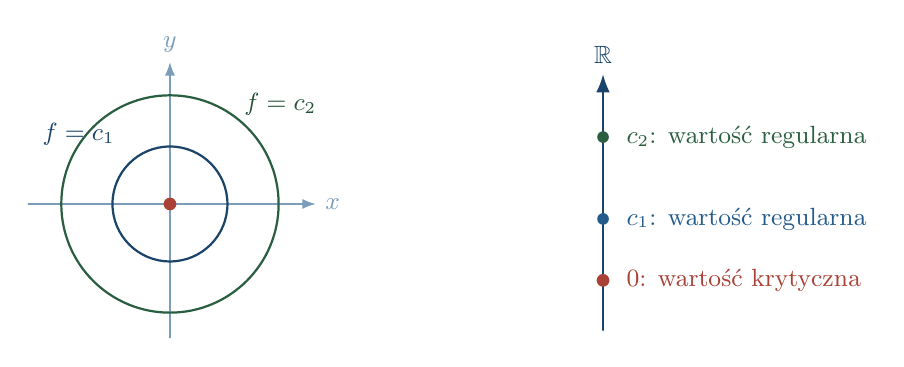
\begin{tikzpicture}[>=Latex,font=\small,line cap=round]
 \begin{scope}[shift={(-2.5,0)}]
  \draw[->,manifoldblue!60] (-1.8,0)--(1.85,0) node[right] {$x$};
  \draw[->,manifoldblue!60] (0,-1.7)--(0,1.8) node[above] {$y$};
  \draw[manifoldblue!75!black,thick] (0,0) circle (.73);
  \draw[manifoldgreen!75!black,thick] (0,0) circle (1.38);
  \fill[manifoldred] (0,0) circle (2.3pt);
  \node[manifoldblue!75!black] at (-1.16,.88) {$f=c_1$};
  \node[manifoldgreen!65!black] at (1.40,1.26) {$f=c_2$};
 \end{scope}
 \begin{scope}[shift={(3,0)}]
  \draw[->,manifoldblue!75!black,thick] (0,-1.6)--(0,1.65)
    node[above] {$\R$};
  \fill[manifoldred] (0,-.97) circle (2.3pt)
    node[right=5pt] {$0$: wartość krytyczna};
  \fill[manifoldblue] (0,-.19) circle (2.1pt)
    node[right=5pt] {$c_1$: wartość regularna};
  \fill[manifoldgreen!75!black] (0,.85) circle (2.1pt)
    node[right=5pt] {$c_2$: wartość regularna};
 \end{scope}
\end{tikzpicture}
\caption{Dla $f(x,y)=x^2+y^2$ punkt krytyczny leży w
dziedzinie, a jego wartość krytyczna na osi wyników.
Poziomice dodatnie są gładkimi okręgami. Schemat
rozróżnia oba pojęcia.}
\label{fig:sard-poziomice}
\end{figure}

\begin{definicja}[Zbiór miary zero na rozmaitości]
\index{zbior miary zero na rozmaitosci@Zbiór miary zero na rozmaitości}
\label{def:sard-zero-miary}
Podzbiór $A\subset\R^n$ ma \emph{miarę zero},
jeśli dla każdego $\varepsilon>0$ można pokryć go
przeliczalnie wieloma kostkami, których suma
$n$-wymiarowych objętości jest mniejsza niż
$\varepsilon$. Zbiór $B\subset N^n$ ma miarę zero,
jeśli dla każdej mapy $(V,\psi)$ rozmaitości $N$
zbiór $\psi(B\cap V)$ ma miarę zero w $\R^n$.
\end{definicja}

Ta definicja nie zależy od mapy. Istotnie, przejście
między dwiema mapami jest gładkim dyfeomorfizmem.
Na każdej zwartej kostce zawartej w dziedzinie przejścia
pochodna jest ograniczona, więc twierdzenie o wartości
średniej daje tam stałą Lipschitza $L$. Jeśli mała kostka
pokrywająca zbiór zerowy ma bok $r$, obraz jej przecięcia
z ustaloną zwartą kostką mieści się w kostce o boku $2L\sqrt n\,r$.
Suma objętości rośnie zatem najwyżej o stały czynnik.
Pokrycia o dowolnie małej sumie objętości pokazują,
że obraz zbioru miary zero znów ma miarę zero. Dziedzinę przejścia można
pokryć przeliczalnie wieloma zwartymi kostkami.
Drugi aksjomat przeliczalności zapewnia także
przeliczalne pokrycie rozmaitości mapami. Z tego
powodu lokalne dowody o mierze zero można
sumować po mapach.

\begin{twierdzenie}[Sarda, wersja gładka]
\label{thm:sard}
Niech $f:M^m\to N^n$ będzie gładkim odwzorowaniem
rozmaitości bez brzegu, $n\geq1$. Zbiór jego
\emph{wartości krytycznych} $f(C(f))$ ma miarę zero
w $N$. W szczególności wartości regularne są gęste
w $N$.
\end{twierdzenie}

\begin{proof}
Wyjaśnimy wszystkie kroki dowodu dla $C^\infty$.
Wybieramy mapy dziedziny tak małe, aby ich obrazy przez
$f$ mieściły się w mapach przeciwdziedziny. Wystarczy więc
rozważyć $f:U\subset\R^m\to\R^n$, z otwartym $U$. Zbiory
$C(f)\cap K$ dla zwartych kostek $K\Subset U$
są zwarte: warunek $\operatorname{rank}\dd f<n$
oznacza znikanie wszystkich minorów rzędu $n$
(jeśli $m<n$, zachodzi automatycznie). Ich obrazy
są więc zwarte, a $f(C(f))$ jest lokalnie
przeliczalną sumą zbiorów zwartych. Wolno
zastosować do nich twierdzenie Fubiniego:
jeżeli każda sekcja takiego mierzalnego zbioru
przez hiperpowierzchnię $\{y_1=t\}$ ma
$(n-1)$-wymiarową miarę zero, to cały zbiór
ma $n$-wymiarową miarę zero.

\emph{Krok 1: źródło mniejszego wymiaru.}
Jeśli $m<n$, na zwartej kostce $Q\Subset U$
odwzorowanie $f$ jest lipschitzowskie.
Podzielmy $Q$ na $k^m$ kostek o boku $a/k$.
Obraz każdej mieści się w kostce o boku
$Ca/k$, zatem suma objętości pokrycia
$f(Q)$ jest co najwyżej
$C'k^m k^{-n}=C'k^{m-n}\to0$.
Stąd cały obraz $f(U)$, a więc tym bardziej
zbiór wartości krytycznych, ma miarę zero.
To daje również początek indukcji po $m$;
dla $m=0$ obraz drugoprzeliczalnej
rozmaitości zerowymiarowej jest przeliczalny.

\emph{Krok 2: punkty krytyczne dodatniego rzędu.}
Załóżmy twierdzenie dla wszystkich odwzorowań
o dziedzinie wymiaru $m-1$ i niech
$x\in C(f)$, ale $\operatorname{rank}\dd f_x>0$.
Po przestawieniu współrzędnych
$\partial f_1/\partial x_1(x)\ne0$.
Twierdzenie o funkcji odwrotnej zastosowane do
\[
 \Phi(x_1,\ldots,x_m)
       =(f_1(x),x_2,\ldots,x_m)
\]
daje dyfeomorfizm pewnego otwartego otoczenia $U_{\mathrm{lok}}$
na jego obraz. W nowych współrzędnych
przepis $f$ ma postać
$g(t,u)=(t,h(t,u))$, gdzie $u\in\R^{m-1}$.
Jeśli $n=1$, ta postać jest submersją,
więc rozważany punkt nie byłby krytyczny.
Przy $n\geq2$ macierz pochodnej ma bloki
\[
 \dd g_{(t,u)}
  =\begin{pmatrix}
       1&0\\ *&\dd_u h(t,u)
    \end{pmatrix},
 \qquad
 \operatorname{rank}\dd g
      =1+\operatorname{rank}\dd h_t(u),
 \quad h_t(u):=h(t,u).
\]
Zatem w sekcji $\{y_1=t\}$ obrazy punktów
krytycznych $g$ pochodzą z wartości krytycznych
$h_t:U_t\to\R^{n-1}$, gdzie
$U_t=\{u:(t,u)\in\Phi(U_{\mathrm{lok}})\}$ jest otwartym
przekrojem nowej dziedziny. Indukcja mówi,
że taka sekcja ma miarę zero. Obraz lokalnego
zbioru punktów krytycznych jest mierzalny
(po wyczerpaniu otwartego otoczenia kostkami
jest sumą obrazów zwartych zbiorów).
Fubini daje miarę zero całego obrazu.
Przeliczalne lokalne otoczenia pokrywają
wszystkie punkty krytyczne dodatniego rzędu.

\emph{Krok 3: punkty o znikających pochodnych.}
Niech $D_k\subset U$ oznacza zbiór punktów,
w których znikają wszystkie pochodne cząstkowe
składowych $f$ rzędów $1,\ldots,k$.
Mamy $D_1\subset C(f)$ oraz
$D_{k+1}\subset D_k$. Jeżeli
$x\in D_k\setminus D_{k+1}$, to pewna pochodna
rzędu $k+1$ jest niezerowa. Wybierzmy
pochodną rzędu $k$ jednej składowej, oznaczoną
przez $w$, której pewna pochodna pierwsza
nie znika w $x$. Ponieważ $w=0$ na $D_k$,
twierdzenie o funkcji uwikłanej mówi, że
$H=\{w=0\}$ jest w otoczeniu $x$ gładką
hiperpowierzchnią zawierającą $D_k$.
Każdy punkt $D_k\cap H$ jest krytyczny dla
$f|_H:H^{m-1}\to\R^n$: już $\dd f=0$
na $D_k$. Na mocy indukcji jego obrazy
tworzą zbiór miary zero. Przeliczalne
pokrycie punktów $D_k\setminus D_{k+1}$
daje tę samą tezę dla całej tej warstwy.

\emph{Krok 4: punkty płaskie do wysokiego rzędu.}
Wybierzmy $k\geq1$ tak duże, że
$n(k+1)>m$. Na zwartej kostce $Q\Subset U$
pochodne rzędu $k+1$ są ograniczone.
Wzór Taylora wokół dowolnego $x\in D_k\cap Q$
ma zerowe składniki rzędów $1,\ldots,k$,
więc dla $y$ w tej samej małej kostce
\[
 |f(y)-f(x)|\leq C|y-x|^{k+1}.
\]
Podzielmy $Q$ na $j^m$ kostek o boku $a/j$.
W każdej, która przecina $D_k$, wybierzmy
takie $x$. Obraz jej punktów należących
do $D_k$ mieści się w kuli promienia
$C'j^{-(k+1)}$. Pokrywając każdą kulę
kostką, dostajemy sumę objętości
co najwyżej $C''j^{m-n(k+1)}\to0$.
Zatem $f(D_k\cap Q)$ ma miarę zero;
liczymy po kostkach wyczerpujących $U$.

Na koniec rozkładamy zbiór krytyczny na
$C(f)\setminus D_1$, warstwy
$D_i\setminus D_{i+1}$ dla $1\leq i<k$
oraz $D_k$. Ich obrazy mają miarę zero
odpowiednio z Kroków~2, 3 i~4.
Przeliczalne pokrycia mapami przenoszą
wynik na $M$ i $N$. Zbiór miary zero
nie zawiera niepustego otwartego podzbioru
$N$, więc wartości regularne są gęste.
\end{proof}

\begin{uwaga}[Zakres twierdzenia]
Sard mówi o \emph{obrazach} punktów krytycznych,
nie o tym, że punktów krytycznych jest mało.
Funkcja stała ma wszystkie punkty krytyczne,
ale tylko jedną wartość krytyczną.
Dla odwzorowań klasy $C^r$ istnieje również
wersja przy założeniu całkowitoliczbowym
$r>\max\{m-n,0\}$; powyższy dowód dotyczy
wersji gładkiej, z której korzystamy dalej.
Jeśli dziedzina ma brzeg, stosujemy wersję bez brzegu
oddzielnie do $f|_{\operatorname{int}M}$ i
$f|_{\partial M}$. Suma ich zbiorów wartości krytycznych
ma miarę zero. Poza nią obie mapy są regularne na
odpowiednich przeciwobrazach; na brzegu surjektywność
$\dd f|_{T\partial M}$ pociąga także surjektywność
$\dd f$ na całym $TM$. Późniejsze twierdzenie o brzegu
wyjaśni, dlaczego potrzebny jest ten silniejszy warunek.
\end{uwaga}

\begin{wniosek}[Typowa poziomica]
\label{cor:sard-poziomica}
Dla prawie każdego $y\in N^n$ zbiór
$f^{-1}(y)$ jest pusty albo gładką
podrozmaitością wymiaru $m-n$, a w każdym
$x\in f^{-1}(y)$
$T_xf^{-1}(y)=\ker\dd f_x$.
\end{wniosek}
\begin{proof}
Poza zbiorem wartości krytycznych z
Twierdzenia~\ref{thm:sard} wartość $y$
jest regularna. Stosujemy
Twierdzenie~\ref{tw:przeciwobraz}; przypadek
pustego przeciwobrazu traktujemy osobno.
\end{proof}

\section{Transwersalność: precyzyjny sens przecięcia}
\label{sec:transwersalnosc}

Wartość regularna to szczególny przypadek
położenia ogólnego. Zamiast punktu $y\in N$
możemy badać trafienie odwzorowania w całą
podrozmaitość $Z\subset N$.

\begin{definicja}[Odwzorowanie transwersalne]
\index{odwzorowanie transwersalne@Odwzorowanie transwersalne}
\label{def:transwersalnosc}
Niech $f:M\to N$ będzie gładkie, a
$Z\subset N$ podrozmaitością zanurzoną w sensie
Rozdziału~\ref{ch:rozmaitosci}. Piszemy
$f\pitchfork Z$, gdy dla każdego
$x\in f^{-1}(Z)$ zachodzi
\begin{equation}\label{eq:transwersalnosc}
 \dd f_x(T_xM)+T_{f(x)}Z=T_{f(x)}N.
\end{equation}
Jeśli $f(M)\cap Z=\varnothing$, warunek jest spełniony
w sposób pusty. Dwie podrozmaitości $A,B\subset N$
przecinają się \emph{transwersalnie},
$A\pitchfork B$, jeśli
$T_xA+T_xB=T_xN$ przy każdym $x\in A\cap B$.
\end{definicja}

Suma w~\eqref{eq:transwersalnosc} jest sumą
\emph{podprzestrzeni}, a nie sumą wektorów
o ustalonych długościach. Jeśli $Z=\{y\}$,
to $T_yZ=0$ i otrzymujemy dokładnie warunek,
że $y$ jest wartością regularną $f$.
Gdy $f$ jest inkluzją $A\hookrightarrow N$,
otrzymujemy definicję transwersalnego
przecięcia $A$ z $Z$.

\begin{figure}[htbp]
\centering
\begin{tikzpicture}[font=\small,line cap=round]
 \begin{scope}[shift={(-2.6,0)}]
  \fill[manifoldblue!5] (-1.75,-1.3) rectangle (1.75,1.3);
  \draw[manifoldblue!85!black,very thick] (-1.45,0)--(1.45,0);
  \draw[manifoldgreen!75!black,very thick] (-1.06,-1.08)--(1.06,1.08);
  \fill[manifoldred] (0,0) circle (2.1pt);
  \node[manifoldblue!75!black] at (1.33,-.23) {$Z$};
  \node[manifoldgreen!65!black] at (.90,1.10) {$A$};
  \node at (0,-1.65) {przecięcie transwersalne};
 \end{scope}
 \begin{scope}[shift={(2.6,0)}]
  \fill[manifoldblue!5] (-1.75,-1.3) rectangle (1.75,1.3);
  \draw[manifoldblue!85!black,very thick] (-1.45,0)--(1.45,0);
  \draw[manifoldgold!80!black,very thick]
     plot[domain=-1.28:1.28,samples=55] (\x,{.63*\x*\x});
  \fill[manifoldred] (0,0) circle (2.1pt);
  \node[manifoldblue!75!black] at (1.33,-.23) {$Z$};
  \node[manifoldgold!75!black] at (1.25,1.12) {$A$};
  \node at (0,-1.65) {styczność: brak transwersalności};
 \end{scope}
\end{tikzpicture}
\caption{Po lewej dwie proste w płaszczyźnie mają
różne kierunki styczne, które razem rozpinają
$T_p\R^2$. Po prawej parabola dotyka osi:
obie przestrzenie styczne są tą samą prostą.}
\label{fig:transwersalne-przeciecia}
\end{figure}

\begin{twierdzenie}[Przeciwobraz podrozmaitości]
\label{thm:transwersalny-przeciwobraz}
Niech $Z\subset N^n$ będzie podrozmaitością
zanurzoną kowymiaru $c$, a $f:M^m\to N$
niech spełnia $f\pitchfork Z$. Wtedy
$f^{-1}(Z)$ jest pusty albo jest
podrozmaitością zanurzoną wymiaru $m-c$.
W punkcie $x\in f^{-1}(Z)$ zachodzi
\begin{equation}\label{eq:transwersalny-styczna}
 T_xf^{-1}(Z)
  =(\dd f_x)^{-1}\bigl(T_{f(x)}Z\bigr).
\end{equation}
Jeśli $m<c$, przeciwobraz jest pusty.
\end{twierdzenie}
\begin{proof}
Wokół $z=f(x)$ wybierzmy mapę
$\psi:V\to\R^{n-c}\times\R^c$, w której
$\psi(Z\cap V)=\psi(V)\cap(\R^{n-c}\times\{0\})$.
Niech $h=\operatorname{pr}_{\R^c}\circ\psi$.
Wtedy lokalnie $Z=h^{-1}(0)$ oraz
$\ker\dd h_z=T_zZ$.
Reguła łańcucha pokazuje, że
$\dd(h\circ f)_x=\dd h_z\circ\dd f_x$.
Ta różniczka jest surjekcją na $\R^c$
dokładnie wtedy, gdy
$\dd f_x(T_xM)+\ker\dd h_z=T_zN$;
jest to~\eqref{eq:transwersalnosc}.
Zatem $0$ jest lokalnie wartością regularną
$h\circ f$. Twierdzenie~\ref{tw:przeciwobraz}
daje podrozmaitość kowymiaru $c$ i
\[
 \ker\dd(h\circ f)_x
  =\{v:\dd f_xv\in\ker\dd h_z\},
\]
co jest~\eqref{eq:transwersalny-styczna}.
Jeśli $m<c$, surjekcja $\R^m\to\R^c$
nie istnieje. Nie może więc istnieć punkt
przeciwobrazu przy założonej transwersalności.
\end{proof}

\begin{przyklad}[Prosta i parabola]
W $N=\R^2$ niech $Z=\{(x,0)\}$.
Dla $f(t)=(t,t)$ mamy
$f^{-1}(Z)=\{0\}$ oraz
$\dd f_0(\R)=\operatorname{span}(1,1)$,
który wraz z $T_{(0,0)}Z=\operatorname{span}(1,0)$
rozpina $\R^2$. Dla $g(t)=(t,t^2)$
przeciwobraz także jest pojedynczym punktem,
ale $\dd g_0(\R)=T_{(0,0)}Z$:
sam fakt, że punktów przecięcia jest skończenie
wiele, \emph{nie} oznacza transwersalności.
Na Rysunku~\ref{fig:transwersalne-przeciecia}
przedstawiono oba przypadki.
\end{przyklad}

\begin{twierdzenie}[Przecięcie i iloczyn włóknisty]
\label{thm:transwersalne-przeciecie}
Jeżeli podrozmaitości $A^a,B^b\subset N^n$
spełniają $A\pitchfork B$, to $A\cap B$
jest pusty albo jest podrozmaitością wymiaru $a+b-n$ oraz
\[
 T_x(A\cap B)=T_xA\cap T_xB.
\]
Ogólniej, dla gładkich $f:M^m\to N^n$ i
$g:P^p\to N^n$ załóżmy, że przy każdym
$f(x)=g(y)=z$ mamy
\begin{equation}\label{eq:transwersalne-dwa-odwz}
 \dd f_x(T_xM)+\dd g_y(T_yP)=T_zN.
\end{equation}
Wówczas
$M\times_N P=\{(x,y):f(x)=g(y)\}$
jest pusty albo jest podrozmaitością $M\times P$ wymiaru
$m+p-n$, a jej przestrzeń styczna składa się z
par $(u,v)$ spełniających $\dd f_xu=\dd g_yv$.
\end{twierdzenie}
\begin{proof}
Niech $\Delta_N=\{(z,z):z\in N\}$ będzie diagonalą
w $N\times N$. Jej przestrzeń styczna w $(z,z)$
to $\{(w,w):w\in T_zN\}$. Obliczamy
\[
 T_{(z,z)}(N\times N)/T_{(z,z)}\Delta_N
       \cong T_zN,\qquad [(u,v)]\longmapsto u-v.
\]
Odwzorowanie $(f,g):M\times P\to N\times N$
jest transwersalne do diagonali dokładnie wtedy,
gdy $(u,v)\mapsto\dd f_xu-\dd g_yv$ jest surjekcją,
czyli gdy zachodzi~\eqref{eq:transwersalne-dwa-odwz}.
Twierdzenie~\ref{thm:transwersalny-przeciwobraz}
daje podrozmaitość kowymiaru $n$.
Jej przestrzeń styczna jest jądrem powyższej
różnicy, skąd oba wzory. Dla inkluzji
$A\hookrightarrow N$ i $B\hookrightarrow N$
iloczyn włóknisty utożsamiamy z $A\cap B$
przez $(z,z)\mapsto z$. Warunek staje się
$T_zA+T_zB=T_zN$, a jądro jest przecięciem
obu przestrzeni stycznych.
\end{proof}

\begin{uwaga}[Oczekiwany wymiar]
Liczba $a+b-n$ to \emph{oczekiwany wymiar}
przecięcia. Ujemny wynik wymusza pustkę przy
transwersalności. Wynik zero oznacza izolowane
punkty przecięcia. Jeśli $A$ jest zwarta, a $B$ domknięta
(w szczególności gdy obie są zwarte), przecięcie jest
zwarte i dyskretne, więc skończone. Sama dyskretność
bez zwartości nie wyklucza nieskończenie wielu punktów.
To właśnie przypadek, w którym później można
liczyć przecięcia ze znakami, używając orientacji
z Sekcji~\ref{sec:formy-orientacja}.
\end{uwaga}

\section{Brzeg i kontrola miejsca przecięcia}
\label{sec:transwersalnosc-brzeg}

W konstrukcjach topologicznych pojawiają się
przestrzenie z brzegiem. Sam warunek
$f\pitchfork Z$ we wnętrzu nie gwarantuje
poprawnego zachowania przeciwobrazu na brzegu.

\begin{twierdzenie}[Przeciwobraz transwersalny z brzegiem]
\label{thm:transwersalnosc-brzeg}
Niech $M^m$ będzie rozmaitością z brzegiem,
$N$ bez brzegu, $Z\subset N$ podrozmaitością
kowymiaru $c$. Jeżeli zarówno $f:M\to N$,
jak i $f|_{\partial M}:\partial M\to N$
są transwersalne do $Z$, to
$W=f^{-1}(Z)$ jest pusty albo jest rozmaitością z brzegiem
wymiaru $m-c$ i
\[
 \partial W=W\cap\partial M.
\]
\end{twierdzenie}
\begin{proof}
We wnętrzu $M$ stosujemy
Twierdzenie~\ref{thm:transwersalny-przeciwobraz}.
Przy $x\in\partial M\cap W$ wybierzmy współrzędne
półprzestrzeni $(r,u_2,\ldots,u_m)$,
$r\geq0$, oraz lokalną funkcję definiującą
$Z$, $h:N\to\R^c$ jak w poprzednim dowodzie.
Połóżmy $H=h\circ f$. Transwersalność
$f|_{\partial M}$ oznacza, że
$\dd H_x:T_x\partial M\to\R^c$ jest surjekcją.
Możemy więc wybrać $c$ kierunków
\emph{stycznych do brzegu}, na których
współrzędne $H$ tworzą niezależny układ.
Po przestawieniu zmiennych $u$ odpowiedni minor $c\times c$
jest odwracalny. Gładkość na półprzestrzeni pozwala
przedłużyć $H$ lokalnie przez $r=0$. Twierdzenie o funkcji
odwrotnej dla mapy $(r,u)\mapsto(r,H(r,u),v)$ stosujemy
w tym otwartym otoczeniu, a potem ograniczamy do $r\geq0$.
Jej różniczka jest odwracalna właśnie dzięki wybranemu
minorowi i zachowaniu pozostałych współrzędnych.
Ponieważ $r$ pozostało współrzędną brzegową,
zbiór $H=0$ ma w tych współrzędnych postać
$\{(r,0,v):r\geq0\}$. Jego brzeg jest dokładnie
$\{r=0,H=0\}=W\cap\partial M$.
Pozostałe $m-1-c$ współrzędne $v$ wraz z $r$
dają wymiar $m-c$. Przy $m<c$ cały przeciwobraz jest
pusty; przy $m=c$ nie może spotykać brzegu, ponieważ
surjekcja z jego $(m-1)$-wymiarowej przestrzeni stycznej
na $\R^c$ nie istnieje.
\end{proof}

\begin{przyklad}[Dlaczego warunek na brzegu jest potrzebny]
Weźmy górną półpłaszczyznę
$M=\{(x,y)\in\R^2:y\geq0\}$,
$N=\R$ i $Z=\{0\}$. Funkcja $f(x,y)=y$
jest submersją w każdym punkcie $M$,
lecz jej ograniczenie do brzegu jest stale
równe zero. Mamy $f^{-1}(0)=\partial M$,
czyli prostą \emph{bez} brzegu; równość
$\partial f^{-1}(Z)=f^{-1}(Z)\cap\partial M$
byłaby tutaj fałszywa. W praktyce należy
sprawdzać oba warunki osobno.
\end{przyklad}

\section{Transwersalność z parametrem}
\label{sec:transwersalnosc-param}

Nie należy rozumieć „ogólnego położenia” jako
założenia o losowości rysunku. Chodzi o precyzyjne
twierdzenie: w gładkiej rodzinie dopuszczalnych
przesunięć złe parametry tworzą zbiór miary zero.

\begin{twierdzenie}[Transwersalność parametryczna]
\label{thm:transwersalnosc-param}
Niech $M,A,N$ będą gładkimi rozmaitościami bez brzegu,
$Z\subset N$ podrozmaitością zanurzoną, a
$F:M\times A\to N$ gładkim odwzorowaniem.
Jeżeli $F\pitchfork Z$, to dla prawie każdego
$a\in A$ odwzorowanie $F_a(x)=F(x,a)$ spełnia
$F_a\pitchfork Z$. W szczególności takie
parametry są gęste w $A$.
\end{twierdzenie}
\begin{proof}
Ponieważ $F\pitchfork Z$,
$W=F^{-1}(Z)$ jest podrozmaitością
$M\times A$ na mocy
Twierdzenia~\ref{thm:transwersalny-przeciwobraz}.
Rozważmy rzutowanie $\pi:W\to A$.
W punkcie $(x,a)\in W$, $z=F(x,a)$,
\[
 T_{(x,a)}W
 =\{(u,b):\dd_xF_{(x,a)}u
              +\dd_aF_{(x,a)}b\in T_zZ\}.
\]
Zatem $\dd\pi_{(x,a)}$ jest surjekcją
dokładnie wtedy, gdy dla każdego $b\in T_aA$
można dobrać $u\in T_xM$ tak, aby
$\dd_aF(b)+\dd_xF(u)\in T_zZ$.
Inaczej mówiąc,
\[
 \dd_aF(T_aA)\subset
                 \dd_xF(T_xM)+T_zZ.
\]
Łącznie z założeniem
$\dd_xF(T_xM)+\dd_aF(T_aA)+T_zZ=T_zN$
jest to równoważne
$\dd_xF(T_xM)+T_zZ=T_zN$, czyli
transwersalności $F_a$ w punkcie $x$.
Wartość $a$ jest regularna dla $\pi$
wtedy i tylko wtedy, gdy $F_a$ jest
transwersalne do $Z$ we wszystkich punktach
przeciwobrazu. Sard zastosowany do
$\pi:W\to A$ kończy dowód, jeśli $\dim A\geq1$.
Dla $\dim A=0$ przestrzeń parametrów jest dyskretna,
a $T_aA=0$. Wtedy $\dd F=\dd_xF$ na każdej składowej
$M\times\{a\}$ i założenie daje tezę dla każdego $a$,
bez odwoływania się do Sarda.
\end{proof}

\begin{przyklad}[Rozszczepienie stycznego przecięcia]
\label{prz:transwersalne-parabola}
Niech $M=N=\R$, $Z=\{0\}$ oraz
$F(t,a)=t^2-a$. Pochodna w kierunku parametru
wynosi $\partial_aF=-1$, więc cała rodzina
$F:\R^2\to\R$ jest submersją.
Dla $a>0$ mapa $F_a$ ma dwa regularne zera
$t=\pm\sqrt a$, bo $F_a'(t)=2t\ne0$.
Dla $a<0$ nie ma zer, a $a=0$ daje
styczne, nieregularne zero $t=0$.
Jedyny zły parametr to $0$.
\end{przyklad}

\begin{figure}[htbp]
\centering
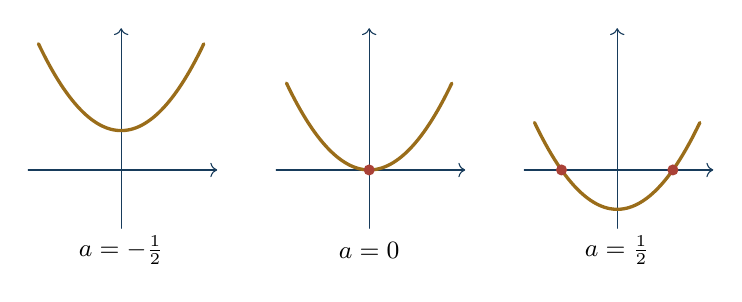
\begin{tikzpicture}[font=\small,line cap=round]
 \foreach \panel/\aval/\lab in {-3.15/-.5/$a=-\frac12$,0/0/$a=0$,3.15/.5/$a=\frac12$}{
  \begin{scope}[shift={(\panel,0)}]
   \draw[->,manifoldblue!65!black] (-1.18,0)--(1.22,0);
   \draw[->,manifoldblue!65!black] (0,-.74)--(0,1.80);
   \draw[manifoldgold!75!black,very thick]
    plot[domain=-1.05:1.05,samples=60,variable=\t]
       (\t,{(\t)^2-(\aval)});
   \node at (0,-1.02) {\lab};
  \end{scope}
 }
 \fill[manifoldred] (0,0) circle (2pt);
 \fill[manifoldred] ({3.15-sqrt(.5)},0) circle (2pt);
 \fill[manifoldred] ({3.15+sqrt(.5)},0) circle (2pt);
\end{tikzpicture}
\caption{Poziom zero rodziny $F_a(t)=t^2-a$.
Zmiana parametru rozbija styczność w dwa
przecięcia transwersalne albo usuwa przecięcie;
sam parametr $a=0$ jest wyjątkowy.}
\label{fig:transwersalnosc-perturbacja}
\end{figure}

Twierdzenie parametryczne nie mówi jeszcze, że
\emph{każde} konkretne odwzorowanie ma dostatecznie
bogatą rodzinę perturbacji. Przy zwartej dziedzinie
możemy taką rodzinę zbudować bez odwoływania się
do twierdzenia Whitneya o zanurzeniach.

Wyjaśnijmy używaną tu topologię przybliżania. Wybierzmy
skończenie wiele map $x_i$ w $M$ i $y_i$ w $N$ oraz
zwartych zbiorów $K_i$ w dziedzinach $x_i$ tak, by ich
wnętrza pokrywały $M$, a $f(K_i)$ leżały w dziedzinach $y_i$.
Zapewniają to ciągłość $f$ i zwartość $M$.
Dla odwzorowań $g$ bliskich $f$ wymagamy
$g(K_i)$ w tych samych mapach i kontrolujemy liczby
\[
 \max_i\max_{|\alpha|\leq r}\sup_{u\in x_i(K_i)}
 \left|\partial^\alpha(y_i\circ g\circ x_i^{-1})(u)
       -\partial^\alpha(y_i\circ f\circ x_i^{-1})(u)\right|.
\]
Małość tych liczb określa topologię $C^r$. Reguła łańcucha
i zwartość pokazują, że zmiana skończonego układu map
daje tę samą topologię. Topologia $C^\infty$ jest generowana
przez te warunki dla wszystkich skończonych $r$:
zbieżność oznacza zbieżność w każdym $C^r$, a podstawowe
otoczenie zadaje tylko skończenie wiele takich ograniczeń.
Nie wymagamy jednego oszacowania jednocześnie dla
pochodnych wszystkich rzędów.

\begin{twierdzenie}[Przybliżanie odwzorowań transwersalnymi]
\label{thm:gestosc-transwersalnych}
Niech $M$ będzie zwartą rozmaitością bez brzegu,
$N$ rozmaitością, a $Z\subset N$ podrozmaitością
zanurzoną. Każde gładkie $f:M\to N$ można
dowolnie blisko przybliżyć w topologii $C^\infty$
gładkim $g:M\to N$ transwersalnym do $Z$.
Można przy tym wybrać gładką homotopię
od $f$ do $g$.
Jeśli dodatkowo $Z$ jest domknięta w $N$,
transwersalność jest otwarta w topologii $C^1$
na gładkich odwzorowaniach z $M$ do $N$.
\end{twierdzenie}
\begin{proof}
\emph{Budowa skończonej liczby kierunków perturbacji.}
Wybierzmy na $N$ dowolną metrykę riemannowską.
Przeciągnięta wiązka $f^*TN$ ma nad małymi
otoczeniami $U_i\subset M$ gładkie ramy.
Ponieważ $M$ jest zwarta, możemy wybrać skończenie
wiele mniejszych $V_i\Subset U_i$, które pokrywają
$M$. Dla każdego $i$ wybierzmy funkcję odcinającą
$\rho_i$, równą $1$ na $V_i$ i o nośniku w $U_i$.
Pomnóżmy każdy wektor lokalnej ramy $f^*TN|_{U_i}$
przez $\rho_i$ i przedłużmy przez zero. Otrzymujemy
skończenie wiele globalnych przekrojów
$s_1,\ldots,s_k$ wiązki $f^*TN$ takich, że
ich wartości rozpinają $T_{f(x)}N$ w każdym $x$.

Niech $a=(a_1,\ldots,a_k)$ przebiega małą kulę
w $\R^k$. Definiujemy
\[
 F(x,a)=\exp^N_{f(x)}
              \left(\sum_{j=1}^k a_js_j(x)\right).
\]
Metryka nie musi być zupełna: wykładnicze
odwzorowanie jest określone przy wektorze zero,
a zwartość $M$ pozwala wziąć jedną wystarczająco
małą kulę parametrów dla wszystkich $x$.
W punkcie $a=0$ pochodna $F$ względem parametrów
przyjmuje na standardowym kierunku $j$ wartość
$s_j(x)$, ponieważ $\dd(\exp^N_{f(x)})_0=\id$.
Jest więc surjektywna na $T_{f(x)}N$.
Surjektywność jest warunkiem otwartym;
przez zwartość $M$ pozostaje prawdziwa na
$M\times A$ po zmniejszeniu kuli $A$.
Cała mapa $F$ jest zatem submersją,
w szczególności $F\pitchfork Z$.
Twierdzenie~\ref{thm:transwersalnosc-param}
dostarcza parametrów $a$ transwersalnych do
$Z$ dowolnie blisko zera. Dla
$g=F_a$ mamy $F_a\to F_0=f$ w $C^\infty$:
w ustalonych mapach każda pochodna po $x$ zależy
ciągle od $(x,a)$, a na skończonym pokryciu zwartych
$K_i$ zbieżność przy $a\to0$ jest jednostajna dla każdego
skończonego rzędu. Ścieżka $t\mapsto F_{ta}$ daje
gładką homotopię, ponieważ kula $A$ jest wypukła.

\emph{Otwartość przy domkniętym $Z$.}
Załóżmy, że $f\pitchfork Z$, lecz pewne
$f_j\to f$ w $C^1$ nie są transwersalne.
Wybierzmy punkty $x_j$ naruszenia warunku.
Po przejściu do podciągu $x_j\to x$ dzięki
zwartości $M$. Ponieważ $Z$ jest domknięta,
$f(x)=\lim f_j(x_j)$ należy do $Z$.
W lokalnej mapie spłaszczającej $Z$
transwersalność oznacza, że ustalony
minor macierzy pochodnej normalnych
współrzędnych jest niezerowy. Dla $f$
jest taki minor w $x$; ciągłość i zbieżność
$C^1$ dają ten sam niezerowy minor dla
$f_j$ w $x_j$ przy dużym $j$.
Otrzymujemy sprzeczność.
\end{proof}

\begin{wniosek}[Perturbacja względna]
\label{cor:transwersalnosc-wzgledna}
Załóżmy dodatkowo w poprzednim twierdzeniu,
że $Z$ jest domknięta i $f\pitchfork Z$
na otoczeniu domkniętego $C\subset M$.
Wówczas $g$ można wybrać równe $f$
na pewnym otoczeniu $C$.
\end{wniosek}
\begin{proof}
Wybierzmy otoczenia
$C\subset U_0\Subset U_1\Subset U$,
gdzie $f\pitchfork Z$ na $U$.
Powtórzmy konstrukcję przekrojów z poprzedniego
dowodu tylko nad zwartym zbiorem
$M\setminus U_1$, dobierając ich nośniki
w $M\setminus\overline U_0$.
Otrzymana rodzina $F_a$ jest identyczna z
$f$ na $U_0$, a jej pochodna parametryczna
rozpina $TN$ na $M\setminus U_1$.
Na zwartym $\overline U_1\subset U$ dostatecznie małe
perturbacje zachowują transwersalność $f$. Stosujemy
tu dowód otwartości na zwartym podzbiorze, nie twierdzenie
o rozmaitości $\overline U_1$: hipotetyczne punkty
naruszenia miałyby podciąg z granicą w $\overline U_1$,
a ten sam argument z niezerowym minorem dawałby sprzeczność.
Stąd cała rodzina $F:M\times A\to N$
jest transwersalna do $Z$.
Wybieramy parametr z
Twierdzenia~\ref{thm:transwersalnosc-param}
dowolnie blisko zera. Na $U_0$ wynikowe
$g=F_a$ jest dokładnie $f$. Cała homotopia $F_{ta}$
również pozostaje tam równa $f$.
\end{proof}

Jeśli $M$ ma brzeg, a rodzina $F$ i jej
ograniczenie $F|_{\partial M\times A}$
są transwersalne do $Z$, można zastosować
Sarda do dwóch map bez brzegu:
$\pi|_{\operatorname{int}W}$ oraz $\pi|_{\partial W}$,
gdzie $W=F^{-1}(Z)$ i $\partial W=W\cap(\partial M\times A)$.
Pierwsza kontroluje transwersalność $F_a$ we wnętrzu,
druga transwersalność jego ograniczenia do brzegu.
Ta ostatnia pociąga też transwersalność $F_a$ na całej
przestrzeni stycznej $T_xM$ w punkcie brzegowym.
Suma dwóch zbiorów parametrów wyjątkowych
nadal ma miarę zero. Dla pozostałych
parametrów otrzymujemy oba warunki
Twierdzenia~\ref{thm:transwersalnosc-brzeg}.

\section{Zera przekrojów i punkty krytyczne funkcji}
\label{sec:transwersalnosc-przekroje}

Nie każdy problem ma postać przecięcia dwóch
podzbiorów jednej przestrzeni. Często szukamy
zer pola wektorowego, $1$-formy albo innego
przekroju wiązki. Wtedy transwersalność działa
względem \emph{przekroju zerowego}.

\begin{twierdzenie}[Regularne zera przekroju]
\label{thm:zera-przekroju}
Niech $E\to M^m$ będzie wiązką wektorową
rzędu $r$, a $s:M\to E$ gładkim przekrojem.
W lokalnej trywializacji $s(x)=(x,\sigma(x))$.
W punkcie $s(x)=0$ pochodna
$\D_xs:=\dd\sigma_x:T_xM\to E_x$
nie zależy od wyboru trywializacji
po naturalnym utożsamieniu włókien.
Jeżeli $\D_xs$ jest surjektywna przy
każdym zerze, to zbiór zer $s^{-1}(0_E)$
jest pusty albo jest podrozmaitością kowymiaru $r$, a
$T_xs^{-1}(0_E)=\ker\D_xs$.
\end{twierdzenie}
\begin{proof}
W trywializacji przekrój zerowy ma postać
$\{(x,0)\}$, a kierunki normalne do niego
odpowiadają współrzędnym włókna.
Różniczka $s(x)=(x,\sigma(x))$ ma postać
$v\mapsto(v,\dd\sigma_xv)$. Warunek
$s\pitchfork 0_E$ jest więc dokładnie
surjektywnością $\dd\sigma_x$.
Twierdzenie~\ref{thm:transwersalny-przeciwobraz}
daje wymiar i przestrzeń styczną.
Przy zmianie trywializacji
$\widetilde\sigma(y)=A(y)\sigma(y)$,
gdzie $A(y)$ jest odwracalną macierzą.
W punkcie z $\sigma(x)=0$ reguła iloczynu
daje $\dd\widetilde\sigma_x=A(x)\dd\sigma_x$:
wyraz $(\dd A_x)\sigma(x)$ znika.
Surjektywność i jądro nie zależą więc
od trywializacji. W sposób wewnętrzny w zerze $s(x)$
mamy kanoniczny rozkład
$T_{0_x}E\cong T_xM\oplus E_x$: pierwsza część jest
styczna do przekroju zerowego, a druga jest pionowa.
Pionowa składowa $\dd s_x$ to właśnie $\D_xs$.
Dla $r>m$ surjekcja jest niemożliwa, więc przekrój
transwersalny nie ma zer.
\end{proof}

\begin{przyklad}[Zera pola na płaszczyźnie]
Pole $X(x,y)=x\,\partial_x+y\,\partial_y$ ma
jedno zero, a jego pochodna pionowa w zerze
jest macierzą jednostkową: zero jest
transwersalne. Pole
$Y(x,y)=x^2\partial_x+y\,\partial_y$
też ma jedno zero, lecz macierz
$\D_0Y=\operatorname{diag}(0,1)$
nie jest surjektywna. Sama izolacja zera
nie wystarcza do transwersalności.
\end{przyklad}

Dla funkcji $f:M\to\R$ przekrojem, który
nas interesuje, jest $df:M\to T^*M$.
To pozwala wyjaśnić, skąd w przyszłej
teorii Morse'a pojawia się hesjan.

\begin{definicja}[Hesjan i niezdegenerowany punkt krytyczny]
\index{hesjan i niezdegenerowany punkt krytyczny@Hesjan i niezdegenerowany punkt krytyczny}
\label{def:morse-pochodna}
Jeśli $\dd f_p=0$, to w dowolnej mapie
$(x^1,\ldots,x^m)$ wokół $p$ definiujemy
\[
 \operatorname{Hess}_p f(v,w)
 =\sum_{i,j}
    \frac{\partial^2 f}{\partial x^i\partial x^j}(p)
                   v^iw^j.
\]
Punkt $p$ nazywamy \emph{niezdegenerowanym},
gdy ta forma dwuliniowa ma nieosobliwą macierz.
Funkcja, której wszystkie punkty krytyczne
są niezdegenerowane, nazywa się
\emph{funkcją Morse'a}.
\end{definicja}

Hesjan w punkcie krytycznym jest niezależny
od mapy. Druga pochodna złożenia
$f\circ\varphi^{-1}$ z przejściem współrzędnych
ma wyraz z drugą pochodną $f$ przeniesiony
przez jakobian oraz wyraz z pierwszą pochodną
$f$ pomnożoną przez drugie pochodne przejścia.
Ten ostatni wyraz znika właśnie dlatego,
że $\dd f_p=0$. Dokładniej, jeśli $x=x(y)$ jest zmianą map,
to w punkcie krytycznym
\[
 \frac{\partial^2 f}{\partial y^a\partial y^b}(p)
 =\sum_{i,j}\frac{\partial x^i}{\partial y^a}(p)
             \frac{\partial x^j}{\partial y^b}(p)
             \frac{\partial^2 f}{\partial x^i\partial x^j}(p).
\]
Jest to prawo transformacji formy dwuliniowej,
$H_y=J^{\mathsf T}H_xJ$, więc niezdegenerowanie jest
niezależne od mapy. Po wyborze dowolnej koneksji
Leviego-Civity wcześniejszy hesjan ma współrzędne
$(\nabla df)_{ij}=\partial_i\partial_jf-\Gamma^k_{ij}\partial_kf$;
w punkcie krytycznym daje tę samą formę. Nie wymaga
ona zatem wyboru metryki w tym punkcie.
W mapie wiązki kostycznej
przekrój $df$ ma współrzędne
$(x,(\partial_1f,\ldots,\partial_m f))$.
Jego pochodna pionowa w punkcie krytycznym
jest więc macierzą
$(\partial_i\partial_j f)(p)$. Dostajemy
równoważność
\begin{equation}\label{eq:morse-transwersalnosc}
 df\pitchfork 0_{T^*M}
 \quad\Longleftrightarrow\quad
 \text{każdy punkt krytyczny $f$ jest
 niezdegenerowany.}
\end{equation}

\begin{twierdzenie}[Istnienie i typowość funkcji Morse'a]
\label{thm:gestosc-morse}
Na każdej zwartej rozmaitości gładkiej
bez brzegu funkcje Morse'a są gęste wśród
funkcji gładkich w topologii $C^\infty$
i tworzą zbiór otwarty w topologii $C^2$.
Każda taka funkcja ma skończenie wiele
punktów krytycznych. Można dodatkowo
osiągnąć, by ich wartości były parami różne.
\end{twierdzenie}
\begin{proof}
\emph{Gęstość.}
Weźmy skończone mapy $(U_i,x_i^1,\ldots,x_i^m)$
i funkcje odcinające $\rho_i$ tak, aby mniejsze
obszary, na których $\rho_i=1$, pokrywały $M$,
a $\operatorname{supp}\rho_i\Subset U_i$.
Funkcje $\rho_i x_i^j$, przedłużone przez
zero poza $U_i$, są globalnie gładkie.
Niech
\[
 f_a=f+\sum_{i,j}a_{ij}\rho_i x_i^j.
\]
W dowolnym $x$ leżącym w mniejszym obszarze
mapy $i$ mamy
$\dd(\rho_i x_i^j)_x=\dd x_i^j$.
Kowektory te tworzą bazę $T_x^*M$.
Zatem parametryczna rodzina przekrojów
$(x,a)\mapsto df_a(x)$ ma surjektywną
pochodną pionową w kierunkach $a$:
jest transwersalna do przekroju zerowego
$0_{T^*M}$. Twierdzenie
~\ref{thm:transwersalnosc-param}
zastosowane do tej rodziny mówi, że
dla prawie każdego małego $a$ przekrój
$df_a$ jest transwersalny do zera.
Równoważność~\eqref{eq:morse-transwersalnosc}
czyni $f_a$ funkcją Morse'a. Ponieważ
$a\to0$ można wybrać dowolnie,
$f_a\to f$ w $C^\infty$.

\emph{Otwartość i skończoność.}
Jeśli $f$ jest Morse'a, przekrój $df$
jest transwersalny do domkniętego
przekroju zerowego. Dowód otwartości
z Twierdzenia~\ref{thm:gestosc-transwersalnych}
stosuje się także do przekrojów;
gdy $g$ jest bliskie $f$ w $C^2$,
$dg$ jest bliskie $df$ w $C^1$.
To daje otwartość. Zbiór krytyczny
jest zerowymiarową podrozmaitością
na mocy Twierdzenia~\ref{thm:zera-przekroju},
więc jego punkty są izolowane.
Jest także zamknięty w zwartym $M$;
zatem jest skończony.

\emph{Różne wartości.}
Niech krytyczne punkty funkcji Morse'a
będą $p_1,\ldots,p_\ell$. Wybierzmy
rozłączne małe otoczenia i funkcje
odcinające $\beta_i$ równe $1$ w jeszcze
mniejszych otoczeniach $p_i$.
Zastąpmy $f$ przez
$f+\sum_i c_i\beta_i$.
Przy dostatecznie małych $c_i$ w obszarach,
gdzie zmieniają się $\beta_i$, nie pojawiają
się nowe punkty krytyczne: na zwartym
zbiorze tych obszarów $|\dd f|$ ma dodatnie
minimum, a $|\sum_i c_i\dd\beta_i|$ może
być od niego mniejsze. W pobliżu $p_i$
nowa funkcja różni się od $f$ o stałą
$c_i$, więc zachowuje punkty i hesjany.
Nowe wartości to $f(p_i)+c_i$; wybieramy
małe $c_i$ poza skończoną sumą hiperpłaszczyzn
$f(p_i)+c_i=f(p_j)+c_j$.
\end{proof}

\begin{przyklad}[Mała perturbacja funkcji]
Na $\R^2$ funkcja $f(x,y)=x^2$ ma całą prostą
$x=0$ punktów krytycznych; hesjan
$\operatorname{diag}(2,0)$ jest osobliwy.
Po dodaniu $\varepsilon y^2$ (perturbacji małej wraz
z pochodnymi na każdym ustalonym zbiorze zwartym) dla
$\varepsilon\ne0$ pozostaje tylko punkt
$(0,0)$, a hesjan
$\operatorname{diag}(2,2\varepsilon)$
jest odwracalny. Gdy $\varepsilon>0$
otrzymujemy minimum, a gdy
$\varepsilon<0$ punkt siodłowy.
To lokalny obraz perturbacji; twierdzenie
poprzednie zapewnia analogiczne
rozwiązanie globalne na zwartej rozmaitości.
\end{przyklad}

\section{Dlaczego transwersalność pojawi się u Smale'a?}
\label{sec:transwersalnosc-smale}

Niech $(M^n,g)$ będzie rozmaitością riemannowską,
a $f:M\to\R$ funkcją Morse'a,
a $X=-\nabla_g f$ jej polem spadku. W punkcie
krytycznym $p$ \emph{indeks Morse'a}
$\lambda(p)$ to liczba ujemnych wartości
własnych formy $\operatorname{Hess}_p f$
po podniesieniu jednego indeksu metryką $g$,
liczonych z krotnościami. Prawo bezwładności Sylvestera
pokazuje, że ta liczba zależy od formy hesjanu,
a nie od pomocniczej metryki użytej do wyznaczenia
wartości własnych. W dalszej teorii
przepływu gradientowego skonstruujemy
rozmaitość niestabilną $W^u(p)$, złożoną
z punktów dążących do $p$ przy czasie
$t\to-\infty$, oraz stabilną $W^s(q)$,
złożoną z punktów dążących do $q$
przy $t\to+\infty$. W tych definicjach wymagamy
istnienia trajektorii przez całą odpowiednią półprostą
czasu. Na zwartej rozmaitości jest to automatyczne;
gdy pole nie jest zupełne, nie wolno tego pomijać.
Twierdzenie o
rozmaitościach stabilnych daje
\[
 \dim W^u(p)=\lambda(p),\qquad
 \dim W^s(q)=n-\lambda(q).
\]
Nie dowodzimy tutaj tego twierdzenia o równaniach
różniczkowych; poniżej wyprowadzamy już teraz
\emph{konsekwencję transwersalności} tych obiektów.
Globalnie traktujemy je jako rozmaitości z immersjami
do $M$; lokalnie każda wybrana gałąź jest podrozmaitością
z mapą plasterkową. Wniosek poniżej dotyczy takiego
lokalnego przecięcia, co nie wymaga z góry twierdzenia
o globalnym zanurzeniu obu zbiorów.

\begin{przyklad}[Siodło i dwa kierunki przepływu]
\label{prz:siodlo-transwersalne}
W $\R^2$ dla metryki euklidesowej i
$f(x,y)=x^2-y^2$ pole spadku wynosi
$X=(-2x,2y)$. Rozwiązanie startujące z
$(x_0,y_0)$ jest jawne:
\[
 x(t)=x_0e^{-2t},\qquad y(t)=y_0e^{2t}.
\]
Do $(0,0)$ przy $t\to+\infty$ dążą dokładnie
punkty z $y_0=0$, więc
$W^s(0)=\{y=0\}$. Przy $t\to-\infty$
dążą punkty z $x_0=0$, więc
$W^u(0)=\{x=0\}$. Ich styczne w siodle
rozpinają $\R^2$, jak przewiduje
nieosobliwy hesjan $\operatorname{diag}(2,-2)$.
\end{przyklad}

\begin{figure}[htbp]
\centering
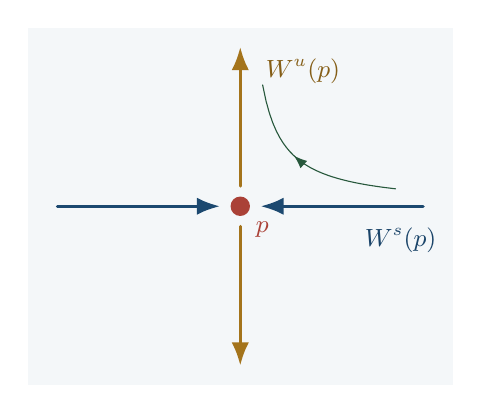
\begin{tikzpicture}[>=Latex,font=\small,line cap=round,scale=1.35]
 \fill[manifoldblue!5] (-2,-1.68) rectangle (2,1.68);
 \draw[->,manifoldblue!80!black,very thick] (-1.72,0)--(-.19,0);
 \draw[->,manifoldblue!80!black,very thick] (1.72,0)--(.19,0);
 \draw[->,manifoldgold!80!black,very thick] (0,.19)--(0,1.50);
 \draw[->,manifoldgold!80!black,very thick] (0,-.19)--(0,-1.50);
 \draw[manifoldgreen!70!black,thin,
       postaction={decorate,decoration={markings,
              mark=at position .58 with {\arrow{Latex}}}}]
  plot[domain=1.46:.21,samples=40] (\x,{.24/\x});
 \fill[manifoldred] (0,0) circle (2.6pt)
    node[below right=3pt] {$p$};
 \node[manifoldblue!75!black,anchor=west] at (1.08,-.32)
       {$W^s(p)$};
 \node[manifoldgold!65!black,anchor=west] at (.15,1.27)
       {$W^u(p)$};
\end{tikzpicture}
\caption{Lokalny model siodła $f=x^2-y^2$.
Niebieska oś jest stabilna: przepływ kieruje się
ku $p$. Złota oś jest niestabilna: przepływ
oddala się od $p$. Zielona trajektoria ilustruje
ruch poza osiami; osie przecinają się transwersalnie.}
\label{fig:smale-siodlo}
\end{figure}

\begin{wniosek}[Wymiar przecięcia trajektorii]
\label{cor:smale-wymiar}
Jeżeli $W^u(p)$ i $W^s(q)$ przecinają się
transwersalnie, to ich przecięcie jest lokalnie
rozmaitością wymiaru
$\lambda(p)-\lambda(q)$.
Jeśli $p\ne q$, w każdym punkcie należącym
do łączącej je trajektorii niezerowe pole
$X$ jest styczne do obu rozmaitości.
Po lokalnym podzieleniu przez przesunięcie
czasu otrzymujemy wymiar
$\lambda(p)-\lambda(q)-1$.
\end{wniosek}
\begin{proof}
Podstawiamy podane wymiary do
Twierdzenia~\ref{thm:transwersalne-przeciecie}, stosowanego
do lokalnych gałęzi (lub do iloczynu włóknistego immersji):
$\lambda(p)+(n-\lambda(q))-n
=\lambda(p)-\lambda(q)$.
Obie rozmaitości są niezmiennicze
pod przepływem $X$, więc wektor prędkości
trajektorii należy do obu przestrzeni
stycznych. Dla połączenia różnych
punktów krytycznych nie znika on:
gdyby trajektoria dotarła do punktu
równowagi w skończonym czasie,
jednoznaczność równania przepływu
czyniłaby ją stałą. Twierdzenie o prostowaniu
pola~\ref{thm:flowbox}, zastosowane do ograniczenia $X$
na przecięciu, daje lokalną współrzędną czasu; usunięcie tej jednej współrzędnej
zmniejsza wymiar o jeden.
\end{proof}

W szczególności izolowanych trajektorii
po lokalnym podzieleniu przez czas oczekujemy przy
$\lambda(p)-\lambda(q)=1$. Gdy różnica
indeksów jest niedodatnia, transwersalne
połączenie różnych punktów jest niemożliwe.
\emph{Warunek Morse'a--Smale'a} żąda właśnie
transwersalności wszystkich takich par.
Powyższy rachunek wyjaśnia rolę warunku;
istnienie odpowiednich perturbacji metryki
oraz zwartość odpowiednich uzupełnień przestrzeni trajektorii
wymagają osobnych argumentów w późniejszej teorii Morse'a.
Sama zerowymiarowość nie dowodzi skończoności liczby
trajektorii. Sam lokalny iloraz nie dowodzi też, że
globalny iloraz przez czas jest rozmaitością Hausdorffa.

\par\smallskip
{\footnotesize\noindent\emph{Dalsza lektura:}
\href{https://www.math.ru.nl/~mueger/diff_notes.pdf}{dowód twierdzenia Sarda},
\href{https://ocw.mit.edu/courses/18-965-geometry-of-manifolds-fall-2004/pages/lecture-notes/}{wykłady MIT o topologii różniczkowej},
\href{https://people.maths.ox.ac.uk/ritter/morse-cambridge/lecture03.pdf}{przecięcia transwersalne},
\href{https://people.maths.ox.ac.uk/ritter/morse-cambridge/lecture04.pdf}{transwersalność parametryczna i funkcje Morse'a}.\par}

\chapter{Zanurzenia i otoczenia podrozmaitości}
\label{ch:wlozenia-otoczenia}
\index{zanurzenie@Zanurzenie}

W Rozdziale~\ref{ch:rozmaitosci} poznaliśmy zanurzenia
(ang.\ \emph{embeddings}) i mapy plasterkowe.
Teraz pytamy o całe \emph{otoczenie} podrozmaitości:
czy można je opisać za pomocą wektorów wychodzących
z podrozmaitości? Odpowiedź daje wiązka normalna.
Jej lokalny obraz przypomina wąski pas wokół krzywej;
globalnie pas może być skręcony, jak wstęga Möbiusa.
To rozróżnienie będzie istotne przy dołączaniu uchwytów
i operacjach chirurgicznych.

Zależności między wynikami tego rozdziału są następujące.
Twierdzenie Whitneya umieszcza abstrakcyjną rozmaitość
w przestrzeni euklidesowej. Wiązka normalna opisuje
kierunki poprzeczne do tak umieszczonej rozmaitości,
a twierdzenie o otoczeniu tubularnym zamienia krótkie
wektory normalne w rzeczywiste punkty otoczenia.
Kołnierz robi podobną rzecz dla brzegu. Funkcje
wyczerpujące pozwalają stosować te konstrukcje także
na rozmaitościach niezwartych.

\section{Zanurzenia właściwe i twierdzenie Whitneya}
\label{sec:whitney-wlozenia}

Przez \emph{zanurzenie}, zdefiniowane już
w Rozdziale~\ref{ch:rozmaitosci}, rozumiemy immersję,
która jest homeomorfizmem na obraz. Nie należy go
mylić z samą różnowartościową immersją;
Przykład~\ref{prz:osemka} pokazuje różnicę.
W tym rozdziale $M$ i $N$ są gładkimi rozmaitościami
Hausdorffa z przeliczalną bazą i bez brzegu, chyba że
zaznaczymy inaczej (jak w części o kołnierzach).

\begin{definicja}[Odwzorowanie właściwe]
\index{odwzorowanie wlasciwe@Odwzorowanie właściwe}
\label{def:odwzorowanie-wlasciwe}
Odwzorowanie ciągłe $F:M\to N$ jest \emph{właściwe},
jeżeli przeciwobraz każdego zbioru zwartego w $N$
jest zwarty w $M$. Zanurzenie właściwe to zanurzenie
będące odwzorowaniem właściwym.
\end{definicja}

\begin{stwierdzenie}[Kiedy immersja jest zanurzeniem]
\label{prop:proper-immersja}
Różnowartościowa immersja właściwa $F:M\to N$
jest zanurzeniem, a jej obraz jest domknięty w $N$.
Jeśli $M$ jest zwarta, wystarczy, aby immersja
była różnowartościowa.
\end{stwierdzenie}
\begin{proof}
Pokażemy najpierw, że $F$ jest odwzorowaniem
domkniętym. Niech $A\subset M$ będzie domknięty
i niech $y_j=F(x_j)\in F(A)$ zbiega do $y\in N$.
Zbiór $C=\{y\}\cup\{y_j:j\geq1\}$ jest zwarty
(otwarte otoczenie $y$ zawiera prawie wszystkie
wyrazy ciągu). Z właściwości $F^{-1}(C)$ jest
zwarty. Ciąg $x_j$ ma więc podciąg zbieżny
do $x\in F^{-1}(C)$. Ponieważ $A$ jest domknięty,
$x\in A$, a ciągłość daje $F(x)=y$. Rozmaitości
są metryzowalne, toteż wykazane domknięcie
sekwencyjne jest domknięciem topologicznym.

Różnowartościowe odwzorowanie ciągłe i domknięte
jest homeomorfizmem na obraz: dla każdego
domkniętego $A\subset M$ jego obraz jest
domknięty również w $F(M)$, co jest właśnie
ciągłością $F^{-1}:F(M)\to M$. W połączeniu
z założeniem o immersji daje to zanurzenie.
Biorąc $A=M$, otrzymujemy domknięcie $F(M)$
w $N$. Gdy $M$ jest zwarta, ciągłe $F$
jest właściwe, bo przeciwobrazy zwartych
zbiorów są domkniętymi podzbiorami $M$.
\end{proof}

\begin{uwaga}
Zanurzenie nie musi być właściwe:
$(0,1)\hookrightarrow\R$ jest zanurzeniem,
ale jego obraz nie jest domknięty.
W twierdzeniu tubularnym dla niezwartych
podrozmaitości domknięcie obrazu daje wygodną
kontrolę globalną.
\end{uwaga}

\begin{twierdzenie}[Whitney: zanurzenie do przestrzeni euklidesowej]
\label{thm:whitney-slabe}
Każda zwarta gładka rozmaitość $M^n$ bez brzegu
ma gładkie zanurzenie do $\R^{2n+1}$.
\end{twierdzenie}
\begin{proof}
\emph{Krok 1: zanurzenie do pewnej $\R^N$.}
Wybierzmy skończone pokrycie mapami $(U_i,\varphi_i)$,
$i=1,\ldots,r$, o ograniczonych obrazach. Takie pokrycie
otrzymujemy, wybierając przy każdym punkcie mniejszą
kulę współrzędnych i korzystając ze zwartości. Niech $\chi_i$ będą gładkimi
funkcjami podziału jedności, z
$\supp\chi_i\subset U_i$. Przez zero poza $U_i$
przedłużamy funkcje
$\widetilde\varphi_i=\chi_i\varphi_i$.
Przedłużenie jest gładkie: przy punkcie poza
$\supp\chi_i$ obie funkcje są równe zeru
w pewnym otoczeniu. Definiujemy
\[
 F(x)=\bigl(\chi_1(x),\widetilde\varphi_1(x);
       \ldots;\chi_r(x),\widetilde\varphi_r(x)\bigr)
       \in\R^{r(n+1)}.
\]
Jeżeli $F(x)=F(y)$, wybierzmy $i$ z
$\chi_i(x)>0$; istnieje taki $i$, bo
$\sum_i\chi_i(x)=1$. Z pierwszej składowej
bloku otrzymujemy $\chi_i(y)=\chi_i(x)>0$,
więc $x,y\in U_i$. Z następnych składowych
otrzymujemy
$\chi_i(x)\varphi_i(x)=\chi_i(y)\varphi_i(y)$,
a zatem $\varphi_i(x)=\varphi_i(y)$ i $x=y$.
Jeżeli $\dd F_x(v)=0$, składowa $\chi_i$
daje $\dd\chi_i{}_x(v)=0$. Różniczkując
$\chi_i\varphi_i$, dostajemy
\[
 0=\dd(\chi_i\varphi_i)_x(v)
 =\dd\chi_i{}_x(v)\varphi_i(x)
       +\chi_i(x)\dd\varphi_i{}_x(v)
 =\chi_i(x)\dd\varphi_i{}_x(v).
\]
Ponieważ $\chi_i(x)>0$ i $\dd\varphi_i{}_x$
jest izomorfizmem, $v=0$. Tak więc $F$
jest różnowartościową immersją, a ze
zwartości $M$ i Stwierdzenia~\ref{prop:proper-immersja}
wynika, że jest zanurzeniem.

\emph{Krok 2: zmniejszanie wymiaru.}
Możemy dopisać zerowe współrzędne, aby
założyć $N>2n+1$. Dla niezerowego
$v\in\R^N$ niech $P_v$ będzie rzutem
ortogonalnym na hiperpłaszczyznę
$v^\perp\cong\R^{N-1}$. Rzut $P_v\circ F$
przestaje być różnowartościowy dokładnie
wtedy, gdy prosta $\R v$ jest kierunkiem
siecznej $F(x)-F(y)$ dla pewnych $x\ne y$.
Zbiór tych kierunków jest obrazem
gładkiego odwzorowania
\[
 s:(M\times M)\setminus\Delta\longrightarrow
       \R P^{N-1},\qquad
 s(x,y)=[F(x)-F(y)].
\]
Dziedzina ma wymiar $2n$, a $\R P^{N-1}$
ma wymiar $N-1>2n$. Żadna różniczka $s$
nie może więc być surjektywna.
Z twierdzenia Sarda~\ref{thm:sard} obraz
$s$ ma miarę zero w mapach przestrzeni
projektowej.

Trzeba również zachować immersję. Jej
różniczka straciłaby injektywność,
gdyby $\R v$ była obrazem pewnego
niezerowego wektora stycznego.
Takie kierunki są obrazem odwzorowania
\[
 t:\mathbb P(TM)\longrightarrow\R P^{N-1},
       \qquad t(x,[w])=[\dd F_x(w)].
\]
Przestrzeń prostych stycznych
$\mathbb P(TM)$ jest lokalnie iloczynem
mapy na $M$ z $\R P^{n-1}$, a zatem
ma wymiar $n+(n-1)=2n-1$.
Również obraz $t$ ma miarę zero.
Jeżeli $n=0$, zbiór prostych stycznych
jest pusty i ten warunek znika.

Dwa zbiory miary zero nie pokrywają
$\R P^{N-1}$. Wybierzmy prostą $[v]$
poza ich sumą. Wtedy $P_v\circ F$ jest
różnowartościową immersją, a więc
zanurzeniem na mocy zwartości $M$.
Powtarzamy redukcję, dopóki wymiar
przestrzeni docelowej nie wyniesie
$2n+1$. W każdym kroku przesłanka
$N>2n+1$ jest zachowana do chwili
ostatniego rzutowania.
\end{proof}

\begin{twierdzenie}[Mocne twierdzenie Whitneya]
\label{thm:whitney-mocne}
Każda zwarta gładka rozmaitość $M^n$ bez brzegu
o $n\geq1$ ma gładkie zanurzenie w $\R^{2n}$.
\end{twierdzenie}

W dowodzie nie można po prostu powtórzyć
poprzedniego rzutowania: gdy obraz ma już
wymiar $2n+1$, zbiór kierunków siecznych
może wypełnić dodatnią część przestrzeni
kierunków. Rzut do $\R^{2n}$ będzie jednak
zazwyczaj \emph{immersją z izolowanymi
punktami podwójnymi}. Trzeba następnie
usunąć te punkty. Wyjaśnimy osobno
konstrukcję geometryczną, która to umożliwia.

\begin{stwierdzenie}[Dysk Whitneya i usuwanie pary]
\label{lem:dysk-whitneya-15}
Niech $n\geq3$, niech $M$ będzie zwarta i niech
$f:M^n\to\R^{2n}$ będzie immersją z poprzecznymi punktami
podwójnymi, bez punktów potrójnych.
Przypuśćmy, że dwie takie pary mają
preobrazy $x_1,y_1$ oraz $x_2,y_2$,
a wybór łuków $x_1x_2$ i $y_1y_2$
jest \emph{zgodny} w tym sensie:
dwa lokalne znaki przecięcia przy końcach
są przeciwne po przeniesieniu orientacji
wzdłuż łuków. Wtedy istnieje modyfikacja
$f$, wsparta w otoczeniu obu punktów
i łączącego je dysku, która usuwa
te dwa punkty podwójne i nie tworzy nowych.
W przypadku zorientowanego $M$ i parzystego
$n$ zgodność oznacza po prostu przeciwne
znaki przecięć.
\end{stwierdzenie}
\begin{proof}
Punkty podwójne mają skończenie wiele preobrazów.
Istotnie, transwersalność izoluje pary $(x,y)$ poza
przekątną $M\times M$, a lokalna różnowartościowość
immersji wyklucza ich gromadzenie się przy przekątnej.
Zwartość daje skończoność.
Przy $n\geq3$ możemy wybrać łuki w $M$,
które nie spotykają innych preobrazów
punktów podwójnych i są rozłączne:
dwie krzywe w $n$ wymiarach po małej perturbacji
się mijają, bo $1+1<n$. Niewielka
zmiana łuków zapewnia, że ich obrazy
przez $f$ także są rozłączne poza
obrazami końców. W obrazie tworzą
prostą pętlę z dwoma narożami.
Ponieważ $\R^{2n}$ jest po prostu spójna,
pętla ogranicza odwzorowanie dysku. Najpierw przy
jej brzegu ustalamy wąski pas, którego wnętrze
omija $f(M)$; przy narożach robimy to w modelu
dwóch poprzecznych płaszczyzn. Wypełnienie można
wygładzić względnie tego pasa (współrzędne są
rzeczywiste, więc wystarczy lokalne wygładzanie
i podział jedności). Dysk ma dwa naroża na brzegu;
jego powierzchnia nośna jest gładka także przy nich.

Uzasadnijmy dokładniej użyte tu położenie ogólne.
W małej mapie wnętrza o współrzędnych $(u_1,u_2)$
dodajemy do wypełnienia perturbacje
$\beta(u)(a_0+a_1u_1+a_2u_2)$, gdzie $a_i\in\R^{2n}$,
a $\beta=1$ na mniejszej mapie i znika poza większą.
Parametry pozwalają niezależnie zmieniać wartość
i obie kolumny różniczki. Warstwa macierzy
$2n\times2$ rzędu $r<2$ ma kowymiar
$(2n-r)(2-r)\geq2n-1>2$. Wzór na kowymiar wynika
z eliminacji blokowej przy odwracalnym minorze
rzędu $r$: pozostały blok jest wyznaczony przez
pozostałe trzy bloki. Parametryczna transwersalność
do tych warstw zapewnia więc, że mała perturbacja
jest immersją. Skończone pokrycie zwartej części
dysku poza ustalonym pasem daje skończenie wiele
parametrów; przy brzegu immersja jest już ustalona.

Dla otrzymanej immersji pary dostatecznie bliskich
punktów nie dają samoprzecięć, także po małej zmianie
w $C^1$. Można to sprawdzić na skończonym pokryciu
mapami, w których odpowiedni dwuwymiarowy rzut ma
różniczkę bliską ustalonemu izomorfizmowi.
Pozostałe możliwe pary leżą w zwartym zbiorze
oddalonym od przekątnej. Na rozłącznych mapach
dwóch argumentów funkcje odcinające pozwalają
zmieniać wartości niezależnie. Transwersalność
różnicy wartości do $0\in\R^{2n}$ usuwa te pary,
gdyż $2+2-2n<0$. Tak samo dla pary składającej się
z punktu wnętrza dysku i punktu $M$ zmieniamy
wartość po stronie dysku; wymiar potencjalnego
przecięcia to $2+n-2n<0$. W ustalonym pasie nie
ma niepożądanych przecięć, a jego węższy podpas
możemy pozostawić nietknięty. Zwartość pozwala
wybrać skończone rodziny perturbacji na pozostałym
obszarze i zachować uzyskaną wcześniej immersję.
Otrzymujemy zanurzony dysk $D$, którego wnętrze
nie przecina $f(M)$.

Pozostaje sprawdzić, czy można wykonać
ruch jednego płata \emph{przez} ten dysk,
nie skręcając go po drodze. Wiązka
normalna dysku ma rząd $2n-2$ i jest
trywialna, ponieważ dysk jest ściągalny.
Oznaczmy $k=n-1\geq2$. Na pierwszym łuku normalne
do łuku wewnątrz pierwszego płata dają $k$-płaszczyznę
$A$ w $\nu D$, a na drugim analogicznie dostajemy $B$.
Szukamy rozkładu $\nu D=\xi_1\oplus\xi_2$, w którym
$\xi_1=A$ na pierwszym łuku, zaś $\xi_2=B$ na drugim.
Po wybraniu pomocniczej metryki i standardowego modelu
przy narożach odpowiada to pętli $L$ w
$\operatorname{Gr}_k(\R^{2k})$: na pierwszym łuku
przepisujemy $L=A$, a na drugim $L=B^\perp$.
Przy narożach płaszczyzny $A$ i $B$ są dopełniające;
metrykę można tam dobrać tak, by były ortogonalne.
Ważne jest użycie dopełnienia na drugim łuku.

Pętla $L$ przedłuża się na dysk dokładnie wtedy,
gdy zachowuje orientację swojej $k$-płaszczyzny.
Oto uzasadnienie. Przestrzeń zorientowanych płaszczyzn
\[
 \operatorname{Gr}^+_k(\R^{2k})
 =\operatorname{SO}(2k)/(\operatorname{SO}(k)\times
                         \operatorname{SO}(k))
\]
jest po prostu spójna. Wyjaśnijmy używaną własność
wiązania: każdą pętlę w ilorazie można podnieść do
drogi w grupie, a jej końce połączyć we włóknie,
ponieważ $\operatorname{SO}(k)\times\operatorname{SO}(k)$
jest spójna. Dostajemy pętlę w grupie o zadanym rzucie
(z dokładnością do dodania stałego odcinka).
Jeżeli każdą taką pętlę można zdeformować do pętli
w samym włóknie, jej rzut jest ściągalny.
Wystarczy zatem sprawdzić surjektywność
$\pi_1(\operatorname{SO}(k)\times\operatorname{SO}(k))
\to\pi_1\operatorname{SO}(2k)$: obrót o $2\pi$
w jednej ustalonej dwupłaszczyźnie pierwszego czynnika
daje generator grupy docelowej $\Z/2\Z$.
Przypomnijmy uzasadnienie tego ostatniego faktu:
$\operatorname{SO}(3)$ ma dwukrotne nakrycie przez
jednostkowe kwaterniony $S^3$, a obrót o $2\pi$
podnosi się do drogi od $1$ do $-1$.
Wiązanie $\operatorname{SO}(r-1)\to\operatorname{SO}(r)
\to S^{r-1}$ wysyła macierz na jej ostatnią kolumnę.
Dla $r\geq4$ sfera ma zerowe $\pi_1$ i $\pi_2$:
przez aproksymację komórkową każde odwzorowanie z okręgu
lub dwusfery jest homotopijne z odwzorowaniem stałym.
Podnosząc ściągnięcie rzutu pętli, deformujemy ją
do włókna. Jeśli pętla we włóknie ogranicza dysk
w całej grupie, rzut dysku z zapadniętym brzegiem
jest odwzorowaniem $S^2\to S^{r-1}$. Jego ściągnięcie, podniesione
względnie brzegu, deformuje dysk do włókna.
Inkluzja włókna daje więc izomorfizm grup podstawowych
i przenosi wynik z $r=3$ na wszystkie $r\geq4$.
Użyte podnoszenia wynikają z lokalnych trywializacji:
dzielimy przedział lub kwadrat parametrów na małe
kawałki i w każdym podnosimy przez iloczyn.
Trywializacje obu wiązań otrzymujemy, lokalnie
uzupełniając ortonormalne bazy metodą Grama--Schmidta.
Dla $k=2$ czynnik
$\operatorname{SO}(2)$ ma grupę podstawową $\Z$,
ale ten sam obrót nadal daje generator obrazu.
Dwukrotne nakrycie przez zorientowany grassmannian
pokazuje więc, że $\pi_1\operatorname{Gr}_k(\R^{2k})
=\Z/2\Z$, a jego jedyną przeszkodą jest odwrócenie
orientacji. Reprezentantem klasy niezerowej jest
\[
 L_\theta=\operatorname{span}
 (\cos\theta\,e_1+\sin\theta\,e_{k+1},e_2,\ldots,e_k),
 \qquad 0\leq\theta\leq\pi.
\]

Porównajmy teraz znaki. Orientacje obu płatów
przenosimy wzdłuż wybranych łuków. W bazie płata
oddzielamy kierunek łuku od pozostałych $k$ kierunków.
Przy dwóch końcach para kierunków łuków wyznacza
przeciwne orientacje płaszczyzny dysku: łuki
ograniczają dwukąt. Aby całe bazy otoczenia miały
przeciwne znaki przecięcia, pozostałe kierunki
muszą więc skleić się bez odwrócenia orientacji.
Jest to właśnie trywialność przeszkody dla $L$.
Zgodność znaków daje zatem przedłużenie $L$ na $D$,
a jego dopełnienie daje $\xi_2$. Obie wiązki nad
dyskiem są trywialne, więc teraz wybieramy ich ramki.
Przedłużaliśmy rozkład na podwiązki; nie twierdzimy,
że każda z góry zadana pełna ramka na brzegu
przedłuża się na dysk.

W tych ramkach otoczenie dysku ma współrzędne
$D\times\R^k\times\R^k$ o dostatecznie małym promieniu.
Użycie twierdzenia tubularnego jest tu niezależne
od twierdzenia Whitneya: jego dowód poniżej korzysta
tylko z metryki, funkcji wyczerpującej i twierdzenia
odwrotnego. Przy brzegu i narożach dysku najpierw
nieco przedłużamy jego powierzchnię nośną, a potem
ograniczamy otoczenie do zwartego $D$.
Prostując płaty w wąskich pasach przy łukach,
otrzymujemy pierwszy łuk pogrubiony w pierwszym
$\R^k$ i drugi w drugim $\R^k$.

Sam ruch w dwuwymiarowym przekroju można opisać
jawnie. Po wyborze współrzędnych łuki mają postać
$y=x(1-x)$ i $y=-x(1-x)$ dla $0\leq x\leq1$,
z krótkimi przedłużeniami poza końce. Pierwszy
zastępujemy rodziną wykresów
$y=x(1-x)-s h(x)$, $0\leq s\leq1$, gdzie $h\geq0$
ma nośnik w przedłużonym przedziale i
$h(x)>2x(1-x)$ na $[0,1]$.
Na końcu pierwszy wykres leży ściśle poniżej
drugiego; poza przedziałem już wcześniej był poniżej.
Każdy wykres pozostaje regularny. Pogrubiając go
w kierunkach $\xi_1$, przenosimy ten ruch na płat;
kierunki $\xi_1$ i $\xi_2$ są dopełniające, więc
usunięcie obu przecięć wykresów usuwa też przecięcia
płatów. Ruch wygaszamy przy zewnętrznym brzegu
pogrubienia. Wnętrze dysku omija $f(M)$, a zwartość
zapewnia, że poza ustalonymi pasami możemy wybrać
otoczenie nieprzecinające pozostałej części obrazu.
Przy końcach używamy modelu dwóch poprzecznych
płaszczyzn. Powstała immersja nie ma nowych
punktów podwójnych.
\end{proof}

\begin{figure}[htbp]
\centering
\begin{tikzpicture}[>=Latex,scale=.95]
  \fill[manifoldgold!13]
    plot[domain=0:3.2,samples=65] (\x,{.35*\x*(3.2-\x)})
    -- plot[domain=3.2:0,samples=65] (\x,{-.35*\x*(3.2-\x)}) -- cycle;
  \draw[manifoldblue!85!black,very thick]
    plot[domain=-.35:3.55,samples=81] (\x,{.35*\x*(3.2-\x)});
  \draw[manifoldred!85!black,very thick]
    plot[domain=-.35:3.55,samples=81] (\x,{-.35*\x*(3.2-\x)});
  \fill[manifoldblue!75!black] (0,0) circle (2.2pt)
    node[left=5pt] {$z_1$};
  \fill[manifoldblue!75!black] (3.2,0) circle (2.2pt)
    node[right=5pt] {$z_2$};
  \node[manifoldgold!75!black] at (1.6,0) {$D$};
  \draw[->,manifoldgold!80!black,thick] (1.6,1.55)--(1.6,.95)
    node[pos=0,above] {przesunięcie płata};
\end{tikzpicture}
\caption{Schemat dysku Whitneya $D$: dwa łuki jego brzegu
leżą na różnych płatach immersji i łączą dwa punkty
podwójne $z_1,z_2$. Ruch płata po dysku usuwa oba
przecięcia, gdy obramowanie brzegowe da się
przedłużyć na $D$. Rysunek pokazuje tylko
dwuwymiarowy przekrój konstrukcji.}
\label{fig:dysk-whitneya-15}
\end{figure}

\begin{proof}[Dowód Twierdzenia~\ref{thm:whitney-mocne}]
Najpierw zakładamy $n\geq3$ i $M$ spójną.
Z Twierdzenia~\ref{thm:whitney-slabe}
mamy zanurzenie $F:M\hookrightarrow\R^{2n+1}$.
Rzutowanie w kierunku $v$ daje
$f=P_v\circ F:M\to\R^{2n}$. Kierunki,
dla których $f$ nie jest immersją,
tworzą obraz $\mathbb P(TM)$ o wymiarze
$2n-1$ w przestrzeni kierunków
$\R P^{2n}$: podobnie jak w poprzednim
dowodzie można więc wybrać $v$ poza
tym obrazem.

Rozważmy odwzorowanie kierunków siecznych
\[
 s:(M\times M)\setminus\Delta_M
   \longrightarrow\R P^{2n},\qquad
 s(x,y)=[F(x)-F(y)].
\]
Twierdzenie Sarda daje regularny kierunek
$[v]$, który jednocześnie omija
kierunki styczne. Wtedy
$f(x)=f(y)$, $x\ne y$, oznacza
$s(x,y)=[v]$. Regularność $s$
oznacza, że odwzorowanie
\[
 T_xM\oplus T_yM\longrightarrow\R^{2n},
 \qquad (u,w)\longmapsto
   \dd f_x(u)-\dd f_y(w)
\]
jest surjektywne, czyli obrazy dwóch
$n$-płaszczyzn stycznych są poprzeczne.
Rozwiązania są izolowane. Nie mogą
gromadzić się przy przekątnej:
granice kierunków bardzo krótkich
siecznych byłyby kierunkami stycznymi,
a wybraliśmy $[v]$ poza nimi. Dokładniej, w jednej
mapie dzielimy różnicę $F(x_j)-F(y_j)$ przez
odległość współrzędnych argumentów. Po wybraniu
podciągu jednostkowych kierunków argumentów wzór
całkowy na przyrost daje w granicy $\dd F_x(w)$
dla pewnego $|w|=1$. Immersja zapewnia, że wektor
ten jest niezerowy, co daje sprzeczność.
Zwartość $M$ daje zatem skończenie
wiele punktów podwójnych.
Małą perturbacją $f$ usuwamy też
ewentualne punkty potrójne.
W istocie dla trzech różnych argumentów
warunki $f(x)=f(y)$ i $f(x)=f(z)$
mają razem $4n$ równań, podczas gdy
$(x,y,z)$ ma wymiar $3n$; perturbacje
funkcjami o rozłącznych nośnikach
przy $x,y,z$ pozwalają zmieniać
obie różnice niezależnie.
Transwersalność z parametrem
(Twierdzenie~\ref{thm:transwersalnosc-param})
daje więc brak punktów potrójnych. Aby zastosować
ją do jednej skończonej rodziny, ustalamy
$\delta>0$ tak małe, że każda dostatecznie bliska
w $C^1$ perturbacja jest różnowartościowa na parach
o odległości mniejszej niż $\delta$. Istnienie
$\delta$ wynika z lokalnych rzutów immersji na
współrzędne i skończonego pokrycia zwartej $M$.
Wszystkie możliwe trójki leżą więc w zwartym zbiorze
o wzajemnych odległościach argumentów co najmniej
$\delta$. Pokrywamy go skończenie wieloma produktami
trzech rozłącznych obszarów map. Stałe przesunięcia
pomnożone przez funkcje odcinające, równe $1$ na
mniejszych obszarach, dają rodzinę o surjektywnej
pochodnej parametrycznej obu różnic. Transwersalność
na otoczeniu tego zwartego zbioru usuwa wszystkie
trójki jednocześnie. Dostateczna małość perturbacji
zachowuje immersję oraz poprzeczność par: potencjalne
pary też leżą w zwartym zbiorze poza przekątną,
gdzie stosujemy otwartość transwersalności.

Pokażemy, skąd wziąć partnera dla
punktu podwójnego o niezgodnym znaku.
Istnieje jawna immersja sfery
$S^n=\{(u,x)\in\R\times\R^n:
u^2+|x|^2=1\}$ w $\R^{2n}$:
\[
 W(u,x)=(ux,x).
\]
Jedyny jej punkt podwójny to $0$,
o preobrazach $(1,0)$ i $(-1,0)$.
Przy tych punktach styczne obrazy
mają postać $\{(h,h)\}$ oraz
$\{(-h,h)\}$, więc są poprzeczne.
Gdy $x\ne0$, druga składowa
wyznacza $x$, pierwsza wyznacza $u$;
zerowanie różniczki wymusza najpierw $\delta x=0$,
a następnie $x\delta u=0$, więc $\delta u=0$.
Przy $x=0$ warunek styczności do sfery daje
$\delta u=0$, a druga składowa różniczki wykrywa
każde $\delta x\ne0$. Jest to zatem immersja wszędzie. Umieszczamy małą
kopię tej immersji w wolnym
obszarze i łączymy jej regularny
fragment z regularnym fragmentem
$f(M)$ wąską rurką. Ponieważ
$1+n<2n$, rdzeń rurki można
poprowadzić poza pozostałym
obrazem; otrzymujemy immersję
$M\#S^n\cong M$ z jednym
dodatkowym punktem podwójnym. Używamy standardowego
sklejenia brzegów usuniętych dysków: dołączona
sfera z usuniętym dyskiem jest zwykłym dyskiem,
więc nie zmieniamy gładkiego typu $M$.
Odbicie jednej współrzędnej
otoczenia odwraca jego znak
w przypadku parzystego
$n$ i zorientowanego $M$.
Przy nieparzystym $n$ zamiana
ról dwóch lokalnych płatów
odwraca znak względny,
a gdy $M$ jest niezorientowana,
dobór łuku lub jego obieg wokół
pętli odwracającej orientację
zmienia względne obramowanie.
Możemy więc dodać punkt
zgodny z danym w sensie
Stwierdzenia~\ref{lem:dysk-whitneya-15}.
Po usunięciu pary liczbę
punktów podwójnych zmniejszamy
o jeden. Ponieważ początkowo
było ich skończenie wiele,
powtarzanie daje różnowartościową
immersję. Zwartość $M$ czyni
ją zanurzeniem.

Dla $n=1$ każda zwarta spójna
rozmaitość jest okręgiem;
rozłączne składowe umieszczamy
jako rozłączne okręgi w $\R^2$.
Dla $n=2$ poprzedni ruch nie
działa: $2+2-4=0$, więc dysk
Whitneya może przecinać
zarówno siebie, jak i powierzchnię.
Korzystamy z klasyfikacji
zwartych powierzchni:
zorientowane powstają jako
sumy spójne torusów i sfer,
a niezorientowane jako sumy
spójne płaszczyzn projektowych.
Zorientowane realizujemy w $\R^3$.
Dla $\R P^2$ mamy jawne zanurzenie
do $\R^4$. Na $S^2$ połóżmy
$w=x+iy$ i
\[
 V([x:y:z])
   =\bigl(\Re(w^2),
           \Im(w^2),
           \Re(zw),
           \Im(zw)\bigr).
\]
Wartość nie zmienia się przy
$(x,y,z)\mapsto(-x,-y,-z)$,
więc wzór schodzi na $\R P^2$. Zapis $[x:y:z]$
oznacza tu wybór reprezentanta jednostkowego;
dla dowolnego niezerowego reprezentanta wszystkie
cztery składowe należy podzielić przez $x^2+y^2+z^2$.
Jeśli $w\ne0$, równość pierwszych
dwóch składowych daje $w'=\pm w$;
pozostałe dają $z'=\pm z$
z tym samym znakiem. Jeśli $w=0$,
obie możliwości są biegunami
identyfikowanymi w $\R P^2$.
Jest więc różnowartościowy.
Ponadto zerowanie różniczki
pierwszych dwóch składowych
przy $w\ne0$ daje $\delta w=0$,
a ostatnich dwóch $\delta z=0$.
Przy $w=0$ mamy $z=\pm1$;
zerowanie ostatnich dwóch
również daje $\delta w=0$,
a warunek styczności do $S^2$
daje $\delta z=0$. Jest immersją,
więc ze zwartości jest zanurzeniem.
Umieszczając rozłączne powierzchnie
w osobnych kulach $\R^4$ i łącząc
je cienkimi rurkami wzdłuż
rozłącznych łuków w dopełnieniu
($1+2<4$), realizujemy ich
sumy spójne. Tak otrzymujemy
wszystkie zwarte powierzchnie.
Składowych zwartej rozmaitości jest skończenie
wiele, ponieważ są otwarte i tworzą pokrycie.
Wreszcie składowe rozmaitości $M$ umieszczamy w rozłącznych
kulach $\R^{2n}$.
\end{proof}

\begin{uwaga}[Zakres twierdzenia]
Pełne mocne twierdzenie Whitneya
obejmuje też odpowiednie rozmaitości
niezwarte. Powyższy dowód dotyczy
zwartych rozmaitości bez brzegu,
zgodnie z zakresem wcześniejszego
Twierdzenia~\ref{thm:whitney-slabe}.
W wymiarze dwa użyliśmy
klasyfikacji powierzchni; nie
podstawiliśmy błędnie argumentu
z dyskiem Whitneya w wymiarze cztery.
Twierdzenie dotyczy gładkiej struktury,
nie zachowania zadanej metryki:
zanurzenie $M\to\R^{2n}$ nie musi
być izometryczne.
\end{uwaga}

\begin{przyklad}
Okrąg $S^1$ jest zanurzony w $\R^2$ przez
$\theta\mapsto(\cos\theta,\sin\theta)$
(ściśle: jest to odwzorowanie z $\R/2\pi\Z$).
Wersja $2n+1$ gwarantuje jedynie
zanurzenie w $\R^3$: jest twierdzeniem
uniwersalnym, nie wzorem na najmniejszy
wymiar dla konkretnej rozmaitości.
Podobnie $S^2\hookrightarrow\R^3$ ma
niższy wymiar niż ogólna gwarancja $\R^5$.
\end{przyklad}

\section{Wiązka normalna: kierunki poprzeczne}
\label{sec:wiazka-normalna}

Niech $i:S^k\hookrightarrow M^n$ będzie
zanurzeniem. W każdym $x\in S$ różniczka
$\dd i_x$ identyfikuje $T_xS$ z
podprzestrzenią $T_{i(x)}M$.
Pisząc $S\subset M$, pomijamy $i$ w zapisie.

\begin{definicja}[Wiązka normalna]
\index{wiazka normalna@Wiązka normalna}
\label{def:wiazka-normalna-15}
\emph{Wiązką normalną} zanurzenia $S\subset M$
nazywamy wiązkę ilorazową
\[
 \nu(S,M):=TM|_S/TS,\qquad
 \nu_x(S,M)=T_xM/T_xS.
\]
Jej rząd to $n-k$, czyli kowymiar $S$.
Krótki ciąg wiązek
\begin{equation}\label{eq:normalny-ciag}
 0\longrightarrow TS
 \stackrel{\dd i}{\longrightarrow}TM|_S
 \longrightarrow\nu(S,M)\longrightarrow0
\end{equation}
jest dokładny we włóknie nad każdym $x$.
\end{definicja}

Klasa $[v]\in T_xM/T_xS$ pamięta tę część
przemieszczenia, której nie da się osiągnąć
ruchem stycznym po $S$. Wybór metryki
riemannowskiej $g$ wskazuje jednego
przedstawiciela każdej klasy: wektor
prostopadły do $T_xS$.

\begin{stwierdzenie}[Gładkość i rozszczepienie]
\label{prop:normalna-rozszczepienie}
Wiązka $\nu(S,M)$ jest gładką wiązką
wektorową rzędu $n-k$. Każda metryka
riemannowska $g$ na $M$ daje izomorfizm
wiązki $\nu(S,M)\cong(TS)^\perp\subset TM|_S$
oraz rozkład $TM|_S=TS\oplus(TS)^\perp$.
\end{stwierdzenie}
\begin{proof}
W mapie plasterkowej $S$ jest zbiorem
$\{(u,0):u\in\R^k\}$, a wektor w $T_{(u,0)}M$
ma współrzędne $(a,b)\in\R^k\oplus\R^{n-k}$.
Klasy modulo $TS$ są dokładnie parami
$(u,b)$. Zmiana mapy daje gładką zmianę
baz we włóknach, dlatego lokalne opisy
sklejają się w wiązkę gładką.

Niech $P^\perp_x:T_xM\to(T_xS)^\perp$
będzie rzutem ortogonalnym.
Jądrem $P^\perp_x$ jest $T_xS$, więc
odwzorowanie $[v]\mapsto P^\perp_xv$ jest
dobrze określonym izomorfizmem.
W lokalnej ramie $TS$ współczynniki
rzutu otrzymuje się przez odwrócenie
macierzy Grama
$(g(e_a,e_b))_{a,b=1}^k$;
macierz ta jest odwracalna i gładko
zależy od $x$. Rzut, a więc również
izomorfizm wiązek, jest gładki.
\end{proof}

\begin{przyklad}[Dwa przeciwstawne pasy normalne]
\label{prz:normalna-mobius}
Dla $S^1\subset\R^2$ wektor
$n(\theta)=(\cos\theta,\sin\theta)$
jest globalnym niezerowym polem normalnym.
Wiązka normalna jest iloczynem
$S^1\times\R$.
Rozważmy teraz środkowy okrąg wstęgi
Möbiusa
\[
 M_{\mathrm{Mob}}
 =([0,2\pi]\times(-1,1))/
            ((0,t)\sim(2\pi,-t)).
\]
Wzdłuż środkowego okręgu $t=0$
wektor normalny $\partial_t$ zmienia
znak po obejściu okręgu; jego wiązka
normalna ma dokładnie takie samo
sklejenie $(0,v)\sim(2\pi,-v)$.
Nie istnieje globalne niezerowe
pole normalne: jego współczynnik
$a(\theta)$ musiałby być ciągły,
niezerowy i spełniać
$a(2\pi)=-a(0)$, co przeczy
twierdzeniu o wartości pośredniej.
\end{przyklad}

\begin{przyklad}[Przekątna i styczne do $M$]
\label{prz:normalna-diagonalna}
Dla $\Delta=\{(x,x):x\in M\}\subset M\times M$
mamy $T_{(x,x)}(M\times M)=T_xM\oplus T_xM$
i $T_{(x,x)}\Delta=\{(u,u):u\in T_xM\}$.
Odwzorowanie
\[
 [(u,v)]\longmapsto v-u
\]
jest izomorfizmem $\nu(\Delta,M\times M)\cong TM$:
jest surjektywne, jego jądrem przed
przejściem do ilorazu jest właśnie
przekątna w $T_xM\oplus T_xM$,
a wzór jest gładki w mapach.
Wiązka normalna może więc mieć
taką samą topologię jak wiązka styczna
i wcale nie musi być trywialna.
\end{przyklad}

\section{Otoczenie tubularne}
\label{sec:otoczenie-tubularne}

Zapiszmy
$D_\varepsilon\nu
=\{(x,v)\in\nu(S,M):|v|_g<\varepsilon(x)\}$
dla dodatniej funkcji $\varepsilon:S\to(0,\infty)$.
Przez Stwierdzenie~\ref{prop:normalna-rozszczepienie}
traktujemy tu $v$ jako wektor prostopadły
w $T_xM$.

\begin{twierdzenie}[Otoczenie tubularne]
\label{thm:otoczenie-tubularne}
Ustalmy dowolną metrykę riemannowską $g$ na $M$.
Jeśli $S\subset M$ jest domkniętą podrozmaitością
zanurzoną bez brzegu, istnieje dodatnia gładka
funkcja $\varepsilon$ i dyfeomorfizm
\[
 E:D_\varepsilon\nu(S,M)\longrightarrow U\subset M,
 \qquad E(x,v)=\exp_x^M(v),
\]
gdzie $U$ jest otwartym otoczeniem $S$,
a $E(x,0)=x$. Jeśli $S$ jest zwarta,
można wybrać stałe $\varepsilon>0$.
Każda zanurzona podrozmaitość, także
niedomknięta, ma przynajmniej pewne
otoczenie dyfeomorficzne z otoczeniem
przekroju zerowego swojej wiązki normalnej.
\end{twierdzenie}
\begin{proof}
\emph{Krok lokalny.} Przez cały dowód zachowujemy
ustaloną metrykę $g$; nie zakładamy jej zupełności.
Odwzorowanie
$E(x,v)=\exp_x(v)$ jest określone i gładkie
w pewnym otoczeniu przekroju zerowego
w $(TS)^\perp$. W punkcie $(x,0)$
przestrzeń styczna wiązki rozkłada się
kanonicznie na $T_xS\oplus(T_xS)^\perp$.
Jeżeli zmieniamy $x$ w $S$ przy $v=0$,
$E(x,0)=x$, więc różniczka w pierwszym
kierunku to $u$. Jeśli zmieniamy tylko
$v$, własność
$\dd(\exp_x)_0=\id_{T_xM}$ daje $w$.
W konsekwencji
\begin{equation}\label{eq:tuba-rozniczka}
 \dd E_{(x,0)}(u,w)=u+w.
\end{equation}
Jest to izomorfizm
$T_xS\oplus(T_xS)^\perp\to T_xM$.
Twierdzenie o odwzorowaniu odwrotnym
daje dyfeomorfizm na otoczeniu
każdego $(x,0)$.

\emph{Jednolita szerokość nad zwartym
fragmentem.} Niech $A\subset S$ będzie
zwarty. Istnieje $\delta_A>0$ takie, że
$E$ jest określone, jest lokalnym
dyfeomorfizmem i jest różnowartościowe
na wektorach długości mniejszej niż
$\delta_A$, których punkty bazowe
leżą w $A$. Istotne jest uzasadnienie
różnowartościowości. Gdyby dla dowolnie
małych długości zachodziła kolizja
$E(x_j,v_j)=E(y_j,w_j)$ z $x_j,y_j\in A$
i $(x_j,v_j)\ne(y_j,w_j)$, to po
przejściu do podciągu
$x_j\to x$, $y_j\to y$, $v_j,w_j\to0$.
Granica równości daje $x=y$.
Obie pary leżałyby wtedy ostatecznie
w jednym otoczeniu $(x,0)$, na którym
$E$ jest różnowartościowe na mocy
twierdzenia odwrotnego: sprzeczność.
Gładkość $E$ i zwartość $A$ dają
jednocześnie jednolitą dziedzinę
określoności i lokalną odwracalność.
Gdy $S$ jest zwarta, bierzemy $A=S$.

\emph{Niezwarta podrozmaitość domknięta.}
Wybierzmy gładkie właściwe wyczerpanie
$\rho:M\to[0,\infty)$ z
Twierdzenia~\ref{thm:wyczerpanie-15}; jego dowód
nie korzysta z otoczeń tubularnych.
Zbiory $A_j=S\cap\{\rho\leq j\}$
są zwarte, gdyż $S$ jest domknięty.
Weźmy malejące liczby $\delta_j>0$
takie, że $E$ jest różnowartościowe
i lokalnie odwracalne nad $A_j$
przy $|v|<\delta_j$, a ponadto
\[
 |\rho(E(x,v))-\rho(x)|<\tfrac14
 \qquad(x\in A_j,\ |v|<\delta_j).
\]
Ostatni warunek wynika z ciągłości $\rho\circ E$
i zwartości $A_j$: wzdłuż przekroju zerowego
różnica jest równa zeru. Możemy zmniejszać kolejne
$\delta_j$, zachowując wszystkie te własności.
Dobierzmy gładką
dodatnią $\varepsilon$ tak, aby
\[
  \varepsilon(x)<\tfrac14
  \quad\text{oraz}\quad
  \varepsilon(x)<\delta_{j+3}
  \ \text{dla}\ x\in S,\
       j-1\leq\rho(x)\leq j.
\]
Istnienie takiej funkcji wynika
z lokalnie skończonego podziału
jedności: na każdym otwartym kawałku
nieco szerszym od jednego pierścienia
wybieramy dodatnią stałą mniejszą
od skończenie wielu sąsiednich
$\delta_j$ i składamy ją z wagami
podziału. Lokalna skończoność
gwarantuje gładkość i dodatniość.

Załóżmy $E(x,v)=E(y,w)$ dla par
z $D_\varepsilon\nu$ i wybierzmy $j$
z $j-1\leq\rho(x)\leq j$.
Oznaczmy wspólny obraz przez $z$. Każdy wektor
spełnia ograniczenie nad swoim pierścieniem, zatem
\[
 |\rho(x)-\rho(y)|
 \leq |\rho(x)-\rho(z)|+|\rho(z)-\rho(y)|<\tfrac12.
\]
W szczególności $x,y\in A_{j+2}$.
Punkt $y$ leży najwyżej w sąsiednim
pierścieniu o numerze $j+1$; dolna
granica $\rho(y)$ może należeć
do pierścienia $j-1$. Z monotoniczności
$\delta_\ell$ i podanych ograniczeń
dla $\varepsilon$ wynika w każdym
przypadku $|v|,|w|<\delta_{j+2}$.
Jednolita różnowartościowość nad
$A_{j+2}$ wymusza $(x,v)=(y,w)$.
Tak $E$ jest różnowartościowym
lokalnym dyfeomorfizmem, a zatem
dyfeomorfizmem na otwarty obraz $U$.
Wykorzystanie $\rho$ działa
jednocześnie na wszystkich
składowych $M$.

Jeżeli $S$ nie jest domknięta w $M$,
wybierzmy dla każdego $x\in S$
mapę plasterkową o dziedzinie $V_x$.
Zbiór $S\cap V_x$ jest domknięty
w $V_x$, bo w tej mapie jest
przecięciem z domkniętą
podprzestrzenią $\R^k\times\{0\}$.
Niech $V=\bigcup_{x\in S}V_x$.
Domkniętość jest własnością
lokalną: dla każdego $y\in V$
wybieramy $V_x$ zawierający $y$,
a w nim $S\cap V_x$ jest domknięty.
Stąd $S$ jest domknięta w otwartym
otoczeniu $V\subset M$.
Stosujemy udowodnioną część
twierdzenia do zanurzenia $S\subset V$.
Ponieważ $TV|_S=TM|_S$, obie
wiązki normalne są tą samą wiązką.
Obraz uzyskanego dyfeomorfizmu
jest również otwarty w $M$. Używając metryki $g|_V$,
zachowujemy nawet opis przez $\exp^M$: na dostatecznie
krótkich geodezyjnych pozostających w $V$ oba odwzorowania
wykładnicze są identyczne.
\end{proof}

\begin{figure}[htbp]
\centering
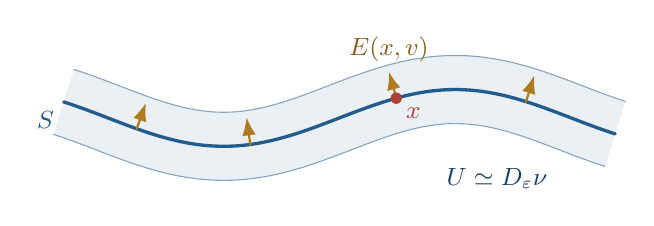
\begin{tikzpicture}[>=Latex,font=\small,line cap=round,scale=1.03,
 declare function={tubeheight(\t)=.35*sin(deg(1.1*\t))-.65;
 tubeslope(\t)=.385*cos(deg(1.1*\t));
 tubenx(\t)=-tubeslope(\t)/sqrt(1+tubeslope(\t)^2);
 tubeny(\t)=1/sqrt(1+tubeslope(\t)^2);}]
 \fill[manifoldblue!9]
  plot[domain=-3.4:3.4,samples=100,variable=\t]
   ({\t+.42*tubenx(\t)},{tubeheight(\t)+.42*tubeny(\t)})
  -- plot[domain=3.4:-3.4,samples=100,variable=\t]
   ({\t-.42*tubenx(\t)},{tubeheight(\t)-.42*tubeny(\t)}) -- cycle;
 \foreach \r in {-.42,.42}
  \draw[manifoldblue!55,thin]
   plot[domain=-3.4:3.4,samples=100,variable=\t]
    ({\t+\r*tubenx(\t)},{tubeheight(\t)+\r*tubeny(\t)});
 \draw[manifoldblue,very thick]
  plot[domain=-3.4:3.4,samples=100,variable=\t] (\t,{tubeheight(\t)});
 \foreach \t in {-2.5,-1.1,.7,2.3}
  \draw[->,manifoldgold!85!black,thick]
   (\t,{tubeheight(\t)}) -- ({\t+.34*tubenx(\t)},{tubeheight(\t)+.34*tubeny(\t)});
 \fill[manifoldred] (.7,{tubeheight(.7)}) circle (2pt)
   node[below right,manifoldred] {$x$};
 \node[above,manifoldgold!65!black]
   at ({.7+.34*tubenx(.7)},{tubeheight(.7)+.34*tubeny(.7)}) {$E(x,v)$};
 \node[below left,manifoldblue] at (-3.4,{tubeheight(-3.4)}) {$S$};
 \node[anchor=west,manifoldblue!70!black] at (1.2,-1.4)
   {$U\simeq D_\varepsilon\nu$};
\end{tikzpicture}
\caption{Otoczenie tubularne krzywej $S$ (ciemnoniebieska).
W metryce euklidesowej złote odcinki są prostopadłe do
stycznych krzywej, a $E(x,v)=x+v$ umieszcza ich końce
w jasnym pasie $U$. Brzegi pasa są odsunięte wzdłuż normalnych.}
\label{fig:tubularna-15}
\end{figure}

\begin{wniosek}[Cofnięcie otoczenia na podrozmaitość]
\label{cor:tuba-retrakcja}
W otoczeniu tubularnym istnieje gładkie
rzutowanie na podstawę
$r= \pr_S\circ E^{-1}:U\to S$.
Zanurzenie $S\hookrightarrow U$ jest
równoważnością homotopijną.
W szczególności $H_*(U;G)\cong H_*(S;G)$
dla dowolnej abelowej grupy współczynników $G$.
\end{wniosek}
\begin{proof}
Na dysku wiązki definiujemy
$h_t(x,v)=(x,(1-t)v)$, $0\leq t\leq1$.
Ponieważ $|(1-t)v|\leq|v|<\varepsilon(x)$,
jest to dobrze określona homotopia
od identyczności do rzutu na przekrój
zerowy, stale równa identyczności
na tym przekroju. Przeniesienie przez
$E$ daje silną retrakcję deformacyjną
$U$ na $S$. Niezmienniczość homotopijna
homologii była udowodniona w
Rozdziale~\ref{ch:homologia-przestrzeni}.
\end{proof}

\begin{przyklad}[Okrąg i sfera]
W $\R^2$ dla okręgu jednostkowego
$E(e^{i\theta},t)=(1+t)e^{i\theta}$
przy $|t|<1$. Obrazem jest pierścień
$0<|z|<2$, a $r(z)=z/|z|$.
W $\R^3$ analogicznie
$E(x,t)=(1+t)x$ dla $x\in S^2$;
mały dysk wiązki jest powłoką
sferyczną. Na wstędze Möbiusa
otoczenie środkowego okręgu
jest skręconą wiązką dyskową,
nie iloczynem $S^1\times(-\varepsilon,\varepsilon)$.
\end{przyklad}

\section{Obramowanie i dane potrzebne do chirurgii}
\label{sec:obramowanie-normalne}

\begin{definicja}[Obramowanie]
\index{obramowanie@Obramowanie}
\label{def:obramowanie-normalne}
\emph{Obramowaniem normalnym} (ang.\ \emph{framing})
zanurzenia $S^k\subset M^n$ nazywamy
uporządkowaną bazę gładkich przekrojów
$(n_1,\ldots,n_{n-k})$ wiązki $\nu(S,M)$
w każdym włóknie; równoważnie,
izomorfizm wiązek
$\nu(S,M)\cong S\times\R^{n-k}$.
\end{definicja}

Istnienie obramowania to silniejszy
warunek niż orientowalność wiązki:
obramowanie daje orientację, lecz
orientacja nie zawsze daje globalną
bazę. Po wyborze obramowania
twierdzenie tubularne przy zwartej
$S$ daje zanurzenie
\begin{equation}\label{eq:obramowany-dysk}
 S\times D^{\,n-k}_{\varepsilon}
 \longrightarrow M,\qquad
 (x,a_1,\ldots,a_{n-k})
 \longmapsto
 \exp_x\!\left(\sum_j a_jn_j(x)\right).
\end{equation}
Tutaj $D^r_\varepsilon=\{a\in\R^r:|a|\leq\varepsilon\}$
jest \emph{domkniętym} dyskiem, w odróżnieniu od otwartego
$D_\varepsilon\nu$ z twierdzenia tubularnego.
Istotnie, na zwartej $S$ istnieje $C>0$ takie, że
$|\sum a_jn_j(x)|_g\leq C|a|$. Wybieramy
$C\varepsilon$ ściśle mniejsze od jednolitego promienia
tubularnego. Wówczas wzór jest zanurzeniem nawet
na otoczeniu tego domkniętego dysku. Obramowanie
nie musi być ortonormalne.
Bez obramowania dziedziną jest
dysk \emph{wiązki} normalnej,
a nie globalny iloczyn.

\begin{przyklad}[Równik w sferze]
Włóżmy $S^k\subset S^n\subset\R^{n+1}$
jako punkty $(x,0)$ w rozkładzie
$\R^{n+1}=\R^{k+1}\oplus\R^{n-k}$.
Stałe wektory $e_{k+2},\ldots,e_{n+1}$
są w każdym punkcie $(x,0)$ styczne
do $S^n$, lecz prostopadłe do $T_xS^k$.
Tworzą więc obramowanie normalne.
W kontraście środkowy okrąg wstęgi
Möbiusa z Przykładu~\ref{prz:normalna-mobius}
nie dopuszcza nawet jednego
niezerowego normalnego przekroju.
\end{przyklad}

W teorii chirurgii wybiera się
często zanurzenie sfery wraz z
obramowaniem. Wzór~\eqref{eq:obramowany-dysk}
mówi wtedy dokładnie, \emph{które}
otoczenie $S^k\times D^{n-k}$
ma zostać usunięte. Różne obramowania
mogą dawać różne sklejenia po usunięciu;
samo wskazanie podrozmaitości
nie zawiera całej potrzebnej informacji.

\section{Kołnierz brzegu i podwojenie}
\label{sec:kolnierz-15}

\begin{definicja}[Kołnierz]
\index{kolnierz@Kołnierz}
Jeżeli $W$ jest rozmaitością z brzegiem,
\emph{kołnierzem brzegu} nazywamy zanurzenie
\[
 c:\partial W\times[0,1)\longrightarrow W,
 \qquad c(p,0)=p,
\]
którego obraz jest otwartym otoczeniem
$\partial W$ w $W$. Parametr $t$
oznacza ruch \emph{do wnętrza}.
\end{definicja}

\begin{twierdzenie}[Istnienie kołnierza]
\label{thm:kolnierz-15}
Każda gładka rozmaitość z brzegiem
ma kołnierz. Jeśli $\partial W$ jest
zwarty, kołnierz można przed
przeskalowaniem zapisać na
$\partial W\times[0,\varepsilon)$
z jedną stałą $\varepsilon>0$.
\end{twierdzenie}
\begin{proof}
W mapie półprzestrzennej
$(u^1,\ldots,u^{n-1},r)$, $r\geq0$,
wektor $\partial_r$ wskazuje do
wnętrza w punktach brzegu. Wybierzmy
lokalnie skończone pokrycie brzegu
takimi mapami i podział jedności
na niewielkim otoczeniu brzegu.
Ważona suma odpowiednich pól
$\partial_r$ jest gładkim polem
$V$, którego składowa skierowana
do wnętrza jest dodatnia:
każda dodatnia kombinacja
wektorów skierowanych do wnętrza
nadal jest skierowana do wnętrza.

Lokalny przepływ $\Phi_t$ tego pola przy brzegu
otrzymujemy, przedłużając jego współczynniki
w mapach półprzestrzennych przez $r=0$ i stosując
twierdzenie o równaniach różniczkowych. Jednoznaczność
spaja te lokalne rozwiązania, dopóki leżą w $W$.
Dla każdego $p\in\partial W$ istnieje otoczenie
$B_p$ w brzegu i czas $\tau_p>0$, dla których
$\Phi_t(q)$ jest określone w dziedzinie $V$
i leży we wnętrzu $W$ dla $q\in B_p$ i $0<t<\tau_p$.
Wynika to z dodatniej składowej pola w kierunku $r$
oraz ciągłej zależności rozwiązania od danych.

Za pomocą lokalnie skończonego podziału jedności
na brzegu wybieramy dodatnią gładką funkcję
$\varepsilon(p)$ tak małą, by te własności zachodziły
dla $0<t<\varepsilon(p)$. Dokładniej, dla podziału
$\{\chi_i\}$ podporządkowanego otoczeniom $B_i$
można wziąć $\varepsilon=\sum_i\chi_i\tau_i/2$:
przy ustalonym $p$ jest to średnia skończenie wielu
dopuszczalnych czasów, więc jest mniejsza od
największego z nich, także dopuszczalnego przy $p$.

Odwzorowanie $C(p,t)=\Phi_t(p)$ ma różniczkę
\[
 \dd C_{(p,t)}(u,a)=\dd\Phi_t{}_p(u+aV_p).
\]
Jest ona izomorfizmem: pole $V_p$ jest poprzeczne
do $T_p\partial W$, a różniczka lokalnego przepływu
jest odwracalna. Przy $t=0$ stosujemy twierdzenie
odwrotne w mapach półprzestrzennych; skierowanie
$V$ do wnętrza zapewnia właściwą stronę brzegu.
Tak $C$ jest lokalnym dyfeomorfizmem na dziedzinie
$\{(p,t):0\leq t<\varepsilon(p)\}$.

Globalna różnowartościowość wynika bezpośrednio
z jednoznaczności trajektorii. Jeżeli
$\Phi_t(p)=\Phi_s(q)$ i $t\geq s$, to cofając
obie trajektorie o czas $s$, dostajemy
$\Phi_{t-s}(p)=q$. Dla $t>s$ lewa strona
leży we wnętrzu, a $q$ na brzegu, co jest
niemożliwe. Zatem $t=s$ i $p=q$.
Różnowartościowy lokalny dyfeomorfizm $C$ jest
dyfeomorfizmem na otwarte otoczenie brzegu.
Wreszcie
\[
 c(p,s)=C(p,s\varepsilon(p)),\qquad 0\leq s<1,
\]
daje kołnierz z definicji. Przy zwartym brzegu
minimum dodatniej funkcji $\varepsilon$ jest dodatnie,
więc przed przeskalowaniem można użyć stałej szerokości.
\end{proof}

\begin{figure}[htbp]
\centering
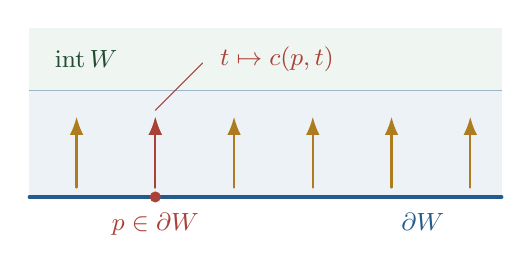
\begin{tikzpicture}[>=Latex,font=\small,line cap=round]
 \fill[manifoldblue!8] (-3,0) rectangle (3,1.35);
 \fill[manifoldgreen!8] (-3,1.35) rectangle (3,2.15);
 \draw[manifoldblue,very thick] (-3,0)--(3,0);
 \draw[manifoldblue!45] (-3,1.35)--(3,1.35);
 \foreach \x in {-2.4,-1.4,-.4,.6,1.6,2.6}
   \draw[->,manifoldgold!85!black,thick]
      (\x,0.12)--(\x,1.02);
 \fill[manifoldred] (-1.4,0) circle (2pt);
 \node[anchor=north,manifoldred] at (-1.4,-.08) {$p\in\partial W$};
 \node[anchor=west,manifoldblue] at (1.6,-.32) {$\partial W$};
 \draw[->,manifoldred,thick] (-1.4,.12)--(-1.4,1.02);
 \draw[manifoldred,thin] (-1.4,1.1)--(-.8,1.7);
 \node[anchor=west,manifoldred] at (-.7,1.75)
       {$t\mapsto c(p,t)$};
 \node[anchor=west,manifoldgreen!60!black] at (-2.8,1.75)
       {$\operatorname{int}W$};
\end{tikzpicture}
\caption{Kołnierz zamienia całe otoczenie brzegu
w produkt $\partial W\times[0,1)$.
Współrzędna $t$ rośnie do wnętrza rozmaitości.}
\label{fig:kolnierz-15}
\end{figure}

\begin{przyklad}[Dysk i walec]
Dla dysku jednostkowego $D^2$
kołnierz można zapisać jako
$c(p,t)=(1-t)p$ dla $p\in S^1$
i $0\leq t<\varepsilon<1$.
Dla $W=S^1\times[0,1]$ brzeg
ma dwie składowe: przy $0$
parametr idzie w górę, a przy
$1$ w dół. Jest to konkretny
powód, dla którego orientacje
dwóch składowych brzegu walca
są przeciwne.
\end{przyklad}

\begin{wniosek}[Podwojenie rozmaitości]
\label{cor:podwojenie-15}
Dwie kopie $W_+$ i $W_-$ rozmaitości
z brzegiem można skleić wzdłuż
identyczności $\partial W$ tak,
aby otrzymać gładką rozmaitość
bez brzegu
$DW=W_+\cup_{\partial W}W_-$.
Jeżeli $W$ jest zwarta, $DW$
też jest zwarta.
\end{wniosek}
\begin{proof}
Poza brzegiem korzystamy z
istniejących map gładkich obu kopii.
W pobliżu sklejonego brzegu
używamy kołnierzy i współrzędnej
$s\in(-1,1)$: dla $s\geq0$
punkt $(p,s)$ oznacza $c_+(p,s)$,
a dla $s\leq0$ oznacza
$c_-(p,-s)$. Wspólne przejścia
między takimi mapami mają postać
$(p,s)\mapsto(\psi\circ\varphi^{-1}(p),s)$,
więc są gładkie. Z kolei przejścia
do map pochodzących z wnętrza
odbywają się dla $s\ne0$ i także
są gładkie. Otrzymujemy atlas
bez półprzestrzennych punktów
brzegowych. Sprawdźmy też warunki topologiczne.
Różne punkty szwu rozdzielamy rozłącznymi otoczeniami
w $\partial W$ i ich kołnierzami. Punkt wnętrza
można oddzielić od szwu, zmniejszając otoczenie
tak, by jego domknięcie nie dochodziło do brzegu;
następnie dobieramy odpowiednio małe otoczenie
drugiego punktu. Punkty wnętrz rozdziela własność
Hausdorffa w kopiach $W$. Iloraz jest więc Hausdorffa.
Przeliczalne atlasy obu wnętrz i brzegu wraz
z przedziałami o wymiernych końcach dają przeliczalną
bazę ilorazu. Jeśli $W$ jest zwarta, ciągły obraz
zwartej sumy rozłącznej $W_+\sqcup W_-$ jest zwarty.
\end{proof}

\section{Izotopie i zgodność otoczeń}
\label{sec:izotopie-otoczen-15}

Izotopia to gładka rodzina zanurzeń
$i_t:S\hookrightarrow M$, $0\leq t\leq1$.
Rozdział~\ref{ch:pola} zawiera
już dowód twierdzenia o rozszerzeniu
izotopii~\ref{thm:rozszerzenie-izotopii}
dla zwartej $S$ bez brzegu:
istnieje izotopia otoczenia
$h_t:M\to M$ z $h_0=\id$
i $h_t\circ i_0=i_t$.
Nie powtarzamy tamtego dowodu;
wykorzystamy jego wnioski geometryczne.

\begin{wniosek}[Otoczenia i dopełnienia izotopijnych zanurzeń]
\label{cor:izotopia-dopelnienia}
Jeśli $S$ jest zwarta bez brzegu,
a $i_t:S\hookrightarrow M$ jest
gładką izotopią, to
\[
 M\setminus i_0(S)\cong M\setminus i_1(S)
 \quad\text{oraz}\quad
 \nu(i_0(S),M)\cong \nu(i_1(S),M)
\]
jako odpowiednio rozmaitości
i wiązki nad $S$. Można wybrać
otoczenia tubularne obu obrazów
odpowiadające sobie przez $h_1$.
\end{wniosek}
\begin{proof}
Twierdzenie~\ref{thm:rozszerzenie-izotopii}
daje dyfeomorfizm $h_1$ z
$h_1(i_0(S))=i_1(S)$.
Jego ograniczenie do dopełnień
ma odwrotność $h_1^{-1}$.
Różniczka $\dd h_1$ wysyła
$T(i_0(S))$ na $T(i_1(S))$,
a więc przechodzi do
izomorfizmu ilorazów
$TM|_{i_0(S)}/T(i_0(S))
\to TM|_{i_1(S)}/T(i_1(S))$.
Jeśli $E_0:D_\varepsilon\nu_0\to U_0$
jest otoczeniem tubularnym,
to złożenie $h_1\circ E_0$
opisuje otoczenie $h_1(U_0)$
przez tę samą wiązkę; po
uzyskanym izomorfizmie $\nu_0\cong\nu_1$
jest to opis przez $\nu_1$. Precyzyjniej, jeśli $A$
oznacza ten izomorfizm, nowym odwzorowaniem tubularnym jest
$E_1=h_1\circ E_0\circ A^{-1}$. Nie musi ono być
odwzorowaniem wykładniczym dla początkowej metryki na $M$.
Jest nim dla metryki przeniesionej przez $h_1$,
ponieważ izometria przenosi geodezyjne i normalne.
\end{proof}

\begin{uwaga}[Co właściwie jest zachowane?]
Wniosek nie mówi, że dowolne dwa
zanurzenia tej samej abstrakcyjnej
sfery mają dyfeomorficzne dopełnienia.
Wymagana jest \emph{izotopia zanurzeń}
w ustalonym $M$. W szczególności
różne węzły w $\R^3$ mogą mieć
różne dopełnienia; nie należy
utożsamiać deformacji abstrakcyjnego
okręgu z izotopią w przestrzeni
otaczającej.
\end{uwaga}

Kołnierze tej samej zwartej
składowej brzegu można także
porównywać: z kołnierza $c_j$
otrzymujemy pole
$(c_j)_*(\partial_t)$ w pobliżu
brzegu. Oba pola są skierowane
do wnętrza. Ich interpolacja
$(1-s)V_0+sV_1$ nadal jest
skierowana do wnętrza;
jej przepływ daje, po wyborze
wspólnego małego czasu na
zwartym brzegu, rodzinę
kołnierzy łączącą oba opisy.
Oznaczmy tę rodzinę przez $C_s(p,t)$. Aby otrzymać
dyfeomorfizm, a nie tylko rodzinę opisów, definiujemy
w jej obrazie zależne od $s$ pole
$Y_s(C_s(p,t))=\partial_s C_s(p,t)$.
Ponieważ $C_s(p,0)=p$, pole to znika na brzegu.
Wybieramy gładkie odcięcie równe $1$ na mniejszym
kołnierzu i równe $0$ przed zewnętrznym końcem większego.
Zwartość brzegu i przedziału parametrów pozwala dobrać
wspólną szerokość i zwarty nośnik dla całej rodziny.
Przepływ powstałego pola jest izotopią $H_s$ rozmaitości
$W$, ustaloną na brzegu; jednoznaczność rozwiązań daje
$H_s(C_0(p,t))=C_s(p,t)$ w mniejszym kołnierzu.
Stosując $H_1$ na obu kopiach $W$, otrzymujemy
dyfeomorfizm odpowiednich podwojeń: przy szwie
współrzędne $(p,\text{czas ze znakiem})$ są zachowane.
Wyjaśnia to niezależność gładkiego podwojenia, z dokładnością
do dyfeomorfizmu, od wyboru kołnierza przy zwartym brzegu.

\section{Funkcje wyczerpujące i regularne poziomice}
\label{sec:wyczerpujace-15}

\begin{definicja}[Funkcja wyczerpująca]
\index{funkcja wyczerpujaca@Funkcja wyczerpująca}
\label{def:wyczerpujaca-15}
Funkcja ciągła $\rho:M\to[0,\infty)$ jest
\emph{wyczerpująca}, jeśli jest właściwa,
czyli $\rho^{-1}([0,a])$ jest zwarty
dla każdego $a\geq0$.
Nie wymaga się, by $\rho$ była
funkcją Morse'a.
\end{definicja}

\begin{twierdzenie}[Istnienie gładkiego wyczerpania]
\label{thm:wyczerpanie-15}
Każda rozmaitość gładka z przeliczalną
bazą, również z brzegiem, ma gładką
nieujemną funkcję wyczerpującą.
Na rozmaitości bez brzegu istnieje
ciąg dowolnie dużych wartości regularnych
$a_j\to\infty$; zbiory
$\rho^{-1}((-\infty,a_j])$ są wtedy
zwartymi rozmaitościami z gładkim
brzegiem $\rho^{-1}(a_j)$.
\end{twierdzenie}
\begin{proof}
Z lokalnej zwartości i przeliczalnej
bazy budujemy zwarte zbiory
$K_1\subset\operatorname{int}K_2
\subset K_2\subset\operatorname{int}K_3
\subset\cdots$ o sumie równej $M$.
W tym celu wybieramy przeliczalne pokrycie
$\{B_j\}$ zbiorami otwartymi o zwartych domknięciach.
Mając $K_j$, pokrywamy zwarty zbiór
$K_j\cup\overline{B_{j+1}}$ skończenie wieloma
względnie zwartymi otwartymi otoczeniami i za
$K_{j+1}$ bierzemy sumę ich domknięć. Zaczynamy od
$K_1\supset\overline{B_1}$; konstrukcja zapewnia
zarówno zawieranie we wnętrzach, jak i wyczerpanie $M$.

Dla każdego $j$ skonstruujmy
gładką $\psi_j:M\to[0,1]$
równą $0$ w otoczeniu $K_j$
i równą $1$ poza
$\operatorname{int}K_{j+1}$.
Istnienie wynika z gładkiego
lematu o funkcji odcinającej:
zbiory $K_j$ i
$M\setminus\operatorname{int}K_{j+1}$
są rozłączne i domknięte, a
lokalnie skończony podział
jedności oddziela je gładko.
Połóżmy
\[
 \rho(x)=\sum_{j=1}^{\infty}\psi_j(x).
\]
Wybierzmy $m$ tak, by $x\in\operatorname{int}K_m$.
Wszystkie $\psi_j$ dla $j\geq m$ są równe zeru
na tym samym otoczeniu $\operatorname{int}K_m$;
suma jest lokalnie skończona,
zatem $\rho$ jest gładka.
Jeśli $x\notin K_{N+1}$,
to dla $j\leq N$ mamy
$x\notin\operatorname{int}K_{j+1}$,
więc $\psi_j(x)=1$ i $\rho(x)\geq N$.
Stąd $\{\rho\leq a\}$ zawiera się
w $K_{N+1}$ dla $N>a$.
Jest domknięty, zatem zwarty;
to dowodzi właściwości.

Dla rozmaitości bez brzegu
twierdzenie Sarda~\ref{thm:sard}
daje wartości regularne poza
zbiorem miary zero. W każdym
przedziale $(j,j+1)$ można
wybrać wartość regularną $a_j$.
W pobliżu każdego punktu jej
poziomicy twierdzenie o submersji
zapisuje $\rho$ jako jedną
ze współrzędnych, więc podpoziomica
ma lokalny model półprzestrzeni.
Jej brzeg jest właśnie
$\rho^{-1}(a_j)$.
\end{proof}

\begin{twierdzenie}[Właściwa funkcja Morse'a]
\label{thm:wlasciwa-morse-15}
Na każdej gładkiej rozmaitości bez brzegu
istnieje nieujemna właściwa funkcja Morse'a $f:M\to\R$.
Każda jej podpoziomica $\{f\leq a\}$ jest zwarta.
Jej punkty krytyczne mogą być nieskończenie liczne,
ale w każdej podpoziomicy jest ich skończenie wiele.
\end{twierdzenie}
\begin{proof}
Zaczynamy od gładkiej właściwej
funkcji $\rho$ z
Twierdzenia~\ref{thm:wyczerpanie-15}.
Wybierzmy zwarte
$K_1\subset\operatorname{int}K_2
\subset K_2\subset\cdots$
o sumie $M$; dla wygody
$K_0=\varnothing$. Połóżmy $f_0=\rho$.
Skonstruujemy funkcje
$f_j=f_{j-1}+h_j$ tak, aby $f_j$
była Morse'a na otoczeniu $K_j$,
a przyszłe poprawki nie niszczyły
tej własności.

Pokryjmy $K_j$ skończoną liczbą
mniejszych obszarów map. W większych
obszarach wybierzmy funkcje
odcinające $\beta_i$, równe $1$
na mniejszych. Funkcje
$\beta_i x_i^1,\ldots,\beta_i x_i^n$,
przedłużone przez zero, mają
różniczki rozpinające $T_x^*M$
dla każdego $x\in K_j$:
w jednym z mniejszych obszarów
są po prostu współrzędnymi.
Zatem dla rodziny
\[
 f_{j,a}=f_{j-1}
       +\sum_{i,\ell}a_{i\ell}\beta_i x_i^\ell
\]
parametryczna różniczka
$(x,a)\mapsto\dd f_{j,a}(x)$
jest transwersalna do przekroju
zerowego nad otoczeniem $K_j$.
Dowód transwersalności
parametrycznej z
Twierdzenia~\ref{thm:transwersalnosc-param}
pozwala wybrać \emph{dowolnie
małe} parametry $a$, dla których
$f_{j,a}$ jest Morse'a na
otoczeniu $K_j$. Niech $h_j$
będzie otrzymaną poprawką.
Jest sumą skończenie wielu
funkcji o zwartych nośnikach.

Uściślijmy wybór wielkości poprawek. Ustalmy
metrykę riemannowską i jej połączenie $\nabla$ oraz normy
\[
 \|h\|_{C^r(K)}=\max_{0\leq\ell\leq r}
       \sup_{x\in K}|\nabla^\ell h(x)|.
\]
Na zbiorach zwartych są one równoważne normom
w skończonych układach map; rosną wraz z $K$ i $r$.
Normy na pustym $K_0$ przyjmujemy równe zeru.
Skoro $f_i$ jest Morse'a na
otoczeniu zwartego $K_i$,
istnieje $\eta_i>0$ takie,
że perturbacja o normie
$C^2(K_i)$ mniejszej od
$\eta_i$ zachowuje
niezdegenerowanie wszystkich
punktów krytycznych na $K_i$.
Wynika to z otwartości
transwersalności $\dd f_i$
do przekroju zerowego
na zwartym zbiorze.
W kroku $j$ wybieramy małe
parametry tak, aby dodatkowo
\[
 \|h_j\|_\infty<2^{-j},\qquad
 \|h_j\|_{C^j(K_{j-1})}<2^{-j},\qquad
 \|h_j\|_{C^2(K_i)}
          <2^{-j}\eta_i\quad(i<j).
\]
Każdy krok narzuca tylko
skończenie wiele warunków
otwartych przy $a=0$,
więc można je pogodzić
z wyborem dobrego $a$.

Szereg $f=\rho+\sum_{j\geq1}h_j$
zbiega gładko na każdym zwartym
zbiorze: dla ustalonego $K_i$
i rzędu pochodnej $r$ wszystkie
wyrazy o $j>\max(i,r)$ mają normę
$C^r(K_i)$ ograniczoną przez
$2^{-j}$. Ponadto
$|f-\rho|\leq\sum_j2^{-j}=1$.
Zatem przeciwobraz zwartego
przedziału $[-A,A]$ przez $f$
leży w zwartej podpoziomicy
$\{\rho\leq A+1\}$ i jest
domknięty, czyli zwarty.
Funkcja $f$ jest właściwa.
Na $K_i$ różnica $f-f_i$
ma normę $C^2$ mniejszą
od $\eta_i\sum_{j>i}2^{-j}
<\eta_i$; funkcja $f$
pozostaje tam Morse'a.
Ponieważ $K_i$ wyczerpują
$M$, jest Morse'a wszędzie. Ponieważ $f\geq-1$,
zastępujemy ją na końcu przez $f+1$. Otrzymana funkcja
jest nieujemna, nadal właściwa i Morse'a, a jej
podpoziomice są przeciwobrazami zwartych przedziałów.
Jej punkty krytyczne są izolowane;
ich zbiór w zwartej podpoziomicy
jest domknięty i dlatego skończony.
\end{proof}

\begin{stwierdzenie}[Metryka zupełna]
\label{prop:metryka-zupelna-wyczerpanie}
Każda rozmaitość gładka bez brzegu
ma zupełną metrykę riemannowską.
Ten sam wniosek w sensie zupełnej
odległości metrycznej zachodzi
dla rozmaitości z brzegiem.
\end{stwierdzenie}
\begin{proof}
Wybierzmy dowolną metrykę $g$
i gładkie właściwe $\rho$
z Twierdzenia~\ref{thm:wyczerpanie-15}.
Niech
$\lambda=\sqrt{1+|\nabla_g\rho|_g^2}$
i $g'=\lambda^2g$.
Ponieważ
$|\nabla_{g'}\rho|_{g'}
=|\nabla_g\rho|_g/\lambda\leq1$,
całkowanie po dowolnej kawałkami
gładkiej krzywej $\gamma$ daje
\[
 |\rho(\gamma(1))-\rho(\gamma(0))|
 \leq L_{g'}(\gamma).
\]
Po wzięciu kresu dolnego długości
$|\rho(x)-\rho(y)|\leq d_{g'}(x,y)$.
Niech $(x_j)$ będzie ciągiem Cauchy'ego
w odległości $d_{g'}$. Jego odległości
od ustalonego $x_1$ są ograniczone,
więc wartości $\rho(x_j)$ też są
ograniczone. Cały ciąg leży
w pewnej zwartej podpoziomicy
$\{\rho\leq A\}$, zatem ma podciąg
zbieżny. Ponieważ $(x_j)$ jest
Cauchy'ego i topologia $d_{g'}$
zgadza się z topologią rozmaitości,
cały ciąg zbiega. Ten sam argument
dla krzywych leżących w rozmaitości
z brzegiem daje jej zupełność
jako przestrzeni metrycznej. Zgodność topologii
przy brzegu wynika z lokalnego porównania metryki
z euklidesową w mniejszych wypukłych półkulach map.
Przy niespójnym $M$ zupełność riemannowską rozumiemy
składowa po składowej, ponieważ między różnymi składowymi
nie ma krzywych. Jeśli potrzebna jest jedna skończona
odległość na całym $M$, bierzemy $\min(d_{g'},1)$
na każdej składowej i odległość $1$ pomiędzy nimi.
Jest ona zupełna i wyznacza topologię $M$.
\end{proof}

\begin{przyklad}
Na $\R^n$ funkcja $\rho(x)=|x|^2$
jest wyczerpująca, bo
$\{\rho\leq a\}$ to domknięta
kula promienia $\sqrt a$.
Na otwartym przedziale $(0,1)$
działa na przykład
$\rho(x)=x^{-2}+(1-x)^{-2}$:
rośnie bez ograniczenia przy
obu końcach. Funkcja $x^2$
na $(0,1)$ nie jest właściwa:
punkty mogą zbliżać się do
brzegu $0$ przy ograniczonych
wartościach $x^2$.
\end{przyklad}

\begin{twierdzenie}[Pas bez punktów krytycznych jest produktem]
\label{thm:pas-bez-krytycznych-15}
Niech $M$ będzie rozmaitością bez brzegu,
$f:M\to\R$ gładką funkcją
i właściwą, a $a<b$. Załóżmy,
że $f$ nie ma punktów krytycznych
w $f^{-1}([a,b])$. Wtedy
\[
 f^{-1}([a,b])\cong f^{-1}(a)\times[a,b],
 \qquad f\ \text{odpowiada rzutowi na }[a,b].
\]
Jeżeli poziomica $f^{-1}(a)$ jest pusta,
obie strony są puste.
\end{twierdzenie}
\begin{proof}
Pas $K=f^{-1}([a,b])$ jest zwarty,
bo $f$ jest właściwa. Dla $K=\varnothing$ teza
jest natychmiastowa. W przeciwnym razie na nim
$\nabla f\ne0$, więc pole
\[
 X=\frac{\nabla f}{|\nabla f|^2}
\]
jest określone w otoczeniu $K$.
Wybierzmy gładką funkcję
odcinającą $\chi$ o zwartym
nośniku w tym otoczeniu,
równą $1$ na $K$, i zastąpmy
$X$ przez globalne, zwartego
nośnika pole $\chi X$.
Jego przepływ $\Phi_t$
istnieje dla wszystkich
$t\in\R$ dzięki zwartości
nośnika. Dopóki trajektoria
pozostaje w $K$, mamy
\[
 \frac{\dd}{\dd t}f(\Phi_t(x))
 =\dd f_{\Phi_t(x)}(X)
 =g(\nabla f,\nabla f)/|\nabla f|^2=1.
\]
Startując z $x\in f^{-1}(a)$,
trajektoria nie może opuścić
$K$ przed czasem $b-a$:
wcześniejsze opuszczenie
wymagałoby wartości $f$
poza $[a,b]$, podczas gdy
na każdym wcześniejszym
odcinku $f(\Phi_t(x))=a+t$.
Zatem
$\Psi(x,s)=\Phi_{s-a}(x)$
dla $s\in[a,b]$ jest
dobrze określona i ma
$f(\Psi(x,s))=s$.
Analogicznie trajektoria startująca z $y\in K$
pozostaje w $K$ dla $a-f(y)\leq t\leq0$ i spełnia
$f(\Phi_t(y))=f(y)+t$. Dochodzi więc do poziomicy $a$;
jeśli ta jest pusta, nie mogło być żadnego $y\in K$.
Własność grupowa przepływu pokazuje, że odwrotnością
$\Psi$ jest
\[
 y\longmapsto
       \bigl(\Phi_{a-f(y)}(y),\,f(y)\bigr).
\]
Przepływ i $f$ są gładkie,
więc oba odwzorowania są gładkie,
także w mapach półprzestrzennych
przy $a$ i $b$. To daje
żądaną identyfikację.
\end{proof}

\begin{figure}[htbp]
\centering
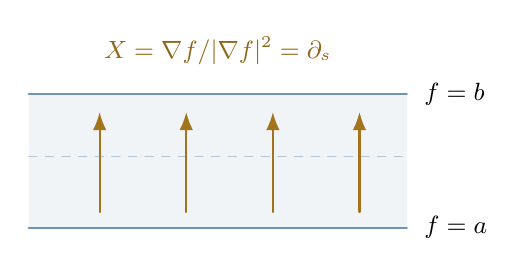
\begin{tikzpicture}[>=Latex,font=\small,line cap=round]
 \fill[manifoldblue!7] (-2.4,.55) rectangle (2.4,2.25);
 \draw[manifoldblue!65,thick] (-2.4,.55)--(2.4,.55);
 \draw[manifoldblue!65,thick] (-2.4,2.25)--(2.4,2.25);
 \draw[manifoldblue!35,dashed] (-2.4,1.45)--(2.4,1.45);
 \foreach \x in {-1.5,-.4,.7,1.8}
  \draw[->,manifoldgold!80!black,thick] (\x,.75)--(\x,2.02);
 \node[anchor=west] at (2.5,.55) {$f=a$};
 \node[anchor=west] at (2.5,2.25) {$f=b$};
 \node[above,manifoldgold!70!black] at (0,2.5)
       {$X=\nabla f/|\nabla f|^2=\partial_s$};
\end{tikzpicture}
\caption{Przepływ pola $X$ przenosi punkt poziomicy
$f=a$ na poziomicę $f=a+t$. Gdy w zwartym pasie
nie ma punktów krytycznych, wszystkie poziomice
składają się w produkt. Rysunek przedstawia współrzędne
produktowe $(x,s)$ wyznaczone przez przepływ; w nich $f=s$.}
\label{fig:pas-bez-krytycznych-15}
\end{figure}

\begin{uwaga}[Związek z późniejszą teorią Morse'a]
Jeśli $\rho$ jest właściwa,
zmiany topologii jej podpoziomic
mogą zachodzić tylko przy
przechodzeniu przez wartości
krytyczne: pomiędzy nimi
Twierdzenie~\ref{thm:pas-bez-krytycznych-15}
identyfikuje pas z produktem.
Teoria Morse'a opisze
konkretną zmianę przy
niezdegenerowanym punkcie
krytycznym. Tu potrzebowaliśmy
jedynie pojęcia punktu
krytycznego z Rozdziału~\ref{ch:sard-transwersalnosc}.
\end{uwaga}

\par\smallskip
{\footnotesize\noindent\emph{Dalsza lektura:}
\href{https://ocw.mit.edu/courses/18-965-geometry-of-manifolds-fall-2004/d0598b3b5ced2d2d0a9884ee14abeae3_lecture21_22.pdf}{wykłady MIT o mocnym twierdzeniu Whitneya},
\href{https://arxiv.org/pdf/1907.10297}{omówienie dysku Whitneya w wykładach Benedettiego},
\href{https://ocw.mit.edu/courses/18-966-geometry-of-manifolds-spring-2007/238234d53148cb71c5880e529a96c73f_lect05.pdf}{wykład MIT o otoczeniach tubularnych}.\par}

\chapter{Przecięcia, dualność i klasy charakterystyczne}
\label{ch:przeciecia-dualnosc-klasy}
\index{dualnosc Poincarego@Dualność Poincarégo}

Otoczenie tubularne z Rozdziału~\ref{ch:wlozenia-otoczenia}
pozwala odróżnić ruch \emph{wzdłuż} podrozmaitości
od ruchu \emph{poprzecznego}. Teraz przypiszemy
przecięciom liczby, a wiązkom -- klasy kohomologii.
W ten sposób geometryczne dane zanurzenia stają się
niezmiennikami, które można obliczać i porównywać.
To przygotowanie do teorii Morse'a, Smale'a i chirurgii;
w końcowej sekcji wykonamy też prostą operację
wycinania i sklejania rozmaitości.

Przez \emph{zamkniętą rozmaitość} rozumiemy w tym
rozdziale rozmaitość zwartą bez brzegu. W dowodzie
komórkowym będziemy używać triangulacji gładkiej
rozmaitości. Jej istnienie jest osobnym, głębszym
twierdzeniem o triangulacji; opisujemy dokładnie
argument dualności \emph{po} wybraniu takiej
triangulacji. Rozróżnienie tych dwóch kroków
zapobiega ukryciu twierdzenia o triangulacji
w rysunku.

\section{Kochainy symplicjalne i iloczyn kubkowy}
\label{sec:kubek-16}

Kompleksy łańcuchowe i ich duale poznaliśmy
w Rozdziałach~\ref{ch:algebra-homologiczna}
i~\ref{ch:homologia-przestrzeni}. Dla
skończonej triangulacji $K$ i ciała $\mathbb F$
zapisujemy precyzyjnie
\[
 C^k(K;\mathbb F)
   =\operatorname{Hom}_{\mathbb F}
       (C_k(K;\mathbb F),\mathbb F),
 \qquad
 (\dd\varphi)(c)=\varphi(\partial c).
\]
\emph{Kochain} $\varphi\in C^k$ jest więc
funkcją liniową \emph{na łańcuchach} stopnia $k$.
Nie jest kolejnym rodzajem sympleksu:
przypisuje każdemu łańcuchowi liczbę z
$\mathbb F$. To polska nazwa angielskiego
\emph{cochain}; łańcuch należy do $C_k$,
a kochain do przestrzeni dualnej $C^k$.
Znak $\partial$ pozostaje zarezerwowany
dla łańcuchów, a $\dd$ dla kochainów.
Równość $\dd^2=0$ wynika od razu z
$\partial^2=0$. Klasa w $H^k$ to
funkcja na cyklach, która nie zmienia
się po dodaniu brzegu. Nad ciałem
$H^k(K;\mathbb F)\cong
\operatorname{Hom}_{\mathbb F}(H_k(K;\mathbb F),\mathbb F)$:
można wybrać uzupełnienia baz jąder
i obrazów i zdualizować powstały
rozkład. Nad $\Z$ analogiczne zdanie
wymaga poprawki $\operatorname{Ext}$,
co było omawiane przy zmianie
współczynników w Rozdziale~\ref{ch:algebra-homologiczna}.
Pracę nad ciałem rozpoczniemy tu dlatego,
że łatwiej zobaczyć parowanie;
dualność Poincarégo ma również
wersję całkowitą.

\begin{definicja}[Iloczyn kubkowy]
\index{iloczyn kubkowy@Iloczyn kubkowy}
\label{def:kubek-16}
Ustalmy porządek wierzchołków $K$ i przemienny
pierścień współczynników $R$ (w szczególności $\Z$ lub ciało).
Dla $\alpha\in C^p(K;R)$ i $\beta\in C^q(K;R)$ definiujemy
na sympleksach o wierzchołkach zapisanych rosnąco
\[
(\alpha\smile\beta)
 [v_0,\ldots,v_{p+q}]
=\alpha[v_0,\ldots,v_p]\,
 \beta[v_p,\ldots,v_{p+q}].
\]
Na przeciwnie zorientowanym sympleksie przedłużamy ten
wzór liniowo ze znakiem. Obie ściany dzielą wierzchołek $v_p$.
Po przejściu do kohomologii otrzymamy
iloczyn $H^p\times H^q\to H^{p+q}$.
\end{definicja}

\begin{stwierdzenie}[Reguła Leibniza]
\label{prop:kubek-leibniz-16}
Dla kochainów zachodzi
\[
 \dd(\alpha\smile\beta)
 =(\dd\alpha)\smile\beta
       +(-1)^p\alpha\smile(\dd\beta).
\]
Zatem iloczyn klas kohomologii jest
dobrze określony; jest łączny.
\end{stwierdzenie}
\begin{proof}
Obliczamy prawą stronę na $[v_0,\ldots,v_{p+q+1}]$.
W $(\dd\alpha)\smile\beta$ wyrazy z usunięciem
$v_i$ dla $0\leq i\leq p$ odpowiadają dokładnie
tym samym wyrazom w $\dd(\alpha\smile\beta)$.
W $(-1)^p\alpha\smile\dd\beta$ odpowiadają im
pozostałe wyrazy, o indeksach $p+1\leq i\leq p+q+1$.
Na prawej stronie są ponadto dwa dodatkowe wyrazy:
\[
 \bigl((-1)^{p+1}+(-1)^p\bigr)
 \alpha[v_0,\ldots,v_p]\,
 \beta[v_{p+1},\ldots,v_{p+q+1}]=0.
\]
Pochodzą one odpowiednio z ostatniej ściany
$\dd\alpha$ i pierwszej ściany $\dd\beta$.
To one się znoszą; żaden wyraz lewego kobrzegu
nie zostaje usunięty. Otrzymujemy regułę Leibniza.
Jeśli $\dd\alpha=\dd\beta=0$,
iloczyn jest kocyklem.
Jeśli $\alpha$ zastąpimy przez
$\alpha+\dd\gamma$, to zmiana
iloczynu wynosi
$\dd(\gamma\smile\beta)$
przy zamkniętej $\beta$;
przy zmianie $\beta$ na $\beta+\dd\eta$ różnica
wynosi $(-1)^p\dd(\alpha\smile\eta)$ przy zamkniętej $\alpha$.
Łączność widać bezpośrednio:
obie iteracje na sympleksie
stopnia $p+q+r$ dają iloczyn
wartości na trzech kolejnych
ścianach
$[v_0,\ldots,v_p]$,
$[v_p,\ldots,v_{p+q}]$ i
$[v_{p+q},\ldots,v_{p+q+r}]$.
\end{proof}

\begin{stwierdzenie}[Przemienność z właściwym znakiem]
\label{prop:kubek-graded-16}
W kohomologii
$\alpha\smile\beta
=(-1)^{pq}\beta\smile\alpha$
dla $\alpha\in H^p$,
$\beta\in H^q$.
\end{stwierdzenie}
\begin{proof}
Pracujemy najpierw nad $\Z$ i oznaczamy $C=C_*(K;\Z)$.
Na kompleksie tensorowym przyjmujemy
$\partial(a\otimes b)=\partial a\otimes b+(-1)^{|a|}a\otimes\partial b$.
Odwzorowanie Alexandera--Whitneya ma postać
\[
 A[v_0,\ldots,v_m]
 =\sum_{j=0}^m[v_0,\ldots,v_j]\otimes[v_j,\ldots,v_m].
\]
Jest odwzorowaniem łańcuchowym: po rozpisaniu brzegów
wyrazy wewnętrzne przy miejscu podziału znoszą się
tak jak w poprzednim dowodzie. Również
$T(a\otimes b)=(-1)^{|a||b|}b\otimes a$
jest odwzorowaniem łańcuchowym.

Skonstruujemy homotopię $H$ między $A$ i $TA$.
Dla wierzchołków oba odwzorowania są równe, więc
kładziemy $H=0$ w stopniu zero. Jeżeli $H$ jest
już określone na ścianach sympleksu $\sigma^m$,
łańcuch
\[
 z=TA(\sigma)-A(\sigma)-H(\partial\sigma)
\]
jest cyklem: stosujemy $\partial$, korzystamy
z łańcuchowości obu odwzorowań i założenia indukcyjnego.
Cały $z$ leży w $C_*(\sigma)\otimes C_*(\sigma)$.
Ten kompleks ma zerową homologię w dodatnich stopniach:
stożkowanie sympleksu do jego wierzchołka jest
ściągnięciem łańcuchowym do $\Z$ w stopniu zero,
a ze ściągnięć obu czynników konstruujemy ściągnięcie
ich iloczynu tensorowego.
Możemy więc wybrać $H(\sigma)$ z $\partial H(\sigma)=z$.
Indukcja daje $\partial H+H\partial=TA-A$.

Dla kocykli $\alpha,\beta$ kochain
$\alpha\otimes\beta$ znika na brzegach kompleksu
tensorowego. Po ewaluacji ostatniej tożsamości
otrzymujemy, że
$(-1)^{pq}\beta\smile\alpha-\alpha\smile\beta$
jest kobrzegiem kochainu $(\alpha\otimes\beta)H$.
Dowód działa po zmianie współczynników na $R$.
Ta sama indukcja w ściągalnych nośnikach pokazuje
niezależność od porządku wierzchołków i wyboru
przybliżenia przekątnej. W połączeniu z aproksymacją
symplicjalną daje naturalność iloczynu w kohomologii.
\end{proof}

W przeciwieństwie do samego wymiaru
grup $H^k$, iloczyn kubkowy pamięta,
\emph{jak} różne cykle są względem siebie
położone. Ta dodatkowa informacja
wyjaśni później liczby przecięcia.
Oznaczenie $\smile$ odróżnia
iloczyn kochainów od iloczynu
zewnętrznego form $\wedge$ z
Rozdziału~\ref{ch:formy-de-rham}.

\begin{definicja}[Iloczyn kapowy i konwencja znaków]
\index{iloczyn kapowy i konwencja znakow@Iloczyn kapowy i konwencja znaków}
\label{def:kapowy-16}
Dla $m$-sympleksu $c=[v_0,\ldots,v_m]$ i kochainu
$\alpha$ stopnia $k\leq m$ kładziemy
\[
 c\frown\alpha=\alpha[v_0,\ldots,v_k]\,[v_k,\ldots,v_m].
\]
Wzór przedłużamy liniowo. Możemy wziąć całkowity łańcuch
i kochain o wartościach w dowolnej grupie abelowej $G$;
wtedy wynik jest łańcuchem z $G$. Bezpośrednie rozpisanie
ścian (z tym samym skróceniem dwóch wyrazów przy podziale)
daje
\begin{equation}\label{eq:kapowy-brzeg-16}
 \partial(c\frown\alpha)=(-1)^k
  \bigl((\partial c)\frown\alpha-c\frown\dd\alpha\bigr).
\end{equation}
Dlatego cykl i kocykl wyznaczają klasę homologii,
niezależną od reprezentantów. Dla współczynników w $R$
mamy ponadto, prosto ze wzorów na ściany,
\[
 \langle\beta,c\frown\alpha\rangle
 =\langle\alpha\smile\beta,c\rangle.
\]
Ta kolejność czynników będzie obowiązywała w całym rozdziale.
\end{definicja}

\section{Orientacja jako klasa homologii}
\label{sec:klasa-fundamentalna-16}

W Stwierdzeniu~\ref{prop:lokalna-homologia}
ustaliliśmy, że
$H_n(M,M\setminus\{x\};\Z)\cong\Z$.
Orientacja oznacza spójny wybór
generatorów tych lokalnych grup.
Teraz skleimy je w jedną klasę
globalną.

\begin{twierdzenie}[Klasa fundamentalna]
\label{thm:klasa-fundamentalna-16}
Niech $M^n$ będzie spójną, zamkniętą,
zorientowaną rozmaitością. Istnieje
jedyna klasa
$[M]\in H_n(M;\Z)$, która w
$H_n(M,M\setminus\{x\};\Z)$
przechodzi w wybrany lokalny
generator dla każdego $x$.
W szczególności $H_n(M;\Z)\cong\Z$.
Dla zwartej zorientowanej rozmaitości z brzegiem
otrzymujemy zamiast tego
$[M,\partial M]\in H_n(M,\partial M;\Z)$.
Bez orientacji zawsze istnieje
klasa fundamentalna ze
współczynnikami $\mathbb F_2=\Z/2$.
\end{twierdzenie}
\begin{proof}
Wybierzmy triangulację $K$ zgodną
ze strukturą gładką. Orientacja $M$
wyznacza orientację każdego
$n$-sympleksu. Niech
$c=\sum_{\sigma^n\in K}\sigma^n$
oznacza sumę tak zorientowanych
sympleksów (w zapisie łańcuchowym
znaki są już uwzględnione w ich
orientacjach). Każda wewnętrzna
$(n-1)$-ściana należy dokładnie
do dwóch $n$-sympleksów.
Orientacje indukowane na ich
wspólnej ścianie są przeciwne,
więc odpowiadające współczynniki
w $\partial c$ się znoszą.
W przypadku $\partial M=\varnothing$
otrzymujemy $\partial c=0$.
W przypadku brzegu pozostają tylko
ściany leżące w $\partial M$,
więc $\partial c\in C_{n-1}(\partial M)$:
$c$ jest cyklem względnym.

W punkcie $x$ we wnętrzu
$n$-sympleksu obraz $c$ w
grupie lokalnej jest generatorem
o znaku określonym orientacją.
Jeśli $x$ leży na ścianie,
mała gwiazda wokół $x$ jest
kulą złożoną z przyległych
sympleksów; znoszenie się
wewnętrznych ścian pokazuje,
że ta sama suma daje generator
również tam. W przypadku brzegu powyższy warunek lokalnego
generatora nakładamy na punkty \emph{wnętrza}.
Dla $x\in\partial M$ zwykła grupa
$H_n(M,M\setminus\{x\};\Z)$ jest zerowa:
półkula i półkula z usuniętym środkiem płaskiej ściany
są ściągalne (dla $n\geq1$). Nie daje więc lokalnej
orientacji brzegu. Zamiast tego brzeg klasy względnej
spełnia $\partial[M,\partial M]=[\partial M]$
przy orientacji „zewnętrzna normalna najpierw”.

Wyjaśnijmy jedyność w przypadku
zamkniętym. W każdym $n$-cyklu
$z=\sum a_\sigma\sigma$ warunek
$\partial z=0$ przy wspólnej
$(n-1)$-ścianie mówi, że
współczynniki $a_\sigma$ po obu
jej stronach są równe
(po uwzględnieniu orientacji).
Graf sąsiedztwa najwyższych
sympleksów jest spójny,
gdy $M$ jest spójna i $n\geq1$:
droga między ich wnętrzami
może po małej perturbacji
omijać szkielet wymiaru
$n-2$ i kolejno przecinać
ściany kowymiaru jeden.
Wszystkie współczynniki są
więc jednakowe. Ponieważ
$C_{n+1}(K)=0$, nie ma
nietrywialnych symplicjalnych
brzegów w stopniu $n$.
Stąd $H_n(M;\Z)=\Z[c]$. Dla $n=0$ spójna
zamknięta rozmaitość jest punktem i wynik jest bezpośredni.
W przypadku względnym to samo porównanie współczynników
przez ściany wewnętrzne daje jedyność klasy względnej.
Homologia symplicjalna jest
zgodna z singularną na
triangulacji, jak pokazano
w Rozdziale~\ref{ch:homologia-przestrzeni}.
Jeśli porzucimy znaki i pracujemy
nad $\mathbb F_2$, dwie ściany
sumują się do $0$ bez wybierania
orientacji. Ten sam argument
daje klasę modulo $2$.
\end{proof}

\begin{przyklad}
Na $S^2$ suma zorientowanych
trójkątów daje $[S^2]$.
Na torusie analogiczna suma
daje $[T^2]$. Dla wstęgi
Möbiusa nie istnieje
klasa $[M,\partial M]$ nad $\Z$
o lokalnych współczynnikach
równych $+1$ w każdym punkcie:
po obejściu rdzenia orientacja
zmienia znak. Klasa modulo $2$
istnieje. Poprawną wersję
całkowitą uzyskamy z lokalnymi
współczynnikami w
Sekcji~\ref{sec:lokalne-wsp-16}.
\end{przyklad}

\section{Dualność Poincarégo przez komórki dualne}
\label{sec:dualnosc-komorkowa-16}

Niech $\sigma$ będzie $k$-sympleksem
triangulacji $K$ zamkniętej
$n$-rozmaitości. Po podziale
barycentrycznym bierzemy wszystkie
małe sympleksy odpowiadające
łańcuchom ścian
$\sigma=\sigma_k\subsetneq
\sigma_{k+1}\subsetneq\cdots
\subsetneq\sigma_n$.
Ich suma, z odpowiednimi
ścianami, tworzy
$(n-k)$-wymiarową
\emph{komórkę dualną} $D(\sigma)$.
Komórka $D(\sigma)$ przecina
$\sigma$ w barycentrum i nie
przecina wnętrza innych
$k$-sympleksów. W triangulacji zgodnej ze strukturą gładką link
$\sigma$ jest sferą PL (dla najwyższych sympleksów
komórki dualne są punktami), więc
$D(\sigma)$ jest domkniętym
dyskiem, a jego brzeg składa
się z komórek dualnych do
$(k+1)$-sympleksów
zawierających $\sigma$.

\begin{figure}[htbp]
\centering
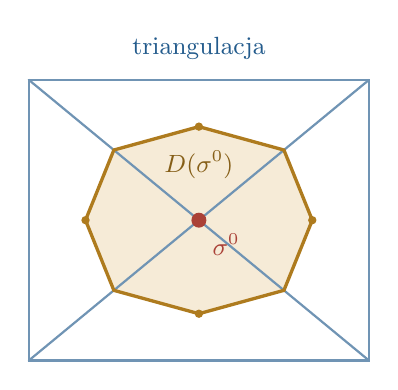
\begin{tikzpicture}[>=Latex,font=\small,line cap=round,scale=1.08]
 \coordinate (o) at (0,0);
 \coordinate (a) at (-2,-1.65);
 \coordinate (b) at (2,-1.65);
 \coordinate (c) at (2,1.65);
 \coordinate (d) at (-2,1.65);
 \fill[manifoldgold!18]
  (-1,-.825)--(0,-1.10)--(1,-.825)--
  ({4/3},0)--(1,.825)--(0,1.10)--
  (-1,.825)--({-4/3},0)--cycle;
 \draw[manifoldblue!65,thick] (a)--(b)--(c)--(d)--cycle;
 \foreach \v in {a,b,c,d}
  \draw[manifoldblue!65,thick] (o)--(\v);
 \draw[manifoldgold!85!black,very thick]
  (-1,-.825)--(0,-1.10)--(1,-.825)--
  ({4/3},0)--(1,.825)--(0,1.10)--
  (-1,.825)--({-4/3},0)--cycle;
 \foreach \x/\y in {0/-1.10,0/1.10}
  \fill[manifoldgold!85!black] (\x,\y) circle (1.4pt);
 \fill[manifoldgold!85!black] ({4/3},0) circle (1.4pt);
 \fill[manifoldgold!85!black] ({-4/3},0) circle (1.4pt);
 \fill[manifoldred] (o) circle (2.5pt)
  node[below right=2pt] {$\sigma^0$};
 \node[manifoldgold!65!black] at (0,.65) {$D(\sigma^0)$};
 \node[manifoldblue,anchor=south] at (0,1.78) {triangulacja};
\end{tikzpicture}
\caption{Niebieskie trójkąty stanowią fragment
triangulacji powierzchni. Złoty dysk jest
komórką dualną do środkowego wierzchołka.
Analogicznie krawędź ma dualną krawędź
przecinającą ją poprzecznie.}
\label{fig:dualna-komorka-16}
\end{figure}

\begin{twierdzenie}[Dualność Poincarégo]
\label{thm:poincare-dualnosc-16}
Dla zamkniętej zorientowanej
rozmaitości $M^n$ i dowolnych
abelowych grup współczynników $G$ mnożenie
kapowe przez klasę fundamentalną
jest izomorfizmem
\[
 \operatorname{PD}:H^k(M;G)
       \stackrel{\cong}{\longrightarrow}
       H_{n-k}(M;G),\qquad
 \alpha\longmapsto[M]\frown\alpha.
\]
Dla zwartej zorientowanej
rozmaitości z brzegiem
odpowiednie izomorfizmy to
\[
 H^k(M;G)\cong H_{n-k}(M,\partial M;G),
 \qquad
 H^k(M,\partial M;G)\cong H_{n-k}(M;G).
\]
Przy $G=\mathbb F_2$ orientacja
nie jest potrzebna.
\end{twierdzenie}
\begin{proof}
Najpierw niech $\partial M=\varnothing$.
Wybieramy dualny rozkład komórkowy
$K^\vee$. Ustalmy orientacje sympleksów. Dla $G=\Z$ niech
$\sigma^\#$ będzie kochainem równym $1$ na $\sigma$
i $0$ na pozostałych sympleksach tego wymiaru.
Orientujemy $D(\sigma)$ tak, aby kolejność
$(T\sigma,TD(\sigma))$ dawała orientację $M$.
Dla dowolnej grupy abelowej przenosimy po prostu
współczynnik $g\in G$ przy $\sigma^\#$ na tę komórkę.
Daje to izomorfizmy grup
\[
 \mathcal D_k:C^k(K;G)\longrightarrow C_{n-k}(K^\vee;G).
\]
Rachunek brzegu ma konkretny znak. Jeśli $\tau^{k+1}$
zawiera $\sigma^k$ i $u$ wskazuje od $\sigma$ do wnętrza
$\tau$, to konwencja brzegu daje
$\operatorname{or}(\tau)=[\tau:\sigma](-u,\operatorname{or}(\sigma))$.
Po przeniesieniu $u$ za $k$ wektorów otrzymujemy
$[\tau:\sigma](-1)^{k+1}(\operatorname{or}(\sigma),u)$.
W komórce dualnej kierunek $u$ wskazuje na zewnątrz
ku ścianie $D(\tau)$. Porównanie orientacji $M$ daje
\begin{equation}\label{eq:dualny-lancuch-16}
 \partial\mathcal D_k=(-1)^{k+1}\mathcal D_{k+1}\dd.
\end{equation}
Mimo znaku izomorfizmy $\mathcal D_k$ przenoszą
kocykle na cykle i kobrzegi na brzegi, zatem dają
$H^k(K;G)\cong H_{n-k}(K^\vee;G)$.
Jeśli chcemy dosłownego izomorfizmu kompleksów
z różniczkami $\dd$ i $\partial$, należy użyć
$(-1)^{k(k+1)/2}\mathcal D_k$. Zachowujemy jednak
nieprzeskalowane $\mathcal D_k$, zgodne ze znakiem
iloczynu kapowego w~\eqref{eq:kapowy-brzeg-16}.

Wyjaśnijmy utożsamienie z $[M]\frown\alpha$.
W podziale barycentrycznym obie konstrukcje dla
$\sigma^\#$ mają nośnik w zamkniętej gwieździe $\sigma$.
W stopniu $k=n$ dają punkty z tym samym współczynnikiem
orientacji. Różnicę można wypełnić drogą w tej gwieździe.
Schodząc kolejno z $k$ do $k-1$, z obu wzorów na brzeg
wynika, że różnica po odjęciu już zbudowanej homotopii
na kościanach jest cyklem w tej samej gwieździe.
Gwiazda jest ściągalna, więc cykl można wypełnić.
To indukcja analogiczna do dowodu przemienności
iloczynu kubkowego; daje homotopię po sprowadzeniu
obu konstrukcji do wspólnego podziału. Wyznaczają
więc to samo odwzorowanie na kohomologii, czyli $\operatorname{PD}$.
Oba rozkłady komórkowe obliczają homologię $M$.

Gdy $\partial M\ne\varnothing$,
dualna komórka przy brzegu
ma dodatkową ścianę
\emph{leżącą w brzegu}.
Po przejściu do łańcuchów
względnych ta ściana znika;
daje to pierwszy z podanych
izomorfizmów. Z kolei
kochainy względne znikają
na sympleksach brzegowych,
więc ich dualne komórki
nie mają obciętej ściany:
tworzą podkompleks dualny $L$ z komórek
$D(\sigma)$ dla $\sigma\not\subset\partial M$.
Ten podkompleks oblicza homologię $M$.
Istotnie, $M\setminus\partial M$ cofa się na $L$:
w każdym barycentrycznym sympleksie zerujemy wagi
wierzchołków odpowiadających ścianom brzegowym
i normalizujemy pozostałe. Ich suma jest dodatnia
poza brzegiem, a homotopia przez liniową zmianę wag
jest zgodna na ścianach. Włączenie wnętrza do $M$
jest równoważnością homotopijną, bo kołnierz pozwala
odsunąć brzeg do wnętrza. Stąd drugi izomorfizm
z homologii bezwzględnej.
W każdym przypadku
sprawdzenie~\eqref{eq:dualny-lancuch-16}
jest tym samym lokalnym
rachunkiem incydencji;
kołnierz z
Twierdzenia~\ref{thm:kolnierz-15}
zapewnia standardowy model
półprzestrzenny przy brzegu.
Nad $\mathbb F_2$ wszystkie
znaki orientacji znikają.
\end{proof}

\begin{wniosek}[Parowanie i charakterystyka Eulera]
\label{cor:pd-parowanie-16}
Dla zamkniętej zorientowanej
$M^n$ i ciała $\mathbb F$
parowanie
\[
 H^k(M;\mathbb F)\times
 H^{n-k}(M;\mathbb F)
 \longrightarrow\mathbb F,\qquad
 (\alpha,\beta)\longmapsto
      \langle\alpha\smile\beta,[M]\rangle
\]
jest niezdegenerowane. Zatem
$b_k=b_{n-k}$. Jeśli $n$
jest nieparzyste, $\chi(M)=0$.
\end{wniosek}
\begin{proof}
Dualność identyfikuje
$H^k$ z $H_{n-k}$.
Nad ciałem każda niezerowa
klasa homologii jest wykrywana
przez pewną klasę kohomologii
z $H^{n-k}$, bo dual przestrzeni
wektorowej rozdziela punkty.
Definicja iloczynu kapowego
i kubkowego utożsamia tę
ewaluację z podaną liczbą.
Stąd parowanie jest
niezdegenerowane i w skończonym
wymiarze obie strony mają
równe wymiary. Jeśli $n$
jest nieparzyste, w sumie
$\chi(M)=\sum_k(-1)^kb_k$
wyrazy dla $k$ i $n-k$
mają przeciwne znaki,
więc sumują się do zera.
\end{proof}

\begin{przyklad}[Torus i iloczyn dwóch sfer]
Na $T^2$ klasy
$a,b\in H^1(T^2;\Z)$,
odpowiadające dwóm kierunkom,
spełniają
$\langle a\smile b,[T^2]\rangle=1$
po ustaleniu orientacji.
Na $S^2\times S^2$ dwie
klasy $A,B\in H_2(-;\Z)$
reprezentowane przez
$S^2\times\{*\}$ i
$\{*\}\times S^2$
mają macierz przecięć
$\begin{psmallmatrix}0&1\\1&0\end{psmallmatrix}$.
Samych rang $H_2\cong\Z^2$
nie wystarcza do odtworzenia
tej macierzy.
\end{przyklad}

\section{Liczba przecięcia: znak i niezmienniczość}
\label{sec:przeciecia-16}

Niech $A^p,B^{n-p}\subset M^n$ będą
zamkniętymi zorientowanymi
podrozmaitościami zamkniętej
zorientowanej $M$. Po małej
perturbacji, możliwej dzięki
Twierdzeniu~\ref{thm:gestosc-transwersalnych},
możemy założyć $A\pitchfork B$.
Przecięcie ma wymiar zero,
a ze zwartości jest skończone.

\begin{definicja}[Znak i liczba przecięcia]
\index{znak i liczba przeciecia@Znak i liczba przecięcia}
\label{def:liczba-przeciecia-16}
Dla $x\in A\cap B$ kładziemy
$\epsilon_x=+1$, jeżeli
uporządkowana baza
$T_xA$ \emph{a następnie}
$T_xB$ daje orientację $T_xM$,
i $\epsilon_x=-1$ w przeciwnym
przypadku. \emph{Liczba
przecięcia} to
\[
 I(A,B)=\sum_{x\in A\cap B}\epsilon_x.
\]
Bez orientacji liczymy
$\#(A\cap B)\pmod 2$.
\end{definicja}

\begin{figure}[htbp]
\centering
\begin{tikzpicture}[>=Latex,font=\small,line cap=round,scale=1.04]
 \fill[manifoldblue!5] (-2.1,-1.65) rectangle (2.1,1.65);
 \draw[manifoldblue!45,thick]
   (-2.1,-1.65) rectangle (2.1,1.65);
 \draw[manifoldblue,very thick]
   (-2.1,0)--(2.1,0);
 \draw[manifoldblue,very thick,->]
   (1.25,0)--(1.75,0);
 \draw[manifoldgold!85!black,very thick]
   (0,-1.65)--(0,1.65);
 \draw[manifoldgold!85!black,very thick,->]
   (0,.60)--(0,1.10);
 \fill[manifoldred] (0,0) circle (2.6pt);
 \node[manifoldred,anchor=south west] at (.10,.08) {$x,\;\epsilon_x=+1$};
 \node[manifoldblue,anchor=north] at (1.35,-.12) {$A$};
 \node[manifoldgold!75!black,anchor=west] at (.12,1.15) {$B$};
 \node[anchor=south] at (0,1.72)
       {przeciwległe brzegi są sklejone};
\end{tikzpicture}
\caption{Dwa podstawowe okręgi torusa
przedstawionego jako kwadrat z parami
sklejonych boków. W punkcie $x$ kierunek
poziomy, po nim pionowy, daje dodatnią
orientację. Liczba przecięcia wynosi $1$.}
\label{fig:przeciecie-torus-16}
\end{figure}

\begin{twierdzenie}[Przecięcie i iloczyn kubkowy]
\label{thm:przeciecie-kubek-16}
Niech $\alpha_A=\operatorname{PD}^{-1}
(i_{A*}[A])\in H^{n-p}(M;\Z)$
i $\alpha_B=\operatorname{PD}^{-1}
(i_{B*}[B])\in H^p(M;\Z)$.
Przy konwencji orientowania przecięcia
z Definicji~\ref{def:liczba-przeciecia-16}
zachodzi
\begin{equation}\label{eq:przeciecie-kubek-16}
 I(A,B)=
 \langle\alpha_A\smile\alpha_B,[M]\rangle.
\end{equation}
Liczba zależy więc tylko od klas
homologii obu podrozmaitości;
jest niezmienna przy izotopii.
Jeżeli jest niezerowa, żadna
perturbacja w tych klasach nie
może rozdzielić $A$ i $B$.
\end{twierdzenie}
\begin{proof}
Użyjemy klasy Thoma z Twierdzenia~\ref{thm:euler-thom-16}.
Jej zamieszczony niżej dowód jest komórkowy i nie
korzysta z obecnego twierdzenia ani z klas $w_i$.
Orientujemy normalne warunkiem „normalna, potem styczna”.
Wycięcie w otoczeniu tubularnym daje klasy
$u_A\in H^{n-p}(M,M\setminus A;\Z)$ i
$u_B\in H^p(M,M\setminus B;\Z)$.
Ich obrazy w kohomologii bezwzględnej są $\alpha_A,\alpha_B$:
lokalnie oba opisy przypisują $+1$ dodatnio zorientowanemu
normalnemu dyskowi, co jest konstrukcją dualnej klasy.
Względny iloczyn ma nośnik na przecięciu, tzn.
\[
 u_A\smile u_B\in H^n(M,M\setminus(A\cap B);\Z).
\]
Wynika to z wersji względnej wzoru kubkowego:
po dostatecznym podziale sympleksy poza przecięciem
leżą w jednym z dwóch otwartych dopełnień,
gdzie odpowiedni czynnik znika.
Wycięcie rozkłada ostatnią grupę na sumę grup
$H^n(B_x,B_x\setminus\{x\};\Z)\cong\Z$
dla małych rozłącznych kul wokół punktów przecięcia.
Ewaluacja na $[M]$ jest sumą tych lokalnych liczb.
Jest to argument całkowity, nie tylko rachunek form
rzeczywistych, który mógłby zgubić torsję.

Oto kontrola znaku.
Niech $q=n-p$, a
$(a_1,\ldots,a_p)$
i $(b_1,\ldots,b_q)$
będą dodatnimi
bazami $T_xA$ i $T_xB$.
Załóżmy najpierw,
że $(a,b)$ orientuje
$T_xM$ dodatnio.
Normalną do $A$
orientujemy warunkiem
$(\nu_A,a)>0$,
a normalną do $B$
warunkiem
$(\nu_B,b)>0$.
Wówczas odpowiadająca
pierwszej normalnej
$q$-forma $\omega_A$
ma na bloku $b$
wartość $(-1)^{pq}$,
a $p$-forma $\omega_B$
drugiej normalnej
ma na bloku $a$
wartość $+1$.
We wzorze na
$(\omega_A\wedge\omega_B)(a,b)$
przestawienie bloku
$b$ przed $a$
daje drugi czynnik
$(-1)^{pq}$.
Iloczyn dwóch znaków
wynosi $+1$.
Odwrócenie orientacji
jednego z $A,B$
zmienia zarówno
$\epsilon_x$, jak
i tę wartość na $-1$.
Zatem lokalna ewaluacja
iloczynu jest $\epsilon_x$.
Po zsumowaniu po rozłącznych
małych otoczeniach punktów
przecięcia otrzymujemy
\eqref{eq:przeciecie-kubek-16}.
W powyższym rachunku formy $\omega_A,\omega_B$
opisują orientacje liniowych bloków; całkowite
generatory są ustalone przez klasy Thoma.
Poza tymi kulami nie ma wkładu dzięki względnemu
nośnikowi iloczynu. Ten sam dowód modulo $2$
działa bez orientacji. Dla transwersalnych przecięć
dodatniego wymiaru identyfikuje iloczyn klas Thoma
z klasą Thoma sumy normalnych; daje analogiczną
interpretację iloczynu jako klasy dualnej do przecięcia.

Prawa strona zależy jedynie
od $i_{A*}[A]$ i $i_{B*}[B]$,
ponieważ dualność Poincarégo
i iloczyn kubkowy są
określone na klasach.
Izotopijne zanurzenia
indukują homotopijne
odwzorowania w $M$,
więc dają tę samą
klasę homologii.
Gdyby obrazy dało się
rozłączyć, suma po
pustym przecięciu
wynosiłaby $0$.
\end{proof}

\begin{przyklad}[Krzywe na torusie]
W standardowej bazie
$H_1(T^2;\Z)=\Z a\oplus\Z b$
krzywe o klasach
$pa+qb$ i $ra+sb$
mają przecięcie algebraiczne
\[
 I\bigl((p,q),(r,s)\bigr)
 =\det\begin{pmatrix}p&r\\q&s\end{pmatrix}
 =ps-qr.
\]
Równość wynika z dwuliniowości
iloczynu i z
$I(a,b)=1$, $I(b,a)=-1$,
$I(a,a)=I(b,b)=0$.
Na przykład $(1,1)$ i $(1,-1)$
mają liczbę przecięcia $-2$:
co najmniej dwa przecięcia,
licząc bez znaków, są
nieuniknione w tych klasach.
Liczba $0$ nie gwarantuje
rozłączności konkretnych
przedstawicieli: dodatnie
i ujemne przecięcia mogą
się znosić.
\end{przyklad}

\begin{uwaga}[Samoprzecięcie]
Dwie kopie tej samej
podrozmaitości nie są
transwersalne, gdy się
pokrywają. Jedną z nich
przesuwamy w małym
otoczeniu tubularnym
za pomocą przekroju
wiązki normalnej.
Jeżeli przekrój ma zera,
przesunięta kopia
przecina pierwotną
właśnie w tych zerach.
Ta obserwacja prowadzi
do klasy Eulera
w Sekcji~\ref{sec:klasy-eulera-16}.
\end{uwaga}

\section{Lokalne współczynniki i brak orientacji}
\label{sec:lokalne-wsp-16}

Zwykła grupa współczynników
$\Z$ przyjmuje, że liczba
$+1$ oznacza to samo w
każdym punkcie. Na rozmaitości
nieorientowalnej lokalny
generator orientacji wraca
po pewnej pętli jako $-1$.
Trzeba więc przenosić
współczynniki wraz z drogą.

\begin{definicja}[System lokalny i system orientacji]
\index{system lokalny i system orientacji@System lokalny i system orientacji}
\label{def:system-lokalny-16}
\emph{System lokalny} grup abelowych
$\mathcal L$ przypisuje punktowi
$x$ grupę $\mathcal L_x$,
a drodze $\gamma:x\to y$
izomorfizm
$T_\gamma:\mathcal L_x\to\mathcal L_y$,
niezmienny przy homotopii
drogi z ustalonymi końcami
i zgodny ze składaniem dróg.
Transport wzdłuż drogi stałej jest identycznością.
Dla rozmaitości bez brzegu \emph{system orientacji}
$\mathcal O_M$ ma włókno
\[
 (\mathcal O_M)_x
  =H_n(M,M\setminus\{x\};\Z)
  \cong\Z;
\]
transport lokalnej orientacji
wzdłuż drogi jest mnożeniem
przez $+1$ albo $-1$. Przy brzegu definiujemy
system przez orientacje $T_xM$, równoważnie przez
przedłużenie systemu z wnętrza w kołnierzu.
Nie stosujemy tam powyższego wzoru na lokalną homologię.
\end{definicja}

W łańcuchach z $\mathcal L$
sympleks singularny ma
współczynnik w grupie
nad jego pierwszym
wierzchołkiem. Przy operatorze
brzegu współczynnik ściany
pomijającej pierwszy
wierzchołek przenosimy
wzdłuż pierwszej krawędzi
do nowego wierzchołka;
dla pozostałych ścian
punkt bazowy się nie
zmienia. Znaki przemienne
są takie jak w zwykłym
operatorze $\partial$.
Dwie drogi transportu
przy dwukrotnym usunięciu
wierzchołków są homotopijne
w obrębie sympleksu,
więc odpowiadające
wyrazy w $\partial^2$
znoszą się parami.
Tak powstaje
$H_*(M;\mathcal L)$.

\begin{przyklad}[Skręcone współczynniki na okręgu]
Niech $\mathcal L$ nad $S^1$
ma włókno $\Z$ i transport
po pełnym okrążeniu
równy $-1$. W komórkowym
modelu okręgu jest
jedna $0$-komórka
i jedna $1$-komórka.
Przy zwykłych
współczynnikach końce
krawędzi dają
$\partial_1=1-1=0$.
Tutaj jeden koniec
wraca ze znakiem
$-1$, więc
$\partial_1=(-1)-1=-2$.
Stąd
\[
 H_1(S^1;\mathcal L)=0,\qquad
 H_0(S^1;\mathcal L)=\Z/2.
\]
Po przejściu do
$\mathbb F_2$ macierz
$-2$ staje się zerem
i dostajemy zwykłe
grupy okręgu.
\end{przyklad}

\begin{twierdzenie}[Dualność ze skręconymi współczynnikami]
\label{thm:pd-skrecenie-16}
Dla spójnej zamkniętej
$n$-rozmaitości, także
nieorientowalnej, istnieje
kanoniczna skręcona klasa
fundamentalna
$[M]_{\mathcal O}\in
H_n(M;\mathcal O_M)$.
Dla stałej abelowej grupy
współczynników $G$
otrzymujemy izomorfizm
\[
 H^k(M;G)\cong
 H_{n-k}(M;\mathcal O_M\otimes G).
\]
Dla zwartej rozmaitości z brzegiem używamy
klasy $[M,\partial M]_{\mathcal O}$ i otrzymujemy
obie wersje względne:
\[
 H^k(M;G)\cong H_{n-k}(M,\partial M;\mathcal O_M\otimes G),
 \qquad
 H^k(M,\partial M;G)\cong H_{n-k}(M;\mathcal O_M\otimes G).
\]
Po zredukowaniu
współczynników modulo $2$
system orientacji staje
się stały.
\end{twierdzenie}
\begin{proof}
W każdej małej mapie
wybieramy generator
lokalnej homologii.
Gdy przechodzimy
do sąsiedniej mapy,
ewentualna zmiana
orientacji o $-1$
zmienia jednocześnie
współczynnik w
$\mathcal O_M$ o $-1$.
Iloczyn tych dwóch
znaków jest $+1$.
Suma wszystkich
najwyższych sympleksów
z tak dobranymi
lokalnymi współczynnikami
ma zatem zerowy brzeg
na każdej wspólnej
ścianie i daje
$[M]_{\mathcal O}$.
W małej kuli jej obraz
jest lokalnym generatorem.

W dowodzie
Twierdzenia~\ref{thm:poincare-dualnosc-16}
orientacja $M$ była
potrzebna do orientowania
komórek $D(\sigma)$.
Teraz orientujemy
$D(\sigma)$ za pomocą
lokalnego generatora
$(\mathcal O_M)_x$.
Przejście do sąsiedniej
komórki wnosi dokładnie
znak transportu
w $\mathcal O_M$.
Rachunek incydencji
\eqref{eq:dualny-lancuch-16}
pozostaje więc prawdziwy
z tymi współczynnikami.
Znowu dostajemy
izomorfizmy przenoszące jądra i obrazy
(ze znakiem zależnym od stopnia), a więc ich homologie.
Na brzegu przechodzimy
do łańcuchów względnych
tak samo jak w dowodzie
wersji zorientowanej.
W $\mathbb F_2$
mamy $-1=+1$,
więc monodromia znika.
\end{proof}

\begin{przyklad}[Wstęga Möbiusa i płaszczyzna rzutowa]
Dla wstęgi Möbiusa $W$
nie istnieje zwykła
całkowita klasa
$[W,\partial W]$
generująca orientację
we wszystkich punktach,
ale istnieje
$[W,\partial W]_{\mathcal O}
\in H_2(W,\partial W;\mathcal O_W)
\cong\Z$.
Dla $\R P^2$ mamy
$H_2(\R P^2;\Z)=0$,
za to
$H_2(\R P^2;\mathcal O)\cong\Z$
i $H_2(\R P^2;\mathbb F_2)
\cong\mathbb F_2$.
Lokalne współczynniki
odzyskują orientację
bez twierdzenia,
że przestrzeń nagle
stała się orientowalna.
\end{przyklad}

\section{Wiązki nad sferami i funkcje sklejające}
\label{sec:clutching-16}

Sferę $S^m$ rozkładamy na dwa
domknięte dyski $D^m_+$ i $D^m_-$,
sklejone wzdłuż równika
$S^{m-1}$. Wiązka wektorowa
nad każdym dyskiem jest
trywialna, ponieważ dysk
jest ściągalny. Cała informacja
o wiązce leży więc w
\emph{funkcji sklejającej}
na równiku.

\begin{twierdzenie}[Klasyfikacja przez równik]
\label{thm:clutching-16}
Dla $m\geq2$ klasy izomorfizmu zorientowanych
rzeczywistych wiązek
rzędu $r\geq1$ nad $S^m$
odpowiadają klasom homotopii
\[
 [S^{m-1},SO(r)]
 \cong\pi_{m-1}(SO(r)).
\]
Funkcja $g:S^{m-1}\to SO(r)$
skleja dwie wiązki
trywialne przez
$(x,v)_+\sim(x,g(x)v)_-$.
Izomorfizmy w tej klasyfikacji zachowują orientację włókien.
Dla niezorientowanych
wiązek nad $S^1$ pozostają
dwie klasy w każdym dodatnim
rzędzie: wiązka trywialna
i wiązka z jednym skręceniem
typu Möbiusa.
\end{twierdzenie}
\begin{proof}
Wybierzmy metrykę na włóknach
i dodatnio zorientowane ramy
nad $D^m_+$ i $D^m_-$.
Na ich wspólnym równiku
ramy różnią się macierzą
$g(x)\in SO(r)$. Otrzymujemy
opisane sklejenie, więc
każda wiązka jest takiej
postaci. Wybieramy ramy gładkie, na przykład przez transport
wzdłuż promieni dysków. Wtedy $g$ jest gładka;
klasy izomorfizmu
topologicznego i gładkiego
na sferze są tu zgodne
przez gładkie przybliżenie.

Zmiana ramy na górnym
lub dolnym dysku mnoży
$g$ z lewej lub prawej
przez ograniczenie
$h_\pm:D^m_\pm\to SO(r)$.
Każde takie ograniczenie
jest homotopijne do stałej:
ściągamy dysk do punktu.
Ponieważ $SO(r)$ jest
spójna dla $r\geq2$,
stałe macierze można
dalej połączyć z
jednostkową. Zatem
izomorfizm wiązek
nie zmienia klasy
homotopii $g$.
Dla $r=1$ grupa $SO(1)$
jest trywialna i wniosek
również jest prawdziwy.

Odwrotnie, gdy $g_t$ jest homotopią funkcji
sklejających, wygładzamy ją względnie końców i sklejamy
wiązki trywialne nad
$D^m_\pm\times[0,1]$
za pomocą $g_t$.
Powstaje wiązka nad
$S^m\times[0,1]$.
Wybierzmy na niej
metrykę i koneksję
(lokalne zwykłe pochodne
można skleić podziałem
jedności). Transport
równoległy w kierunku
od $t=0$ do $t=1$
zależy gładko od punktu
sfery i daje izomorfizm
wiązek na obu końcach.
To dowodzi, że homotopijne
funkcje sklejające
dają izomorficzne wiązki.
Stałość punktu bazowego
nie zmienia klasyfikacji dla spójnej grupy $SO(r)$.
Nie tylko odwzorowanie, ale i homotopię $g_t$ można
znormalizować: $\widetilde g_t(x)=g_t(x_0)^{-1}g_t(x)$
stale przyjmuje wartość $I$ w $x_0$. To pokazuje
injektywność i surjektywność przejścia od swobodnych
do opartych klas homotopii.

Nad $S^1$ równik to
dwa punkty $S^0$.
Po zmianie ramy w
jednym z dwóch łuków
pozostaje tylko informacja,
czy transport dookoła
okręgu ma wyznacznik
$+1$ czy $-1$.
Składowa $GL_r(\R)$
o wyznaczniku dodatnim
jest spójna, podobnie
ujemna; otrzymujemy
dokładnie dwie klasy.
\end{proof}

\begin{figure}[htbp]
\centering
\begin{tikzpicture}[>=Latex,font=\small,line cap=round,scale=1.08]
 \shade[inner color=white,outer color=manifoldblue!43]
    (0,0) circle (1.55);
 \fill[white,opacity=.38] (-1.55,0)
     arc[start angle=180,end angle=360,x radius=1.55,y radius=.41]
     --cycle;
 \draw[manifoldblue!75,very thick]
     (-1.55,0)
     arc[start angle=180,end angle=360,x radius=1.55,y radius=.41];
 \draw[manifoldblue!55,dashed]
     (-1.55,0)
     arc[start angle=180,end angle=0,x radius=1.55,y radius=.41];
 \node[manifoldblue!80!black] at (0,1.05) {$D^m_+$};
 \node[manifoldblue!80!black] at (0,-1.05) {$D^m_-$};
 \draw[->,manifoldgold!85!black,very thick]
   (2.20,.54) .. controls (2.85,.55) and (2.85,-.55) .. (2.20,-.54);
 \node[anchor=west,manifoldgold!75!black] at (2.8,.03)
     {$g:S^{m-1}\to SO(r)$};
 \node[anchor=west] at (-1.30,-1.88)
     {dwie trywializacje spotykają się na równiku};
\end{tikzpicture}
\caption{Sfera jako dwa dyski z równikiem.
W każdej połowie wiązka jest iloczynem;
macierz $g(x)$ mówi, jak zidentyfikować
włókna po obu stronach równika.}
\label{fig:clutching-16}
\end{figure}

\begin{przyklad}[Dlaczego $TS^2$ jest skręcona]
Zorientowane wiązki płaszczyznowe
nad $S^2$ opisuje
$\pi_1(SO(2))=\pi_1(S^1)=\Z$.
Dla wiązki $TS^2$ wybierzmy
stereograficzne zespolone
współrzędne $z$ i $w$
na półkulach z przejściem
$w=1/z$ w pasie równika.
Pochodna przejścia
$\dd w/\dd z=-z^{-2}$
obraca ramę styczną
dwukrotnie, gdy $z$
okrąża równik raz.
Funkcja sklejająca ma
więc liczbę nawinięć
$\pm2$ (znak zależy
od wyboru orientacji
równika). Wiązka $TS^2$
nie jest trywialna:
na sferze nie istnieje
globalna rama dwóch
niezależnych pól stycznych.
\end{przyklad}

\begin{przyklad}[Grupa obrotów w wymiarze trzy]
Dla zorientowanych wiązek
rzędu $3$ nad $S^2$
otrzymujemy
$\pi_1(SO(3))\cong\Z/2$:
są dwie klasy.
Opis podwójnego nakrycia
$\operatorname{Spin}(3)\to SO(3)$
z Rozdziału~\ref{ch:grass-spin}
pokazuje, skąd bierze się
dwójka. Pętla macierzy
obrotu reprezentująca
klasę niezerową podnosi
się do drogi kończącej
w drugim punkcie włókna
nakrycia. Takiej
funkcji sklejającej
nie można podnieść
do zamkniętej pętli
w $\operatorname{Spin}(3)$;
wiązka ma niezerowe
$w_2\in H^2(S^2;\mathbb F_2)$.
Wiązka trywialna ma
$w_2=0$.
\end{przyklad}

\section{Klasy charakterystyczne: przeszkody w kohomologii}
\label{sec:klasy-char-16}

\begin{definicja}[Idea klasy charakterystycznej]
\index{idea klasy charakterystycznej@Idea klasy charakterystycznej}
Klasą charakterystyczną
wiązki $E\to M$ nazywamy
przypisanie $E\mapsto c(E)
\in H^k(M;G)$ zgodne
z cofnięciem:
$c(f^*E)=f^*c(E)$.
Jeżeli wiązka jest trywialna,
jej klasy dodatniego stopnia
są zerowe, bo jest cofnięciem
wiązki nad punktem.
Odwrotna implikacja
nie musi zachodzić:
klasy charakterystyczne
nie rozróżniają wszystkich
wiązek.
\end{definicja}

Najbardziej elementarna
przeszkoda dotyczy
orientacji. Nie trzeba
jej definiować przez
ogólną teorię przestrzeni
klasyfikujących.

\begin{stwierdzenie}[Pierwsza klasa Stiefela--Whitneya]
\label{prop:w1-orientacja-16}
Niech $E\to M$ będzie
rzeczywistą wiązką
rzędu $r$. Wybierzmy
trywializacje nad dobrym
pokryciem $\{U_i\}$ i
funkcje przejścia
$g_{ij}:U_i\cap U_j\to GL_r(\R)$.
Znaki
$\epsilon_{ij}=\operatorname{sgn}
\det g_{ij}\in\{\pm1\}$
wyznaczają klasę
$w_1(E)\in H^1(M;\mathbb F_2)$.
Mamy $w_1(E)=0$
wtedy i tylko wtedy,
gdy $E$ jest orientowalna.
Ponadto
$w_1(E\oplus F)=w_1(E)+w_1(F)$.
\end{stwierdzenie}
\begin{proof}
Na potrójnym przecięciu
$g_{ij}g_{jk}=g_{ik}$,
a więc
$\epsilon_{ij}\epsilon_{jk}
=\epsilon_{ik}$.
Po utożsamieniu $-1$
z $1\in\mathbb F_2$
jest to równanie jednokocyklu. Aby utożsamić jego
klasę z kohomologią singularną, można obyć się
bez dodatkowego formalizmu: mnożymy znaki przejść
wzdłuż pętli. Warunek na potrójnych przecięciach
zapewnia niezmienniczość przy podziale i homotopii
pętli, a więc homomorfizm $\pi_1(M)\to\mathbb F_2$.
Utożsamienia $H_1(M;\Z)=\pi_1(M)_{\mathrm{ab}}$
i $H^1(M;\mathbb F_2)=\operatorname{Hom}(H_1(M;\Z),\mathbb F_2)$
dają żądaną klasę na każdej składowej. Gdy homomorfizm
znika, transport orientacji z ustalonego punktu nie
zależy od drogi i nadaje zgodne orientacje lokalnym ramom.
Zmiana
ramy na $U_i$ mnoży
każdy znak $\epsilon_{ij}$
przez znak nowej ramy
na $U_i$ i na $U_j$;
odpowiada to dodaniu
kobrzegu, więc klasa
nie zależy od ram.
Jeśli $w_1(E)=0$,
kocykl znaków jest
kobrzegiem: zmieniamy
orientacje lokalnych
ram tak, aby wszystkie
macierze przejścia
miały dodatni wyznacznik.
Ramy nadają wtedy
spójną orientację
wiązce. Odwrotnie
spójna orientacja
pozwala od początku
wybrać takie ramy
i daje kocykel zerowy.
Macierz przejścia
dla $E\oplus F$
jest blokowa,
$\det(g_{ij}\oplus h_{ij})
=\det(g_{ij})\det(h_{ij})$;
znaki mnożą się, a
w $\mathbb F_2$
ich klasy się dodają.
\end{proof}

\begin{przyklad}
Wiązka Möbiusa nad $S^1$
ma monodromię $-1$,
więc $w_1$ jest
niezerowym elementem
$H^1(S^1;\mathbb F_2)$.
Trywialna linia ma $w_1=0$.
Dla rozmaitości
$w_1(TM)$ jest dokładnie
przeszkodą do jej
orientowalności.
Jest to również
monodromia systemu
$\mathcal O_M$
z Sekcji~\ref{sec:lokalne-wsp-16}.
\end{przyklad}

\begin{twierdzenie}[Pełna rodzina $w_i$]
\label{thm:wi-klasy-16}
Dla wiązki rzeczywistej
$E$ rzędu $r$ istnieją
klasy Stiefela--Whitneya
\[
 w_i(E)\in H^i(M;\mathbb F_2),
 \quad 0\leq i\leq r,\qquad
 w_0=1,\quad w_i=0\ (i>r),
\]
naturalne przy cofnięciu.
Dla sumy wiązek
\[
 w(E\oplus F)=w(E)\smile w(F),
 \qquad w(E)=1+w_1(E)+\cdots+w_r(E).
\]
W szczególności dla zanurzenia
$S\subset M$ z
Rozdziału~\ref{ch:wlozenia-otoczenia}
zachodzi
\begin{equation}\label{eq:w-normalne-16}
 w(TM|_S)=w(TS)\smile w(\nu(S,M)).
\end{equation}
\end{twierdzenie}
\begin{proof}
Dla $r=0$ przyjmujemy $w(E)=1$; dalej $r\geq1$.
Korzystamy z niezależnej konstrukcji klasy Thoma
i klasy $e_2$ poniżej. Dowód tej konstrukcji nie
zakłada istnienia $w_i$; zależności wyjaśnia uwaga
po Twierdzeniu~\ref{thm:euler-thom-16}.

Uzasadnijmy najpierw potrzebny rachunek we włóknie.
Na $\R P^m$ niech $x=w_1(\lambda)$ dla linii
tautologicznej. Ograniczenie ustalonego funkcjonału
liniowego do $\lambda$ jest przekrojem $\lambda^*$,
którego zera tworzą hiperpłaszczyznę $\R P^{m-1}$.
Parzystość przecięć pętli z tą hiperpłaszczyzną
jest zmianą znaku jej podniesienia do jednostkowych
wektorów linii: funkcjonał zmienia znak przy każdym
poprzecznym przejściu przez zero. Jest to dokładnie
monodromia $w_1$, więc hiperpłaszczyzna jest dualna do $x$.
$j$ niezależnych hiperpłaszczyzn przecina się
transwersalnie, a w $\R P^j$ ich przecięcie jest
jednym punktem. Modułowa wersja rachunku przecięć daje
$\langle x^j,[\R P^j]_2\rangle=1$.
Z obliczenia komórkowego grup $\R P^m$ wiemy, że
każda grupa $H^j(-;\mathbb F_2)$ dla $0\leq j\leq m$
jest jednowymiarowa. Zatem $1,x,\ldots,x^m$ są bazą,
a $x^{m+1}=0$ z przyczyn wymiarowych.

Podajemy konstrukcję algebraiczną klas ogólnej wiązki.
Niech $\pi:P(E)\to M$ będzie wiązką
prostych we włóknach $E$,
$\lambda\to P(E)$ wiązką
tautologiczną, a
$x=w_1(\lambda)\in
H^1(P(E);\mathbb F_2)$.
Włóknem $P(E)$ jest
$\R P^{r-1}$; klasy
$1,x,\ldots,x^{r-1}$
po ograniczeniu do
każdego włókna tworzą
bazę jego kohomologii.
Stąd
\[
 H^*(P(E);\mathbb F_2)
  =\bigoplus_{j=0}^{r-1}
     H^*(M;\mathbb F_2)\,x^j
\]
jako moduł nad $H^*(M)$.
Rozpiszmy ten szczególny przypadek twierdzenia Leraya--Hirscha.
Wybieramy triangulację $M$ i oznaczamy przez $M^{(d)}$ jej
$d$-szkielet, z $M^{(-1)}=\varnothing$. Dla pary podkompleksów
$A\subset B$ i $P_B=\pi^{-1}(B)$, $P_A=\pi^{-1}(A)$ definiujemy
łączne odwzorowanie
\[
 \Phi^q_{B,A}:\bigoplus_{j=0}^{r-1}H^{q-j}(B,A;\mathbb F_2)
 \longrightarrow H^q(P_B,P_A;\mathbb F_2),
 \qquad (a_j)_j\longmapsto\sum_{j=0}^{r-1}\pi^*a_j\smile x^j.
\]
Klasy $x^j$ po prawej ograniczamy do $P_B$; używamy iloczynu
klasy względnej z klasą bezwzględną. Grupy w stopniach ujemnych są zerowe.
Izomorfizmem ma być cała suma $\Phi^q_{B,A}$, nie każdy jej składnik.

Dla $B=M^{(d)}$ i $A=M^{(d-1)}$ wycinanie rozdziela rachunek względny
na dołączane $d$-komórki. Nad dyskiem charakterystycznym każdej
z nich cofnięta wiązka jest trywialna, więc otrzymujemy parę
\[
 (D^d\times\R P^{r-1},\ \partial D^d\times\R P^{r-1}).
\]
Jej kohomologia w stopniu $q$ to $H^{q-d}(\R P^{r-1};\mathbb F_2)$:
w względnym kompleksie komórkowym jedyna komórka dysku modulo
brzeg przesuwa stopnie kompleksu włókna o $d$.
Iloczyn generatora $H^d(D^d,\partial D^d;\mathbb F_2)$ z $x^j$
odpowiada elementowi $x^j$ tej grupy w stopniu $q=d+j$.
Sprawdzona baza $1,x,\ldots,x^{r-1}$ dowodzi zatem, że
$\Phi^q_{M^{(d)},M^{(d-1)}}$ jest izomorfizmem.
Przy nieskończenie wielu komórkach grupy kochainów są produktami;
suma po $j$ ma jednak tylko $r$ składników, więc komutuje z tymi
produktami i ten sam wniosek pozostaje prawdziwy.

Dla kolejnych szkieletów i ich przeciwobrazów odwzorowania $\Phi$
tworzą przemienny diagram długich ciągów dokładnych par.
Zgodność z ograniczeniami wynika z naturalności iloczynu kubkowego,
a z homomorfizmami łączącymi --- z reguły Leibniza dla zamkniętych
reprezentantów $x^j$. Nad $\mathbb F_2$ nie występuje dodatkowy znak.
Zaczynając od pustego szkieletu, stosujemy lemat o pięciu
odwzorowaniach: izomorfizm na poprzednim szkielecie i izomorfizm
względny dają izomorfizm na następnym szkielecie.
Triangulacja ma wymiar $\dim M$, więc także dla niezwartych $M$
indukcja kończy się po skończenie wielu stopniach. Dla $A=\varnothing$
otrzymujemy zapowiedziany rozkład modułu. Ogólną wersję tego argumentu
podaje Hatcher, \emph{Algebraic Topology}, Twierdzenie~4D.1.

Klasa $x^r$ ma wobec
tej bazy jednoznaczny
rozkład. Zapisujemy
go w postaci
\[
 x^r+
   \pi^*w_1(E)x^{r-1}
     +\cdots+\pi^*w_r(E)=0.
\]
Współczynnik $w_i$
ma stopień $i$,
bo każdy wyraz ma
całkowity stopień $r$.
Jednoznaczność rozkładu
i zgodność konstrukcji
$P(E)$ z cofnięciem
dają naturalność.
Przy rozszczepieniu
$E=L_1\oplus\cdots\oplus L_r$
relacja włóknowa
ma czynniki
$\prod_j(x+w_1(L_j))$.
Oto bezpośrednie
sprawdzenie. Nad $P(E)$
tautologiczna linia
$\lambda$ wchodzi
do $\pi^*E$, więc
homomorfizm inkluzji
jest nigdzie
nieznikającym
przekrojem wiązki
$\operatorname{Hom}(\lambda,\pi^*E)
=\bigoplus_j(\lambda^*\otimes\pi^*L_j)$.
Jej klasa Eulera modulo $2$, oznaczana niezależnie
przez $e_2$, jest zatem zerowa
na mocy
Twierdzenia~\ref{thm:euler-thom-16}
i uwagi o redukcji
modulo $2$ w
Sekcji~\ref{sec:klasy-eulera-16}.
Klasa Eulera modulo $2$
linii jest jej
$w_1$, a
$w_1(\lambda^*\otimes L_j)
=x+w_1(L_j)$
z rachunku znaków
funkcji przejścia.
Multiplikatywność
klasy Eulera sumy
daje właśnie
$\prod_j(x+w_1(L_j))=0$.
Porównanie współczynników
daje
$w(E)=\prod_j(1+w_1(L_j))$.

Każdą wiązkę można
rozszczepić po cofnięciu
do wiązki pełnych flag:
po kolei wybieramy
prostą w $E$ i w
ortogonalnym do niej
dopełnieniu. W każdym
takim kroku powyższy
rozkład modułowy
zawiera składnik $1$,
więc cofnięcie
na kohomologiach
jest injektywne.
Wzór iloczynowy
sprawdzony po
rozszczepieniu
schodzi zatem na $M$
i daje twierdzenie o sumie Whitneya. Dla dwóch
wiązek najpierw rozszczepiamy $E$, potem cofniętą $F$;
oba cofnięcia są injektywne, a obie wiązki rozszczepione.
Współczynnik stopnia jeden jest $\sum_jw_1(L_j)$,
czyli wcześniej zdefiniowany znak wyznacznika przejść.
Nowa definicja $w_1$ jest więc zgodna z poprzednią.
Wreszcie
$TM|_S\cong TS\oplus\nu$
z
Stwierdzenia~\ref{prop:normalna-rozszczepienie};
podstawienie do wzoru
sumy daje~\eqref{eq:w-normalne-16}.
\end{proof}

\begin{uwaga}[Gdzie już pojawiło się $w_2$?]
W Rozdziale~\ref{ch:grass-spin}
skonstruowaliśmy
$w_2(E)$ dla zorientowanej
wiązki jako przeszkodę
podniesienia funkcji
przejścia z $SO(r)$
do $\operatorname{Spin}(r)$.
Wyjaśnijmy zgodność z klasą stopnia dwa z
Twierdzenia~\ref{thm:wi-klasy-16}. Wystarczy ograniczyć
się do $2$-szkieletu bazy: restrykcja $H^2(M;\mathbb F_2)$
do tego szkieletu jest injektywna, ponieważ grupy
kochainów i kobrzegi w stopniach $1,2$ są te same.
Na kompleksie wymiaru dwa wiązka rzędu co najmniej trzy
ma niezerowy przekrój: wybieramy go na wierzchołkach,
przedłużamy po krawędziach przez spójność sfery włókna,
a po $2$-komórkach przez jej jednospójność.
Powtarzając, rozszczepiamy zorientowaną wiązkę na
trywialną część i zorientowaną płaszczyznę $L$.
Wzór sumy daje $w_2(E)=w_2(L)=e(L)\bmod2$.
Wybierzmy zorientowaną ramę $L$ na $1$-szkielecie;
jest to możliwe dzięki spójności $SO(2)$.
Na $2$-komórce, względem tej ustalonej ramy brzegowej,
ostatnia liczba jest parzystością liczby nawinięć
funkcji $SO(2)$, bo to
stopień przeszkody przedłużenia niezerowego przekroju.
Ta sama parzystość jest przeszkodą podniesienia pętli
do $\operatorname{Spin}(2)\to SO(2)$, nakrycia $z\mapsto z^2$.
Po dodaniu kierunków trywialnych obrót o $2\pi$
nadal podnosi się do drogi od $1$ do $-1$ w grupie Spin.
Oba kocykle na $2$-komórkach są więc równe,
co dowodzi zgodności klas. Dla rzędu jeden obie są zerowe.
Z warunku
\eqref{eq:w-normalne-16}
wynika, że jeśli
$\nu(S,M)$ ma obramowanie,
to $w(\nu)=1$ i
$w(TM)|_S=w(TS)$.
To prosty test konieczny
dla niektórych zanurzeń
obramowanych.
\end{uwaga}

\begin{uwaga}[Klasy zespolone i Pontriagina]
Dla zespolonej wiązki
rzędu $r$ analogiczna
konstrukcja z
$\C P^{r-1}$
i klasą pierwszą
tautologicznej linii
o stopniu $2$
daje klasy Cherna
$c_i(E)\in H^{2i}(M;\Z)$.
Dla wiązki rzeczywistej
klasy Pontriagina
definiuje się przez
$p_i(E)=(-1)^i
c_{2i}(E\otimes_\R\C)
\in H^{4i}(M;\Z)$.
Ich naturalność i
zgodność ze stabilnym
dołożeniem wiązki
trywialnej wynikają
z konstrukcji projektowej.
W tym rozdziale
szczegółowo stosujemy
$w_1,w_2$ i klasę
Eulera; pełny rachunek
klas $c_i,p_i$
oraz konstrukcja
Cherna--Weila
wykraczają poza
niezbędne przygotowanie
do chirurgii.
\end{uwaga}

\section{Klasa Eulera, zera pól i samoprzecięcie}
\label{sec:klasy-eulera-16}

\begin{twierdzenie}[Klasa Thoma i klasa Eulera]
\label{thm:euler-thom-16}
Niech $E\to M$ będzie
zorientowaną rzeczywistą
wiązką rzędu $r$ z metryką
we włóknach. Dla jej
wiązki dysków $D(E)$
i wiązki sfer $S(E)$
istnieje klasa
\[
 u_E\in H^r(D(E),S(E);\Z),
\]
której ograniczenie do
każdego włókna
$(D^r,S^{r-1})$ jest
dodatnim generatorem.
Iloczyn z $u_E$ daje
izomorfizm Thoma
\[
 H^j(M;\Z)\stackrel{\cong}{\longrightarrow}
 H^{j+r}(D(E),S(E);\Z).
\]
Jeśli $s_0:M\to D(E)$
jest przekrojem zerowym,
to \emph{klasa Eulera}
$e(E)=s_0^*u_E\in H^r(M;\Z)$
jest naturalna przy
cofnięciu i spełnia
$e(E\oplus F)=e(E)\smile e(F)$
dla zorientowanych wiązek.
Istnienie nigdzie nieznikającego
przekroju pociąga $e(E)=0$.
\end{twierdzenie}

W zapisie $s_0^*u_E$ najpierw zapominamy o względności,
przechodząc z $H^r(D(E),S(E))$ do $H^r(D(E))$,
a potem cofamy klasę przez $s_0$. Równoważnym modelem
klasy Thoma jest $H^r(E,E\setminus0)$: wycięcie
i radialne cofnięcie włókien utożsamiają go z modelem
dyskowym. Ten model pozwala cofać klasę przez przekrój
jako klasę pary $(M,M\setminus Z(s))$.

\begin{proof}
Nad komórką bazy wiązka jest trywialna, zatem odpowiednia
para w przestrzeni całkowitej jest iloczynem tej komórki
z parą $(D^r,S^{r-1})$.
Włóknowa grupa względna
w stopniu $r$ jest $\Z$;
orientacja określa jej
dodatni generator.
Na przecięciu sąsiednich
trywializacji macierz
przejścia ma dodatni
wyznacznik, więc przenosi
ten generator w niego
samego. Sama zgodność lokalnych generatorów nie jest jeszcze
dowodem istnienia globalnej klasy. Skonstruujmy ją
w kompleksie komórkowym pary $(D(E),S(E))$.
Nad każdą $d$-komórką bazy dołączamy względną
komórkę $D^d\times D^r$ wymiaru $d+r$;
część $D^d\times S^{r-1}$ leży już w $S(E)$,
a $\partial D^d\times D^r$ nad wcześniejszym szkieletem.
Orientujemy iloczyn kolejnością „baza, włókno”.
Liczby incydencji są tymi z bazy pomnożonymi
przez stopień transportu orientacji włókna, czyli $+1$.
Kompleks względny kochainów jest więc kompleksem
bazy przesuniętym o $r$. Stały kocykl $1$ w stopniu
zero bazy wyznacza kocykl stopnia $r$ pary,
którego klasa to $u_E$. Jest to jedyna klasa
o wymaganych ograniczeniach: pod tym przesunięciem
odpowiada funkcji na składowych bazy o wartości $1$.
Dla niezwartej bazy używamy produktów współczynników
po komórkach; indukcja po szkieletach ma skończenie
wiele etapów, gdyż rozmaitość ma skończony wymiar.

Teraz sprawdzamy, że mnożenie przez tę już
skonstruowaną klasę daje deklarowany izomorfizm:
na dołączanej $d$-komórce
relatywne grupy pary
wiązki są przesunięciem
o $r$ relatywnych grup
$(D^d,S^{d-1})$.
Mnożenie przez lokalny
generator jest tam
izomorfizmem. W długich
ciągach dokładnych
dla starego szkieletu
i nowej komórki wszystkie
kwadraty są naturalne;
indukcja i lemat o
pięciu odwzorowaniach
dają izomorfizm w
każdym stopniu.
Mnożenie ma dokładnie postać
$a\mapsto\pi^*a\smile u_E$; na każdej komórce
jest opisanym przesunięciem przez włóknowy generator.
Dla rzędu zero przyjmujemy $S(E)=\varnothing$
i $u_E=e(E)=1$.

Cofnięcie wiązki przenosi
orientacje i włóknowe
generatory, więc przenosi
$u_E$ na klasę Thoma
cofniętej wiązki. Po
ograniczeniu do
przekroju zerowego
daje to naturalność
$e(f^*E)=f^*e(E)$.
Dla sumy $E\oplus F$ możemy użyć dysku w normie
maksimum, czyli $D(E)\times_M D(F)$. Jego brzeg to
$(S(E)\times_M D(F))\cup(D(E)\times_M S(F))$.
Cofamy obie klasy Thoma przez rzuty i bierzemy
ich względny iloczyn kubkowy. W każdym włóknie
jest on dodatnim generatorem w orientacji „$E$, potem $F$”,
więc z jedyności jest klasą Thoma sumy.
Zmiana normy przez radialny homeomorfizm nie zmienia
klasy. Cofnięcie do zera daje
$e(E\oplus F)=e(E)\smile e(F)$.

Jeśli $s$ nigdzie
nie znika, po unormowaniu
jest odwzorowaniem
$M\to S(E)$.
Włączenie $S(E)\subset D(E)$
powoduje $s^*u_E=0$,
bo względna klasa
na $S(E)$ znika.
Przekroje $s_0$ i $s$
są homotopijne jako
odwzorowania $M\to D(E)$
przez $t\mapsto ts$.
Ich cofnięcia klasy
$u_E$ są więc równe;
$e(E)=0$.
\end{proof}

\begin{uwaga}[Wersja modulo $2$ i brak błędnego koła]
Powyższy dowód nie używa klas Stiefela--Whitneya.
Z $\mathbb F_2$ działa dla każdej wiązki, ponieważ
zmiana orientacji włókna nie zmienia generatora.
Oznaczmy otrzymaną klasę Eulera modulo $2$ przez $e_2(E)$.
Jest naturalna, multiplikatywna i znika przy istnieniu
niezerowego przekroju, z dokładnie tych samych dowodów.

Dla linii $L$ mamy $e_2(L)=w_1(L)$. Wybierzmy
niezerowe wartości przekroju w wierzchołkach triangulacji
i przedłużmy go ogólnie na krawędzie. Parzystość zer
na krawędzi wynosi $1$ dokładnie wtedy, gdy wartości
na końcach mają przeciwne znaki po transporcie
w trywializacji tej krawędzi. Jest to kocykl zmiany
orientacji, czyli $w_1(L)$; zmiana wartości przy
wierzchołku dodaje kobrzeg. Z drugiej strony te same
parzystości są lokalnymi stopniami cofnięcia klasy Thoma,
więc reprezentują $e_2(L)$.

Te własności $e_2$ wystarczają do dowodu wzoru
w Twierdzeniu~\ref{thm:wi-klasy-16}; nie zakłada on
z góry równości $e_2=w_r$. Dopiero po rozszczepieniu
$E$ na linie otrzymujemy
$e_2(E)=\prod_jw_1(L_j)=w_r(E)$.
Injektywność cofnięcia do wiązki flag przenosi
tę równość na bazę. Dla wiązki zorientowanej
redukcja całkowitej klasy Thoma jest klasą Thoma modulo $2$,
więc również $e(E)\bmod2=w_r(E)$.
\end{uwaga}

\begin{twierdzenie}[Zera przekroju reprezentują klasę Eulera]
\label{thm:euler-zeros-16}
Niech $M^n$ będzie
zamknięta i zorientowana,
a $E\to M$ zorientowana
rzędu $r\leq n$.
Dla przekroju $s$
transwersalnego do zera
zbiór $Z(s)$ jest
zorientowaną
$(n-r)$-podrozmaitością i
\[
 \operatorname{PD}^{-1}[Z(s)]=e(E).
\]
Jeśli $r=n$, zera są
skończone i
\begin{equation}\label{eq:euler-zeros-16}
 \langle e(E),[M]\rangle
   =\sum_{x\in Z(s)}
       \operatorname{sgn}\det(\D_xs).
\end{equation}
W bazach zgodnych z
orientacją znak nie
zależy od wyboru
trywializacji.
\end{twierdzenie}
\begin{proof}
Regularność wynika z Twierdzenia~\ref{thm:zera-przekroju}.
Pochodna pionowa w zerze daje izomorfizm
$\nu(Z(s),M)\cong E|_{Z(s)}$. Nadajemy normalnej
orientację przeniesioną z $E$, a $Z(s)$ orientujemy
warunkiem „normalna, potem styczna daje orientację $M$”.

W modelu $H^r(E,E\setminus0)$ cofnięcie przez $s$
jest klasą $s^*u_E\in H^r(M,M\setminus Z(s))$.
W małej trywializacji ograniczenie $s$ do normalnego
dysku ma w zerze odwracalną różniczkę o dodatnim
wyznaczniku, więc jego lokalny stopień jest $+1$.
Wycięcie i otoczenie tubularne identyfikują
$s^*u_E$ z klasą Thoma normalnej do $Z(s)$.
Jej obraz w kohomologii bezwzględnej jest klasą
dualną do $Z(s)$: na każdej normalnej komórce
ocenia $+1$, zgodnie z orientacjami w dowodzie dualności.
Liniowa homotopia $s\simeq s_0$ w $E$ pokazuje,
że ten sam obraz jest $e(E)$.

Dla $r=n$ każdy punkt zerowy jest zorientowaną
$0$-komórką o współczynniku
$\operatorname{sgn}\det\D_xs$. Zwartość i izolacja
zer dają ich skończoność. Ewaluacja na klasie
fundamentalnej sumuje te współczynniki,
co daje~\eqref{eq:euler-zeros-16}.
\end{proof}

\begin{wniosek}[Samoprzecięcie]
\label{cor:samoprzeciecie-16}
Niech $M^{2k}$ będzie zorientowana, a
$S^k\subset M$ zamknięta i zorientowana.
W tym wzorze nadajemy wiązce normalnej orientację
przez kolejność \emph{styczna do $S$, potem normalna},
zgodną z orientacją $M$. Wówczas
to liczba przecięcia
$S$ z małą przesuniętą
kopią wynosi
\[
 I(S,S)=\langle e(\nu(S,M)),[S]\rangle.
\]
\end{wniosek}
\begin{proof}
W otoczeniu tubularnym
zapisujemy $S$ jako
przekrój zerowy $\nu$.
Wybierzmy mały przekrój
$s$ transwersalny do
zera i przesuńmy $S$
do jego wykresu.
Wykres przecina
przekrój zerowy
dokładnie dla $s(x)=0$.
W bazach „styczna, normalna” kolumny baz
przekroju zerowego i wykresu tworzą macierz
$\begin{psmallmatrix}I&I\\0&\D_xs\end{psmallmatrix}$.
Jej wyznacznik to $\det\D_xs$, więc znak przecięcia
jest lokalnym stopniem $s$. Ten rachunek ustala
potrzebną orientację normalnej; nie można jej
odwrócić dowolnie, zachowując ten sam zapis wzoru.
Suma znaków to
$\langle e(\nu),[S]\rangle$
z~\eqref{eq:euler-zeros-16}.
\end{proof}

\begin{przyklad}
Dla $S^2\times\{p\}
\subset S^2\times S^2$
wiązka normalna jest
trywialna: jej włókno
to stała przestrzeń
$T_pS^2$. Istnieje
niezerowy stały
przekrój, więc
$I(S,S)=0$.
Dwie różne sfery
$S^2\times\{p\}$
i $\{q\}\times S^2$
przecinają się
jednak w jednym
punkcie z liczbą
przecięcia $1$.
\end{przyklad}

\section{Twierdzenie Poincarégo--Hopfa}
\label{sec:poincare-hopf-16}

\begin{definicja}[Indeks zera pola]
\index{indeks zera pola@Indeks zera pola}
Jeżeli pole $X$ na
$n$-rozmaitości ma
izolowane zero $x$,
wybierzmy małą kulę w mapie wokół $x$
oraz trywializację stycznej przez różniczkę tej mapy.
\emph{Indeks} $\operatorname{ind}_x X$
jest stopniem odwzorowania
$X/|X|:S^{n-1}\to S^{n-1}$, dla $n\geq1$.
Zmiana mapy zmienia jednocześnie orientację dziedziny
i współrzędnych wektora, więc dwa znaki się mnożą
do $+1$. Zmienną macierz przejścia na małej kuli
można zdeformować do jej wartości w środku, nie
przechodząc przez macierze osobliwe. Indeks nie
zależy więc od mapy ani od lokalnej orientacji.
Dla $n=1$ stopień liczymy na $\widetilde H_0(S^0)$;
dla $n=0$ umownie każdy punkt zerowy ma indeks $1$.
Jeśli $\D_xX$ jest
odwracalna,
$\operatorname{ind}_xX
=\operatorname{sgn}\det\D_xX$:
na małej sferze
$X(y)=\D_xX(y-x)+o(|y-x|)$
jest homotopijne
do odwracalnej
odwzorowania liniowego.
\end{definicja}

\begin{twierdzenie}[Poincaré--Hopf]
\label{thm:poincare-hopf-16}
Jeśli $M$ jest
zamkniętą
zorientowaną rozmaitością,
a pole $X$ ma
izolowane zera, to
\begin{equation}\label{eq:poincare-hopf-16}
 \sum_{x:X(x)=0}
     \operatorname{ind}_x X
 =\langle e(TM),[M]\rangle
 =\chi(M).
\end{equation}
W szczególności
$\chi(M)\ne0$
uniemożliwia istnienie
nigdzie nieznikającego
pola stycznego.
\end{twierdzenie}
\begin{proof}
Dla $n=0$ obie strony liczą punkty $M$.
Dalej przyjmujemy $n\geq1$.
\emph{Od indeksów do klasy Eulera.}
Przy zerze nieosobliwym
pierwsza równość jest
dokładnie
Twierdzeniem~\ref{thm:euler-zeros-16}
dla $E=TM$. Dla zera
izolowanego, lecz
osobliwego, wybieramy
kulę bez zer na
brzegu. Mała perturbacja
pola wewnątrz kuli,
niezmieniająca go
przy brzegu, może być
transwersalna do
przekroju zerowego
na mocy
Rozdziału~\ref{ch:sard-transwersalnosc}.
Stopień odwzorowania
$X/|X|$ na brzegu
nie zmienia się
w tej homotopii;
równa się sumie
znaków nowo
powstałych zer
wewnątrz. Zwartość
$M$ pozwala wykonać
ten zabieg w
skończenie wielu
rozłącznych kulach.

\emph{Dlaczego suma jest $\chi(M)$?}
Przypomnijmy i uzasadnijmy
potrzebną postać
zasady Lefschetza.
Dla gładkiego
$f:M\to M$ o
skończenie wielu
nieosobliwych
punktach stałych
zachodzi
\begin{equation}\label{eq:lefschetz-lokalny-16}
 \sum_{f(x)=x}
    \operatorname{sgn}\det(I-\D_xf)
 =\sum_j(-1)^j
    \operatorname{tr}
      (f_*:H_j(M;\Q)\to H_j(M;\Q)).
\end{equation}
Nadajemy grafowi $\Gamma_f$ i przekątnej $\Delta$
orientacje przeniesione z $M$, a $M\times M$ orientację
produktową. W punkcie stałym, w tej kolejności płatów,
macierz baz stycznych wynosi
\[
 \begin{pmatrix}I&I\\\D_xf&I\end{pmatrix},
 \qquad \det=\det(I-\D_xf).
\]
Lewa strona~\eqref{eq:lefschetz-lokalny-16}
jest więc $I(\Gamma_f,\Delta)$.

Obliczymy tę liczbę bez pomijania znaku globalnego.
Wybierzmy bazę $a_{ij}$ przestrzeni $H^i(M;\Q)$
i bazę dualną $b_{ij}\in H^{n-i}(M;\Q)$, tzn.
$\langle a_{ij}\smile b_{i\ell},[M]\rangle=\delta_{j\ell}$.
Przez $u\times v$ oznaczamy
$\pr_1^*u\smile\pr_2^*v$. Te iloczyny tworzą bazę
kohomologii produktu nad $\Q$. W tym szczególnym
przypadku formułę Künnetha można uzasadnić bez torsji:
komórki produktu mają brzeg
$\partial(e^p\times e^q)=\partial e^p\times e^q+
(-1)^p e^p\times\partial e^q$.
Ich kompleks jest tensorem kompleksów czynników.
Nad ciałem każdy skończony kompleks rozkłada się na
homologię z zerową różniczką i dwuwyrazowe kompleksy
izomorfizmów; tensor z każdym z tych ostatnich
jest ściągalny. Pozostaje tensor homologii,
a po dualizacji podana baza kohomologii.

Klasa dualna przekątnej ma postać
\[
 \alpha_\Delta=\sum_{i,j}(-1)^{ni}\,b_{ij}\times a_{ij}.
\]
Sprawdzamy ją przez ewaluację na bazowych iloczynach:
z definicji dualności
$\langle\alpha_\Delta\smile(u\times v),[M\times M]\rangle
=\langle u\smile v,[M]\rangle$.
Dla $|u|=i$, $|v|=n-i$ znak przestawienia czynników
w iloczynie $(b_{ij}\times a_{ij})\smile(u\times v)$
wynosi $(-1)^{i^2}$, a zamiana kolejności $b_{ij},u$
daje $(-1)^{i(n-i)}$. Razem z $(-1)^{ni}$ jest to
$+1$. Dualność baz daje żądaną ewaluację; w innych
stopniach wkład jest zerowy. Niezdegenerowanie
parowania w produkcie dowodzi wzoru na $\alpha_\Delta$.

Teraz ograniczamy tę klasę do grafu, gdzie
$\pr_1$ jest identycznością, a $\pr_2=f$:
\begin{align*}
 I(\Gamma_f,\Delta)
 &=\langle\alpha_\Delta,[\Gamma_f]\rangle\\
 &=\sum_{i,j}(-1)^{ni}
       \langle b_{ij}\smile f^*a_{ij},[M]\rangle\\
 &=\sum_i(-1)^i\operatorname{tr}
       (f^*:H^i(M;\Q)\to H^i(M;\Q)).
\end{align*}
Ostatni znak wynika z
$ni+i(n-i)\equiv i\pmod2$. Sumowanie po $j$
wybiera elementy diagonalne macierzy $f^*$.
Ewaluacja identyfikuje $f^*$ z dualnym odwzorowaniem
do $f_*$, więc ich ślady są równe. Otrzymujemy
\eqref{eq:lefschetz-lokalny-16}.

Teraz przyjmijmy, że
zera $X$ są nieosobliwe,
i niech $f=\Phi_{-t}$
będzie przepływem
$X$ przez bardzo
mały czas $-t<0$.
Punkty zerowe są
punktami stałymi.
Poza małymi kulami
otaczającymi zera
norma $X$ ma
dodatnie minimum,
więc z rozwinięcia
$\Phi_{-t}(y)=y-tX(y)+O(t^2)$
jednolitego na tym
zbiorze nie ma
innych punktów
stałych dla małego $t$.
W mapie przy zerze wyrażenie
$F(y,t)=(y-\Phi_{-t}(y))/t$ przedłuża się gładko
do $t=0$ przez $F(y,0)=X(y)$; wynika to ze wzoru
całkowego na przyrost przepływu. Ponieważ
$\D_yF(x,0)=\D_xX$ jest odwracalna, twierdzenie
o funkcji uwikłanej z parametrem $t$ daje jedyne
rozwiązanie w jednym ustalonym otoczeniu $x$.
Jest nim stale $x$. Zmniejszamy kule do tych
otoczeń, a ich zwarte dopełnienie obejmuje także
pozostałe pierścienie wokół zer. Poprzednie
jednolite oszacowanie wyklucza tam punkty stałe.
W punkcie zerowym
\[
 I-\D_x\Phi_{-t}
   =t\D_xX+O(t^2),
\]
zatem znak wyznacznika
to $\operatorname{ind}_xX$.
Przepływ jest
homotopijny do
identyczności,
więc $f_*$ jest
identycznością
na wszystkich
$H_j(M;\Q)$.
Prawa strona
\eqref{eq:lefschetz-lokalny-16}
wynosi
$\sum_j(-1)^j b_j=\chi(M)$.
Otrzymujemy drugą
równość~\eqref{eq:poincare-hopf-16}.
Perturbacja z początku
dowodu rozszerza ją
na zera osobliwe.
\end{proof}

\begin{figure}[htbp]
\centering
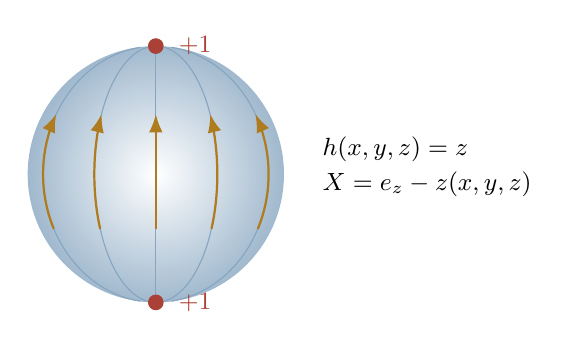
\begin{tikzpicture}[>=Latex,font=\small,line cap=round,scale=1.05]
 \shade[inner color=white,outer color=manifoldblue!43] (0,0) circle (1.55);
 \foreach \c in {-.88,-.48,0,.48,.88}
  \draw[manifoldblue!55,thin]
   plot[domain=8:172,samples=65,variable=\t]
    ({1.55*\c*sin(\t)},{1.55*cos(\t)});
 \foreach \c in {-.88,-.48,0,.48,.88}
  \draw[->,manifoldgold!85!black,thick]
   plot[domain=115:62,samples=25,variable=\t]
    ({1.55*\c*sin(\t)},{1.55*cos(\t)});
 \fill[manifoldred] (0,1.55) circle (2.7pt);
 \fill[manifoldred] (0,-1.55) circle (2.7pt);
 \node[anchor=west,manifoldred] at (.16,1.55) {$+1$};
 \node[anchor=west,manifoldred] at (.16,-1.55) {$+1$};
 \node[anchor=west] at (1.9,.30) {$h(x,y,z)=z$};
 \node[anchor=west] at (1.9,-.12) {$X=e_z-z(x,y,z)$};
\end{tikzpicture}
\caption{Gradient wysokości na $S^2$
ma dwa zera: na biegunie dolnym
i górnym. Oba mają indeks $+1$,
więc suma indeksów i $\chi(S^2)$ są równe $2$.
Złote łuki pokazują rzuty trajektorii gradientu
w metryce standardowej: biegną po południkach od minimum
do maksimum. Promień rysunku jest tylko skalą graficzną.}
\label{fig:poincare-hopf-16}
\end{figure}

\begin{przyklad}[Sfera i torus]
Na $S^2$ gradient
funkcji wysokości
ma minimum i maksimum.
Lokalne macierze
pochodnej pola są
odpowiednio dodatnio
i ujemnie określone
w dwóch wymiarach,
ale oba wyznaczniki
są dodatnie:
$1+1=\chi(S^2)=2$.
Na torusie $T^2$
istnieje nigdzie
nieznikające pole
styczne wzdłuż
jednego czynnika
$S^1$, więc
$e(TT^2)=0$ i
$\chi(T^2)=0$.
To dopowiada topologiczną
treść wzoru
Gaussa--Bonneta z
Rozdziału~\ref{ch:krzywizna}.
\end{przyklad}

\section{Forma przecięcia i przygotowanie do chirurgii}
\label{sec:forma-przeciecia-16}

Gdy $n=2k$, dwie
$k$-podrozmaitości
przecinają się
w punktach.
Ich liczba przecięcia
tworzy na środkowej
homologii formę
dwuliniową. Część
torsyjna nie jest
wykrywana przez
wartości całkowite
tej formy, więc
najpierw ją usuwamy.

\begin{twierdzenie}[Forma przecięcia]
\label{thm:forma-przeciecia-16}
Dla zamkniętej
zorientowanej
$M^{2k}$ parowanie
\[
 Q_M:
 \frac{H_k(M;\Z)}{\mathrm{Tor}}
 \times
 \frac{H_k(M;\Z)}{\mathrm{Tor}}
   \longrightarrow\Z,
 \qquad
 Q_M(a,b)=
 \langle\operatorname{PD}^{-1}(a)
 \smile\operatorname{PD}^{-1}(b),[M]\rangle
\]
jest \emph{unimodularne}, czyli doskonałe nad $\Z$:
macierz w dowolnej bazie
części wolnej ma wyznacznik
$\pm1$. Ponadto
$Q_M(a,b)=(-1)^kQ_M(b,a)$.
W wymiarze $4m$ forma
jest symetryczna, a
w wymiarze $4m+2$
antysymetryczna.
\end{twierdzenie}
\begin{proof}
Z dualności Poincarégo
otrzymujemy
$H_k(M;\Z)\cong H^k(M;\Z)$.
Twierdzenie o
współczynnikach
uniwersalnych daje
ciąg dokładny
\[
0\longrightarrow
 \operatorname{Ext}
     (H_{k-1}(M),\Z)
 \longrightarrow H^k(M;\Z)
 \longrightarrow
 \operatorname{Hom}(H_k(M),\Z)
 \longrightarrow0.
\]
Grupy homologii
zwartej triangulacji
są skończenie
generowane.
Składnik $\operatorname{Ext}$
jest więc torsyjny,
a grupa $\operatorname{Hom}$
jest dualną kratą
części wolnej $H_k$.
Po podzieleniu przez
torsję otrzymujemy
izomorfizm
\[
 H_k(M)/\mathrm{Tor}
 \ \cong\
 \operatorname{Hom}
    (H_k(M)/\mathrm{Tor},\Z).
\]
Dla wybranej konwencji kapowej ten izomorfizm
wysyła $a$ na funkcjonał
\[
 b\longmapsto\langle\operatorname{PD}^{-1}(a),b\rangle
 =Q_M(b,a)=(-1)^kQ_M(a,b).
\]
Wspólny czynnik $(-1)^k$ nie zmienia odwracalności.
Klasy torsyjne nie wpływają na $Q_M$, ponieważ
ich całkowita ewaluacja jest torsyjną liczbą całkowitą,
a więc zerem. Definicja na ilorazie jest zatem jednoznaczna.
Macierz odwzorowania
między wolną grupą
abelową a jej dualną
jest odwracalna nad
$\Z$, stąd jej
wyznacznik to $\pm1$.
Dla wszystkich klas, także niereprezentowanych
przez zanurzone podrozmaitości, przemienność
stopniowana iloczynu kubkowego daje znak
$(-1)^{k^2}=(-1)^k$. To dowodzi obu symetrii.
Nie zakładamy, że każda całkowita klasa homologii
ma reprezentanta będącego podrozmaitością.
\end{proof}

\begin{przyklad}
Na $S^2\times S^2$
w bazie
$[S^2\times\{p\}]$,
$[\{q\}\times S^2]$
forma ma macierz
\[
 Q=
 \begin{pmatrix}
  0&1\\1&0
 \end{pmatrix},
 \qquad\det Q=-1.
\]
Na torusie
$H_1(T^2)=\Z^2$
i w bazie dwóch
podstawowych okręgów
otrzymujemy
$\begin{psmallmatrix}
0&1\\-1&0
\end{psmallmatrix}$.
Druga forma jest
antysymetryczna,
bo oba cykle mają
wymiar nieparzysty.
\end{przyklad}

\begin{definicja}[Elementarna operacja chirurgiczna]
\index{elementarna operacja chirurgiczna@Elementarna operacja chirurgiczna}
\label{def:chirurgia-zarys-16}
Niech $0\leq k\leq n-1$
i niech dane będzie
\emph{obramowane}
zanurzenie
$S^k\times D^{\,n-k}
\hookrightarrow M^n$.
Elementarna
\emph{chirurgia indeksu $k$} (w przyjętej tutaj
konwencji: wymiar operowanej sfery; uchwyt w jej
śladzie ma indeks $k+1$) polega na usunięciu
wnętrza tego
otoczenia i
wklejeniu
$D^{k+1}\times
S^{\,n-k-1}$
wzdłuż wspólnego brzegu
\[
 \partial(S^k\times D^{n-k})
 =S^k\times S^{n-k-1}
 =\partial(D^{k+1}\times S^{n-k-1}).
\]
Dla ustalonego obramowanego zanurzenia sklejamy
punkty o tych samych współrzędnych produktowych na
$S^k\times S^{n-k-1}$; jest to określony dyfeomorfizm
brzegów. Jego dowolna dodatkowa zmiana jest dodatkową
daną i może zmienić wynik. Kołnierze określają gładką
strukturę przy szwie. Jeśli chcemy zachować orientację,
identyfikacja musi odwracać orientacje indukowane
na brzegach obu sklejanych części.
\end{definicja}

To wyjaśnia rolę
wcześniejszych tematów.
Twierdzenie o otoczeniu
tubularnym zapewnia
obszar, który można
wyciąć. Obramowanie
z Definicji~\ref{def:obramowanie-normalne}
pozwala zapisać go
jako \emph{iloczyn}
$S^k\times D^{n-k}$.
Klasy charakterystyczne
mogą wykazać, że
normalna wiązka
nie ma takiego
obramowania.
Forma przecięcia
kontroluje, jak
cykle środkowego
wymiaru są ze sobą
powiązane; po
operacji trzeba
obliczyć ją na nowo.
Szczegółowa teoria
sklejania, uchwytów
i zmian homologii
będzie osobnym
rozdziałem.

\begin{przyklad}[Cięcie sfery w dwóch punktach]
Na $S^2$ wybierzmy
dwa rozłączne
małe dyski:
$S^0\times D^2$
to właśnie ich suma.
Po wycięciu wnętrz
pozostaje walec
$S^1\times[0,1]$.
W chirurgii
$k=0,n=2$
dołączamy
$D^1\times S^1$,
drugi walec,
wzdłuż dwóch
brzegowych okręgów.
Wybieramy sklejenia zgodne z orientacją powstałej
powierzchni, czyli odwracające orientacje jej brzegów.
Wtedy dwa walce składają się w zorientowaną zamkniętą
powierzchnię rodzaju jeden, czyli torus. Bez tego
warunku sklejenie może dać butelkę Kleina:
po obejściu podłużnego okręgu kierunek poprzeczny
wraca wówczas z przeciwną orientacją. Sama
charakterystyka Eulera nie rozróżnia tych wyników.
Na poziomie
charakterystyki
Eulera: ze sfery
o $\chi=2$ usunięcie
dwóch dysków
odejmuje $2$,
a dołączenie walca nie zmienia wyniku:
$\chi(A\cup B)=\chi(A)+\chi(B)-\chi(A\cap B)$,
przy czym zarówno walec, jak i dwa okręgi sklejenia
mają charakterystykę $0$.
Torus ma więc
$\chi=0$, zgodnie
z bezpośrednim
obliczeniem.
\end{przyklad}

\par\smallskip
{\footnotesize\noindent\emph{Dalsza lektura:}
\href{https://pi.math.cornell.edu/~hatcher/AT/AT.pdf}{A.\ Hatcher, \emph{Algebraic Topology}, dualność i iloczyn kubkowy},
\href{https://pi.math.cornell.edu/~hatcher/VBKT/VB.pdf}{A.\ Hatcher, \emph{Vector Bundles and K-Theory}, sklejanie i klasy charakterystyczne},
\href{https://math.stanford.edu/~ralph/bookR4.pdf}{R.\ Cohen, \emph{Bundles, Manifolds, and Homotopy}, przecięcia i klasa Thoma}.\par}

\chapter{Teoria Morse'a: punkty krytyczne, uchwyty i przepływ}
\label{ch:teoria-morsea}
\index{teoria Morse'a}

Funkcja wysokości pozwala oglądać rozmaitość
po jednej poziomicy naraz. Między jej wartościami
krytycznymi nic istotnego się nie zmienia:
Twierdzenie~\ref{thm:pas-bez-krytycznych-15}
identyfikuje taki pas z iloczynem.
Wartość krytyczna jest chwilą, w której
pojawia się nowa część przestrzeni, otwór
albo zamknięcie otworu. Teoria Morse'a
zamienia ten obraz w twierdzenia o uchwytach
i homologiach. Na końcu poznamy trajektorie
gradientowe, które pozwalają obliczać różniczkę
kompleksu Morse'a.

W głównej części rozdziału $M^n$ jest gładką
rozmaitością \emph{zwartą bez brzegu}, a $f:M\to\R$
funkcją Morse'a. Definicję hesjanu
i niezdegenerowania podaliśmy w
Definicji~\ref{def:morse-pochodna}; istnienie
funkcji Morse'a i możliwość rozdzielenia
ich wartości krytycznych dowiedliśmy w
Twierdzeniu~\ref{thm:gestosc-morse}.
Zatem nie będziemy drugi raz udowadniać
tych samych faktów. Oznaczamy
\[
 M^a:=f^{-1}((-\infty,a]),\qquad
 \operatorname{Crit}_k(f)
  :=\{p:\dd f_p=0,\ \lambda(p)=k\},
 \qquad c_k:=\#\operatorname{Crit}_k(f).
\]
Przy wartości regularnej $a$ zbiór $M^a$
jest zwartą rozmaitością z brzegiem
$f^{-1}(a)$, o ile nie jest pusty.

\section{Lemat Morse'a: dokładny opis w pobliżu punktu}
\label{sec:lemat-morsea-17}

Hesjan w punkcie krytycznym mierzy
drugorzędową zmianę $f$. Jego indeks
$\lambda(p)$, wprowadzony przy
transwersalności w
Sekcji~\ref{sec:transwersalnosc-smale},
jest liczbą ujemnych kierunków.
Lemat Morse'a mówi znacznie więcej
niż wzór Taylora z resztą: po gładkiej
zmianie współrzędnych \emph{reszta znika}.

\begin{twierdzenie}[Lemat Morse'a]
\label{thm:lemat-morsea-17}
Jeśli $p$ jest niezdegenerowanym punktem
krytycznym o indeksie $\lambda$, istnieje
mapa $(u,v)$ wokół $p$, w której
$u\in\R^\lambda$, $v\in\R^{n-\lambda}$,
$p=(0,0)$ i
\begin{equation}\label{eq:postac-morsea-17}
 f(u,v)=f(p)-|u|^2+|v|^2.
\end{equation}
Liczba $\lambda$ nie zależy od mapy.
\end{twierdzenie}
\begin{proof}
Wybierzmy dowolne współrzędne $x$ z $x(p)=0$.
Ponieważ $\dd f_0=0$, liniowa zamiana
współrzędnych, twierdzenie Sylvestera
i przeskalowanie osi pozwalają założyć
\[
 \tfrac12\operatorname{Hess}_0f
  =J:=\operatorname{diag}(-I_\lambda,I_{n-\lambda}).
\]
Nie wolno jednak na tym poprzestać:
forma w punkcie $0$ nie opisuje jeszcze
całej funkcji w sąsiedztwie.
Dwukrotne całkowanie po odcinku
$t\mapsto tx$ daje \emph{dokładną} równość
\[
 f(x)-f(0)
  =x^{\mathsf T}H(x)x,\qquad
 H(x)=\int_0^1(1-t)\,
                    \operatorname{Hess}_{tx}f\,\dd t.
\]
Macierz $H(x)$ zależy gładko od $x$,
jest symetryczna i $H(0)=J$.
Rozbijmy $x=(x_-,x_+)$ i zapiszmy
\[
 H(x)=
 \begin{pmatrix} A(x)&B(x)\\
                 B(x)^{\mathsf T}&C(x)\end{pmatrix}.
\]
Blisko zera $A$ jest ujemnie określona,
a dopełnienie Schura
$S=C-B^{\mathsf T}A^{-1}B$ dodatnio
określone. Istotnie, w zerze mamy
$A=-I$, $B=0$, $S=I$, a określoność
jest własnością otwartą.
Uzupełniamy kwadrat, nie pomijając
zależności macierzy od $x$:
\[
 x^{\mathsf T}Hx
 =(x_-+A^{-1}Bx_+)^{\mathsf T}
       A(x_-+A^{-1}Bx_+)
   +x_+^{\mathsf T}Sx_+.
\]
Dodatnio określone macierze $-A$ i $S$
mają gładko zależne od $x$ dodatnie
pierwiastki kwadratowe. Blisko $I$
można je zbudować z szeregu potęgowego
$\sqrt{I+E}
 =I+\tfrac12E-\tfrac18E^2+\cdots$;
na mniejszym otoczeniu $\|E\|\leq q<1$.
Po dowolnej ustalonej liczbie różniczkowań
wyrazy są ograniczone przez wielomian
w numerze wyrazu razy potęgę $q$.
Szeregi pochodnych są więc lokalnie
jednostajnie zbieżne, co uzasadnia gładkość. Kładziemy
\[
 u=(-A)^{1/2}(x_-+A^{-1}Bx_+),
 \qquad v=S^{1/2}x_+.
\]
Otrzymujemy~\eqref{eq:postac-morsea-17}.
W zerze różniczka zmiany
$x\mapsto(u,v)$ jest identycznością,
bo $A(0)=-I$, $B(0)=0$, $S(0)=I$.
Twierdzenie o funkcji odwrotnej
czyni więc $(u,v)$ współrzędnymi
na pewnym otoczeniu $p$.
Przy $\lambda=0$ pomijamy blok $A$ i bierzemy
$v=H(x)^{1/2}x$; przy $\lambda=n$ bierzemy
$u=(-H(x))^{1/2}x$. Nie odwracamy w tych
przypadkach żadnego nieistniejącego bloku.

Na końcu trzeba sprawdzić jednoznaczność
liczby $\lambda$: hesjan w tych
współrzędnych ma macierz
$\operatorname{diag}(-2I_\lambda,2I_{n-\lambda})$,
a prawo bezwładności Sylvestera
zachowuje liczbę ujemnych kwadratów
przy każdej odwracalnej zmianie bazy.
\end{proof}

\begin{przyklad}[Trzy lokalne kształty w wymiarze dwa]
Na płaszczyźnie funkcje $x^2+y^2$,
$-x^2+y^2$ i $-x^2-y^2$ mają
odpowiednio indeksy $0,1,2$.
Pierwsza tworzy nową składową
podpoziomicy. Przy siodle dwie
części poziomicy stykają się
i zmieniają sposób połączenia.
Ostatnia może wypełnić ostatni
brzeg powierzchni. Sam rysunek
poziomic nie wyznacza jeszcze
globalnego wyniku: o sposobie
przyklejenia decyduje wcześniejsza
część rozmaitości.
\end{przyklad}

\begin{figure}[htbp]
\centering
\begin{tikzpicture}[>=Latex,line cap=round,font=\small,scale=.94]
 \begin{scope}[shift={(-4.15,0)}]
  \fill[gray!5] (0,0) circle (1.35);
  \fill[manifoldblue!40] (0,0) circle (.68);
  \draw[manifoldblue!85!black,very thick] (0,0) circle (.68);
  \draw[gray!50] (0,0) circle (1.35);
  \draw[->,manifoldgold!85!black,thick] (.79,.14)--(1.18,.21);
  \draw[->,manifoldgold!85!black,thick] (-.79,-.14)--(-1.18,-.21);
  \fill[manifoldred] (0,0) circle (2.5pt);
  \node at (0,-1.68) {minimum $\lambda=0$};
  \node[manifoldblue!75!black] at (0,-2.10) {pojawia się dysk};
 \end{scope}
 \begin{scope}
  \begin{scope}
   \clip (0,0) circle (1.35);
   \fill[gray!5] (-1.5,-1.5) rectangle (1.5,1.5);
   \fill[manifoldblue!40] (1.5,-1.5)--(1.5,1.5)
     -- plot[domain=1.5:-1.5,samples=50]
        ({sqrt(\x*\x+.15)},{\x}) -- cycle;
   \fill[manifoldblue!40] (-1.5,-1.5)--(-1.5,1.5)
     -- plot[domain=1.5:-1.5,samples=50]
        ({-sqrt(\x*\x+.15)},{\x}) -- cycle;
   \draw[manifoldgold!85!black,dashed,thick]
     (-1.38,-1.38)--(1.38,1.38)
     (-1.38,1.38)--(1.38,-1.38);
   \foreach \sgn in {-1,1}
    \draw[manifoldblue!85!black,very thick,
          domain=-1.4:1.4,samples=50]
      plot ({\sgn*sqrt(\x*\x+.15)},{\x});
  \end{scope}
  \draw[gray!50] (0,0) circle (1.35);
  \fill[manifoldred] (0,0) circle (2.5pt);
  \node at (0,-1.68) {siodło $\lambda=1$};
  \node[manifoldblue!75!black] at (0,-2.10) {dwa obszary};
 \end{scope}
 \begin{scope}[shift={(4.15,0)}]
  \fill[manifoldblue!40] (0,0) circle (1.35);
  \fill[white] (0,0) circle (.68);
  \draw[manifoldred!80!black,very thick] (0,0) circle (.68);
  \draw[gray!50] (0,0) circle (1.35);
  \draw[->,manifoldgold!85!black,thick] (1.18,.21)--(.79,.14);
  \draw[->,manifoldgold!85!black,thick] (-1.18,-.21)--(-.79,-.14);
  \fill[manifoldred] (0,0) circle (2.5pt);
  \node at (0,-1.68) {maksimum $\lambda=2$};
  \node[manifoldblue!75!black] at (0,-2.10) {otwór się zamyka};
 \end{scope}
\end{tikzpicture}
\caption{Lokalne podpoziomice trzech postaci
z lematu Morse'a w wymiarze dwa. Kolor niebieski
oznacza $f\leq a$: przy minimum pokazujemy $a>f(p)$,
a przy siodle i maksimum $a<f(p)$. Złote strzałki
wskazują wzrost $f$: od minimum na zewnątrz,
do maksimum ku środkowi. Przerywane proste
przy siodle to poziom krytyczny.}
\label{fig:poziomice-morse-17}
\end{figure}

\section{Przekroczenie wartości krytycznej: uchwyt}
\label{sec:uchwyt-morse-17}

Przedział bez wartości krytycznych mamy już
opisany w Twierdzeniu~\ref{thm:pas-bez-krytycznych-15}.
Teraz $a<b$ są wartościami regularnymi,
a w $f^{-1}([a,b])$ leży dokładnie jeden
punkt krytyczny $p$ z $a<f(p)=c<b$ i indeksem
$\lambda$. Dla przejrzystości
piszemy $D^0=\{\mathrm{punkt}\}$
i $S^{-1}=\varnothing$.

\begin{definicja}[Uchwyt indeksu $\lambda$]
\label{def:uchwyt-morse-17}
$n$-wymiarowy \emph{uchwyt indeksu $\lambda$}
to $H_\lambda=D^\lambda\times D^{n-\lambda}$.
Jego część przyczepiana to
$S^{\lambda-1}\times D^{n-\lambda}$.
Rdzeń $D^\lambda\times\{0\}$ ma
wymiar $\lambda$, a dysk
$\{0\}\times D^{n-\lambda}$ biegnie
w kierunkach poprzecznych.
Przyklejamy uchwyt do brzegu
dotychczasowej podpoziomicy
przez zanurzenie jego części przyczepianej.
\end{definicja}

\begin{twierdzenie}[Dołączenie uchwytu Morse'a]
\label{thm:uchwyt-morse-17}
W powyższej sytuacji $M^b$ powstaje,
z dokładnością do zaokrąglenia naroży
i dyfeomorfizmu, z $M^a$ przez
dołączenie uchwytu $H_\lambda$.
W szczególności istnieje odwzorowanie
$S^{\lambda-1}\to M^a$ takie, że
\begin{equation}\label{eq:komorka-morse-17}
 M^b\simeq M^a\cup_{S^{\lambda-1}}D^\lambda,
 \qquad
 H_j(M^b,M^a;\Z)\cong
 \begin{cases}\Z,&j=\lambda,\\0,&j\ne\lambda.
 \end{cases}
\end{equation}
Przy $\lambda=0$ pojawia się składowa;
przy $\lambda=n$ dołącza się
$n$-wymiarowy dysk wzdłuż całej
jego sfery brzegowej.
\end{twierdzenie}
\begin{proof}
\emph{Krok 1: ograniczamy pas.}
Na częściach $[a,c-\varepsilon]$
i $[c+\varepsilon,b]$ nie ma
punktów krytycznych.
Przepływ pola $\nabla f/|\nabla f|^2$
z Twierdzenia~\ref{thm:pas-bez-krytycznych-15}
identyfikuje te pasy z iloczynami.
Wystarczy więc zrozumieć
$f^{-1}([c-\varepsilon,c+\varepsilon])$
dla małego $\varepsilon>0$.

\emph{Krok 2: uchwyt z właściwą częścią przyczepianą.}
W mapie Morse'a mamy $f-c=-|u|^2+|v|^2$.
Wybierzmy $\varepsilon>0$ i $0<r^2<\varepsilon$
tak małe, by poniższy zbiór mieścił się w mapie:
\[
 H=\{(u,v): |v|\leq r,\quad |u|^2\leq\varepsilon+|v|^2\}.
\]
Odwzorowanie
\[
 (a,b)\longmapsto
 \bigl(\sqrt{\varepsilon+r^2|b|^2}\,a,rb\bigr)
 \quad (|a|\leq1,\ |b|\leq1)
\]
jest dyfeomorfizmem $D^\lambda\times D^{n-\lambda}$ na $H$.
Ponadto $H\subset\operatorname{int}M^{c+\varepsilon}$ oraz
\[
 H\cap M^{c-\varepsilon}
 =\{|u|^2=\varepsilon+|v|^2,\ |v|\leq r\}.
\]
Jest to dokładnie obraz $S^{\lambda-1}\times D^{n-\lambda}$;
przy $\lambda=0$ przecięcie jest puste.
Rdzeń $v=0$ ma brzeg w poziomicy $c-\varepsilon$.
Tak zdefiniowana część przyczepiana już leży na właściwym
poziomie; nie trzeba przesuwać jej z płaskiej ściany pudełka.

\emph{Krok 3: dopełnienie jest kołnierzem.}
Wybierzmy metrykę euklidesową na otoczeniu $H$,
przedłużoną podziałem jedności na $M$.
Dla $X=-\nabla f$ mamy tam
\[
 \dot u=2u,\quad\dot v=-2v,\qquad
 (u(t),v(t))=(e^{2t}u(0),e^{-2t}v(0)).
\]
Niech $L=M^{c-\varepsilon}\cup H$.
Blisko naroża jego dopełnienie opisują nierówności
$F=f-(c-\varepsilon)>0$ i $G=|v|^2-r^2>0$.
Na obu ścianach pole jest skierowane do $L$, ponieważ
\[
 XF=-4(|u|^2+|v|^2)<0,\qquad XG=-4|v|^2<0.
\]
Możemy zatem zaokrąglić naroże, zachowując poprzeczność
i ten sam kierunek pola: w płaszczyźnie $(F,G)$
zastępujemy narożnik gładkim łukiem o normalnej
będącej dodatnią kombinacją normalnych obu ścian.
Zaokrąglenie wybieramy na zewnątrz $L$, małe i wewnątrz
$M^{c+\varepsilon}$, tak by zachować $M^{c-\varepsilon}\subset L'$.
Otrzymaną rozmaitość oznaczmy przez $L'$.
Punkt $p$ leży w jej wnętrzu.

Zbiór $K=M^{c+\varepsilon}\setminus\operatorname{int}L'$
jest zwarty i nie zawiera punktów krytycznych.
Stąd $-Xf\geq m>0$ na $K$.
Każda trajektoria z górnego brzegu dociera do $\partial L'$
w skończonym czasie: inaczej $f$ malałaby co najmniej
z prędkością $m$ w zbiorze, na którym jest ograniczona.
W odwrotnym czasie każda trajektoria z $\partial L'$
dociera do górnego brzegu. Nie może powtórnie przeciąć
$\partial L'$, bo $X$ jest tam ściśle skierowane do środka.
Czas trafienia jest gładki na mocy twierdzenia
o funkcji uwikłanej i poprzeczności.
Przeskalowanie czasu na każdej trajektorii daje
$K\cong\partial L'\times[0,1]$.
Wchłonięcie tego kołnierza dowodzi tezy o uchwycie.
Przy $\lambda=n$ nie ma ściany $|v|=r$;
cały brzeg $H=D^n$ przykleja się do dolnej podpoziomicy.
Zamknięte składowe $L'$ nie wymagają żadnego kołnierza.

\emph{Krok 4: komórka i homologia względna.}
Oznaczmy odwzorowanie przyczepienia przez $\alpha(a,b)$.
Homotopia $\alpha(a,(1-t)b)$ zastępuje je odwzorowaniem
zależnym tylko od $a\in S^{\lambda-1}$.
Dołączenia po homotopijnych odwzorowaniach mają ten sam typ
homotopijny pary: homotopię realizuje walec na części
przyczepianej, który wchłaniamy w jej kołnierz.
Po tej zmianie skurczenie czynnika $D^{n-\lambda}$
daje dołączenie samego rdzenia $D^\lambda$.
Nie jest to skurczenie pierwotnego uchwytu
przy jednoczesnym punktowym unieruchomieniu jego całej
części przyczepianej.
Kołnierze pozwalają zastosować wycięcie
(najpierw pogrubiamy część przyczepianą), skąd
\[
 H_j(M^b,M^a;\Z)
 \cong H_j(H_\lambda,S^{\lambda-1}\times D^{n-\lambda};\Z)
 \cong H_j(D^\lambda,S^{\lambda-1};\Z).
\]
Homologia tej pary jest $\Z$ w stopniu $\lambda$
i zerem w pozostałych stopniach, także dla
$(D^0,S^{-1})=(\{\mathrm{punkt}\},\varnothing)$.
\end{proof}

\begin{figure}[htbp]
\centering
\begin{tikzpicture}[>=Latex,font=\small,line cap=round,line join=round]
 \tikzset{old/.style={draw=manifoldblue!80!black,thick,fill=manifoldblue!22},
          new/.style={draw=manifoldgold!85!black,thick,fill=manifoldgold!38},
          seam/.style={manifoldred!80!black,thick,densely dashed},
          pair/.pic={
           \path[old] (-.4,.45)--(-.9,.45)
             arc[start angle=90,end angle=270,radius=.45]
             --(-.4,-.45)--cycle;
           \path[old] (.4,-.45)--(.9,-.45)
             arc[start angle=270,end angle=450,radius=.45]
             --(.4,.45)--cycle;
          },
          ring/.pic={
           \path[old,even odd rule] (0,0) circle (.8) (0,0) circle (.36);
          }}
 \node[font=\bfseries] at (-2.1,3.1) {przed};
 \node[font=\bfseries] at (2.1,3.1) {po};
 \foreach \y in {2.05,0,-2.25}
    \draw[->,gray!70,thick] (-.35,\y)--(.35,\y);
 \node[anchor=east,align=right] at (-3.65,2.05)
    {$0$-uchwyt\\nowa składowa};
 \node[gray!65,font=\Large] at (-2.1,2.05) {$\varnothing$};
 \path[new] (2.1,2.05) circle (.66);
 \draw[gray!22] (-5.1,1.05)--(3.6,1.05);
 \node[anchor=east,align=right] at (-3.65,0)
    {$1$-uchwyt\\połączenie składowych};
 \path (-2.1,0) pic {pair};
 \path (2.1,0) pic {pair};
 \path[new] (1.7,-.45) rectangle (2.5,.45);
 \draw[seam] (1.7,-.45)--(1.7,.45) (2.5,-.45)--(2.5,.45);
 \node[manifoldgold!75!black] at (2.1,-.77) {$D^1\times D^1$};
 \draw[gray!22] (-5.1,-1.2)--(3.6,-1.2);
 \node[anchor=east,align=right] at (-3.65,-2.25)
    {$2$-uchwyt\\wypełnienie otworu};
 \path (-2.1,-2.25) pic {ring};
 \path (2.1,-2.25) pic {ring};
 \path[new] (2.1,-2.25) circle (.36);
 \draw[seam] (2.1,-2.25) circle (.36);
\end{tikzpicture}
\caption{Trzy niezależne przykłady dla dwuwymiarowej
podpoziomicy, pokazane z góry. Niebieski oznacza
część istniejącą, złoty nowy uchwyt, a czerwone
przerywane odcinki lub okrąg --- część przyczepianą.
W drugim wierszu prostokąt przykleja się dokładnie
do dwóch odcinków brzegu. Inne przyklejenie $1$-uchwytu
może utworzyć otwór zamiast połączyć składowe.}
\label{fig:uchwyty-morse-17}
\end{figure}

\begin{przyklad}[Wysokość na sferze]
\label{prz:morse-sfera-17}
Na jednostkowej sferze $S^2\subset\R^3$
weźmy $f(x,y,z)=z$. Krytyczne są
tylko biegun południowy i północny.
Przy południowym
$z=-\sqrt{1-x^2-y^2}
 =-1+\tfrac12(x^2+y^2)+O(|(x,y)|^4)$,
więc indeks wynosi $0$.
Przy północnym znak formy
kwadratowej jest przeciwny,
więc indeks wynosi $2$.
Najpierw pojawia się dysk,
między biegunami podpoziomice
są dyskami, a po przejściu przez
biegun północny dołączamy
$2$-uchwyt. Dostajemy
$c_0=c_2=1$, $c_1=0$.
\end{przyklad}

\begin{przyklad}[Lekko przechylona wysokość torusa]
\label{prz:morse-torus-17}
Standardowy torus parametryzujemy przez
\[
 ((R+r\cos\theta)\cos\phi,\
  (R+r\cos\theta)\sin\phi,\
  r\sin\theta),\qquad R>r>0.
\]
Sama współrzędna $z=r\sin\theta$
ma \emph{okręgi} punktów krytycznych:
nie jest funkcją Morse'a.
Weźmy zamiast niej
\[
 f=z+\varepsilon x
 =r\sin\theta+
    \varepsilon(R+r\cos\theta)\cos\phi,
 \qquad 0<\varepsilon<r/R.
\]
Warunek $\partial_\phi f=0$ daje
$\phi=0$ lub $\phi=\pi$, bo
$R+r\cos\theta>0$.
Warunek $\partial_\theta f=0$ ma
dwa rozwiązania przy każdej z tych
wartości $\phi$, jedno przy górze
i jedno przy dole torusa.
Można je zapisać jawnie. Niech $s=\cos\phi\in\{-1,1\}$,
$t=\operatorname{sgn}(\sin\theta)\in\{-1,1\}$ oraz
$L=\sqrt{1+\varepsilon^2}$ i $h=r/L$.
Równanie $\cos\theta=\varepsilon s\sin\theta$ daje
\[
 \sin\theta=\frac{t}{L},\qquad
 \cos\theta=\frac{\varepsilon st}{L},\qquad
 (x,y,z)=(sR+t\varepsilon h,\,0,\,th).
\]
Wartość funkcji w tym punkcie wynosi
$f=\varepsilon sR+trL$. Te same współrzędne wykorzystano
do umieszczenia znaczników na Rysunku~\ref{fig:torus-morse-17}.
W tych punktach mieszana pochodna
wynosi zero, a na przekątnej hesjanu
stoją
\[
 f_{\theta\theta}
  =-r(\sin\theta+
       \varepsilon\cos\theta\cos\phi),
 \qquad
 f_{\phi\phi}
  =-\varepsilon(R+r\cos\theta)\cos\phi.
\]
Pierwsza jest ujemna u góry
i dodatnia u dołu; druga jest
ujemna dla $\phi=0$
i dodatnia dla $\phi=\pi$.
Zatem indeksy czterech punktów
to kolejno $0,1,1,2$.
Ich wartości, od najmniejszej
do największej, wynoszą
\[
 -r\sqrt{1+\varepsilon^2}-\varepsilon R,\quad
 -r\sqrt{1+\varepsilon^2}+\varepsilon R,\quad
 r\sqrt{1+\varepsilon^2}-\varepsilon R,\quad
 r\sqrt{1+\varepsilon^2}+\varepsilon R.
\]
Nierówność $\varepsilon R<r$
zapewnia tę kolejność.
Podpoziomica jest kolejno:
dyskiem, pierścieniem,
torusem z usuniętym dyskiem
i całym torusem. To są
dołączenia uchwytów indeksów
$0,1,1,2$. Sposób przyklejenia
drugiego $1$-uchwytu rozstrzyga,
że powstaje rodzaj $1$.
\end{przyklad}

\begin{figure}[htbp]
\centering
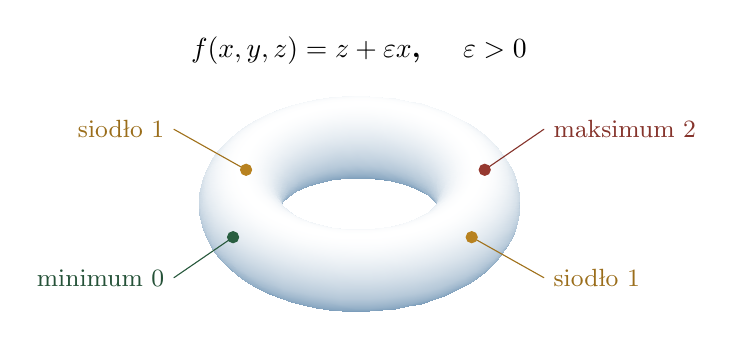
\begin{tikzpicture}[>=Latex,font=\small,line cap=round]
 \node[font=\bfseries] at (0,1.94)
   {$f(x,y,z)=z+\varepsilon x$, \quad $\varepsilon>0$};
  % Przykladowe epsilon spelnia epsilon R<r; punkty liczymy z df=0.
  \pgfmathsetmacro{\morseeps}{0.16}
  \pgfmathsetmacro{\morseh}{0.69/sqrt(1+\morseeps*\morseeps)}
  \pgfmathsetmacro{\morserplus}{2+\morseeps*\morseh}
  \pgfmathsetmacro{\morserminus}{2-\morseeps*\morseh}
  \begin{axis}[hide axis,view={0}{34},axis equal image,clip=false,scale=2,
    xmin=-3,xmax=3,ymin=-3,ymax=3,zmin=-.8,zmax=.8,scale only axis,
    at={(0,0)},anchor=center,width=9cm,height=5cm,
     colormap={toruslight}{color(0cm)=(manifoldblue!67);
       color(.42cm)=(manifoldblue!33);color(1cm)=(white)}]
   \addplot3[surf,shader=interp,draw=none,z buffer=sort,
     samples=34,samples y=68,domain=0:360,y domain=0:360,
     variable=\t,variable y=\p]
    ({(2+0.69*cos(\t))*cos(\p)},
     {(2+0.69*cos(\t))*sin(\p)},
     {0.69*sin(\t)});
    \addplot3[only marks,mark=*,mark size=2pt,
      mark options={fill=manifoldgreen!75!black,draw=manifoldgreen!75!black}]
      coordinates {(-\morserplus,0,-\morseh)};
    \addplot3[only marks,mark=*,mark size=2pt,
      mark options={fill=manifoldgold!90!black,draw=manifoldgold!90!black}]
      coordinates {(-\morserminus,0,\morseh)};
    \addplot3[only marks,mark=*,mark size=2pt,
      mark options={fill=manifoldgold!90!black,draw=manifoldgold!90!black}]
      coordinates {(\morserminus,0,-\morseh)};
    \addplot3[only marks,mark=*,mark size=2pt,
      mark options={fill=manifoldred!88!black,draw=manifoldred!88!black}]
      coordinates {(\morserplus,0,\morseh)};
    % Punkty, prowadnice i etykiety korzystają z tej samej projekcji.
    \draw[manifoldgreen!70!black,thin]
      (axis cs:-\morserplus,0,-\morseh)--(axis cs:-3.1,0,-1.5)
      node[anchor=east,manifoldgreen!65!black] {minimum $0$};
    \draw[manifoldgold!78!black,thin]
      (axis cs:-\morserminus,0,\morseh)--(axis cs:-3.1,0,1.5)
      node[anchor=east,manifoldgold!75!black] {siodło $1$};
    \draw[manifoldgold!78!black,thin]
      (axis cs:\morserminus,0,-\morseh)--(axis cs:3.1,0,-1.5)
      node[anchor=west,manifoldgold!75!black] {siodło $1$};
    \draw[manifoldred!78!black,thin]
      (axis cs:\morserplus,0,\morseh)--(axis cs:3.1,0,1.5)
      node[anchor=west,manifoldred!78!black] {maksimum $2$};
  \end{axis}
\end{tikzpicture}
\caption{Torus o przekroju kołowym oglądany ukośnie z góry
($R=2$, $r=0{,}69$, $\varepsilon=0{,}16$).
Znaczniki pokazują rzuty wszystkich czterech punktów krytycznych,
także gdy powierzchnia torusa je przesłania. Punkty te mają
indeksy $0,1,1,2$; składnik $\varepsilon x$
rozdziela ich wartości. Podpoziomice są kolejno
dyskiem, pierścieniem, torusem bez dysku i całym
torusem.}
\label{fig:torus-morse-17}
\end{figure}

\section{Komórki, nierówności Morse'a i twierdzenie Reeba}
\label{sec:nierownosci-morse-17}

Przykłady sfery i torusa pokazują, że
punkt krytyczny indeksu $\lambda$ może
dodać tylko \emph{jedną} komórkę wymiaru
$\lambda$. Nie znaczy to, że dodaje
niezależną klasę homologii:
komórka może zabić wcześniejszy cykl.
To właśnie mierzy jej brzeg w kompleksie
komórkowym z
Rozdziału~\ref{ch:homologia-przestrzeni}.

\begin{twierdzenie}[Model CW funkcji Morse'a]
\label{thm:cw-morse-17}
Rozmaitość $M$ ma typ homotopijny
skończonego kompleksu CW $K_f$
z dokładnie $c_k$ komórkami
wymiaru $k$. W szczególności
istnieje kompleks wolnych grup
abelowych
\[
 0\longrightarrow C_n
 \xrightarrow{\partial_n}C_{n-1}
 \longrightarrow\cdots
 \xrightarrow{\partial_1}C_0
 \longrightarrow0,\qquad
 C_k\cong\Z^{c_k},
\]
którego homologiami są $H_k(M;\Z)$.
Generator $C_k$ możemy oznaczyć
punktem krytycznym indeksu $k$.
\end{twierdzenie}
\begin{proof}
Na zwartej $M$ punktów krytycznych
jest skończenie wiele
(Twierdzenie~\ref{thm:gestosc-morse}).
Po małej perturbacji wartości
punktów krytycznych są różne;
wybieramy perturbację stałą
w ich małych otoczeniach,
więc punkty i ich indeksy
pozostają te same, a poza
otoczeniami różniczka $f$
jest oddzielona od zera.
Wybieramy wartości
regularne
$a_0<a_1<\cdots<a_N$
tak, żeby między sąsiednimi
znajdował się dokładnie jeden
punkt krytyczny, a $M^{a_0}$
było puste i $M^{a_N}=M$.
Przy każdym przejściu
Twierdzenie~\ref{thm:uchwyt-morse-17}
zastępuje parę podpoziomic
dołączeniem jednej komórki
$D^{\lambda_i}$.

Wyjaśnijmy indukcję, ponieważ
równoważność homotopijna na
jednym etapie nie jest dosłownie
równością przestrzeni.
Jeśli zbudowany dotąd kompleks
$K_{i-1}$ jest homotopijnie
równoważny $M^{a_{i-1}}$,
przenosimy odwzorowanie
$S^{\lambda_i-1}\to M^{a_{i-1}}$
przez wybraną odwrotność
homotopijną do $K_{i-1}$.
Już na tym etapie stosujemy aproksymację komórkową:
odwzorowanie ze sfery $S^{\lambda_i-1}$ zastępujemy homotopijnym
odwzorowaniem do $(\lambda_i-1)$-szkieletu $K_{i-1}$.
Dzięki temu następne dołączenie rzeczywiście daje
kompleks CW, nawet jeśli starsze komórki mają większy wymiar.
Dla $\lambda_i=0$ po prostu dodajemy punkt.
Dołączenie komórki po odwzorowaniach
homotopijnych daje
homotopijnie równoważne
przestrzenie: homotopię
na sferze rozszerza się
na dołączony walec
$S^{\lambda_i-1}\times[0,1]$,
a następnie wchłania ten
walec w kołnierz dysku.
Tak powstaje $K_i$ z jedną
nową komórką.
Po ostatnim kroku
$K_N\simeq M$.
Złożenie komórek daje
kompleks łańcuchów CW;
ich liczby w każdym stopniu
to dokładnie $c_k$.
\end{proof}

\begin{twierdzenie}[Słabe i mocne nierówności Morse'a]
\label{thm:nierownosci-morse-17}
Niech $b_k=\dim_{\mathbb F}H_k(M;\mathbb F)$
dla dowolnego ciała $\mathbb F$.
Wtedy $c_k\geq b_k$ oraz dla
$0\leq q<n$
\begin{equation}\label{eq:mocne-morse-17}
 \sum_{k=0}^q(-1)^{q-k}c_k
 \ \geq\
 \sum_{k=0}^q(-1)^{q-k}b_k.
\end{equation}
Na końcu otrzymujemy równość
\begin{equation}\label{eq:euler-morse-17}
 \chi(M)=\sum_{k=0}^n(-1)^kc_k.
\end{equation}
\end{twierdzenie}
\begin{proof}
Tensorujemy kompleks z poprzedniego
twierdzenia z $\mathbb F$.
Niech $r_k=\operatorname{rank}_{\mathbb F}
(\partial_k:C_k\otimes\mathbb F
\to C_{k-1}\otimes\mathbb F)$,
przy $r_0=r_{n+1}=0$.
Z twierdzenia o rzędzie i jądrze
\[
 \dim\ker\partial_k=c_k-r_k.
\]
Ponieważ $\partial_k\partial_{k+1}=0$,
obraz $\partial_{k+1}$ jest podprzestrzenią
tego jądra i ma wymiar $r_{k+1}$.
Stąd, \emph{bez pominiętego składnika},
\begin{equation}\label{eq:ranki-morse-17}
 b_k=c_k-r_k-r_{k+1},
 \qquad c_k=b_k+r_k+r_{k+1}.
\end{equation}
Wszystkie rzędy są nieujemne,
więc $c_k\geq b_k$.
Po przemnożeniu~\eqref{eq:ranki-morse-17}
przez $(-1)^{q-k}$ i zsumowaniu
od $0$ do $q$ składniki $r_k$
i $r_{k+1}$ skracają się parami.
Zostaje dokładnie
\[
 \sum_{k=0}^q(-1)^{q-k}(c_k-b_k)
   =r_{q+1}\geq0.
\]
To dowodzi~\eqref{eq:mocne-morse-17}.
Dla $q=n$ prawa strona wynosi
$r_{n+1}=0$. Pomnożenie
przez $(-1)^n$ daje
\eqref{eq:euler-morse-17},
bo $\chi(M)=\sum(-1)^kb_k$.
\end{proof}

\begin{przyklad}[Dolne ograniczenia i torsja]
Na $S^2$ mamy $(b_0,b_1,b_2)=(1,0,1)$;
wysokość z Przykładu~\ref{prz:morse-sfera-17}
realizuje dokładnie dwa niezbędne
punkty. Dla torusa
$(b_0,b_1,b_2)=(1,2,1)$,
a funkcja z
Przykładu~\ref{prz:morse-torus-17}
realizuje $(c_0,c_1,c_2)=(1,2,1)$.
Nierówności możemy stosować
nad różnymi ciałami: dla
$\R P^2$ współczynniki
$\mathbb F_2$ dają
$(b_0,b_1,b_2)=(1,1,1)$,
więc każda funkcja Morse'a
ma co najmniej trzy punkty
krytyczne. Nad $\Q$ środkowa
i najwyższa grupa znikają.
Różnica pokazuje, dlaczego
wybór współczynników może
ujawniać torsję, wspomnianą
już w
Rozdziale~\ref{ch:homologia-przestrzeni}.
\end{przyklad}

\begin{twierdzenie}[Twierdzenie Reeba o dwóch punktach]
\label{thm:reeb-morse-17}
Jeśli spójna zamknięta rozmaitość
$M^n$, $n\geq1$, ma funkcję
Morse'a z dokładnie dwoma
punktami krytycznymi, to
$M$ jest \emph{homeomorficzna}
z $S^n$.
\end{twierdzenie}
\begin{proof}
Minimum i maksimum istnieją,
więc są to oba punkty krytyczne;
ich indeksy wynoszą $0$ i $n$.
Lemat Morse'a daje małą
podpoziomicę wokół minimum
dyfeomorficzną z $D^n$ oraz
małą nadpoziomicę wokół maksimum
również dyfeomorficzną z $D^n$.
Pomiędzy nimi nie ma wartości
krytycznych, więc
Twierdzenie~\ref{thm:pas-bez-krytycznych-15}
przedstawia pas jako
$S^{n-1}\times[0,1]$.
Po wchłonięciu kołnierza
otrzymujemy dwie kopie $D^n$
sklejone wzdłuż brzegu
pewnym dyfeomorfizmem
$h:S^{n-1}\to S^{n-1}$.
Jako \emph{homeomorfizm}
$h$ przedłuża się radialnie
na dysk:
$H(ru)=r\,h(u)$ dla
$u\in S^{n-1}$, $r\in[0,1]$,
oraz $H(0)=0$.
To przedłużenie jest ciągłe
również w $0$, ma ciągłą
odwrotność zbudowaną z $h^{-1}$.
Zmieniając współrzędne
na jednym dysku przez $H$,
otrzymujemy standardowe
sklejenie dwóch półkul,
czyli $S^n$.
\end{proof}

\begin{uwaga}
Ostatni argument jest topologiczny.
Radialne przedłużenie $h$ nie musi być
gładkie w środku dysku, zatem dowód
nie pozwala zastąpić słowa
„homeomorficzna” przez
„dyfeomorficzna”. To rozróżnienie
będzie ważne przy egzotycznych
strukturach gładkich i chirurgii.
\end{uwaga}

\section{Gradient i rozmaitości trajektorii}
\label{sec:gradient-morse-17}

Metryka $g$ przekształca różniczkę
$\dd f$ w gradient $\nabla_g f$
(Definicja~\ref{def:gradient-dywergencja}).
Nie wybieramy jej po to, by zmieniać
punkty krytyczne: te zależą od $f$.
Metryka decyduje natomiast, którędy
biegną trajektorie pola
$X=-\nabla_g f$.
Na zwartej $M$ jego przepływ
$\Phi_t$ istnieje dla wszystkich
$t\in\R$.

\begin{stwierdzenie}[Spadek funkcji i końce trajektorii]
\label{prop:spadek-morse-17}
Dla każdej trajektorii $\gamma(t)=\Phi_t(x)$
\begin{equation}\label{eq:spadek-morse-17}
 \frac{\dd}{\dd t} f(\gamma(t))
 =-|\nabla_g f(\gamma(t))|_g^2\leq0.
\end{equation}
Jeżeli $\gamma$ nie jest stała, to
ma granice przy $t\to-\infty$
i $t\to+\infty$, będące
punktami krytycznymi.
\end{stwierdzenie}
\begin{proof}
Pierwsza równość to reguła łańcuchowa
i definicja gradientu:
$\dd f(-\nabla f)=-g(\nabla f,\nabla f)$.
Równość zachodzi tylko w punkcie
krytycznym; jeśli trajektoria
do niego dotrze w skończonym czasie,
jednoznaczność równania różniczkowego
sprawia, że była stała.
Ponieważ $f(M)$ jest ograniczone,
funkcja $t\mapsto f(\gamma(t))$
ma granice na obu końcach i
\[
 \int_0^\infty
       |\nabla f(\gamma(t))|^2\,\dd t
 =f(x)-\lim_{t\to\infty}f(\gamma(t))
 <\infty.
\]
Na zwartej $M$ pole i pochodna
funkcji $|\nabla f|^2$ są ograniczone,
więc $t\mapsto|\nabla f(\gamma(t))|^2$
jest jednostajnie ciągła.
Nieujemna jednostajnie ciągła
funkcja o skończonej całce na
$[0,\infty)$ dąży do zera:
gdyby przy nieskończenie wielu
chwilach była większa od $\eta>0$,
jednostajna ciągłość dawałaby
rozłączne przedziały stałej
dodatniej długości, na których
przekracza $\eta/2$, sprzeczne
ze skończonością całki.
Każdy punkt skupienia $\gamma(t)$
jest zatem krytyczny.

Zbiór graniczny jest przecięciem
malejących zwartych, spójnych
zbiorów
$\overline{\{\gamma(t):t\geq T\}}$,
więc jest spójny i niepusty.
Punktów krytycznych funkcji
Morse'a na zwartej $M$ jest
skończenie wiele; jedyny
spójny niepusty podzbiór
takiego zbioru to pojedynczy
punkt. Cała trajektoria
zbiega do niego. Dla
$t\to-\infty$ stosujemy
ten sam argument do $-X$.
\end{proof}

\begin{definicja}[Rozmaitości stabilna i niestabilna]
\index{rozmaitosci stabilna i niestabilna@Rozmaitości stabilna i niestabilna}
\label{def:stable-morse-17}
Dla punktu krytycznego $p$ kładziemy
\[
 W^s(p)=\{x:\lim_{t\to+\infty}\Phi_t(x)=p\},
 \qquad
 W^u(p)=\{x:\lim_{t\to-\infty}\Phi_t(x)=p\}.
\]
Litery $s,u$ pochodzą od
angielskich \emph{stable}, \emph{unstable}.
W kierunku przyszłości trajektorie
na $W^s$ zbiegają do $p$;
trajektorie na $W^u$ wychodzą z $p$
przy biegu czasu do przodu.
\end{definicja}

\begin{twierdzenie}[Wymiary rozmaitości stabilnych]
\label{thm:stable-morse-17}
Dla dowolnej gładkiej metryki $g$ rozmaitość
$W^u(p)$ jest różnowartościowo
immersowaną rozmaitością
dyfeomorficzną z $\R^{\lambda(p)}$,
a $W^s(p)$ z $\R^{n-\lambda(p)}$.
Ich przestrzenie styczne w $p$ są odpowiednio
dodatnią i ujemną przestrzenią spektralną $DX_p$.
Metrykę można ponadto wybrać euklidesową
w małych rozłącznych mapach Morse'a. W tych mapach
\[
 W^u_{\mathrm{loc}}(p)=\{v=0\},
 \qquad
 W^s_{\mathrm{loc}}(p)=\{u=0\}.
\]
\end{twierdzenie}
\begin{proof}
Ponieważ punktów krytycznych
jest skończenie wiele, bierzemy
rozłączne mapy z
Lematu~\ref{thm:lemat-morsea-17}
i gładkie funkcje odcinające
równe $1$ blisko ich środków.
Wypukłe połączenie
metryk euklidesowych w tych
mapach z dowolną metryką
globalną daje metrykę
euklidesową na mniejszych mapach.
Tam równania przepływu
i ich rozwiązania podaliśmy
w dowodzie
Twierdzenia~\ref{thm:uchwyt-morse-17}.
Warunek zbiegania do $(0,0)$
przy $t\to+\infty$ zmusza $u=0$,
bo $u(t)=e^{2t}u(0)$;
analogicznie zbieganie
przy $t\to-\infty$ zmusza $v=0$.
To dowodzi lokalnego opisu
i wymiarów.

Każdy $x\in W^s(p)$
po dostatecznie długim czasie
wpada do małego lokalnego
dysku $\{u=0\}$, a
$x=\Phi_{-T}(y)$
dla pewnego punktu $y$
tego dysku. Stąd
\[
 W^s(p)=\bigcup_{T\geq0}
      \Phi_{-T}(W^s_{\mathrm{loc}}(p)).
\]
Te obrazy są gładkimi kopiami
otwartego dysku i są
zagnieżdżone, jeśli lokalny
dysk wybierzemy niezmienniczy
przy przepływie naprzód.
Odwzorowania przejścia są
ograniczeniami dyfeomorfizmów
$\Phi_t$, więc określają
gładką strukturę na sumie.
Ustalmy w lokalnym dysku
kulę promienia $\delta$.
Każda trajektoria w
$W^s(p)\setminus\{p\}$
przecina jej sferę raz, gdy
wbiega do tej kuli: od tej
chwili lokalny wzór
$v(t)=e^{-2t}v(0)$
ściśle zmniejsza $|v|$.
Punkt takiej trajektorii
opisują kierunek na
$S^{n-\lambda(p)-1}$
i czas od przecięcia.
Jawna parametryzacja, dla $v\ne0$, to
\[
 v\longmapsto
 \Phi_{-\frac12\log(|v|/\delta)}
          (0,\delta v/|v|).
\]
Blisko zera jest to dokładnie $(0,v)$,
więc przedłuża się gładko przez $v=0$.
Jedyność przecięcia sfery i gładkość czasu trafienia
dają odwrotność, a więc standardową
strukturę $\R^{n-\lambda(p)}$.
Włączenie w $M$ jest
różnowartościową immersją.
Dla wymiaru zerowego
jest to po prostu $\{p\}$.
Dla $W^u$ odwracamy czas;
wynik ma wymiar $\lambda(p)$.
Nie twierdzimy, że globalna
immersja jest właściwa.

Uzasadnijmy teraz twierdzenie dla ogólnej metryki.
W punkcie krytycznym
$A=DX_p=-g_p^{-1}\operatorname{Hess}_p f$ jest
samosprzężony względem $g_p$ i nie ma zerowych
wartości własnych. Ma $\lambda(p)$ dodatnich
i $n-\lambda(p)$ ujemnych wartości własnych.
W liniowych współrzędnych spektralnych równanie ma postać
$\dot x=Ax+R(x)$, gdzie $R(0)=DR(0)=0$.
Oznaczmy części stabilną i niestabilną przez $s,u$.
W odpowiedniej normie, dla pewnego $\alpha>0$,
\[
 \|e^{A_st}\|\leq e^{-\alpha t},\qquad
 \|e^{-A_ut}\|\leq e^{-\alpha t}\quad(t\geq0).
\]
Po zmniejszeniu kuli i odcięciu poza nią
stała Lipschitza $R$ może być dowolnie mała.
Dla zadanego $x_s(0)=a$ rozwiązanie zbiegające
do zera musi spełniać
\begin{align*}
 x_s(t)&=e^{A_st}a+
       \int_0^t e^{A_s(t-\tau)}R_s(x(\tau))\,\dd\tau,\\
 x_u(t)&=-\int_t^\infty
       e^{A_u(t-\tau)}R_u(x(\tau))\,\dd\tau.
\end{align*}
Drugi wzór wynika z wariacji stałych i znikania
rosnącego rozwiązania jednorodnego w nieskończoności.
W przestrzeni funkcji z normą
$\|x\|_\beta=\sup_{t\geq0}e^{\beta t}|x(t)|$,
gdzie $0<\beta<\alpha$, prawa strona jest kontrakcją:
jej stała jest nie większa niż
\[
 \operatorname{Lip}(R)
 \left((\alpha-\beta)^{-1}+(\alpha+\beta)^{-1}\right)<1.
\]
Twierdzenie o punkcie stałym daje jedyne rozwiązanie.
Gładka zależność od $a$ wynika z różniczkowania
tego równania: operator $I-D\mathcal T$ ma odwrotność
$\sum_{j\geq0}(D\mathcal T)^j$; argument powtarzamy
dla kolejnych pochodnych. Otrzymujemy gładki wykres
$x_u(0)=h(a)$, z $h(0)=Dh(0)=0$.
Każda trajektoria pozostająca w małej kuli na przyszłość
i zbiegająca do zera leży na tym wykresie:
spełnia te same równania całkowe, które są kontrakcją
także w normie supremum ($\beta=0$).
Jest to lokalna rozmaitość stabilna.
Odwrócenie czasu daje niestabilną.

Na wykresie stabilnym, w parametrze $a$, mamy
$\dot a=A_sa+O(|a|^2)$, zatem
$\frac{\dd}{\dd t}|a|^2<0$ poza zerem w małej kuli.
Przepływ jest poprzeczny do jej sfery brzegowej.
Do tej kuli globalna rozmaitość stabilna dokleja
więc zewnętrzny nieskończony kołnierz sfery,
parametryzowany ujemnym czasem. Kula z takim
kołnierzem jest dyfeomorficzna z $\R^{n-\lambda(p)}$:
na kołnierzu zamieniamy czas na promień,
zgodnie z lokalnym kołnierzem brzegu kuli.
Ten sam argument z odwróconym czasem kończy dowód.
\end{proof}

\begin{figure}[htbp]
\centering
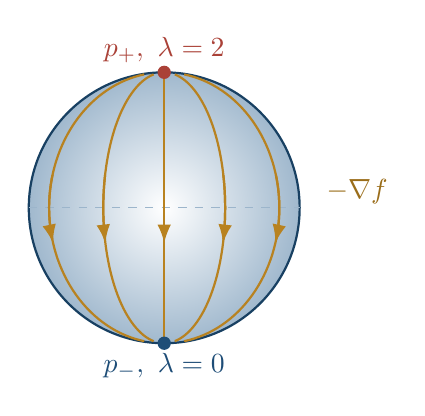
\begin{tikzpicture}[>=Latex,scale=1]
 \shade[inner color=white,outer color=manifoldblue!43]
   (0,0) circle (1.72);
 \draw[manifoldblue!70!black,thick] (0,0) circle (1.72);
 % W tym rzucie prostopadłym równik jest odcinkiem.
 \draw[manifoldblue!45,dashed] (-1.72,0)--(1.72,0);
 % Rzuty południków: (R cos(phi) sin(theta), R cos(theta)).
 \foreach \c in {-.85,-.45,0,.45,.85} {
   \draw[manifoldgold!90!black,thick,domain=10:170,samples=65]
      plot ({1.72*\c*sin(\x)},{1.72*cos(\x)});
   \draw[manifoldgold!90!black,thick,->,domain=76:105,samples=20]
      plot ({1.72*\c*sin(\x)},{1.72*cos(\x)});
 }
 \fill[manifoldred] (0,1.72) circle (2.4pt)
    node[above] {$p_+,\ \lambda=2$};
 \fill[manifoldblue!85!black] (0,-1.72) circle (2.4pt)
    node[below] {$p_-,\ \lambda=0$};
 \node[manifoldgold!75!black] at (2.45,.2)
       {$-\nabla f$};
\end{tikzpicture}
\caption{Spadek funkcji wysokości na sferze.
Dla metryki indukowanej trajektorie są południkami
i biegną od maksimum do minimum; rysunek pokazuje ich rzuty.
Południowy punkt jest stabilny w dwóch
wymiarach, a północny niestabilny w dwóch
wymiarach; pozostałe zbiory stabilne
lub niestabilne tych punktów to same punkty.}
\label{fig:przeplyw-morse-sfera-17}
\end{figure}

\section{Warunek Morse'a--Smale'a i przestrzenie trajektorii}
\label{sec:morse-smale-17}

Dwie rozmaitości $W^u(p)$ i $W^s(q)$
mogą spotkać się stycznie. Wtedy
niewielka zmiana metryki zmienia
obraz trajektorii w trudny do
kontrolowania sposób. Warunek
transwersalności usuwa ten problem.

\begin{definicja}[Para Morse'a--Smale'a]
\index{para morsea--smalea@Para Morse'a--Smale'a}
\label{def:ms-17}
Para $(f,g)$ jest \emph{parą Morse'a--Smale'a},
gdy $f$ jest funkcją Morse'a
i dla każdych punktów krytycznych
$p,q$ rozmaitości $W^u(p)$ i $W^s(q)$
przecinają się transwersalnie.
Jeśli $p\ne q$, oznaczamy przez
\[
 \mathcal M(p,q)
 :=(W^u(p)\cap W^s(q))/\R
\]
zbiór trajektorii z $p$ do $q$
z zapomnianym początkiem czasu;
$\R$ działa przez przesunięcie
parametru $t$.
\end{definicja}

\begin{stwierdzenie}[Wymiar trajektorii]
\label{prop:wymiar-ms-17}
Jeśli para jest Morse'a--Smale'a
i $\mathcal M(p,q)$ jest niepusta,
to $\lambda(p)>\lambda(q)$ oraz
\[
 \dim\mathcal M(p,q)
    =\lambda(p)-\lambda(q)-1.
\]
Przy różnicy indeksów równej $1$
trajektorie są izolowane.
\end{stwierdzenie}
\begin{proof}
Transwersalność i
Twierdzenie~\ref{thm:stable-morse-17}
dają
\[
 \dim(W^u(p)\cap W^s(q))
 =\lambda(p)+(n-\lambda(q))-n
 =\lambda(p)-\lambda(q).
\]
W punkcie niekrytycznym przecięcia
wektor $-\nabla f$ jest niezerowy
i styczny do obu rozmaitości,
bo obie są niezmiennicze
przez przepływ. Dlatego
przecięcie ma wymiar co
najmniej $1$; stąd
$\lambda(p)>\lambda(q)$.
Koniecznie $f(p)>f(q)$. Wybierzmy regularne
$s$ między tymi wartościami i oznaczmy
$\Sigma=W^u(p)\cap W^s(q)\cap f^{-1}(s)$.
Każda trajektoria przecina $\Sigma$ dokładnie raz.
Czas tego przecięcia jest gładki, ponieważ
$Xf\ne0$ na poziomicy (twierdzenie o funkcji uwikłanej).
Przepływ daje zatem globalny dyfeomorfizm
\[
 \Sigma\times\R\longrightarrow W^u(p)\cap W^s(q),
 \qquad (z,t)\longmapsto\Phi_t(z).
\]
Przecięcia rozumiemy w strukturach rozmaitości
immersowanych, czyli jako iloczyny włókniste ich
odwzorowań do $M$. Ich różnowartościowość pozwala
utożsamiać punkty z punktami przecięcia w $M$.
W konsekwencji iloraz jest rozmaitością Hausdorffa
dyfeomorficzną z $\Sigma$, o wymiarze mniejszym o jeden.
Samo lokalne odjęcie wymiaru działania nie
wystarczałoby do uzasadnienia tych własności ilorazu.
\end{proof}

\begin{twierdzenie}[Istnienie metryk Morse'a--Smale'a]
\label{thm:gen-ms-17}
Dla ustalonej funkcji Morse'a
na zwartej $M$ można wybrać
metrykę $g$, euklidesową w małych
mapach Morse'a, tak aby
$(f,g)$ była parą
Morse'a--Smale'a. Takie metryki
są gęste wśród metryk
z ustalonym zachowaniem
blisko punktów krytycznych.
\end{twierdzenie}
\begin{proof}
Pokażemy mechanizm
transwersalności, a następnie
zastosujemy
Twierdzenie~\ref{thm:transwersalnosc-param}.
Ustalmy różne punkty krytyczne
$p,q$ z $f(p)>f(q)$ i regularny
poziom $L=f^{-1}(s)$ między nimi.
Ślady $W^u(p)\cap L$ i $W^s(q)\cap L$
są gładkimi rozmaitościami immersowanymi w $L$.
Wybieramy $s$ poza ustalonymi małymi otoczeniami
punktów krytycznych; poniższe perturbacje
nie będą więc zmieniały metryki w tych otoczeniach.
Wystarczy uzyskać ich
transwersalność na $L$.

Na obszarze, gdzie $\dd f\ne0$,
zmiana metryki może dowolnie
zmienić gradient w pierwszym
rzędzie w kierunkach poprzecznych
do trajektorii. Istotnie, dla
$X=-g^{-1}\dd f$ i symetrycznej
perturbacji $h$ metryki mamy
\[
 \left.\frac{\dd}{\dd\varepsilon}
  (- (g+\varepsilon h)^{-1}\dd f)
 \right|_{\varepsilon=0}
  =-g^{-1}hX.
\]
Gdy $X\ne0$, odwzorowanie
$h\mapsto h(X,\cdot)$ z form
symetrycznych na kowektory
jest surjektywne: w bazie
z pierwszym wektorem
równoległym do $X$ możemy
zadać dowolny pierwszy
wiersz i tę samą pierwszą
kolumnę macierzy $h$.
Wybieramy kulkę na tej
trajektorii \emph{tuż ponad} $L$
i perturbację podpartą tylko
w tej kulce. Poniżej $L$
metryka pozostaje taka sama,
więc $W^s(q)\cap L$ nie zmienia
się. Zmiana wektora prędkości
w kierunku stycznym do $L$
zmienia punkt trafienia w $L$
w tym samym kierunku
w pierwszym rzędzie: wynika
to z całkowego równania
dla zlinearyzowanego przepływu;
przy zmniejszaniu kulki
przeniesienie liniowe na
krótkim odcinku zbliża się
do identyczności.
Wpływ perturbacji na
trajektorię zależy gładko
od jej skończenie wielu
parametrów na mocy
gładkiej zależności
rozwiązań ODE od parametrów.

Doprecyzujmy argument gęstości, ponieważ same zbiory
$W^u,W^s$ zależą od metryki. Ustalmy małą sferę
wyjściową $S_p\subset W^u_{\mathrm{loc}}(p)$
i wejściową $S_q\subset W^s_{\mathrm{loc}}(q)$.
Są one niezależne od zmienianej metryki.
Niech $E_g(x)$ oznacza pierwsze trafienie trajektorii
z $x\in S_p$ w $L$, a $D_g(y)$ pierwsze trafienie
trajektorii biegnącej wstecz z $y\in S_q$ w $L$.
Odwzorowania są określone na otwartych zbiorach tych punktów,
które osiągają $L$ w skończonym czasie.
Zależą gładko od punktu i od skończenie wielu
parametrów metryki. Szukany warunek to
transwersalność $(E_g,D_g)$ do przekątnej w $L\times L$.

Dla każdego $N\in\mathbb N$ żądamy transwersalności
we wszystkich przecięciach, których oba czasy
trafienia są nie większe niż $N$.
Jest to warunek otwarty: ewentualny ciąg przecięć
naruszających go przy $g_j\to g$ ma podciąg
zbieżnych punktów na zwartych $S_p,S_q$
i zbieżnych czasów w $[0,N]$; gładka zależność
przepływu przeczyłaby transwersalności dla $g$.
Jest też gęsty. Przy ustalonej metryce zbiór
takich par startowych jest zwarty, więc wystarcza
skończenie wiele małych obszarów perturbacji
opisanych wyżej. Pochodne parametryczne pierwszej
ewaluacji rozpinają $TL$, podczas gdy druga
ewaluacja nie zmienia się. Parametryczna
transwersalność zastosowana w otoczeniu tego
zwartego zbioru daje dowolnie małe perturbacje
spełniające warunek. Nowe przecięcia o czasach
$\leq N$ nie mogą pojawić się poza tym otoczeniem,
co wynika z tego samego argumentu zwartości.

Przestrzeń gładkich metryk o ustalonych wartościach
w otoczeniach krytycznych jest otwartą częścią
zamkniętej afinicznej podprzestrzeni przestrzeni
Fr\'echeta gładkich tensorów symetrycznych.
Ma własność Baire'a. Przecięcie powyższych
otwartych gęstych warunków po wszystkich $N$
jest więc gęste i obejmuje każde przecięcie
o skończonych czasach trafienia.
Małe perturbacje zachowują dodatnią określoność.
Punktów krytycznych jest
skończenie wiele, więc
przeprowadzamy to dla
wszystkich par. Jeśli
$f(p)\leq f(q)$ i $p\ne q$,
trajektoria spadku nie może
biec z $p$ do $q$;
przy $p=q$ lokalne osie
$\{u=0\}$ i $\{v=0\}$
przecinają się transwersalnie
w $p$.
\end{proof}

\begin{figure}[htbp]
\centering
\begin{tikzpicture}[>=Latex,scale=.95]
 \draw[manifoldblue!30,densely dashed]
   (-2.25,.55) .. controls (-.9,.49) and (.9,.61) .. (2.25,.55);
 \draw[manifoldred!80!black,very thick,->]
   (-1.4,1.50) .. controls (-1.23,.55) and (-.48,.1)
                .. (-.1,-.25);
 \draw[manifoldred!80!black,very thick,->]
   (-.1,-.25) .. controls (.13,-.66) and (.58,-1.14)
             .. (.9,-1.41);
 \fill[manifoldred] (-1.4,1.5) circle (2.3pt)
    node[above] {$p$};
 \fill[manifoldgold!85!black] (-.1,-.25) circle (2.3pt)
    node[left] {$r$};
 \fill[manifoldblue!85!black] (.9,-1.41) circle (2.3pt)
    node[below] {$q$};
 \node[manifoldblue!70!black] at (2.65,.55) {$f=s$};
\end{tikzpicture}
\caption{Schemat trajektorii łamanej $p\to r\to q$.
Pojedyncza trajektoria od $p$ do $q$
może się do niej zbliżać, spędzając
coraz więcej czasu blisko $r$.
Taka granica jest punktem brzegowym
jednowymiarowej przestrzeni trajektorii,
gdy różnica indeksów $p,q$ wynosi $2$.}
\label{fig:lamane-trajektorie-morse-17}
\end{figure}

\section{Kompleks Morse'a: homologia z trajektorii}
\label{sec:kompleks-morse-17}

Teraz ustalmy metrykę Morse'a--Smale'a.
Nie mylmy symboli: w \emph{homologii}
stosujemy operator brzegu $\partial$,
zaś $d$ pozostaje dla form
i operatorów kohomologii
z poprzednich rozdziałów.

\begin{lemat}[Zwartość z dopuszczeniem przełamań]
\label{lem:zwartosc-lamana-17}
Z każdego ciągu trajektorii od $p$ do $q$ można wybrać
podciąg zbiegający do skończonego łańcucha trajektorii
$p=r_0\to r_1\to\cdots\to r_\ell=q$.
Zbieżność oznacza gładką zbieżność na zwartych
przedziałach czasu po osobnym przesunięciu czasu
dla każdego niestałego odcinka.
\end{lemat}
\begin{proof}
Wybierzmy regularne poziomy rozdzielające wszystkie
różne wartości krytyczne między $f(q)$ i $f(p)$.
Każda trajektoria przecina każdy z tych poziomów raz.
Zwartość ich skończonego iloczynu daje podciąg,
na którym wszystkie punkty przecięć zbiegają.
Przepływ z każdego punktu granicznego wyznacza
graniczną trajektorię; gładka zależność od danych
początkowych daje wymaganą zbieżność lokalną.
Na zwartym paśmie bez zer $|\nabla f|\geq m>0$,
więc czas jego przejścia nie przekracza
różnicy poziomów podzielonej przez $m^2$.
Tam odcinki graniczne muszą się łączyć.

Nieograniczone czasy mogą zatem występować tylko
w otoczeniach poziomów krytycznych.
Końce granicznych odcinków są punktami krytycznymi
na mocy Stwierdzenia~\ref{prop:spadek-morse-17}.
Trzeba jeszcze wykluczyć, że odcinek przychodzi do
jednego punktu, a następny wychodzi z innego punktu
\emph{tej samej} wartości krytycznej.
Weźmy rozłączne małe kule wokół tych punktów.
Na zwartym obszarze między kulami $|\nabla f|\geq m>0$,
a przejście między różnymi kulami wymaga długości
co najmniej $d>0$. Spadek funkcji na tym przejściu wynosi
\[
 \int |\nabla f|^2\,\dd t
 =\int |\nabla f|\,\dd s\geq md,
\]
gdzie $s$ jest długością łuku. Nie może on zmieścić się
w pasie o szerokości dążącej do zera.
Tak więc oba odcinki mają wspólny punkt krytyczny.
To samo rozumowanie na małych sferach wyjścia
z $p$ i wejścia do $q$ zachowuje końce całego łańcucha.
Każdy niestały odcinek ściśle obniża $f$,
a więc łańcuch ma skończoną długość.

Zapis przez przecięcia z wybranymi poziomami
wyznacza jednoznacznie trajektorię łamaną.
Nadaje zbiorowi takich łańcuchów topologię Hausdorffa
pochodzącą z metryki skończonego iloczynu poziomic.
Powyższy argument stosuje się też do ciągu łańcuchów:
wybieramy podciąg o ustalonej liście punktów
krytycznych i stosujemy go do każdego odcinka.
Domknięcie przestrzeni trajektorii w tym zbiorze,
oznaczane $\overline{\mathcal M}(p,q)$, jest zatem zwarte.
\end{proof}

\begin{lemat}[Zwarta przestrzeń trajektorii indeksu jeden]
\label{lem:fin-morse-17}
Jeśli $\lambda(p)-\lambda(q)=1$,
to $\mathcal M(p,q)$ jest
skończonym zbiorem.
\end{lemat}
\begin{proof}
Przestrzeń jest zerowymiarowa przez
Stwierdzenie~\ref{prop:wymiar-ms-17}.
Każdy odcinek trajektorii łamanej ściśle obniża indeks.
Przy różnicy indeksów $1$ nie ma miejsca na punkt pośredni.
Lemat~\ref{lem:zwartosc-lamana-17} daje więc zwartość
samej $\mathcal M(p,q)$. Zwarta rozmaitość
zerowymiarowa jest skończonym zbiorem.
\end{proof}

Wybierzmy orientację każdej
rozmaitości $W^u(p)$.
Można to zrobić osobno,
bo jest dyfeomorficzna
z przestrzenią euklidesową;
nie wymaga to orientowalności
całego $M$. Dla trajektorii
$\gamma:p\to q$ o różnicy
indeksów $1$ orientacje
obu rozmaitości niestabilnych
i kierunek przepływu określają
znak $\epsilon(\gamma)\in\{\pm1\}$.
Konkretnie w regularnej
poziomicy $L$ jest to znak
poprzecznego przecięcia
$W^u(p)\cap L$ z
$W^s(q)\cap L$;
normalną orientację drugiego czynnika
przenosimy z $T_qW^u(q)$ wzdłuż $W^s(q)$.
Jest to jednoznaczne, ponieważ $W^s(q)$ jest ściągalna.
Orientację $W^u(p)\cap L$ ustalamy regułą
\[
 \operatorname{or}(TW^u(p))
 =\operatorname{or}(X)\otimes
   \operatorname{or}(T(W^u(p)\cap L)).
\]
Dla różnicy indeksów $1$ znak jest zatem znakiem
izomorfizmu z przestrzeni stycznej tego śladu
do zorientowanej przestrzeni normalnej $W^s(q)$.
Przy większej różnicy indeksów orientujemy jądro
tego odwzorowania, czyli $T\mathcal M(p,q)$,
stawiając je przed przestrzenią normalną.
Zmiana orientacji jednego
$W^u(p)$ zmienia znaki
odpowiedniego generatora,
lecz nie grupy homologii.

\begin{definicja}[Kompleks trajektorii Morse'a]
\index{kompleks trajektorii morsea@Kompleks trajektorii Morse'a}
\label{def:kompleks-morse-17}
Grupa $CM_k(f,g;\Z)$ jest wolną
grupą abelową na punktach
$\operatorname{Crit}_k(f)$.
Dla generatora $p$ kładziemy
\begin{equation}\label{eq:brzeg-morse-17}
 \partial^{\mathrm{Mor}}_k p
 :=\sum_{q\in\operatorname{Crit}_{k-1}(f)}
  \left(\sum_{\gamma\in\mathcal M(p,q)}
                    \epsilon(\gamma)\right)q.
\end{equation}
Suma jest skończona przez
Lemat~\ref{lem:fin-morse-17}.
Nad $\mathbb F_2$ zapominamy znaki:
współczynnikiem przy $q$
jest liczba trajektorii modulo $2$.
\end{definicja}

\begin{twierdzenie}[Dlaczego $\partial^2=0$]
\label{thm:brzeg-morse-17}
Operator~\eqref{eq:brzeg-morse-17}
spełnia
$\partial^{\mathrm{Mor}}_{k-1}
 \partial^{\mathrm{Mor}}_k=0$.
\end{twierdzenie}
\begin{proof}
Ustalmy $p$ o indeksie $k$
i $q$ o indeksie $k-2$.
Ze Stwierdzenia~\ref{prop:wymiar-ms-17}
przestrzeń $\mathcal M(p,q)$
jest jednowymiarowa.
Pokażemy, jakie granice
mogą mieć ciągi jej elementów.
Argument ze zwartością
poziomic z
Lematu~\ref{lem:fin-morse-17}
daje podciąg zbieżny
albo trajektorię $p\to q$,
albo trajektorię łamaną.
Każde przełamanie zużywa
co najmniej jednostkę
różnicy indeksów; przy
różnicy $2$ możliwe
jest dokładnie jedno
$p\to r\to q$ z
$\lambda(r)=k-1$.

Wyjaśnijmy, dlaczego każdy taki łańcuch ma
dokładnie jeden kołnierz, a więc jest rzeczywistym końcem.
Oznaczmy $l=\lambda(r)$, $b=n-l$.
Najpierw załóżmy, że metryka w mapie Morse'a jest euklidesowa.
Przekrój wejściowy ma postać $|v|=\delta$, z parametrami
$(u,\theta)$, gdzie $\theta=v/\delta\in S^{b-1}$.
Przekrój wyjściowy $|u|=\delta$ ma parametry
$(\omega,v)$, gdzie $\omega=u/\delta\in S^{l-1}$.
Transwersalność przy ustalonych trajektoriach $p\to r$
i $r\to q$ pozwala zapisać ślady odpowiednich gałęzi jako
\[
 W^u(p)\cap\Sigma_{\rm in}:\quad\theta=A(u),
 \qquad
 W^s(q)\cap\Sigma_{\rm out}:\quad\omega=B(v).
\]
Istotnie, pierwszy ślad ma wymiar $l$ i jest
poprzeczny do $u=0$, a drugi ma wymiar $b$
i jest poprzeczny do $v=0$.
Przy czasie przejścia $T$ i $\rho=e^{-2T}$
lokalne równania przepływu dają
\[
 u_{\rm in}=\delta\rho\omega,\quad
 v_{\rm in}=\delta\theta,\quad
 u_{\rm out}=\delta\omega,\quad
 v_{\rm out}=\delta\rho\theta.
\]
Warunek dopasowania to dokładnie
\begin{equation}\label{eq:sklejanie-morse-17}
 \theta=A(\delta\rho\omega),\qquad
 \omega=B(\delta\rho\theta).
\end{equation}
Przy $\rho=0$ rozwiązaniem jest $(A(0),B(0))$,
a różniczka równań względem współrzędnych kątowych
$(\theta,\omega)$ jest identycznością.
Twierdzenie o funkcji uwikłanej daje zatem
\emph{jedyne} pobliskie rozwiązanie dla każdego małego
$\rho\geq0$. Dla $\rho>0$ jest to trajektoria niełamana,
a $\rho=0$ oznacza zadany łańcuch.
Dla sfer $S^0$ współrzędne kątowe po prostu nie występują.

Ogólna metryka wymaga dodatkowego argumentu;
nie wolno zakładać gładkiej linearyzacji jej gradientu.
Wyprostujmy lokalne rozmaitości stabilną i niestabilną
z Twierdzenia~\ref{thm:stable-morse-17} do osi $u=0,v=0$.
Równania mają teraz postać
$\dot u=A_uu+R_u(u,v)$, $\dot v=A_sv+R_s(u,v)$,
gdzie $R_u(0,v)=R_s(u,0)=0$ i $DR(0)=0$.
W małym pudełku $|u|,|v|\leq\delta$ norma $u$
ściśle rośnie, a norma $v$ ściśle maleje poza odpowiednią osią.
Dla warunków mieszanych $v(0)=a$, $u(T)=b_0$
wariacja stałych daje
\begin{align*}
 u(t)&=e^{A_u(t-T)}b_0-
       \int_t^T e^{A_u(t-\tau)}R_u(u(\tau),v(\tau))\,\dd\tau,\\
 v(t)&=e^{A_st}a+
       \int_0^t e^{A_s(t-\tau)}R_s(u(\tau),v(\tau))\,\dd\tau.
\end{align*}
Tak jak w dowodzie rozmaitości stabilnej,
małość $DR$ czyni ten operator kontrakcją,
jednostajnie względem $T$.
Stosujemy normę ważoną
\[
 \sup_{0\leq t\leq T}
 \bigl(e^{\eta(T-t)}|u(t)|+e^{\eta t}|v(t)|\bigr),
 \qquad 0<\eta<\alpha.
\]
Znikanie $R_u$ na osi stabilnej i $R_s$ na osi
niestabilnej kontroluje wyrazy mieszane: na kuli
tej normy pochodne mieszane są ograniczone przez
stałą razy $\delta e^{-\eta(T-t)}$ lub
$\delta e^{-\eta t}$. Całkowanie jąder wykładniczych
daje stałą kontrakcji mniejszą od $1$ dla małego $\delta$.
Różniczkowanie równania punktu stałego daje
te same oszacowania dla pochodnych po $a,b_0$.
W szczególności odwzorowania
\[
 U_T(a,b_0)=u(0),\qquad V_T(a,b_0)=v(T)
\]
dążą do zera w normie $C^1$ z szybkością
$O(e^{-\eta T})$ na małych ustalonych zbiorach parametrów.
Zależą gładko od $T<\infty$; można to zobaczyć,
przenosząc równania całkowe na ustalony przedział $[0,1]$.

Równania dopasowania zastępujemy teraz przez
\[
 \theta=A(U_T(\delta\theta,\delta\omega)),\qquad
 \omega=B(V_T(\delta\theta,\delta\omega)).
\]
Dla dużego $T$ ich prawa strona jest kontrakcją
w małym iloczynie map wokół $(A(0),B(0))$.
Istnieje więc dokładnie jedno rozwiązanie,
gładkie dla skończonego $T$ i zbieżne do rozwiązania
łamanego dla $T\to\infty$.
Parametr $1/T\geq0$ daje topologiczny kołnierz końca,
gładki w jego wnętrzu. Możemy go przyjąć za mapę
gładkiej struktury rozmaitości z brzegiem.
Nie potrzebujemy tu gładkości odwzorowania ewaluacji
w zmiennej $1/T$ na samym brzegu.
Jedyność rozwiązania i monotoniczność norm zapewniają,
że wszystkie dostatecznie bliskie trajektorie
są opisane przez ten kołnierz.
Wspomniany argument
zwartości wyklucza inne
końce. Dodając je,
otrzymujemy zwartą
rozmaitość jednowymiarową
z brzegiem
\[
 \partial\overline{\mathcal M}(p,q)
  =\coprod_{\lambda(r)=k-1}
      \mathcal M(p,r)\times\mathcal M(r,q).
\]
Orientacje ustalone przed
Definicją~\ref{def:kompleks-morse-17} orientują wnętrze
tej rozmaitości. Porównanie z orientacją końca można
przeprowadzić na powyższych równaniach dopasowania.
Parametryzacje obu wykresów wnoszą znaki
$\epsilon(\gamma_{pr})$ i $\epsilon(\gamma_{rq})$,
a macierz dopasowania dąży do identyczności,
więc jej wyznacznik jest dodatni.
Pozostaje przestawienie bloków: kierunku przepływu,
parametru kołnierza i przestrzeni normalnych.
Jego znak zależy tylko od wymiarów $k,n$, nie od
trajektorii ani od $r$ (wszystkie te $r$ mają indeks $k-1$).
Dlatego znak punktu brzegowego jest
\[
 \sigma_{k,n}\,
 \epsilon(\gamma_{pr})\epsilon(\gamma_{rq}),
 \qquad \sigma_{k,n}\in\{1,-1\},
\]
z jednym wspólnym czynnikiem konwencji orientacyjnej.
W przypadku ogólnej metryki macierz dopasowania
również dąży do identyczności, więc porównanie jest to samo.
Każdy zwarty zorientowany odcinek ma dwa końce
o przeciwnych znakach, a okrąg nie ma brzegu.
Suma znaków brzegu jest zerem; po pomnożeniu przez
$\sigma_{k,n}$ dostajemy
\[
 \sum_{\lambda(r)=k-1}
 \sum_{\gamma_{pr},\gamma_{rq}}
 \epsilon(\gamma_{pr})\epsilon(\gamma_{rq})=0.
\]
Jest to dokładnie współczynnik przy $q$ w
$\partial^{\mathrm{Mor}}\partial^{\mathrm{Mor}}p$.
Po redukcji modulo $2$
to samo rozumowanie
mówi, że liczba
końców jest parzysta.
\end{proof}

\begin{twierdzenie}[Homologia Morse'a jest homologią $M$]
\label{thm:homologia-morse-17}
Dla zamkniętej rozmaitości
i pary Morse'a--Smale'a
\[
 H_k(CM_\bullet(f,g;\Z),
          \partial^{\mathrm{Mor}})
       \cong H_k(M;\Z).
\]
Wynik nie zależy od
wybranego $f$, metryki
ani orientacji generatorów.
\end{twierdzenie}
\begin{proof}
\emph{Krok 1: filtracja według indeksu.}
Sama zgodność liczby generatorów z liczbą komórek
nie porównuje różniczek. Potrzebna jest ponadto
filtracja uporządkowana według indeksów.
Użyjemy geometrycznego twierdzenia o przestawianiu
wartości krytycznych, którego dowód znajduje się
w Twierdzeniu~\ref{thm:przestawianie-18}.
To odwołanie naprzód nie tworzy koła: tamten argument
używa przepływu i braku trajektorii między zamienianymi
punktami, a nie homologii Morse'a.
W konstrukcji zmieniamy funkcję, zachowując pole $X$:
nierówność $X\widetilde f<0$ pozostaje prawdziwa
poza punktami krytycznymi, a blisko nich dodajemy
do $f$ tylko stałe.

Jeśli dwa sąsiednie punkty w kolejności wartości
mają indeksy malejące, od wyższego punktu
(o mniejszym indeksie) do niższego nie biegnie
trajektoria przez Stwierdzenie~\ref{prop:wymiar-ms-17}.
Można więc zamienić ich wartości. Skończenie wiele
takich zamian daje funkcję $F$, której wszystkie
punkty indeksu $k$ leżą poniżej wszystkich punktów
indeksu $k+1$. Równe wartości można najpierw rozdzielić
małymi zmianami stałymi blisko punktów krytycznych.
Pole $X$ i jego trajektorie oraz ich znaki pozostają te same.
Jeśli chcemy ponownie używać języka gradientu,
poza zerami kładziemy
\[
 \widetilde g(X,X)=-\dd F(X)>0,\qquad
 \widetilde g(X,\ker\dd F)=0,
\]
a na $\ker\dd F$ wybieramy dowolną dodatnią metrykę.
Blisko zer pozostawiamy $g$; sklejenie metryk podziałem
jedności zachowuje liniową tożsamość
$\widetilde g(X,\cdot)=-\dd F$.
Zatem $X=-\nabla_{\widetilde g}F$.

Wybierzmy regularne poziomy $a_k$ po wszystkich
punktach indeksu $k$, a przed punktami wyższych indeksów.
Niech $N_k=F^{-1}(( -\infty,a_k])$,
$N_{-1}=\varnothing$, $N_n=M$.
Twierdzenie o uchwycie i wycięcie dają
\[
 H_j(N_k,N_{k-1};\Z)=
 \begin{cases}\Z^{c_k},&j=k,\\0,&j\ne k.\end{cases}
\]
Przy pustej grupie indeksów wybieramy po prostu
dwa poziomy w tym samym regularnym paśmie.
Filtracja jest równoważna filtracji szkieletami
modelu CW: na każdym etapie przybywają wyłącznie
komórki wymiaru $k$. Jej kompleks względny ma więc
grupy $C_k=H_k(N_k,N_{k-1})$ i brzeg
\[
 C_k\xrightarrow{\delta}H_{k-1}(N_{k-1})
       \longrightarrow H_{k-1}(N_{k-1},N_{k-2})=C_{k-1}.
\]
Jak w dowodzie twierdzenia o homologii komórkowej,
dokładne ciągi par identyfikują jego homologię z $H_*(M)$.

\emph{Krok 2: konkretni reprezentanci generatorów.}
Mały dysk w $W^u(p)$, zorientowany wybraną orientacją,
przedłużamy przepływem aż do poziomu $a_{k-1}$.
Każdy punkt jego sfery wyjściowej dociera tam:
w przeciwnym razie granicą byłby punkt o indeksie
co najmniej $k$, sprzecznie ze ścisłym spadkiem indeksu.
Gładki czas trafienia jest ograniczony na zwartej sferze.
Otrzymujemy zanurzony dysk $D_p\subset N_k$
z brzegiem $S_p\subset\partial N_{k-1}$.
Reprezentuje generator odpowiadający uchwytowi $p$:
lokalnie jego przestrzeń styczna jest ujemną przestrzenią
hesjanu, a więc jego zorientowany dysk jest rdzeniem
generatora lokalnej homologii względnej.
Przedłużenie przez regularny przepływ dodaje tylko kołnierz.

Dla $q$ indeksu $k-1$ analogicznie przedłużamy mały
dysk stabilny wstecz do $\partial N_{k-1}$.
Dostajemy \emph{współrdzeń} $E_q$ uchwytu $q$
i jego brzeg $B_q\subset\partial N_{k-1}$,
nazywany sferą pasa. Nie może on zatrzymać się
przy innym punkcie indeksu $k-1$, bo nie ma
trajektorii między równymi indeksami.
Normalną orientację $E_q$ wyznacza $W^u(q)$.
W małym modelu uchwytu rdzeń i współrdzeń przecinają
się raz, ze znakiem $+1$ przy zgodnych orientacjach.
Jest to lokalna dualność, która pozwala odczytać
współczynnik generatora w $H_{k-1}(N_{k-1},N_{k-2})$.

\emph{Krok 3: porównanie współczynników.}
Obraz $[D_p]$ przez $\delta$ to $[S_p]$.
Jego współczynnik przy $q$ liczymy jako podpisaną
liczbę przecięć $S_p$ z $B_q$ w $\partial N_{k-1}$.
Dlaczego ten rachunek daje współczynnik względny?
W otoczeniu tubularnym współrdzenia rzut na normalny
dysk, po zgnieceniu jego brzegu, mierzy lokalny stopień.
Wycięcie redukuje go do pary uchwytu i jego części
przyczepianej, gdzie rdzeń daje stopień $1$,
a pozostałe generatory dają $0$.
Jest to dokładnie funkcjonał dualny do generatora $q$.
Poprzeczność pozwala obliczać stopień jako sumę
lokalnych znaków, również bez orientowania całego $M$;
wystarczają orientacja $S_p$ i koorientacja $B_q$.

Punkty $S_p\cap B_q$ odpowiadają bijektywnie
trajektoriom $p\to q$, gdyż każda przecina ten
regularny poziom dokładnie raz. Orientacja brzegu
$D_p$ jest określona przez zewnętrzny kierunek $X$,
więc zgadza się z przyjętą orientacją $S_p$.
Koorientacja $B_q$ jest tą samą, której użyliśmy
w definicji $\epsilon(\gamma)$. Współczynnik brzegu
jest zatem dokładnie sumą w~\eqref{eq:brzeg-morse-17}.
Kompleks filtracji jest izomorficzny z kompleksem Morse'a
przez przypisanie $p\mapsto[D_p]$.
Każdy wybór $f,g$ oblicza w ten sposób homologię $M$,
a odwrócenie orientacji $W^u(p)$ zmienia jedynie znak
odpowiedniego generatora.
\end{proof}

\begin{przyklad}[Kompleks na sferze i torusie]
Na $S^2$ z wysokością
z Przykładu~\ref{prz:morse-sfera-17}
nie ma punktów indeksu $1$,
więc
$CM_2=\Z$, $CM_1=0$,
$CM_0=\Z$, a $\partial=0$.
Homologie to $\Z,0,\Z$.

Na torusie z
Przykładu~\ref{prz:morse-torus-17}
mamy
$CM_2=\Z$, $CM_1=\Z^2$,
$CM_0=\Z$. Znamy
$H_0(T^2;\Z)=\Z$,
$H_1(T^2;\Z)=\Z^2$,
$H_2(T^2;\Z)=\Z$;
po przejściu do $\Q$
liczby punktów krytycznych
są już równe liczbom
Betti'ego. Wzór
\eqref{eq:ranki-morse-17}
zmusza wszystkie
$r_k$ do zera.
Macierze całkowite
o zerowym rzędzie
nad $\Q$ są zerowe,
więc $\partial=0$
również nad $\Z$.
Geometrycznie podpisane
liczby trajektorii między
sąsiednimi indeksami
znoszą się w sumie.
\end{przyklad}

\section{Jak to prowadzi do Smale'a i chirurgii?}
\label{sec:morse-most-17}

Funkcja Morse'a opisuje rozmaitość
przez uchwyty. Dla kobordyzmu
$W$ między $M_-$ i $M_+$
analogicznie wybiera się funkcję
stałą na składowych brzegu;
jej punkty krytyczne dają
uchwyty dołączane do
$M_-\times[0,1]$.
Skoro dołączenie uchwytu
indeksu $\lambda$ zmienia
topologię określonego
obszaru, można pytać,
kiedy sąsiednie uchwyty
się znoszą, kiedy da
się przestawiać ich
kolejność i jakie
przeszkody pozostają.
To są kolejne kroki
na drodze do twierdzenia
o $h$-kobordyzmie
Smale'a i teorii chirurgii.

Na rozmaitości niezwartej
właściwa funkcja Morse'a
z Twierdzenia~\ref{thm:wlasciwa-morse-15}
daje analogiczny opis
\emph{po jednym zwartym
paśmie naraz}. Dla
rozmaitości z brzegiem
trzeba kontrolować
kierunek gradientu
przy brzegu i ewentualne
punkty krytyczne
funkcji ograniczonej
do brzegu. Wyniki
tego rozdziału zostały
sformułowane dla
zamkniętej $M$ właśnie
po to, aby takich
warunków nie ukrywać.

\par\smallskip
{\footnotesize\noindent\emph{Dalsza lektura:}
\href{https://math.stanford.edu/~ralph/morsecourse/biglectures.pdf}{R.\ Cohen, \emph{Morse Theory}, lemat Morse'a, uchwyty i nierówności},
\href{https://people.maths.ox.ac.uk/ritter/morse-cambridge/full.pdf}{A.\ Ritter, \emph{Morse Homology}, trajektorie i ich zliczanie},
\href{https://arxiv.org/pdf/math/0411465}{J.\ Weber, \emph{The Morse--Witten complex via dynamical systems}, zwartość, sklejanie i orientacje},
\href{https://ocw.mit.edu/courses/18-965-geometry-of-manifolds-fall-2004/pages/lecture-notes/}{MIT OCW, wykłady z geometrii rozmaitości}.\par}


\clearpage
\phantomsection
\addcontentsline{toc}{chapter}{Indeks pojęć}
\fancyhead[R]{\small Indeks}
\printindex

\end{document}
